% Encyclopaedia of Derivation-like Maps.
% Version: v0.18 (2026-11-08) — every cited work resolves to a file that opens or
% says why it cannot; four defects the citation judge led to were corrected, and the
% path-algebra derivations of Adrabi, Bennis and Fahid were added. v0.17 (2026-11-07) — the parts rebalanced: two parts that held a
% single chapter are folded into their neighbours, and the seven-chapter part
% is split at the natural boundary. No part now holds fewer than two.
\documentclass[11pt,openright,twoside]{memoir}
\usepackage{style/encyclopaedia}

\begin{document}
\frontmatter
% Front cover.
%
% LIGHT ground, so the book looks like a mathematics book and not a thriller.
% Cream paper, deep indigo type, one warm accent that carries the figure.
%
% THE PICTURE. 300 tangents to the astroid, each faint, piling up at the four
% cusps into a star that no line in the family contains. A derivation gives
% local linear data; the curve is what that data builds. Drawn in the accent
% colour so it reads as an engraving on paper rather than as light in the dark.
%
% Literal millimetres, 170 x 240 mm trim.
\begin{titlingpage}
\thispagestyle{empty}
\begin{tikzpicture}[remember picture,overlay]

  % ------------------------------------------------------------- the paper
  \fill[covercream] (current page.south west) rectangle (current page.north east);

  % A deep indigo band across the foot: the one large colour block, so the page
  % has a base and the eye has somewhere to rest.
  \fill[coverindigo] (current page.south west) rectangle ([yshift=34mm]current page.south east);
  % A thin accent rule separating paper from band.
  \fill[coveraccent] ([yshift=34mm]current page.south west) rectangle ([yshift=35.2mm]current page.south east);

  % ------------------------------------------------------------- the figure
  \draw[coveraccent, opacity=0.34, line width=0.30pt] (115.0,75.0) -- (115.0,199.0);
  \draw[coveraccent, opacity=0.34, line width=0.30pt] (118.3,76.8) -- (111.2,200.6);
  \draw[coveraccent, opacity=0.34, line width=0.30pt] (121.1,78.7) -- (107.0,201.9);
  \draw[coveraccent, opacity=0.34, line width=0.30pt] (123.4,80.7) -- (102.3,202.9);
  \draw[coveraccent, opacity=0.34, line width=0.30pt] (125.3,82.7) -- (97.2,203.5);
  \draw[coveraccent, opacity=0.34, line width=0.30pt] (126.7,84.6) -- (91.7,203.6);
  \draw[coveraccent, opacity=0.34, line width=0.30pt] (127.7,86.4) -- (86.0,203.2);
  \draw[coveraccent, opacity=0.34, line width=0.30pt] (128.4,88.0) -- (80.1,202.2);
  \draw[coveraccent, opacity=0.34, line width=0.30pt] (128.8,89.4) -- (74.1,200.7);
  \draw[coveraccent, opacity=0.34, line width=0.30pt] (129.0,90.6) -- (68.0,198.6);
  \draw[coveraccent, opacity=0.34, line width=0.30pt] (129.0,91.6) -- (62.0,195.9);
  \draw[coveraccent, opacity=0.34, line width=0.30pt] (128.9,92.3) -- (56.1,192.6);
  \draw[coveraccent, opacity=0.34, line width=0.30pt] (128.9,92.8) -- (50.4,188.8);
  \draw[coveraccent, opacity=0.34, line width=0.30pt] (128.8,93.1) -- (45.0,184.4);
  \draw[coveraccent, opacity=0.34, line width=0.30pt] (128.9,93.2) -- (39.9,179.6);
  \draw[coveraccent, opacity=0.34, line width=0.30pt] (129.1,93.2) -- (35.3,174.4);
  \draw[coveraccent, opacity=0.34, line width=0.30pt] (129.4,93.1) -- (31.2,168.8);
  \draw[coveraccent, opacity=0.34, line width=0.30pt] (130.0,93.0) -- (27.7,163.0);
  \draw[coveraccent, opacity=0.34, line width=0.30pt] (130.9,93.0) -- (24.7,157.0);
  \draw[coveraccent, opacity=0.34, line width=0.30pt] (131.9,93.1) -- (22.3,151.0);
  \draw[coveraccent, opacity=0.34, line width=0.30pt] (133.2,93.4) -- (20.4,144.9);
  \draw[coveraccent, opacity=0.34, line width=0.30pt] (134.8,93.9) -- (19.2,138.9);
  \draw[coveraccent, opacity=0.34, line width=0.30pt] (136.5,94.8) -- (18.5,133.1);
  \draw[coveraccent, opacity=0.34, line width=0.30pt] (138.3,96.0) -- (18.4,127.5);
  \draw[coveraccent, opacity=0.34, line width=0.30pt] (140.3,97.6) -- (18.7,122.2);
  \draw[coveraccent, opacity=0.34, line width=0.30pt] (142.3,99.7) -- (19.5,117.3);
  \draw[coveraccent, opacity=0.34, line width=0.30pt] (144.2,102.2) -- (20.7,112.9);
  \draw[coveraccent, opacity=0.34, line width=0.30pt] (146.1,105.3) -- (22.2,108.8);
  \draw[coveraccent, opacity=0.34, line width=0.30pt] (147.8,108.8) -- (23.9,105.3);
  \draw[coveraccent, opacity=0.34, line width=0.30pt] (149.3,112.9) -- (25.8,102.2);
  \draw[coveraccent, opacity=0.34, line width=0.30pt] (150.5,117.3) -- (27.7,99.7);
  \draw[coveraccent, opacity=0.34, line width=0.30pt] (151.3,122.2) -- (29.7,97.6);
  \draw[coveraccent, opacity=0.34, line width=0.30pt] (151.6,127.5) -- (31.7,96.0);
  \draw[coveraccent, opacity=0.34, line width=0.30pt] (151.5,133.1) -- (33.5,94.8);
  \draw[coveraccent, opacity=0.34, line width=0.30pt] (150.8,138.9) -- (35.2,93.9);
  \draw[coveraccent, opacity=0.34, line width=0.30pt] (149.6,144.9) -- (36.8,93.4);
  \draw[coveraccent, opacity=0.34, line width=0.30pt] (147.7,151.0) -- (38.1,93.1);
  \draw[coveraccent, opacity=0.34, line width=0.30pt] (145.3,157.0) -- (39.1,93.0);
  \draw[coveraccent, opacity=0.34, line width=0.30pt] (142.3,163.0) -- (40.0,93.0);
  \draw[coveraccent, opacity=0.34, line width=0.30pt] (138.8,168.8) -- (40.6,93.1);
  \draw[coveraccent, opacity=0.34, line width=0.30pt] (134.7,174.4) -- (40.9,93.2);
  \draw[coveraccent, opacity=0.34, line width=0.30pt] (130.1,179.6) -- (41.1,93.2);
  \draw[coveraccent, opacity=0.34, line width=0.30pt] (125.0,184.4) -- (41.2,93.1);
  \draw[coveraccent, opacity=0.34, line width=0.30pt] (119.6,188.8) -- (41.1,92.8);
  \draw[coveraccent, opacity=0.34, line width=0.30pt] (113.9,192.6) -- (41.1,92.3);
  \draw[coveraccent, opacity=0.34, line width=0.30pt] (108.0,195.9) -- (41.0,91.6);
  \draw[coveraccent, opacity=0.34, line width=0.30pt] (102.0,198.6) -- (41.0,90.6);
  \draw[coveraccent, opacity=0.34, line width=0.30pt] (95.9,200.7) -- (41.2,89.4);
  \draw[coveraccent, opacity=0.34, line width=0.30pt] (89.9,202.2) -- (41.6,88.0);
  \draw[coveraccent, opacity=0.34, line width=0.30pt] (84.0,203.2) -- (42.3,86.4);
  \draw[coveraccent, opacity=0.34, line width=0.30pt] (78.3,203.6) -- (43.3,84.6);
  \draw[coveraccent, opacity=0.34, line width=0.30pt] (72.8,203.5) -- (44.7,82.7);
  \draw[coveraccent, opacity=0.34, line width=0.30pt] (67.7,202.9) -- (46.6,80.7);
  \draw[coveraccent, opacity=0.34, line width=0.30pt] (63.0,201.9) -- (48.9,78.7);
  \draw[coveraccent, opacity=0.34, line width=0.30pt] (58.8,200.6) -- (51.7,76.8);
  \draw[coveraccent, opacity=0.34, line width=0.30pt] (55.0,199.0) -- (55.0,75.0);
  \draw[coveraccent, opacity=0.34, line width=0.30pt] (51.7,197.2) -- (58.8,73.4);
  \draw[coveraccent, opacity=0.34, line width=0.30pt] (48.9,195.3) -- (63.0,72.1);
  \draw[coveraccent, opacity=0.34, line width=0.30pt] (46.6,193.3) -- (67.7,71.1);
  \draw[coveraccent, opacity=0.34, line width=0.30pt] (44.7,191.3) -- (72.8,70.5);
  \draw[coveraccent, opacity=0.34, line width=0.30pt] (43.3,189.4) -- (78.3,70.4);
  \draw[coveraccent, opacity=0.34, line width=0.30pt] (42.3,187.6) -- (84.0,70.8);
  \draw[coveraccent, opacity=0.34, line width=0.30pt] (41.6,186.0) -- (89.9,71.8);
  \draw[coveraccent, opacity=0.34, line width=0.30pt] (41.2,184.6) -- (95.9,73.3);
  \draw[coveraccent, opacity=0.34, line width=0.30pt] (41.0,183.4) -- (102.0,75.4);
  \draw[coveraccent, opacity=0.34, line width=0.30pt] (41.0,182.4) -- (108.0,78.1);
  \draw[coveraccent, opacity=0.34, line width=0.30pt] (41.1,181.7) -- (113.9,81.4);
  \draw[coveraccent, opacity=0.34, line width=0.30pt] (41.1,181.2) -- (119.6,85.2);
  \draw[coveraccent, opacity=0.34, line width=0.30pt] (41.2,180.9) -- (125.0,89.6);
  \draw[coveraccent, opacity=0.34, line width=0.30pt] (41.1,180.8) -- (130.1,94.4);
  \draw[coveraccent, opacity=0.34, line width=0.30pt] (40.9,180.8) -- (134.7,99.6);
  \draw[coveraccent, opacity=0.34, line width=0.30pt] (40.6,180.9) -- (138.8,105.2);
  \draw[coveraccent, opacity=0.34, line width=0.30pt] (40.0,181.0) -- (142.3,111.0);
  \draw[coveraccent, opacity=0.34, line width=0.30pt] (39.1,181.0) -- (145.3,117.0);
  \draw[coveraccent, opacity=0.34, line width=0.30pt] (38.1,180.9) -- (147.7,123.0);
  \draw[coveraccent, opacity=0.34, line width=0.30pt] (36.8,180.6) -- (149.6,129.1);
  \draw[coveraccent, opacity=0.34, line width=0.30pt] (35.2,180.1) -- (150.8,135.1);
  \draw[coveraccent, opacity=0.34, line width=0.30pt] (33.5,179.2) -- (151.5,140.9);
  \draw[coveraccent, opacity=0.34, line width=0.30pt] (31.7,178.0) -- (151.6,146.5);
  \draw[coveraccent, opacity=0.34, line width=0.30pt] (29.7,176.4) -- (151.3,151.8);
  \draw[coveraccent, opacity=0.34, line width=0.30pt] (27.7,174.3) -- (150.5,156.7);
  \draw[coveraccent, opacity=0.34, line width=0.30pt] (25.8,171.8) -- (149.3,161.1);
  \draw[coveraccent, opacity=0.34, line width=0.30pt] (23.9,168.7) -- (147.8,165.2);
  \draw[coveraccent, opacity=0.34, line width=0.30pt] (22.2,165.2) -- (146.1,168.7);
  \draw[coveraccent, opacity=0.34, line width=0.30pt] (20.7,161.1) -- (144.2,171.8);
  \draw[coveraccent, opacity=0.34, line width=0.30pt] (19.5,156.7) -- (142.3,174.3);
  \draw[coveraccent, opacity=0.34, line width=0.30pt] (18.7,151.8) -- (140.3,176.4);
  \draw[coveraccent, opacity=0.34, line width=0.30pt] (18.4,146.5) -- (138.3,178.0);
  \draw[coveraccent, opacity=0.34, line width=0.30pt] (18.5,140.9) -- (136.5,179.2);
  \draw[coveraccent, opacity=0.34, line width=0.30pt] (19.2,135.1) -- (134.8,180.1);
  \draw[coveraccent, opacity=0.34, line width=0.30pt] (20.4,129.1) -- (133.2,180.6);
  \draw[coveraccent, opacity=0.34, line width=0.30pt] (22.3,123.0) -- (131.9,180.9);
  \draw[coveraccent, opacity=0.34, line width=0.30pt] (24.7,117.0) -- (130.9,181.0);
  \draw[coveraccent, opacity=0.34, line width=0.30pt] (27.7,111.0) -- (130.0,181.0);
  \draw[coveraccent, opacity=0.34, line width=0.30pt] (31.2,105.2) -- (129.4,180.9);
  \draw[coveraccent, opacity=0.34, line width=0.30pt] (35.3,99.6) -- (129.1,180.8);
  \draw[coveraccent, opacity=0.34, line width=0.30pt] (39.9,94.4) -- (128.9,180.8);
  \draw[coveraccent, opacity=0.34, line width=0.30pt] (45.0,89.6) -- (128.8,180.9);
  \draw[coveraccent, opacity=0.34, line width=0.30pt] (50.4,85.2) -- (128.9,181.2);
  \draw[coveraccent, opacity=0.34, line width=0.30pt] (56.1,81.4) -- (128.9,181.7);
  \draw[coveraccent, opacity=0.34, line width=0.30pt] (62.0,78.1) -- (129.0,182.4);
  \draw[coveraccent, opacity=0.34, line width=0.30pt] (68.0,75.4) -- (129.0,183.4);
  \draw[coveraccent, opacity=0.34, line width=0.30pt] (74.1,73.3) -- (128.8,184.6);
  \draw[coveraccent, opacity=0.34, line width=0.30pt] (80.1,71.8) -- (128.4,186.0);
  \draw[coveraccent, opacity=0.34, line width=0.30pt] (86.0,70.8) -- (127.7,187.6);
  \draw[coveraccent, opacity=0.34, line width=0.30pt] (91.7,70.4) -- (126.7,189.4);
  \draw[coveraccent, opacity=0.34, line width=0.30pt] (97.2,70.5) -- (125.3,191.3);
  \draw[coveraccent, opacity=0.34, line width=0.30pt] (102.3,71.1) -- (123.4,193.3);
  \draw[coveraccent, opacity=0.34, line width=0.30pt] (107.0,72.1) -- (121.1,195.3);
  \draw[coveraccent, opacity=0.34, line width=0.30pt] (111.2,73.4) -- (118.3,197.2);

  \draw[coveraccent, opacity=0.22, line width=7pt, line cap=round] (115.0,137.0) -- (115.0,137.0) -- (115.0,137.0) -- (115.0,137.0) -- (114.9,137.0) -- (114.9,137.0) -- (114.9,137.0) -- (114.8,137.0) -- (114.8,137.0) -- (114.7,137.0) -- (114.7,137.0) -- (114.6,137.0) -- (114.5,137.0) -- (114.4,137.0) -- (114.3,137.1) -- (114.2,137.1) -- (114.1,137.1) -- (114.0,137.1) -- (113.9,137.1) -- (113.8,137.1) -- (113.7,137.2) -- (113.5,137.2) -- (113.4,137.2) -- (113.2,137.2) -- (113.1,137.3) -- (112.9,137.3) -- (112.8,137.3) -- (112.6,137.4) -- (112.4,137.4) -- (112.2,137.5) -- (112.0,137.5) -- (111.8,137.6) -- (111.6,137.6) -- (111.4,137.7) -- (111.2,137.7) -- (111.0,137.8) -- (110.8,137.9) -- (110.6,138.0) -- (110.4,138.0) -- (110.1,138.1) -- (109.9,138.2) -- (109.7,138.3) -- (109.4,138.4) -- (109.2,138.5) -- (108.9,138.6) -- (108.7,138.7) -- (108.4,138.8) -- (108.1,138.9) -- (107.9,139.0) -- (107.6,139.1) -- (107.3,139.3) -- (107.1,139.4) -- (106.8,139.5) -- (106.5,139.7) -- (106.2,139.8) -- (105.9,140.0) -- (105.7,140.1) -- (105.4,140.3) -- (105.1,140.4) -- (104.8,140.6) -- (104.5,140.8) -- (104.2,140.9) -- (103.9,141.1) -- (103.6,141.3) -- (103.3,141.5) -- (103.0,141.7) -- (102.7,141.8) -- (102.4,142.0) -- (102.1,142.2) -- (101.8,142.5) -- (101.5,142.7) -- (101.2,142.9) -- (100.9,143.1) -- (100.6,143.3) -- (100.3,143.5) -- (100.0,143.8) -- (99.7,144.0) -- (99.4,144.2) -- (99.1,144.5) -- (98.8,144.7) -- (98.5,145.0) -- (98.2,145.2) -- (97.9,145.5) -- (97.6,145.7) -- (97.3,146.0) -- (97.0,146.3) -- (96.7,146.5) -- (96.5,146.8) -- (96.2,147.1) -- (95.9,147.3) -- (95.6,147.6) -- (95.3,147.9) -- (95.1,148.2) -- (94.8,148.5) -- (94.5,148.7) -- (94.3,149.0) -- (94.0,149.3) -- (93.7,149.6) -- (93.5,149.9) -- (93.2,150.2) -- (93.0,150.5) -- (92.7,150.8) -- (92.5,151.1) -- (92.2,151.4) -- (92.0,151.7) -- (91.8,152.0) -- (91.5,152.3) -- (91.3,152.6) -- (91.1,152.9) -- (90.9,153.2) -- (90.7,153.5) -- (90.5,153.8) -- (90.2,154.1) -- (90.0,154.4) -- (89.8,154.7) -- (89.7,155.0) -- (89.5,155.3) -- (89.3,155.6) -- (89.1,155.9) -- (88.9,156.2) -- (88.8,156.5) -- (88.6,156.8) -- (88.4,157.1) -- (88.3,157.4) -- (88.1,157.7) -- (88.0,157.9) -- (87.8,158.2) -- (87.7,158.5) -- (87.5,158.8) -- (87.4,159.1) -- (87.3,159.3) -- (87.1,159.6) -- (87.0,159.9) -- (86.9,160.1) -- (86.8,160.4) -- (86.7,160.7) -- (86.6,160.9) -- (86.5,161.2) -- (86.4,161.4) -- (86.3,161.7) -- (86.2,161.9) -- (86.1,162.1) -- (86.0,162.4) -- (86.0,162.6) -- (85.9,162.8) -- (85.8,163.0) -- (85.7,163.2) -- (85.7,163.4) -- (85.6,163.6) -- (85.6,163.8) -- (85.5,164.0) -- (85.5,164.2) -- (85.4,164.4) -- (85.4,164.6) -- (85.3,164.8) -- (85.3,164.9) -- (85.3,165.1) -- (85.2,165.2) -- (85.2,165.4) -- (85.2,165.5) -- (85.2,165.7) -- (85.1,165.8) -- (85.1,165.9) -- (85.1,166.0) -- (85.1,166.1) -- (85.1,166.2) -- (85.1,166.3) -- (85.0,166.4) -- (85.0,166.5) -- (85.0,166.6) -- (85.0,166.7) -- (85.0,166.7) -- (85.0,166.8) -- (85.0,166.8) -- (85.0,166.9) -- (85.0,166.9) -- (85.0,166.9) -- (85.0,167.0) -- (85.0,167.0) -- (85.0,167.0) -- (85.0,167.0) -- (85.0,167.0) -- (85.0,167.0) -- (85.0,167.0) -- (85.0,166.9) -- (85.0,166.9) -- (85.0,166.9) -- (85.0,166.8) -- (85.0,166.8) -- (85.0,166.7) -- (85.0,166.7) -- (85.0,166.6) -- (85.0,166.5) -- (85.0,166.4) -- (84.9,166.3) -- (84.9,166.2) -- (84.9,166.1) -- (84.9,166.0) -- (84.9,165.9) -- (84.9,165.8) -- (84.8,165.7) -- (84.8,165.5) -- (84.8,165.4) -- (84.8,165.2) -- (84.7,165.1) -- (84.7,164.9) -- (84.7,164.8) -- (84.6,164.6) -- (84.6,164.4) -- (84.5,164.2) -- (84.5,164.0) -- (84.4,163.8) -- (84.4,163.6) -- (84.3,163.4) -- (84.3,163.2) -- (84.2,163.0) -- (84.1,162.8) -- (84.0,162.6) -- (84.0,162.4) -- (83.9,162.1) -- (83.8,161.9) -- (83.7,161.7) -- (83.6,161.4) -- (83.5,161.2) -- (83.4,160.9) -- (83.3,160.7) -- (83.2,160.4) -- (83.1,160.1) -- (83.0,159.9) -- (82.9,159.6) -- (82.7,159.3) -- (82.6,159.1) -- (82.5,158.8) -- (82.3,158.5) -- (82.2,158.2) -- (82.0,157.9) -- (81.9,157.7) -- (81.7,157.4) -- (81.6,157.1) -- (81.4,156.8) -- (81.2,156.5) -- (81.1,156.2) -- (80.9,155.9) -- (80.7,155.6) -- (80.5,155.3) -- (80.3,155.0) -- (80.2,154.7) -- (80.0,154.4) -- (79.8,154.1) -- (79.5,153.8) -- (79.3,153.5) -- (79.1,153.2) -- (78.9,152.9) -- (78.7,152.6) -- (78.5,152.3) -- (78.2,152.0) -- (78.0,151.7) -- (77.8,151.4) -- (77.5,151.1) -- (77.3,150.8) -- (77.0,150.5) -- (76.8,150.2) -- (76.5,149.9) -- (76.3,149.6) -- (76.0,149.3) -- (75.7,149.0) -- (75.5,148.7) -- (75.2,148.5) -- (74.9,148.2) -- (74.7,147.9) -- (74.4,147.6) -- (74.1,147.3) -- (73.8,147.1) -- (73.5,146.8) -- (73.3,146.5) -- (73.0,146.3) -- (72.7,146.0) -- (72.4,145.7) -- (72.1,145.5) -- (71.8,145.2) -- (71.5,145.0) -- (71.2,144.7) -- (70.9,144.5) -- (70.6,144.2) -- (70.3,144.0) -- (70.0,143.8) -- (69.7,143.5) -- (69.4,143.3) -- (69.1,143.1) -- (68.8,142.9) -- (68.5,142.7) -- (68.2,142.5) -- (67.9,142.2) -- (67.6,142.0) -- (67.3,141.8) -- (67.0,141.7) -- (66.7,141.5) -- (66.4,141.3) -- (66.1,141.1) -- (65.8,140.9) -- (65.5,140.8) -- (65.2,140.6) -- (64.9,140.4) -- (64.6,140.3) -- (64.3,140.1) -- (64.1,140.0) -- (63.8,139.8) -- (63.5,139.7) -- (63.2,139.5) -- (62.9,139.4) -- (62.7,139.3) -- (62.4,139.1) -- (62.1,139.0) -- (61.9,138.9) -- (61.6,138.8) -- (61.3,138.7) -- (61.1,138.6) -- (60.8,138.5) -- (60.6,138.4) -- (60.3,138.3) -- (60.1,138.2) -- (59.9,138.1) -- (59.6,138.0) -- (59.4,138.0) -- (59.2,137.9) -- (59.0,137.8) -- (58.8,137.7) -- (58.6,137.7) -- (58.4,137.6) -- (58.2,137.6) -- (58.0,137.5) -- (57.8,137.5) -- (57.6,137.4) -- (57.4,137.4) -- (57.2,137.3) -- (57.1,137.3) -- (56.9,137.3) -- (56.8,137.2) -- (56.6,137.2) -- (56.5,137.2) -- (56.3,137.2) -- (56.2,137.1) -- (56.1,137.1) -- (56.0,137.1) -- (55.9,137.1) -- (55.8,137.1) -- (55.7,137.1) -- (55.6,137.0) -- (55.5,137.0) -- (55.4,137.0) -- (55.3,137.0) -- (55.3,137.0) -- (55.2,137.0) -- (55.2,137.0) -- (55.1,137.0) -- (55.1,137.0) -- (55.1,137.0) -- (55.0,137.0) -- (55.0,137.0) -- (55.0,137.0) -- (55.0,137.0) -- (55.0,137.0) -- (55.0,137.0) -- (55.0,137.0) -- (55.1,137.0) -- (55.1,137.0) -- (55.1,137.0) -- (55.2,137.0) -- (55.2,137.0) -- (55.3,137.0) -- (55.3,137.0) -- (55.4,137.0) -- (55.5,137.0) -- (55.6,137.0) -- (55.7,136.9) -- (55.8,136.9) -- (55.9,136.9) -- (56.0,136.9) -- (56.1,136.9) -- (56.2,136.9) -- (56.3,136.8) -- (56.5,136.8) -- (56.6,136.8) -- (56.8,136.8) -- (56.9,136.7) -- (57.1,136.7) -- (57.2,136.7) -- (57.4,136.6) -- (57.6,136.6) -- (57.8,136.5) -- (58.0,136.5) -- (58.2,136.4) -- (58.4,136.4) -- (58.6,136.3) -- (58.8,136.3) -- (59.0,136.2) -- (59.2,136.1) -- (59.4,136.0) -- (59.6,136.0) -- (59.9,135.9) -- (60.1,135.8) -- (60.3,135.7) -- (60.6,135.6) -- (60.8,135.5) -- (61.1,135.4) -- (61.3,135.3) -- (61.6,135.2) -- (61.9,135.1) -- (62.1,135.0) -- (62.4,134.9) -- (62.7,134.7) -- (62.9,134.6) -- (63.2,134.5) -- (63.5,134.3) -- (63.8,134.2) -- (64.1,134.0) -- (64.3,133.9) -- (64.6,133.7) -- (64.9,133.6) -- (65.2,133.4) -- (65.5,133.2) -- (65.8,133.1) -- (66.1,132.9) -- (66.4,132.7) -- (66.7,132.5) -- (67.0,132.3) -- (67.3,132.2) -- (67.6,132.0) -- (67.9,131.8) -- (68.2,131.5) -- (68.5,131.3) -- (68.8,131.1) -- (69.1,130.9) -- (69.4,130.7) -- (69.7,130.5) -- (70.0,130.2) -- (70.3,130.0) -- (70.6,129.8) -- (70.9,129.5) -- (71.2,129.3) -- (71.5,129.0) -- (71.8,128.8) -- (72.1,128.5) -- (72.4,128.3) -- (72.7,128.0) -- (73.0,127.7) -- (73.3,127.5) -- (73.5,127.2) -- (73.8,126.9) -- (74.1,126.7) -- (74.4,126.4) -- (74.7,126.1) -- (74.9,125.8) -- (75.2,125.5) -- (75.5,125.3) -- (75.7,125.0) -- (76.0,124.7) -- (76.3,124.4) -- (76.5,124.1) -- (76.8,123.8) -- (77.0,123.5) -- (77.3,123.2) -- (77.5,122.9) -- (77.8,122.6) -- (78.0,122.3) -- (78.2,122.0) -- (78.5,121.7) -- (78.7,121.4) -- (78.9,121.1) -- (79.1,120.8) -- (79.3,120.5) -- (79.5,120.2) -- (79.8,119.9) -- (80.0,119.6) -- (80.2,119.3) -- (80.3,119.0) -- (80.5,118.7) -- (80.7,118.4) -- (80.9,118.1) -- (81.1,117.8) -- (81.2,117.5) -- (81.4,117.2) -- (81.6,116.9) -- (81.7,116.6) -- (81.9,116.3) -- (82.0,116.1) -- (82.2,115.8) -- (82.3,115.5) -- (82.5,115.2) -- (82.6,114.9) -- (82.7,114.7) -- (82.9,114.4) -- (83.0,114.1) -- (83.1,113.9) -- (83.2,113.6) -- (83.3,113.3) -- (83.4,113.1) -- (83.5,112.8) -- (83.6,112.6) -- (83.7,112.3) -- (83.8,112.1) -- (83.9,111.9) -- (84.0,111.6) -- (84.0,111.4) -- (84.1,111.2) -- (84.2,111.0) -- (84.3,110.8) -- (84.3,110.6) -- (84.4,110.4) -- (84.4,110.2) -- (84.5,110.0) -- (84.5,109.8) -- (84.6,109.6) -- (84.6,109.4) -- (84.7,109.2) -- (84.7,109.1) -- (84.7,108.9) -- (84.8,108.8) -- (84.8,108.6) -- (84.8,108.5) -- (84.8,108.3) -- (84.9,108.2) -- (84.9,108.1) -- (84.9,108.0) -- (84.9,107.9) -- (84.9,107.8) -- (84.9,107.7) -- (85.0,107.6) -- (85.0,107.5) -- (85.0,107.4) -- (85.0,107.3) -- (85.0,107.3) -- (85.0,107.2) -- (85.0,107.2) -- (85.0,107.1) -- (85.0,107.1) -- (85.0,107.1) -- (85.0,107.0) -- (85.0,107.0) -- (85.0,107.0) -- (85.0,107.0) -- (85.0,107.0) -- (85.0,107.0) -- (85.0,107.0) -- (85.0,107.1) -- (85.0,107.1) -- (85.0,107.1) -- (85.0,107.2) -- (85.0,107.2) -- (85.0,107.3) -- (85.0,107.3) -- (85.0,107.4) -- (85.0,107.5) -- (85.0,107.6) -- (85.1,107.7) -- (85.1,107.8) -- (85.1,107.9) -- (85.1,108.0) -- (85.1,108.1) -- (85.1,108.2) -- (85.2,108.3) -- (85.2,108.5) -- (85.2,108.6) -- (85.2,108.8) -- (85.3,108.9) -- (85.3,109.1) -- (85.3,109.2) -- (85.4,109.4) -- (85.4,109.6) -- (85.5,109.8) -- (85.5,110.0) -- (85.6,110.2) -- (85.6,110.4) -- (85.7,110.6) -- (85.7,110.8) -- (85.8,111.0) -- (85.9,111.2) -- (86.0,111.4) -- (86.0,111.6) -- (86.1,111.9) -- (86.2,112.1) -- (86.3,112.3) -- (86.4,112.6) -- (86.5,112.8) -- (86.6,113.1) -- (86.7,113.3) -- (86.8,113.6) -- (86.9,113.9) -- (87.0,114.1) -- (87.1,114.4) -- (87.3,114.7) -- (87.4,114.9) -- (87.5,115.2) -- (87.7,115.5) -- (87.8,115.8) -- (88.0,116.1) -- (88.1,116.3) -- (88.3,116.6) -- (88.4,116.9) -- (88.6,117.2) -- (88.8,117.5) -- (88.9,117.8) -- (89.1,118.1) -- (89.3,118.4) -- (89.5,118.7) -- (89.7,119.0) -- (89.8,119.3) -- (90.0,119.6) -- (90.2,119.9) -- (90.5,120.2) -- (90.7,120.5) -- (90.9,120.8) -- (91.1,121.1) -- (91.3,121.4) -- (91.5,121.7) -- (91.8,122.0) -- (92.0,122.3) -- (92.2,122.6) -- (92.5,122.9) -- (92.7,123.2) -- (93.0,123.5) -- (93.2,123.8) -- (93.5,124.1) -- (93.7,124.4) -- (94.0,124.7) -- (94.3,125.0) -- (94.5,125.3) -- (94.8,125.5) -- (95.1,125.8) -- (95.3,126.1) -- (95.6,126.4) -- (95.9,126.7) -- (96.2,126.9) -- (96.5,127.2) -- (96.7,127.5) -- (97.0,127.7) -- (97.3,128.0) -- (97.6,128.3) -- (97.9,128.5) -- (98.2,128.8) -- (98.5,129.0) -- (98.8,129.3) -- (99.1,129.5) -- (99.4,129.8) -- (99.7,130.0) -- (100.0,130.2) -- (100.3,130.5) -- (100.6,130.7) -- (100.9,130.9) -- (101.2,131.1) -- (101.5,131.3) -- (101.8,131.5) -- (102.1,131.8) -- (102.4,132.0) -- (102.7,132.2) -- (103.0,132.3) -- (103.3,132.5) -- (103.6,132.7) -- (103.9,132.9) -- (104.2,133.1) -- (104.5,133.2) -- (104.8,133.4) -- (105.1,133.6) -- (105.4,133.7) -- (105.7,133.9) -- (105.9,134.0) -- (106.2,134.2) -- (106.5,134.3) -- (106.8,134.5) -- (107.1,134.6) -- (107.3,134.7) -- (107.6,134.9) -- (107.9,135.0) -- (108.1,135.1) -- (108.4,135.2) -- (108.7,135.3) -- (108.9,135.4) -- (109.2,135.5) -- (109.4,135.6) -- (109.7,135.7) -- (109.9,135.8) -- (110.1,135.9) -- (110.4,136.0) -- (110.6,136.0) -- (110.8,136.1) -- (111.0,136.2) -- (111.2,136.3) -- (111.4,136.3) -- (111.6,136.4) -- (111.8,136.4) -- (112.0,136.5) -- (112.2,136.5) -- (112.4,136.6) -- (112.6,136.6) -- (112.8,136.7) -- (112.9,136.7) -- (113.1,136.7) -- (113.2,136.8) -- (113.4,136.8) -- (113.5,136.8) -- (113.7,136.8) -- (113.8,136.9) -- (113.9,136.9) -- (114.0,136.9) -- (114.1,136.9) -- (114.2,136.9) -- (114.3,136.9) -- (114.4,137.0) -- (114.5,137.0) -- (114.6,137.0) -- (114.7,137.0) -- (114.7,137.0) -- (114.8,137.0) -- (114.8,137.0) -- (114.9,137.0) -- (114.9,137.0) -- (114.9,137.0) -- (115.0,137.0) -- (115.0,137.0) -- (115.0,137.0) -- (115.0,137.0);
  \draw[coveraccent, opacity=0.65, line width=2.8pt, line cap=round] (115.0,137.0) -- (115.0,137.0) -- (115.0,137.0) -- (115.0,137.0) -- (114.9,137.0) -- (114.9,137.0) -- (114.9,137.0) -- (114.8,137.0) -- (114.8,137.0) -- (114.7,137.0) -- (114.7,137.0) -- (114.6,137.0) -- (114.5,137.0) -- (114.4,137.0) -- (114.3,137.1) -- (114.2,137.1) -- (114.1,137.1) -- (114.0,137.1) -- (113.9,137.1) -- (113.8,137.1) -- (113.7,137.2) -- (113.5,137.2) -- (113.4,137.2) -- (113.2,137.2) -- (113.1,137.3) -- (112.9,137.3) -- (112.8,137.3) -- (112.6,137.4) -- (112.4,137.4) -- (112.2,137.5) -- (112.0,137.5) -- (111.8,137.6) -- (111.6,137.6) -- (111.4,137.7) -- (111.2,137.7) -- (111.0,137.8) -- (110.8,137.9) -- (110.6,138.0) -- (110.4,138.0) -- (110.1,138.1) -- (109.9,138.2) -- (109.7,138.3) -- (109.4,138.4) -- (109.2,138.5) -- (108.9,138.6) -- (108.7,138.7) -- (108.4,138.8) -- (108.1,138.9) -- (107.9,139.0) -- (107.6,139.1) -- (107.3,139.3) -- (107.1,139.4) -- (106.8,139.5) -- (106.5,139.7) -- (106.2,139.8) -- (105.9,140.0) -- (105.7,140.1) -- (105.4,140.3) -- (105.1,140.4) -- (104.8,140.6) -- (104.5,140.8) -- (104.2,140.9) -- (103.9,141.1) -- (103.6,141.3) -- (103.3,141.5) -- (103.0,141.7) -- (102.7,141.8) -- (102.4,142.0) -- (102.1,142.2) -- (101.8,142.5) -- (101.5,142.7) -- (101.2,142.9) -- (100.9,143.1) -- (100.6,143.3) -- (100.3,143.5) -- (100.0,143.8) -- (99.7,144.0) -- (99.4,144.2) -- (99.1,144.5) -- (98.8,144.7) -- (98.5,145.0) -- (98.2,145.2) -- (97.9,145.5) -- (97.6,145.7) -- (97.3,146.0) -- (97.0,146.3) -- (96.7,146.5) -- (96.5,146.8) -- (96.2,147.1) -- (95.9,147.3) -- (95.6,147.6) -- (95.3,147.9) -- (95.1,148.2) -- (94.8,148.5) -- (94.5,148.7) -- (94.3,149.0) -- (94.0,149.3) -- (93.7,149.6) -- (93.5,149.9) -- (93.2,150.2) -- (93.0,150.5) -- (92.7,150.8) -- (92.5,151.1) -- (92.2,151.4) -- (92.0,151.7) -- (91.8,152.0) -- (91.5,152.3) -- (91.3,152.6) -- (91.1,152.9) -- (90.9,153.2) -- (90.7,153.5) -- (90.5,153.8) -- (90.2,154.1) -- (90.0,154.4) -- (89.8,154.7) -- (89.7,155.0) -- (89.5,155.3) -- (89.3,155.6) -- (89.1,155.9) -- (88.9,156.2) -- (88.8,156.5) -- (88.6,156.8) -- (88.4,157.1) -- (88.3,157.4) -- (88.1,157.7) -- (88.0,157.9) -- (87.8,158.2) -- (87.7,158.5) -- (87.5,158.8) -- (87.4,159.1) -- (87.3,159.3) -- (87.1,159.6) -- (87.0,159.9) -- (86.9,160.1) -- (86.8,160.4) -- (86.7,160.7) -- (86.6,160.9) -- (86.5,161.2) -- (86.4,161.4) -- (86.3,161.7) -- (86.2,161.9) -- (86.1,162.1) -- (86.0,162.4) -- (86.0,162.6) -- (85.9,162.8) -- (85.8,163.0) -- (85.7,163.2) -- (85.7,163.4) -- (85.6,163.6) -- (85.6,163.8) -- (85.5,164.0) -- (85.5,164.2) -- (85.4,164.4) -- (85.4,164.6) -- (85.3,164.8) -- (85.3,164.9) -- (85.3,165.1) -- (85.2,165.2) -- (85.2,165.4) -- (85.2,165.5) -- (85.2,165.7) -- (85.1,165.8) -- (85.1,165.9) -- (85.1,166.0) -- (85.1,166.1) -- (85.1,166.2) -- (85.1,166.3) -- (85.0,166.4) -- (85.0,166.5) -- (85.0,166.6) -- (85.0,166.7) -- (85.0,166.7) -- (85.0,166.8) -- (85.0,166.8) -- (85.0,166.9) -- (85.0,166.9) -- (85.0,166.9) -- (85.0,167.0) -- (85.0,167.0) -- (85.0,167.0) -- (85.0,167.0) -- (85.0,167.0) -- (85.0,167.0) -- (85.0,167.0) -- (85.0,166.9) -- (85.0,166.9) -- (85.0,166.9) -- (85.0,166.8) -- (85.0,166.8) -- (85.0,166.7) -- (85.0,166.7) -- (85.0,166.6) -- (85.0,166.5) -- (85.0,166.4) -- (84.9,166.3) -- (84.9,166.2) -- (84.9,166.1) -- (84.9,166.0) -- (84.9,165.9) -- (84.9,165.8) -- (84.8,165.7) -- (84.8,165.5) -- (84.8,165.4) -- (84.8,165.2) -- (84.7,165.1) -- (84.7,164.9) -- (84.7,164.8) -- (84.6,164.6) -- (84.6,164.4) -- (84.5,164.2) -- (84.5,164.0) -- (84.4,163.8) -- (84.4,163.6) -- (84.3,163.4) -- (84.3,163.2) -- (84.2,163.0) -- (84.1,162.8) -- (84.0,162.6) -- (84.0,162.4) -- (83.9,162.1) -- (83.8,161.9) -- (83.7,161.7) -- (83.6,161.4) -- (83.5,161.2) -- (83.4,160.9) -- (83.3,160.7) -- (83.2,160.4) -- (83.1,160.1) -- (83.0,159.9) -- (82.9,159.6) -- (82.7,159.3) -- (82.6,159.1) -- (82.5,158.8) -- (82.3,158.5) -- (82.2,158.2) -- (82.0,157.9) -- (81.9,157.7) -- (81.7,157.4) -- (81.6,157.1) -- (81.4,156.8) -- (81.2,156.5) -- (81.1,156.2) -- (80.9,155.9) -- (80.7,155.6) -- (80.5,155.3) -- (80.3,155.0) -- (80.2,154.7) -- (80.0,154.4) -- (79.8,154.1) -- (79.5,153.8) -- (79.3,153.5) -- (79.1,153.2) -- (78.9,152.9) -- (78.7,152.6) -- (78.5,152.3) -- (78.2,152.0) -- (78.0,151.7) -- (77.8,151.4) -- (77.5,151.1) -- (77.3,150.8) -- (77.0,150.5) -- (76.8,150.2) -- (76.5,149.9) -- (76.3,149.6) -- (76.0,149.3) -- (75.7,149.0) -- (75.5,148.7) -- (75.2,148.5) -- (74.9,148.2) -- (74.7,147.9) -- (74.4,147.6) -- (74.1,147.3) -- (73.8,147.1) -- (73.5,146.8) -- (73.3,146.5) -- (73.0,146.3) -- (72.7,146.0) -- (72.4,145.7) -- (72.1,145.5) -- (71.8,145.2) -- (71.5,145.0) -- (71.2,144.7) -- (70.9,144.5) -- (70.6,144.2) -- (70.3,144.0) -- (70.0,143.8) -- (69.7,143.5) -- (69.4,143.3) -- (69.1,143.1) -- (68.8,142.9) -- (68.5,142.7) -- (68.2,142.5) -- (67.9,142.2) -- (67.6,142.0) -- (67.3,141.8) -- (67.0,141.7) -- (66.7,141.5) -- (66.4,141.3) -- (66.1,141.1) -- (65.8,140.9) -- (65.5,140.8) -- (65.2,140.6) -- (64.9,140.4) -- (64.6,140.3) -- (64.3,140.1) -- (64.1,140.0) -- (63.8,139.8) -- (63.5,139.7) -- (63.2,139.5) -- (62.9,139.4) -- (62.7,139.3) -- (62.4,139.1) -- (62.1,139.0) -- (61.9,138.9) -- (61.6,138.8) -- (61.3,138.7) -- (61.1,138.6) -- (60.8,138.5) -- (60.6,138.4) -- (60.3,138.3) -- (60.1,138.2) -- (59.9,138.1) -- (59.6,138.0) -- (59.4,138.0) -- (59.2,137.9) -- (59.0,137.8) -- (58.8,137.7) -- (58.6,137.7) -- (58.4,137.6) -- (58.2,137.6) -- (58.0,137.5) -- (57.8,137.5) -- (57.6,137.4) -- (57.4,137.4) -- (57.2,137.3) -- (57.1,137.3) -- (56.9,137.3) -- (56.8,137.2) -- (56.6,137.2) -- (56.5,137.2) -- (56.3,137.2) -- (56.2,137.1) -- (56.1,137.1) -- (56.0,137.1) -- (55.9,137.1) -- (55.8,137.1) -- (55.7,137.1) -- (55.6,137.0) -- (55.5,137.0) -- (55.4,137.0) -- (55.3,137.0) -- (55.3,137.0) -- (55.2,137.0) -- (55.2,137.0) -- (55.1,137.0) -- (55.1,137.0) -- (55.1,137.0) -- (55.0,137.0) -- (55.0,137.0) -- (55.0,137.0) -- (55.0,137.0) -- (55.0,137.0) -- (55.0,137.0) -- (55.0,137.0) -- (55.1,137.0) -- (55.1,137.0) -- (55.1,137.0) -- (55.2,137.0) -- (55.2,137.0) -- (55.3,137.0) -- (55.3,137.0) -- (55.4,137.0) -- (55.5,137.0) -- (55.6,137.0) -- (55.7,136.9) -- (55.8,136.9) -- (55.9,136.9) -- (56.0,136.9) -- (56.1,136.9) -- (56.2,136.9) -- (56.3,136.8) -- (56.5,136.8) -- (56.6,136.8) -- (56.8,136.8) -- (56.9,136.7) -- (57.1,136.7) -- (57.2,136.7) -- (57.4,136.6) -- (57.6,136.6) -- (57.8,136.5) -- (58.0,136.5) -- (58.2,136.4) -- (58.4,136.4) -- (58.6,136.3) -- (58.8,136.3) -- (59.0,136.2) -- (59.2,136.1) -- (59.4,136.0) -- (59.6,136.0) -- (59.9,135.9) -- (60.1,135.8) -- (60.3,135.7) -- (60.6,135.6) -- (60.8,135.5) -- (61.1,135.4) -- (61.3,135.3) -- (61.6,135.2) -- (61.9,135.1) -- (62.1,135.0) -- (62.4,134.9) -- (62.7,134.7) -- (62.9,134.6) -- (63.2,134.5) -- (63.5,134.3) -- (63.8,134.2) -- (64.1,134.0) -- (64.3,133.9) -- (64.6,133.7) -- (64.9,133.6) -- (65.2,133.4) -- (65.5,133.2) -- (65.8,133.1) -- (66.1,132.9) -- (66.4,132.7) -- (66.7,132.5) -- (67.0,132.3) -- (67.3,132.2) -- (67.6,132.0) -- (67.9,131.8) -- (68.2,131.5) -- (68.5,131.3) -- (68.8,131.1) -- (69.1,130.9) -- (69.4,130.7) -- (69.7,130.5) -- (70.0,130.2) -- (70.3,130.0) -- (70.6,129.8) -- (70.9,129.5) -- (71.2,129.3) -- (71.5,129.0) -- (71.8,128.8) -- (72.1,128.5) -- (72.4,128.3) -- (72.7,128.0) -- (73.0,127.7) -- (73.3,127.5) -- (73.5,127.2) -- (73.8,126.9) -- (74.1,126.7) -- (74.4,126.4) -- (74.7,126.1) -- (74.9,125.8) -- (75.2,125.5) -- (75.5,125.3) -- (75.7,125.0) -- (76.0,124.7) -- (76.3,124.4) -- (76.5,124.1) -- (76.8,123.8) -- (77.0,123.5) -- (77.3,123.2) -- (77.5,122.9) -- (77.8,122.6) -- (78.0,122.3) -- (78.2,122.0) -- (78.5,121.7) -- (78.7,121.4) -- (78.9,121.1) -- (79.1,120.8) -- (79.3,120.5) -- (79.5,120.2) -- (79.8,119.9) -- (80.0,119.6) -- (80.2,119.3) -- (80.3,119.0) -- (80.5,118.7) -- (80.7,118.4) -- (80.9,118.1) -- (81.1,117.8) -- (81.2,117.5) -- (81.4,117.2) -- (81.6,116.9) -- (81.7,116.6) -- (81.9,116.3) -- (82.0,116.1) -- (82.2,115.8) -- (82.3,115.5) -- (82.5,115.2) -- (82.6,114.9) -- (82.7,114.7) -- (82.9,114.4) -- (83.0,114.1) -- (83.1,113.9) -- (83.2,113.6) -- (83.3,113.3) -- (83.4,113.1) -- (83.5,112.8) -- (83.6,112.6) -- (83.7,112.3) -- (83.8,112.1) -- (83.9,111.9) -- (84.0,111.6) -- (84.0,111.4) -- (84.1,111.2) -- (84.2,111.0) -- (84.3,110.8) -- (84.3,110.6) -- (84.4,110.4) -- (84.4,110.2) -- (84.5,110.0) -- (84.5,109.8) -- (84.6,109.6) -- (84.6,109.4) -- (84.7,109.2) -- (84.7,109.1) -- (84.7,108.9) -- (84.8,108.8) -- (84.8,108.6) -- (84.8,108.5) -- (84.8,108.3) -- (84.9,108.2) -- (84.9,108.1) -- (84.9,108.0) -- (84.9,107.9) -- (84.9,107.8) -- (84.9,107.7) -- (85.0,107.6) -- (85.0,107.5) -- (85.0,107.4) -- (85.0,107.3) -- (85.0,107.3) -- (85.0,107.2) -- (85.0,107.2) -- (85.0,107.1) -- (85.0,107.1) -- (85.0,107.1) -- (85.0,107.0) -- (85.0,107.0) -- (85.0,107.0) -- (85.0,107.0) -- (85.0,107.0) -- (85.0,107.0) -- (85.0,107.0) -- (85.0,107.1) -- (85.0,107.1) -- (85.0,107.1) -- (85.0,107.2) -- (85.0,107.2) -- (85.0,107.3) -- (85.0,107.3) -- (85.0,107.4) -- (85.0,107.5) -- (85.0,107.6) -- (85.1,107.7) -- (85.1,107.8) -- (85.1,107.9) -- (85.1,108.0) -- (85.1,108.1) -- (85.1,108.2) -- (85.2,108.3) -- (85.2,108.5) -- (85.2,108.6) -- (85.2,108.8) -- (85.3,108.9) -- (85.3,109.1) -- (85.3,109.2) -- (85.4,109.4) -- (85.4,109.6) -- (85.5,109.8) -- (85.5,110.0) -- (85.6,110.2) -- (85.6,110.4) -- (85.7,110.6) -- (85.7,110.8) -- (85.8,111.0) -- (85.9,111.2) -- (86.0,111.4) -- (86.0,111.6) -- (86.1,111.9) -- (86.2,112.1) -- (86.3,112.3) -- (86.4,112.6) -- (86.5,112.8) -- (86.6,113.1) -- (86.7,113.3) -- (86.8,113.6) -- (86.9,113.9) -- (87.0,114.1) -- (87.1,114.4) -- (87.3,114.7) -- (87.4,114.9) -- (87.5,115.2) -- (87.7,115.5) -- (87.8,115.8) -- (88.0,116.1) -- (88.1,116.3) -- (88.3,116.6) -- (88.4,116.9) -- (88.6,117.2) -- (88.8,117.5) -- (88.9,117.8) -- (89.1,118.1) -- (89.3,118.4) -- (89.5,118.7) -- (89.7,119.0) -- (89.8,119.3) -- (90.0,119.6) -- (90.2,119.9) -- (90.5,120.2) -- (90.7,120.5) -- (90.9,120.8) -- (91.1,121.1) -- (91.3,121.4) -- (91.5,121.7) -- (91.8,122.0) -- (92.0,122.3) -- (92.2,122.6) -- (92.5,122.9) -- (92.7,123.2) -- (93.0,123.5) -- (93.2,123.8) -- (93.5,124.1) -- (93.7,124.4) -- (94.0,124.7) -- (94.3,125.0) -- (94.5,125.3) -- (94.8,125.5) -- (95.1,125.8) -- (95.3,126.1) -- (95.6,126.4) -- (95.9,126.7) -- (96.2,126.9) -- (96.5,127.2) -- (96.7,127.5) -- (97.0,127.7) -- (97.3,128.0) -- (97.6,128.3) -- (97.9,128.5) -- (98.2,128.8) -- (98.5,129.0) -- (98.8,129.3) -- (99.1,129.5) -- (99.4,129.8) -- (99.7,130.0) -- (100.0,130.2) -- (100.3,130.5) -- (100.6,130.7) -- (100.9,130.9) -- (101.2,131.1) -- (101.5,131.3) -- (101.8,131.5) -- (102.1,131.8) -- (102.4,132.0) -- (102.7,132.2) -- (103.0,132.3) -- (103.3,132.5) -- (103.6,132.7) -- (103.9,132.9) -- (104.2,133.1) -- (104.5,133.2) -- (104.8,133.4) -- (105.1,133.6) -- (105.4,133.7) -- (105.7,133.9) -- (105.9,134.0) -- (106.2,134.2) -- (106.5,134.3) -- (106.8,134.5) -- (107.1,134.6) -- (107.3,134.7) -- (107.6,134.9) -- (107.9,135.0) -- (108.1,135.1) -- (108.4,135.2) -- (108.7,135.3) -- (108.9,135.4) -- (109.2,135.5) -- (109.4,135.6) -- (109.7,135.7) -- (109.9,135.8) -- (110.1,135.9) -- (110.4,136.0) -- (110.6,136.0) -- (110.8,136.1) -- (111.0,136.2) -- (111.2,136.3) -- (111.4,136.3) -- (111.6,136.4) -- (111.8,136.4) -- (112.0,136.5) -- (112.2,136.5) -- (112.4,136.6) -- (112.6,136.6) -- (112.8,136.7) -- (112.9,136.7) -- (113.1,136.7) -- (113.2,136.8) -- (113.4,136.8) -- (113.5,136.8) -- (113.7,136.8) -- (113.8,136.9) -- (113.9,136.9) -- (114.0,136.9) -- (114.1,136.9) -- (114.2,136.9) -- (114.3,136.9) -- (114.4,137.0) -- (114.5,137.0) -- (114.6,137.0) -- (114.7,137.0) -- (114.7,137.0) -- (114.8,137.0) -- (114.8,137.0) -- (114.9,137.0) -- (114.9,137.0) -- (114.9,137.0) -- (115.0,137.0) -- (115.0,137.0) -- (115.0,137.0) -- (115.0,137.0);
  \draw[coveraccent!55!black, line width=0.9pt, line cap=round] (115.0,137.0) -- (115.0,137.0) -- (115.0,137.0) -- (115.0,137.0) -- (114.9,137.0) -- (114.9,137.0) -- (114.9,137.0) -- (114.8,137.0) -- (114.8,137.0) -- (114.7,137.0) -- (114.7,137.0) -- (114.6,137.0) -- (114.5,137.0) -- (114.4,137.0) -- (114.3,137.1) -- (114.2,137.1) -- (114.1,137.1) -- (114.0,137.1) -- (113.9,137.1) -- (113.8,137.1) -- (113.7,137.2) -- (113.5,137.2) -- (113.4,137.2) -- (113.2,137.2) -- (113.1,137.3) -- (112.9,137.3) -- (112.8,137.3) -- (112.6,137.4) -- (112.4,137.4) -- (112.2,137.5) -- (112.0,137.5) -- (111.8,137.6) -- (111.6,137.6) -- (111.4,137.7) -- (111.2,137.7) -- (111.0,137.8) -- (110.8,137.9) -- (110.6,138.0) -- (110.4,138.0) -- (110.1,138.1) -- (109.9,138.2) -- (109.7,138.3) -- (109.4,138.4) -- (109.2,138.5) -- (108.9,138.6) -- (108.7,138.7) -- (108.4,138.8) -- (108.1,138.9) -- (107.9,139.0) -- (107.6,139.1) -- (107.3,139.3) -- (107.1,139.4) -- (106.8,139.5) -- (106.5,139.7) -- (106.2,139.8) -- (105.9,140.0) -- (105.7,140.1) -- (105.4,140.3) -- (105.1,140.4) -- (104.8,140.6) -- (104.5,140.8) -- (104.2,140.9) -- (103.9,141.1) -- (103.6,141.3) -- (103.3,141.5) -- (103.0,141.7) -- (102.7,141.8) -- (102.4,142.0) -- (102.1,142.2) -- (101.8,142.5) -- (101.5,142.7) -- (101.2,142.9) -- (100.9,143.1) -- (100.6,143.3) -- (100.3,143.5) -- (100.0,143.8) -- (99.7,144.0) -- (99.4,144.2) -- (99.1,144.5) -- (98.8,144.7) -- (98.5,145.0) -- (98.2,145.2) -- (97.9,145.5) -- (97.6,145.7) -- (97.3,146.0) -- (97.0,146.3) -- (96.7,146.5) -- (96.5,146.8) -- (96.2,147.1) -- (95.9,147.3) -- (95.6,147.6) -- (95.3,147.9) -- (95.1,148.2) -- (94.8,148.5) -- (94.5,148.7) -- (94.3,149.0) -- (94.0,149.3) -- (93.7,149.6) -- (93.5,149.9) -- (93.2,150.2) -- (93.0,150.5) -- (92.7,150.8) -- (92.5,151.1) -- (92.2,151.4) -- (92.0,151.7) -- (91.8,152.0) -- (91.5,152.3) -- (91.3,152.6) -- (91.1,152.9) -- (90.9,153.2) -- (90.7,153.5) -- (90.5,153.8) -- (90.2,154.1) -- (90.0,154.4) -- (89.8,154.7) -- (89.7,155.0) -- (89.5,155.3) -- (89.3,155.6) -- (89.1,155.9) -- (88.9,156.2) -- (88.8,156.5) -- (88.6,156.8) -- (88.4,157.1) -- (88.3,157.4) -- (88.1,157.7) -- (88.0,157.9) -- (87.8,158.2) -- (87.7,158.5) -- (87.5,158.8) -- (87.4,159.1) -- (87.3,159.3) -- (87.1,159.6) -- (87.0,159.9) -- (86.9,160.1) -- (86.8,160.4) -- (86.7,160.7) -- (86.6,160.9) -- (86.5,161.2) -- (86.4,161.4) -- (86.3,161.7) -- (86.2,161.9) -- (86.1,162.1) -- (86.0,162.4) -- (86.0,162.6) -- (85.9,162.8) -- (85.8,163.0) -- (85.7,163.2) -- (85.7,163.4) -- (85.6,163.6) -- (85.6,163.8) -- (85.5,164.0) -- (85.5,164.2) -- (85.4,164.4) -- (85.4,164.6) -- (85.3,164.8) -- (85.3,164.9) -- (85.3,165.1) -- (85.2,165.2) -- (85.2,165.4) -- (85.2,165.5) -- (85.2,165.7) -- (85.1,165.8) -- (85.1,165.9) -- (85.1,166.0) -- (85.1,166.1) -- (85.1,166.2) -- (85.1,166.3) -- (85.0,166.4) -- (85.0,166.5) -- (85.0,166.6) -- (85.0,166.7) -- (85.0,166.7) -- (85.0,166.8) -- (85.0,166.8) -- (85.0,166.9) -- (85.0,166.9) -- (85.0,166.9) -- (85.0,167.0) -- (85.0,167.0) -- (85.0,167.0) -- (85.0,167.0) -- (85.0,167.0) -- (85.0,167.0) -- (85.0,167.0) -- (85.0,166.9) -- (85.0,166.9) -- (85.0,166.9) -- (85.0,166.8) -- (85.0,166.8) -- (85.0,166.7) -- (85.0,166.7) -- (85.0,166.6) -- (85.0,166.5) -- (85.0,166.4) -- (84.9,166.3) -- (84.9,166.2) -- (84.9,166.1) -- (84.9,166.0) -- (84.9,165.9) -- (84.9,165.8) -- (84.8,165.7) -- (84.8,165.5) -- (84.8,165.4) -- (84.8,165.2) -- (84.7,165.1) -- (84.7,164.9) -- (84.7,164.8) -- (84.6,164.6) -- (84.6,164.4) -- (84.5,164.2) -- (84.5,164.0) -- (84.4,163.8) -- (84.4,163.6) -- (84.3,163.4) -- (84.3,163.2) -- (84.2,163.0) -- (84.1,162.8) -- (84.0,162.6) -- (84.0,162.4) -- (83.9,162.1) -- (83.8,161.9) -- (83.7,161.7) -- (83.6,161.4) -- (83.5,161.2) -- (83.4,160.9) -- (83.3,160.7) -- (83.2,160.4) -- (83.1,160.1) -- (83.0,159.9) -- (82.9,159.6) -- (82.7,159.3) -- (82.6,159.1) -- (82.5,158.8) -- (82.3,158.5) -- (82.2,158.2) -- (82.0,157.9) -- (81.9,157.7) -- (81.7,157.4) -- (81.6,157.1) -- (81.4,156.8) -- (81.2,156.5) -- (81.1,156.2) -- (80.9,155.9) -- (80.7,155.6) -- (80.5,155.3) -- (80.3,155.0) -- (80.2,154.7) -- (80.0,154.4) -- (79.8,154.1) -- (79.5,153.8) -- (79.3,153.5) -- (79.1,153.2) -- (78.9,152.9) -- (78.7,152.6) -- (78.5,152.3) -- (78.2,152.0) -- (78.0,151.7) -- (77.8,151.4) -- (77.5,151.1) -- (77.3,150.8) -- (77.0,150.5) -- (76.8,150.2) -- (76.5,149.9) -- (76.3,149.6) -- (76.0,149.3) -- (75.7,149.0) -- (75.5,148.7) -- (75.2,148.5) -- (74.9,148.2) -- (74.7,147.9) -- (74.4,147.6) -- (74.1,147.3) -- (73.8,147.1) -- (73.5,146.8) -- (73.3,146.5) -- (73.0,146.3) -- (72.7,146.0) -- (72.4,145.7) -- (72.1,145.5) -- (71.8,145.2) -- (71.5,145.0) -- (71.2,144.7) -- (70.9,144.5) -- (70.6,144.2) -- (70.3,144.0) -- (70.0,143.8) -- (69.7,143.5) -- (69.4,143.3) -- (69.1,143.1) -- (68.8,142.9) -- (68.5,142.7) -- (68.2,142.5) -- (67.9,142.2) -- (67.6,142.0) -- (67.3,141.8) -- (67.0,141.7) -- (66.7,141.5) -- (66.4,141.3) -- (66.1,141.1) -- (65.8,140.9) -- (65.5,140.8) -- (65.2,140.6) -- (64.9,140.4) -- (64.6,140.3) -- (64.3,140.1) -- (64.1,140.0) -- (63.8,139.8) -- (63.5,139.7) -- (63.2,139.5) -- (62.9,139.4) -- (62.7,139.3) -- (62.4,139.1) -- (62.1,139.0) -- (61.9,138.9) -- (61.6,138.8) -- (61.3,138.7) -- (61.1,138.6) -- (60.8,138.5) -- (60.6,138.4) -- (60.3,138.3) -- (60.1,138.2) -- (59.9,138.1) -- (59.6,138.0) -- (59.4,138.0) -- (59.2,137.9) -- (59.0,137.8) -- (58.8,137.7) -- (58.6,137.7) -- (58.4,137.6) -- (58.2,137.6) -- (58.0,137.5) -- (57.8,137.5) -- (57.6,137.4) -- (57.4,137.4) -- (57.2,137.3) -- (57.1,137.3) -- (56.9,137.3) -- (56.8,137.2) -- (56.6,137.2) -- (56.5,137.2) -- (56.3,137.2) -- (56.2,137.1) -- (56.1,137.1) -- (56.0,137.1) -- (55.9,137.1) -- (55.8,137.1) -- (55.7,137.1) -- (55.6,137.0) -- (55.5,137.0) -- (55.4,137.0) -- (55.3,137.0) -- (55.3,137.0) -- (55.2,137.0) -- (55.2,137.0) -- (55.1,137.0) -- (55.1,137.0) -- (55.1,137.0) -- (55.0,137.0) -- (55.0,137.0) -- (55.0,137.0) -- (55.0,137.0) -- (55.0,137.0) -- (55.0,137.0) -- (55.0,137.0) -- (55.1,137.0) -- (55.1,137.0) -- (55.1,137.0) -- (55.2,137.0) -- (55.2,137.0) -- (55.3,137.0) -- (55.3,137.0) -- (55.4,137.0) -- (55.5,137.0) -- (55.6,137.0) -- (55.7,136.9) -- (55.8,136.9) -- (55.9,136.9) -- (56.0,136.9) -- (56.1,136.9) -- (56.2,136.9) -- (56.3,136.8) -- (56.5,136.8) -- (56.6,136.8) -- (56.8,136.8) -- (56.9,136.7) -- (57.1,136.7) -- (57.2,136.7) -- (57.4,136.6) -- (57.6,136.6) -- (57.8,136.5) -- (58.0,136.5) -- (58.2,136.4) -- (58.4,136.4) -- (58.6,136.3) -- (58.8,136.3) -- (59.0,136.2) -- (59.2,136.1) -- (59.4,136.0) -- (59.6,136.0) -- (59.9,135.9) -- (60.1,135.8) -- (60.3,135.7) -- (60.6,135.6) -- (60.8,135.5) -- (61.1,135.4) -- (61.3,135.3) -- (61.6,135.2) -- (61.9,135.1) -- (62.1,135.0) -- (62.4,134.9) -- (62.7,134.7) -- (62.9,134.6) -- (63.2,134.5) -- (63.5,134.3) -- (63.8,134.2) -- (64.1,134.0) -- (64.3,133.9) -- (64.6,133.7) -- (64.9,133.6) -- (65.2,133.4) -- (65.5,133.2) -- (65.8,133.1) -- (66.1,132.9) -- (66.4,132.7) -- (66.7,132.5) -- (67.0,132.3) -- (67.3,132.2) -- (67.6,132.0) -- (67.9,131.8) -- (68.2,131.5) -- (68.5,131.3) -- (68.8,131.1) -- (69.1,130.9) -- (69.4,130.7) -- (69.7,130.5) -- (70.0,130.2) -- (70.3,130.0) -- (70.6,129.8) -- (70.9,129.5) -- (71.2,129.3) -- (71.5,129.0) -- (71.8,128.8) -- (72.1,128.5) -- (72.4,128.3) -- (72.7,128.0) -- (73.0,127.7) -- (73.3,127.5) -- (73.5,127.2) -- (73.8,126.9) -- (74.1,126.7) -- (74.4,126.4) -- (74.7,126.1) -- (74.9,125.8) -- (75.2,125.5) -- (75.5,125.3) -- (75.7,125.0) -- (76.0,124.7) -- (76.3,124.4) -- (76.5,124.1) -- (76.8,123.8) -- (77.0,123.5) -- (77.3,123.2) -- (77.5,122.9) -- (77.8,122.6) -- (78.0,122.3) -- (78.2,122.0) -- (78.5,121.7) -- (78.7,121.4) -- (78.9,121.1) -- (79.1,120.8) -- (79.3,120.5) -- (79.5,120.2) -- (79.8,119.9) -- (80.0,119.6) -- (80.2,119.3) -- (80.3,119.0) -- (80.5,118.7) -- (80.7,118.4) -- (80.9,118.1) -- (81.1,117.8) -- (81.2,117.5) -- (81.4,117.2) -- (81.6,116.9) -- (81.7,116.6) -- (81.9,116.3) -- (82.0,116.1) -- (82.2,115.8) -- (82.3,115.5) -- (82.5,115.2) -- (82.6,114.9) -- (82.7,114.7) -- (82.9,114.4) -- (83.0,114.1) -- (83.1,113.9) -- (83.2,113.6) -- (83.3,113.3) -- (83.4,113.1) -- (83.5,112.8) -- (83.6,112.6) -- (83.7,112.3) -- (83.8,112.1) -- (83.9,111.9) -- (84.0,111.6) -- (84.0,111.4) -- (84.1,111.2) -- (84.2,111.0) -- (84.3,110.8) -- (84.3,110.6) -- (84.4,110.4) -- (84.4,110.2) -- (84.5,110.0) -- (84.5,109.8) -- (84.6,109.6) -- (84.6,109.4) -- (84.7,109.2) -- (84.7,109.1) -- (84.7,108.9) -- (84.8,108.8) -- (84.8,108.6) -- (84.8,108.5) -- (84.8,108.3) -- (84.9,108.2) -- (84.9,108.1) -- (84.9,108.0) -- (84.9,107.9) -- (84.9,107.8) -- (84.9,107.7) -- (85.0,107.6) -- (85.0,107.5) -- (85.0,107.4) -- (85.0,107.3) -- (85.0,107.3) -- (85.0,107.2) -- (85.0,107.2) -- (85.0,107.1) -- (85.0,107.1) -- (85.0,107.1) -- (85.0,107.0) -- (85.0,107.0) -- (85.0,107.0) -- (85.0,107.0) -- (85.0,107.0) -- (85.0,107.0) -- (85.0,107.0) -- (85.0,107.1) -- (85.0,107.1) -- (85.0,107.1) -- (85.0,107.2) -- (85.0,107.2) -- (85.0,107.3) -- (85.0,107.3) -- (85.0,107.4) -- (85.0,107.5) -- (85.0,107.6) -- (85.1,107.7) -- (85.1,107.8) -- (85.1,107.9) -- (85.1,108.0) -- (85.1,108.1) -- (85.1,108.2) -- (85.2,108.3) -- (85.2,108.5) -- (85.2,108.6) -- (85.2,108.8) -- (85.3,108.9) -- (85.3,109.1) -- (85.3,109.2) -- (85.4,109.4) -- (85.4,109.6) -- (85.5,109.8) -- (85.5,110.0) -- (85.6,110.2) -- (85.6,110.4) -- (85.7,110.6) -- (85.7,110.8) -- (85.8,111.0) -- (85.9,111.2) -- (86.0,111.4) -- (86.0,111.6) -- (86.1,111.9) -- (86.2,112.1) -- (86.3,112.3) -- (86.4,112.6) -- (86.5,112.8) -- (86.6,113.1) -- (86.7,113.3) -- (86.8,113.6) -- (86.9,113.9) -- (87.0,114.1) -- (87.1,114.4) -- (87.3,114.7) -- (87.4,114.9) -- (87.5,115.2) -- (87.7,115.5) -- (87.8,115.8) -- (88.0,116.1) -- (88.1,116.3) -- (88.3,116.6) -- (88.4,116.9) -- (88.6,117.2) -- (88.8,117.5) -- (88.9,117.8) -- (89.1,118.1) -- (89.3,118.4) -- (89.5,118.7) -- (89.7,119.0) -- (89.8,119.3) -- (90.0,119.6) -- (90.2,119.9) -- (90.5,120.2) -- (90.7,120.5) -- (90.9,120.8) -- (91.1,121.1) -- (91.3,121.4) -- (91.5,121.7) -- (91.8,122.0) -- (92.0,122.3) -- (92.2,122.6) -- (92.5,122.9) -- (92.7,123.2) -- (93.0,123.5) -- (93.2,123.8) -- (93.5,124.1) -- (93.7,124.4) -- (94.0,124.7) -- (94.3,125.0) -- (94.5,125.3) -- (94.8,125.5) -- (95.1,125.8) -- (95.3,126.1) -- (95.6,126.4) -- (95.9,126.7) -- (96.2,126.9) -- (96.5,127.2) -- (96.7,127.5) -- (97.0,127.7) -- (97.3,128.0) -- (97.6,128.3) -- (97.9,128.5) -- (98.2,128.8) -- (98.5,129.0) -- (98.8,129.3) -- (99.1,129.5) -- (99.4,129.8) -- (99.7,130.0) -- (100.0,130.2) -- (100.3,130.5) -- (100.6,130.7) -- (100.9,130.9) -- (101.2,131.1) -- (101.5,131.3) -- (101.8,131.5) -- (102.1,131.8) -- (102.4,132.0) -- (102.7,132.2) -- (103.0,132.3) -- (103.3,132.5) -- (103.6,132.7) -- (103.9,132.9) -- (104.2,133.1) -- (104.5,133.2) -- (104.8,133.4) -- (105.1,133.6) -- (105.4,133.7) -- (105.7,133.9) -- (105.9,134.0) -- (106.2,134.2) -- (106.5,134.3) -- (106.8,134.5) -- (107.1,134.6) -- (107.3,134.7) -- (107.6,134.9) -- (107.9,135.0) -- (108.1,135.1) -- (108.4,135.2) -- (108.7,135.3) -- (108.9,135.4) -- (109.2,135.5) -- (109.4,135.6) -- (109.7,135.7) -- (109.9,135.8) -- (110.1,135.9) -- (110.4,136.0) -- (110.6,136.0) -- (110.8,136.1) -- (111.0,136.2) -- (111.2,136.3) -- (111.4,136.3) -- (111.6,136.4) -- (111.8,136.4) -- (112.0,136.5) -- (112.2,136.5) -- (112.4,136.6) -- (112.6,136.6) -- (112.8,136.7) -- (112.9,136.7) -- (113.1,136.7) -- (113.2,136.8) -- (113.4,136.8) -- (113.5,136.8) -- (113.7,136.8) -- (113.8,136.9) -- (113.9,136.9) -- (114.0,136.9) -- (114.1,136.9) -- (114.2,136.9) -- (114.3,136.9) -- (114.4,137.0) -- (114.5,137.0) -- (114.6,137.0) -- (114.7,137.0) -- (114.7,137.0) -- (114.8,137.0) -- (114.8,137.0) -- (114.9,137.0) -- (114.9,137.0) -- (114.9,137.0) -- (115.0,137.0) -- (115.0,137.0) -- (115.0,137.0) -- (115.0,137.0);
  \fill[coveraccent!55!black] (115.0,137.0) circle (0.75mm);
  \fill[coveraccent!55!black] (85.0,167.0) circle (0.75mm);
  \fill[coveraccent!55!black] (55.0,137.0) circle (0.75mm);
  \fill[coveraccent!55!black] (85.0,107.0) circle (0.75mm);

  % ---------------------------------------------------------------- the word
  % The cover reads \hbtitle, not literals: the three-line form was hardcoded
  % here, so renaming the book in \hbtitle left the cover printing the old
  % title (owner spotted it, 2026-11-07).
  \node[anchor=north west, text=coveraccent, align=left,
        font=\fontsize{10}{13}\selectfont\scshape]
    at ([xshift=17mm,yshift=-13mm]current page.north west) {\hbwordone};
  \node[anchor=north west, text=coverindigo, align=left, text width=150mm,
        font=\fontsize{31}{34}\selectfont\bfseries]
    at ([xshift=17mm,yshift=-19mm]current page.north west)
    {\hbtitleshort};
  \fill[coveraccent] ([xshift=17mm,yshift=-50mm]current page.north west)
    rectangle ([xshift=46mm,yshift=-51.3mm]current page.north west);
  \node[anchor=north west, text=coverindigo!62!covercream, align=left,
        font=\fontsize{9}{12}\selectfont\itshape]
    at ([xshift=17mm,yshift=-55mm]current page.north west)
    {A field-by-field tour from Leibniz to the present};

  % -------------------------------------------------------- the indigo foot
  \node[anchor=west, text=covercream, font=\fontsize{15}{19}\selectfont]
    at ([xshift=17mm,yshift=19mm]current page.south west) {Abderrahim Adrabi};
  \node[anchor=west, text=covercream!65!coverindigo, font=\scriptsize]
    at ([xshift=17mm,yshift=11mm]current page.south west)
    {First edition\quad\textbullet\quad \hbversion};

  \node[anchor=east] at ([xshift=-32mm,yshift=17mm]current page.south east)
    {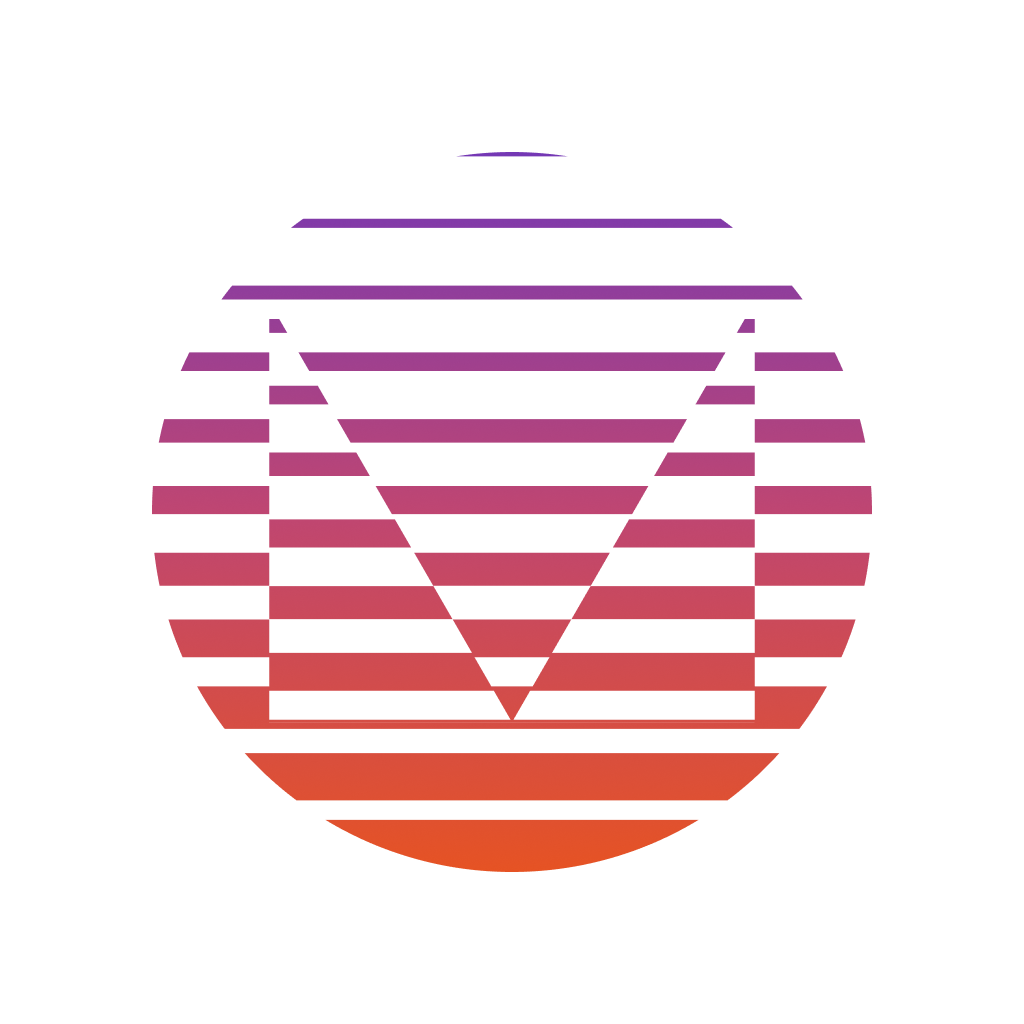
\includegraphics[height=7.5mm]{figures/openmathos-logo.png}};
  \node[anchor=west, text=covercream!72!coverindigo, font=\scriptsize, align=left]
    at ([xshift=-31mm,yshift=17mm]current page.south east)
    {Supported by\\[0.2mm] Open Math OS};

\end{tikzpicture}
\end{titlingpage}
\cleardoublepage

% Half-title: the title alone, on the first recto after the cover.
\thispagestyle{empty}
\vspace*{0.3\textheight}
\begin{center}{\LARGE\bfseries \hbtitle\par}\end{center}
\cleardoublepage

% Title page.
\begin{titlingpage}
\thispagestyle{empty}
\vspace*{0.12\textheight}
\begin{center}
{\color{hbblue}\fontsize{26}{32}\selectfont\bfseries \hbtitle\par}
\vspace{1.2em}{\color{hbgold}\rule{0.5\textwidth}{0.8pt}\par}\vspace{1.2em}
{\Large\itshape \hbsubtitle\par}
\vspace{0.12\textheight}
{\LARGE \hbauthor\par}\vspace{0.6em}
{\small \hbaffil\par}
\vfill
{\small \hbedition\\ Version \hbversion, \today\par}
\end{center}
\end{titlingpage}

% Imprint (copyright page), on the verso of the title page.
\thispagestyle{empty}
\vspace*{\fill}
\begin{flushleft}\small
\textbf{\hbtitle}\\
\hbsubtitle\\[1em]
\hbauthor\\
\hbaffil\\[1em]
\hbedition. Version \hbversion, compiled \today.\\
New papers are added each month from the zbMATH literature on derivations;
the list of changes is kept with the sources.\\[1em]
Mathematics Subject Classification (2020) % cite-ok: the MSC scheme names a classification, not a citable work
: 16W25, 17B40, 17A36, 13N15,
12H05, 46L57, 46H40, 47B47, 47L35, 16E40, 16S32, 13N10, 14R10, 17B66, 16R60.\\[1em]
ISBN: to be assigned.\\[1em]
\raisebox{-0.35em}{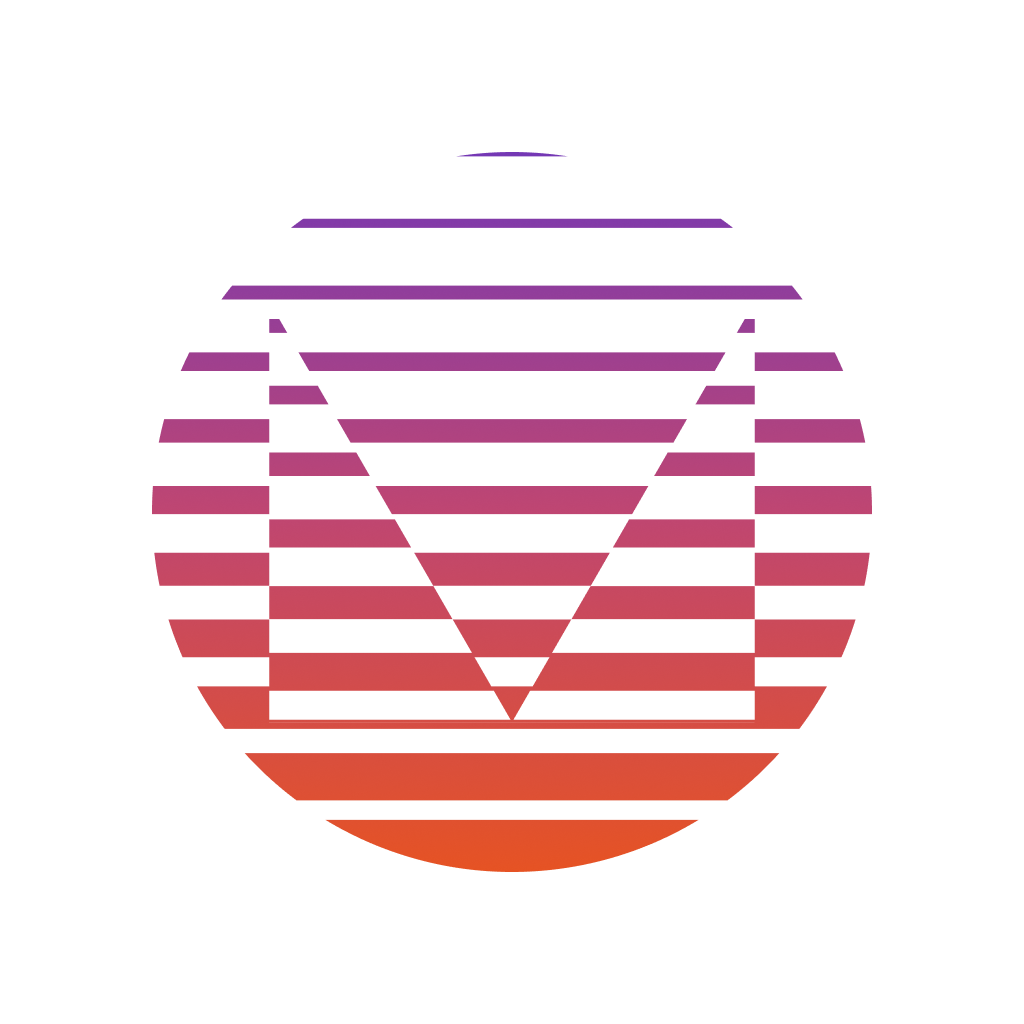
\includegraphics[height=1.7em]{figures/openmathos-logo.png}}\\[0.4em]
A encyclopaedia written in collaboration with AI.\\[1em]
\copyright\ 2026 \hbauthor. All rights reserved.
\end{flushleft}
\cleardoublepage

% Dedication.
% STATUS: written 2026-11-06 on the owner's instruction: the dedication is
% the Arabic phrase "إلى المستقبل" (to the future), and the words are the
% owner's, not the machine's. Corrected the same day: the first render had the
% two words in the wrong order, see below.
%
% The book is typeset with pdfLaTeX, which cannot set Arabic. ArabTeX is
% installed but sets its transliteration font with \it, which memoir rejects,
% and it does not take Unicode input. Rather than change the engine of a
% 392-page book for one line, the phrase is set once by XeLaTeX with the Amiri
% font and stored as figures/dedication-arabic.png.
%
% The bidi package matters here. XeLaTeX with fontspec alone shapes the Arabic
% letters correctly but lays the run out left to right, so the words came out
% in reverse order: the file was unreadable to an Arabic reader while looking
% plausible to anyone checking only the glyph shapes. The page must be
% typeset inside an Arabic environment from polyglossia (or with bidi), which
% is what orders the words right to left.
%
% Regenerate it with:
%   article class, geometry paper 120mm x 30mm margin 0, polyglossia with
%   \setmainlanguage{english} and \setotherlanguage{arabic},
%   \newfontfamily\arabicfont[Script=Arabic]{Amiri}, and in a centred body:
%     {\fontsize{40}{48}\selectfont\arabicfont
%      \begin{Arabic}إلى المستقبل\end{Arabic}}
%   xelatex, then pdftoppm -png -r 300, then trim the white margin and save
%   as figures/dedication-arabic.png.
\thispagestyle{empty}
\vspace*{0.28\textheight}
\begin{center}
  \includegraphics[width=0.34\textwidth]{dedication-arabic.png}
\end{center}
\cleardoublepage

% Contents, list of figures, list of tables.
\tableofcontents*
\cleardoublepage
\listoffigures*
\cleardoublepage
\listoftables*
\cleardoublepage

% Chapter contents: the index of the kinds of derivation-like map.
% out of the 200 rows the kind census holds (27 tokenizer fragments excluded).
% STATUS: written 2026-11-05 from ledger/encyclopaedia-kinds.tsv; corrected 2026-11-07;
% explanation of the counts and of the cut added 2026-11-09 (issue #1321).
% The mined TSV has 200 rows; 27 are tokenizer fragments and the 27 are in
% ledger/derivations-encyclopaedia-kinds-excluded.txt with their reason. The count of
% genuine kinds (count>=2) is the atlas's own, provenance `% ours: the numbered list
% of the atlas-mined kinds`. The genuine named kinds with a located citation
% (Weitzenb\"ock, Shamsuddin, Lotka--Volterra, triangular, Hasse--Schmidt, ...) are defined in their chapter.
% The number in parentheses after a name is the number of works in data/atlas.tsv whose
% title names that kind; it counts works, so it is unrelated to the number of chapters,
% sections or definitions. A title naming three kinds counts once under each of the three,
% so the numbers do not add up to a number of works. The list was cut at two works: a name
% on a single title in the whole atlas is not yet a kind the literature uses.
\chapter*{Index of the \textbf{173} kinds of derivation-like map}\label{page:index-of-kinds}
The titles of the works in the atlas name \textbf{173} kinds of derivation-like map,
out of the 200 rows the kind census holds. The 27 rows that are not kinds are
fragments of the mining method, and they are listed with their reason in the
book's kind ledger.
% ours: the numbered list below is the atlas-mined kinds
Each number after a name is the number of works whose title names that kind. A
title that names three kinds counts once under each of the three, so the numbers
do not add up to a number of works.
The list was cut at two works, because a name on a single title in the whole
atlas is not yet a kind the literature uses.
A name appears twice when the literature writes it two ways, joined by a dash and
written as one word: \emph{skew derivation} (179) with \emph{skew-derivation} (10), and
\emph{lie derivation} (107) with \emph{lie-derivation} (3). Each work counts once,
under the spelling its title uses.
The order is the order of the census table: by count, highest first. Kinds with
the same count are in the order the mining tool met them in the atlas, so the
order within a group of equal counts carries no meaning.

\begin{enumerate}
\item \allowbreak generalized derivation \hfill(592).
\item \allowbreak skew derivation \hfill(179).
\item \allowbreak higher derivation \hfill(145).
\item \allowbreak jordan derivation \hfill(135).
\item \allowbreak lie derivation \hfill(107).
\item \allowbreak triple derivation \hfill(98).
\item \allowbreak nilpotent derivation \hfill(85).
\item \allowbreak *-derivation \hfill(82).
\item \allowbreak local derivation \hfill(80).
\item \allowbreak 2-local derivation \hfill(75).
\item \allowbreak ($\alpha$, $\beta$)-derivation \hfill(68).
\item \allowbreak n-derivation \hfill(68).
\item \allowbreak ($\sigma$, $\tau$)-derivation \hfill(67).
\item \allowbreak inner derivation \hfill(66).
\item \allowbreak left derivation \hfill(62).
\item \allowbreak unbounded derivation \hfill(34).
\item \allowbreak symmetric bi-derivation \hfill(30).
\item \allowbreak f-derivation \hfill(30).
\item \allowbreak multiplicative derivation \hfill(23).
\item \allowbreak b-generalized derivation \hfill(23).
\item \allowbreak superderivation \hfill(22).
\item \allowbreak ternary derivation \hfill(22).
\item \allowbreak ($\theta$, $\phi$)-derivation \hfill(21).
\item \allowbreak simple derivation \hfill(20).
\item \allowbreak reverse derivation \hfill(20).
\item \allowbreak (generalized)-derivation \hfill(20).
\item \allowbreak lie-type derivation \hfill(19).
\item \allowbreak outer derivation \hfill(18).
\item \allowbreak semiderivation \hfill(18).
\item \allowbreak hasse-schmidt derivation \hfill(13).
\item \allowbreak algebraic derivation \hfill(12).
\item \allowbreak additive derivation \hfill(12).
\item \allowbreak polynomial derivation \hfill(12).
\item \allowbreak monomial derivation \hfill(12).
\item \allowbreak k-derivation \hfill(12).
\item \allowbreak generic derivation \hfill(12).
\item \allowbreak normal derivation \hfill(11).
\item \allowbreak linear derivation \hfill(11).
\item \allowbreak commuting derivation \hfill(11).
\item \allowbreak double derivation \hfill(11).
\item \allowbreak integrable derivation \hfill(10).
\item \allowbreak quadratic derivation \hfill(10).
\item \allowbreak bi-derivation \hfill(10).
\item \allowbreak (f, g)-derivation \hfill(10).
\item \allowbreak generalized semiderivation \hfill(10).
\item \allowbreak skew-derivation \hfill(10).
\item \allowbreak module derivation \hfill(9).
\item \allowbreak closed derivation \hfill(9).
\item \allowbreak order derivation \hfill(9).
\item \allowbreak positive derivation \hfill(9).
\item \allowbreak twisted derivation \hfill(9).
\item \allowbreak (m, n)-jordan derivation \hfill(9).
\item \allowbreak hom-derivation \hfill(9).
\item \allowbreak point derivation \hfill(8).
\item \allowbreak finite derivation \hfill(8).
\item \allowbreak vanishing derivation \hfill(8).
\item \allowbreak ($\alpha$, $\alpha$)-derivation \hfill(8).
\item \allowbreak permuting tri-derivation \hfill(8).
\item \allowbreak local superderivation \hfill(8).
\item \allowbreak (m, n)-derivation \hfill(8).
\item \allowbreak nonsingular derivation \hfill(7).
\item \allowbreak q-skew derivation \hfill(7).
\item \allowbreak quasi-derivation \hfill(7).
\item \allowbreak weitzenb\"ock derivation \hfill(7).
\item \allowbreak central derivation \hfill(7).
\item \allowbreak 3-derivation \hfill(7).
\item \allowbreak ($\alpha$, $\beta$, $\gamma$)-derivation \hfill(7).
\item \allowbreak p-derivation \hfill(7).
\item \allowbreak random derivation \hfill(6).
\item \allowbreak triangular derivation \hfill(6).
\item \allowbreak t-derivation \hfill(6).
\item \allowbreak jordan superderivation \hfill(6).
\item \allowbreak approximate derivation \hfill(6).
\item \allowbreak continuous derivation \hfill(6).
\item \allowbreak right derivation \hfill(6).
\item \allowbreak 2-local superderivation \hfill(6).
\item \allowbreak m-derivation \hfill(6).
\item \allowbreak coderivation \hfill(5).
\item \allowbreak homo-derivation \hfill(5).
\item \allowbreak super-derivation \hfill(5).
\item \allowbreak ($\sigma$, $\tau$)-higher derivation \hfill(5).
\item \allowbreak conformal derivation \hfill(5).
\item \allowbreak $\sigma$-derivation \hfill(5).
\item \allowbreak g-derivation \hfill(5).
\item \allowbreak anti-derivation \hfill(5).
\item \allowbreak jordan-type derivation \hfill(5).
\item \allowbreak bi-semiderivation \hfill(5).
\item \allowbreak elementary derivation \hfill(4).
\item \allowbreak semisimple derivation \hfill(4).
\item \allowbreak ($\theta$, $\theta$)-derivation \hfill(4).
\item \allowbreak generalised derivation \hfill(4).
\item \allowbreak bounded derivation \hfill(4).
\item \allowbreak ($\phi$, $\psi$)-derivation \hfill(4).
\item \allowbreak symplectic derivation \hfill(4).
\item \allowbreak partial derivation \hfill(4).
\item \allowbreak r-derivation \hfill(4).
\item \allowbreak ($\sigma$, $\tau$, $\xi$)-derivation \hfill(4).
\item \allowbreak jacobian derivation \hfill(4).
\item \allowbreak preserving derivation \hfill(4).
\item \allowbreak n-higher derivation \hfill(4).
\item \allowbreak *-lie derivation \hfill(4).
\item \allowbreak universal derivation \hfill(3).
\item \allowbreak self-adjoint derivation \hfill(3).
\item \allowbreak homogeneous derivation \hfill(3).
\item \allowbreak gamma-derivation \hfill(3).
\item \allowbreak locally-finite derivation \hfill(3).
\item \allowbreak abstract derivation \hfill(3).
\item \allowbreak higher-order derivation \hfill(3).
\item \allowbreak hyponormal derivation \hfill(3).
\item \allowbreak quasi-free derivation \hfill(3).
\item \allowbreak compact derivation \hfill(3).
\item \allowbreak braided derivation \hfill(3).
\item \allowbreak factorizable derivation \hfill(3).
\item \allowbreak shamsuddin derivation \hfill(3).
\item \allowbreak orthogonal derivation \hfill(3).
\item \allowbreak multi-derivation \hfill(3).
\item \allowbreak zero derivation \hfill(3).
\item \allowbreak symmetric derivation \hfill(3).
\item \allowbreak logarithmic derivation \hfill(3).
\item \allowbreak m-integrable derivation \hfill(3).
\item \allowbreak *-double derivation \hfill(3).
\item \allowbreak left bi-derivation \hfill(3).
\item \allowbreak combinatorial derivation \hfill(3).
\item \allowbreak cubic derivation \hfill(3).
\item \allowbreak cyclotomic derivation \hfill(3).
\item \allowbreak lie superderivation \hfill(3).
\item \allowbreak $\alpha$-generalized derivation \hfill(3).
\item \allowbreak (generalized)-skew derivation \hfill(3).
\item \allowbreak multiplicative semiderivation \hfill(3).
\item \allowbreak lie-derivation \hfill(3).
\item \allowbreak ($\alpha$, $\beta$)-reverse derivation \hfill(3).
\item \allowbreak $\theta$-derivation \hfill(3).
\item \allowbreak nil derivation \hfill(2).
\item \allowbreak stable derivation \hfill(2).
\item \allowbreak hypercentral derivation \hfill(2).
\item \allowbreak bilocal derivation \hfill(2).
\item \allowbreak weight derivation \hfill(2).
\item \allowbreak diagonalizable derivation \hfill(2).
\item \allowbreak d-derivation \hfill(2).
\item \allowbreak peirce derivation \hfill(2).
\item \allowbreak odd derivation \hfill(2).
\item \allowbreak reducible derivation \hfill(2).
\item \allowbreak closable derivation \hfill(2).
\item \allowbreak noncommuting derivation \hfill(2).
\item \allowbreak constant-free derivation \hfill(2).
\item \allowbreak integral derivation \hfill(2).
\item \allowbreak near-derivation \hfill(2).
\item \allowbreak extended derivation \hfill(2).
\item \allowbreak ($\alpha$, $\beta$)-higher derivation \hfill(2).
\item \allowbreak quartic derivation \hfill(2).
\item \allowbreak b-derivation \hfill(2).
\item \allowbreak f bi-derivation \hfill(2).
\item \allowbreak volterra derivation \hfill(2).
\item \allowbreak jordan-triple derivation \hfill(2).
\item \allowbreak generalized coderivation \hfill(2).
\item \allowbreak ternary bi-derivation \hfill(2).
\item \allowbreak ($\alpha$, $\beta$)-generalized derivation \hfill(2).
\item \allowbreak leibniz-derivation \hfill(2).
\item \allowbreak generalized superderivation \hfill(2).
\item \allowbreak graded derivation \hfill(2).
\item \allowbreak weak-local derivation \hfill(2).
\item \allowbreak lotka-volterra derivation \hfill(2).
\item \allowbreak modular derivation \hfill(2).
\item \allowbreak e-derivation \hfill(2).
\item \allowbreak generalized semi-derivation \hfill(2).
\item \allowbreak poisson derivation \hfill(2).
\item \allowbreak involutive derivation \hfill(2).
\item \allowbreak fuzzy derivation \hfill(2).
\item \allowbreak schmidt derivation \hfill(2).
\item \allowbreak n-lie derivation \hfill(2).
\item \allowbreak generalized bi-derivation \hfill(2).
\item \allowbreak bracket derivation \hfill(2).
\item \allowbreak *-reverse derivation \hfill(2).
\end{enumerate}

\chapter*{Preface}
\addcontentsline{toc}{chapter}{Preface}
% STATUS: written 2026-11-06 (states the scope, the source rule and the living
% edition rule; these are the book's own policies, fixed in CLAUDE.md and in the
% ROADMAP, not external claims.)
\label{page:preface}

A derivation is the algebraic form of a derivative.
Leibniz wrote the product rule in 1684, and three centuries later the same rule
defines a map on any ring: an additive map $d$ with $d(xy)=d(x)y+xd(y)$.
Every chapter of this book studies some version of that equation, either the
equation itself or a weaker or stronger form of it.

\section*{Why a encyclopaedia and not a survey}

A survey selects and argues. A encyclopaedia tries to be complete in scope, so that a
reader can find where a given question is treated and what is known about it.

This book is exhaustive in scope, not in text.
Every flavour of derivation, every class of ring and algebra where derivations
act, and every line of development from Leibniz to this year has a place in the
plan.
The plan is fixed in advance and the text grows into it.

\section*{The source rule}

No fact, definition, example or application is stated before its source has been
read in full from the page.
A recalled theorem appears as a theorem-like environment with its located
citation, keeping the kind and the wording of the source.
Proofs and remarks of the book itself are marked as its own.

This rule has a cost, and the cost is visible.
A section whose sources are not yet obtained stays a marked planned
stub, and the stub says which source it waits for.
A reader who finds a stub knows that the coverage is planned there.
The text is not yet written, which is a different thing from a section that was
written and then cut.

This edition has no such stub.
Every section is written.
Some sources cited in the bibliography could not be opened at all.
Their entries carry the marker `unverified-ref` together with the reason, and
their sections cite them for what the record states rather than quoting a
theorem from a page nobody has seen.
The count is kept in the download record of this book, not here, because it
changes as copies are found.
The work list that the search step keeps records the same fact for the works
that were found and not cited: a lead is not a source until its page has been
read.
The policy stays in place for later editions, which is why it is stated here.

\section*{Where the applications are}

A derivation is a rule that obeys the Leibniz product rule. The rule itself
goes back to Leibniz \cite{Leibniz1684}. The name was already familiar to
Ritt when he built differential algebra on it \cite[p.~1]{Ritt1950}. The same
rule appears again in nine fields beyond the differential calculus. The nine
names are classical and quantum mechanics, differential geometry,
differential algebra, coding, control, group analysis, model theory,
algebraic topology and automatic differentiation. Each field is reported in
the chapter that owns its notions.
Each report names one field, cites the source that names the derivation it
rests on, and reads the definition or theorem of that source. The reports do
not narrate: they record.

Physics was the first field that asked why a derivation arises. Dirac
\cite{Dirac1925} translated noncommutative kinematics into the language of a
Poisson bracket
(Section~\ref{sec:basic-theory:physics}), and Kadison \cite{Kadison1966} later
asked whether every derivation of an operator algebra comes from inside
(Section~\ref{sec:banach-operator:kadison-sakai}). Geometry came next: a tangent vector
at a point of a smooth manifold is a derivation of the smooth functions there
(Section~\ref{sec:commutative:geometry}). Differential algebra began when Ritt
and Kolchin axiomatized the symbol $d/dx$ as a derivation on a field, and the
field-of-definition question for the Painlev\'e equations sits inside that
axiomatization (Section~\ref{sec:differential-algebra:differential-equations}). In
positive characteristic the ordinary product rule survives in the
divided-power form of Hasse and Schmidt; the higher derivations are the
algebraic backbone of Reed--Solomon and Goppa codes
(Section~\ref{sec:higher-multi:coding}). Control theory discovered that an
input--output system is a finitely generated differential field extension,
with the input a differential transcendence basis
(Section~\ref{sec:differential-algebra:control}). On a group the same rule is a
derivation of the group ring, and Fox showed the free group carries one
derivation per generator (Section~\ref{sec:group-hopf:harmonic-analysis}).
Ax translated the conjecture of Schanuel about the complex exponential into a
statement about a derivation on a differential field. His 1971 theorem is the
seed of the Ax--Schanuel inequalities
(Section~\ref{sec:differential-algebra:transcendence}). Hochschild and cyclic
homology compute derivations as the homology of a chain complex, and on a
smooth commutative algebra the answer is the exterior algebra of K\"ahler
differentials (Section~\ref{sec:cohomology:algebraic-topology}). A computer
program that differentiates a function runs the chain rule and the Leibniz
rule step by step under automatic differentiation
(Section~\ref{sec:differential-algebra:automatic-differentiation}).

\hbfigure{02-basic-theory/oscillator}{The harmonic oscillator. The derivation $f\mapsto\{f,H\}$ with $H=(p^2+q^2)/2$ is the vector field $(p,-q)$ on the phase plane; its flow is a rotation.}{fig:basic:oscillator}

\section*{The living edition}

The subject grows.
Papers on derivations appear every month, and a printed encyclopaedia would be out of
date before it reached a reader.
This edition is therefore updated monthly: new work is added where it changes a
statement, a table entry or an open problem.
Appendix~\ref{app:atlas} reports what the edition has read, and the version
number on the title page names the edition.

\section*{How the book was made}

The work of reading, checking and drafting was carried out with artificial
intelligence under human direction.
A person set the scope, fixed the questions and decided what the book would
contain.
Machine tools assisted the reading of each source, the extraction of its results
and the drafting of each section.
Every claim was then checked against the page it cites.
The rules that govern this are stated in the repository of the book.
The records of what was read are kept there too, so a reader can trace any
statement to its source.

The name on the title page is the person who directed the work and answers for
it.

\chapter*{How to use this encyclopaedia}
\addcontentsline{toc}{chapter}{How to use this encyclopaedia}
% STATUS: written 2026-11-06 (describes the organisation the book already has:
% the eight question families of Section~\ref{sec:basic-theory:question-families},
% the chapter layout, and the two appendices. No new claim is made.)
\label{page:how-to-use}

The book is organised around eight questions, not around its chapters.
A reader who wants one of them answered can go straight to the
appendix that indexes it. A reader who wants to follow the subject from its
beginnings can read Part~I onward.

\section*{The eight question families}

Section~\ref{sec:basic-theory:question-families} fixes the eight questions the
book asks of every class of algebra. They are:

\begin{enumerate}
\item Which kind of derivation implies which other?
\item When are two definitions equivalent?
\item Is every derivation inner?
\item Is every derivation continuous, and does continuity come for free?
\item Does the algebra have to be commutative?
\item Can all derivations of the class be described?
\item Does a derivation extend or lift to a larger algebra?
\item Where does an expected implication fail?
\end{enumerate}

The chapters answer them in this order wherever the sources allow.
Appendix~\ref{app:questions} collects the answers in tables, family by family,
so that a reader comparing two classes of algebra can see both at once.

\section*{How a chapter is laid out}

Each chapter follows the same plan.

The introduction gives the history: why the topic arose, who first asked the
question, and what the chapter answers.
The sections that follow begin with the definitions as their sources state them,
then the theorems as their sources state them, each with the page or numbered
item.

Counterexamples come where a family of the last kind fails; they are what
answers family~8.
An application comes where the notion it uses is defined, so the reader meets
the use at the same point as the idea.
An open problem comes where the chapter states the question it belongs to,
and Appendix~\ref{app:questions} gathers all of them by family and by class.

A recalled theorem keeps the kind of its source: a proposition stays a
proposition, and a theorem stays a theorem.
The book never states a recalled result again in its own setting.
The specialisation is written after the recall, and it refers to the recall by
number.

\section*{The two appendix chapters}

Appendix~\ref{app:atlas} is the atlas of the literature.
It gives the shape of the bibliography: the works by decade, by language, and by
the kind of derivation-like map they treat.
It is counted again with each edition, so it records what this edition has read
rather than what the field contains.

Appendix~\ref{app:questions} is the collection of question tables.
For each of the eight families it gives, class by class, whether the answer is
known, false with a counterexample, or open, with the source that settles or
asks it.

\section*{Reading paths}

A reader new to the subject can read Part~I in order; it carries the history and
the basic theory, and it fixes the question families.
A reader who works on rings can take Part~II and Part~III, which treat the
associative classes, and consult Part~VI for the analytic ones.
A reader who comes from analysis or operator theory can start with Part~VI and
use Part~II for the algebraic background.
A reader who wants the current frontier can read
Appendix~\ref{app:questions}, which names every open problem with the chapter
that states it, then follow those references back.

\section*{The living edition}

The edition is updated each month.
New work is added where it changes a statement, a table entry or an open
problem.
A work that only confirms what the book already says is not cited for that
alone.
The version number appears on the title page, so that a citation to this book
can name the edition it used.

\chapter*{Notation and conventions}
\addcontentsline{toc}{chapter}{Notation and conventions}
% STATUS: written 2026-11-06 (records the notations the chapters actually use;
% each symbol is defined in its chapter, and this list is the index to them.
% Operators come from style/encyclopaedia.sty; no new notation is introduced here.)
\label{page:notation}

The book keeps one notation throughout.
A symbol is defined where it first appears, and the chapters reuse it without
giving it a second meaning.
This page lists the symbols a reader meets most often, so that a chapter can be
opened at any point.

\section*{Rings and algebras}

$R$ and $A$ are a ring and an algebra; the book says which when the distinction
matters. $\mathbb{F}$ is a field, and $k$ is a field when the work is
geometric. $\operatorname{char}R$ is the characteristic of $R$, and $Z(R)$ is
its centre.
An algebra is associative and unital unless a chapter says otherwise;
Chapter~\ref{ch:nonassociative} drops associativity and says so at each step.

$M_n(R)$ is the ring of $n\times n$ matrices over $R$.
A triangular algebra is written $A=\operatorname{Tri}(A_1,A_2,M)$ with $M$ the
bimodule between the two parts.
$R[x]$ and $R[x_1,\dots,x_n]$ are polynomial rings, and $k(x)$ is the field of
fractions when $k$ is a domain.

\section*{Derivations and their relatives}

$\operatorname{Der}(A)$ is the set of derivations of $A$, an additive group and
a Lie algebra under the commutator.
$\operatorname{Inn}(A)$ is the set of inner derivations, those of the form
$x\mapsto[\,a,x\,]$, so that
$\operatorname{HH}^{1}(A,A)\cong\operatorname{Der}(A)/\operatorname{Inn}(A)$ for
the classes where that identification holds.

$\operatorname{JDer}(A)$ and $\operatorname{LDer}(A)$ are the Jordan and the Lie
derivations. $\operatorname{ad}_a$ is the inner derivation $x\mapsto[a,x]$.
A derivation is \emph{locally nilpotent} when some power of it kills each
element, and the set of these is written $\operatorname{LND}(A)$. % ours: notation-page term, defined in Chapter 16

$\operatorname{HH}^{\bullet}(A,M)$ is the Hochschild cohomology of $A$ with
coefficients in the bimodule $M$, and $\operatorname{HH}^{\bullet}(A)$ is the
case $M=A$.
Low degrees are written out where they are used: the first cohomology group is
the derivations modulo the inner ones.

\section*{Maps and products}

$[x,y]=xy-yx$ is the commutator and $x\circ y=xy+yx$ is the anti-commutator.
A map is \emph{additive} when it respects addition, with no linearity assumed
over a ring; the book states linearity separately wherever a theorem needs it. % ours: notation-page convention

For maps with a parameter, $\sigma$ and $\tau$ are endomorphisms of the algebra,
and $\alpha$, $\beta$ are scalars or endomorphisms as the chapter says.
A $\sigma$-derivation satisfies $d(xy)=d(x)y+\sigma(x)d(y)$, and the book gives
the defining identity for each twisted kind at the point where it is named.

\section*{Continuity and operators}

For a Banach algebra, $\lVert\cdot\rVert$ is the norm, and a derivation is
\emph{bounded} when it is bounded as a linear map. % ours: notation-page term, defined in Chapter 18
The book asks, for each class, whether continuity has to be assumed or comes for
free; the question is fixed in
Section~\ref{sec:basic-theory:question-families} and answered by class in the
chapters.

$\mathcal{B}(H)$ is the algebra of bounded operators on a Hilbert space $H$, and
$\mathcal{K}(H)$ is the ideal of compact operators.
A von Neumann algebra is written $M$.

\section*{Conventions}

A theorem recalled from a source carries the source in its header, with the page
or the numbered item.
A result proved in this book is marked as one of its own.
A citation after a sentence gives the page on which the cited source says what
the sentence attributes to it.

The book uses British spelling in the text and keeps the spelling of a quoted
title.
Section and theorem numbers are stable within an edition; a later edition may
add a section at the end of a chapter, which leaves earlier numbers alone.


\mainmatter
% Generated by tools/scripts/encyclopaedia/build-tree.sh from structure.txt.
% Do not edit: change structure.txt and rerun.
\part{Foundations and history}
% Generated by tools/scripts/encyclopaedia/build-tree.sh from structure.txt.
% MSC codes feeding this chapter: 12H05 13N15 16E40 17B40 20J06
\chapter{Origins of the notion, from Leibniz to Hochschild}\label{ch:origins}
% Chapter introduction: why the topic arose, who first asked, what it answers.
% STATUS: written 2026-11-06 (English gate clean; sources read in full as recorded below).
% Summarises Sections 1--10 of this chapter; every claim is cited in its section.

A derivation of an algebra $A$ is a linear map $D\colon A \to A$ with
\[
  D(xy) = D(x)\,y + x\,D(y).
\]
The definition is short, but it came late. The product rule is as old as the
calculus. For two and a half centuries it was only a property of the
derivative of a function. It became a definition only in the 1920s and 1930s.
Then a derivation became a map on an abstract algebra, fixed by this one
identity.

This chapter tells how that happened. The story has three parts, and
Figure~\ref{fig:origins:timeline} places its sources in time. We use modern
notation throughout. $A$ is an algebra, $M$ a bimodule, $K$ and $k$ are fields,
and $G$ is a group. Maps are written on the left. When a source uses other
notation, we say so once.

\hbfigure{01-origins/timeline}{The sources of Chapter~1 in order of publication.}{fig:origins:timeline}

The first part stays with commutative rings and fields. It starts in 1684,
when Leibniz states the product rule for his differences
(Section~\ref{sec:origins:leibniz-rule}). Two centuries later, Dedekind and
Weber need a derivative of algebraic functions without any limits. In 1882
they define it by algebra alone, and in 1897 Hilbert writes the different of
an algebraic number as a derivative (Section~\ref{sec:origins:function-fields}).

In characteristic $p$ there is a new difficulty. A nonzero polynomial can
have zero derivative; for example, $x^p$ does
\cite[\S 9, p.~213]{Steinitz1910}. Steinitz
meets this in 1910. Later it leads Jacobson to a Galois theory in which
derivations take the place of automorphisms
(Section~\ref{sec:origins:fields-and-separability}). It also leads Hasse and
Schmidt to higher derivations (Section~\ref{sec:origins:higher-derivations}).
Meanwhile Ritt and his students study fields with a derivation. For them such
a field is the natural setting for differential equations
(Section~\ref{sec:origins:differential-algebra}).

The second part leaves commutativity behind. In 1925 Born and Jordan keep the
product rule for matrices. In the same year Dirac shows that every such
operation on quantum variables is a commutator
(Section~\ref{sec:origins:physics}). In 1933 Ore builds polynomials over a
skew field. He finds a product rule twisted by an endomorphism
(Section~\ref{sec:origins:ore-and-twists}). In 1937 Jacobson studies the
derivations of any algebra. He shows that they form a Lie algebra, and in
characteristic $p$ a restricted one (Section~\ref{sec:origins:lie-theory}).

The third part shows how these lines meet. Since Hilbert, number theorists
had studied maps called crossed homomorphisms. They come from groups that act
on fields (Section~\ref{sec:origins:crossed-homomorphisms}). In 1945
Hochschild puts the derivations of an algebra into a cohomology theory.
Derivations are the one-cocycles, and inner derivations are the coboundaries
(Section~\ref{sec:origins:cohomology}). After this step the derivation is a
central object of modern algebra.

Along the way, three facts appear again and again. They are also the first
questions of the rest of the book.

The first fact concerns constants. A derivation is fixed by one identity, and
its kernel is the set of constants. This kernel carries information about the
algebra. Automorphisms have fixed points in the same way. Dedekind, Weber,
Steinitz and Jacobson all use this link
(Sections~\ref{sec:origins:function-fields}
and~\ref{sec:origins:fields-and-separability}).

The second fact concerns brackets. The commutator of two derivations is again
a derivation. So the derivations of any algebra form a Lie algebra. Dirac
meets this fact in physics, and Jacobson makes it the base of a theory
(Sections~\ref{sec:origins:physics} and~\ref{sec:origins:lie-theory}).

The third fact concerns inner derivations. For every element $a$, the map
$x \mapsto ax - xa$ is a derivation. When does every derivation have this
form? Dirac asked this for matrices. Hochschild answered it in general with
the group $H^1$ (Sections~\ref{sec:origins:crossed-homomorphisms}
and~\ref{sec:origins:cohomology}). The question runs through every later
chapter.

% STATUS: written 2026-11-06 (English gate clean; sources read in full as recorded below).
% Sources read in full: Leibniz 1684 (Acta Eruditorum, October 1684, 467--473; scan archive.org s1id13206500, rules of the calculus on p. 467 checked in the OCR text), Jacobson 1937 (Amer. J. Math. 59, 205--220; the definition (2c) on p. 206).
\section[The Leibniz rule: Leibniz 1684][The Leibniz rule]{The Leibniz rule: Leibniz 1684}\label{sec:origins:leibniz-rule}

Every derivation in this book satisfies the same identity:
\[
  D(xy) = D(x)\,y + x\,D(y).
\]
This rule first appears in print in a paper of Leibniz of October
1684~\cite{Leibniz1684}. The paper is written in Latin. It is the paper that
introduced the differential calculus.

Why did Leibniz need such a rule? The title of the paper names the problem. Leibniz wants a method for maxima,
minima and tangents \translated{which is not stopped by fractions or by
irrational quantities}{quae nec fractas nec irrationales quantitates
moratur}{Latin}. The
methods of his time first removed all square roots from an equation. Leibniz
describes this work as follows:
\begin{originalquote}{Latin}{calculo praestare sublatis irrationalibus, taediosissimae et aliquando insuperabilis operae}
to carry out by calculation after removing the irrationals, a most tedious
and sometimes insuperable labour
\end{originalquote}
\noindent\cite[p.~472]{Leibniz1684}. His answer is a set of rules. Each rule
acts on one symbol of a formula at a time. So a square root or a fraction
needs no preparation. He tests the rules on the law of refraction, which he
finds as a minimum. Then he remarks~\cite[p.~472]{Leibniz1684}:
\begin{originalquote}{Latin}{Cum alii doctissimi Viri multis ambagibus venati sint, quae hujus calculi peritus tribus lineis imposterum praestabit.}
Whereas other most learned men have hunted with many detours for what one
skilled in this calculus will henceforth achieve in three lines.
\end{originalquote}
\noindent The product rule is one of these rules. It gives the differential of
a product from the differentials of its factors. Nothing has to be expanded.

To define his differences, Leibniz draws a curve above a horizontal axis. A point $X$ on the axis has
abscissa $x$, and the curve has height $v$ above it. The tangent to the curve
at that point meets the axis at a point $B$. The segment $BX$ is called the
\emph{subtangent} \cite[p.~467]{Leibniz1684}. Leibniz chooses any segment $dx$. Then he defines $dv$ by
the proportion
\[
  dv : dx = v : BX .
\]
He calls $dv$ the \emph{differentia}, that is, the difference of $v$ \cite[p.~467]{Leibniz1684}.
Figure~\ref{fig:origins:subtangent} shows the construction.

\hbfigure{01-origins/leibniz-subtangent}{The construction of Leibniz \cite[p.~467]{Leibniz1684}. The tangent at $V$ meets the axis at $B$, and $BX$ is the subtangent. The difference $dv$ satisfies $dv : dx = v : BX$.}{fig:origins:subtangent}

With this construction, Leibniz states his rules. The first two rules say that constants have zero difference and that $d$ is
linear: \translated{Let $a$ be a given constant quantity; then $da$ will be
equal to $0$, and $d\,ax$ will be equal to $a\,dx$}{Sit $a$ quantitas data
constans, erit $da$ aequalis $0$, \& $d\,ax$ erit aequ.\ $a\,dx$}{Latin}. The
difference of a sum is the sum of the differences. The third rule is the
product rule: \translated{Multiplication: $d\,xv$ equals $x\,dv +
v\,dx$}{Multiplicatio, $d\,xv$ aequ.\ $x\,dv + v\,dx$}{Latin}%
~\cite[p.~467]{Leibniz1684}. The quotient rule follows on the same page.
Figure~\ref{fig:origins:product-area} gives the usual picture of the product
rule.

\hbfigure{01-origins/product-rule-area}{The product rule read as area. When $x$ and $v$ grow by $dx$ and $dv$, the rectangle $xv$ grows by $x\,dv + v\,dx$. The small corner $dx\,dv$ is of higher order.}{fig:origins:product-area}

Three features of this passage return in every later definition. First, the
rules are stated for symbols, and no limit appears. Leibniz says that $dx$ is
treated in the calculus like $y$ and $dy$, or like any other letter with its
differential~\cite[p.~467]{Leibniz1684}.

Second, constants are exactly the quantities that $d$ sends to zero. Dedekind
and Weber stress the same property two centuries later
(Section~\ref{sec:origins:function-fields}). Third, the product rule is the
only rule that links $d$ to multiplication. So a linear map with this rule
behaves like a derivative in every computation made of sums and products.

Today the third feature is the definition itself. Let $k$ be a commutative ring and $A$ a $k$-algebra. A \emph{derivation} of
$A$ is a $k$-linear map $D\colon A \to A$ with $D(xy) = D(x)y + xD(y)$ for all
$x, y \in A$ \cite[p.~206]{Jacobson1937}. If $A$ has a unit, then $D(1) = D(1\cdot 1) = 2D(1)$, so
$D(1) = 0$. By linearity, $D$ vanishes on the image of $k$. Induction on the
product rule gives the general Leibniz formula:
\[
  D^n(xy) = \sum_{i=0}^{n} \binom{n}{i} D^i(x)\, D^{n-i}(y).
\]
Jacobson uses this formula in 1937. It shows that in characteristic $p$ the
$p$-th power of a derivation is again a derivation
(Section~\ref{sec:origins:lie-theory}). Chapter~\ref{ch:basic-theory}
develops the definition and its first consequences.

For two centuries after Leibniz, the product rule stayed a rule of analysis.
It entered algebra through the theory of algebraic functions, as the next
section shows.

% STATUS: written 2026-11-06 (English gate clean; sources read in full as recorded below).
% Sources read in full: Dedekind--Weber 1882 (J. reine angew. Math. 92, 181--290; scan archive.org journalfrdierei42crelgoog, Sections 11 and 23 and the plan on p. 183 checked in the OCR text; Section 23, headed "Die Differentialquotienten", opens on p. 259), Hilbert 1897 (Jahresber. DMV 4, Section 3 checked against the page image, p. 179, where the Differente is defined), Hecke 1923 (Section 36, OCR text).
% Not yet read: Hensel--Landsberg 1902; Kronecker 1882 (Grundzuege, same volume 92, pp. 1--122).
\section[Differentiation in number and function fields: Dedekind, Weber, Hensel, Hilbert][Number and function fields]{Differentiation in number and function fields: Dedekind, Weber, Hensel, Hilbert}\label{sec:origins:function-fields}

The derivative of a polynomial did algebraic work long before derivations
were defined on rings. It did this work in two places. The first place is
the theory of algebraic functions of one variable. The second place is the
arithmetic of number fields.

Riemann defined differentials on a Riemann surface by analysis. Dedekind and
Weber wanted the same objects without any use of continuity. In number
fields, the derivative of a defining polynomial gives a number called the
\emph{different}~\cite[\S 3, p.~179]{Hilbert1897}. It is defined through the derivative.

Dedekind and Weber gave an answer in 1882. Their memoir is \emph{Theorie der algebraischen Functionen einer
Ver\"anderlichen}~\cite{DedekindWeber1882}. It is written in German. It
builds the theory of Riemann surfaces again, from the arithmetic of ideals. The
introduction states the plan: \translated{A formal definition of the
differential quotient based on this then leads to the genus and to a
completely general, elegant representation of the differentials of the first
kind}{Eine darauf gegr\"undete formale Definition des Differentialquotienten
f\"uhrt sodann zu der Geschlechtszahl und zu einer ganz allgemeinen,
eleganten Darstellung der Differentiale erster Gattung}{German}%
~\cite[p.~183]{DedekindWeber1882}. The same page adds a remark. Up to the
Riemann--Roch theorem, continuity and power series play no role.

The definition is in Section~23, \emph{Die Differentialquotienten}
\cite[\S 23, p.~259]{DedekindWeber1882}. We
follow it in our translation. Let $\Omega$ be the field of algebraic
functions. Let $\alpha$ and $\beta$ be elements of $\Omega$. Assume that
$\beta$ is not constant. The two elements satisfy an irreducible equation
$F(\alpha,\beta) = 0$. Dedekind and Weber show that $\Omega$ contains a
function $(d\alpha/d\beta)$. At almost every point, its value is the limit of
the difference quotient. A footnote gives a purely algebraic formula:
\[
  \Bigl(\frac{d\alpha}{d\beta}\Bigr) = -\,\frac{F'(\beta)}{F'(\alpha)}.
\]
Here $F'(\alpha)$ and $F'(\beta)$ are the two partial derivatives of~$F$.
With this formula they prove the chain rule:
\[
  \frac{d\alpha}{d\beta} = \frac{d\alpha}{d\gamma}\,\frac{d\gamma}{d\beta}
\]
\cite[\S 23, pp.~259--260]{DedekindWeber1882}. Next they give every element
$\alpha$ a differential $d\alpha$. It satisfies $d\alpha =
(d\alpha/d\beta)\, d\beta$. They note that \translated{the differentials of the
constants, and only these, are to be set equal to zero}{Die Differentiale der
Constanten, und nur diese sind Null zu setzen}{German}. Finally, take any
rational relation $F(\alpha,\beta,\gamma,\ldots) = 0$. From it they derive
$F'(\alpha)\,d\alpha + F'(\beta)\,d\beta + F'(\gamma)\,d\gamma + \cdots = 0$%
~\cite[\S 23, p.~261]{DedekindWeber1882}.

In modern language, the construction reads as follows. Fix a nonconstant element $z$. Then the map $\alpha \mapsto d\alpha/dz$ is a
derivation of $\Omega$. Its kernel is exactly the field of constants. The map
$\alpha \mapsto d\alpha$ is an early form of the universal derivation
(Section~\ref{sec:commutative:kahler}). Dedekind and Weber did not use these
words. They needed a derivative defined by algebra alone. With it, they
reached the genus and the differentials of the first kind without analysis.

On the side of arithmetic, the derivative appears in the \emph{Zahlbericht} of Hilbert~\cite{Hilbert1897}. It is written in German.
Let $\alpha$ be an algebraic number. Let $\alpha', \ldots, \alpha^{(m-1)}$ be
its conjugates. Hilbert calls the product
\[
  \delta(\alpha) = (\alpha-\alpha')(\alpha-\alpha'')\cdots(\alpha-\alpha^{(m-1)})
\]
the \emph{different} of~$\alpha$. He notes that it is again a number of the
field. Indeed, put $f(x) = (x-\alpha)(x-\alpha')\cdots(x-\alpha^{(m-1)})$.
Then
\[
  \delta(\alpha) = \Bigl[\frac{df(x)}{dx}\Bigr]_{x=\alpha}
\]
\cite[\S 3, p.~179]{Hilbert1897}. So the different is the derivative of the
polynomial at $\alpha$. The discriminant of $\alpha$ is the product of the
squared differences of the conjugates~\cite[\S 3, p.~179]{Hilbert1897}.

Twenty-six years later, Hecke links the different of a number to the different of the field. He does
this in his lectures~\cite{Hecke1923}, which are written in German. We follow
them in our translation. He calls the ideal of Satz~101
\translated{the different or the fundamental ideal of the field}{die
Differente oder das Grundideal des K\"orpers}{German} (Satz~103). Let
$\vartheta$ be an integral generator of the field. Let $F$ be its defining
polynomial. Then $F'(\vartheta)$ is the different of $\vartheta$. Hecke
proves the following. Let $\alpha$ be a number such that $\alpha$ times the
different is integral. Then $\alpha = \Phi(\vartheta)/F'(\vartheta)$ for
some $\Phi(\vartheta)$ in the ring generated by
$\vartheta$~\cite[\S 36, pp.~133--134]{Hecke1923}.

Looking back, the two lines have much in common. Both use the derivative as an operation of polynomial algebra. No limit
is involved. Both lines also tie the derivative to the branching of an
extension. Dedekind and Weber call the ideal of multiple prime factors the
\translated{branching ideal}{Verzweigungsideal}{German}%
~\cite[\S 11, p.~226]{DedekindWeber1882}. They relate it to the differential
quotients in Section~23. The different of Hilbert is the derivative of the
defining polynomial. The next step is to treat the derivative as an abstract
operation on a field, with no polynomial behind it. This is the subject of
Section~\ref{sec:origins:fields-and-separability}.

% STATUS: written 2026-11-06 (English gate clean; sources read in full as recorded below).
% Sources read in full: Steinitz 1910 (J. reine angew. Math. 137, 167--309; Sections 9 and 13 in the text layer; the definition of elements and extensions of the first kind in Section 13, p. 231), Teichmueller 1936 (J. reine angew. Math. 175, 89--99; introduction), Jacobson 1944 (Amer. J. Math. 66, 645--648).
\section[Derivations of fields and separability: Steinitz, Teichm\"uller, Jacobson][Fields and separability]{Derivations of fields and separability: Steinitz, Teichm\"uller, Jacobson}\label{sec:origins:fields-and-separability}

The fields of the last section have characteristic zero. In characteristic $p > 0$ a nonzero polynomial can have zero derivative. For
example, $x^p$ has zero derivative, because the polynomials with zero
derivative are exactly the polynomials in $x^p$
\cite[\S 9, p.~213]{Steinitz1910}. This fact first made
derivations of fields necessary. This section goes from the formal derivative
of Steinitz to the Galois theory of derivations of Jacobson.

The story starts in 1910. The memoir \emph{Algebraische Theorie der K\"orper}~\cite{Steinitz1910}
founded the abstract theory of fields. It is written in German. We follow it
in our translation. Section~9 is called \emph{Differenzierung}. Let
$f(x) = a_0 + a_1x + \cdots + a_nx^n$ be a polynomial over any field.
Steinitz defines its derivative \emph{rein formal} (purely formally):
\[
  f'(x) = a_1 + 2a_2x + \cdots + na_nx^{n-1}.
\]
From this formal definition Steinitz derives the sum rule and the product
rule for derivatives~\cite[\S 9, pp.~209--210]{Steinitz1910}. He then shows the following.
In characteristic $p$, we have $f'(x) = 0$ exactly when $f$ is a polynomial
in $x^p$~\cite[\S 9, p.~213]{Steinitz1910}.

Steinitz puts this fact to work at once. His Section~13 uses the derivative to separate two kinds of algebraic extension.
An irreducible polynomial is \emph{of the first kind} if it has only simple
roots~\cite[\S 13, p.~231]{Steinitz1910}. An algebraic extension is of the first kind if all its elements are.
Over a perfect field every extension is of the first kind. In particular,
this holds in characteristic $0$. Now let $g$ be irreducible over a field of
characteristic $p$. Suppose that $g$ is not a polynomial in $x^p$. Then
$g'(x) \neq 0$. So $g'$ and $g$ have no common factor. Hence $g$ has only
simple roots~\cite[\S 13, pp.~231--232]{Steinitz1910}:
\begin{originalquote}{German}{Hat zweitens der Exponent $f$ seinen kleinsten Wert $0$, so ist $g(x)$ nicht mehr ganze rationale Funktion von $x^p$, die Ableitung $g'(x)$ verschwindet nicht, kann also mit $g(x)$ keinen gemeinsamen Faktor haben, somit hat die Funktion $g(x)$ lauter einfache Nullstellen, sie ist von erster Art.}
If, secondly, the exponent $f$ has its least value $0$, then $g(x)$ is no
longer an integral rational function of $x^p$, the derivative $g'(x)$ does not
vanish, and so it can have no common factor with $g(x)$; hence the function
$g(x)$ has only simple roots, it is of the first kind.
\end{originalquote}
\noindent\cite[\S 13, p.~232]{Steinitz1910}. In present terms: an
irreducible polynomial is separable if and only if its derivative is nonzero.
The first kind of Steinitz is our separable kind.

The next step came in the 1930s. Hasse had built higher derivatives in algebraic function fields of
characteristic $p$. He used the formulas of analysis for implicit functions
(Section~\ref{sec:origins:higher-derivations}). Teichm\"uller avoids these
formulas. His paper~\cite{Teichmueller1936} is written in German, and we
follow it in our translation. He views the function field as an inseparable
extension of a well chosen subfield. From this point of view he introduces
all the higher differential quotients. He needs no power series at the
primes. He notes that this gives \translated{a theory of differentiation for
the simplest inseparable extensions of arbitrary fields of prime
characteristic on a purely algebraic basis}{eine Differentiationstheorie
f\"ur die einfachsten inseparablen Oberk\"orper beliebiger K\"orper von
Primzahlcharakteristik auf rein algebraischer Grundlage}{German}. He meant it
as a tool for his planned work on $p$-algebras~\cite[p.~89]{Teichmueller1936}.

The last step in this line is due to Jacobson, in 1944. A purely inseparable extension has no nontrivial automorphisms. So ordinary
Galois theory says nothing about it. Jacobson replaced the automorphisms by
derivations~\cite{Jacobson1944}. Let $K$ be a field of characteristic $p$.
A finite extension $K/k$ is \emph{purely inseparable of exponent one} when
$x^p \in k$ for every $x \in K$. Write $\operatorname{Der}_k(K)$ for the
derivations of $K$ that vanish on $k$.

We use the terms of Jacobson \cite[Theorem~1, p.~207]{Jacobson1937}. A set of derivations of $K$ is a
\emph{restricted $K$-Lie ring} if it has three properties. It is a vector
space over $K$. It is closed under commutators. It is closed under $p$-th
powers. It is \emph{finite} if its dimension over $K$ is finite. By
Section~\ref{sec:origins:lie-theory}, $\operatorname{Der}_k(K)$ is a
restricted $K$-Lie ring.

\begin{theorem}[{\cite[p.~645]{Jacobson1944}}]\label{thm:origins:jacobson-galois}
Let $K/k$ be a finite, purely inseparable extension of exponent one in
characteristic $p > 0$. Then the only elements of $K$ killed by every
derivation in $\operatorname{Der}_k(K)$ are the elements of $k$. Moreover,
let $\Delta$ be a finite restricted $K$-Lie ring of derivations of a field
$K$ of characteristic $p$, and let $k$ be its field of constants. Then $K/k$
is finite and purely inseparable of exponent one, and
$\Delta = \operatorname{Der}_k(K)$.
\end{theorem}

What does Theorem~\ref{thm:origins:jacobson-galois} say? Jacobson calls the result an order anti-isomorphism~\cite[p.~645]{Jacobson1944}.
It matches two kinds of objects. On one side are certain subfields $k$ of
$K$. On the other side are certain sets of derivations of $K$. A field $k$
goes to the set $\operatorname{Der}_k(K)$. A set of derivations goes back to
its field of constants. A larger field gives a smaller set of derivations.

The theorem has a history in the work of Jacobson himself. He already had a weaker result in his paper of 1937
(Section~\ref{sec:origins:lie-theory}). There he matched the fields between
$k$ and $K$ with the restricted Lie rings inside
$\operatorname{Der}_k(K)$~\cite[p.~220]{Jacobson1937}. In 1944 he can start
from either side: from the derivations, or from the base field. He compares
this step with the work of Artin and Baer in ordinary Galois
theory~\cite[p.~645]{Jacobson1944}.

So derivations now play the part of automorphisms. In ordinary Galois theory
a group of automorphisms has a fixed field. Here a set of derivations has a
field of constants.

Characteristic $p$ caused one more problem, this time for higher derivatives.
The next section tells how Hasse and Schmidt solved it.

% STATUS: written 2026-11-06 (English gate clean; sources read in full as recorded below).
% Sources read in full: Hasse--Schmidt 1937 (J. reine angew. Math. 177, 215--237; the four differentiation rules (1)--(4) on p. 218).
% Not yet read: Hasse 1936 (Crelle 175); stated here only as Hasse and Schmidt describe it.
\section[Higher derivations in characteristic $p$: Hasse and Schmidt 1937][Higher derivations]{Higher derivations in characteristic $p$: Hasse and Schmidt 1937}\label{sec:origins:higher-derivations}

In characteristic $p$ the usual higher derivatives also lose information. For
example, the $p$-th derivative of every polynomial is $0$. The theory of
higher derivations began as an answer to this problem. It began in the study
of algebraic function fields.

The solution came from a letter. The paper of Hasse and Schmidt~\cite{HasseSchmidt1937}
grew out of it, and it is written in German. We follow it in our translation. On 25 May 1936
F.~K.~Schmidt wrote to Hasse. He was teaching the recent theory of higher
differential quotients of Hasse. For his lectures, he had worked it out in a
different form. He wanted to introduce the quotients globally (``im
Gro\ss en'') from the start. He did not want to start from the power series
at a point~\cite[p.~215]{HasseSchmidt1937}.

Schmidt had assumed that his definition agreed with one given by
Teichm\"uller. Then the paper of Teichm\"uller appeared. It showed Schmidt
that the two definitions differ. Hasse published the result as a free and
detailed version of the letter. In some points he changed the argument of
Schmidt.

We now turn to the construction itself. The setting is a separably generated algebraic function field $K$ of one
variable. Its constant field $k$ is arbitrary. Let $x$ be a separating
element of $K/k$, and let $y \in K$. Let $\xi$ be a copy of $x$ in an
auxiliary field. The authors expand $y$ as a power series in powers of
$\xi - x$. The coefficients lie in $K$~\cite[\S 2, p.~217]{HasseSchmidt1937}.

\begin{definition}[{\cite[p.~217]{HasseSchmidt1937}}]\label{def:origins:hasse-schmidt}
The \emph{differential quotient of order $\nu$} of $y$ with respect to $x$,
written $\dfrac{d^\nu y}{dx^\nu}$, is the coefficient $y_\nu$ of
$(\xi - x)^\nu$ in this expansion ($\nu = 0, 1, 2, \ldots$).
\end{definition}

The authors stress what these quotients are. They are \translated{not the
exact equivalent of the differential quotients of analysis, but rather of
the Taylor coefficients}{Die so definierten Differentialquotienten sind nicht
das genaue \"Aquivalent zu den Differentialquotienten der Analysis, sondern
vielmehr zu den Taylorkoeffizienten}{German}
$\frac{1}{\nu!}\frac{d^\nu}{dx^\nu}$~\cite[p.~217]{HasseSchmidt1937}.

This is the main point of the construction. The division by $\nu!$ is part
of the definition. So the definition makes sense in characteristic~$p$.

The quotients depend only on $x$ and $y$. They do not depend on the
auxiliary choices. They satisfy four rules: a sum rule, a rule for
constants, a product rule and a power
rule~\cite[p.~218, (1)--(4)]{HasseSchmidt1937}. In the first order they give
the derivatives already used in the arithmetic of~$K/k$.

In modern language, the maps $D_\nu(y) = d^\nu y/dx^\nu$ form a \emph{higher derivation} of $K$
over $k$~\cite[p.~218]{HasseSchmidt1937}. It is also called a \emph{Hasse--Schmidt derivation}~\cite[p.~218]{HasseSchmidt1937}. It is a
sequence of $k$-linear maps $D_0 = \mathrm{id}, D_1, D_2, \ldots$ with
\[
D_\nu(yz) = \sum_{i+j=\nu} D_i(y)\, D_j(z) \qquad (\nu \ge 0).
\]
When $k$ contains the rational numbers, every derivation $D$ gives such a
sequence: $D_\nu = D^\nu/\nu!$. In characteristic $p$ we cannot divide by
$\nu!$. For this reason the maps $D_\nu$ must be given separately. The
algebraic theory of higher derivations is the subject of
Chapter~\ref{ch:higher-multi}.

The notion earned its place on three counts in the years that followed. Baer had
linked derivations to purely inseparable extensions of exponent one in 1927, and
Weisfeld generalized his results to extensions of any exponent
\cite[pp.~307--318]{Weisfeld1965Purely}. For algebras, Roy and Sridharan
introduce an equivalence among higher derivations and show that its classes
correspond to isomorphism classes of certain filtered modules
\cite[Introduction, pp.~115--116]{RoySridharan1968Higher}. And the notion leaves
the algebraic setting: Miller asks on a Banach algebra whether every higher
derivation has the form $\exp D$, and proves restricted converses
\cite[pp.~301--331]{Miller1970Higher}.

Heerema carried the notion into the theory of local rings. His survey of the
subject is written to show where higher derivations lead, and what they lead to
is the automorphism theory of complete local rings
\cite[Introduction, p.~1212]{Heerema1970Higher}.

So far, derivations have served the theory of fields. In the same years, Ritt
and his school made a field with a derivation an object of study in its own
right.

% STATUS: written 2026-11-06 (English gate clean; sources read in full as recorded below).
% Sources read in full: Raudenbush 1934 (Trans. AMS 36, 361--368).
% Not yet read: Ritt 1932 (AMS Colloquium Publ. 14), Baer 1927; described
% here only as Raudenbush reports them. Rewrite from Ritt directly once read.
\section[Differential rings and fields: Ritt and the New York school][Differential rings and fields]{Differential rings and fields: Ritt and the New York school}\label{sec:origins:differential-algebra}

Differential algebra began as an algebraic theory of systems of algebraic
differential equations. It started with the Colloquium volume of J.~F.~Ritt of
1932, \emph{Differential equations from the algebraic standpoint}. Its first
abstract definitions appear in a paper of Raudenbush of
1934~\cite{Raudenbush1934}. Raudenbush was a member of the school of Ritt.

Raudenbush begins with the problem. He reports two results of Ritt. First, Ritt had introduced the idea
of an irreducible system of algebraic differential equations. Second, he had
shown that every system is equivalent to a finite set of irreducible systems.
Raudenbush wants an abstract ideal theory. The theorem of Ritt should then
follow from it~\cite[p.~361]{Raudenbush1934}.

The objects of the theory are polynomials in unknowns $y_1, \ldots, y_n$ and their
derivatives. Following Ritt, Raudenbush calls them ``forms''. Their
coefficients lie in a differential field.

\begin{definition}[{\cite[p.~361]{Raudenbush1934}}]\label{def:origins:differential-field}
A \emph{differential field} is a field $K$ with a map $\partial\colon K \to K$
such that
\[
\partial(a+b) = \partial a + \partial b, \qquad \partial(ab) = \partial(a)\, b + a\, \partial(b)
\qquad (a, b \in K).
\]
The polynomials in unknowns $y_1, \ldots, y_n$ and all their derivatives, with
coefficients in $K$, form a \emph{differential ring}, and a
\emph{differential ideal} is an ideal $I$ of it with $\partial(I) \subseteq I$.
\end{definition}

Raudenbush writes $a_1$ for the derivative of $a$. We write $\partial a$.

For abstract differential fields, Raudenbush refers to a work of R.~Baer. Its
title is \emph{Algebraische Theorie der differentiierbaren
Funktionenk\"orper}. It appeared in the proceedings of the Heidelberg
Academy~\cite[p.~361, footnote]{Raudenbush1934}.

He also records an example of Ritt. In this example a differential ideal has
no finite basis in the ordinary sense. For this reason the paper works with a
special class of ideals~\cite[p.~361]{Raudenbush1934}.

The theory that grew from here is the subject of
Chapter~\ref{ch:differential-algebra}. It includes the later work of Kolchin.

With Ritt, the first part of our story ends. All the rings in it are
commutative. But in 1925 physicists had already met the product rule on
matrices, where the order of the factors matters.

% STATUS: written 2026-11-06 (English gate clean; sources read in full as recorded below).
% Sources read in full: Born--Jordan 1925 (Z. Phys. 34, 858--888; Section 1 in the text layer), Dirac 1925 (Proc. R. Soc. Lond. A 109, 642--653; Section 3, pp. 645--647, checked against the page images).
% Not yet read: Heisenberg 1925 (Z. Phys. 33, 879--893, papergraph row 179147, no open copy reached); stated here only as Born and Jordan describe it.
\section[Derivations in quantum mechanics: Born, Jordan, Dirac 1925][Quantum mechanics]{Derivations in quantum mechanics: Born, Jordan, Dirac 1925}\label{sec:origins:physics}

In 1925 physicists found two facts before the algebra researchers did. These
facts organise much of this book. First, the product rule still makes sense
on a noncommutative algebra, if the order of the factors is kept. Second, on
the algebra of all matrices, every map with this rule is a commutator. Both
facts came out of the new matrix mechanics.

The first fact is in the paper \emph{Zur Quantenmechanik}~\cite{BornJordan1925}
of Born and Jordan, written in German. In it, Born and Jordan turn the recent ideas of Heisenberg into a
full theory. Their mathematical tool is the calculus of
matrices~\cite[p.~858]{BornJordan1925}.

Let the entries of two matrices $a$ and $b$ be functions of a parameter $t$.
Take the derivative of each entry. This gives
\[
  \frac{d}{dt}(ab) = \dot a\, b + a\, \dot b .
\]
The same rule works for a product of $m$ factors. In each term, the factors
stay in their original order~\cite[(11), (11$'$), p.~861]{BornJordan1925}.
So the derivative with respect to $t$ keeps the product rule.

Born and Jordan also use a second kind of derivative. It is the symbolic
derivative $\partial y/\partial x_k$ of a matrix function with respect to
one of its matrix variables. This derivative keeps neither the product rule
nor the chain rule. They say so directly~\cite[\S 2, p.~862]{BornJordan1925}:
\begin{originalquote}{German}{Zum Beispiel sind hier die Produktregel der Differentiation oder die Regel f\"ur die Differentiation einer Funktion von einer Funktion nicht mehr allgemein in G\"ultigkeit. Nur dann, wenn alle vorkommenden Matrizen miteinander vertauschbar sind, gelten f\"ur diese Differentiation alle Regeln der gew\"ohnlichen Analysis.}
For example, the product rule of differentiation and the rule for
differentiating a function of a function are here no longer valid in
general. Only when all the matrices that occur commute with one another do
all the rules of ordinary analysis hold for this differentiation.
\end{originalquote}
\noindent So on a noncommutative algebra, a derivative that acts on the whole algebra keeps the product rule.
The derivative $d/dt$ is an example. A derivative with respect to one of the
variables loses it.

The second fact is due to Dirac, who asked the general question~\cite{Dirac1925}. Section~3 of his paper
is called \emph{Quantum Differentiation}. There he looks for the most
general operation $d/dv$ on quantum variables with two laws. In his words,
``We shall now determine the form of the most general quantum operation
$d/dv$ that satisfies the laws''
\[
  \frac{d}{dv}(x+y) = \frac{d}{dv}x + \frac{d}{dv}y,
  \qquad
  \frac{d}{dv}(xy) = \frac{d}{dv}x \cdot y + x \cdot \frac{d}{dv}y .
\]
He adds: ``Note that the order of $x$ and $y$ is preserved in the last
equation''~\cite[\S 3, p.~645]{Dirac1925}.

Quantum variables are matrices $x = (x(nm))$. Their rows and columns are
indexed by the stationary states. By the first law, each entry of $dx/dv$
is a linear combination of the entries of $x$:
\[
  dx/dv\,(nm) = \sum_{n'm'} a(nm;n'm')\,x(n'm').
\]
Dirac compares the entries on both sides of the second law, for all $x$ and
$y$. Most coefficients must be zero. The rest come from a single matrix $a$.
The result is
\[
  \frac{dx}{dv} = xa - ax .
\]
So every such operation is a commutator with a fixed matrix. Dirac states
the result as follows:
\begin{quote}\small
``Thus the most general operation satisfying the laws I and II that one can
perform upon a quantum variable is that of taking the difference of its
Heisenberg products with some other quantum variable.''
\end{quote}
\noindent\cite[\S 3, pp.~646--647]{Dirac1925}.

He notes that two such derivatives do not commute in general. He also notes a
special case. Let $a$ be the diagonal matrix of frequencies. Then the
operation becomes the ordinary derivative with respect to
time~\cite[\S 3, p.~647]{Dirac1925}.

In modern language, Dirac proved a theorem about matrix algebras. Let $A = M_n(\mathbb{C})$ be the algebra of complex $n \times n$ matrices. A
linear map $D\colon A \to A$ with $D(xy) = D(x)y + xD(y)$ is a derivation.
Dirac shows that $D(x) = xa - ax$ for some $a \in A$. In other words, every
derivation of a full matrix algebra is inner. His computation proves this
fact in coordinates.

The same fact appears again later in the book, in two forms. One form is the
vanishing of $H^1$ for separable algebras
(Section~\ref{sec:origins:cohomology}). The other form is the theorem of
Kadison and Sakai for von Neumann algebras (Chapter~\ref{ch:banach-operator}).

Dirac also remarks that $d^2x/du\,dv \neq d^2x/dv\,du$. Behind this remark is
the commutator of two derivations. It is again a derivation. Jacobson studies
this bracket in Section~\ref{sec:origins:lie-theory}.

Before Jacobson, the product rule moved from matrices to polynomials over
skew fields. This was the work of Ore, which we follow next.

Hagen shows that the electromagnetic corrections to the divergence of the axial-vector current that Adler derived in perturbation theory can be inferred directly from the field equations, by redefining the current operator through an explicitly gauge-invariant limiting procedure~\cite{WlDerivationOfAdlersDivergenceCo1969}.

% STATUS: written 2026-11-06 (English gate clean; sources read in full as recorded below).
% Sources read in full: Ore 1933 (Ann. of Math. 34, 480--508).
\section[Skew polynomials and twisted derivations: Ore 1933][Skew polynomials and twisted derivations]{Skew polynomials and twisted derivations: Ore 1933}\label{sec:origins:ore-and-twists}

The next step came from polynomials. In the paper \emph{Theory of non-commutative polynomials}~\cite{Ore1933}, Ore
builds one theory for polynomials over a field $K$. The field may be
commutative or not. There is only one condition. The degree of a product must
be the sum of the degrees of the factors. Ore says that this one theory
contains ``not only the equations studied in non-commutative algebras but
also most of the linear operational equations of analysis as, for instance,
linear differential and difference equations''~\cite[p.~480]{Ore1933}.

He notes that the theory could also come from the work of Noether and
Schmeidler. They studied modules over rings of differential and difference
expressions. Ore instead builds the theory directly from the
polynomials~\cite[p.~480]{Ore1933}.

How should such polynomials multiply? The degree condition fixes the shape of the multiplication. It is enough to
define $x\cdot a$ for $a \in K$. The condition leaves only one possibility.

\begin{definition}[{\cite[p.~481, (3)]{Ore1933}}]\label{def:origins:ore}
For $a \in K$,
\[
x\cdot a = \bar a\, x + a',
\]
where $\bar a$ and $a'$ are elements of $K$. Ore calls $\bar a$ the
\emph{conjugate} and $a'$ the \emph{derivative} of $a$.
\end{definition}

The laws of associativity and distributivity give four rules:
\[
\overline{a+b} = \bar a + \bar b,\quad \overline{ab} = \bar a\,\bar b,\qquad
(a+b)' = a' + b',\quad (ab)' = \bar a\, b' + a' b
\]
\cite[p.~482, (4)--(5)]{Ore1933}. So the conjugation is an endomorphism of
$K$. The derivative satisfies a product rule twisted by the conjugation.

In modern language, put $\sigma(a) = \bar a$. Then $a \mapsto a'$ is a $\sigma$-derivation. The
ring that Ore built is the skew polynomial ring $K[x;\sigma,\delta]$. It is
the subject of Chapter~\ref{ch:generalized-twisted}.

Ore had three special cases in mind, and he lists them~\cite[p.~482]{Ore1933}.
\begin{itemize}
\item Suppose $x$ commutes with the coefficients. Then $\bar a = a$ and
  $a' = 0$. This is the usual polynomial ring.
\item Linear differential equations: here $K$ is commutative and
  $\bar a = a$. So $(ab)' = ab' + a'b$, and ``the derivative has the ordinary
  properties of a derivative''. Ore remarks that this makes it ``possible to
  introduce the notion of a derivative into non-commutative fields''.
\item Difference equations: here $a' = 0$, while $\bar a$ is usually
  different from~$a$.
\end{itemize}

So in 1933 one definition covered three things. It covered the usual
derivations of a field, derivations of a skew field, and the shift operators
of difference equations. The idea of a derivation twisted by an endomorphism
starts here.

Ore studied one derivation at a time. Four years later, Jacobson looked at
all the derivations of an algebra together.

% STATUS: written 2026-11-06 (English gate clean; sources read in full as recorded below).
% Sources read in full: Jacobson 1937 (Trans. AMS 42, 206--224).
\section[Derivations and Lie algebras: Jacobson 1937 and the structure theory][Derivations and Lie algebras]{Derivations and Lie algebras: Jacobson 1937 and the structure theory}\label{sec:origins:lie-theory}

The first systematic study of derivations of an abstract algebra is a paper
of Jacobson from 1937~\cite{Jacobson1937}. Its first sentence states its
purpose. It studies ``the algebraic properties of the set of operations
mapping an algebra on itself and having the formal character of derivation
in the field of analytic functions''~\cite[p.~206]{Jacobson1937}.

Jacobson compares his results with the theory of automorphisms. He writes:
``Some of the results obtained are analogous to well-known theorems on
automorphisms of algebras''~\cite[p.~206]{Jacobson1937}. In analysis, a
derivation is an automorphism taken at an infinitely small scale. His own
footnote gives an example. On $k[x]$, the map $\exp D$ acts as
$f(x) \mapsto f(x+1)$~\cite[p.~206]{Jacobson1937}.

Jacobson asks two questions. What do the derivations of an abstract algebra
look like? Which theorems on automorphisms also hold for derivations? He has
no analysis to help him. There are no limits and no convergence, and the
ground field is arbitrary.

Two facts about derivations have no match for automorphisms. They drive the
paper. First, derivations are closed under commutators, so they form a Lie
algebra rather than a group. Second, in characteristic $p$ they are also
closed under $p$-th powers.

To answer these questions, Jacobson works with any algebra $A$ over a field $k$. The algebra need not be
commutative. It need not be associative. It need not be finite dimensional.

\begin{definition}[{\cite[p.~206]{Jacobson1937}}]\label{def:origins:jacobson}
A \emph{derivation} of $A$ is a $k$-linear map $D\colon A \to A$ with
\[
D(xy) = D(x)\,y + x\,D(y) \qquad (x, y \in A).
\]
\end{definition}

Jacobson wrote maps on the right, as $(xy)D = (xD)y + x(yD)$. This was usual
in the algebra of his time. In this book we write maps on the left.

The first properties follow at once from the product rule. The sum of two derivations is a derivation. A scalar multiple of a
derivation is a derivation. The product $D_1D_2$ of two derivations is
usually not a derivation. But the commutator $[D_1,D_2] = D_1D_2 - D_2D_1$ is
a derivation~\cite[p.~207]{Jacobson1937}.

Repeated use of the product rule gives the Leibniz formula:
\[
D^n(xy) = \sum_{i=0}^{n} \binom{n}{i} D^{i}(x)\, D^{n-i}(y).
\]
Now let the characteristic be $p$. Then the coefficients $\binom{p}{i}$ with
$0 < i < p$ are zero. So $D^p$ is again a
derivation~\cite[p.~207, (7)--(8)]{Jacobson1937}. This fact leads to a new
notion. A \emph{restricted Lie algebra} is a space of linear maps with two
properties. It is closed under commutators. In characteristic $p$, it is also
closed under $p$-th powers.

\begin{theorem}[{\cite[Theorem~1, p.~207]{Jacobson1937}}]\label{thm:origins:jacobson-restricted}
The derivations of an algebra $A$ over $k$ form a restricted Lie algebra
$\operatorname{Der}(A)$ of linear maps of~$A$.
\end{theorem}

Jacobson calls $\operatorname{Der}(A)$ the derivation algebra of $A$.

Jacobson also returns to the comparison with automorphisms. The link is the
exponential. In a footnote he takes the polynomial ring $k[x]$ over a field
of characteristic $0$, with the usual derivative $D(f) = f'$. Then
$\exp D = 1 + D + D^2/2! + \cdots$ is an automorphism, since
$(\exp D)(f)(x) = f(x+1)$~\cite[p.~206, footnote]{Jacobson1937}.
Section~\ref{sec:basic-theory:exponential} treats this link in general.

The rest of the paper turns to associative algebras of finite order, mainly
semisimple ones. Here Jacobson uses the known theory of algebras. He refers
the reader to the book \emph{Algebren} of Deuring~\cite[p.~206]{Jacobson1937}.

A recent line of work pairs an algebra with one chosen derivation and studies
the pair. Das calls such a pair a \emph{LeibDer pair} when the algebra is a
Leibniz algebra and the map is a derivation of
it~\cite[\S 3, p.~4]{Das2021LeibDer}. With a skew-symmetric bracket the same
construction gives a LieDer pair, so a LeibDer pair is the version without
skew-symmetry~\cite[\S 3, p.~4]{Das2021LeibDer}.

\begin{definition}[{\cite[\S 3, p.~4]{Das2021LeibDer}}]\label{def:origins:leibder}
Let $\mathfrak{g}$ be a Leibniz algebra. A linear map
$\varphi_{\mathfrak{g}}\colon \mathfrak{g} \to \mathfrak{g}$ is a
\emph{derivation} on $\mathfrak{g}$ when
\[
  \varphi_{\mathfrak{g}}[x, y] = [\varphi_{\mathfrak{g}}(x), y]
  + [x, \varphi_{\mathfrak{g}}(y)]
\]
for all $x, y \in \mathfrak{g}$. A \emph{LeibDer pair}
$(\mathfrak{g}, \varphi_{\mathfrak{g}})$ is a Leibniz algebra together with
one of its derivations.
\end{definition}

Das notes that the derivations in this sense are the one-cocycles of the
cochain complex of the Leibniz algebra with coefficients in
itself~\cite[\S 3, p.~4]{Das2021LeibDer}. From there the pair carries its own
cohomology, and central extensions, deformations and the homotopy version are
all read through it~\cite[p.~1]{Das2021LeibDer}. For a free Leibniz algebra on
a space $V$, a linear map of $V$ extends to a derivation, and the resulting
pair is the free one~\cite[Proposition~3.4, p.~5]{Das2021LeibDer}.

The derivations of Jacobson map an algebra to itself. Derivations with values
in a module have their own history. It began with groups that act on fields,
long before 1937.

% STATUS: written 2026-11-06 (English gate clean; sources read in full as recorded below).
% Sources read in full: Hilbert 1897 (Jahresber. DMV 4, Satz 90 in Section 54, p. 272, checked against the page image), Speiser 1919 (Math. Z. 5, 1--6; OCR text, formulas checked against the scan), Eilenberg--Mac Lane 1947 (Ann. of Math. 48, 51--78), Weibel 1994 (Definition 6.4.1 and Example 6.4.2 on p. 174, Theorem 6.4.5 on p. 175, Section 9.2), Weibel 1999 (History of Topology, 797--836).
% To read before the next release: Brauer and Noether 1927, Noether 1934 (Zerfallende verschraenkte Produkte), Schreier 1926, Baer 1934. See ledger/manual-downloads.md and issue #534.
\section[Crossed homomorphisms and principal derivations: Hilbert, Speiser, Brauer, Noether, Eilenberg, Mac~Lane][Crossed homomorphisms]{Crossed homomorphisms and principal derivations: Hilbert, Speiser, Brauer, Noether, Eilenberg, Mac~Lane}\label{sec:origins:crossed-homomorphisms}

The identity $D(gh) = gD(h) + D(g)$ was studied long before derivations of
algebras had a cohomology. It was studied for groups that act on fields.
There it has the name \emph{crossed homomorphism} \cite[Definition, p.~516]{Weibel1994}. This section follows that
line from Hilbert to the textbooks.

The line starts with Theorem~90 of the \emph{Zahlbericht}~\cite{Hilbert1897}, written in German.
It is about a field $K$ that is relatively cyclic over $k$. Let $S$ be a
generator of its Galois group. Hilbert uses symbolic powers $A^{F(S)}$. He
takes this notation from Kronecker. The theorem reads: \translated{Every
integral or fractional number $A$ in $K$ whose relative norm with respect to
$k$ is equal to $1$ becomes the symbolic $(1-S)$-th power of a certain
integer $B$ of the field $K$}{Jede ganze oder gebrochene Zahl $A$ in $K$,
deren Relativnorm in Bezug auf $k$ gleich $1$ ist, wird die symbolische
$(1-S)$te Potenz einer gewissen ganzen Zahl $B$ des K\"orpers
$K$}{German}~\cite[\S 54, Satz~90, p.~272]{Hilbert1897}.

We now say this in present terms. A map on a cyclic group is fixed by its
value $A$ on the generator. The map is a crossed homomorphism into
$K^{\times}$ exactly when the norm of $A$ is $1$. The equation $A = B^{1-S}$
says that the map is principal. The group of crossed homomorphisms is $H^1$
of the group. Weibel calls this group as old as the other cohomology groups
of low degree. Theorem~90 of Hilbert gives it for the Galois group of a
cyclic extension~\cite[p.~806]{Weibel1999History}.

In 1919 a more general case appears in a short paper of Speiser~\cite{Speiser1919}.
The paper is written in German. It uses neither name. Let $K/k$ be a Galois
extension with group $G$. Speiser gives each $S \in G$ an invertible matrix
$M_S$ over $K$. He asks that these matrices compose by the law
$M_S^{T} M_T = M_{ST}$. Here $M_S^{T}$ is the matrix obtained from $M_S$ by
applying $T$ to its entries~\cite[p.~2]{Speiser1919}. In present terms this
is a crossed homomorphism from $G$ into the group of invertible matrices over
$K$. His first theorem says that it is principal:
\begin{originalquote}{German}{Satz 1: Bilden die Matrizen $M_E, M_A, \ldots$ eine Gruppe nach der obigen Definition, so gibt es in $K$ eine Matrix $M$ derart, da\ss{} $M_S = (M^S)^{-1} M$ ist.}
Theorem 1: If the matrices $M_E, M_A, \ldots$ form a group under the above
definition, then there is a matrix $M$ in $K$ such that $M_S = (M^S)^{-1} M$.
\end{originalquote}
\noindent\cite[p.~2]{Speiser1919}. Speiser then obtains the theorem of
Hilbert:
\begin{originalquote}{German}{Ein Spezialfall dieses eben bewiesenen Satzes ist Satz 90 im Zahlenbericht von Hilbert}
A special case of the theorem just proved is Theorem 90 in the Zahlbericht of
Hilbert
\end{originalquote}
\noindent\cite[p.~3]{Speiser1919}. He cites it as Jahresbericht der Deutschen
Mathematiker-Vereinigung~4 (1897), p.~272.

Where does the name come from? It comes from algebras. Weibel writes that the name crossed
homomorphism ``comes from its role in the study of crossed product
algebras''~\cite[p.~806]{Weibel1999History}. There he cites Brauer and
Noether 1927.

We now move to 1947, two years after the paper of Hochschild. Let a group $\Pi$ act on an abelian group $G$. Eilenberg and Mac~Lane write
the $1$-cocycle condition as $f(x_1x_2) = f(x_1) + x_1 f(x_2)$. They give the
names that were already in use:
\begin{quote}\small
``Such functions are known in algebra as crossed homomorphisms.''
\end{quote}
\noindent\cite[\S 3]{EilenbergMacLane1947}. They call the $1$-coboundaries
$f(x) = xg - g$ the principal homomorphisms. Then $H^1(\Pi,G)$ is the group of
crossed homomorphisms modulo the principal
homomorphisms~\cite[\S 3]{EilenbergMacLane1947}. So in 1947 these terms were
already standard.

Today one object has three names. The modern textbook joins the three sets of terms. Let $G$ be a group and $A$
a left $G$-module. Weibel defines \emph{a derivation (or crossed
homomorphism)} as a map $D\colon G \to A$ with $D(gh) = gD(h) + D(g)$ \cite[Definition~6.4.1, p.~174]{Weibel1994}. He
calls the maps $D_a(g) = ga - a$ the \emph{principal derivations}. He proves
$H^1(G;A) \cong \operatorname{Der}(G,A)/\operatorname{PDer}(G,A)$%
~\cite[Definition~6.4.1, Example~6.4.2, Theorem~6.4.5]{Weibel1994}. The same
book treats a ring $R$ and a bimodule $M$. There a derivation is also called a
crossed homomorphism. The maps $r \mapsto rm - mr$ are the principal
derivations~\cite[\S 9.2, p.~301]{Weibel1994}. So three names describe one
object: \emph{principal derivation}, \emph{principal crossed homomorphism} and
\emph{inner derivation}. They come from three traditions: groups, rings and
algebras. Section~\ref{sec:origins:cohomology} gives the algebra side,
Hochschild 1945.

% STATUS: written 2026-11-06 (English gate clean; sources read in full as recorded below).
% Sources read in full: Hochschild 1945 (Ann. of Math. 46, 58--67), Hochschild 1942 (Amer. J. Math. 64, 677--694).
\section[Derivations as one-cocycles: Hochschild 1945][Derivations as one-cocycles]{Derivations as one-cocycles: Hochschild 1945}\label{sec:origins:cohomology}

We now come to the end of the story. In 1945 Hochschild placed derivations inside a cohomology theory. His paper
is \emph{On the cohomology groups of an associative
algebra}~\cite{Hochschild1945}.

Hochschild states his aim at once. The paper is
``concerned primarily with the connections between the structure of an
algebra and the vanishing of its cohomology groups''~\cite[p.~58]{Hochschild1945}.
His model is a pair of results on Lie algebras, the lemmas of Whitehead. The
first lemma is about derivations of a semisimple Lie algebra into a module.
Hochschild looks for the same kind of result for associative algebras. He
finds the answer in the separable algebras. These are exactly the algebras
on which every derivation is inner. He also notes a second link. The
two-dimensional groups describe the extensions of $A$. These are the
algebras that have $A$ as a homomorphic image~\cite[p.~58]{Hochschild1945}.

His definitions are as follows. Let $A$ be an associative algebra over a field.
Let $M$ be an $A$-bimodule, that is, a two-sided module. An $m$-cochain is a
linear map from the $m$-fold tensor power of $A$ into
$M$~\cite[\S 1, p.~59]{Hochschild1945}. Hochschild defines a coboundary
operator $\delta$. It sends $m$-cochains to
$(m+1)$-cochains~\cite[\S 2, Definition~2.1, p.~59]{Hochschild1945}. He
credits the coboundary to an unpublished definition of Eilenberg and
Mac~Lane. He notes that dimensions one and two had appeared before. They
appear in the first and second lemmas of
Whitehead~\cite[p.~58]{Hochschild1945}.

In the lowest dimensions the definitions are short. A $0$-cochain is an
element $u \in M$, and
\[
(\delta u)(a) = a\cdot u - u\cdot a .
\]
For a $1$-cochain $f$,
\[
(\delta f)(a_1, a_2) = a_1 \cdot f(a_2) - f(a_1 a_2) + f(a_1)\cdot a_2
\]
\cite[p.~60]{Hochschild1945}. A cochain $f$ is a cocycle if $\delta f = 0$.
It is a coboundary if $f = \delta g$ for some cochain $g$. The
$m$-dimensional cohomology group $H^m(A,M)$ is the group of $m$-cocycles
modulo the coboundaries~\cite[p.~60, Definitions~2.2, 2.3]{Hochschild1945}.

In modern language, a $1$-cocycle is a linear map
$f\colon A \to M$ with $f(a_1a_2) = a_1 f(a_2) + f(a_1) a_2$. So a
$1$-cocycle is a derivation of $A$ into $M$. A $1$-coboundary is a map
$a \mapsto a u - u a$. So a $1$-coboundary is an inner derivation. Hence
$H^1(A,M)$ is the group of derivations modulo the inner ones.

With these definitions, Hochschild reaches his main results. He says that the theory is ``in a sense''
``degenerate''. For every $M$ there is another $A$-bimodule, written $(A:M)$.
For $m \ge 2$ it gives
$H^m(A,M) \cong H^{m-1}(A, (A:M))$~\cite[Theorem~3.1, p.~60]{Hochschild1945}.
So the groups of dimension one already determine all the others. In other
words, derivations control the whole theory.

\begin{theorem}[{\cite[p.~58 and \S 4]{Hochschild1945}}]\label{thm:origins:hochschild-separable}
An algebra is separable if and only if all its cohomology groups vanish.
Equivalently, it is separable if and only if every derivation of it into
every two-sided module is inner.
\end{theorem}

This theorem extends an earlier result of Hochschild himself. The earlier
result needed a non-modular ground field. A footnote places it in
Theorems~3.2 and~3.4 of his paper on semisimple algebras and generalized
derivations~\cite[p.~58, footnote~3]{Hochschild1945}.

That earlier paper begins with this sentence: ``Roughly speaking, a derivation of an algebra is
the infinitesimal operation corresponding to an
automorphism''~\cite[p.~677]{Hochschild1942}. The definition there is the one
of Jacobson from 1937. The first example is $\exp(tD)$, which acts on
polynomials as a one-parameter group of automorphisms.

So the lines of this chapter meet here. Leibniz gave the product rule.
Dedekind, Weber and Steinitz used it inside fields. Born, Jordan, Dirac, Ore
and Jacobson carried it to noncommutative algebras. On the side of groups, the
same objects are the crossed homomorphisms of
Section~\ref{sec:origins:crossed-homomorphisms}. In the work of Hochschild
all of these become one notion. The rest of the book starts from here.


% Generated by tools/scripts/encyclopaedia/build-tree.sh from structure.txt.
% MSC codes feeding this chapter: 16W25 17A36
\chapter{Basic theory and the family of derivations}\label{ch:basic-theory}
% Chapter introduction: why the topic arose, who first asked, what it answers.
% STATUS: rewritten 2026-10-08 (issue #678); every claim is cited in its section.

Chapter~\ref{ch:origins} followed the product rule from Leibniz to Hochschild.
By 1945 the rule was a definition on abstract algebras. This chapter asks what
one can do with that definition. Three groups of mathematicians gave answers,
and each group studied a different object.

The first group studied differential equations. Ritt wanted a field that comes
with a derivative, so that the algebra of such fields could be built like the
algebra of ordinary fields \cite[p.~1]{Ritt1950}. His main object was the set
of elements with zero derivative, called the constants.
Section~\ref{sec:basic-theory:constants-kernels} returns to them.

The second group studied Lie algebras. Jacobson saw that the derivations of an
algebra are closed under the commutator, so they form a Lie algebra
\cite[p.~207]{Jacobson1937}. Hochschild then showed what this Lie algebra
measures. It is the tangent space at the identity of the group of
automorphisms \cite[pp.~677--678]{Hochschild1942}.
Sections~\ref{sec:basic-theory:der-as-lie-algebra}
and~\ref{sec:basic-theory:exponential} tell this part of the story.

The third group studied rings. For them the answer depends on the algebra.
In a matrix algebra over a field, every derivation is a commutator with a fixed
matrix \cite[Corollary~6.2]{BresarHanselkaKlepVolcic2018}. In the Weyl algebra
this can fail, and it depends on the characteristic of the field
\cite[p.~48]{BenkartLopesOndrus2015}. Kharchenko built a theory around such
differences \cite{Kharchenko1991}. Sections~\ref{sec:basic-theory:inner-outer}
and~\ref{sec:basic-theory:extension} follow this theory.

The chapter asks one question: what does the set of all derivations tell us
about the algebra? We go step by step. First comes the definition. Then we
collect all derivations into one object and ask which come from a fixed
element. Next we link derivations to automorphisms. After that we study the
elements that a derivation sends to zero, and we ask when a derivation extends
to a larger algebra.

The last sections look back. We name the close relatives of a derivation and
list the questions that the book asks about each one. The chapter ends with examples from the sources, on
matrices and polynomials.
Each field where these notions apply is reported in the chapter that owns its
notions.

\hbfigure{02-basic-theory/exponential-flow}{The derivation $D = x\,\partial/\partial y - y\,\partial/\partial x$ viewed as a vector field on the plane. On smooth functions, $\exp(tD)$ is the rotation by the angle $t$. On polynomials the series $\exp(tD)$ does not stop, so it is not defined there. Section~\ref{sec:basic-theory:exponential} explains why.}{fig:basic:exp}

% STATUS: rewritten 2026-10-08
% Sources read in full: Ritt 1950 (p. 1), Jacobson 1937 (pp. 206--207), Hochschild 1942 (pp. 677, 688--689), Kharchenko 1991 (pp. 6--8), Freudenburg 2017 (pp. 2, 13).
% Additions of 2026-11-07 moved from chapter 20: Dirac 1925 (pp. 648, 651) read in full.
\section{Definitions, first identities and the Leibniz formula}\label{sec:basic-theory:definitions}

We start from the product rule of calculus. The polynomial ring has the
derivative $d/dx$, and Section~\ref{sec:basic-theory:der-as-lie-algebra} gives its
derivations.
Matrix rings have no derivative that is obvious, and
Section~\ref{sec:basic-theory:inner-outer} shows where their derivations come
from. So the first task was to say which maps deserve the name, and to find out
what follows from the rule alone.

Ritt took the first step for fields \cite[p.~1]{Ritt1950}. He worked in
characteristic zero and asked for an operation $a \mapsto a'$ with
$(a+b)' = a'+b'$ and $(ab)' = ba' + ab'$. He saw at once that $0' = 0$ and
$1' = 0$. He named the elements with zero derivative: ``An element with zero
for derivative is called a constant'' \cite[p.~1]{Ritt1950}.

Jacobson took a wider view in 1937 \cite[p.~206]{Jacobson1937}. He wanted to study ``the set of operations
mapping an algebra on itself and having the formal character of derivation in
the field of analytic functions'' \cite[p.~206]{Jacobson1937}. His algebras
could be over any field. They did not have to be associative or finite
dimensional. So the definition could use only the product rule.

\begin{definition}[{\cite[p.~206]{Jacobson1937}}]\label{def:basic:derivation}
Let $A$ be an algebra over a field $k$. A \emph{derivation} of $A$ is a
$k$-linear map $D\colon A \to A$ with
\[
D(xy) = D(x)\,y + x\,D(y) \qquad (x, y \in A).
\]
\end{definition}

We list two changes that other authors made to this definition. Kharchenko
works with rings and writes maps on the right \cite[p.~7]{Kharchenko1991}.
Hochschild lets the values lie in a larger algebra $B$ that contains $A$ \cite[p.~688]{Hochschild1942}. A linear map
$D\colon A \to B$ with the same rule is then a derivation of $A$ into $B$
\cite[Definition~3.1, p.~688]{Hochschild1942}. We use the wider setting when
we say so.

We ask next what follows from the definition alone. Jacobson answers with the
Leibniz formula, which gives the $k$-th power of a derivation on a product
\cite[formula~(7), p.~207]{Jacobson1937}:
\[
D^k(xy) = \sum_{i=0}^{k} \binom{k}{i}\, D^{k-i}(x)\, D^{i}(y).
\]
For commutative rings, Freudenburg adds two more rules (Proposition~\ref{prop:basic:rules}).

\begin{proposition}[{\cite[Proposition~1.6(b),(c), p.~13]{Freudenburg2017}}]\label{prop:basic:rules}
Let $B$ be a commutative ring and $D \in \mathrm{Der}(B)$. For $t \in B$ and $n \ge 1$,
$D(t^n) = n\,t^{n-1}D(t)$. If $f, g \in B$ and $g$ is invertible, then
$D(f g^{-1}) = g^{-2}\bigl(g\,D(f) - f\,D(g)\bigr)$.
\end{proposition}

We call them the power rule and the quotient rule.

We turn to prime characteristic, where the formula takes a special form. Let the field have characteristic $p$. Then the middle binomial coefficients vanish, so
$D^p(xy) = D^p(x)\,y + x\,D^p(y)$. Jacobson states this as the fact that $D^p$
is a derivation \cite[formula~(8), p.~207]{Jacobson1937}. In characteristic $0$ the powers need not be derivations: for $D = d/dx$ on $k[x]$ we get $D^2(x^2) = 2$, while $D^2(x)\,x + x\,D^2(x) = 0$.

We now have a definition and a rule for repeated application.
Section~\ref{sec:basic-theory:der-as-lie-algebra} asks how the derivations of
one algebra fit together, and Jacobson answered it in his Theorem~1
\cite[p.~207]{Jacobson1937}.

\section{Physics: Poisson brackets and quantum derivations}\label{sec:basic-theory:physics}

The oldest application of the product rule is in physics. % claim-ok: own signpost connecting the moved section to this chapter
Dirac posed the
question in 1925, in the same paper in which he replaced the
Heisenberg matrix commutation by a Poisson bracket
\cite{Dirac1925}. He first writes the two laws that the classical Poisson
bracket obeys.

\begin{definition}[{\cite[equation after (10), p.~648]{Dirac1925}}]\label{def:basic:dirac-poisson}
Let $[x,y]$ be the Poisson bracket of classical mechanics. The two laws
IA and IIa of Dirac read
\[
[x+y,z]=[x,z]+[y,z],\qquad [xy,z]=x[y,z]+[y,z]x .
\]
\end{definition}

The second law is the product rule, so with $x$ fixed the map
$y\mapsto[x,y]$ is a derivation on the algebra of classical observables.
Dirac then declares that the same algebraic law holds for quantum
observables (Theorem~\ref{thm:basic:dirac-correspondence}) \cite[p.~648]{Dirac1925}.

\begin{theorem}[{\cite[equation (11), p.~648]{Dirac1925}}]\label{thm:basic:dirac-correspondence}
For any two quantum variables $x$ and $y$,
\[
xy-yx = \frac{ih}{2\pi}\,[x,y],
\]
where $h$ denotes the Planck constant and $[x,y]$ on the right is the Poisson
bracket of the corresponding classical quantities.
\end{theorem}

In particular the commutator $x\mapsto xy-yx$ is a scalar multiple of the
Poisson bracket, so it is again a derivation. With $H$ the Hamiltonian
function of the system, equation (14) of Dirac reads $\dot x=[x,H]$
\cite[equation (14), p.~651]{Dirac1925}: time evolution is an inner
derivation of the algebra of observables. The question of which derivations
of an operator algebra are inner is taken up in
Section~\ref{sec:banach-operator:kadison-sakai}. % claim-ok: own signpost to the chapter that now holds Kadison 1966

\hbfigure{02-basic-theory/dirac-correspondence}{The correspondence principle of Dirac. The classical bracket obeys laws IA and IIa \cite[equation after (10), p.~648]{Dirac1925}, so with $x$ fixed the map $y\mapsto[x,y]$ is a derivation. Equation (11) \cite[equation (11), p.~648]{Dirac1925} makes the quantum commutator a scalar multiple of that bracket, so it is a derivation too.}{fig:basic:dirac}

The Leibniz rule itself can be obtained rather than assumed. Hosseini derives
it in its most general form \cite[Abstract, p.~1]{Hosseini2022LeibnizRule}.

% STATUS: rewritten 2026-10-08
% Sources read in full: Jacobson 1937 (pp. 206--207), Posner 1957 (pp. 1093--1094), Humphreys 1972 (Section 1.3, p. 4), Kharchenko 1991 (pp. 7--8, 11), Freudenburg 2017 (p. 2), Bavula 2017 (arXiv version, p. 1).
\section[$\mathrm{Der}(A)$ as a Lie algebra and as a module][Derivations as a Lie algebra]{$\mathrm{Der}(A)$ as a Lie algebra and as a module}\label{sec:basic-theory:der-as-lie-algebra}

Section~\ref{sec:basic-theory:definitions} gave the Leibniz formula, which handles one derivation at a time. We ask now whether the product of two derivations is again a derivation. Jacobson
checks this by a direct computation: sums, differences and scalar multiples of
derivations are derivations, but the product $D_1D_2$ is not in general
\cite[p.~207]{Jacobson1937}.

The reason is visible in the computation \cite[p.~207]{Jacobson1937}. The product $D_1D_2$ gives the two
expected terms and two extra terms:
\[
D_1D_2(xy) = D_1D_2(x)\,y + x\,D_1D_2(y) + D_1(x)\,D_2(y) + D_2(x)\,D_1(y).
\]
The extra terms are the last two \cite[formula~(5), p.~207]{Jacobson1937}. They
are the same for $D_1D_2$ and $D_2D_1$, so they cancel in the commutator
$[D_1,D_2] = D_1D_2 - D_2D_1$.

Humphreys records this for any algebra over a field \cite[\S1.3, p.~4]{Humphreys1972}. The commutator of two
derivations is a derivation, and the ordinary product need not be
\cite[\S1.3, p.~4]{Humphreys1972}. We turn to prime rings, which Posner defined \cite[p.~1093]{Posner1957}. A ring $R$ is \emph{prime} if $xRy = 0$ implies $x = 0$ or $y = 0$. Let $R$ be prime of characteristic not $2$. If the
product $d_1d_2$ of two derivations is a derivation, then $d_1$ or $d_2$ is
zero \cite[Theorem~1, p.~1094]{Posner1957}.

\begin{theorem}[{\cite[Theorem~1, p.~207]{Jacobson1937}}]\label{thm:basic:jacobson-lie}
The derivations of an algebra $A$ over a field $k$ form a restricted Lie
algebra of linear transformations of $A$.
\end{theorem}

The word \emph{restricted} has a meaning in characteristic $p$. A restricted
Lie algebra of linear maps is closed under addition, scalar multiplication, the
commutator and the $p$-th power \cite[p.~207]{Jacobson1937}. The formula for
$D^p$ of Section~\ref{sec:basic-theory:definitions} makes this work. Jacobson calls the Lie algebra of
derivations the \emph{derivation algebra} of $A$. We write it $\mathrm{Der}(A)$.

Theorem~\ref{thm:basic:jacobson-lie} does not use all the structure of this Lie algebra. Kharchenko studies it for a ring $R$ with centre $Z(R)$ \cite[p.~7]{Kharchenko1991}. The set $\mathrm{Der}(R)$ is a Lie ring and a module over $Z(R)$ \cite[p.~7]{Kharchenko1991}. It is not an algebra over $Z(R)$, because
the bracket is not linear in the centre. Instead one has the identity
$[zD,E] = z[D,E] - E(z)\,D$ for $z \in Z(R)$. Kharchenko writes it with maps
on the right \cite[identity~(1), p.~7]{Kharchenko1991}.

This identity shows what is missing. Thus the bracket of $zD$ and $E$ has a second term, the derivative of $z$ along $E$. So the centre takes part in the structure. Every derivation maps $Z(R)$ into itself \cite[p.~8]{Kharchenko1991}. Restriction therefore
gives a map of Lie rings from $\mathrm{Der}(R)$ to $\mathrm{Der}(Z(R))$
\cite[p.~8]{Kharchenko1991}. Kharchenko calls a Lie ring with these two
features a \emph{differential Lie algebra} over the centre
\cite[Definition~1.2.3, p.~8]{Kharchenko1991}.

In a commutative ring the picture is simpler. % claim-ok: our own comparison of the two settings; the facts follow with citations
Freudenburg lists the facts we need for a commutative ring $B$ \cite[p.~2]{Freudenburg2017}. The map $bD$ is a derivation for $b \in B$ and $D \in \mathrm{Der}(B)$, and so is the bracket $[D,E]$ \cite[(C.6), p.~2]{Freudenburg2017}. The group of automorphisms acts on $\mathrm{Der}(B)$ by conjugation,
$\alpha \cdot D = \alpha D \alpha^{-1}$ \cite[(C.5), (C.6), p.~2]{Freudenburg2017}.
Kharchenko gives the same action for any ring: if $g$ is an automorphism, then
$g^{-1} D g$ is again a derivation \cite[\S1.2.6, p.~11]{Kharchenko1991}.

We take polynomial rings as the first example.

\begin{example}[{\cite[p.~1]{Bavula2017}}]\label{ex:basic:polynomials}
Let $K$ be a field of characteristic zero and $P_n=K[x_1,\dots,x_n]$. The Lie
algebra of $K$-derivations of $P_n$ is
\[
D_n=\mathrm{Der}_K(P_n)=\bigoplus_{i=1}^{n}P_n\,\partial_i ,
\]
with the bracket $[\partial,\delta]=\partial\delta-\delta\partial$.
\end{example}

For $n = 1$ the elements of $D_1$ are the maps $f \mapsto g\,df/dx$.

We now see that this Lie algebra remembers the ring it comes from. Bavula proves that every automorphism of $\mathrm{Der}_k(P_n)$ comes from an automorphism of $P_n$ (Theorem~\ref{thm:basic:bavula}) \cite[Theorem~1.1, p.~1]{Bavula2017}.

\begin{theorem}[{\cite[Theorem~1.1, p.~1]{Bavula2017}}]\label{thm:basic:bavula}
Let $K$ be a field of characteristic zero and $P_n = K[x_1,\dots,x_n]$. The map
$\sigma \mapsto (\partial \mapsto \sigma\partial\sigma^{-1})$ is an
isomorphism from the group $\mathrm{Aut}_K(P_n)$ of automorphisms of the
algebra $P_n$ onto the group $\mathrm{Aut}_{\mathrm{Lie}}(\mathrm{Der}_K(P_n))$
of automorphisms of the Lie algebra of derivations.
\end{theorem}

Some derivations are of a special kind: they come from a fixed element of the algebra, or of a larger one, and Hochschild named them in 1942 \cite[Definition~3.2, p.~689]{Hochschild1942}. Section~\ref{sec:basic-theory:inner-outer} turns to them.

% STATUS: rewritten 2026-10-08
% Sources read in full: Hochschild 1942 (pp. 678--679, 688--689), Hochschild 1945 (Theorem 4.1), Weibel 1994 (Definition 6.4.1, Example 6.4.2, Lemma 9.2.1), Kharchenko 1991 (pp. 9--10), Humphreys 1972 (Section 5.3), Bresar, Hanselka, Klep and Volcic 2018 (Corollary 6.2), Baclawski 1972 (Theorem 2, p. 354), Benkart, Lopes and Ondrus 2015 (pp. 47--48).
\section{Inner, principal and outer derivations; crossed homomorphisms}\label{sec:basic-theory:inner-outer}

We ask now which derivations come from the algebra itself. Hochschild answers
with a picture from automorphisms \cite[p.~678]{Hochschild1942}. Take an
invertible element $c$. We call the map $a \mapsto cac^{-1}$ an inner automorphism.
Let $c = \exp(ta_0)$, where $t$ is a parameter. Then the automorphism equals
$a + t(a_0a - aa_0)$ plus a term that is small compared with $t$
\cite[pp.~678--679]{Hochschild1942}. Its derivative at $t=0$ is the map
$a \mapsto a_0a - aa_0$.

\begin{definition}[{\cite[Definition~3.2, p.~689]{Hochschild1942}}]\label{def:basic:inner}
Let $A$ be an associative algebra. The derivation $a \mapsto a_0a - aa_0$,
for a fixed $a_0 \in A$, is an \emph{inner derivation} of $A$. For a Lie
algebra $L$, the derivation $l \mapsto [l_0,l]$ is an inner derivation of $L$.
\end{definition}

The next example gives the inner derivations of a ring.

\begin{example}[{\cite[Example~1.3]{GuptaKaurSingh2023}}]\label{ex:basic:inner}
Let $R$ be a ring and $a\in R$. The map $\partial_a(x)=xa-ax$ is a derivation of
$R$, the inner derivation with respect to $a$. It restricts to the zero
derivation on the center of $R$. In particular, if $R$ is commutative, then
$\partial_a$ is zero.
\end{example}

A derivation that is not inner is \emph{outer} \cite[pp.~9--10]{Kharchenko1991}. We state the exact facts for a
ring $R$, following Kharchenko.

The map $b \mapsto \mathrm{ad}\,b$ sends $R$ to $\mathrm{Der}(R)$ and respects
the Lie bracket \cite[pp.~9--10]{Kharchenko1991}. Its kernel is the centre
\cite[pp.~9--10]{Kharchenko1991}. The
image is an ideal, because $[D,\mathrm{ad}\,b] = \mathrm{ad}\,D(b)$ for every
derivation $D$. So the outer part is the quotient $\mathrm{Der}(R)/\mathrm{ad}\,R$.

Humphreys recalls the same fact for a Lie algebra $L$
\cite[\S5.3, p.~23]{Humphreys1972}. The set $\mathrm{ad}\,L$ is an ideal in
$\mathrm{Der}\,L$, because $[\delta,\mathrm{ad}\,x]=\mathrm{ad}(\delta x)$
\cite[\S5.3, p.~23]{Humphreys1972}.

Gupta, Kaur and Singh give a derivation of a matrix algebra that comes from a
derivation of the field \cite[Example~1.4]{GuptaKaurSingh2023}.

\begin{example}[{\cite[Example~1.4]{GuptaKaurSingh2023}}]\label{ex:basic:matrices}
Let $(k,d_k)$ be a differential field. The map $\delta_c$ on $M_m(k)$ defined by
$\delta_c((a_{ij}))=(d_k(a_{ij}))$ is a derivation of $M_m(k)$, the
coordinate-wise derivation.
\end{example}

The same object has other names, and Chapter~\ref{ch:origins} met them. Let a
group $G$ act on an abelian group $A$. Weibel calls a map $D$ with
$D(gh) = gD(h) + D(g)$ a derivation, or crossed homomorphism. The maps
$D_a(g) = ga - a$ are the principal derivations
\cite[Definition~6.4.1, Example~6.4.2]{Weibel1994}. For a ring $R$ and a
bimodule $M$, the principal derivations are the maps $f_m(r) = rm - mr$. In both
settings the group $H^1$ is the quotient of all derivations by the principal
ones \cite[Lemma~9.2.1, p.~301]{Weibel1994}.

So inner, principal and outer derivations are three words for one idea. The
table shows how the terms match.

\begin{center}
\begin{tabular}{lll}
Rings and algebras & Groups & Cohomology \\ \hline
derivation & crossed homomorphism & $1$-cocycle \\
inner derivation & principal derivation & coboundary \\
outer derivation class & element of $H^1$ & cohomology class \\
\end{tabular}
\end{center}

The table gives a second reading of our question. Asking whether every
derivation is inner means asking whether $H^1$ is zero.

Hochschild settled this for algebras over a field
\cite[Theorem~4.1]{Hochschild1945}. His theorem says that an algebra is
separable if and only if $H^1$ vanishes for every two-sided module. So an algebra
is separable exactly when every derivation of it into every bimodule is inner.

We begin with cases in which every derivation is inner. We take first a central
simple algebra, such as the algebra of all $n \times n$ matrices over a field.
Brešar, Hanselka, Klep and Volčič prove the following statement (Theorem~\ref{thm:basic:csa-inner})
\cite[Corollary~6.2]{BresarHanselkaKlepVolcic2018}.\begin{theorem}[{\cite[Corollary~6.2]{BresarHanselkaKlepVolcic2018}}]\label{thm:basic:csa-inner}
Every derivation from a central simple algebra $R$ into an arbitrary $R$-bimodule
$M$ is inner.
\end{theorem}

In particular every derivation of a full matrix algebra over a field is inner. We take second a semisimple Lie algebra. Over an algebraically closed field of characteristic
$0$, such as the complex numbers, every derivation of it is inner
\cite[\S5.3, p.~23]{Humphreys1972}.

Some derivations are not inner, and yet we can list them all. Baclawski does
this for the incidence algebra of an ordered set \cite[p.~351]{Baclawski1972}.
Each derivation is the sum of an inner derivation and a second kind, which comes
from an additive function \cite[Theorem~2, p.~353]{Baclawski1972}. When the
ordered set has a smallest or a largest element, every derivation is inner
\cite[p.~354]{Baclawski1972}.

We see next that the answer can also depend on the field. Consider the Weyl
algebra of differential operators with polynomial coefficients
\cite[p.~46]{BenkartLopesOndrus2015}. Over a field of characteristic $0$ all its
derivations are inner \cite[p.~48]{BenkartLopesOndrus2015}. Over a field of
prime characteristic some are not \cite[p.~48]{BenkartLopesOndrus2015}.

We return to $H^1$ in Chapter~\ref{ch:cohomology}. So inner derivations are the
derivatives of inner automorphisms.
Section~\ref{sec:basic-theory:exponential} follows this link between
derivations and automorphisms in general.

% STATUS: rewritten 2026-10-08
% Sources read in full: Ihara 2012 (p. 192), Jacobson 1937 (p. 206, footnote), Hochschild 1942 (pp. 677--678), Humphreys 1972 (Section 2.3 and Lemma B of Section 4.2), Kharchenko 1991 (p. 11), Freudenburg 2017 (p. 12, Section 2.10 on p. 66, Principle 1 on p. 21, Principle 10 on p. 25, Proposition 2.57 on p. 67).
\section{Derivations and automorphisms: the exponential and one-parameter groups}\label{sec:basic-theory:exponential}

Section~\ref{sec:basic-theory:inner-outer} ended with a link between derivations
and automorphisms. We follow it in general. Hochschild opens his paper of 1942
with the idea: a derivation is ``the infinitesimal operation corresponding to an
automorphism'' \cite[p.~677]{Hochschild1942}. His example is the ring of real
polynomials with $D = d/dx$. The operator $T_t = \exp(tD)$ sends $P(x)$ to
$P(x+t)$, and the maps $T_t$ form a one-parameter group of automorphisms
\cite[p.~677]{Hochschild1942}. Jacobson had given the same example in a
footnote of 1937, with $t = 1$ \cite[p.~206]{Jacobson1937}.

Hochschild then makes the idea exact \cite[p.~678]{Hochschild1942}. Let $A$ be an algebra of finite dimension over the real numbers. Its automorphisms form a Lie group inside the group of invertible linear maps, and its derivations form the corresponding Lie algebra \cite[p.~678]{Hochschild1942}. He proves that the tangent at the identity of a one-parameter group of automorphisms is a derivation \cite[p.~678]{Hochschild1942}. He also proves the converse: for each derivation $D$ the maps $\exp(tD)$ are automorphisms \cite[p.~678]{Hochschild1942}.

We note that the converse needs the exponential series to make sense. A
derivation $D$ is \emph{nilpotent} if some power of it is zero \cite[\S2.3, p.~8]{Humphreys1972}. In characteristic
$0$ the series is then finite, so it makes sense. Humphreys proves that the
exponential of a nilpotent derivation of a Lie algebra is an automorphism of that
algebra \cite[\S2.3, pp.~8--9]{Humphreys1972}. His proof uses the Leibniz
formula of Section~\ref{sec:basic-theory:definitions}. He also shows that conjugation by any automorphism carries such an automorphism to another one of the same kind \cite[\S2.3, p.~9]{Humphreys1972}.

Freudenburg extends the statement to commutative rings \cite[p.~12]{Freudenburg2017}. Let $B$ be a
commutative ring that contains $\mathbb{Q}$. A derivation $D$ of $B$ is
\emph{locally nilpotent} if for each $b \in B$ some power $D^n b$ is zero. For
such $D$ he defines $\exp D(f) = \sum_{i \ge 0} D^if/i!$
\cite[Section~1.1.9, p.~12]{Freudenburg2017}.

\begin{proposition}[{\cite[Principle~10, p.~25]{Freudenburg2017}}]\label{prop:basic:exp}
Let $D$ be a locally nilpotent derivation of a commutative $k$-domain $B$,
where $k$ is a field of characteristic zero. Then $\exp D$ is an automorphism of
$B$. If $E$ is locally nilpotent and $[D,E] = 0$, then $D+E$ is locally
nilpotent and $\exp(D+E) = \exp D \circ \exp E$.
\end{proposition}

We also have a converse for commutative rings. An automorphism is \emph{exponential} if it equals
$\exp D$ for a locally nilpotent $D$ \cite[Section~2.10, p.~66]{Freudenburg2017}. Let $f$ be a ring homomorphism of $B$ and
set $E = f - I$. Then $f$ is exponential exactly when $E$ is a locally nilpotent
$f$-derivation, and in that case $f = \exp D$ with $D = \log(I+E)$
\cite[Proposition~2.57, p.~67]{Freudenburg2017}.

Kharchenko records how automorphisms act on derivations \cite[p.~11]{Kharchenko1991}. If $g$ is an
automorphism, then $g^{-1}Dg$ is again a derivation \cite[p.~11]{Kharchenko1991}.
Freudenburg adds that this action preserves locally nilpotent derivations
\cite[Principle~1(d), p.~21]{Freudenburg2017}. So the exponential map is
compatible with conjugation, and the group of automorphisms acts on both sides
of the correspondence.

Humphreys adds a tool for finite dimensional algebras over an algebraically
closed field of characteristic $0$ \cite[\S4.2, Lemma~B]{Humphreys1972}. The semisimple part and the nilpotent part
of a derivation, taken as a linear map, are again derivations
\cite[\S4.2, Lemma~B]{Humphreys1972}. So each derivation splits into a part
that has an exponential of nilpotent type and a part that is diagonal.

\begin{example}[{\cite[\S2.3, p.~9]{Humphreys1972}}]\label{ex:basic:sl2}
Let $F$ be a field of characteristic $0$ and let $L=\mathfrak{sl}(2,F)$, with the
standard basis $x,y,h$. Put
\[
\sigma=\exp\operatorname{ad}x\cdot\exp\operatorname{ad}(-y)\cdot\exp\operatorname{ad}x .
\]
Then $\sigma$ is an automorphism of $L$ with $\sigma(x)=-y$, $\sigma(y)=-x$ and
$\sigma(h)=-h$. In particular $\sigma$ has order $2$.
\end{example}

Ihara states the same link for a noncommutative algebra
\cite[p.~192]{Ihara2012}. Let $k$ be a field of characteristic zero and let
$\hat R=k\langle\langle a,b\rangle\rangle$ be the algebra of formal power
series in two noncommuting variables. The exponential and the logarithm give a
bijection between the Lie algebra of nilpotent derivations of $\hat R$ and the
group of unipotent automorphisms of $\hat R$ \cite[p.~192]{Ihara2012}. The
algebra $\hat R$ is generated freely by $a$ and $b$, so a derivation of $\hat R$
is determined by its values on $a$ and $b$ \cite[p.~192]{Ihara2012}.

\begin{example}[{\cite[p.~192]{Ihara2012}}]\label{ex:basic:ihara}
Let $\lambda,\alpha,\beta,\gamma,\delta\in k$. For $n\ge 1$ let $D_n$ be the
derivation of $\hat R=k\langle\langle a,b\rangle\rangle$ with
\[
D_n(a)=\lambda a^{n+1},\qquad
D_n(b)=\alpha a^{n+1}+\beta a^{n}b+\gamma ba^{n}+\delta ba^{n-1}b .
\]
The derivations $D_n$ do not commute with each other in general. The Lie algebra
that they generate has the defining equations of the classical Witt algebra
\cite[p.~192]{Ihara2012}.
\end{example}

We look next at the elements that a derivation sends to zero. Section~\ref{sec:basic-theory:constants-kernels} turns to them.

% STATUS: rewritten 2026-10-08
% Sources read in full: Grzeszczuk 1993 (p. 1857), Ferreira 2002 (p. 177), Chen 2011 (p. 1365), Ritt 1950 (p. 1), Freudenburg 2017 (pp. 2, 13, 21--22), Posner 1957 (p. 1093), Kharchenko 1991 (Introduction).
\section{Constants, kernels and images}\label{sec:basic-theory:constants-kernels}

We look now at what a derivation leaves fixed. We note an analogy: an automorphism has fixed elements, and a derivation has a matching set. Ritt called the elements with
zero derivative \emph{constants} \cite[p.~1]{Ritt1950}. The name fits the
derivative of a function, whose constants are the functions with zero slope.
Freudenburg calls the same set the \emph{kernel} of $D$ and writes it
$\ker D$ \cite[p.~2]{Freudenburg2017}.

We start with a commutative ring $B$. The kernel is a subring,
and it contains the rational numbers when $B$ does
\cite[(C.3), (C.4), p.~2]{Freudenburg2017}. Put $A = \ker D$. Then
$D(ab) = aD(b)$ for $a \in A$ and $b \in B$, so $D$ is an $A$-module
endomorphism of $B$ \cite[Proposition~1.6(a), p.~13]{Freudenburg2017}.

We turn to locally nilpotent derivations. Let $D$ be a locally
nilpotent derivation of a commutative domain $B$ over a field $k$ of
characteristic $0$. Freudenburg proves that $\ker D$ is closed under factors:
if $fg \in \ker D$ with $f, g \neq 0$, then $f, g \in \ker D$. He also proves that
$k \subseteq \ker D$ and that a nonzero $D$ has a local slice
\cite[Principle~1, p.~21]{Freudenburg2017}. A local slice is an element $r$ with
$Dr \neq 0$ and $D^2r = 0$ \cite[p.~3]{Freudenburg2017}. A
field has no nonzero locally nilpotent derivation
\cite[Corollary~1.22, p.~22]{Freudenburg2017}.

We turn now to noncommutative rings, which need other tools. A ring $R$ is prime if $xRy = 0$ forces
$x = 0$ or $y = 0$. Posner shows that in a prime ring, if $aD(x) = 0$ for all
$x$, then $a = 0$ or $D = 0$ \cite[Lemma~1, p.~1093]{Posner1957}. This lemma
starts Chapter~\ref{ch:prime-semiprime}.

Grzeszczuk studies the constants of a nilpotent derivation of a semiprime ring
\cite[p.~1857]{Grzeszczuk1993}.

\begin{theorem}[{\cite[p.~1857]{Grzeszczuk1993}}]\label{thm:basic:grzeszczuk}
Let $d$ be a nilpotent derivation of a semiprime ring $R$. Then the subring of
constants $\{x\in R \mid d(x)=0\}$ is non-nilpotent.
\end{theorem}

Ferreira recalls that the constants of any Lie algebra of homogeneous
derivations of a free associative algebra form a free subalgebra
\cite[p.~177]{Ferreira2002}. The next example, due to Bergman, has a derivation
that is not homogeneous \cite[p.~177]{Ferreira2002}.

\begin{example}[{\cite[p.~177]{Ferreira2002}}]\label{ex:basic:bergman}
Let $k$ be a field and let $R=k\langle x,y,z\rangle$ be the free associative
algebra of rank $3$. Let $d$ be the $k$-derivation of $R$ with
\[
d(x)=xyx+x,\qquad d(y)=yxy-y,\qquad d(z)=x .
\]
Bergman gave this derivation as an example whose subalgebra of constants is not
free. Kharchenko indicates how to show that $\ker d$ is not a free subalgebra.
\end{example}

In prime characteristic, the constants of a derivation of a free associative
algebra are free under some conditions on the derivation
\cite[p.~177]{Ferreira2002}. For the partial derivatives of a free algebra,
the constants form a free subalgebra \cite[p.~177]{Ferreira2002}.

An automorphism has a similar set, made of the elements that it fixes
\cite[p.~1365]{Chen2011}. Chen calls this set the kernel of $\sigma-1$
\cite[p.~1365]{Chen2011}.

In a prime ring, one can ask when the kernel of one map lies in the kernel of
another \cite[p.~1365]{Chen2011}. Bre\v{s}ar answered this for algebraic derivations in characteristic
$0$ \cite[p.~1365]{Chen2011}. Chuang, Lee and Wong answered it in characteristic
$p>0$ \cite[p.~1365]{Chen2011}. Chen answers it for automorphisms
\cite[Theorem~1.1, p.~1366]{Chen2011}.

We end with the role of constants in structure theory. Kharchenko traces how studies of fixed rings of finite groups of automorphisms led to Galois correspondence theorems for semiprime rings \cite[Introduction]{Kharchenko1991}. They cover both groups of automorphisms and Lie algebras of derivations.

We have studied the derivations of a given algebra. Section~\ref{sec:basic-theory:extension}
asks a different question: when does a derivation of a small algebra extend to a
larger one? Chapter~\ref{ch:commutative} returns to the kernel for locally
nilpotent derivations.

The radical of the kernel of a differential operator is described and then used to study locally algebraic derivations, whose kernel carries that radical~\cite{WlTheRadicalOf2017}.

% STATUS: written 2026-10-08
% STATUS: extended 2026-11-06 (Chaudhuri 2020 read in full)
% Sources read in full: Scheja and Storch 1978 (pp. 353--354, German), Kharchenko 1991 (Definition 1.1.1 on p. 2; Section 1.8, pp. 50--51; definitions in Section 1.4), Gupta, Kaur and Singh 2023 (Theorem 3.1); Chaudhuri 2020 (pp. 2--3, 6--7).
\section{Extending derivations}\label{sec:basic-theory:extension}

Section~\ref{sec:basic-theory:constants-kernels} studied the derivations of one
algebra. We ask now when a derivation of a small algebra extends to a larger
one. Scheja and Storch show where the question comes from, in the opening remark of their paper \translated{In algebraic and analytic geometry, extending derivations
is an important tool}{In algebraischer und analytischer Geometrie ist das
Fortsetzen von Derivationen ein wichtiges Hilfsmittel}{German}
\cite[p.~353]{SchejaStorch1978}.

We begin with uniqueness, which is easy. Let $A \to B$ be an extension of
commutative rings. We note that two extensions of the same derivation of $A$
differ by a derivation of $B$ that is zero on $A$. So an extension is unique if
$B$ has no such nonzero derivation \cite[\S1, p.~354]{SchejaStorch1978}.

We turn to existence. We start with a localization, where the quotient rule decides everything (Proposition~\ref{prop:basic:localization}).

\begin{proposition}[{\cite[\S1.2.4, p.~16]{Freudenburg2017}}]\label{prop:basic:localization}
Let $B$ be a commutative domain over a field $k$ and let $S$ be a multiplicatively closed subset of $B$ that does not contain $0$. Every $k$-derivation $D$ of $B$ extends in a unique way to a derivation of the localization $S^{-1}B$, by the quotient rule.
\end{proposition}

We turn to other extensions, which are harder. Scheja and Storch recall a theorem of Seidenberg \cite[p.~353]{SchejaStorch1978}. Their summary says (our translation)
that a derivation of a Noetherian domain containing the rational numbers extends
to the normalization of the domain. They then study general extensions of rings.
They use the classical different and discriminant of a ring extension \cite[p.~353]{SchejaStorch1978}. Chapter~\ref{ch:origins}
tells how Dedekind and Hilbert defined the different
(Section~\ref{sec:origins:function-fields}).

We turn to the noncommutative case, which is cleaner. A ring is \emph{semiprime} if it has no
nonzero nilpotent ideal~\cite[Definition~1.1.1, p.~2]{Kharchenko1991}. Take a derivation of a semiprime ring $R$ that is
defined only on a large enough ideal. Kharchenko shows that it extends in a
unique way to a larger ring of quotients of $R$
\cite[Proposition~1.8.1, p.~50]{Kharchenko1991}. So we can work inside that ring
from then on \cite[\S1.8.2, p.~51]{Kharchenko1991}.

We take central simple algebras as a second case. Let $k$ be a field with a
derivation, and let $A$ be a central simple algebra over $k$. Gupta, Kaur and
Singh state a theorem of Amitsur in their survey
\cite[Theorem~3.1]{GuptaKaurSingh2023}: the derivation of $k$ extends to $A$, and
any two extensions differ by an inner derivation. So one extension fixes all the
others up to inner derivations.

A third case puts a twist on both sides of the extension. % claim-ok: section road-map, the plan of the book
Over a commutative
ring, a $(\sigma,\tau)$-derivation of an algebra into a bimodule satisfies
$D(ab)=D(a)\tau(b)+\sigma(a)D(b)$, with the twists fixed endomorphisms of the
algebra \cite[p.~2]{Chaudhuri2020SigmaTau}. Chaudhuri shows that every such map
factors through one universal map, and which of the two twists is invertible
decides the shape of that map
\cite[Theorem~3.1, p.~3]{Chaudhuri2020SigmaTau}. Over the ring of integers of a
quadratic field the class is then described completely
\cite[Theorem~4.2, pp.~6--7]{Chaudhuri2020SigmaTau}.
Section~\ref{sec:generalized-twisted:sigma-tau} returns to these maps.

We have now seen the derivations of one algebra and their extensions.
Section~\ref{sec:basic-theory:family-tree} steps back and names the close
relatives of a derivation.

% STATUS: rewritten 2026-10-12 (owner: the figure showed too few kinds; list them, and let each chapter add its related ones)
% Sources read in full: Hochschild 1942 (p. 688), Weibel 1994 (Definition 6.4.1), Benkart, Lopes and Ondrus 2015 (p. 47). Every other relative is defined in the chapter named below, with its sources.
\section{The kinds of derivation-like maps}\label{sec:basic-theory:family-tree}

We have so far studied one rule, the product rule. We now collect the ways in
which later authors changed it.

Some changes keep the rule and move the target. Hochschild allowed the values of
$D$ to lie in a larger algebra \cite[Definition~3.1, p.~688]{Hochschild1942}.
Weibel replaced the algebra by a group, and the product rule by
$D(gh) = gD(h) + D(g)$ \cite[Definition~6.4.1]{Weibel1994}. We met both changes
in Section~\ref{sec:basic-theory:inner-outer}.

We turn to changes that keep the shape of the rule and twist one factor.
Section~\ref{sec:origins:ore-and-twists} met maps $\delta$ with
$\delta(rs) = \delta(r)s + \sigma(r)\delta(s)$, where $\sigma$ is a ring map from
$R$ to itself \cite[p.~47]{BenkartLopesOndrus2015}. Chapter~\ref{ch:generalized-twisted}
treats these maps and their generalizations.

We cannot show the kinds in one picture, because there are too many and the list grows with the literature. We list them by the change they make to the rule, and we name the chapter that treats each one. Every chapter defines its kinds from the sources, gives the
known implications and quotes the counterexamples.

\begin{itemize}
\item \emph{A new target.} Derivations into a bimodule or a larger algebra, and
crossed homomorphisms (Section~\ref{sec:basic-theory:inner-outer}); derivations
of groups (Chapter~\ref{ch:cohomology}); the universal derivation and K\"ahler
differentials (Chapter~\ref{ch:commutative}).
\item \emph{A twisted factor.} Skew, $\sigma$-, $\alpha$- and
$(\sigma,\tau)$-derivations, and generalized derivations
(Chapter~\ref{ch:generalized-twisted}); semiderivations, left derivations,
reverse derivations and multiplicative derivations
(Chapter~\ref{ch:generalized-twisted}); $\delta$-derivations, quasi-derivations
and anti-derivations (Chapter~\ref{ch:nonassociative}).
\item \emph{A new product.} Jordan derivations, Jordan triple derivations,
Jordan $n$-derivations, Jordan $*$-derivations and Jordan left derivations
(Chapter~\ref{ch:jordan-type}); Lie derivations, Lie triple derivations, Lie
$n$-derivations and the nonlinear Lie-type maps (Chapter~\ref{ch:lie-type}).
\item \emph{Maps built from derivations.} Higher derivations and
Hasse--Schmidt sequences, biderivations, triderivations, $n$-derivations and
multiderivations (Chapter~\ref{ch:higher-multi}); exponential maps and locally nilpotent derivations (Section~\ref{sec:basic-theory:exponential} and
Chapter~\ref{ch:commutative}).
\item \emph{A condition at each point.} Local derivations, $2$-local
derivations and derivable maps (Chapter~\ref{ch:local-characterizations});
commuting and centralizing maps and functional identities
(Chapter~\ref{ch:functional-identities}).
\item \emph{Kinds named in the titles of the collected literature.} The titles
of the papers gathered for this book name further maps, each in at least
six titles. Banach and operator algebras
(Chapter~\ref{ch:banach-operator}): closed, unbounded, normal, point and
double derivations, superderivations, and Hom-derivations. Nonassociative
algebras (Chapter~\ref{ch:nonassociative}): ternary derivations. Lie algebras
(Chapter~\ref{ch:lie-algebras}): prederivations and central derivations.
Commutative algebra (Chapter~\ref{ch:commutative}): integrable and quadratic
derivations. Matrix and triangular algebras
(Chapter~\ref{ch:matrix-triangular}): additive derivations of nest algebras.
Functional identities (Chapter~\ref{ch:functional-identities}): commuting and
hypercommuting derivations. Polynomial and Weyl algebras
(Chapter~\ref{ch:polynomial-weyl}): right derivations. Partial derivations of
functions of $n$ variables. Each chapter defines its kinds from the sources it cites.
\item \emph{Maps indexed by other maps.} $f$-derivations and
$(f,g)$-derivations, with their permuting, symmetric and tri-$f$ forms, in
lattices, BCI-algebras and subtraction algebras (Chapter~\ref{ch:other-systems}),
and $f$-derivations on rings and modules (Chapter~\ref{ch:generalized-twisted});
$(\alpha,\beta)$-, $(\theta,\varphi)$- and $(\sigma,\tau)$-derivations in their
Jordan, Lie and generalized forms (Chapters~\ref{ch:jordan-type},
\ref{ch:lie-type} and~\ref{ch:generalized-twisted}). Derivations of almost
$f$-algebras (Chapter~\ref{ch:banach-operator}) take their name from a different
$f$: it refers to a Riesz space, not to a map.
\item \emph{Further names from the collected titles.} Each occurs in at least six
titles. Order bounded, positive, simple, linear, free, ring, almost inner,
generalized inner, orthogonal generalized, locally finite and local triple
derivations; Jordan and Lie higher derivations; generalized Jordan left
derivations. Each chapter defines those of its setting from the sources it cites.
\item \emph{More names from the collected titles.} A second pass over the
titles finds names in at least three titles each. Chapter~\ref{ch:generalized-twisted}:
$b$-generalized, $\alpha$-generalized, $q$-skew, generalized semiderivations,
bi-semiderivations and multiplicative semiderivations.
Chapter~\ref{ch:prime-semiprime}: $(\alpha,\alpha)$-, $(\theta,\theta)$-,
$(\alpha,\beta,\gamma)$- and $(\sigma,\tau,\xi)$-derivations,
$(\alpha,\beta)$-reverse derivations, $g$-derivations, $3$-derivations and left
biderivations. Chapter~\ref{ch:higher-multi}: symmetric biderivations,
permuting triderivations, $(m,n)$-derivations and $k$-derivations.
Chapter~\ref{ch:commutative}: monomial, Weitzenb\"ock, elementary, semisimple,
Jacobian, logarithmic, factorizable and $r$-derivations.
Chapter~\ref{ch:nonassociative}: conformal, homogeneous, special and
$(n+1)$-ary derivations, and Lie and Jordan superderivations.
Chapter~\ref{ch:banach-operator}: continuous, compact, random, hyponormal,
self-adjoint and quasi-free derivations. Chapter~\ref{ch:lie-algebras}:
nonsingular, symplectic and locally finite derivations.
Chapter~\ref{ch:other-systems}: $p$-derivations and $\gamma$-derivations.
Chapter~\ref{ch:functional-identities}: two-sided centralizers, super-commuting
maps and $n$-commuting maps. Chapter~\ref{ch:cohomology}: $2$-cocycles. The
file lists every name with its count. Each chapter defines its kinds from the
sources it cites.
\item \emph{A different algebraic setting.} Prime and semiprime rings
(Chapter~\ref{ch:prime-semiprime}). Lie algebras
(Chapter~\ref{ch:lie-algebras}). Jordan, alternative and Leibniz algebras,
superalgebras, Poisson algebras, Hom-Lie algebras and $n$-ary algebras
(Chapter~\ref{ch:nonassociative}). Hopf algebras, with coderivations
(Chapter~\ref{ch:group-hopf}). Differential and difference rings
(Chapter~\ref{ch:differential-algebra}). Banach and operator algebras, with
approximate derivations (Chapter~\ref{ch:banach-operator}). Near-rings, semirings,
Gamma-rings and lattices (Chapter~\ref{ch:other-systems}).
\end{itemize}

Section~\ref{sec:basic-theory:question-families} makes precise the one kind of
question that the list raises: when does one kind force another?

% STATUS: rewritten 2026-10-08
% Question families fixed by the owner on 2026-09-30 (issue #537); no external claim is made here.
\section{The question families of the encyclopaedia}\label{sec:basic-theory:question-families}

Section~\ref{sec:basic-theory:family-tree} raised the question of how the
relatives of a derivation depend on each other. We ask the same few questions
for every relative and every class of algebra. We fix them here, so that each
later chapter answers them in the same order.

\begin{enumerate}
\item Which kind of derivation implies which other?
\item When are two definitions equivalent?
\item Is every derivation inner? This is the question of $H^1$, as
Section~\ref{sec:basic-theory:inner-outer} showed.
\item Is every derivation continuous, and does continuity come for free?
\item Does the algebra have to be commutative? The theorem of Posner and the
functional identities belong here.
\item Can all derivations of the class be described?
\item Does a derivation extend or lift to a larger algebra? This is the question
of Section~\ref{sec:basic-theory:extension}.
\item Where does an expected implication fail? Counterexamples answer this.
\end{enumerate}

For each question and class, the book records one of three answers: known, false
with a counterexample, or open. Appendix~B collects the records, and each
chapter states the open ones in the section that asks its question.
Section~\ref{sec:basic-theory:open-problems-by-class} sorts those problems by
the class of algebra they live in.

% STATUS: written 2026-11-05 (every class row points to a section read for this
% chapter; excerpts in ledger/projects/derivations-encyclopaedia/excerpts/).
% Moved 2026-11-07 from chapters/21-open-problems/02-by-class into Chapter 2,
% with the problems themselves now stated in their own chapters.
% Sources: Freudenburg 2017, Biswas--Gurjar--Kolte 2014, Belov-Kanel--Kontsevich
% 2007, Hadwin--Li 2004, Ayupov--Kudaybergenov 2012/2015,
% Ayupov--Arzikulov 2014, Ayupov--Yusupov 2020, Habibzadeh--Sahleh 2019,
% Bresar--Villena 2002, Bresar 1993 TAMS, Bresar 2005, Martindale 1964,
% Benkovic 2014, Vukman 1990, Lee 1997.
\section{Open problems by class of algebra}\label{sec:basic-theory:open-problems-by-class}

The chapters state each problem in the section that asks its question. % claim-ok: own description of the arrangement of this section
This section keeps the same problems and sorts them by the algebra they live
in, so that a reader who works on one class sees the frontier of that class.
For each class it records which problem is settled there, which is not, and the
chapter that carries the discussion.

The first class is the polynomial algebra $k[x_1,\dots,x_n]$ over a field of
characteristic $0$, and it holds the deepest problems of the book.
Chapter~\ref{ch:commutative} reads them in
Section~\ref{sec:commutative:zariski-lipman} and
Section~\ref{sec:commutative:jacobian}. % claim-ok: our own ordering of the problems by class, each stated above

Problem~\ref{prob:open:zl} belongs to this class, because its local rings are
the local rings of a polynomial algebra.
Biswas, Gurjar and Kolte settle the affine surface case whenever the smooth
locus has logarithmic Kodaira dimension at most one
\cite[Theorem~1.2, p.~270]{BiswasGurjarKolte2014}.
Problem~\ref{prob:open:jc} lives here too, and it stays open for every $n\ge2$
\cite[pp.~1--2]{BelovKanelKontsevich2007}.
Problem~\ref{prob:open:dixmier} is the Weyl algebra form of the same question,
and Belov-Kanel and Kontsevich tie the two stable forms together
\cite[Theorem~1, p.~3]{BelovKanelKontsevich2007}.
Chapter~\ref{ch:polynomial-weyl} reads the Weyl algebra in
Section~\ref{sec:polynomial-weyl:weyl}.

The finite generation problems of Problems~\ref{prob:open:hdp}
and~\ref{prob:open:bass} also live in this class.
The Homogeneous Dependence Problem of Problem~\ref{prob:open:hdp} stays open
only in dimension $5$ \cite[p.~108]{Freudenburg2017}.
A homogeneous derivation of degree two with full rank is open in every
dimension \cite[Remark~3.51, p.~112]{Freudenburg2017}.
The triangularization problem of Problem~\ref{prob:open:bass} remains generally
open \cite[p.~288]{Freudenburg2017}.

The second class is the finite-dimensional algebra over a field.
Here the local property holds for some structures and fails for others.
Chapter~\ref{ch:local-characterizations} reads the local maps here in
Section~\ref{sec:local-characterizations:local}. % claim-ok: our own ordering of the problems by class, each stated above

Hadwin and Li settle the question of Larson for the $J$-subspace lattices: the
space $\operatorname{der}(\operatorname{alg}L)$ is reflexive
\cite[Theorem~2.15, p.~708]{HadwinLi2004}.
They also show that $\operatorname{der}(A,M)$ is algebraically $3$-reflexive for
every Banach $A$-bimodule $M$ \cite[Theorem~2.19, p.~710]{HadwinLi2004}.
The local property for automorphisms fails even in finite dimension, since
$T\mapsto AT^{t}A^{-1}$ on $M_n(\mathbb{C})$ is a surjective local automorphism
that is not an automorphism \cite[p.~713]{HadwinLi2004}.
So Problem~\ref{prob:open:larson} is answered for the lattices above, and the
general algebra of the question stays out of this class.

This class also holds a counterexample for the 2-local property: Zhang and Li
built a 2-local derivation on the upper triangular complex $2\times2$ matrices
that is not a derivation \cite[p.~15]{AyupovKudaybergenov2012}.
So the 2-local question of Problem~\ref{prob:open:twolocal} has no uniform answer
even among the small algebras of this class.

The third class is the $C^{*}$-algebra and its operator relatives.
Chapter~\ref{ch:local-characterizations} reads the 2-local notion in
Section~\ref{sec:local-characterizations:two-local}, and
Chapter~\ref{ch:banach-operator} reads the continuity question in
Section~\ref{sec:banach-operator:singer-wermer}. % claim-ok: our own ordering of the problems by class, each stated above

The 2-local problem of Problem~\ref{prob:open:twolocal} is settled here for the
largest algebras of the class.
Ayupov and Kudaybergenov prove that every 2-local derivation of $B(H)$ is a
derivation \cite[Theorem~2.3, p.~16]{AyupovKudaybergenov2012}.
Ayupov and Arzikulov extend this to every semi-finite von Neumann algebra
\cite[p.~9]{AyupovArzikulov2014}, and Ayupov and Kudaybergenov extend it to
every von Neumann algebra \cite[Theorem~2.1, p.~2]{AyupovKudaybergenov2015}.
Habibzadeh Fard and Sahleh add the compact operators
\cite[Corollary~3.4, p.~6]{HabibzadehFardSahleh2019}.
So the answer is yes for every algebra of the class that these papers reach.
The $\varphi$-derivation side of the class has one case that no one has settled
\cite[Remark~5.3, p.~720]{BresarVillena2002}.

\begin{problem}[{\cite[Remark~5.3, p.~720]{BresarVillena2002}}]\label{prob:class:phi-quasinilpotent}
Let $A$ be a unital Banach algebra, let $\varphi$ be an inner automorphism of
$A$, and let $\Delta$ be a $\varphi$-derivation of $A$.
If $a$ lies in the radical of $A$ and $\Delta^2(a)=0$, is $\Delta(a)$
quasinilpotent?
\end{problem}

Bre\v{s}ar and Villena prove Problem~\ref{prob:class:phi-quasinilpotent} for
derivations and report that they could not prove it for $\varphi$-derivations
\cite[Remark~5.3, p.~720]{BresarVillena2002}.
The continuity problem of Problem~\ref{prob:open:sw} is the other open question
of this class, and the authors call it one of the hardest problems of Banach
algebra theory \cite[p.~710]{BresarVillena2002}.

The fourth class is the Lie algebra, where the 2-local question has a negative
answer in general.
Chapter~\ref{ch:lie-algebras} reads the class in
Section~\ref{sec:lie-algebras:infinite-dimensional}. % claim-ok: our own ordering of the problems by class, each stated above

Ayupov and Yusupov answer Problem~\ref{prob:open:twolocal} with yes for the Witt
algebra \cite[Theorem~4.1, p.~4]{AyupovYusupov2020} and for the positive Witt
algebra \cite[Theorem~4.4, p.~6]{AyupovYusupov2020}.
They answer it with no for the thin Lie algebra, which admits a 2-local
derivation that is not a derivation \cite[Theorem~4.8, p.~8]{AyupovYusupov2020}.
So this class holds a counterexample of the book, and the problem for a
general infinite-dimensional Lie algebra stays open.

The fifth class is the prime ring, where the questions about the standard form
are answered for most characteristics.
Chapter~\ref{ch:lie-type} reads the Lie problem in
Section~\ref{sec:lie-type:martindale}, and Chapter~\ref{ch:higher-multi} reads
the symmetric bi-derivation in Section~\ref{sec:higher-multi:symmetric-maps}. % claim-ok: our own ordering of the problems by class, each stated above

Martindale proves the standard form for a primitive ring with a nontrivial
idempotent \cite[Theorem~2, p.~187]{Martindale1964}.
Bre\v{s}ar extends it to prime rings of characteristic not $2$ that do not
satisfy $S_4$ \cite[Theorem~5, p.~529]{Bresar1993LieTAMS}.
Lemma~1 of Bre\v{s}ar puts the rings that satisfy $S_4$ inside $M_2(F)$ over a
field $F$, up to the commutative case
\cite[Lemma~1, p.~530]{Bresar1993LieTAMS}.
So Problem~\ref{prob:open:herstein} stays open here for characteristic $2$ and
for a ring that satisfies $S_4$.
The symmetric bi-derivation of Problem~\ref{prob:open:vukman} stays open for a
power above $2$ \cite[pp.~188--189]{Vukman1990Two}, and the commuting map of
Problem~\ref{prob:open:commuting} stays open for a power above $1$
\cite[p.~334]{LeeTK1997Centralizing}.

The last class is the triangular algebra, and the problem here comes from the
$f$-derivation.
Chapter~\ref{ch:matrix-triangular} reads the class in
Section~\ref{sec:matrix-triangular:triangular}, and
Chapter~\ref{ch:generalized-twisted} reads the $f$-derivation side in
Section~\ref{sec:generalized-twisted:f-derivations}. % claim-ok: our own ordering of the problems by class, each stated above

Benkovi\v{c} proves the standard form for an $f$-derivation whose polynomial
has a nonzero sum of coefficients \cite[Theorem~1.1]{Benkovic2014}.
The remaining case is Problem~\ref{prob:open:fderiv}, and it stays open
\cite[Problem~1.2]{Benkovic2014}.

Across the six classes the same split appears. % claim-ok: our own summary of the six classes read above in this section
The polynomial class keeps the deepest problems open.
The operator classes settle the 2-local question for their large algebras, and
the small ones keep counterexamples: the thin Lie algebra and the upper
triangular complex $2\times2$ matrices.
Two problems have no class that settles them, and they are the reflexive space
of Larson and the noncommutative conjecture of Singer and Wermer.
They are the two that a later chapter is most likely to close first.
Each problem stated in the chapters appears here under the class where its
algebra lives.
The one problem that this section states itself sits with the
$C^{*}$-algebras.
So a change in one class can be read against the question family it belongs
to.


\part{Derivations of associative rings}
% Generated by tools/scripts/encyclopaedia/build-tree.sh from structure.txt.
% MSC codes feeding this chapter: 16W25 16N60
\chapter{Derivations of prime and semiprime rings}\label{ch:prime-semiprime}
% Chapter introduction: why the topic arose, who first asked, what it answers.
% STATUS: written 2026-10-12; every claim is cited in the sections it points to.

Chapter~\ref{ch:basic-theory} asked what the set of all derivations tells us about
an algebra. This chapter gives the first answer for a class of rings. The class is
the prime rings, which Posner took as the setting of his paper of 1957
\cite[p.~1093]{Posner1957}.

We start with two theorems of Posner. The first says that the composition
of two nonzero derivations of a prime ring is not a derivation
\cite[p.~1093]{Posner1957}. The second says that a nonzero derivation with
$[d(a),a]$ central forces the ring to be commutative
\cite[p.~1093]{Posner1957}. Figure~\ref{fig:prime:posner} shows them.
Section~\ref{sec:prime-semiprime:posner} tells how they were proved and
simplified.

Herstein proved a commutativity theorem for derivations whose values commute
\cite[Theorem~2, p.~369]{Herstein1978}. He also described the elements that
commute with all values of a derivation \cite[p.~509]{Herstein1979}. Section~\ref{sec:prime-semiprime:herstein-school}
follows their commutativity theorems. They need a field that does not lie in
the ring. Martindale built it in 1969 \cite[p.~576]{Martindale1969}, and
Section~\ref{sec:prime-semiprime:quotient-rings} describes it.

With this field, Kharchenko gave a general theory of the identities that
derivations can satisfy in a prime ring \cite[p.~155]{Kharchenko1978}.
Lanski used it to prove the theorems of Posner and their generalizations in a
systematic way \cite[p.~276]{Lanski1988}.
Section~\ref{sec:prime-semiprime:kharchenko} states the theory.

The sections that follow apply it to nilpotent derivations and Engel conditions
(Section~\ref{sec:prime-semiprime:engel-nilpotent}), to Lie ideals
(Section~\ref{sec:prime-semiprime:ideals-lie-ideals}), to rings with involution
(Section~\ref{sec:prime-semiprime:involution}) and to Jordan ideals
(Section~\ref{sec:prime-semiprime:jordan-ideals}).

The literature on this chapter is
large; Appendix~\ref{app:atlas} lists it. Chapter~\ref{ch:jordan-type} and
Chapter~\ref{ch:lie-type} take up the Jordan and Lie variants of the maps studied
here.

\hbfigure{03-prime-semiprime/posner}{The two theorems of Posner \cite[p.~1097]{Posner1957} on derivations of prime rings, the starting point of the chapter.}{fig:prime:posner}

% STATUS: written 2026-10-12
% Sources read in full: Posner 1957 (pp. 1093--1100), Mathieu 1992 (pp. 601--602), Lanski 1988 (pp. 275--280: the introduction, the statements of the main theorems and the preliminaries).
\section{The theorems of Posner}\label{sec:prime-semiprime:posner}

This section tells the story of the paper behind two results used earlier.
Chapter~\ref{ch:basic-theory} used it for the constants and kernels of a
derivation, in Section~\ref{sec:basic-theory:constants-kernels}, and again for
the Lie algebra structure on the derivations, in
Section~\ref{sec:basic-theory:der-as-lie-algebra} \cite{Posner1957}.

The paper proves two theorems about derivations of prime rings
\cite[p.~1093]{Posner1957}. The first one answers a natural question: when is
the product of two derivations again a derivation
\cite[p.~1093]{Posner1957}? In a prime ring of
characteristic not~$2$, this happens only when one of the two derivations is
zero \cite[p.~1093]{Posner1957}.

The second theorem gives a test for commutativity. Take a prime ring with a
nonzero derivation $d$. Suppose that $ad(a)-d(a)a$ is central for every $a$.
Then the ring is commutative \cite[p.~1093]{Posner1957}.

We define the setting as Posner does \cite[p.~1093]{Posner1957}. A ring $R$ is
\emph{prime} when $xay=0$ for all $a\in R$ forces $x=0$ or $y=0$. Posner calls
Lemma~1 known: if $d$ is a derivation of a prime ring and $ad(x)=0$ for all $x$,
then $a=0$ or $d=0$ \cite[Lemma~1, p.~1093]{Posner1957}.

\begin{theorem}[{\cite[Theorem~1, p.~1094]{Posner1957}}]\label{thm:prime:posner-one}
Let $R$ be a prime ring of characteristic not~$2$, and let $d_1$ and $d_2$ be
derivations of $R$ such that the composition $d_1d_2$ is also a derivation.
Then at least one of $d_1$ and $d_2$ is zero.
\end{theorem}

Posner proves this by expanding $d_1d_2(ab)$ in two ways, which gives $d_2(a)d_1(b)+d_1(a)d_2(b)=0$ for all $a$ and $b$ \cite[p.~1094]{Posner1957}. Lemma~1 then finishes the argument \cite[p.~1094]{Posner1957}.

We state the second theorem next.

\begin{theorem}[{\cite[Theorem~2, p.~1097]{Posner1957}}]\label{thm:prime:posner-two}
Let $R$ be a prime ring and let $d$ be a derivation of $R$ such that
$ad(a)-d(a)a$ is in the center of $R$ for every $a\in R$. If $d$ is not the
zero derivation, then $R$ is commutative.
\end{theorem}

The proof of this theorem takes several pages \cite[pp.~1094--1100]{Posner1957}.
Posner first treats the case $ad(a)-d(a)a=0$, where the ring is commutative or
$d$ is zero \cite[Lemma~3, pp.~1094--1095]{Posner1957}. He then uses a remark
of Kaplansky on the Lie ring of derivations
\cite[Lemma~4, pp.~1096--1097]{Posner1957}. Section~\ref{sec:basic-theory:der-as-lie-algebra}
introduced that Lie ring. The last pages treat characteristic $3$ and the other
characteristics separately \cite[pp.~1097--1100]{Posner1957}.

Mathieu says that the second theorem ``has been considered to lie somewhat
deeper'' than the first \cite[p.~601]{Mathieu1992}. He adds that Awtar
simplified its proof. He then derives it from the first theorem when the
characteristic is not~$2$.

His argument has three steps \cite[pp.~601--602]{Mathieu1992}. Applying the
hypothesis to $a+b$ shows that $[a,\delta b]+[b,\delta a]$ is central. A short
computation then gives $[a,\delta a]=0$. So the composition of $\delta$ with an
inner derivation is a derivation, and Theorem~\ref{thm:prime:posner-one}
applies.

The same argument works on a nonzero ideal $I$ of $R$
\cite[p.~601]{Mathieu1992}. It then proves the theorem for a derivation with
$[a,\delta a]$ central only for $a$ in $I$ \cite[p.~601]{Mathieu1992}.

We turn to characteristic $2$. Mathieu points to Ahmad for the second theorem
\cite[pp.~601--602]{Mathieu1992}. For the first theorem, the version of Bergen
gives an element $c$ of the extended centroid of $R$ with $\delta_b=c\,\delta$
\cite[Remark~2, p.~602]{Mathieu1992}.
Section~\ref{sec:prime-semiprime:quotient-rings} explains the extended centroid.

Lanski says that the earlier arguments are ``generally ad hoc computations,
often lengthy and clever'' \cite[p.~276]{Lanski1988}. He replaces them by the
differential identities of Kharchenko, which
Section~\ref{sec:prime-semiprime:kharchenko} describes.

With this method he proves both theorems for a noncommutative Lie ideal $L$ of
$R$ \cite[p.~276]{Lanski1988}. Let $d$ be a nonzero derivation with
$x\,d(x)-d(x)\,x$ central for all $x\in L$. Then $R$ is commutative, or $R$ has
characteristic $2$ and satisfies the standard identity of degree four.
Let $d$ and $h$ be nonzero derivations such that $dh$ is a Lie derivation of
$L$ into $R$. Then the characteristic is $2$. Either $R$ satisfies the
standard identity of degree four, or $h=dc$ for some $c$ in the extended
centroid \cite[p.~276]{Lanski1988}.

The theorems above ask for a prime ring
\cite[p.~1093]{Posner1957}. Almahdi, Mamouni and Tamekkante kept the
derivation on an arbitrary ring and put the prime hypothesis into an ideal
\cite[p.~188]{AlmahdiMamouniTamekkante2020}.

\begin{theorem}[{\cite[Theorem~2.2, p.~189]{AlmahdiMamouniTamekkante2020}}]\label{thm:prime:almahdi-general}
Let $R$ be a ring, $P$ a prime ideal of $R$, and $d$ a derivation of $R$. If
$[[x,d(x)],y]\in P$ for all $x,y\in R$, then $d(R)\subseteq P$ or $R/P$ is
commutative.
\end{theorem}

For a prime ring the zero ideal is prime, and
Theorem~\ref{thm:prime:almahdi-general} then returns the second theorem of
Posner \cite[p.~191]{AlmahdiMamouniTamekkante2020}. The semiprime case needs a
different conclusion \cite[p.~192]{AlmahdiMamouniTamekkante2020}. Herstein asked
whether every minimal prime ideal of a semiprime ring is invariant under every
derivation, and Chuang and Lee showed that it need not be
\cite[p.~192]{AlmahdiMamouniTamekkante2020}.

\begin{corollary}[{\cite[Corollary~2.4, p.~192]{AlmahdiMamouniTamekkante2020}}]\label{cor:prime:almahdi-minprime}
Let $R$ be a semiprime ring and $d$ a centralizing derivation of $R$. Then $R$
has a minimal prime ideal $P$ such that $d(P)\subseteq P$.
\end{corollary}

So one invariant minimal prime ideal always exists. The same argument also tells
where the values of the derivation lie
\cite[p.~192]{AlmahdiMamouniTamekkante2020}.

\begin{corollary}[{\cite[Corollary~2.5, p.~192]{AlmahdiMamouniTamekkante2020}}]\label{cor:prime:almahdi-values}
Let $R$ be a semiprime ring and $d$ a centralizing derivation of $R$. Then
$d(R)\subseteq Z(R)$.
\end{corollary}

On a semiprime ring the second theorem of Posner gives a central image, and the
difference from commutativity matters
\cite[p.~192]{AlmahdiMamouniTamekkante2020}. A semiprime ring can carry a
centralizing derivation whose image is central and still not be commutative
\cite[p.~192]{AlmahdiMamouniTamekkante2020}, and
Corollary~\ref{cor:prime:almahdi-values} states exactly this case.

Section~\ref{sec:prime-semiprime:herstein-school} continues with the
commutativity theorems of Herstein and his school
\cite[p.~192]{AlmahdiMamouniTamekkante2020}, where that question is pressed
further.

\hbfigure{03-prime-semiprime/posner-centralizing}{The second theorem of Posner \cite[Theorem~2, p.~1097]{Posner1957}. On a prime ring, a nonzero derivation $d$ with $a\,d(a)-d(a)\,a$ in the center for every $a$ forces the ring to be commutative. Theorem~\ref{thm:prime:posner-two} states it in full.}{fig:prime:posner-centralizing}

% STATUS: written 2026-10-12
% Sources read in full: Herstein 1978 (pp. 369--370), Herstein 1979 (pp. 509--511), Bresar 1993 (pp. 385--388, introduction and Section 2).
\section{The school of Herstein and the commutativity theorems}\label{sec:prime-semiprime:herstein-school}

Each theorem below is a statement about derivations of a prime or semiprime ring, which is what the school of Herstein proved.

Section~\ref{sec:prime-semiprime:posner} ended with two theorems whose
conclusion is that a prime ring is commutative. We ask which other conditions
on the values of a derivation give the same conclusion. Herstein took up this
question in two short notes \cite{Herstein1978,Herstein1979}.

The first note proves two results about derivations \cite[p.~369]{Herstein1978}. Herstein could not find them in the literature. We state the first result, which holds in any ring (Theorem~\ref{thm:prime:herstein-ideal}).

\begin{theorem}[{\cite[Theorem~1, p.~369]{Herstein1978}}]\label{thm:prime:herstein-ideal}
Let $R$ be a ring and let $d$ be a derivation of $R$ with $d^3\neq 0$. Then the
subring generated by all values $d(r)$, for $r\in R$, contains a nonzero ideal
of $R$.
\end{theorem}

The condition $d^3\neq 0$ cannot be dropped, and Herstein gives an example with
an inner derivation.

\begin{example}[{\cite[p.~369]{Herstein1978}}]\label{ex:prime:herstein-cube}
Let $R$ be a prime ring with a nonzero element $a$ such that $a^2=0$. Define
\[
d(x)=ax-xa .
\]
The subring $B=aR+Ra$ contains $d(R)$, and $d^3=0$. Yet $B$ contains no nonzero
ideal of $R$, because $aBa=0$.
\end{example}

We state the second result, a commutativity theorem for prime rings.

\begin{theorem}[{\cite[Theorem~2, p.~369]{Herstein1978}}]\label{thm:prime:herstein-commuting}
Let $R$ be a prime ring and let $d\neq 0$ be a derivation of $R$ such that
$d(x)d(y)=d(y)d(x)$ for all $x,y\in R$. If $\operatorname{char}R\neq 2$, then
$R$ is a commutative integral domain. If $\operatorname{char}R=2$, then $R$ is
commutative or an order in a simple algebra of dimension four over its center.
\end{theorem}

Here the values of $d$ commute with each other. In
Theorem~\ref{thm:prime:posner-two} the condition links $d(a)$ with $a$ itself.
Herstein asks whether Theorem~\ref{thm:prime:herstein-commuting} extends from
commuting values to values that satisfy the standard identity of degree $k$
\cite[p.~370]{Herstein1978}. He leaves this as a question.

The second note turns the question around \cite[p.~509]{Herstein1979}. It asks which elements of a prime ring commute with all the values of a nonzero derivation, and Herstein settles it (Theorem~\ref{thm:prime:herstein-commute-values}) \cite[p.~509]{Herstein1979}.

\begin{theorem}[{\cite[Theorem, p.~509]{Herstein1979}}]\label{thm:prime:herstein-commute-values}
Let $R$ be a prime ring and let $d\neq 0$ be a derivation of $R$. Suppose that
$a\in R$ is such that $ad(x)=d(x)a$ for all $x\in R$. If $R$ is not of
characteristic $2$, then $a$ is in the center $Z$ of $R$. If $R$ has
characteristic $2$, then $a^2\in Z$, and if $a\notin Z$ then $d(x)=(\lambda
a)x-x(\lambda a)$ for all $x\in R$, where $\lambda$ lies in the extended centroid
of $R$.
\end{theorem}

Away from characteristic $2$ the answer is simple: $a$ is central
\cite[p.~509]{Herstein1979}. In characteristic $2$ the derivation is inner, and
the element that induces it lies in the extended centroid
\cite[p.~509]{Herstein1979}. The extended centroid also appeared in the
characteristic $2$ case of Section~\ref{sec:prime-semiprime:posner}.
Section~\ref{sec:prime-semiprime:quotient-rings} explains where it lives.

Bre\v{s}ar recalls the theorem of Posner: a prime ring with a nonzero
centralizing derivation is commutative \cite[p.~385]{Bresar1993}. He adds that
Mayne proved the analogous result for centralizing automorphisms
\cite[p.~113]{Mayne1976Centralizing}. A map $F$ of a
ring is \emph{centralizing} on a set $S$ of elements if $[s,F(s)]$ is central
for all $s\in S$, and \emph{commuting} if $[s,F(s)]=0$.

Bre\v{s}ar lists many authors who extended both theorems to further maps and
sets of elements \cite[p.~385]{Bresar1993}. He then describes all additive maps
that are centralizing on a prime ring (Theorem~\ref{thm:prime:bresar-centralizing}).

\begin{theorem}[{\cite[Theorem~A, p.~385]{Bresar1993}}]\label{thm:prime:bresar-centralizing}
Let $R$ be a prime ring and let $F$ be an additive map of $R$ into itself that
is centralizing on $R$. If $R$ has characteristic different from $2$, or if $F$
is commuting on $R$, then $F(x)=\lambda x+\zeta(x)$ for $x\in R$, where $\lambda$
is an element of the extended centroid $C$ of $R$ and $\zeta$ is an additive map
of $R$ into $C$.
\end{theorem}

Theorem~\ref{thm:prime:posner-two} is the case of a derivation. Bre\v{s}ar also
treats two derivations at once (Theorem~\ref{thm:prime:bresar-two}) \cite[Theorem~B, p.~386]{Bresar1993}.

\begin{theorem}[{\cite[Theorem~B, p.~386]{Bresar1993}}]\label{thm:prime:bresar-two}
Let $R$ be a prime ring and let $U$ be a nonzero left ideal of $R$. Let $d$ and
$g$ be derivations of $R$ such that $d(u)u-ug(u)$ is central for all $u\in U$.
If $d\neq 0$, then $R$ is commutative.
\end{theorem}

Bell and Martindale had proved the case of one derivation when $U$ is a
one-sided ideal \cite[p.~386]{Bresar1993}.

The extended centroid enters the proofs of Bre\v{s}ar when an identity such as
$axb=bxa$ for all $x$ forces $b=\lambda a$ \cite[Remark~6, p.~387]{Bresar1993}.
Section~\ref{sec:prime-semiprime:quotient-rings} turns to the ring in which such
a $\lambda$ lives.

A generalized derivation whose values are nilpotent, power-central or invertible is shown to force the ring to commute, in the line of the Herstein school of the chapter~\cite{WlGeneralizedDerivationsWith2019}.

A generalized derivation whose values are nilpotent, power-central or invertible is shown to force the ring to commute, in the line of the Herstein school~\cite{WlGeneralizedDerivationsWithNilp2019}.

% STATUS: written 2026-10-12
% Sources read in full: Martindale 1969 (pp. 576--578, Sections 1 and 2), Kharchenko 1991 (Sections 1.4 and 1.5, pp. 19--25), Lanski 1988 (p. 277).
\section{Martindale quotients and the extended centroid}\label{sec:prime-semiprime:quotient-rings}

The theorems of Sections~\ref{sec:prime-semiprime:posner}
and~\ref{sec:prime-semiprime:herstein-school} ended with an element $\lambda$
of the extended centroid \cite[p.~577]{Martindale1969}, which is not in the ring.
This section tells where that field comes from.

Martindale built it in 1969 \cite{Martindale1969}. He wanted one proof for a theorem of Posner on prime
rings with a polynomial identity and a theorem of Amitsur on primitive rings
\cite[p.~576]{Martindale1969}. For this he constructs, for any prime ring $R$, a
ring of quotients $Q$ whose center is a field \cite[p.~576]{Martindale1969}.

The construction uses the nonzero two-sided ideals of $R$
\cite[p.~576]{Martindale1969}. He takes all $R$-homomorphisms from such an ideal
into $R$, and calls two of them equivalent if they agree on a nonzero ideal. The
classes form a ring $Q$, and $R$ is a subring of $Q$ because $R$ is prime
\cite[p.~577]{Martindale1969}.

For each $q\in Q$ there is a nonzero ideal $U$ of $R$ with $qU\subseteq R$
\cite[p.~577]{Martindale1969}. Further, $Q$ is a prime ring
\cite[p.~577]{Martindale1969}.

Martindale shows that the center $C$ of $Q$ is a field
\cite[p.~577]{Martindale1969}. He calls it the \emph{extended centroid} of
$R$, and he calls $S=RC$ the \emph{central closure} of $R$
\cite[p.~577]{Martindale1969}.

We state the tool that the previous sections used.

\begin{theorem}[{\cite[Theorem~1, p.~577]{Martindale1969}}]\label{thm:prime:martindale-dependent}
Let $R$ be a prime ring with extended centroid $C$ and central closure $S$.
Let $a,b\in S$ be such that $axb=bxa$ for all $x\in R$. Then $a$ and $b$ are
$C$-dependent.
\end{theorem}

Herstein uses this result of Martindale \cite[p.~510]{Herstein1979}, and so
does Bre\v{s}ar \cite[p.~387]{Bresar1993}. Thus it produces the element $\lambda$ of
the earlier theorems. Then an identity $axb=bxa$ forces $b=\lambda a$ with
$\lambda$ in $C$.

Kharchenko defines the Martindale ring of quotients of a semiprime ring
\cite[Section~1.4, p.~19]{Kharchenko1991}.

Let $F$ be the set of ideals of $R$ with zero annihilator. The classes of
homomorphisms from ideals in $F$ into $R$ form the left Martindale ring of
quotients $R_F$ \cite[1.4.8, p.~21]{Kharchenko1991}.

\begin{theorem}[{\cite[Theorem~1.4.9, p.~22]{Kharchenko1991}}]\label{thm:prime:kharchenko-quotients}
Let $R$ be a semiprime ring. The ring $R_F$ has the following properties.
\begin{enumerate}
\item For every $a\in R_F$ there is an ideal $I_a\in F$ with $I_aa\subseteq R$.
\item If $a\in R_F$ and $Ia=0$ for some $I\in F$, then $a=0$.
\item If $I\in F$ and $\varphi\colon I\to R$ is a homomorphism of left
$R$-modules, then there is $r\in R_F$ with $\varphi(i)=ir$ for all $i\in I$.
\end{enumerate}
\end{theorem}

Kharchenko calls the center of $R_F$ the \emph{generalized centroid} of $R$
\cite[1.5.1, p.~24]{Kharchenko1991}. For a prime ring it is the extended
centroid of Martindale. Lanski describes $Q$ in the same way, as classes of
homomorphisms from ideals into $R$ \cite[p.~277]{Lanski1988}. He notes that the
center $C$ of $Q$ is a field, and that $C$ is also the centralizer of $R$ in $Q$.

The quotient ring matters for derivations because derivations pass to it.
Section~\ref{sec:basic-theory:extension} recorded that a derivation of a
semiprime ring that is defined on an ideal extends in a unique way to a ring of
quotients \cite[Proposition~1.8.1, p.~50]{Kharchenko1991}. Lanski states the
same for a prime ring: each derivation has a unique extension to $Q$
\cite[p.~277]{Lanski1988}.

So a derivation of $R$ can be studied inside $Q$, where the extended centroid
$C$ is a field. The question that Section~\ref{sec:prime-semiprime:kharchenko}
asks is which derivations are inner in $Q$, and what identities the values of
a derivation can satisfy.

% STATUS: written 2026-10-12
% Sources read in full: Kharchenko 1978 (pp. 155--156, the introduction and Section 1), Kharchenko 1991 (Section 2.4, pp. 112--116), Martindale 1969 (p. 576), Lanski 1988 (pp. 275--279).
\section{The theory of Kharchenko: differential identities and inner derivations}\label{sec:prime-semiprime:kharchenko}

Section~\ref{sec:prime-semiprime:quotient-rings} gave a field $C$ and a ring of
quotients $Q$. We ask which identities the values of derivations can satisfy in a
prime ring. Kharchenko asked this question in 1978 \cite[p.~155]{Kharchenko1978}.

By a \emph{differential identity} Kharchenko means an expression in which there
appear, besides unknowns and ring operations, elements of the ring and
derivations viewed as unary operations \cite[p.~155]{Kharchenko1978}.

Some of these identities hold in every ring. Kharchenko lists five forms of them
\cite[p.~155]{Kharchenko1978}. Three are the rule for a derivation of a product,
the formula of an inner derivation, and the formula for the commutator of two
derivations \cite[p.~155]{Kharchenko1978}. Two more are the rule for the $p$-th
power of a derivation in characteristic $p$, and the rules for coefficients that
are central \cite[p.~155]{Kharchenko1978}. Every generalized identity is also a
differential identity \cite[p.~155]{Kharchenko1978}.

We state the main result: nothing else occurs.

\begin{theorem}[{\cite[p.~155]{Kharchenko1978}}]\label{thm:prime:kharchenko-identities}
Let $R$ be a prime ring. Every multilinear differential identity of $R$, with
coefficients in the ring of quotients of $R$, is a consequence of identities of the
five forms above and of generalized identities satisfied in $R$.
\end{theorem}

Let a prime ring satisfy a differential identity that is not a consequence of the
five forms. Then it satisfies a nontrivial generalized identity
\cite[p.~155]{Kharchenko1978}. By the theorem of Martindale, its central closure
is a primitive ring with nonzero socle \cite[p.~155]{Kharchenko1978}. Its skew
field is finite dimensional over the center.

The book of Kharchenko gives the same result in the language of the previous
section. It shows that a differential identity of a prime ring $R$, written in
reduced form, yields a generalized identity on the ring of quotients $R_F$
\cite[Theorem~2.4.1, pp.~112--113]{Kharchenko1991}.

A derivation of $R$ is \emph{inner for the quotient ring} if its extension to $Q$
is an inner derivation of $Q$ \cite[p.~156]{Kharchenko1978}. The book proves a
lemma on such derivations \cite[Lemma~2.4.2, p.~113]{Kharchenko1991}.

\begin{theorem}[{\cite[Lemma~2.4.2, p.~113]{Kharchenko1991}}]\label{thm:prime:kharchenko-inner}
Let $R$ be a prime ring that satisfies a nontrivial generalized identity, and let
$C$ be its generalized centroid. Then every derivation of $R$ that is zero on
$C$ is inner for the ring of quotients.
\end{theorem}

Thus two derivations of $R$ that agree on $C$ differ by a derivation that is
inner for $Q$ \cite[p.~114]{Kharchenko1991}. So the derivations that $R$ induces
on $C$ show how independent the derivations of $R$ are
\cite[p.~114]{Kharchenko1991}.

In characteristic zero, every algebraic derivation is inner for the ring of
quotients \cite[p.~155]{Kharchenko1978}.
Section~\ref{sec:prime-semiprime:engel-nilpotent} returns to algebraic
derivations.

Kharchenko adds two results in his introduction \cite[p.~155]{Kharchenko1978}.
He shows that the outer derivations generate the universal enveloping algebra
of their Lie algebra. He also shows that every restricted Lie algebra is the
algebra of outer derivations of some prime ring.

Lanski used this method for the theorems of Posner \cite[p.~276]{Lanski1988}. He
shows that the derivations involved are inner. Then the ring satisfies a
generalized polynomial identity. The theorem of Martindale reduces the problem
to matrix rings over a field \cite[p.~276]{Lanski1988}.

Section~\ref{sec:prime-semiprime:engel-nilpotent} applies this reduction to Engel
conditions and nilpotent derivations.

A derivation can be constrained by a polynomial rather than a product. Lee and
Shiue take a polynomial that is not central-valued and two derivations $d$ and
$\delta$ whose action on its values differs by a central element, and prove that
one of the derivations is then central
\cite[Abstract]{LeeShiue1998Cocentralizing}.


% STATUS: written 2026-10-12
% STATUS: extended 2026-11-07 (Herstein 1982, power central values, read in full
% from the library PDF)
% Sources read in full: Giambruno and Herstein 1981 (pp. 199--202), Martindale and Miers 1983 (pp. 179--180), Lanski 1993 (pp. 731--732), Lanski 1992 (p. 1427), Herstein 1979 (p. 509);
% Herstein 1982 (pp. 163--171).
\section{Engel conditions, nilpotent and algebraic derivations}\label{sec:prime-semiprime:engel-nilpotent}

Section~\ref{sec:prime-semiprime:kharchenko} reduced many problems to the case of
an inner derivation. This section asks what a derivation does when its values are
nilpotent, and when it satisfies an Engel condition.

Giambruno and Herstein recall that, in a prime ring
$R$, if $a\in R$ and $(ax-xa)^n=0$ for all $x\in R$ with $n$ fixed, then $a$ is
central \cite[p.~199]{GiambrunoHerstein1981}. In other words, an inner derivation
with nilpotent values is zero \cite[p.~199]{GiambrunoHerstein1981}.

They ask whether this is special to inner derivations
\cite[p.~199]{GiambrunoHerstein1981}. The question became a conjecture: a
derivation $d$ of a prime ring with $d(x)^n=0$ for all $x$ is zero
\cite[p.~199]{GiambrunoHerstein1981}. They prove the conjecture, and they prove
it for semiprime rings \cite[p.~199]{GiambrunoHerstein1981}.

\begin{theorem}[{\cite[p.~199]{GiambrunoHerstein1981}}]\label{thm:prime:giambruno-herstein}
Let $R$ be a semiprime ring and let $d$ be a derivation of $R$ such that
$d(x)^n=0$ for all $x\in R$, where $n>1$ is a fixed integer. Then $d=0$.
\end{theorem}

The proof is by induction on $n$ \cite[p.~200]{GiambrunoHerstein1981}. It uses a theorem of Levitzki \cite[p.~200]{GiambrunoHerstein1981}. A left ideal in which every element has $m$-th power zero,
for a fixed $m$, is zero \cite[Remark~4, p.~200]{GiambrunoHerstein1981}.

The key step shows that $d$ maps the left annihilator of an element into itself
\cite[Lemma~1, p.~200]{GiambrunoHerstein1981}.

We turn to a nilpotent derivation. For $d^2=0$, the theorem of Posner on
compositions gives $d=0$ in a prime ring of characteristic not $2$
\cite[p.~179]{MartindaleMiers1983}. Herstein notes that the same holds in a
semiprime ring \cite[p.~509]{Herstein1979}.

Herstein replaced the zero value by a central power, starting from the inner
case. For an inner derivation $d(x)=ax-xa$ with $a$ not central, if $d(x)^{n}$ is
central for all $x$, then $R$ is an order in a four-dimensional simple algebra
\cite[p.~163]{Herstein1982Power}. He then extended this from inner derivations to
arbitrary ones \cite[p.~163]{Herstein1982Power}.

\begin{theorem}[{\cite[p.~163]{Herstein1982Power}}]\label{thm:prime:herstein-power}
Let $R$ be a prime ring with center $Z$ and let $d\neq 0$ be a derivation of $R$
such that $d(x)^{n}\in Z$ for all $x\in R$, for a fixed $n$. Then $R$ is
commutative, or $R$ is an order in a four-dimensional simple algebra.
\end{theorem}

The proof reduces the ring to a simple one and then to a division ring, and it
uses the result of Giambruno and Herstein when the center is zero
\cite[p.~163]{Herstein1982Power}. Two lemmas on multilinear polynomials carry the
reduction \cite[Lemmas~1 and~2, p.~163]{Herstein1982Power}. The critical case is a
simple ring that has a zero-divisor; there Herstein shows that the ring is the ring
of $2\times2$ matrices over a field \cite[Theorem~3, p.~169]{Herstein1982Power}. A
field extension then puts the standard identity of degree four on the ring
\cite[p.~170]{Herstein1982Power}.

Martindale and Miers studied the powers of a derivation in general
\cite[p.~179]{MartindaleMiers1983}. They ask when a power of an inner derivation is inner, and when the powers of two derivations commute. They
describe the elements $a$ and $b$ of a prime ring with $(\operatorname{ad}a)^n=\operatorname{ad}b$,
and the derivations $d$ and $\delta$ with $[d^n(x),\delta^n(y)]=0$ for all $x$ and
$y$ \cite[p.~179]{MartindaleMiers1983}. They recall that, in a simple ring, if
$(\operatorname{ad}a)^n=0$ then there is a scalar $\lambda$ with
$(a-\lambda)^{[(n+1)/2]}=0$ \cite[p.~179]{MartindaleMiers1983}.

We turn to the Engel condition, which replaces the power of a value by a repeated
commutator. Put $[y,x]_1=yx-xy$ and $[y,x]_k=[[y,x]_{k-1},x]$.

The theorem of Posner is the case that $[D(x),x]$ is central
\cite[p.~731]{Lanski1993}. Vukman showed that $R$ is commutative if
$[D(x),x]_2=0$ and the characteristic is not $2$ \cite[p.~731]{Lanski1993}.

For the general condition Lanski used differential identities
\cite[p.~731]{Lanski1993}. For an ideal the answer is complete.

\begin{theorem}[{\cite[Theorem~1, p.~732]{Lanski1993}}]\label{thm:prime:lanski-engel}
Let $R$ be a prime ring and let $D$ be a nonzero derivation of $R$. If $I$ is a
nonzero ideal of $R$ and $[D(r),r]_k=0$ for all $r\in I$, with $k>0$ fixed, then
$R$ is commutative.
\end{theorem}

The proof uses a dichotomy of Kharchenko: either $[y,x]_k$ is an identity of $R$
or $D$ is inner for the ring of quotients \cite[p.~732]{Lanski1993}.

The first case gives a polynomial identity, and the second case reduces to a
matrix computation \cite[p.~732]{Lanski1993}.

For a noncommutative Lie ideal the conclusion changes.

\begin{theorem}[{\cite[Abstract, p.~731]{Lanski1993}}]\label{thm:prime:lanski-engel-lie}
Let $R$ be a prime ring, $L$ a noncommutative Lie ideal of $R$, and $D$ a nonzero
derivation of $R$. If $[D(x),x]_k=0$ for all $x\in L$, with $k$ fixed, then
$\operatorname{char}R=2$ and $R$ embeds in the matrices $M_2(F)$ over a field $F$.
\end{theorem}

Lanski also studies derivations that are nilpotent on other sets of elements
\cite[p.~1427]{Lanski1992}. The sets are Lie ideals, right ideals, and symmetric
or skew elements \cite[p.~1427]{Lanski1992}.

He shows that such a derivation is inner in the quotient ring
\cite[p.~1427]{Lanski1992}. He also shows that it comes from a nilpotent element
of about half the index \cite[p.~1427]{Lanski1992}.

Section~\ref{sec:prime-semiprime:ideals-lie-ideals} asks which sets of elements
of a ring can carry such conditions.

For a semiprime ring that is a PI-ring or countable, a collection of prime ideals is shown to be invariant under every derivation of the ring, which is the invariant-ideal form of the semiprime theory~\cite{WlSemiprimeRingsWithPrimeIdealsI2018}.

% STATUS: written 2026-10-12
% STATUS: extended 2026-11-07 (Awtar 1973, Bresar and Vukman 1993, Golbasi and
% Kaya 2006, Ashraf and Rehman 2000 and Sandhu and Rehman 2025 read in full
% from the library PDFs)
% Sources read in full: Bergen, Herstein and Kerr 1981 (pp. 259--267), Martindale and Miers 1986 (p. 14), Lanski 1988 (pp. 275--276, 280);
% Awtar 1973 (pp. 67--75); Bresar and Vukman 1993 (pp. 133--141); Golbasi and
% Kaya 2006 (pp. 862--866); Ashraf and Rehman 2000 (pp. 201--206); Sandhu and
% Rehman 2025 (pp. 1--12 of the arXiv version).
\section{Derivations acting on ideals and Lie ideals}\label{sec:prime-semiprime:ideals-lie-ideals}

Section~\ref{sec:prime-semiprime:engel-nilpotent} studied a derivation on the
whole ring or on an ideal. We now ask how a derivation acts on a Lie ideal. A
\emph{Lie ideal} of $R$ is an additive subgroup $U$ with $[U,R]\subseteq U$
\cite[p.~280]{Lanski1988}.

Herstein began to study the Jordan and Lie
ideals of a simple ring in the early 1950s \cite[p.~14]{MartindaleMiers1986}. The
work was then carried to prime and semiprime rings, and Lanski was a major force
in it \cite[p.~14]{MartindaleMiers1986}.

Bergen, Herstein and Kerr took up derivations and Lie ideals together
\cite[p.~259]{BergenHersteinKerr1981}. They measure the size of $d(U)$ in two
ways \cite[p.~259]{BergenHersteinKerr1981}. The first way is the centralizer of $d(U)$: the bigger $d(U)$ is, the smaller its
centralizer should be \cite[p.~259]{BergenHersteinKerr1981}. The other way asks
whether the subring generated by $d(U)$ contains a nonzero ideal of $R$
\cite[p.~259]{BergenHersteinKerr1981}.

They work in a prime ring $R$ of characteristic not $2$, with center $Z$
\cite[p.~260]{BergenHersteinKerr1981}. Their first tool turns a Lie ideal into an
ideal.

\begin{theorem}[{\cite[Lemma~1, p.~260]{BergenHersteinKerr1981}}]\label{thm:prime:bhk-lemma}
Let $R$ be a prime ring of characteristic not $2$ and let $U\not\subseteq Z$ be a
Lie ideal of $R$. Then there is an ideal $M$ of $R$ with $[M,R]\subseteq U$ and
$[M,R]\not\subseteq Z$.
\end{theorem}

We state the first theorem, on the case $d^2(U)=0$.

\begin{theorem}[{\cite[Theorem~1, p.~261]{BergenHersteinKerr1981}}]\label{thm:prime:bhk-one}
Let $R$ be a prime ring of characteristic not $2$, let $d\neq 0$ be a derivation
of $R$, and let $U$ be a Lie ideal of $R$ with $d^2(U)=0$. Then $U\subseteq Z$.
\end{theorem}

We state the second theorem, on the centralizer of $d(U)$.

\begin{theorem}[{\cite[Theorem~2, p.~262]{BergenHersteinKerr1981}}]\label{thm:prime:bhk-two}
Let $R$ be a prime ring of characteristic not $2$, let $U\not\subseteq Z$ be a Lie
ideal of $R$, and let $d\neq 0$ be a derivation of $R$. Then the centralizer of
$d(U)$ in $R$ is $Z$.
\end{theorem}

We state the third theorem, on the size of $d(U)$.
\begin{theorem}[{\cite[Theorem~3, p.~265]{BergenHersteinKerr1981}}]\label{thm:prime:bhk-three}
Let $R$ be a prime ring of characteristic not $2$, let $U\not\subseteq Z$ be a Lie
ideal of $R$, and let $d$ be a derivation of $R$ with $d^3\neq 0$. Then the
subring generated by $d(U)$ contains a nonzero ideal of $R$.
\end{theorem}

We state the last theorem, on the product of two derivations.

\begin{theorem}[{\cite[Theorem~4, p.~266]{BergenHersteinKerr1981}}]\label{thm:prime:bhk-four}
Let $R$ be a prime ring of characteristic not $2$ and let $U\not\subseteq Z$ be a
Lie ideal of $R$. Let $\delta$ and $d$ be derivations of $R$ with
$\delta d(U)=0$. Then $d=0$ or $\delta=0$.
\end{theorem}

Theorem~\ref{thm:prime:bhk-one} is a special case of
Theorem~\ref{thm:prime:bhk-four} with $\delta=d$
\cite[p.~266]{BergenHersteinKerr1981}. Several authors proved that $d=0$ or $h=0$
when the product of two derivations vanishes on a Lie ideal or lies in the center
\cite[p.~275]{Lanski1988}.

Lanski removed the restriction on the characteristic
\cite[p.~276]{Lanski1988}. He treats a noncommutative Lie ideal in every
characteristic. He notes one exception, a ring of characteristic $2$ that satisfies the
standard identity of degree four. Section~\ref{sec:prime-semiprime:posner}
stated these results.

Awtar had already put the hypothesis of the second theorem of Posner on a Lie ideal
and on a Jordan ideal \cite[p.~67]{Awtar1973}. He takes a nonzero derivation $d$ of
a prime ring and asks that $[u,d(u)]$ lie in the center for every $u$ in the ideal
\cite[p.~68]{Awtar1973}. A Jordan ideal is an additive subgroup $U$ with
$u\circ r\in U$ for all $u\in U$ and $r\in R$, where $u\circ r=ur+ru$
\cite[p.~71]{Awtar1973}.

\begin{theorem}[{\cite[Theorem~1, p.~68]{Awtar1973}}]\label{thm:prime:awtar-lie}
Let $R$ be a prime ring of characteristic different from $2$ and $3$, let $d$ be
a nonzero derivation of $R$, and let $U$ be a Lie ideal of $R$ with $[u,d(u)]\in Z$
for all $u\in U$. Then $U\subseteq Z$.
\end{theorem}

Awtar notes that the exclusion of characteristic $3$ does not enter the proof after
the first step \cite[p.~71]{Awtar1973}. So he states the characteristic $3$ case
separately for a square closed Lie ideal, one with $u^{2}\in U$ for all $u\in U$.

\begin{theorem}[{\cite[Theorem~2, p.~71]{Awtar1973}}]\label{thm:prime:awtar-char3}
Let $R$ be a prime ring of characteristic $3$ and $d$ a nonzero derivation of $R$.
If $U$ is a Lie ideal of $R$ with $[u,d(u)]\in Z$ and $u^{2}\in U$ for all $u\in U$,
then $U\subseteq Z$.
\end{theorem}

The same conclusion holds for a Jordan ideal away from characteristic $2$
\cite[p.~71]{Awtar1973}.

\begin{theorem}[{\cite[Theorem~3, p.~71]{Awtar1973}}]\label{thm:prime:awtar-jordan}
Let $R$ be a prime ring of characteristic not $2$, let $d$ be a nonzero derivation
of $R$, and let $U$ be a Jordan ideal of $R$ with $[u,d(u)]\in Z$ for all $u\in U$.
Then $U\subseteq Z$.
\end{theorem}

In characteristic $2$ the Lie and Jordan ideals coincide, and Awtar proves a weaker
statement for a Lie ideal that is also a subring \cite[p.~72]{Awtar1973}.

\begin{theorem}[{\cite[Theorem~4, p.~72]{Awtar1973}}]\label{thm:prime:awtar-char2}
Let $R$ be a prime ring of characteristic $2$, let $d$ be a nonzero derivation of
$R$, and let $U$ be a Lie ideal and a subring of $R$ with $[u,d(u)]\in Z$ for all
$u\in U$. Then $U$ is commutative.
\end{theorem}

The condition on $Z$ describes the size of the set of values. Bre\v{s}ar and Vukman
measured that set directly \cite[p.~133]{BresarVukman1993}. They take the subring
generated by all the elements $[D(x),x]$, and they prove that it contains a
one-sided ideal \cite[p.~133]{BresarVukman1993}.

\begin{theorem}[{\cite[p.~133]{BresarVukman1993}}]\label{thm:prime:bv-subring}
Let $R$ be a noncommutative prime ring of characteristic not $2$, and let $D$ be a
nonzero derivation of $R$. Then $U$, the subring of $R$ generated by all
$[D(x),x]$ for $x\in R$, contains a nonzero left ideal of $R$ and a nonzero right
ideal of $R$.
\end{theorem}

A noncommutative prime ring has no nonzero central one-sided ideal, so the theorem
strengthens the statement of Posner that $U$ is not contained in the center
\cite[p.~133]{BresarVukman1993}. The proof rests on a lemma about two derivations.

\begin{lemma}[{\cite[Lemma~1, p.~134]{BresarVukman1993}}]\label{lem:prime:bv-two}
Let $R$ be a prime ring of characteristic not $2$. If there exist nonzero
derivations $D$ and $G$ of $R$ such that $G([D(x),x])=0$ for all $x\in R$, then $R$
is commutative.
\end{lemma}

The lemma fails in characteristic $2$, and the authors give an example with an
inner derivation \cite[p.~134]{BresarVukman1993}. They close with a question: does
$U$ contain a nonzero two-sided ideal \cite[p.~141]{BresarVukman1993}?

G\"olba\c{s}{\i} and Kaya carried the same questions to a generalized derivation
\cite[p.~862]{GolbasiKaya2006}. On a prime ring of characteristic not $2$ they show
that the values control the Lie ideal in three ways
\cite[Theorem~1, p.~864]{GolbasiKaya2006}. The first two results are the following.

\begin{theorem}[{\cite[Theorem~1, p.~864]{GolbasiKaya2006}}]\label{thm:prime:gk-square}
Let $R$ be a prime ring of characteristic not $2$, let $U$ be a nonzero Lie ideal
of $R$, and let $f$ be a generalized derivation of $R$ associated with a derivation
$d$. If $f^{2}(U)=0$, then $U\subseteq Z$.
\end{theorem}

Their lemma that a nonzero $f$ cannot vanish on a noncentral Lie ideal stands
before it \cite[Lemma~5, p.~863]{GolbasiKaya2006}. They also treat a map that acts
as a homomorphism on the Lie ideal, under the extra condition $u^{2}\in U$ for all
$u\in U$ \cite[p.~864]{GolbasiKaya2006}.

\begin{theorem}[{\cite[Theorem~2, p.~864]{GolbasiKaya2006}}]\label{thm:prime:gk-hom}
Let $R$ be a prime ring of characteristic not $2$, let $U$ be a Lie ideal of $R$
with $u^{2}\in U$ for all $u\in U$, and let $f$ be a generalized derivation of $R$
associated with a derivation $d$. If $f(uv)=f(u)f(v)$ for all $u,v\in U$, then
$U\subseteq Z$.
\end{theorem}

The same conclusion holds when $f$ acts as an antihomomorphism on $U$, and when
$f(uv)=f(vu)$ for all $u,v\in U$
\cite[Theorems~3 and~4, p.~864]{GolbasiKaya2006}.

A Jordan left derivation is the map of
Definition~\ref{def:gen:left-derivation} with $D(u^{2})=2uD(u)$. Ashraf and
Rehman put that identity on a square closed Lie ideal
\cite[p.~200]{AshrafRehman2000}. Their map $d$ is additive on the whole ring and
the identity is assumed only on the Lie ideal, not on all of $R$
\cite[p.~205]{AshrafRehman2000}.

\begin{theorem}[{\cite[p.~205]{AshrafRehman2000}}]\label{thm:prime:ashraf-jordan-left}
Let $R$ be a $2$-torsion free prime ring and let $U$ be a Lie ideal of $R$ with
$u^{2}\in U$ for all $u\in U$. If $d\colon R\to R$ is an additive map with
$d(u^{2})=2ud(u)$ for all $u\in U$, then $d(uv)=ud(v)+vd(u)$ for all $u,v\in U$.
\end{theorem}

So on such a Lie ideal a Jordan left derivation obeys the full left rule. The
proof uses the square closed condition at every step, since the sums and products
it forms must stay in $U$ \cite[p.~205]{AshrafRehman2000}.

Sandhu and Rehman replace the prime ring by a ring with a semiprime ideal and put
the central values into that ideal \cite[p.~1]{SandhuRehman2025}. Let $T$ be a
semiprime ideal of a ring $R$ with $T\subsetneq I$ for a nonzero ideal $I$. A
derivation $d$ is \emph{$T$-commuting} on a set $K$ when $[d(x),x]\in T$ for all
$x\in K$ \cite[p.~1]{SandhuRehman2025}.

\begin{theorem}[{\cite[Theorem~2.1, p.~2]{SandhuRehman2025}}]\label{thm:prime:sandhu-engel}
Let $R$ be a ring with a nonzero ideal $I$ and a semiprime ideal $T$ such that
$T\subsetneq I$. If $\operatorname{char}(R/T)\neq 2$ and $[[d(x),x],x]\in T$ for
all $x\in I$, then $d$ is $T$-commuting on $I$.
\end{theorem}

The authors note that their argument is shorter than the one of Vukman for the same
identity on a prime ring \cite[p.~2]{SandhuRehman2025}. Two corollaries recover the
known statements over a prime ring \cite[p.~4]{SandhuRehman2025}. The second of
them concerns a noncommutative prime ring of characteristic not $2$ on which
$x\mapsto[d(x),x]$ is centralizing. There $d=0$, and the exclusion of
characteristic $3$ from a theorem of Vukman is dropped
\cite[Corollary~2.7, p.~6]{SandhuRehman2025}. Their next theorem puts the values in
the center of the quotient $R/T$ instead of in $T$, and reaches the same conclusion
\cite[Theorem~2.5, p.~5]{SandhuRehman2025}.

Section~\ref{sec:prime-semiprime:involution} asks the same question for the skew
elements of a ring with involution, which form a Lie subring.

A Lie derivation can be tested on the products that vanish. Qi, Cui and Hou
characterize the additive $\xi$-Lie derivations of a prime algebra by their
action on $\xi$-Lie zero products \cite[pp.~669--682]{QiCuiHou2011XiLie}.


% STATUS: written 2026-10-12
% STATUS: extended 2026-11-07 (Idrissi and Oukhtite 2019 read in full from the
% library PDF)
% Sources read in full: Herstein 1982 (pp. 356--357, the introduction and Theorem 1), Lanski 1977 (pp. 449--460), Lanski 1985 (p. 765, the abstract and introduction), Martindale and Miers 1986 (p. 14);
% Idrissi and Oukhtite 2019 (pp. 1950001-1 to 1950001-11).
\section{Rings with involution and *-derivations}\label{sec:prime-semiprime:involution}

Section~\ref{sec:prime-semiprime:ideals-lie-ideals} ended with the skew elements
of a ring with involution. An \emph{involution} is an anti-automorphism of period
at most $2$ \cite[p.~14]{MartindaleMiers1986}. The symmetric elements $s^*=s$ form
a Jordan subring, and the skew elements $k^*=-k$ form a Lie subring
\cite[p.~14]{MartindaleMiers1986}. We ask what a derivation does on these sets.

Herstein took the commuting condition of
Section~\ref{sec:prime-semiprime:herstein-school} to this setting
\cite[p.~356]{Herstein1982}. He asks that $d(s)d(t)=d(t)d(s)$ only for symmetric
$s$ and $t$ \cite[p.~356]{Herstein1982}.

The full result of the earlier section cannot hold here \cite[p.~356]{Herstein1982}.

\begin{example}[{\cite[p.~356]{Herstein1982}}]\label{ex:prime:herstein-symplectic}
Let $R$ be the ring of $2\times 2$ matrices over a field. For the symplectic
involution, all symmetric elements are central, so the values of any derivation
on symmetric elements commute. For the transpose, take
\[
d(x)=xe_{11}-e_{11}x .
\]
Then $d(x)d(y)=d(y)d(x)$ for symmetric $x$ and $y$.
\end{example}

So Herstein proves a weaker
conclusion.

\begin{theorem}[{\cite[Theorem~2, p.~366]{Herstein1982}}]\label{thm:prime:herstein-involution}
Let $R$ be a prime ring with involution, of characteristic not $2$, and let
$d\neq 0$ be a derivation of $R$ with $d(s)d(t)=d(t)d(s)$ for all symmetric $s$
and $t$. Then $R$ is commutative, or $R$ is an order in a simple algebra of
dimension four.
\end{theorem}

Lanski studied Lie ideals and derivations in rings with involution
\cite[p.~449]{Lanski1977}.
Let $L$ be a Lie ideal. Suppose that the commutator of an element with $L$ is
central. Then the element or $L$ is central, unless the ring is an order in a
simple algebra of dimension at most four \cite[p.~449]{Lanski1977}. This holds for
the symmetric part or the skew part of $L$ \cite[p.~449]{Lanski1977}.

Lanski applies this to derivations \cite[p.~449]{Lanski1977}. Suppose a
derivation sends the symmetric or skew part of $L$ into the center. Then the same
three cases occur \cite[p.~449]{Lanski1977}.

\begin{theorem}[{\cite[Theorem~9, p.~459]{Lanski1977}}]\label{thm:prime:lanski-involution}
Let $R$ be a prime ring of characteristic not $2$ with an involution, let $D$ be
a derivation of $R$, and let $L$ be a Lie ideal with $L^*=L$ such that $D(L)$ lies
in the skew elements or in the symmetric elements. Then $L\subseteq Z$, or
$D(R)=0$, or $R$ satisfies the standard identity of degree four.
\end{theorem}

Section~\ref{sec:prime-semiprime:kharchenko} has a version with involution. Every
generalized identity with derivations and the involution follows from the
generalized identities with involution that $R$ satisfies
\cite[p.~765]{Lanski1985}. This gives a general setting for the result of
Herstein \cite[p.~765]{Lanski1985}.

In characteristic zero, no outer derivation of $R$ acts algebraically on the
symmetric elements \cite[p.~765]{Lanski1985}. Suppose the images of the
symmetric elements under the derivations satisfy a polynomial relation. Then
$R$ satisfies a generalized polynomial identity \cite[p.~765]{Lanski1985}.

An involution is of the \emph{second kind} when its symmetric elements meet the
center in a nonzero set \cite[p.~1950001-1]{Idrissi2019}. Idrissi and Oukhtite
take the commuting condition of
Section~\ref{sec:prime-semiprime:herstein-school} and put the commutator of an
element with its image in place of the element itself
\cite[p.~1950001-4]{Idrissi2019}.

\begin{theorem}[{\cite[Theorem~1, p.~1950001-4]{Idrissi2019}}]\label{thm:prime:idrissi-commutator}
Let $(R,*)$ be a $2$-torsion free prime ring with an involution of the second kind,
and let $F$ be a nonzero generalized derivation of $R$ associated with a derivation
$d$. Then $R$ is commutative if and only if $F([x,x^{*}])\in Z(R)$ for all $x\in R$.
\end{theorem}

They argue the same way for the Jordan product, and again the ring has to commute
\cite[p.~1950001-6]{Idrissi2019}.

\begin{theorem}[{\cite[Theorem~2, p.~1950001-6]{Idrissi2019}}]\label{thm:prime:idrissi-jordan}
Let $(R,*)$ be a $2$-torsion free prime ring with an involution of the second kind.
If $R$ admits a nonzero generalized derivation $F$ associated with a derivation $d$,
then $R$ is commutative if and only if $F(x\circ x^{*})\in Z(R)$ for all $x\in R$.
\end{theorem}

A corollary replaces the condition $F([x,x^{*}])\in Z(R)$ by
$F([x,y])\pm[x,y]\in Z(R)$ for all $x$ and $y$, and adds that the three statements
are equivalent \cite[Corollary~1, p.~1950001-5]{Idrissi2019}. The authors also note
that an earlier result for a square closed Lie ideal fails here. When the ideal is
the whole ring, that result would force the ring to be commutative
\cite[p.~1950001-5]{Idrissi2019}.

Section~\ref{sec:prime-semiprime:jordan-ideals} turns from Lie ideals to Jordan
ideals.

Nonlinearity does not weaken the conclusion. On a prime ring with involution
whose skew elements are $K$, a map $f$ with $[f(x),f(y)]=[x,y]$ for all
$x,y\in K$ is additive and preserves the commutator
\cite[Abstract]{NonlinearStrongCommuting2012}.

For two generalized derivations on a $*$-ideal of a noncommutative prime $*$-ring, the $*$-identities they satisfy force the same conclusion Herstein's theorem draws~\cite{WlHersteinsTheorem2023}.

For two generalized derivations on a $*$-ideal of a noncommutative prime $*$-ring, the $*$-identities they satisfy force the conclusion Herstein's theorem draws~\cite{WlHersteinSTheoremForPairOfGener2023}.

Swain's determination of the Lie derivations of the skew elements of a prime ring with involution, which is the Lie form of the skew-element question the chapter treats~\cite{WlLieDerivationsOfTheSkewElement1996}.

% STATUS: written 2026-10-12
% STATUS: extended 2026-11-07 (Oukhtite and Mamouni 2015 read in full from the
% library PDF)
% Sources read in full: Bresar, Fosner and Fosner 2005 (pp. 1--2), Oukhtite 2011 (pp. 415--416), Oukhtite and Mamouni 2012 (pp. 341--342);
% Oukhtite and Mamouni 2015 (pp. 1--11 of the accepted manuscript).
\section{Jordan ideals and the Jordan structure of a prime ring}\label{sec:prime-semiprime:jordan-ideals}

Every result below concerns a derivation acting on a Jordan ideal of a prime ring, the setting the section treats.

Section~\ref{sec:prime-semiprime:involution} met the symmetric elements, which
form a Jordan subring. This section follows the Jordan side of the story. A ring
$A$ becomes a Jordan algebra under the product $a\circ b=ab+ba$
\cite[p.~1]{BresarFosnerFosner2005}.

An additive subgroup $J$ of $R$ is a \emph{Jordan ideal} if $u\circ r\in J$ for
all $u\in J$ and $r\in R$ \cite[p.~415]{Oukhtite2011}. The standard problem is to
describe Jordan ideals in terms of ordinary ideals
\cite[p.~1]{BresarFosnerFosner2005}. One asks for conditions under which every
nonzero Jordan ideal is an ideal, or at least contains a nonzero ideal
\cite[p.~1]{BresarFosnerFosner2005}. The problem has been studied for more
than fifty years, and its basic results are due to Herstein
\cite[p.~1]{BresarFosnerFosner2005}.

Bre\v{s}ar, Fo\v{s}ner and Fo\v{s}ner give a short route to such results, based on
an identity that links the Jordan product and the Lie product (Theorem~\ref{thm:prime:bff-jordan})
\cite[p.~1]{BresarFosnerFosner2005}.\begin{theorem}[{\cite[Theorem~2.1, p.~2]{BresarFosnerFosner2005}}]\label{thm:prime:bff-jordan}
Let $A$ be an associative algebra over a commutative unital ring that contains
$\tfrac12$, and let $J$ be a Jordan ideal of $A$. Then $J$ contains the set
$\mathrm{Alg}([A,A])\,J$. In particular, $J$ contains the ideal
$\mathrm{Id}([[A,A],A])\,J$.
\end{theorem}

We turn to derivations on a ring with involution. Such a ring is
\emph{$*$-prime} if $aRb=aRb^*=0$ implies $a=0$ or $b=0$
\cite[p.~415]{Oukhtite2011}.

A prime ring with an involution is $*$-prime \cite[p.~415]{Oukhtite2011}. The
converse fails \cite[p.~415]{Oukhtite2011}. For example, the ring
$R\times R^{o}$ with the exchange involution is $*$-prime and not prime.

Oukhtite extended the second theorem of Posner to Jordan ideals in such a ring
\cite[p.~415]{Oukhtite2011}.

\begin{theorem}[{\cite[Theorem~1, p.~416]{Oukhtite2011}}]\label{thm:prime:oukhtite-jordan}
Let $(R,*)$ be a $2$-torsion free ring with involution, let $J$ be a nonzero
$*$-Jordan ideal of $R$, and let $d$ be a nonzero derivation that is centralizing
on $J$. If $R$ is $*$-prime, then $R$ is commutative.
\end{theorem}

Oukhtite and Mamouni study derivations that satisfy other algebraic identities on
Jordan ideals \cite[p.~341]{OukhtiteMamouni2012}. They extend several results for
derivations of prime rings to Jordan ideals \cite[p.~341]{OukhtiteMamouni2012}.
They also give an example that shows that the hypothesis that $R$ is $*$-prime
cannot be dropped \cite[p.~341]{OukhtiteMamouni2012}.

The same authors put a generalized derivation on a Jordan ideal and compare its
values with the products of the ideal \cite[p.~1]{OukhtiteMamouni2015}. They work
in a $2$-torsion free prime ring. The condition is that a difference of the form
$F(xy)-xy$, $F(xy)-yx$, $F(x)F(y)-xy$ or $F(x)F(y)-yx$ be central for all $x$ and
$y$ in the ideal (Theorem~\ref{thm:prime:oukhtite-genjordan}) \cite[p.~1]{OukhtiteMamouni2015}.

\begin{theorem}[{\cite[Theorem~1, p.~3]{OukhtiteMamouni2015}}]\label{thm:prime:oukhtite-genjordan}
Let $R$ be a $2$-torsion free prime ring and $J$ a nonzero Jordan ideal of $R$. If
$R$ admits a generalized derivation $F$ associated with a nonzero derivation $d$
such that $F(xy)-xy\in Z(R)$ for all $x,y\in J$, then $R$ is commutative.
\end{theorem}

The other three conditions give the same conclusion
\cite[Theorems~2 and~3, pp.~3--5]{OukhtiteMamouni2015}. Each proof first shows that
the Jordan ideal meets the center, and then reduces the identity to one on the whole
ring \cite[pp.~3--4]{OukhtiteMamouni2015}.

A weaker condition allows the Jordan identity to fail by a central element. An
additive map $\delta$ of $R$ into the right Martindale quotient ring is a
\emph{weak Jordan derivation} \cite[p.~1]{Lin2020WeakJordan} when
$\delta(x^{2})-x\delta(x)-\delta(x)x$ lies in the extended centroid for every
$x\in R$. Lin proves that on a prime ring with $\dim_{C}RC>4$ such a map is a
derivation when the characteristic is not two \cite[Theorem~1.2]{Lin2020WeakJordan}.
When the characteristic is two, it is a derivation plus a map into the centroid
\cite[Theorem~1.2]{Lin2020WeakJordan}. So the relaxation buys exactly one
centroid-valued summand.

Theorems~\ref{thm:prime:posner-two}, \ref{thm:prime:herstein-commuting},
\ref{thm:prime:herstein-involution} and~\ref{thm:prime:oukhtite-jordan} have
a conclusion of one kind: the ring is commutative, or an order in a simple algebra
of dimension four. Each application of such a result sits in the chapter that
owns its notions.

Differential identities imposed on a Jordan ideal of a prime ring give commutativity criteria, in the line of the Jordan-ideal theorems of Chapter 3~\cite{WlSomeCommutativityCriteria2019}.

A generalized derivation centralizing on a Jordan ideal of a ring with involution forces the ideal into the centre under the stated conditions~\cite{WlGeneralizedDerivationsCentrali2014}.

A generalized derivation acting on a Jordan ideal of a prime ring is shown to force the ideal or the ring into the centre under the stated identities~\cite{WlCommutativityOfPrimeRingsWithG2022}.


% Generated by tools/scripts/encyclopaedia/build-tree.sh from structure.txt.
% MSC codes feeding this chapter: 16W25 16W10
\chapter{Jordan derivations and Jordan-type maps}\label{ch:jordan-type}
% Chapter introduction: why the topic arose, who first asked, what it answers.
% STATUS: written 2026-10-21; every claim is cited in the sections it points to.

Chapter~\ref{ch:prime-semiprime} ended with Jordan ideals of a prime ring. This chapter asks what the
Jordan product $a\circ b=ab+ba$ does to the product rule. Herstein defines a Jordan derivation as a
derivation of the Jordan ring of an associative ring, and he credits the idea to Kaplansky
\cite[p.~1104]{Herstein1957}. Every derivation is a Jordan derivation, and Herstein asks about the
converse \cite[p.~1104]{Herstein1957}.

Section~\ref{sec:jordan-type:herstein-theorem} gives his answer for prime rings, with the extension
of Cusack \cite[p.~323]{Cusack1975}. Section~\ref{sec:jordan-type:semiprime} follows the semiprime
case. Brešar proved the semiprime theorem in 1988 \cite[p.~1003]{Bresar1988}. In 2005 he showed
that a Jordan derivation into a bimodule is a derivation on a part of the ring
\cite[p.~411]{Bresar2005}. The implications between the three kinds of map are shown in
Figure~\ref{fig:jordan:implications}.

Three families of maps change the rule. Jordan triple derivations state it for $xyx$
\cite[p.~416]{FosnerIlisevic2008}. Fošner and Ilišević show that on a $2$-torsion free semiprime ring a
generalized Jordan triple derivation is a generalized derivation
\cite[Corollary~4.2, p.~424]{FosnerIlisevic2008}. Generalized Jordan derivations use a second map
\cite[p.~1]{FerreiraGuzzoFerreira2020}. The $(m,n)$-Jordan derivations weight the two terms
\cite[p.~1881]{MajeedOzel2014}. Section~\ref{sec:jordan-type:triple-and-generalized} treats these.

Section~\ref{sec:jordan-type:jordan-on-algebras} looks at particular algebras, among them triangular
algebras \cite[p.~1]{ChengJing2007}. Section~\ref{sec:jordan-type:jordan-homomorphisms} relates the
problem to Jordan homomorphisms, which Brešar and Zelmanov survey \cite[p.~203]{BresarZelmanov2025}.
Section~\ref{sec:jordan-type:star-left} ends the chapter with maps defined by an involution
\cite[p.~416]{FosnerIlisevic2008} and with Jordan left derivations \cite[p.~1]{Vukman1997}.

\hbfigure{04-jordan-type/implications}{Every derivation is a Jordan derivation and every Jordan derivation is a Jordan triple derivation. The dashed converses hold under the conditions shown.}{fig:jordan:implications}

% STATUS: written 2026-10-21, recalled results as is (one environment each, source kind and whole statement)
% Sources read in full: Herstein 1957 (pp. 1104--1110), Cusack 1975 (pp. 321--324), Bresar and Vukman 1988 (pp. 321--322).
\section{The theorem of Herstein and its proofs}\label{sec:jordan-type:herstein-theorem}

Chapter~\ref{ch:prime-semiprime} ended with Jordan ideals of a prime ring. We now
ask what the Jordan product $a\circ b=ab+ba$ does to the product rule itself.

Herstein begins with this product. From an associative ring $A$ one builds the
Jordan ring of $A$ by defining $a\circ b=ab+ba$ \cite[p.~1104]{Herstein1957}.
A \emph{Jordan derivation} of $A$ is a derivation of this Jordan ring. It is an additive map $'$
with $(a\circ b)'=a'\circ b+a\circ b'$ \cite[p.~1104]{Herstein1957}. Written out, this
is $(ab+ba)'=a'b+ab'+b'a+ba'$ \cite[p.~1104]{Herstein1957}. Every derivation is a
Jordan derivation. Herstein asks about the converse. He records that
Kaplansky first raised the idea of a Jordan derivation in conversation
\cite[p.~1104, footnote]{Herstein1957}.

The obvious rival is a map $*$ with $(ab)^*=b^*a+ba^*$, which Herstein calls a
\emph{reverse derivation} \cite[pp.~1104--1105]{Herstein1957}. Such a map would
be a Jordan derivation. Herstein first shows that it hardly ever occurs.

\begin{theorem}[{\cite[Theorem~2.1, p.~1105]{Herstein1957}}]\label{thm:jordan:herstein-reverse}
Let $A$ be a prime ring and suppose that $*$ is a nonzero reverse derivation of $A$.
Then $A$ is a commutative integral domain and $*$ is an ordinary derivation of $A$.
\end{theorem}

The main result needs two lemmas. In Section~3 of his paper Herstein assumes that $A$
is a prime ring of characteristic different from $2$.

\begin{lemma}[{\cite[Lemma~3.1, p.~1106]{Herstein1957}}]\label{lem:jordan:herstein-aba}
If $'$ is a Jordan derivation of $A$, then for all $a,b\in A$,
$(aba)'=a'ba+ab'a+aba'$.
\end{lemma}

The next lemma records the key identity of the proof.

\begin{lemma}[{\cite[Lemma~3.3, p.~1107]{Herstein1957}}]\label{lem:jordan:herstein-key}
For all $a,b\in A$, $((ab)'-a'b-ab')(ab-ba)=0$.
\end{lemma}

Herstein proves Lemma~\ref{lem:jordan:herstein-key} by expanding $(ab(ab)+(ab)ba)'$ in
two ways \cite[p.~1107]{Herstein1957}. He then treats commuting and noncommuting
pairs $a,b$ separately \cite[pp.~1107--1110]{Herstein1957}. The fact that $A$ is prime
finishes the argument.

\begin{theorem}[{\cite[Theorem~3.1, p.~1110]{Herstein1957}}]\label{thm:jordan:herstein}
If $A$ is a prime ring of characteristic different from $2$, then any Jordan
derivation of $A$ is an ordinary derivation of $A$.
\end{theorem}

Herstein notes that the characteristic is used in only two places: in the proof of
Lemma~\ref{lem:jordan:herstein-aba} and in the commutative case
\cite[p.~1110]{Herstein1957}. So he changes the definition of a Jordan derivation.
He asks that $(a+b)'=a'+b'$, $(a^{2})'=aa'+a'a$ and $(aba)'=a'ba+ab'a+aba'$. For
characteristic different from $2$ the third condition follows from the first two
\cite[p.~1110]{Herstein1957}. With this definition he treats characteristic~$2$.

\begin{theorem}[{\cite[Theorem~4.1, p.~1110]{Herstein1957}}]\label{thm:jordan:herstein-char-two}
Let $A$ be a prime ring of characteristic $2$. Then, if $A$ is not a commutative integral
domain, any Jordan derivation of $A$ is an ordinary derivation.
\end{theorem}

Eighteen years later Cusack dropped the hypothesis that the ring is prime. He works
in a ring $R$ in which $2x=0$ implies $x=0$, and he wants to enlarge the class of
rings for which the converse holds \cite[p.~321]{Cusack1975}. For a Jordan derivation
$D$ he sets $d(a,b)=D(ab)-aDb-(Da)b$ \cite[p.~321]{Cusack1975}. His main step is that
$[a,b]\circ d(a,b)$ and $[[a,b],r,d(a,b)]$ vanish \cite[Lemma~2, p.~322]{Cusack1975}.
He gets this from the same identities for Jordan homomorphisms
\cite[Lemma~1, p.~322]{Cusack1975}.

\begin{theorem}[{\cite[Theorem~4, pp.~322--323]{Cusack1975}}]\label{thm:jordan:cusack-radical}
Let $D$ be a Jordan derivation on a ring $R$ in which $2x=0$ implies $x=0$. Then for
all $a$ and $b$ in $R$, $D(ab)-aDb-(Da)b$ is in $L$, the Baer lower radical of $R$.
\end{theorem}

A ring is semiprime when its lower radical is zero \cite[p.~322]{Cusack1975}. Cusack
states two consequences, the first in his setting.

\begin{corollary}[{\cite[Corollary~5, p.~323]{Cusack1975}}]\label{cor:jordan:cusack-semiprime}
If $R$ is semiprime, then $D$ is a derivation.
\end{corollary}

The next theorem states the second consequence, for a ring with a commutator that is not a zero divisor.

\begin{theorem}[{\cite[Theorem~6, p.~323]{Cusack1975}}]\label{thm:jordan:cusack-commutator}
Let $R$ be a ring where $2x=0$ implies $x=0$ and which has a commutator which is not a
zero divisor. Then every Jordan derivation on $R$ is a derivation.
\end{theorem}

Cusack also shows that some hypothesis is needed. Take a ring with an element $x$ such
that $axa=0$ for all $a$ but $axb\neq0$ for some $a,b$. Then $Da=ax$ is a Jordan
derivation that is not a derivation \cite[\S3, p.~324]{Cusack1975}. Now take a ring with
$a^{2}=0$ for all $a$ and $ab\neq0$ for some $a,b$. The Jordan product is then zero, so
every additive map is a Jordan derivation, and the identity map is not a derivation
\cite[\S3, p.~324]{Cusack1975}. He leaves open the search for necessary conditions
\cite[p.~324]{Cusack1975}.

Finally, a short proof of Theorem~\ref{thm:jordan:herstein} appeared in 1988. Brešar and
Vukman write $a^{b}$ for $D(ab)-D(a)b-aD(b)$ \cite[p.~321]{BresarVukman1988}. For a
Jordan derivation $D$, they note that $b^{a}=-a^{b}$ \cite[p.~321]{BresarVukman1988}.
Their key identity follows.

\begin{theorem}[{\cite[Theorem~3, p.~322]{BresarVukman1988}}]\label{thm:jordan:bresar-vukman}
Let $R$ be a ring of characteristic not two, and let $D\colon R\to R$ be a Jordan
derivation. In this case for all $a,b,r\in R$ we have
$a^{b}r(ab-ba)+(ab-ba)ra^{b}=0$.
\end{theorem}

They prove it by expanding $abrba+barab$ in two ways \cite[p.~322]{BresarVukman1988}.
With Lemma~3.10 of the \emph{Topics in ring theory} of Herstein they obtain
Theorem~\ref{thm:jordan:herstein} \cite[p.~322]{BresarVukman1988}.

Section~\ref{sec:jordan-type:semiprime} follows the semiprime case further.

% STATUS: written 2026-10-21, recalled results as is (one environment each, source kind and whole statement)
% Sources read in full: Bresar 1988 (pp. 1003--1006), Bresar 2005 (pp. 411--425, Sections 1--4).
\section{Cusack, Brešar and the semiprime case}\label{sec:jordan-type:semiprime}

Section~\ref{sec:jordan-type:herstein-theorem} gave the theorems of Herstein and Cusack.
Brešar returned to the problem twice. In 1988 he extended the theorem of Herstein to semiprime
rings \cite[p.~1003]{Bresar1988}. In 2005 he studied Jordan derivations into a bimodule \cite[p.~411]{Bresar2005}.
He showed that such a map is a derivation on a part of the ring \cite[p.~411]{Bresar2005}.


The 1988 paper begins with its definitions. All rings are associative \cite[p.~1003]{Bresar1988}.

\begin{definition}[{\cite[Preliminaries, p.~1003]{Bresar1988}}]\label{def:jordan:bresar-1988}
A ring $R$ is said to be $2$-torsion free if $2a=0$ with $a\in R$ implies $a=0$. A ring $R$
is called a prime ring if $aRb=(0)$ implies $a=0$ or $b=0$. A ring $R$ is called a semiprime
ring if $aRa=(0)$ implies $a=0$. An additive mapping $'\colon R\to R$ is called a Jordan
derivation if $(a^{2})'=a'a+aa'$ holds for all $a\in R$.
\end{definition}

Herstein proved that every Jordan derivation on a $2$-torsion free prime ring
is a derivation \cite[p.~1003]{Bresar1988}. Brešar extends this to semiprime rings \cite[p.~1003]{Bresar1988}.

\begin{theorem}[{\cite[Theorem~1, p.~1003]{Bresar1988}}]\label{thm:jordan:bresar-semiprime}
Let $R$ be a $2$-torsion free semiprime ring and let $'\colon R\to R$ be a Jordan
derivation. In this case, $'$ is a derivation.
\end{theorem}

The proof takes several steps. Brešar follows Herstein and writes $a^{b}$ for
$(ab)'-a'b-ab'$ \cite[p.~1004]{Bresar1988}. The first step is an identity, which he records
for completeness \cite[p.~1004]{Bresar1988}.

\begin{theorem}[{\cite[Theorem~3, p.~1004]{Bresar1988}}]\label{thm:jordan:bresar-identity}
Let $R$ be a $2$-torsion free ring and let $'\colon R\to R$ be a Jordan derivation.
In this case for all elements $a,b,x\in R$,
$a^{b}x[a,b]+[a,b]xa^{b}=0$ holds.
\end{theorem}

A second lemma on pairs $a,b$ supplies the rest.

\begin{lemma}[{\cite[Lemma~4, p.~1004]{Bresar1988}}]\label{lem:jordan:bresar-axb}
Let $R$ be a $2$-torsion free semiprime ring and let $a,b\in R$. If $axb+bxa=0$ holds
for all $x\in R$, then $axb=bxa=0$ for all $x\in R$.
\end{lemma}

Brešar proves Lemma~\ref{lem:jordan:bresar-axb} by using the hypothesis three times to
reach $2(axb)y(axb)=0$ \cite[p.~1004]{Bresar1988}. He then combines the lemma with
Theorem~\ref{thm:jordan:bresar-identity} in several steps. These show that each
$a^{b}$ is central with $(a^{b})^{3}=0$, so $a^{b}=0$, since the center of a semiprime
ring has no nonzero nilpotent elements \cite[p.~1005]{Bresar1988}. Two consequences are stated \cite[pp.~1005--1006]{Bresar1988}.

\begin{corollary}[{\cite[Corollary~5, p.~1005]{Bresar1988}}]\label{cor:jordan:bresar-semisimple}
Let $R$ be a $2$-torsion free semisimple ring and let $'\colon R\to R$ be a Jordan
derivation. In this case $'$ is a derivation.
\end{corollary}

The second consequence concerns continuity.

\begin{theorem}[{\cite[Theorem~6, p.~1006]{Bresar1988}}]\label{thm:jordan:bresar-continuous}
Let $A$ be a Banach algebra and let $'\colon A\to A$ be a linear Jordan derivation.
In this case $'$ is continuous.
\end{theorem}

Brešar combines Corollary~\ref{cor:jordan:bresar-semisimple} with the theorem of
Johnson and Sinclair that every linear derivation on a semisimple Banach algebra is
continuous \cite[p.~1006]{Bresar1988}. This answers a question of Sinclair
\cite[p.~1006]{Bresar1988}.


The second paper allows values in a bimodule \cite[p.~411]{Bresar2005}.

\begin{definition}[{\cite[Section~1, p.~411]{Bresar2005}}]\label{def:jordan:bresar-2005}
Let $A$ be a ring and let $M$ be an $A$-bimodule. An additive map $d\colon A\to M$ is called a
Jordan derivation if $d(x^{2})=d(x)x+xd(x)$ and $d(xyx)=d(x)yx+xd(y)x+xyd(x)$ for all
$x,y\in A$.
\end{definition}

When $M$ is $2$-torsion free, the second condition follows from the first
\cite[p.~414]{Bresar2005}. Brešar measures the failure of the product rule by a map
$\{x,y\}=d(xy)-d(x)y-xd(y)$. The map $d$ is a derivation exactly when $\{A,A\}=0$
\cite[p.~414]{Bresar2005}. The map $\{x,y\}$ satisfies the three identities of the next
theorem \cite[p.~414]{Bresar2005}. For a ring $A$ he sets $A^{(0)}=A$ and
$A^{(n+1)}=[A^{(n)},A^{(n)}]$ \cite[p.~412]{Bresar2005}. He writes $R(S)$ and $I(S)$ for the
subring and the ideal of $A$ generated by a subset $S$ \cite[p.~412]{Bresar2005}.

\begin{theorem}[{\cite[Theorem~2.1, p.~413]{Bresar2005}}]\label{thm:jordan:bresar-biadditive}
Let $A$ be a ring and let $M$ be an $A$-bimodule. If $\{\,.\,,\,.\,\}\colon A\times A\to M$
is a biadditive map such that $\{x,x\}=0$, $\{xy,x\}+\{x,y\}x=0$ and
$\{xy,z\}+\{x,y\}z=\{x,yz\}+x\{y,z\}$ for all $x,y,z\in A$, then
$\{R(A^{(2)}),A\}=0$ (and hence $\{I(A^{(3)}),A\}=0$).
\end{theorem}

Applied to the map $\{x,y\}$ above, this gives the main result of the paper.

\begin{theorem}[{\cite[Theorem~3.1, p.~414]{Bresar2005}}]\label{thm:jordan:bresar-restriction}
If $d$ is a Jordan derivation from a ring $A$ into an $A$-bimodule $M$, then
$d(ux)=d(u)x+ud(x)$ for all $x\in A$ and all $u\in R(A^{(2)})$ (and so, in particular,
for all $u\in I(A^{(3)})$).
\end{theorem}

The theorem has an immediate consequence \cite[p.~414]{Bresar2005}.

\begin{corollary}[{\cite[Corollary~3.2, p.~414]{Bresar2005}}]\label{cor:jordan:bresar-big}
If a ring $A$ is such that $R(A^{(2)})=A$ (in particular, if $I(A^{(3)})=A$), then every
Jordan derivation from $A$ into an arbitrary $A$-bimodule is a derivation.
\end{corollary}

Brešar remarks that the theorem gives no information when $A$ is commutative or close
to it \cite[p.~411]{Bresar2005}. For a $2$-torsion free semiprime ring he shows that
$I(A^{(n)})$ is essential exactly when $Z(A)$ contains no nonzero ideal of $A$
\cite[Lemma~3.7, p.~416]{Bresar2005}. This gives the next statement.

\begin{corollary}[{\cite[Corollary~3.8, p.~416]{Bresar2005}}]\label{cor:jordan:bresar-essential}
Let $A$ be a $2$-torsion free semiprime ring and let $d$ be a Jordan derivation from $A$
into an $A$-bimodule $M$.
(i) If $Z(A)$ does not contain nonzero ideals of $A$, then the restriction of $d$ to
some essential ideal of $A$ is a derivation.
(ii) Suppose that $M$ satisfies the following two conditions: (a) for every essential
ideal $E$ of $A$ and every $m\in M$, $Em=0$ implies $m=0$, and (b) $cm=mc$ for all
$c\in Z(A)$ and all $m\in M$. Then $d$ is a derivation.
\end{corollary}

Both conditions of part (ii) hold when $M=A$, so part (ii) extends the theorem of
Cusack \cite[p.~416]{Bresar2005}. Brešar adds that the arguments of Cusack and of a later
proof do not give (ii), since both compute with $d^{2}$ \cite[p.~416]{Bresar2005}.
The next statement concerns the maximal ring of quotients \cite[Corollary~3.9, p.~417]{Bresar2005}.

\begin{corollary}[{\cite[Corollary~3.9, p.~417]{Bresar2005}}]\label{cor:jordan:bresar-quotients}
Let $A$ be a $2$-torsion free semiprime ring and let $Q$ be the maximal left (or right)
ring of quotients of $A$. Then every Jordan derivation from $A$ into $Q$ is a
derivation.
\end{corollary}

For a simple ring Brešar states a definitive conclusion \cite[p.~417]{Bresar2005}.

\begin{corollary}[{\cite[Corollary~3.10, p.~417]{Bresar2005}}]\label{cor:jordan:bresar-simple}
Let $A$ be a noncommutative simple ring with $\operatorname{char}(A)\neq2$. Then every
Jordan derivation from $A$ into any $A$-bimodule is a derivation.
\end{corollary}


Brešar also gives examples of proper Jordan derivations, that is, Jordan derivations
that are not derivations \cite[p.~411]{Bresar2005}. One example changes the second example of
Cusack \cite[\S4.2, p.~419]{Bresar2005}. Let $A$ be the $3$-dimensional algebra over a field $F$ generated by $a$ and
$b$ with $a^{2}=b^{2}=0$ and $ab=-ba\neq0$ \cite[\S4.2, p.~419]{Bresar2005}. Then
$A^{(2)}=0$ and $x\circ y=0$ for all $x,y\in A$, so every linear map from $A$ to itself
is a Jordan derivation \cite[\S4.2, p.~419]{Bresar2005}. Theorem~\ref{thm:jordan:bresar-restriction}
therefore gives no information here. The map $d(\lambda a+\mu b+\nu ab)=\nu a$ is not a
derivation, and it has the following property \cite[\S4.2, p.~419]{Bresar2005}.

\begin{example}[{\cite[Example~4.2, p.~419]{Bresar2005}}]\label{ex:jordan:bresar-three}
There exists a $3$-dimensional noncommutative algebra $A$ admitting a proper Jordan
derivation $d\colon A\to A$ such that for every $u\neq0$ in $A$ there is $x\in A$
satisfying $d(ux)\neq d(u)x+ud(x)$.
\end{example}

Section~\ref{sec:jordan-type:triple-and-generalized} turns to maps that satisfy a
triple version of the product rule.

% STATUS: written 2026-10-21, recalled results as is (one environment each, source kind and whole statement)
% STATUS: extended 2026-11-06 (Kawai, Guzzo and Ferreira 2025 read in full)
% Sources read in full: Fosner and Ilisevic 2008 (pp. 415--427), Ferreira, Guzzo and Ferreira 2020 (arXiv version, pp. 1--3), Majeed and Ozel 2014 (pp. 1881--1883); Kawai, Guzzo and Ferreira 2025 (pp. 1, 5--10, 12).
\section{Jordan triple, generalized Jordan and Jordan n-derivations}\label{sec:jordan-type:triple-and-generalized}

Section~\ref{sec:jordan-type:semiprime} showed that a Jordan derivation on a $2$-torsion free
semiprime ring is a derivation. Three families of maps change the rule $d(x^{2})=d(x)x+xd(x)$. Jordan triple derivations
state a rule for $xyx$ \cite[p.~416]{FosnerIlisevic2008}. Generalized Jordan derivations use a
second map \cite[p.~1]{FerreiraGuzzoFerreira2020}. The $(m,n)$-Jordan derivations of Vukman
weight the two terms \cite[p.~1881]{MajeedOzel2014}. This section takes each family in turn.

Fošner and Ilišević work with a ring $R$ and an $R$-bimodule $M$
\cite[p.~416]{FosnerIlisevic2008}. They define the following maps.

\begin{definition}[{\cite[Section~1, p.~416]{FosnerIlisevic2008}}]\label{def:jordan:triple-generalized}
Let $R$ be a ring and let $M$ be an $R$-bimodule. A Jordan triple derivation $\delta\colon R\to M$
is an additive mapping satisfying $\delta(xyx)=\delta(x)yx+x\delta(y)x+xy\delta(x)$ for all
$x,y\in R$. An additive mapping $E\colon R\to M$ is called a generalized derivation if there
exists a derivation $\delta\colon R\to M$ such that $E(xy)=E(x)y+x\delta(y)$ for all $x,y\in R$,
and it is called a generalized Jordan derivation if there is a Jordan derivation
$\delta\colon R\to M$ such that $E(x^{2})=E(x)x+x\delta(x)$ holds for all $x\in R$. An additive
mapping $E\colon R\to M$ is called a generalized Jordan triple derivation if there exists a
Jordan triple derivation $\delta\colon R\to M$ such that
$E(xyx)=E(x)yx+x\delta(y)x+xy\delta(x)$ for all $x,y\in R$.
\end{definition}

Every derivation is a Jordan derivation, and every generalized derivation is a generalized Jordan
derivation \cite[p.~416]{FosnerIlisevic2008}. Let the ring be $2$-torsion free. Then every Jordan
derivation is a Jordan triple derivation \cite[p.~416]{FosnerIlisevic2008}. Also every generalized
Jordan derivation is a generalized Jordan triple derivation with the same related map
\cite[p.~416]{FosnerIlisevic2008}. For semiprime rings
Fošner and Ilišević study a pair $(E,F)$ of additive maps \cite[p.~423]{FosnerIlisevic2008}.

\begin{theorem}[{\cite[Theorem~4.1, p.~424]{FosnerIlisevic2008}}]\label{thm:jordan:fosner-ilisevic-pair}
Let $R$ be a $2$-torsion free semiprime ring and let $E,F\colon R\to R$ be additive mappings.
Then the following conditions are mutually equivalent:
(a) for all $x,y\in R$, $E(xyx)=E(x)yx+xF(y)x+xyF(x)$ and $F(xyx)=F(x)yx+xF(y)x+xyF(x)$;
(b) for all $x,y,z\in R$, $E(xyz)=E(x)yz+xF(y)z+xyF(z)$ and $F(xyz)=F(x)yz+xF(y)z+xyF(z)$;
(c) for all $x,y\in R$, $E(xy)=E(x)y+xF(y)$ and $F(xy)=F(x)y+xF(y)$;
(d) for all $x\in R$, $E(x^{2})=E(x)x+xF(x)$ and $F(x^{2})=F(x)x+xF(x)$.
\end{theorem}

A direct consequence is the answer for generalized Jordan triple derivations
\cite[p.~424]{FosnerIlisevic2008}. It proves a conjecture posed in an earlier paper
\cite[p.~424]{FosnerIlisevic2008}.

\begin{corollary}[{\cite[Corollary~4.2, p.~424]{FosnerIlisevic2008}}]\label{cor:jordan:fosner-ilisevic-semiprime}
Let $R$ be a $2$-torsion free semiprime ring. Then any generalized Jordan triple derivation on $R$
is a generalized derivation.
\end{corollary}

Setting $F=0$ in Theorem~\ref{thm:jordan:fosner-ilisevic-pair} gives a statement about left
centralizers, which are the maps $T$ with $T(xy)=T(x)y$ \cite[p.~424]{FosnerIlisevic2008}.

\begin{corollary}[{\cite[Corollary~4.3, p.~424]{FosnerIlisevic2008}}]\label{cor:jordan:fosner-ilisevic-centralizer}
Let $R$ be a $2$-torsion free semiprime ring and let $T\colon R\to R$ be an additive mapping.
Then the following conditions are mutually equivalent:
(a) $T(xyx)=T(x)yx$ $(x,y\in R)$;
(b) $T(xyz)=T(x)yz$ $(x,y,z\in R)$;
(c) $T(xy)=T(x)y$ $(x,y\in R)$;
(d) $T(x^{2})=T(x)x$ $(x\in R)$.
\end{corollary}

Ferreira, Guzzo and Ferreira define a generalized Jordan derivation $\delta$ with a relating
Jordan derivation $\tau$ \cite[p.~1]{FerreiraGuzzoFerreira2020}. Jing and Lu introduced this
notion \cite[p.~2]{FerreiraGuzzoFerreira2020}. They stated the conjecture that every generalized Jordan
derivation on a $2$-torsion free semiprime ring is a generalized derivation
\cite[p.~2]{FerreiraGuzzoFerreira2020}. Ferreira, Guzzo and Ferreira prove it when the ring has a
nontrivial idempotent with mild conditions \cite[p.~2]{FerreiraGuzzoFerreira2020}. The conditions
follow the statement on the same page \cite[p.~2]{FerreiraGuzzoFerreira2020}.

\begin{theorem}[{\cite[Theorem~2.1, p.~2]{FerreiraGuzzoFerreira2020}}]\label{thm:jordan:ferreira-guzzo}
Let $R$ be a $2$-torsion free semiprime unity ring and $\delta$ be an additive generalized Jordan
derivation from $R$ into itself. If there exist an idempotent $e$ so that $e\neq0$, $e\neq1$ in $R$,
then $\delta$ is an additive generalized derivation.
\end{theorem}

The proof rests on the Peirce decomposition $R=R_{11}\oplus R_{12}\oplus R_{21}\oplus R_{22}$ with
respect to $e$ \cite[p.~2]{FerreiraGuzzoFerreira2020}. It also rests on a lemma of Jing and Lu
\cite[p.~3]{FerreiraGuzzoFerreira2020}.

\begin{lemma}[{\cite[Lemma~2.1, p.~3]{FerreiraGuzzoFerreira2020}}]\label{lem:jordan:jing-lu}
For all $a,b,c\in R$, the following statements hold:
(i) $\delta(ab+ba)=\delta(a)b+a\tau(b)+\delta(b)a+b\tau(a)$;
(ii) $\delta(aba)=\delta(a)ba+a\tau(b)a+ab\tau(a)$;
(iii) $\delta(abc+cba)=\delta(a)bc+a\tau(b)c+ab\tau(c)+\delta(c)ba+c\tau(b)a+cb\tau(a)$.
\end{lemma}

Majeed and Özel recall that Vukman introduced the third family \cite[p.~1881]{MajeedOzel2014}. Let $m\geq1$ and $n\geq1$ be fixed integers
with $m\neq n$, and let $A$ be an algebra \cite[p.~1881]{MajeedOzel2014}. A nonzero additive
mapping $\delta\colon A\to A$ with $(m+n)\delta(x^{2})=2m\delta(x)x+2nx\delta(x)$ for all $x\in A$
is called an $(m,n)$-Jordan derivation \cite[p.~1881]{MajeedOzel2014}.
Their first lemma shows how such a
map acts on idempotents.

\begin{lemma}[{\cite[Lemma~2.1, p.~1882]{MajeedOzel2014}}]\label{lem:jordan:majeed-ozel}
Let $A$ be a unital algebra. If $\delta$ is an $(m,n)$-Jordan derivation from $A$ into itself, then
for each idempotent $P\in A$, $(m+n)\delta(P)=2m\delta(P)P+2nP\delta(P)$.
\end{lemma}

Majeed and Özel then work in algebras of operators that leave the members of a commutative
subspace lattice invariant \cite[p.~1881]{MajeedOzel2014}.

The additive form of each of these notions has a common setting in axial
algebras \cite[p.~1]{KawaiGuzzoFerreira2025}. An axial algebra carries a
distinguished set of idempotents whose products follow a fusion rule
\cite[Definition~2.3, p.~5]{KawaiGuzzoFerreira2025}. A Jordan algebra with an
idempotent is an example, and so is the Norton--Sakuma algebra of type $2A$
\cite[Example~4.2, p.~8]{KawaiGuzzoFerreira2025}. Kawai, Guzzo and Ferreira
measure how far a multiplicative map is from being additive by a nullifying
function \cite[Definition~3.5, p.~6]{KawaiGuzzoFerreira2025}. This function is
symmetric in its finitely many arguments, and it vanishes on a repeated sum
exactly when it vanishes on the summands
\cite[Definition~3.5, p.~6]{KawaiGuzzoFerreira2025}. The authors prove that it
vanishes on a $J(\alpha)$-algebra under three conditions of Martindale type
\cite[Theorem~4.1, p.~8]{KawaiGuzzoFerreira2025}. Then four kinds of map are
additive. They are the $n$-multiplicative isomorphisms, the $n$-multiplicative
derivations, the surjective elementary maps, and, when the characteristic is not
$2$, the surjective Jordan elementary maps
\cite[Corollary~4.1, p.~10]{KawaiGuzzoFerreira2025}. The same conclusion holds
for $M(\alpha,\beta)$-axial algebras under five conditions
\cite[Theorem~5.1, p.~12]{KawaiGuzzoFerreira2025}.

On a $2$-torsion free semiprime ring the Jordan triple condition collapses to the
triple condition. Liu and Shiue show that every Jordan triple
$(\theta,\varphi)$-derivation is a $(\theta,\varphi)$-derivation, and deduce the
same for the generalized Jordan triple maps
\cite[Abstract]{LiuShiue2007JordanTriple}.

The comparison holds on a Lie ideal too. Hongan, Rehman and Al-Omary prove that on
a $2$-torsion free semiprime ring every Jordan triple derivation on a Lie ideal is
a derivation on it, and the same with "generalized" throughout
\cite[Abstract]{HonganRehmanAlOmary2011}.

Further work in the Jordan-type line, held in the collection:
\noindent\emph{Continuous linear maps on reflexive algebras behaving like Jordan left derivations at idempotent-product elements}~\cite{LibContinuousLinearMapsOn2013}.
\noindent\emph{Nonlinear Jordan derivable mappings of generalized matrix algebras by Lie product square-zero elements}~\cite{LibNonlinearJordanDerivableMappings2021}.
\noindent\emph{Jordan higher derivable maps on triangular algebras by commutative zero products}~\cite{LibJordanHigherDerivableMaps2016}.

% STATUS: written 2026-10-21, recalled results as is (one environment each, source kind and whole statement)
% STATUS: extended 2026-11-06 (Ghosh and Prakash 2018 and Vladeva 2018 read in full from the library PDFs)
% Sources read in full: Cheng and Jing 2007 (arXiv, pp. 1--5), Bresar 2005 (pp. 411--425, Sections 4 and 5); Ghosh and Prakash 2018 (pp. 1--5, 8); Vladeva 2018 (pp. 1--5).
\section{Jordan derivations of specific algebras}\label{sec:jordan-type:jordan-on-algebras}

Section~\ref{sec:jordan-type:semiprime} gave conditions on a ring that force a Jordan derivation to be
a derivation. Cheng and Jing study triangular algebras \cite[p.~1]{ChengJing2007}. Brešar surveys a construction of
Benkovič for upper triangular matrices \cite[\S4.1, p.~418]{Bresar2005}. He also treats $C^{*}$-algebras
\cite[Section~5, p.~421]{Bresar2005}.

Let $A$ and $B$ be algebras over a commutative ring $R$ \cite[p.~2]{ChengJing2007}. Let $M$ be an
$(A,B)$-bimodule that is faithful as a left $A$-module and as a right $B$-module
\cite[p.~2]{ChengJing2007}. These data give the triangular algebra $T=\mathrm{Tri}(A,M,B)$, whose elements are the
matrices $\begin{pmatrix}a&m\\0&b\end{pmatrix}$ \cite[p.~2]{ChengJing2007}.
Zhang and Yu showed that every Jordan derivation of a triangular algebra is a derivation
\cite[p.~1]{ChengJing2007}. Cheng and Jing state it as follows \cite[p.~1]{ChengJing2007}.

\begin{theorem}[{\cite[Theorem~1.1, p.~1]{ChengJing2007}}]\label{thm:jordan:zhang-yu}
Let $A,B$ be unital algebras over a $2$-torsion free commutative ring $R$, and $M$ be a unital
$(A,B)$-bimodule that is faithful as a left $A$-module and also as a right $B$-module. Then every
Jordan derivation from the triangular algebra $\mathrm{Tri}(A,M,B)$ into itself is a derivation.
\end{theorem}

The proof of Zhang and Yu needs both algebras to have a unit \cite[p.~1]{ChengJing2007}.
Cheng and Jing do not require a unit in either algebra \cite[p.~1]{ChengJing2007}. They assume the following property of $A$ and $B$
\cite[Section~2, p.~2]{ChengJing2007}: (P) if $a\in A$ (respectively $B$) and $xay+yax=0$ for all
$x,y\in A$ (respectively $B$), then $a=0$ (Theorem~\ref{thm:jordan:cheng-jing}).

\begin{theorem}[{\cite[Theorem~2.10, p.~5]{ChengJing2007}}]\label{thm:jordan:cheng-jing}
Let $A$ and $B$ be two algebras over a $2$-torsion free commutative ring $R$ with the property:
(P) Suppose that $a\in A$ (respectively $B$). If $xay+yax=0$ holds for all $x,y\in A$ (respectively $B$),
then $a=0$. Let $M$ be a faithful $(A,B)$-bimodule and $T$ be the triangular algebra
$\mathrm{Tri}(A,M,B)$. Then every Jordan derivation $\delta$ on $T$ into itself is a derivation.
\end{theorem}

Cheng and Jing note that Theorem~\ref{thm:jordan:zhang-yu} is the special case where both
algebras are unital \cite[Remark~2.11, p.~5]{ChengJing2007}. Their proof is a sequence of lemmas.
The first shows that $\delta$ is a derivation on each of the three parts $T_{11}$, $T_{12}$ and $T_{22}$
of $T$ \cite[pp.~4--5]{ChengJing2007}.

Now let $F$ be a field with
$\operatorname{char}(F)\neq2$, and let $T_n(F)$ be the algebra of upper triangular $n\times n$
matrices over $F$ \cite[Section~4, p.~418]{Bresar2005}. Brešar describes a construction of
Benkovič \cite[\S4.1, p.~418]{Bresar2005}. It produces maps $d$ with $d(xy)=d(y)x+yd(x)$ for all $x,y$, which are called
antiderivations \cite[\S4.1, p.~418]{Bresar2005}. The construction gives a proper Jordan derivation
on $T_n(F)$ into a bimodule \cite[\S4.1, p.~418]{Bresar2005}.

\begin{example}[{\cite[Example~4.1, p.~418]{Bresar2005}}]\label{ex:jordan:benkovic-tn}
Let $A=T_n(F)$, $n\geqslant2$. Then there exists an $A$-bimodule $M$ and a proper Jordan derivation
(in fact, an antiderivation) $d\colon A\to M$ such that $d(ue)\neq d(u)e+ud(e)$ for some
$u\in A^{(1)}$ and some idempotent $e\in A$.
\end{example}

Brešar adds that the main result of Benkovič says that every Jordan derivation from $T_n(F)$ into a
$T_n(F)$-bimodule is the sum of a derivation and an antiderivation \cite[p.~419]{Bresar2005}. So
Jordan derivations of $T_n(F)$ act as derivations on a large part of the algebra
\cite[p.~419]{Bresar2005}.

For operator algebras, Brešar poses a question: is every Jordan derivation from a
$C^{*}$-algebra $A$ into a Banach $A$-bimodule a derivation \cite[Section~5, p.~421]{Bresar2005}?
He calls it an intriguing open question \cite[Section~5, p.~421]{Bresar2005}. Johnson proved that a
continuous Jordan derivation from a $C^{*}$-algebra into a Banach bimodule is a derivation
\cite[p.~421]{Bresar2005}. For additive maps Brešar gives a definitive answer on the algebras he
calls $\mathrm{CM}$-algebras \cite[p.~421]{Bresar2005}.

\begin{theorem}[{\cite[Theorem~5.1, p.~422]{Bresar2005}}]\label{thm:jordan:bresar-cm}
Let $A$ be a unital $\mathrm{CM}$-algebra. Then there exists a proper additive Jordan derivation
from $A$ into some unital $A$-bimodule if and only if $A$ contains an ideal of codimension $1$.
\end{theorem}

Brešar derives the theorem of Johnson from Theorem~\ref{thm:jordan:bresar-cm}
\cite[p.~422]{Bresar2005}. He also notes that the result of Johnson does not extend from
$\mathrm{CM}$-algebras to semisimple Banach algebras, because a primitive Banach algebra can have
$T_2(\mathbb{C})$ as a quotient \cite[p.~422]{Bresar2005}.

The $C^{*}$-algebra question of this section is open, and this section states
it as a problem. % claim-ok: own signpost introducing the moved problem, which carries its own citation

\begin{problem}[{\cite[Section~5, p.~421]{Bresar2005}}]\label{prob:open:jordan-cstar}
Let $A$ be a $C^{*}$-algebra and let $M$ be a Banach $A$-bimodule.
Is every Jordan derivation from $A$ into $M$ a derivation?
\end{problem}

Bre\v{s}ar calls this an intriguing open question
\cite[Section~5, p.~421]{Bresar2005}. Johnson had proved it for continuous
Jordan derivations, and Bre\v{s}ar answers it for the algebras he calls
$\mathrm{CM}$-algebras \cite[p.~421]{Bresar2005}. The statement of
Theorem~\ref{thm:jordan:bresar-cm} is the answer on that class.
Over a commutative ring with unity the torsion hypothesis can be dropped
\cite[Theorem~2.1, p.~3]{GhoshPrakash2018}. Ghosh and Prakash prove that every
Jordan derivation of the upper triangular matrix algebra $T_n(C)$ into itself is
a derivation, with no condition on the ring
\cite[Theorem~2.1, p.~3]{GhoshPrakash2018}. Their proof computes the image
of each matrix unit and compares coefficients
\cite[pp.~3--4]{GhoshPrakash2018}. The same method shows that every derivation of
$T_n(C)$ is inner \cite[Theorem~2.2, p.~5]{GhoshPrakash2018}. For the 2-element
field the result covers a ring that is not 2-torsion free
\cite[Corollary~2.1, p.~4]{GhoshPrakash2018}. The full matrix algebra behaves in
the same way \cite[Theorem~3.1, p.~5]{GhoshPrakash2018}. Every Jordan derivation
of $M_n(C)$ into itself is a derivation, and every derivation of $M_n(C)$ is
inner \cite[Theorem~3.2, p.~8]{GhoshPrakash2018}.

The passage from rings to semirings keeps the triangular shape, and it weakens
the conclusion. % claim-ok: transition to the semiring case, the plan of the book
Every derivation of the upper triangular matrix semiring
keeps all entries of a matrix except those of one principal dense submatrix,
and it sets those entries to zero
\cite[Theorem~1, p.~5]{Vladeva2018Semirings}. Vladeva works over an additively
idempotent semiring, where the sum of two equal terms adds nothing
\cite[Proposition~1, p.~3]{Vladeva2018Semirings}. In that setting the Jordan
product of a matrix with a partial identity matrix equals the ordinary product,
so the map $A\mapsto A\circ D_k$ is a derivation
\cite[Proposition~1, p.~3]{Vladeva2018Semirings}. The paper counts the
derivations that arise this way \cite[Theorem~1, p.~5]{Vladeva2018Semirings}.

On matrix rings the Jordan condition can be tested through products alone.
Ghahramani characterizes the Jordan derivations of a matrix ring by their action
on zero products \cite[Abstract]{Ghahramani2015ZeroJordan}.

For prime rings the generalized notion has its own theory. Jing and Lu initiate
the study of generalized Jordan derivations and generalized Jordan triple
derivations on prime rings and on standard operator algebras
\cite[Abstract, p.~605]{JingLu2003GeneralizedJordan}.


% STATUS: written 2026-10-21, recalled results as is (one environment each, source kind and whole statement)
% Sources read in full: Bresar and Zelmanov 2025 (pp. 203--230, Sections 1, 4, 5 and 11).
\section{Relation with Jordan homomorphisms}\label{sec:jordan-type:jordan-homomorphisms}

The Jordan derivations of Section~\ref{sec:jordan-type:semiprime} have a twin among the maps
between algebras. Brešar and Zelmanov survey the history of this twin
\cite[Abstract, p.~203]{BresarZelmanov2025}. They assume that algebras are defined over a field $F$
with $\operatorname{char}(F)\neq2$ unless stated otherwise \cite[Section~1, p.~203]{BresarZelmanov2025}.

\begin{definition}[{\cite[Section~1, p.~203]{BresarZelmanov2025}}]\label{def:jordan:jordan-hom}
Let $A$ and $B$ be associative algebras. A linear map $\varphi\colon A\to B$ is called a Jordan
homomorphism if $\varphi(x^{2})=\varphi(x)^{2}$ for every $x\in A$.
\end{definition}

Homomorphisms and antihomomorphisms are examples \cite[p.~204]{BresarZelmanov2025}. An
antihomomorphism is a linear map $\varphi$ with $\varphi(xy)=\varphi(y)\varphi(x)$ for all
$x,y\in A$ \cite[p.~204]{BresarZelmanov2025}. The classical problem asks whether Jordan
homomorphisms can be expressed by homomorphisms and antihomomorphisms
\cite[p.~204]{BresarZelmanov2025}. Jordan homomorphisms satisfy the rules in the next
proposition (Proposition~\ref{prop:jordan:jordan-hom-rules}) \cite[p.~209]{BresarZelmanov2025}.

\begin{proposition}[{\cite[Proposition~4.1, p.~209]{BresarZelmanov2025}}]\label{prop:jordan:jordan-hom-rules}
Every Jordan homomorphism $\varphi$ defined on a special Jordan algebra $J$ satisfies
(a) $\varphi(xy+yx)=\varphi(x)\varphi(y)+\varphi(y)\varphi(x)$,
(b) $\varphi(x^{n})=\varphi(x)^{n}$, $n\in\mathbb{N}$,
(c) $\varphi(xyx)=\varphi(x)\varphi(y)\varphi(x)$,
(d) $\varphi(xyz+zyx)=\varphi(x)\varphi(y)\varphi(z)+\varphi(z)\varphi(y)\varphi(x)$,
(e) $\varphi([[x,y],z])=[[\varphi(x),\varphi(y)],\varphi(z)]$,
(f) $\varphi([x,y]^{2})=[\varphi(x),\varphi(y)]^{2}$
for all $x,y,z\in J$.
\end{proposition}

Ancochea first studied these maps, under the name semiautomorphisms
\cite[p.~211]{BresarZelmanov2025}. His second paper is devoted to the first theorem (Theorem~\ref{thm:jordan:ancochea})
\cite[p.~211]{BresarZelmanov2025}.\begin{theorem}[{\cite[Theorem~5.1, p.~211]{BresarZelmanov2025}}]\label{thm:jordan:ancochea}
A Jordan automorphism of a finite-dimensional simple algebra $A$ is either an automorphism or an
antiautomorphism.
\end{theorem}

Hua proved the case of division algebras in 1949 (Theorem~\ref{thm:jordan:hua}) \cite[p.~211]{BresarZelmanov2025}.

\begin{theorem}[{\cite[Theorem~5.2, p.~211]{BresarZelmanov2025}}]\label{thm:jordan:hua}
A Jordan homomorphism from a division algebra $D$ to itself is either a homomorphism or an
antihomomorphism.
\end{theorem}

Jacobson and Rickart gave the name Jordan homomorphism and improved these results
\cite[p.~211]{BresarZelmanov2025}. Their first theorem extends the theorem of Hua to domains (Theorem~\ref{thm:jordan:jacobson-rickart-domain})
\cite[p.~211]{BresarZelmanov2025}.\begin{theorem}[{\cite[Theorem~5.3, p.~211]{BresarZelmanov2025}}]\label{thm:jordan:jacobson-rickart-domain}
A Jordan homomorphism from any algebra $A$ to a domain $B$ is either a homomorphism or an
antihomomorphism.
\end{theorem}

Their second theorem puts conditions on the domain algebra instead of the target (Theorem~\ref{thm:jordan:jacobson-rickart-matrix})
\cite[p.~211]{BresarZelmanov2025}.\begin{theorem}[{\cite[Theorem~5.4, pp.~211--212]{BresarZelmanov2025}}]\label{thm:jordan:jacobson-rickart-matrix}
Let $S$ be a unital associative algebra, let $A=M_{n}(S)$ with $n\geq2$, and let $B$ be any
associative algebra. For every Jordan homomorphism $\varphi\colon A\to B$ there exists a central
idempotent $e\in\langle\varphi(A)\rangle$ such that $x\mapsto e\varphi(x)$ is a homomorphism and
$x\mapsto(1-e)\varphi(x)$ is an antihomomorphism.
\end{theorem}

Herstein proved the case of a surjective map onto a prime algebra \cite[p.~212]{BresarZelmanov2025}.
He needed a condition on the characteristic, which Smiley later removed
\cite[p.~212]{BresarZelmanov2025}.

\begin{theorem}[{\cite[Theorem~5.6, p.~212]{BresarZelmanov2025}}]\label{thm:jordan:herstein-hom}
A surjective Jordan homomorphism from any algebra $A$ onto a prime algebra $B$ is either a
homomorphism or an antihomomorphism.
\end{theorem}

The prime hypothesis of Theorem~\ref{thm:jordan:herstein-hom} is the setting of
Chapter~\ref{ch:prime-semiprime}. The theorem answers the homomorphism form of
the problem of Martindale of Section~\ref{sec:lie-type:martindale}: the two kinds of
map named there return here as the homomorphism and the antihomomorphism cases. % claim-ok: the recalled theorems just above state the two cases

A Jordan derivation $\delta\colon A\to A$ gives the
Jordan homomorphism $\varphi\colon A\to M_{2}(A)$ with $\varphi(x)=\begin{pmatrix}x&\delta(x)\\0&x\end{pmatrix}$
\cite[Section~11, p.~224]{BresarZelmanov2025}. Results on Jordan homomorphisms can sometimes give
results on Jordan derivations in this way \cite[p.~224]{BresarZelmanov2025}. Herstein proved that Jordan
derivations of prime algebras are derivations, in parallel with Theorem~\ref{thm:jordan:herstein-hom}
\cite[p.~224]{BresarZelmanov2025}. The semiprime case reads as follows (Theorem~\ref{thm:jordan:survey-semiprime}) \cite[p.~225]{BresarZelmanov2025}.

\begin{theorem}[{\cite[Theorem~11.1, p.~225]{BresarZelmanov2025}}]\label{thm:jordan:survey-semiprime}
A Jordan derivation of a semiprime algebra is a derivation.
\end{theorem}

Brešar and Zelmanov credit this theorem to Cusack, and say that it was later proved again
and extended by Brešar \cite[p.~225]{BresarZelmanov2025}. These are the results of
Section~\ref{sec:jordan-type:semiprime}. The survey adds a second theorem of this kind, which
is a special case of the main result of Brešar (Theorem~\ref{thm:jordan:survey-ideal}) \cite[p.~225]{BresarZelmanov2025}.

\begin{theorem}[{\cite[Theorem~11.2, p.~225]{BresarZelmanov2025}}]\label{thm:jordan:survey-ideal}
Let $A$ be an associative algebra and let $U$ be the ideal of $A$ generated by
$[[A,A],[A,A]]$ and $[[[A,A],[A,A]],[[A,A],[A,A]]]$. Every Jordan derivation $\delta\colon A\to A$
satisfies $\delta(ux)=\delta(u)x+u\delta(x)$ for all $u\in U$ and $x\in A$.
\end{theorem}

% STATUS: written 2026-10-21, recalled results as is (one environment each, source kind and whole statement)
% Sources read in full: Fosner and Ilisevic 2008 (pp. 415--427, Sections 1 and 5), Vukman 1997 (pp. 1--6, read from OCR and checked against the page images).
\section{Jordan *-derivations and Jordan left derivations}\label{sec:jordan-type:star-left}

Section~\ref{sec:jordan-type:triple-and-generalized} ended with the triple form of the product rule.
Two further changes of the rule remain. Fošner and Ilišević use an involution
\cite[p.~416]{FosnerIlisevic2008}. Vukman studies Jordan left derivations
\cite[p.~1]{Vukman1997}.

Fošner and Ilišević start from a $\ast$-ring, that is, a ring $R$ with an involution $\ast$
\cite[Section~1, p.~415]{FosnerIlisevic2008}. An involution is an additive mapping with
$(a^{\ast})^{\ast}=a$ and $(ab)^{\ast}=b^{\ast}a^{\ast}$ for all $a,b\in R$
\cite[p.~415]{FosnerIlisevic2008}.

\begin{definition}[{\cite[Section~1, p.~416]{FosnerIlisevic2008}}]\label{def:jordan:star}
Let $R$ be a $\ast$-ring and let $M$ be an $R$-bimodule. An additive mapping $\delta\colon R\to M$ is
called a Jordan $\ast$-derivation if $\delta(x^{2})=\delta(x)x^{\ast}+x\delta(x)$ holds for all
$x\in R$. A Jordan triple $\ast$-derivation is an additive mapping $\delta\colon R\to M$ with the
property $\delta(xyx)=\delta(x)y^{\ast}x^{\ast}+x\delta(y)x^{\ast}+xy\delta(x)$ for all $x,y\in R$.
\end{definition}

On a $2$-torsion free $\ast$-ring every Jordan $\ast$-derivation is a Jordan triple $\ast$-derivation
\cite[p.~417]{FosnerIlisevic2008}. For real Banach $\ast$-algebras with identity the converse holds
\cite[p.~417]{FosnerIlisevic2008}. A recent paper proved the converse for $6$-torsion free semiprime
$\ast$-rings \cite[p.~417]{FosnerIlisevic2008}. Fošner and Ilišević extend this result to $2$-torsion free semiprime
$\ast$-rings \cite[p.~417]{FosnerIlisevic2008}. They rest on a lemma whose proof is found in an earlier paper \cite[p.~425]{FosnerIlisevic2008}.

\begin{lemma}[{\cite[Lemma~5.1, p.~425]{FosnerIlisevic2008}}]\label{lem:jordan:star-semiprime}
If $R$ is a semiprime $\ast$-ring, then $yxy^{\ast}=0$ for all $y\in R$ (where $x\in R$) implies
$x=0$.
\end{lemma}

The lemma gives the main result of the section.

\begin{theorem}[{\cite[Theorem~5.2, p.~425]{FosnerIlisevic2008}}]\label{thm:jordan:star-triple}
Let $R$ be a $2$-torsion free semiprime $\ast$-ring and let $\delta\colon R\to R$ be an additive
mapping. Then the following conditions are mutually equivalent:
(a) $\delta$ is a Jordan $\ast$-derivation;
(b) $\delta(xyx)=\delta(x)y^{\ast}x^{\ast}+x\delta(y)x^{\ast}+xy\delta(x)$ $(x,y\in R)$.
\end{theorem}

The generalized version uses a second map $E$ that is related to $\delta$
\cite[p.~417]{FosnerIlisevic2008}. An additive mapping $E$ is called a generalized Jordan
$\ast$-derivation if a Jordan $\ast$-derivation $\delta$ exists with $E(x^{2})=E(x)x^{\ast}+x\delta(x)$
\cite[p.~417]{FosnerIlisevic2008}.

\begin{theorem}[{\cite[Theorem~5.4, p.~426]{FosnerIlisevic2008}}]\label{thm:jordan:star-generalized}
Let $R$ be a $2$-torsion free semiprime $\ast$-ring and let $E,\delta\colon R\to R$ be additive
mappings. Then the following conditions are mutually equivalent:
(a) for all $x,y\in R$, $E(xyx)=E(x)y^{\ast}x^{\ast}+x\delta(y)x^{\ast}+xy\delta(x)$ and
$\delta(xyx)=\delta(x)y^{\ast}x^{\ast}+x\delta(y)x^{\ast}+xy\delta(x)$;
(b) for all $x\in R$, $E(x^{2})=E(x)x^{\ast}+x\delta(x)$ and
$\delta(x^{2})=\delta(x)x^{\ast}+x\delta(x)$.
\end{theorem}

Let $R$ be an associative ring and $D\colon R\to R$ an
additive mapping \cite[p.~1]{Vukman1997}.

\begin{definition}[{\cite[p.~1]{Vukman1997}}]\label{def:jordan:left}
$D$ is called a derivation (respectively a left derivation) if $D(xy)=D(x)y+xD(y)$ (respectively
$D(xy)=xD(y)+yD(x)$) holds for all $x,y\in R$. And $D$ is called a Jordan derivation (respectively a left
Jordan derivation) in case $D(x^{2})=D(x)x+xD(x)$ (respectively $D(x^{2})=2xD(x)$) for all $x\in R$.
\end{definition}

Vukman notes that a left derivation of a noncommutative prime ring is zero
\cite[p.~1]{Vukman1997}. He also records a theorem of Brešar and himself
\cite[p.~1]{Vukman1997}. It says that a nonzero Jordan left derivation on a prime ring of
characteristic different from $2$ and $3$ forces the ring to be commutative
\cite[p.~1]{Vukman1997}. Vukman states three lemmas for his theorems \cite[p.~2]{Vukman1997}. The
first holds in any $2$-torsion free ring.

\begin{lemma}[{\cite[Lemma~3, p.~2]{Vukman1997}}]\label{lem:jordan:left-identities}
Let $R$ be a $2$-torsion free ring. If $D\colon R\to R$ is a Jordan left derivation then for all
$x,y\in R$: (a) $D(xy+yx)=2xD(y)+2yD(x)$, (b) $D(xyx)=x^{2}D(y)+3xyD(x)-yxD(x)$.
\end{lemma}

The second lemma treats prime rings \cite[p.~2]{Vukman1997}.

\begin{lemma}[{\cite[Lemma~5, p.~2]{Vukman1997}}]\label{lem:jordan:left-prime}
Let $R$ a noncommutative prime ring of characteristic different from two, and let $D\colon R\to R$ be a
left Jordan derivation. In this case $D=0$.
\end{lemma}

Vukman combines these with a result of Giambruno and Herstein on nilpotent derivations
\cite[p.~1]{Vukman1997}. His first theorem treats semiprime rings.

\begin{theorem}[{\cite[Theorem~1, p.~1]{Vukman1997}}]\label{thm:jordan:left-nilpotent}
Let $R$ be a $2$-torsion free semiprime ring and $D\colon R\to R$ a Jordan left derivation. If there
exists a positive integer $n$ such that $D(x)^{n}=0$ for all $x\in R$, then $D=0$.
\end{theorem}

Deng treats the left Jordan condition on its own, without the prime-ring setting
Vukman uses, and the map it governs is the one the definition above names
\cite[Abstract]{Deng1992JordanLeft}.

The Jordan left condition can be imposed at a product rather than at every
element. On a Banach algebra a continuous linear map satisfying
$2a\delta(b)+2b\delta(a)=\delta(z)$ whenever $ab+ba=z$ is characterized for
$z=1$, and then for $z$ a nontrivial idempotent of a reflexive algebra
$\operatorname{Alg}L$ \cite[Abstract]{ContinuousLinearReflexive2013}.

Strong commutativity preservation has a skew form. For two generalized skew
derivations $F$ and $G$ of a prime ring with the same associated automorphism
$\alpha$, if $[F(x),\alpha(y)]=G([x,y])$ on the values of a non-central
polynomial, then $F$ is a scalar multiple of $\alpha$ plus a suitable map
\cite[Abstract]{AutomorphismsGeneralizedSkew2016}.



% Generated by tools/scripts/encyclopaedia/build-tree.sh from structure.txt.
% MSC codes feeding this chapter: 16W25 16W10
\chapter{Lie derivations and Lie-type maps}\label{ch:lie-type}
% Chapter introduction: why the topic arose, who first asked, what it answers.
% STATUS: written 2026-11-04 (sources of the chapter read in full, each from the page)
Every associative ring carries a second product next to its own: the commutator
$[a,b]=ab-ba$. A map that obeys the product rule for the commutator is a Lie
derivation, and Martindale began the theory in 1964 with a single question
\cite[p.~183]{Martindale1964}. Every derivation is a Lie derivation, and so is
every sum of a derivation and a central map that sends commutators to zero. The
question is whether there is anything else.

This chapter follows the answers class by class. Martindale gave the first one
for primitive rings with a nontrivial idempotent
(Section~\ref{sec:lie-type:martindale}). Brešar settled the question for
noncommutative prime rings through his theory of functional identities
(Section~\ref{sec:lie-type:bresar}). Iterating the bracket gives Lie triple and
$n$-Lie derivations (Section~\ref{sec:lie-type:triple-and-n}). Dropping
linearity gives the nonlinear maps of
Section~\ref{sec:lie-type:nonlinear}. Section~\ref{sec:lie-type:lie-on-algebras}
collects the answers on the algebras where the question can be asked
in explicit terms, from $B(X)$ to matrix and nest algebras.

\hbfigure{05-lie-type/standard-form}{The question of Martindale: is every Lie derivation the sum of a derivation $D$ and a central map $\tau$ that vanishes on commutators?}{fig:lie:standard}

% STATUS: written 2026-11-04, recalled results as is (one environment each, source kind and whole statement)
% Sources read in full: Martindale 1964 (pp. 183--187).
\section{The problem of Martindale and the standard form}\label{sec:lie-type:martindale}

Chapter~\ref{ch:jordan-type} followed the Jordan product $a\circ b=ab+ba$. We now follow
the other product that an associative ring carries, the commutator $[a,b]=ab-ba$. A map
that satisfies the product rule for the commutator is a Lie derivation \cite[p.~183]{Martindale1964}.
Martindale began the theory with the definition \cite[p.~183]{Martindale1964}.

\begin{definition}[{\cite[p.~183]{Martindale1964}}]\label{def:lie:martindale}
Let $A$ be an associative ring. An additive mapping $a\mapsto a'$ of $A$ into itself is
called a \emph{Lie derivation} of $A$ if for every pair $a,b\in A$,
$[a,b]'=[a',b]+[a,b']$.
\end{definition}

Every derivation is a Lie derivation. % claim-ok: a trivial check
So is the sum of a derivation and an additive map into the center that sends
commutators to zero. The problem, set by Martindale in his first paragraph, is
whether these two pieces exhaust the Lie derivations \cite[p.~183]{Martindale1964}.
Herstein had studied Lie derivations of the classical noncommutative simple rings; Martindale
extends the theory to rings whose nonzero two-sided ideals have a nonzero right
annihilator, and he notes that primitive rings are precisely such rings
\cite[p.~183]{Martindale1964}.

His first result extends the map itself. % claim-ok: narration of the chapter plan, no mathematical content

\begin{theorem}[{\cite[Theorem~1, p.~186]{Martindale1964}}]\label{thm:lie:martindale-extension}
Let $A$ be a primitive ring containing a nontrivial idempotent, but not a domain, with
characteristic different from $2$. Then every Lie derivation of $A$ can be uniquely
extended to an ordinary derivation of an associative algebra $A^{\ast}$ containing $A$.
\end{theorem}

The theorem is stated for a primitive ring $A$ that contains a nontrivial
idempotent, in characteristic not two \cite[pp.~183--184]{Martindale1964}. That
is the setting the decomposition needs, and the paper states it there.
The ring of Martindale quotients is a different construction, built in 1969
\cite[p.~576]{Martindale1969}; Chapter~\ref{ch:prime-semiprime} uses it for
semiprime rings, and this theorem does not need it. % claim-ok: narration of the chapter plan, no mathematical content

\begin{theorem}[{\cite[Theorem~2, p.~187]{Martindale1964}}]\label{thm:lie:martindale-standard}
Let $A$ and $A^{\ast}$ be as in Theorem~\ref{thm:lie:martindale-extension}. Every Lie
derivation $d$ of $A$ is of the form $d=d'+\tau$, where $d'$ is the unique extension
of $d$ to an ordinary derivation of $A^{\ast}$, and $\tau$ is an additive mapping
of $A$ into the center of $A^{\ast}$. The map $\tau$ sends commutators into zero.
\end{theorem}

The form $d=\text{derivation}+\text{central map vanishing on commutators}$ is the
answer the chapter keeps meeting. % claim-ok: the recalled theorems just above state this form
The functional identities of Section~\ref{sec:lie-type:bresar} later settle when the
central map really occurs.
Martindale closes with simple rings, where the map into the center stays inside
the ring \cite[p.~187]{Martindale1964}.

\begin{remark}[{\cite[p.~187]{Martindale1964}}]\label{rem:lie:martindale-simple}
Let $A$ be a simple ring characteristic not $2$ with minimal one-sided ideals. Then
every Lie derivation of $A$ is of the form $d+\tau$. Here $d$ is an ordinary
derivation of $A$ into itself, and $\tau$ is additive. The map $\tau$ sends $A$
into the center of $A$ and commutators into zero. % claim-ok: the source remark quoted in this environment states $\tau$ maps $A$ into the center and commutators to zero
\end{remark}

Remark~\ref{rem:lie:martindale-simple} settles the simple case that has minimal
one-sided ideals, and the general case is the problem of Herstein, still open. % claim-ok: own signpost introducing the moved problem, whose statement carries its own citation

\begin{problem}[{\cite[Problem~3, p.~529]{Herstein1961Lie}}]\label{prob:open:herstein}
Let $R$ be a simple ring.
Is every Lie derivation of $R$ an ordinary derivation plus an additive map
into the center?
\end{problem}

Herstein raised the question for a simple ring, and he recorded that Kaplansky
had settled the case of matrix units of size at least $3$
\cite[Problem~3, p.~529]{Herstein1961Lie}. Martindale proved his theorem for
primitive rings with a nontrivial idempotent and said that it falls far short
of a general solution of that conjecture \cite[p.~183]{Martindale1964}.
Theorem~\ref{thm:lie:martindale-standard} gives the form for a primitive ring
with a nontrivial idempotent \cite[Theorem~2, p.~187]{Martindale1964}. His
closing remark covers the simple case: the derivation then maps $R$ into
itself and the additive map goes into the center of $R$
\cite[p.~187]{Martindale1964}.

Bre\v{s}ar extends the form to every prime ring of characteristic not $2$ that
does not satisfy the identity $S_4$
\cite[Theorem~5, p.~529]{Bresar1993LieTAMS}. His Lemma~1 lists the rings that
do satisfy $S_4$: they are the commutative rings and the subrings of
$M_2(F)$ for a field $F$ \cite[Lemma~1, p.~530]{Bresar1993LieTAMS}. He records
that the assumption on $S_4$ may be removable \cite[p.~528]{Bresar1993LieTAMS}.
So Problem~\ref{prob:open:herstein} stays open in characteristic $2$ and for the
rings that satisfy $S_4$.

\hbfigure{05-lie-type/standard-decomposition}{The standard form of Martindale \cite[Theorem~2, p.~187]{Martindale1964}. A Lie derivation $d$ splits as $d=d'+\tau$, where $d'$ is an ordinary derivation of $A^{\ast}$ and $\tau$ is an additive map into the center of $A^{\ast}$ that sends commutators to zero. Theorem~\ref{thm:lie:martindale-standard} states it in full.}{fig:lie:standard-decomposition}

% STATUS: written 2026-11-04, recalled results as is (one environment each, source kind and whole statement)
% Sources read in full: Bresar 1993 TAMS (pp. 525--546).
\section{The solution of Brešar through functional identities}\label{sec:lie-type:bresar}

The results below are derivation statements recovered from functional identities, which is the method this section is named for.

Section~\ref{sec:lie-type:martindale} gave the form of a Lie derivation on a primitive
ring with a nontrivial idempotent. Brešar settled the question for all noncommutative
prime rings with his functional identities \cite[p.~525]{Bresar1993LieTAMS}. He
works in a noncommutative prime ring
$R$ of characteristic not $2$ and not $3$ \cite[p.~525]{Bresar1993LieTAMS}. By $Q$
he denotes the Martindale right ring of quotients of $R$, and by $C$ its center
\cite[p.~525]{Bresar1993LieTAMS}. This is the maximal right ring of quotients of
Chapter~\ref{ch:prime-semiprime}, and its center $C$ is the extended centroid. The
pair $(Q)_{C}$, the central closure of $R$, measures the algebraic degree of $R$
through the standard identities $S_{2n}$ \cite[p.~526]{Bresar1993LieTAMS}.

The opening result is about commuting traces of biadditive mappings (Theorem~\ref{thm:lie:bresar-commuting}) \cite[Theorem~1, p.~527]{Bresar1993LieTAMS}.
% claim-ok: narration of the chapter plan, no mathematical content

\begin{theorem}[{\cite[Theorem~1, p.~527]{Bresar1993LieTAMS}}]\label{thm:lie:bresar-commuting}
Let $R$ be a prime ring of characteristic not $2$, and let $q\colon R\to R$ be a
trace of a biadditive mapping. Suppose that $q$ is commuting. If $R$ does not
satisfy $S_{4}$, then $q$ is of the form
\[
q(x)=\lambda x^{2}+\mu(x)x+\nu(x),\qquad x\in R,
\]
where $\lambda$ is an element in $C$, $\mu$ is an additive mapping of $R$ into $C$,
and $\nu$ is a mapping of $R$ into $C$.
\end{theorem}

From the commuting trace Brešar passes to maps on the square.

The trace idea carries to algebras where the prime-ring argument has no grip.
For an $n$-linear map $q$ on an algebra $A$, the trace is
$T_{q}(a)=q(a,\dots,a)$. It is \emph{proper} when it has the form
$T_{q}(a)=za^{n}+\mu_{1}(a)a^{n-1}+\cdots+\mu_{n}(a)$, with $z$ central and each
$\mu_{i}$ a central-valued trace \cite[p.~2]{XiaoChenZhang2015Centralizing}.
Xiao, Chen and Zhang prove that on a $2$-torsion free triangular algebra whose
bimodule is loyal, every centralizing trace of a bilinear map is proper
\cite[Theorem~3.4]{XiaoChenZhang2015Centralizing}. That is the triangular algebra
form of the result Brešar proves for a prime ring. % claim-ok: narration of the chapter plan, no mathematical content

\begin{theorem}[{\cite[Theorem~4, p.~529]{Bresar1993LieTAMS}}]\label{thm:lie:bresar-trace}
Let $R$ be a prime ring of characteristic different from $2$ and $3$. Suppose that
an additive mapping $d\colon R\to R$ satisfies
\[
[d(x^{2})-d(x)x-xd(x),\,x]=0,\qquad x\in R.
\]
If $R$ does not satisfy $S_{4}$, then $d$ is of the form
\[
d(x)=\gamma x+\delta(x)+\zeta(x),\qquad x\in R,
\]
where $\gamma$ is an element in $C$, $\delta$ is a derivation of $R$ into its
central closure, and $\zeta$ is an additive mapping of $R$ into $C$.
\end{theorem}

Together these give the Lie derivation theorem of the paper. % claim-ok: narration of the chapter plan, no mathematical content

\begin{theorem}[{\cite[Theorem~5, p.~529]{Bresar1993LieTAMS}}]\label{thm:lie:bresar-standard}
Let $R$ be a prime ring of characteristic not $2$. Let $d$ be a Lie derivation of
$R$. If $R$ does not satisfy $S_{4}$, then $d$ is of the form $\delta+\tau$, where
$\delta$ is a derivation of $R$ into its central closure and $\tau$ is an additive
mapping of $R$ into $C$ sending commutators to zero.
\end{theorem}

The question Martindale set for primitive rings is thereby settled for every prime
ring of characteristic not $2$, with no idempotent hypothesis
\cite[Theorem~5, p.~529]{Bresar1993LieTAMS}. Theorem~\ref{thm:lie:bresar-standard}
even frees it from the characteristic-$3$ restriction of Theorem~\ref{thm:lie:bresar-trace}.
The one assumption is that the ring does not satisfy the standard identity
$S_{4}$ \cite[Theorem~5, p.~529]{Bresar1993LieTAMS}. % claim-ok: the S4 clause is the hypothesis quoted in the three recalled theorems
Brešar records it as an open question whether that assumption can be removed
\cite[p.~528]{Bresar1993LieTAMS}. His
Lemma~1 names the exceptional class exactly: a prime ring satisfies $S_{4}$
precisely when it is commutative or embeds in the $2\times2$ matrices over a
field \cite[Lemma~1, p.~530]{Bresar1993LieTAMS}.

% STATUS: part written 2026-11-04 (Miers 1978 read in full); the n-Lie half
% added 2026-11-06 with one source unobtainable. Abdullaev 1992 (Uzbek. Mat.
% Zh.) has no open copy and no shadow-library copy; the 2026-11-06 searches
% through papergraph found only later work on n-Lie derivations, which is a
% different literature and is not substituted here. The notion is named and
% the source cited, with no statement attributed to it.
\section{Lie triple and Lie n-derivations}\label{sec:lie-type:triple-and-n}

Sections~\ref{sec:lie-type:martindale} and~\ref{sec:lie-type:bresar} treated the
commutator of two elements. The next kind iterates the bracket one step further.
Miers defined it for a von Neumann algebra and proved that the same kind of
decomposition as for Lie derivations holds \cite[p.~57]{Miers1978}.

\begin{definition}[{\cite[p.~57]{Miers1978}}]\label{def:lie:miers}
Let $M$ be a von Neumann algebra. An
associative derivation of $M$ is an additive map $d\colon M\to M$ satisfying
$d(xy)=d(x)y+xd(y)$. A Lie derivation of $M$ is an additive map $L\colon M\to M$
satisfying $L([x,y])=[L(x),y]+[x,L(y)]$. Generalizing both of these definitions,
a \emph{Lie triple derivation} of $M$ is an additive map $T\colon M\to M$ with the
property that
\[
T[[x,y],z]=[[T(x),y],z]+[[x,T(y)],z]+[[x,y],T(z)]\qquad\text{for all }x,y,z\in M.
\]
\end{definition}

Miers proves his main result together with the Lie derivation form of
Theorem~\ref{thm:lie:bresar-standard} for von Neumann algebras.

\begin{theorem}[{\cite[abstract and p.~58]{Miers1978}}]\label{thm:lie:miers-lielet}
If $L\colon M\to M$ is a Lie derivation of the von Neumann algebra $M$, then
there exists an associative derivation $d\colon M\to M$ and an additive map
$t\colon M\to \mathrm{center}(M)$ such that $d(x)+t(x)=L(x)$ for all $x\in M$.
If $T\colon M\to M$ is a Lie triple derivation of the von Neumann algebra $M$,
then there exists an associative derivation $d\colon M\to M$ and a linear map
$\lambda\colon M\to \mathrm{center}(M)$ with $\lambda[[x,y],z]=0$ for all
$x,y,z\in M$ such that $d(x)+\lambda(x)=T(x)$ for all $x\in M$.
\end{theorem}

Miers adds a form that respects the involution.

\begin{theorem}[{\cite[Theorem~4, p.~60]{Miers1978}}]\label{thm:lie:miers-star}
If $T$ is a Lie $*$-triple derivation of $M$, so that $T(x^{*})=T(x)^{*}$, then
there exists an associative $*$-derivation $d$ and a linear map
$\lambda\colon M\to Z(M)$ with $\lambda[[x,y],z]=0$ for all $x,y,z\in M$ and
$\lambda(x^{*})=-\lambda(x)^{*}$ such that $T(x)=d(x)+\lambda(x)$.
\end{theorem}

The next kind after the triple derivation maps into $n$-fold commutators:
an \emph{$n$-Lie derivation} is a map of the algebra, taken in the operator
setting by Abdullaev \cite{Abdullaev1992}.
His paper states the theorem for von Neumann algebras.
No copy of it has been obtained, so this book names the notion and cites the
source without quoting a statement from it.
The later literature on $n$-Lie derivations of matrix and triangular algebras
is recorded in Chapter~\ref{ch:other-systems}.

On a Lie triple system the Jordan condition is enough. Najati shows under some
conditions that every Jordan triple $(\phi,\psi)$-derivation of a Lie triple
system is a $(\phi,\psi)$-derivation, and in particular that every Jordan triple
$\theta$-derivation is a $\theta$-derivation
\cite[Abstract, p.~143]{Najati2009LieTripleSystems}.

% STATUS: written 2026-11-04 (Bell and Daif 1994, Bresar and Miers 1994, Qi and Hou 2010, Bai and Du 2014 read in full)
% Sources read in full: Bell and Daif 1994 (pp. 443--447); Bresar and Miers 1994 (pp. 457--460); Qi and Hou 2010 (pp. 2790--2796); Bai and Du 2014 (pp. 733--742).
\section{Nonlinear and nonadditive Lie-type maps}\label{sec:lie-type:nonlinear}

The maps of Sections~\ref{sec:lie-type:martindale} to
\ref{sec:lie-type:triple-and-n} are additive or linear. The next step drops
even additivity. % claim-ok: section road-map, the plan of the book
Bell and Daif began this line with a definition and with two
commutativity theorems \cite[p.~443]{BellDaif1994}: a map $f\colon R\to R$ is
\emph{strong commutativity preserving} on a subset $S$ when
$[f(x),f(y)]=[x,y]$ for all $x,y\in S$ (Theorem~\ref{thm:lie:belldaif-derivation}).

\begin{theorem}[{\cite[Theorem~1, p.~444]{BellDaif1994}}]\label{thm:lie:belldaif-derivation}
Let $R$ be a semiprime ring and $U$ a nonzero right ideal. If $R$ admits a
derivation $D$ which is strong commutativity preserving on $U$, then $U$ is
contained in the center of $R$.
\end{theorem}

The second theorem of the pair keeps the map and replaces the derivation by
an endomorphism (Theorem~\ref{thm:lie:belldaif-endo}) \cite[p.~446]{BellDaif1994}.

\begin{theorem}[{\cite[Theorem~2, p.~446]{BellDaif1994}}]\label{thm:lie:belldaif-endo}
Let $R$ be a prime ring and $U$ an essential right ideal of $R$. If $R$
admits a nonidentity endomorphism $T$ which is strong commutativity
preserving on $U$, then $R$ is commutative.
\end{theorem}

Once such a map is allowed to be only additive on the whole ring, and
involves the extended centroid, the answers stop being commutativity
theorems and become form theorems. % claim-ok: section road-map, the plan of the book
Brešar and Miers gave the first one (Theorem~\ref{thm:lie:bresar-miers})
\cite[p.~457]{BresarMiers1994}.\begin{theorem}[{\cite[Theorem~1, p.~458]{BresarMiers1994}}]\label{thm:lie:bresar-miers}
Let $R$ be a semiprime ring with extended centroid $C$. Suppose that an
additive map $f\colon R\to R$ satisfies $[f(x),f(y)]=[x,y]$ for all
$x,y\in R$. Then $f$ is of the form $f(x)=\lambda x+\xi(x)$, where
$\lambda\in C$, $\lambda^{2}=1$, and $\xi$ is an additive map of $R$ into
$C$.
\end{theorem}

For prime rings with a nontrivial idempotent and surjective maps, no
additivity is needed: Qi and Hou obtained the same form with
$\lambda=\pm1$ (Theorem~\ref{thm:lie:qihou}) \cite[p.~2791]{QiHou2010}.

\begin{theorem}[{\cite[Theorem~2.1, p.~2791]{QiHou2010}}]\label{thm:lie:qihou}
Let $R$ be a unital prime ring containing a nontrivial idempotent. Assume
that $\varPhi\colon R\to R$ is a surjective map. Then $\varPhi$ is strong
commutativity preserving if and only if there exist a map $f\colon R\to Z(R)$
and an element $\lambda\in\{1,-1\}$ such that $\varPhi(A)=\lambda A+f(A)$
for all $A\in R$.
\end{theorem}

The factor von Neumann algebra case of their theorem is the scalar special
case, with $Z(R)$ replaced by the scalar operators \cite[p.~2795]{QiHou2010}.
Bai and Du then removed the prime hypothesis, at the price of asking the
idempotent to control the ring on both sides \cite[p.~733]{BaiDu2014}.

\begin{theorem}[{\cite[Theorem~1, p.~733]{BaiDu2014}}]\label{thm:lie:baidu-general}
Let $R$ be a unital ring having an idempotent element $e$ which satisfies
\begin{enumerate}
\item[(i)] $aRe=0$ implies $a=0$,
\item[(ii)] $aR(1-e)=0$ implies $a=0$.
\end{enumerate}
Assume that $f\colon R\to R$ is a surjective map. Then $f$ satisfies
$[f(x),f(y)]=[x,y]$ for all $x,y\in R$ if and only if $f$ is of the form
$f(x)=\alpha x+\xi(x)$ for all $x\in R$, where $\alpha\in Z(R)$,
$\alpha^{2}=1$, and $\xi$ is a map from $R$ into $Z(R)$.
\end{theorem}

The power of the idempotent hypothesis is visible in the operator case
\cite[p.~741]{BaiDu2014}. A von Neumann algebra with no central summands of type $I_{1}$ carries a
core-free projection, and that projection plays the role of the idempotent
of Theorem~\ref{thm:lie:baidu-general} \cite[p.~741]{BaiDu2014} (Corollary~\ref{cor:lie:baidu-vna}).

\begin{corollary}[{\cite[Corollary~2, pp.~734--735]{BaiDu2014}}]\label{cor:lie:baidu-vna}
Let $M$ be a von Neumann algebra with no central summands of type $I_{1}$.
Assume that $f\colon M\to M$ is a surjective map. Then $f$ satisfies
$[f(x),f(y)]=[x,y]$ for all $x,y\in M$ if and only if $f$ is of the form
$f(x)=\alpha x+\xi(x)$ for all $x\in M$, where $\alpha\in Z(M)$,
$\alpha^{2}=I$, and $\xi$ is a map from $M$ into $Z(M)$.
\end{corollary}

The pattern of the first four sections survives the loss of additivity:
again $f$ equals a scalar multiple, here $\alpha x$ with $\alpha^{2}=1$,
plus a central remainder $\xi(x)$ \cite[p.~733]{BaiDu2014}. The line runs
from a commutativity theorem to the same standard form that
Chapter~\ref{ch:jordan-type} and
Section~\ref{sec:lie-type:martindale} met for additive maps.

A $*$-algebra carries one more product of this kind, and the maps of this
section have an analogue for it \cite[p.~127]{AliAliTasleem2026}.

\begin{definition}[{\cite[p.~127]{AliAliTasleem2026}}]\label{def:lie:bi-skew-product}
Let $E$ be a $*$-algebra over the complex field $\mathbb{C}$. For $U,V\in E$
the \emph{left bi-skew Lie product} is $U\diamond V=U^{*}V-V^{*}U$. The product
of three elements is read as the left product applied twice, and the proof of
Lemma~11 records the identity
$U^{*}\diamond V\diamond\tfrac{I}{2}=-UV+V^{*}U^{*}$ for all $U,V\in E$
\cite[p.~136]{AliAliTasleem2026}.
\end{definition}

A family of maps that obeys the product rule of a higher derivation along this
product is a bi-skew Lie triple higher derivation
\cite[p.~128]{AliAliTasleem2026}. The sequence of
Definition~\ref{def:higher:hd} is the model for the name
\cite[p.~128]{AliAliTasleem2026}. Ali, Ali and Tasleem prove that no additivity
has to be assumed on a prime $*$-algebra that has a nontrivial projection
\cite[Main Theorem, p.~128]{AliAliTasleem2026}.

\begin{theorem}[{\cite[Main Theorem, p.~128]{AliAliTasleem2026}}]\label{thm:lie:ali-bi-skew-triple}
Let $E$ be a prime $*$-algebra with unity $I$ and a nontrivial projection $P$.
Let $\Delta=\{\zeta_{n}\}_{n\in\mathbb{N}}$ be a family of maps
$\zeta_{n}\colon E\to E$, not necessarily linear, with
$\zeta_{0}=\mathrm{id}_{E}$, such that
\[
\zeta_{n}(U\diamond V\diamond W)
=\sum_{p+q+r=n}\zeta_{p}(U)\diamond\zeta_{q}(V)\diamond\zeta_{r}(W)
\]
for all $U,V,W\in E$ and all $n\in\mathbb{N}$. Then $\Delta$ is an additive
$*$-higher derivation of $E$, provided $\zeta_{n}(\beta I/2)$ is self-adjoint
for $\beta\in\{1,i\}$ and every $n$.
\end{theorem}

The conclusion in full is the last lemma of the paper (Lemma~\ref{lem:lie:ali-bi-skew-additive}) \cite[p.~136]{AliAliTasleem2026}.

\begin{lemma}[{\cite[Lemma~11, p.~136]{AliAliTasleem2026}}]\label{lem:lie:ali-bi-skew-additive}
Under the hypotheses of Theorem~\ref{thm:lie:ali-bi-skew-triple}, each
$\zeta_{n}$ is additive, and
$\zeta_{n}(UV)=\sum_{p+q=n}\zeta_{p}(U)\zeta_{q}(V)$ and
$\zeta_{n}(U^{*})=\zeta_{n}(U)^{*}$ hold for all $U,V\in E$ and all $n\in\mathbb{N}$.
\end{lemma}

So a map that respects the triple bi-skew product at every order is additive and
multiplicative at every order \cite[p.~136]{AliAliTasleem2026}. The sequence of
maps and its own product rule are the subject of
Section~\ref{sec:higher-multi:hasse-schmidt}.

Motivated by Miers' work, nonlinear Lie-type derivations of a von Neumann algebra are characterised, which is the nonlinear form of the Lie-type question the chapter treats~\cite{WlNonlinearLieTypeDerivationsOfV2013}.

For a unital $*$-algebra containing two nontrivial projections, Ali, Haetinger, Naz and Tasleem show that every nonlinear mixed skew bi-skew Jordan $n$-derivation is an additive $*$-derivation, and extend the result to prime $*$-algebras, factor von Neumann algebras and standard operator algebras~\cite{WlNonlinearMixedSkewBiSkewJordan2026}.

Ashraf, Akhter and Ansari show for a complex $*$-algebra that a map $D$ satisfying the $n$-fold bi-skew Jordan derivation rule is a nonlinear bi-skew Jordan $n$-derivation exactly when it is an additive $*$-derivation, and prove the corresponding statement for the generalized notion they introduce~\cite{WlNonlinearGeneralizedBiSkewJord2024}.

For a unital $*$-algebra, Alam and Alshanquiti study nonlinear maps that satisfy the skew Lie-type rule built from the skew Jordan product $A\bullet B=AB+BA^*$ and the skew Lie product $[A,B]_*=AB-BA^*$, and characterise them~\cite{WlNonlinearMixedSkewLieTypeDeriv2026}.

Ansari, Alam, Alharbi and Mohamed study nonlinear mixed bi-skew Jordan and bi-skew Lie $n$-derivations on $*$-algebras and characterise them~\cite{WlANoteOnNonlinearMixedBiSkewJor2026}.

Rehman, Nisar and Nazim study nonlinear mixed Jordan triple derivations on $*$-algebras and show that they have the standard form on a unital $*$-algebra containing a nontrivial projection~\cite{WlANoteOnNonlinearMixedJordanTri2022}.

% STATUS: written 2026-11-04 (Lu and Jing 2010 read in full, pp. 89--99; Benkovic 2015 read in full, pp. 141--165)
% STATUS: extended 2026-11-06 (Zhang and Wei 2017 read in full from the library PDF)
% Sources read in full: Lu and Jing 2010; Benkovic 2015; Zhang and Wei 2017 (pp. 1--3, 6).
\section{Lie derivations of specific algebras}\label{sec:lie-type:lie-on-algebras}

The sections so far moved through general classes of rings and algebras. On a
concrete algebra the question has a concrete answer: does the standard form
hold there, with what remainder, and what does the remainder look like. The two
answers this section records are the algebra of bounded operators on a Banach
space and the algebras built around an idempotent.

Lu and Jing settle the question of Martindale for $B(X)$, the algebra of all
bounded linear operators on a complex Banach space $X$ of dimension greater
than $2$ \cite[p.~91]{LuJing2010}. An additive map $\tau\colon B(X)\to B(X)$
is called \emph{centralized} when $\tau([A,B])\in\mathbb{C}I$ for all
$A,B\in B(X)$ \cite[p.~91]{LuJing2010}.

\begin{theorem}[{\cite[Theorem~2.1, p.~92]{LuJing2010}}]\label{thm:lie:lujing-bx}
Let $X$ be a Banach space with $\dim X>2$, and $\delta$ be a Lie derivation on
$B(X)$. Then there exists an operator $T\in B(X)$, and a linear map
$\tau\colon B(X)\to\mathbb{C}I$ vanishing on each commutator, such that
$\delta(A)=AT-TA+\tau(A)$ for all $A\in B(X)$.
\end{theorem}

Two points mark the answer.
Every Lie derivation of $B(X)$ is inner up to the
scalar remainder, and the remainder is finer than the general theory asks.
It need not be given by a linear functional $A\mapsto f(A)I$ on the subspace
spanned by the commutators \cite[p.~91]{LuJing2010}.
With the second point Lu and Jing answer in the negative a question of Brešar
\cite[p.~92]{LuJing2010}.

Benkovič gives the idempotent answer for linear maps over a commutative ring
$R$. The algebra $A$ is unital, $2$-torsion free, with an idempotent $e\ne0,1$
such that $exe\cdot eA(1-e)=\{0\}=(1-e)Ae\cdot exe$ implies $exe=0$ and
$eA(1-e)\cdot(1-e)x(1-e)=\{0\}=(1-e)x(1-e)\cdot(1-e)Ae$ implies
$(1-e)x(1-e)=0$ \cite[p.~141]{Benkovic2015}. A Jordan derivation
$\delta\colon A\to A$ is called \emph{singular} for the Peirce decomposition
when $\delta(eAe+(1-e)A(1-e))=0$, $\delta(eA(1-e))\subseteq(1-e)Ae$ and
$\delta((1-e)Ae)\subseteq eA(1-e)$ \cite[p.~144]{Benkovic2015}. Such a map is
a Lie triple derivation that no derivation plus central map can produce, so it
enters the final form \cite[p.~144]{Benkovic2015}.

\begin{theorem}[{\cite[Theorem~5.1, p.~159]{Benkovic2015}}]\label{thm:lie:benkovic-triple}
Let $A$ be a unital $2$-torsion free algebra with a nontrivial idempotent $e$
satisfying the annihilation condition above. Assume one of the conditions
\textup{(A)}, \textup{(B)}, \textup{(C)}, \textup{(D)}, on the corners $eAe$
and $(1-e)A(1-e)$: generation by idempotents and commutators, or the equality
of the corner centers with $Z(A)e$ and $Z(A)(1-e)$, and assume one of the
conditions \textup{(1)} to \textup{(4)}, the absence of central ideals in a
corner or a prescribed form of $Z(A)$. Then any Lie triple derivation
$D\colon A\to A$ is of the form $D=d+\delta+\gamma$, where $d\colon A\to A$
is a derivation, $\delta\colon A\to A$ is a singular Jordan derivation and
$\gamma\colon A\to Z(A)$ is a linear map that vanishes on $[[A,A],A]$
\cite[p.~159]{Benkovic2015}.
\end{theorem}

For Lie derivations the singular part disappears.

\begin{theorem}[{\cite[Theorem~5.3, p.~160]{Benkovic2015}}]\label{thm:lie:benkovic-lie}
Under the analogous hypotheses, a Lie derivation $D\colon A\to A$ is of the
form $D=d+\gamma$, where $d\colon A\to A$ is a derivation and
$\gamma\colon A\to Z(A)$ is a linear map that vanishes on $[A,A]$
\cite[p.~160]{Benkovic2015}.
\end{theorem}

The applications cover the standard families \cite[pp.~161--163]{Benkovic2015}.

\begin{corollary}[{\cite[Corollary~5.5, p.~161]{Benkovic2015}}]\label{cor:lie:benkovic-matrix}
Let $A=M_{n}(A)$, $n\ge3$, be a matrix algebra over a $2$-torsion free unital
algebra $A$. Then every Lie triple derivation $D\colon A\to A$ is of the form
$D=d+\gamma$, where $d$ is a derivation and $\gamma\colon A\to Z(A)$ vanishes
on $[[A,A],A]$.
\end{corollary}

The second family is the nest algebras.

\begin{corollary}[{\cite[Corollary~5.12, p.~163]{Benkovic2015}}]\label{cor:lie:benkovic-nest}
Let $\mathcal{N}$ be a nest of a complex Hilbert space $H$, $\dim H\ge2$. Then
every Lie triple derivation $D$ of the nest algebra $\mathcal{T}(\mathcal{N})$
is of the form $D=d+\gamma$, where $d$ is a derivation and
$\gamma\colon\mathcal{T}(\mathcal{N})\to\mathbb{C}I$ vanishes on
$[[\mathcal{A},\mathcal{A}],\mathcal{A}]$. In particular, every Lie derivation
of a nest algebra has the standard form.
\end{corollary}

The dimension $2$ case can fail.
Benkovič recalls an example from his earlier
work with Eremita of a triangular algebra $\mathcal{T}_{2}(A)$ over a
$\mathbb{Z}_{2}$-graded algebra.
On it, a Lie triple derivation is not the
sum of a derivation and a central linear mapping vanishing on the second
commutator \cite[p.~163]{Benkovic2015}. On the same algebra every Lie
derivation is still of the standard form \cite[p.~164]{Benkovic2015}.

On a nest algebra of a Banach space the same conclusion holds for every
Lie-type derivation, with no dimension bound
\cite[Theorem~3.1, p.~6]{ZhangWei2017Nest}. Zhang and Wei work with the
$(n-1)$-th commutator $p_n(x_1,\dots,x_n)=[\cdots[[x_1,x_2],x_3],\dots,x_n]$ and
call a linear map $L$ a Lie $n$-derivation when the Leibniz rule holds for
$p_n$ \cite[p.~2]{ZhangWei2017Nest}. Their theorem reads as follows
\cite[Theorem~3.1, p.~6]{ZhangWei2017Nest}.

\begin{theorem}[{\cite[Theorem~3.1, p.~6]{ZhangWei2017Nest}}]\label{thm:lie:zhang-wei-nest}
Let $X$ be a Banach space, $\mathcal{N}$ a non-trivial nest on $X$ and
$\operatorname{Alg}\mathcal{N}$ the nest algebra associated with $\mathcal{N}$.
Then $L\colon\operatorname{Alg}\mathcal{N}\to B(X)$ is a Lie $n$-derivation if
and only if there exist a derivation $D\colon\operatorname{Alg}\mathcal{N}\to B(X)$
and a linear map $H\colon\operatorname{Alg}\mathcal{N}\to\mathbb{C}I$ that
vanishes on each $(n-1)$-th commutator, such that $L=D+H$. If $L$ is continuous,
then $D$ and $H$ are continuous as well.
\end{theorem}

So every Lie-type derivation of a nest algebra on a Banach space has the
standard form \cite[p.~3]{ZhangWei2017Nest}. The authors prove the theorem for
the algebra itself and for subalgebras that meet six conditions on their
rank-one operators \cite[pp.~6--7]{ZhangWei2017Nest}. The nest algebra meets
them \cite[p.~7]{ZhangWei2017Nest}.

Generalized Lie derivations on the skew elements of a prime algebra with involution are characterised, provided the algebra does not satisfy a stated polynomial identity~\cite{WlGeneralizedLieDerivationsOnSke2011}.


\part{Enlarged classes and local maps}
% Generated by tools/scripts/encyclopaedia/build-tree.sh from structure.txt.
% MSC codes feeding this chapter: 16W25 16S36
\chapter{Generalized, skew and twisted derivations}\label{ch:generalized-twisted}
% Chapter introduction: why the topic arose, who first asked, what it answers.
% STATUS: written 2026-11-04 (Bresar 1991 read in full)
A derivation follows the product rule. Several lines of work weaken that rule,
and each weakening starts from a different question. The first line began with
a question about norms. Brešar asked how far the composition of two
derivations sits from a wider class of maps, and he called that class the
generalized derivations \cite[p.~89]{Bresar1991Glasgow}. A second line keeps
the rule but turns it: multiplication on one side is twisted by an
endomorphism, and the twisted derivations arise. Each of these classes then
developed a life of its own, with its own Posner-type questions, its own
commutativity theorems, and its own operator examples.

This chapter follows the lines in turn. Section
\ref{sec:generalized-twisted:generalized} reports the generalized derivations,
from the norm estimate where they were named to the algebraic study of their
products and commutator identities. The sections after it take up the twists.
\hbfigure{06-generalized-twisted/specializations}{Twisted derivations and their specializations. With $\tau=\mathrm{id}$ one gets the $\sigma$-derivations of Ore; with $\sigma=\tau=\mathrm{id}$, ordinary derivations.}{fig:twisted:spec}

% STATUS: written 2026-11-04 (Bresar 1991, Hvala 1998, Huang 2007 read in full)
% STATUS: extended 2026-11-06 (Hosseini and Park 2023, Hosseini 2025, Zhou and Fan 2016, Atesli, Esen and Sutlu 2021 read in full)
% STATUS: extended 2026-11-07 (Wei 2004, Dhara 2010, Hosseini, Peralta and Su
% 2025 and Chen, Ma and Ni 2013 read in full from the library PDFs)
% Sources read in full: Bresar 1991 (pp. 89--93); Hvala 1998 (pp. 1147--1166); Huang 2007 (pp. 1--6);
% Hosseini and Park 2023 (pp. 1--3, 6); Hosseini 2025 (pp. 1--2, 5); Zhou and Fan 2016 (pp. 1--2, 6, 15);
% Atesli, Esen and Sutlu 2021 (pp. 1--3, 7, 15, 27);
% Wei 2004 (pp. 453--462); Dhara 2010 (pp. 1--6); Hosseini, Peralta and Su 2025
% (pp. 1--19 of the arXiv version, Theorem 2.8 p. 10 and Theorem 3.1 p. 13);
% Chen, Ma and Ni 2013 (pp. 923--936).
\section{Generalized derivations}\label{sec:generalized-twisted:generalized}

A classical theorem of Posner concerns rings of characteristic not $2$.
In a prime ring, the composition of two derivations is again a derivation only
if one of the factors is zero \cite[Theorem~2]{Posner1957}.
Estimating how close such a composition lies to a bigger class of maps made
Brešar name that class in 1991 \cite[p.~89]{Bresar1991Glasgow}.

\begin{definition}[{\cite[p.~89]{Bresar1991Glasgow}}]\label{def:gen:giderivation}
Let $A$ be a ring. An additive mapping $\delta\colon A\to A$ will be called a
\emph{generalized derivation} if there exists a derivation $h$ of $A$ such
that $\delta(xy)=\delta(x)y+xh(y)$ for all $x,y\in A$.
\end{definition}

A generalized derivation with $h=0$ is a left multiplier, an additive map
with $f(xy)=f(x)y$ \cite[p.~1148]{Hvala1998}. The two-sided special case
comes from operator theory \cite[p.~1147]{Hvala1998}.

\begin{definition}[{\cite[p.~1147]{Hvala1998}}]\label{def:gen:inner}
Let $A$ be an algebra. A map of the form $x\mapsto ax+xb$, where $a$ and $b$
are fixed elements of $A$, is called a \emph{generalized inner derivation}
(or inner generalized derivation).
\end{definition}

Such maps extend the inner derivations $x\mapsto ax-xa$, and in operator
algebras they form a class of elementary operators \cite[p.~1147]{Hvala1998}.
Every generalized inner derivation is a generalized derivation: for
$f(x)=ax+xb$ one has $f(xy)=f(x)y+xh(y)$ with the inner derivation
$h(y)=yb-by$ \cite[p.~1147]{Hvala1998}. The concept thus covers derivations
and generalized inner derivations at once \cite[p.~1148]{Hvala1998}.

On a semiprime ring the map $h$ of the definition is forced to be a
derivation, and on a unital ring it is forced by the value at $1$
\cite[Remarks~1 and~2, p.~90]{Bresar1991Glasgow}.

\begin{remark}[{\cite[Remark~1, p.~90]{Bresar1991Glasgow}}]\label{rem:gen:h-is-derivation}
Let $A$ be a ring, $h\colon A\to A$ be any function, and
$\delta\colon A\to A$ be an additive mapping satisfying
$\delta(xy)=\delta(x)y+xh(y)$ for all $x,y\in A$. Computing $\delta(xyz)$ in
two ways gives $x(h(yz)-h(y)z-yh(z))=0$ for all $x,y,z\in A$, and computing
$\delta(x(y+z))$ in two ways gives $x(h(y+z)-h(y)-h(z))=0$. Thus, if $A$ has
the property that $Aa=0$ implies $a=0$, in particular if $A$ is semiprime,
then $h$ is a derivation.
\end{remark}

The unital case gives the relation between all generalized derivations and
the inner ones \cite[p.~90]{Bresar1991Glasgow}.

\begin{remark}[{\cite[Remark~2, p.~90]{Bresar1991Glasgow}}]\label{rem:gen:unital}
Suppose a ring $A$ has a unit element $1$ and take $x=1$ in the identity.
Then $\delta(y)=\delta(1)y+h(y)$ for all $y\in A$. Hence every generalized
derivation of $A$ is an inner generalized derivation if and only if every
derivation of $A$ is inner.
\end{remark}

The theorem of Posner survives the enlargement of the class, in a form Brešar
noted in the same paper \cite[Remark~3, pp.~90--91]{Bresar1991Glasgow}.
If $A$ is a prime ring of characteristic not $2$, and the composition $d_{1}d_{2}$
of two derivations is a generalized derivation of $A$, then $d_{1}=0$ or
$d_{2}=0$.
The question when a product of two generalized derivations
is again one is the first main result of the study of Hvala.
He set out to begin the algebraic study of these maps
\cite[p.~1147]{Hvala1998}.

\begin{theorem}[{\cite[Theorem~1, p.~1149]{Hvala1998}}]\label{thm:gen:hvala-product}
Let $R$ be a prime ring, $\operatorname{char}R\neq 2$, and let
$f_{1},f_{2}\colon R\to R$ be generalized derivations. The product
$f_{3}=f_{1}f_{2}$ is again a generalized derivation if and only if one of
the following possibilities holds:
\begin{enumerate}
\item[(i)] there exists $\gamma\in C$ such that either $f_{1}(x)=\gamma x$ or
$f_{2}(x)=\gamma x$;
\item[(ii)] there exist $a,b\in Q_{r}(R_{c})$ such that $f_{1}(x)=xa$ and
$f_{2}(x)=xb$;
\item[(iii)] there exist $a,b\in Q_{r}(R_{c})$ such that $f_{1}(x)=ax$ and
$f_{2}(x)=bx$;
\item[(iv)] there exist $a,b\in Q_{r}(R_{c})$ and $\lambda,\mu\in C$ such
that $f_{1}(x)=ax+xb$ and $f_{2}(x)=\lambda x+\mu(ax-xb)$.
\end{enumerate}
\end{theorem}

Here $C$ is the extended centroid of $R$, $R_{c}=RC$ the central closure,
and $Q_{r}(R_{c})$ its right Martindale ring of quotients
\cite[p.~1148]{Hvala1998}. Applied to $f_{1}=f_{2}$, the theorem leaves only
a one-sided multiplication \cite[Corollary~5, p.~1151]{Hvala1998}.

\begin{corollary}[{\cite[Corollary~5, p.~1151]{Hvala1998}}]\label{cor:gen:hvala-square}
Let $f\colon R\to R$ be a generalized derivation of a prime ring $R$ with
$\operatorname{char}R\neq 2$. Then $f^{2}$ is a generalized derivation if and
only if there exists $a\in Q_{r}(R_{c})$ such that either $f(x)=ax$ for all
$x\in R$, or $f(x)=xa$ for all $x\in R$. Moreover, $f^{2}=0$ if and only if
$f$ is of this form and $a^{2}=0$.
\end{corollary}

Two more results of the same paper extend theorems known for derivations to
the larger class \cite[pp.~1148, 1153, 1159]{Hvala1998}. The theorem of
Lanski that derivations commuting pointwise are dependent moves to
generalized derivations \cite[p.~1148]{Hvala1998}.

\begin{theorem}[{\cite[Theorem~2, p.~1153]{Hvala1998}}]\label{thm:gen:hvala-dependent}
Let $R$ be a noncommutative ring, $\operatorname{char}R\neq 2$, and let
$f_{1},f_{2}\colon R\to R$ be nonzero generalized derivations satisfying
$[f_{1}(x),f_{2}(x)]=0$ for all $x\in R$. Then there exists $\lambda\in C$
such that $f_{1}(x)=\lambda f_{2}(x)$ for all $x\in R$.
\end{theorem}

Giambruno and Herstein proved that a derivation with $d(x)^{n}=0$ everywhere
is zero \cite{GiambrunoHerstein1981}. Hvala extended this to generalized
derivations \cite[p.~1148]{Hvala1998}.

\begin{theorem}[{\cite[Theorem~3, p.~1159]{Hvala1998}}]\label{thm:gen:hvala-nilpotent}
Let $n>1$ be a fixed integer and $R$ a prime ring of characteristic not
equal to $2,\dots,n-1$. If $f\colon R\to R$ is a generalized derivation such
that $f(x)^{n}=0$ for all $x\in R$, then $f=0$.
\end{theorem}

Wei carried the same identity from a prime ring to a semiprime one
\cite[p.~453]{Wei2004}. He also removed the restriction on the characteristic and
put the condition on an essential ideal \cite[p.~453]{Wei2004}. The route runs
through the left Martindale quotient ring, to which every generalized derivation
of an essential ideal extends \cite[Theorem~2, p.~455]{Wei2004}. On a prime ring
the nilpotent values still force the map to vanish
\cite[Theorem~5, p.~457]{Wei2004}.

\begin{theorem}[{\cite[Theorem~12, p.~460]{Wei2004}}]\label{thm:gen:wei-nilpotent}
Let $R$ be a semiprime ring and $\mu$ a generalized derivation on an essential
ideal $I$ of $R$. Suppose that $\mu(x)^{n}=0$ for all $x\in I$, where $n$ is a fixed
positive integer. Then $\mu=0$.
\end{theorem}

The proof extends $\mu$ to the quotient ring and then reads the values in the stalks
of a sheaf, each of which is a prime ring \cite[p.~460]{Wei2004}. Theorem~5 then
applies in each stalk \cite[p.~460]{Wei2004}.

After the structural theory, a second line asks commutativity questions
\cite[pp.~1--2]{Huang2007}.
Ashraf, Ali and Rani studied a prime ring with a generalized derivation $F$
whose associated derivation $d$ satisfies identities such as
$d(x)\circ F(y)=0$ on a nonzero ideal \cite[p.~1]{Huang2007}; Huang then
carried these conditions from an ideal to a Lie ideal
\cite[p.~2]{Huang2007}.

\begin{theorem}[{\cite[Theorem~3.1, p.~3]{Huang2007}}]\label{thm:gen:huang-anticommutator}
Let $R$ be a prime ring with $\operatorname{char}R\neq 2$, $U$ a Lie ideal
such that $u^{2}\in U$ for all $u\in U$, and $F$ a generalized derivation
associated with $d\neq 0$. If $d(x)\circ F(y)=0$ for all $x,y\in U$, then
$U\subseteq Z(R)$.
\end{theorem}

The same conclusion holds when the mixed anticommutator is replaced by a
commutator that matches the bracket on $U$ \cite[p.~5]{Huang2007}.

\begin{theorem}[{\cite[Theorem~3.8, p.~5]{Huang2007}}]\label{thm:gen:huang-commutator}
Let $R$ be a prime ring with $\operatorname{char}R\neq 2$, $U$ a Lie ideal
such that $u^{2}\in U$ for all $u\in U$, and $F$ a generalized derivation
associated with $d\neq 0$. If $[d(x),F(y)]=[x,y]$ for all $x,y\in U$, then
$U\subseteq Z(R)$.
\end{theorem}

Dhara carried the same identities to a semiprime ring and weakened the position
of the central values \cite[p.~1]{Dhara2010Remarks}. Over a semiprime ring with a
nonzero ideal $I$, he proves that a nonzero generalized derivation with
$F([x,y])=\pm[x,y]$ on $I$ forces a nonzero central ideal
\cite[Theorem~2.4, p.~2]{Dhara2010Remarks}. Over a prime ring the ring itself has to
commute \cite[Corollary~2.5, p.~3]{Dhara2010Remarks}.

\begin{theorem}[{\cite[Theorem~2.4, p.~2]{Dhara2010Remarks}}]\label{thm:gen:dhara-semiprime}
Let $R$ be a semiprime ring, $I$ a nonzero ideal of $R$, and $F$ a generalized
derivation of $R$ associated with a derivation $d$ with $d(I)\neq 0$. If
$F([x,y])=\pm[x,y]$ for all $x,y\in I$, then $R$ contains a nonzero central ideal.
\end{theorem}

The anticommutator gives the same result
\cite[Theorem~2.6, p.~3]{Dhara2010Remarks}. The two cases in which the difference
$F([x,y])\pm[x,y]$ lies in the center rather than vanishing are kept apart, because
they give a weaker conclusion
\cite[Theorem~2.8, p.~4]{Dhara2010Remarks}.

The pattern of the section is the one the whole encyclopaedia follows.
A bigger class of maps is named when a derivation question needs more than
derivations, and each classical theorem about derivations is then asked again
inside it.
The twists of the next sections extend in a different direction.
The two notions of the class can share one map, and the shared map raises a
continuity question \cite[p.~1]{HosseiniPark2023}. Hosseini and Park
call a linear map a
strongly generalized derivation of order $n$ when its value on a product is a
sum of $n$ terms $E_k(a)F_k(b)+G_k(a)H_k(b)$
\cite[Definition~2.1, p.~3]{HosseiniPark2023}. The class contains the
derivations, the generalized derivations, the ternary derivations and the
generalized $(\sigma,\tau)$-derivations \cite[p.~2]{Hosseini2025Strongly}. On
a unital $C^{*}$-algebra a strongly generalized derivation of order one is
automatically continuous under conditions on the four maps and on the star
\cite[Theorem~2.9, p.~6]{HosseiniPark2023}. Hosseini later proves the
same conclusion from a condition on the products of the two pairs
\cite[Theorem~2.1, p.~5]{Hosseini2025Strongly}.

The same tower of classes exists for $n$-ary algebras, where the maps take
$n-1$ arguments \cite[p.~15]{ZhouFan2016nHom}. For a multiplicative $n$-Hom
Lie superalgebra the classes form a chain, from the centre derivations to the
quasiderivations to the generalized derivations
\cite[Proposition~3.1, p.~6]{ZhouFan2016nHom}. Each of these spaces is a
subalgebra of the algebra of endomorphisms, and the centre derivations form an
ideal of the derivations \cite[Proposition~3.1, p.~6]{ZhouFan2016nHom}. When
the centre of the algebra is zero, every derivation of the larger algebra built
from it splits as a quasiderivation plus a centre derivation
\cite[Proposition~4.3, p.~15]{ZhouFan2016nHom}.

For a Lie colour algebra the space of generalized derivations splits into two
pieces, and Chen, Ma and Ni give the split \cite[p.~923]{ChenMaNi2013}. The
quasiderivations are the maps for which the defining identity holds with the same
map on both sides \cite[Definition~1.5, p.~925]{ChenMaNi2013}. The quasicentroid
is the set of maps that commute with the bracket up to the colour sign
\cite[Definition~1.7, p.~925]{ChenMaNi2013}.

\begin{theorem}[{\cite[Theorem~2.3, p.~928]{ChenMaNi2013}}]\label{thm:gen:lie-color-split}
Let $L$ be a Lie colour algebra. Then the space of generalized derivations of $L$
is the sum of the quasiderivations and the quasicentroid:
$\mathrm{GDer}(L)=\mathrm{QDer}(L)+\mathrm{QC}(L)$.
\end{theorem}

The authors also show that the generalized derivations, the quasiderivations and
the centroid are Lie colour subalgebras, and that the centre derivations form an
ideal of the derivations \cite[Proposition~2.1, p.~926]{ChenMaNi2013}. When the
centre of $L$ is zero, the centroid is the intersection of the quasiderivations and
the quasicentroid \cite[Theorem~2.6, p.~929]{ChenMaNi2013}.

The cohomological side of the same notion is worked out for $n$-Lie algebras
\cite[p.~1]{AtesliEsenSutlu2021}. A generalized derivation there is a linear
map of $n-1$ arguments that obeys three identities
\cite[p.~7]{AtesliEsenSutlu2021}. The authors realise it as a one-cocycle in a
cohomology theory of the algebra, and the inner generalized derivations are the
one-coboundaries \cite[p.~3]{AtesliEsenSutlu2021}. The cohomology of the
extension by such a derivation then equals the cohomology of the algebra itself
\cite[Corollary~3.2, p.~27]{AtesliEsenSutlu2021}.

On a $C^{*}$-algebra the name carried three meanings at once, and
Hosseini, Peralta and Su show that they agree
\cite[p.~1]{HosseiniPeraltaSu2025}. The first meaning is the class of
Definition~\ref{def:gen:giderivation}, with the derivation taking values in the
double dual of the bimodule \cite[p.~1]{HosseiniPeraltaSu2025}. The second reads
$F(ab)=F(a)b+aF(b)-a\xi b$, with $\xi$ in the double dual
\cite[p.~2]{HosseiniPeraltaSu2025}. The third allows two further maps, neither of
them linear, one on each side of the product
\cite[Definition~1.1, p.~3]{HosseiniPeraltaSu2025}.

\begin{theorem}[{\cite[Theorem~2.8, p.~10]{HosseiniPeraltaSu2025}}]\label{thm:gen:hps-equivalence}
Let $A$ be a $C^{*}$-algebra and $M$ a Banach $A$-bimodule. Suppose that
$F\colon A\to M$ is a generalized derivation of the third type. Then $F$ is
continuous, and it is a generalized derivation of the second type.
\end{theorem}

The same paper shows that a generalized Jordan derivation of the third type on a
$C^{*}$-algebra is continuous \cite[Theorem~3.1, p.~13]{HosseiniPeraltaSu2025}.
Together the two theorems make the three meanings of the name one class for such
algebras \cite[p.~1]{HosseiniPeraltaSu2025}.


% STATUS: written 2026-11-04 (Chou and Liu 2009, De Filippis and Fosner 2012, Huang 2018 read in full)
% STATUS: extended 2026-11-06 (Chaudhuri 2020, Manju and Sharma 2026 (both papers) and Pandey and Pandey 2023 read in full from the library PDFs)
% STATUS: extended 2026-11-07 (Chang 2008, Guven 2013, Argac and Albas 2002
% and Dhara, Ali and Das 2016 read in full from the library PDFs)
% Sources read in full: Chou and Liu 2009 (pp. 259--270); De Filippis and Fosner 2012 (pp. 885--898); Huang 2018 (pp. 891--898); Chaudhuri 2020 (pp. 2--3, 6--7); Manju and Sharma 2026 Twisted (pp. 3, 9, 11); Manju and Sharma 2026 Number Rings (pp. 4, 12, 17, 24--26); Pandey and Pandey 2023 (pp. 2--4, 18);
% Chang 2008 (pp. 1641--1650); Guven 2013 (pp. 1--7 of the online-first PDF);
% Argac and Albas 2002 (pp. 977--984); Dhara, Ali and Das 2016 (pp. 1--10);
% Dhara 2019 (pp. 1--14 of the online-first PDF); Dhara 2019 Ferrara (pp. 1--14
% of the accepted PDF).
\section{$(\sigma,\tau)$-derivations and skew derivations}\label{sec:generalized-twisted:sigma-tau}

The generalized derivations of Definition~\ref{def:gen:giderivation} keep
the right side of the product rule intact. The next line of maps weakens
both sides at once, turning one factor by an endomorphism
\cite[p.~892]{Huang2018}.

\begin{definition}[{\cite[p.~892]{Huang2018}}]\label{def:gen:alphabeta}
Let $R$ be a ring and let $\alpha$ and $\beta$ be endomorphisms of $R$. An
additive mapping $d\colon R\to R$ is said to be an
\emph{$(\alpha,\beta)$-derivation} if $d(xy)=d(x)\alpha(y)+\beta(x)d(y)$
holds for all $x,y\in R$.
\end{definition}

The ordinary derivations are the case $\alpha=\beta=1_{R}$, and the skew
derivations of the theory of rings of quotients are the case $\beta=1_{R}$
with $\alpha$ an automorphism \cite[p.~260]{ChouLiu2009}.

\begin{definition}[{\cite[p.~260]{ChouLiu2009}}]\label{def:gen:sigma}
Let $\sigma$ be an automorphism of $R$. A \emph{$\sigma$-derivation}
$\delta\colon R\to R$ is a mapping satisfying $\delta(r+s)=\delta(r)+\delta(s)$
and $\delta(rs)=\sigma(r)\delta(s)+\delta(r)s$ for all $r,s\in R$. For
brevity, $\sigma$-derivations are generally called \emph{skew derivations}.
\end{definition}

Some authors twist the left factor instead, and the two conventions agree
after the names of the two maps are exchanged.

\begin{definition}[{\cite[p.~885]{DeFilippisFosner2012}}]\label{def:gen:alpha}
Let $\alpha$ be an automorphism of a ring $R$. An additive mapping
$D\colon R\to R$ is called an \emph{$\alpha$-derivation} (or a skew
derivation) on $R$ if $D(xy)=D(x)y+\alpha(x)D(y)$ for all $x,y\in R$. In
this case $\alpha$ is called the associated automorphism of $D$.
\end{definition}

The simplest $\sigma$-derivation is the map $\sigma-1_{R}$, and
$1_{R}$-derivations are ordinary derivations; the concept generalizes both
derivations and automorphisms \cite[p.~260]{ChouLiu2009}. An element $b$ of
the right Martindale quotient ring gives the \emph{inner} $\alpha$-derivation
$D(x)=bx-\alpha(x)b$ \cite[p.~885]{DeFilippisFosner2012}. Generalized
derivations and skew derivations are two natural generalizations of the same
notion, and they meet in the expected way \cite[p.~892]{Huang2018}.

\begin{definition}[{\cite[p.~892]{Huang2018}}]\label{def:gen:alphabeta-gen}
Let $R$ be a ring and let $\alpha$ and $\beta$ be endomorphisms of $R$. An
additive mapping $F\colon R\to R$ is called a \emph{generalized
$(\alpha,\beta)$-derivation} on $R$ if there exists an
$(\alpha,\beta)$-derivation $d\colon R\to R$ such that
$F(xy)=F(x)\alpha(y)+\beta(x)d(y)$ holds for all $x,y\in R$.
\end{definition}

A classical theorem re-enters through a twisted version, since Chou and Liu
extended the Engel theorem of Lanski from derivations to $\sigma$-derivations
\cite[p.~260]{ChouLiu2009}.

\begin{theorem}[{\cite[Theorem~1.1, p.~260]{ChouLiu2009}}]\label{thm:gen:chouliu-engel}
Let $R$ be a prime ring and $L$ a noncommutative Lie ideal of $R$. Suppose
that $\delta$ is a nonzero $\sigma$-derivation of $R$ such that
$[\delta(x),x]_{k}=0$ for all $x\in L$, where $k$ is a fixed positive
integer. Then $\operatorname{char}R=2$ and $R\subseteq M_{2}(F)$ for some
field $F$.
\end{theorem}

A power identity in one variable forces a skew derivation to be ordinary,
unless the ring satisfies a small standard identity
\cite[p.~886]{DeFilippisFosner2012}.
\begin{theorem}[{\cite[Theorem~1.2, p.~886]{DeFilippisFosner2012}}]\label{thm:gen:defilippis-fosner}
Let $m,n,r$ be nonzero fixed positive integers, $R$ a $2$-torsion free prime
ring, $L$ a non-central Lie ideal of $R$, and $D\colon R\to R$ a skew
derivation of $R$. If
\[
E(x)=D(x^{m+n+r})-D(x^{m})x^{n+r}-x^{m}D(x^{n})x^{r}-x^{m+n}D(x^{r})
\]
vanishes for all $x\in L$, then $D$ is a usual derivation of $R$ or $R$
satisfies $s_{4}(x_{1},\dots,x_{4})$, the standard identity of degree $4$.
\end{theorem}

The theorem of Herstein on nilpotent values has a twisted form in that paper
\cite[p.~893]{Huang2018}. Chang worked with right generalized
$\beta$-derivations \cite[p.~893]{Huang2018}. Take a prime ring $R$ with a
noncommutative Lie ideal $L$, and a right generalized $\beta$-derivation $f$ of
$R$. If $f(x)^{n}=0$ for all $x\in L$, where $n$ is a fixed positive integer,
then $f=0$ \cite[p.~893]{Huang2018}. The commutativity theorems
of Section~\ref{sec:generalized-twisted:generalized} also survive in a
nilpotent form \cite[pp.~893--894]{Huang2018} (Theorem~\ref{thm:gen:huang-semiprime}).

\begin{theorem}[{\cite[Theorem~2.4, p.~893]{Huang2018}}]\label{thm:gen:huang-semiprime}
Let $R$ be a semiprime ring and $n$ a fixed positive integer. If $R$ admits
a generalized derivation $F$ associated with a nonzero derivation $d$ such
that $(F(x\circ y)-F(x)\circ y)^{n}=0$ for all $x,y\in R$, then $R$ is
commutative.
\end{theorem}

The anti-commutator can be replaced by the commutator, with the same
conclusion (Theorem~\ref{thm:gen:huang-semiprime-comm}) \cite[p.~894]{Huang2018}.

\begin{theorem}[{\cite[Theorem~2.5, p.~894]{Huang2018}}]\label{thm:gen:huang-semiprime-comm}
Let $R$ be a semiprime ring and $n$ a fixed positive integer. If $R$ admits
a generalized derivation $F$ associated with a nonzero derivation $d$ such
that $(F([x,y])-[F(x),y])^{n}=0$ for all $x,y\in R$, then $R$ is
commutative.
\end{theorem}

Dhara, Ali and Das put an Engel condition on a generalized derivation itself
\cite[p.~1]{DharaAliDas2016}. They allow the exponents in the repeated commutator
to differ, one for the value of $F$ and one for each following argument (Theorem~\ref{thm:gen:dhara-engel-lie})
\cite[p.~1]{DharaAliDas2016}.\begin{theorem}[{\cite[Theorem~1.1, p.~2]{DharaAliDas2016}}]\label{thm:gen:dhara-engel-lie}
Let $R$ be a prime ring with Utumi quotient ring $U$, let $F$ be a nonzero
generalized derivation of $R$, and let $L$ be a noncentral Lie ideal of $R$.
Suppose that $[F(u^{n_{1}}),u^{n_{2}},\dots,u^{n_{k}}]=0$ for all $u\in L$, where
$n_{1},n_{2},\dots,n_{k}\ge 1$ are fixed integers. Then $F(x)=\alpha x$ for some
$\alpha\in C$ and all $x\in R$, or $R$ satisfies the standard identity $s_{4}$.
\end{theorem}

On the whole ring the second alternative disappears, and the map is a scalar
multiple of the identity \cite[Theorem~1.2, p.~2]{DharaAliDas2016}. The same paper
applies the result to continuous generalized derivations on Banach algebras
\cite[p.~2]{DharaAliDas2016}.

Chang had asked the Engel question for the twisted map itself
\cite[p.~1641]{Chang2008}. A right generalized $\beta$-derivation is an additive
map $f$ with $f(xy)=f(x)y+\beta(x)\delta(y)$ for a $\beta$-derivation $\delta$,
where $\beta$ is an automorphism \cite[p.~1641]{Chang2008}. She requires that a
fixed element $a$ sends the iterated commutator of $f(x)$ with $x$ to zero (Theorem~\ref{thm:gen:chang-engel})
\cite[p.~1641]{Chang2008}.\begin{theorem}[{\cite[Main Theorem, p.~1642]{Chang2008}}]\label{thm:gen:chang-engel}
Let $R$ be a noncommutative prime ring and $a\in R$. Suppose that $f$ is a right
generalized $\beta$-derivation of $R$ such that $a[f(x),x]_{k}=0$ for all $x\in R$,
where $k$ is a fixed positive integer. Then $a=0$, or there exists $s$ in the
extended centroid $C$ such that $f(x)=sx$ for all $x\in R$, except when $R$ is the
ring of $2\times2$ matrices over the field with two elements.
\end{theorem}

The result extends an earlier one for a $\beta$-derivation
\cite[p.~1641]{Chang2008}. The exception is genuine, and the proof separates the
X-inner and X-outer cases for the automorphism \cite[p.~1647]{Chang2008}.

G\"uven put a generalized $(\sigma,\tau)$-derivation on a pair of ideals and
compared its bracket with the twisted bracket
\cite[p.~1]{Guven2013}. Two ideals enter, and the twisted commutator is
$[x,y]_{\alpha,\beta}=x\beta(y)-\alpha(y)x$
\cite[p.~1]{Guven2013}. The main case is an identity between the values of the
map and the twisted bracket itself (Theorem~\ref{thm:gen:guven-bracket}).

\begin{theorem}[{\cite[Theorem~4, p.~7]{Guven2013}}]\label{thm:gen:guven-bracket}
Let $R$ be a prime ring and let $h\colon R\to R$ be a generalized
$(1,\tau)$-derivation associated with a nonzero $(\lambda,\gamma)$-derivation $d$.
Let $I$ and $J$ be nonzero ideals of $R$. If $h(x,y)_{\alpha,\beta}=(x,y)_{\alpha,\mu}$
for all $x\in I$ and $y\in J$, or the same with a minus sign, then $R$ is
commutative.
\end{theorem}

The author proves the companion statement for $h[x,y]_{\alpha,\beta}$ in place of
$h(x,y)_{\alpha,\beta}$, again with both signs
\cite[p.~1]{Guven2013}. The paper also contains a set of lemmas that move a
centralizer of a twisted commutator from an ideal to the whole ring
\cite[Theorem~1, p.~3]{Guven2013}.

The twist of Definition~\ref{def:gen:alphabeta} takes one more parameter, and
Bera, Dhara and Kar state it as follows \cite[p.~888]{BeraDharaKar2023}.

\begin{definition}[{\cite[p.~888]{BeraDharaKar2023}}]\label{def:gen:b-generalized-skew}
Let $R$ be a prime ring, $b\in Q_{r}$ and $\alpha$ an automorphism of $R$. A
linear map $F\colon R\to Q_{r}$ is called a \emph{$b$-generalized skew
derivation} of $R$ if there is a skew derivation $d$ of $R$ such that
$F(xy)=F(x)y+b\alpha(x)d(y)$ holds for all $x,y\in R$.
\end{definition}

Here $Q_{r}$ is the right Martindale quotient ring of $R$
\cite[p.~888]{BeraDharaKar2023}. The map $x\mapsto ax+b\alpha(x)c$ is such a
derivation, and the authors call it inner \cite[p.~888]{BeraDharaKar2023}.
Their main theorem decides an identity in two such maps on the values of a
multilinear polynomial (Theorem~\ref{thm:gen:bera-dhara-kar}) \cite[Theorem~1.1, p.~889]{BeraDharaKar2023}.

\begin{theorem}[{\cite[Theorem~1.1, p.~889]{BeraDharaKar2023}}]\label{thm:gen:bera-dhara-kar}
Let $R$ be a prime ring of characteristic different from $2$, $Z(R)$ its centre,
$Q_{r}$ its right Martindale quotient ring, $C$ its extended centroid,
$f(x_{1},\dots,x_{n})$ a non-central multilinear polynomial over $C$, $b\in Q_{r}$
and $F,G$ two $b$-generalized skew derivations of $R$. If there is
$a\in R\setminus Z(R)$ such that
\[
[a,F(f(r_{1},\dots,r_{n}))f(r_{1},\dots,r_{n})]
=f(r_{1},\dots,r_{n})G\left(f(r_{1},\dots,r_{n})\right)
\]
for all $r_{1},\dots,r_{n}\in R$, then $f(x_{1},\dots,x_{n})^{2}$ is central
valued on $R$, and there are $p,q\in Q_{r}$ with $F(x)=px$ and $G(x)=xq$ for all
$x\in R$, where $[a,p]=q$.
\end{theorem}

So both maps of that identity are one-sided multiplications. The case $G=0$
leaves one map, and the authors record it as Corollary~1.2
\cite[Corollary~1.2, p.~889]{BeraDharaKar2023}.

Dhara had proved the one-map case earlier, for a single generalized skew
derivation \cite[p.~1]{Dhara2019Quaest}. His conclusion is the same pair of
alternatives (Theorem~\ref{thm:gen:dhara-skew-poly}).

\begin{theorem}[{\cite[Theorem~1.1, p.~3]{Dhara2019Quaest}}]\label{thm:gen:dhara-skew-poly}
Let $R$ be a noncommutative prime ring of characteristic different from $2$, with
extended centroid $C$, and let $f(X_{1},\dots,X_{n})$ be a multilinear polynomial
over $C$ that is not central valued on $R$. Suppose that $F$ is a generalized skew
derivation of $R$ and that $a\in R\setminus C$ satisfies
$[a,[F(f(r)),f(r)]]\in Z(R)$ for all $r\in R^{n}$. Then $F(x)=\lambda x$ for some
$\lambda\in C$ and all $x\in R$, or $F(x)=bx+xb+\lambda x$ for some $b$ in the right
Martindale quotient ring and $f^{2}$ is central valued on $R$.
\end{theorem}

Dhara reads the second alternative as a centralizing condition on the set of
commutators of the values \cite[Corollary~1.2, p.~3]{Dhara2019Quaest}. He needs
that set to be nonzero, and then its centralizer is the center of the ring
\cite[Corollary~1.2, p.~3]{Dhara2019Quaest}.

A third paper of his puts the centralizing condition on a Lie
ideal, where the two alternatives collapse to two explicit forms of the map
\cite[p.~1]{Dhara2019Ferrara}. The characteristic here is not $2$ or $3$ (Theorem~\ref{thm:gen:dhara-skew-lie}).

\begin{theorem}[{\cite[Theorem~1.1, p.~2]{Dhara2019Ferrara}}]\label{thm:gen:dhara-skew-lie}
Let $R$ be a prime ring of characteristic different from $2$ and $3$, with right
Martindale quotient ring $Q_{r}$ and extended centroid $C$, let $F$ be a nonzero
generalized skew derivation of $R$, and let $L$ be a noncentral Lie ideal of $R$.
If $[[F(u),u],F(u)]\in Z(R)$ for all $u\in L$, then $F(x)=\lambda x$ for some
$\lambda\in C$ and all $x\in R$, or $R$ satisfies the standard identity $s_{4}$ and
$F(x)=ax+xa+\lambda x$ for some $a\in Q_{r}$ and $\lambda\in C$.
\end{theorem}

Dhara shows by example that neither the hypothesis that the ring is prime nor
the exclusion of characteristic $3$ can be dropped \cite[p.~1]{Dhara2019Ferrara}.

The same class carries a Jordan-type identity in two maps, and Pandey and Pandey
settle it \cite[p.~3]{PandeyPandey2023bGeneralized}. Their two maps share one
automorphism and act on the values of a noncentral multilinear polynomial
\cite[Theorem~6, pp.~3--4]{PandeyPandey2023bGeneralized}. The theorem lists five
possible forms for the pair \cite[Theorem~6, pp.~3--4]{PandeyPandey2023bGeneralized}.
One form makes the polynomial central valued on the ring, and the others reduce
the maps to one-sided multiplications or to a skew derivation
\cite[Theorem~6, pp.~3--4]{PandeyPandey2023bGeneralized}. A single map that acts
as a $2$-Jordan multiplier takes three forms, recorded as Corollary~21
\cite[Corollary~21, p.~18]{PandeyPandey2023bGeneralized}.

Over a commutative ring the class has a universal object, in the way the module
of differentials serves ordinary derivations \cite[p.~3]{Chaudhuri2020SigmaTau}.
Chaudhuri allows two different endomorphisms and a target bimodule
\cite[p.~2]{Chaudhuri2020SigmaTau}. Her theorem factors every
$(\sigma,\tau)$-derivation through one universal map
\cite[Theorem~3.1, p.~3]{Chaudhuri2020SigmaTau}. The factorization is left linear
when $\tau$ is invertible and right linear when only $\sigma$ is
\cite[Theorem~3.1, p.~3]{Chaudhuri2020SigmaTau}. Over the ring of integers of a
quadratic field the class has a complete description
\cite[Theorem~4.2, pp.~6--7]{Chaudhuri2020SigmaTau}. Every $\mathbb{Z}$-linear
map with $D(1)=0$ is a $(\sigma,\tau)$-derivation there, and a condition on the
value at $\sqrt{d}$ decides whether it is inner
\cite[Theorem~4.2, pp.~6--7]{Chaudhuri2020SigmaTau}.

Number rings make the count of these maps explicit
\cite[p.~9]{ManjuSharma2026Twisted}. For an integral extension $B=A[\theta]$ the
$(\sigma,\tau)$-derivations are the $A$-linear maps with $D(1)=0$ that satisfy
$n-1$ linear equations, one for each power of $\theta$
\cite[Theorem~3.2, p.~9]{ManjuSharma2026Twisted}. Over a cyclotomic field with
two different field automorphisms the resulting space has rank $\varphi(n)$
\cite[Corollary~3.5, p.~11]{ManjuSharma2026Twisted}. The same authors count the
maps on the rings of integers. For the $p$-th cyclotomic ring the module has rank
$p-1$ \cite[Corollary~3.9, p.~17]{ManjuSharma2026NumberRings}. For the
bi-quadratic ring $\mathbb{Z}[\sqrt{m},\sqrt{n}]$ it has rank $4$
\cite[Corollary~3.19, p.~24]{ManjuSharma2026NumberRings}. On that ring they give a
criterion for a map to be inner \cite[Theorem~3.22, p.~25]{ManjuSharma2026NumberRings}.
They also show that non-inner ones exist
\cite[Corollary~3.24, p.~26]{ManjuSharma2026NumberRings}.

Arga\c{c} and Alba\c{s} gave the notion a form in the language of categories, for a map into a
bimodule rather than into the ring \cite[p.~977]{ArgacAlbas2002}. A generalized
$(\sigma,\tau)$-derivation there is a pair $(f,w)$ with
$f(xy)=f(x)\tau(y)+\sigma(x)f(y)+\sigma(x)w\tau(y)$
\cite[(2.6), p.~978]{ArgacAlbas2002}. The pair is inner when
$f(x)=m\tau(x)+\sigma(x)n$ and $w=-m-n$ (Theorem~\ref{thm:gen:argac-exact})
\cite[(2.9), p.~978]{ArgacAlbas2002}.\begin{theorem}[{\cite[Theorem~3.1, p.~979]{ArgacAlbas2002}}]\label{thm:gen:argac-exact}
Let $M$ be an $A/k$-bimodule. Suppose that $Am=0$ with $m\in M$ forces $m=0$, and
that $\sigma\colon A\to A$ is surjective. Then the following sequence of
$k$-modules is exact and splitting:
\begin{equation*}
0\longrightarrow M\longrightarrow \mathrm{gDer}^{(\sigma,\tau)}_{k}(A,M)
\longrightarrow \mathrm{Der}^{(\sigma,\tau)}_{k}(A,M)\longrightarrow 0 .
\end{equation*}
\end{theorem}

The middle term is the module of generalized $(\sigma,\tau)$-derivations, and the
map from $M$ sends $m$ to the pair $(m_{l}\tau,-m)$
\cite[Theorem~3.1, p.~979]{ArgacAlbas2002}. The authors prove the same for the
Jordan and the Lie versions \cite[Theorems~4.1 and~4.2, pp.~981--982]{ArgacAlbas2002}.
They also give examples of a generalized Jordan $(\sigma,\tau)$-derivation that is
not a generalized $(\sigma,\tau)$-derivation, so the two classes stay apart in
general \cite[Examples~4.1 and~4.3, pp.~982--983]{ArgacAlbas2002}.

The two branches of the chapter now separate. % claim-ok: chapter road-map, the plan of the book
Generalized derivations ask what the weakening does to commutativity and
dependence theorems; the $(\alpha,\beta)$ line asks which maps absorb a twist
by an endomorphism. % claim-ok: chapter road-map, the plan of the book
The next section follows a special case of the twist, the $\sigma$-derivations
built from an endomorphism alone. % claim-ok: chapter road-map, the plan of the book

The $X$-generalized skew derivation of a prime ring is a generalized skew derivation tied to a multilinear polynomial that is not central-valued; the annihilating and centralizing conditions then force the polynomial values into the centre \cite[Abstract]{XGeneralizedSkewAnnihilating2022}.

For two generalized skew derivations $F$ and $G$ with the same associated automorphism on a noncentral Lie ideal of a prime ring, an annihilator condition on their action is shown to force them to be dependent~\cite{WlAnnihilatorConditionsWithGener2019}.

Annihilators formed from skew derivations satisfying an Engel condition on a prime ring are shown to be zero, which is the annihilator form of the Engel theorem for the skew case~\cite{WlAnnihilatorsOfSkewDerivationsW2019}.

% STATUS: written 2026-11-04 (Kharchenko and Popov 1991, De Filippis and Fosner 2012, De Filippis and Rehman 2010, Chou and Liu 2009 read in full)
% STATUS: extended 2026-11-06 (Jiang, Kang and Lu 2026 read in full from the library PDF)
% Sources read in full: Kharchenko and Popov 1991 (pp. 1045--1051); De Filippis and Fosner 2012 (pp. 885--898); De Filippis and Rehman 2010 (pp. 841--850); Chou and Liu 2009 (pp. 259--270); Jiang, Kang and Lu 2026 (pp. 4--5, 13, 18--19).
\section{$\alpha$-derivations and their characterizations}\label{sec:generalized-twisted:alpha-derivations}

For a fixed automorphism the $(\alpha,\beta)$-derivations collapse to a
single twist. The theory of these maps was built in the Siberian school,
where they were called directional derivatives, for the study of identities
with automorphisms \cite[p.~1045]{KharchenkoPopov1991}.

\begin{definition}[{\cite[p.~1045]{KharchenkoPopov1991}}]\label{def:gen:s-derivative}
Suppose $s$ is an automorphism of a ring $R$. The map
$\delta\colon R\to R$ will be called an \emph{$s$-derivative} if
$\delta(xy)=\delta(x)y+s(x)\delta(y)$ for all $x,y\in R$. If $s$ is fixed or
is not defined, $\delta$ is called a directional derivative. The
automorphism $s$ is said to be fundamental for $\delta$.
\end{definition}

The $s$-derivatives with a skew structure are the $\alpha$-derivations of the
later literature \cite[p.~885]{DeFilippisFosner2012}.

The $s$-derivatives of Definition~\ref{def:gen:s-derivative} are the
$\alpha$-derivations of Definition~\ref{def:gen:alpha}, up to the side on
which the twist acts \cite[p.~885]{DeFilippisFosner2012}. An element of the
ring supplies one, in the same way that it supplies an inner derivation
\cite[p.~1045]{KharchenkoPopov1991}.

\begin{remark}[{\cite[Lemma~6, p.~1045]{KharchenkoPopov1991}}]\label{rem:gen:inner-s}
Suppose $s$ is an automorphism of the ring $Q$ and $a\in Q$. Then the map
$\operatorname{ad}_{s}a\colon x\mapsto ax-s(x)a$ is an $s$-derivative. A
directional derivative of this form is called inner.
\end{remark}

The inner form is one of three basic examples of the twist
\cite[p.~885]{DeFilippisFosner2012}.

\begin{remark}[{\cite[p.~885]{DeFilippisFosner2012}}]\label{rem:gen:alpha-examples}
Basic examples of $\alpha$-derivations are usual derivations and the map
$\alpha-1$, where $1$ denotes the identity map.
Let $R$ be a ring and fix an element $b$ of the right Martindale quotient
ring $Q$.
The map $D\colon R\to R$ defined by $D(x)=bx-\alpha(x)b$ is an
$\alpha$-derivation, called an
\emph{inner $\alpha$-derivation} (an inner skew derivation) defined by $b$.
\end{remark}

The Siberian line tied these maps to the theory of polynomial identities
\cite[p.~1045]{KharchenkoPopov1991}. An essential identity with
automorphisms and directional derivatives forces the ring to be a PI-ring:

\begin{theorem}[{\cite[Theorem~3, p.~1050]{KharchenkoPopov1991}}]\label{thm:gen:kharchenko-essential}
Suppose a semiprime ring with unity $R$ satisfies an essential polylinear
identity possessing automorphisms and directional derivatives. Then $R$ will
be a PI-ring if all the automorphisms corresponding to the directional
derivatives occur in the notation for this identity and commute with the
directional derivatives of this identity.
\end{theorem}

Chou and Liu extended the Engel condition of Lanski to a $\sigma$-derivation
(Theorem~\ref{thm:gen:chouliu-engel}), and De Filippis and Fosner described
when a power identity forces one to be ordinary
(Theorem~\ref{thm:gen:defilippis-fosner}). The generalized form of the
twist enters a skew-commutator version
\cite[p.~843]{DeFilippisRehman2010}.

\begin{theorem}[{\cite[Theorem~1.3, p.~843]{DeFilippisRehman2010}}]\label{thm:gen:defilippis-rehman-skewcomm}
Let $R$ be a prime ring of characteristic different from $2$ with extended
centroid $C$, $F$ a non-zero generalized derivation of $R$, and
$f(x_{1},\dots,x_{n})$ a polynomial over $C$. If $F(u)\circ F(v)=0$ for any
$u,v\in f(R)$, then $f(x_{1},\dots,x_{n})$ is central valued on $R$.
\end{theorem}

For $\alpha$ the identity, the result reduces to the commutativity theorems
of Section~\ref{sec:generalized-twisted:generalized} \cite[p.~1148]{Hvala1998}.
The multiplicative special case of the $\alpha$-derivation is older still.
The map $\delta=\alpha-1$ is an $\alpha$-derivation, so every endomorphism
supplies one \cite[p.~885]{DeFilippisFosner2012}.

The twist has a Lie form, and it enters the enveloping algebra of a Hom-Lie
algebra \cite[p.~4]{JiangKangLu2026}. There a map $d$ is an $\alpha$-derivation
when it commutes with the twisting map $\alpha$ and satisfies
$d([x,y])=[d(x),\alpha(y)]+[\alpha(x),d(y)]$ \cite[Definition~2.3, p.~4]{JiangKangLu2026}.
The same rule serves Hom-associative algebras, where
$D(ab)=D(a)\alpha(b)+\alpha(a)D(b)$ \cite[Definition~2.9, p.~5]{JiangKangLu2026}.
A prescribed $\alpha$-derivation extends to the universal enveloping algebra of
the Hom-Lie algebra, and the pair formed by the algebra and the derivation has
the expected universal property \cite[Theorem~3.11, p.~13]{JiangKangLu2026}.
When the twisting map is bijective, the enveloping algebra is isomorphic, with
the derivations, to the twist of the enveloping algebra of the untwisted Lie
algebra \cite[Theorem~4.8, p.~18]{JiangKangLu2026}. The Poincar\'e--Birkhoff--Witt
filtration survives the twist \cite[Theorem~4.10, p.~19]{JiangKangLu2026}.

The next section builds
the skew polynomial rings where $\sigma$-derivations are the coefficient
maps, the Ore extensions.

For a noncommutative prime ring of characteristic different from two and $(\alpha,\beta)$-derivations $D$ and $G$ with $G$ commuting with $\alpha$ and $\beta$, the identity $[D(x),G(x)]=0$ for all $x$ is shown to force $D=\lambda G$ for some $\lambda$ in the extended centroid~\cite{WlIdentitiesWithProductsOfAlphaB2006}.

Vukman proves that if $D$ is an $\alpha$-derivation of a 2- and 3-torsion free semiprime ring $R$ with $[D(x),x^2]=0$ for every $x$, then $D$ maps $R$ into its centre~\cite{WlOnADerivationsOfPrimeAndSemipr2005}.

Bergen and Grzeszczuk show that if $\delta$ is a locally nilpotent $q$-skew derivation of an algebra $R$ whose invariants are central, then under natural assumptions on the $q$-characteristic, semiprime $R$ is commutative, and give further conditions under which the commutator ideal lies in the prime radical~\cite{WlLocallyNilpotentSkewDerivation2017}.

% STATUS: written 2026-11-04 (Ore 1933, Chuang--Lee--Liu--Tsai 2010, Chuang 2017 read in full)
% Sources read in full: Ore 1933 (pp. 480--508); Chuang, Lee, Liu and Tsai 2010 (pp. 157--178); Chuang 2017 (pp. 2837--2847).
\section{Derivations and Ore extensions}\label{sec:generalized-twisted:ore-extensions}

The $\sigma$-derivations of the previous sections are the coefficient maps of
the skew polynomial ring \cite[p.~2838]{Chuang2017Auto}. The construction goes
back to Ore \cite[p.~480]{Ore1933}. He built polynomials over a division ring
whose multiplication keeps the degree of a product equal to the sum of the
degrees of the factors.

\begin{definition}[{\cite[p.~481]{Ore1933}}]\label{def:gen:ore-product}
Let $K$ be a division ring, commutative or not. The product of two polynomials
is associative and distributive, and the degree of a product is the sum of the
degrees of the factors. It then suffices to define the product $xa$ for
$a\in K$, and the degree postulate forces
\begin{equation*}
x a \;=\; \bar{a}\, x + a',
\end{equation*}
where $\bar a$ and $a'$ lie in $K$. The element $\bar a$ is the conjugate and
$a'$ the derivative of $a$.
\end{definition}

The two operations satisfy fixed rules
\cite[p.~482]{Ore1933}. Ore stated them as follows \cite[(4)--(5), p.~482]{Ore1933}.

\begin{remark}[{\cite[(4)--(5), p.~482]{Ore1933}}]\label{rem:gen:ore-rules}
The conjugate and the derivative obey
\begin{equation*}
\overline{a+b}=\bar a+\bar b,\qquad \overline{ab}=\bar a\,\bar b,
\qquad (a+b)'=a'+b',\qquad (ab)'=a\,b'+a'\,\bar b .
\end{equation*}
\end{remark}

The conjugation is an automorphism of $K$, and the derivative is then an
operator of derivation type \cite[p.~482]{Ore1933}. This is the content of the
first result of the paper \cite[Theorem~1, p.~482]{Ore1933}.

\begin{theorem}[{\cite[Theorem~1, p.~482]{Ore1933}}]\label{thm:gen:ore-conjugate}
Through the correspondence $a\mapsto\bar a$ one obtains a homeomorphism in
$K$; the elements $\bar a$ form a subfield $\bar K$ of $K$.
\end{theorem}

Two classical theories are the special cases in which the rule is fixed
\cite[p.~482]{Ore1933}. The choice $\bar a=a$ gives the differential case, and
$a'=0$ the difference case.

\begin{remark}[{\cite[p.~482]{Ore1933}}]\label{rem:gen:ore-two-cases}
In the theory of linear differential equations $K$ is commutative and
$\bar a=a$, so the derivative has the ordinary properties of a derivative. In
the theory of difference equations one puts $a'=0$, though $\bar a$ is usually
different from $a$ \cite[p.~482]{Ore1933}.
\end{remark}

The elements that commute with the new variable form a subfield
\cite[p.~483]{Ore1933}.

\begin{theorem}[{\cite[Theorem~3, p.~483]{Ore1933}}]\label{thm:gen:ore-central}
The elements permutable with $x$ form a field which is the greatest common
subfield of the invariant field and the constant field.
\end{theorem}

Ore also introduced the division theory of the ring
\cite[p.~484]{Ore1933}. The Euclidean algorithm
for right-hand division runs over any $K$ \cite[p.~484]{Ore1933}. Left-hand
division is stronger and needs the conjugate map to be surjective
\cite[Theorem~6, p.~480]{Ore1933}.

\begin{theorem}[{\cite[Theorem~6, p.~480]{Ore1933}}]\label{thm:gen:ore-left}
In general, left-hand division can be performed in $K$ only when the
conjugate map is an automorphism of $K$.
\end{theorem}

The recent literature gives the earlier construction its current form
\cite[p.~2838]{Chuang2017Auto}. The variable is written $t$ and the two maps
are named \cite[p.~2838]{Chuang2017Auto}.

\begin{definition}[{\cite[p.~2838]{Chuang2017Auto}}]\label{def:gen:ore-extension}
Let $R$ be a prime ring, $\sigma$ an automorphism and $\delta$ a
$\sigma$-derivation of $R$. The Ore extension $R[t;\sigma,\delta]$ is the ring
of finite sums $\sum_i a_i t^i$, with componentwise addition and the
multiplication subjected to the rule
\begin{equation*}
t a \;=\; \sigma(a)\, t + \delta(a) \qquad\text{for } a\in R.
\end{equation*}
It is also called the skew polynomial ring over $R$ twisted by $\delta$.
\end{definition}

The two classical cases of Remark~\ref{rem:gen:ore-two-cases} are the two
types named by Chuang \cite[p.~2838]{Chuang2017Auto}.

\begin{remark}[{\cite[p.~2838]{Chuang2017Auto}}]\label{rem:gen:ore-two-types}
A $\sigma$-derivation with $\sigma$ the identity gives $R[t;\delta]$, the Ore
extension of derivation type. A $\sigma$-derivation with $\delta(R)=0$ gives
$R[t;\sigma]$, the Ore extension of automorphism type. These two types have
been most extensively studied \cite[p.~2838]{Chuang2017Auto}.
\end{remark}

The skew polynomial ring is the home of the divided powers of
differentiation \cite[p.~158]{ChuangLee2010Higher}. Chuang, Lee, Liu and Tsai
built these into higher derivations
and used them to describe the endomorphisms of the Ore extension
\cite[p.~158]{ChuangLee2010Higher}.

\begin{definition}[{\cite[p.~161]{ChuangLee2010Higher}}]\label{def:gen:higher-derivation}
By a higher derivation of order $n\ge1$ of a ring $R$ one means a map
$\delta\colon R\to R$ such that, for each $0<i<n$, there exist higher
derivations $\delta_i$ and $\delta_i'$ of orders $i$ and $n-i$ with
\begin{equation*}
\delta(a+b)=\delta(a)+\delta(b),\qquad
\delta(ab)=\delta(a)b+\sum_{i=1}^{n-1}\delta_i(a)\,\delta_i'(b)+a\,\delta(b)
\end{equation*}
for $a,b\in R$. Higher derivations of order one are ordinary derivations.
\end{definition}

The description of the bimodule endomorphisms is the main application
\cite[p.~174]{ChuangLee2010Higher}. Each one is a series in the divided powers
\cite[Theorem~12, p.~174]{ChuangLee2010Higher}.

\begin{theorem}[{\cite[Theorem~12, p.~174]{ChuangLee2010Higher}}]\label{thm:gen:ore-endomorphism}
Let $R$ be a prime ring and $\delta$ a derivation of $R$. Any
$(R,R)$-bimodule endomorphism $\theta$ of $Q[x;\delta]$ can be written
uniquely in the form
\begin{equation*}
\theta(f)=\sum_{n=0}^{\infty}\zeta_n D_n(f)\qquad\text{for } f\in Q[x;\delta],
\end{equation*}
where $\zeta_n\in C_S(R)$ and $D_n=\frac{1}{n!}\frac{d^n}{dx^n}$.
\end{theorem}

The same framework settles the differential identities of the next section
\cite[p.~172]{ChuangLee2010Higher}.

\begin{theorem}[{\cite[Theorem~11, p.~172]{ChuangLee2010Higher}}]\label{thm:gen:ore-identity}
For $f_i,g_i\in Q[x;\delta]$, one has $\sum_{i=1}^n f_i\, r\, g_i=0$ for all
$r\in R$ if and only if $\sum_{i=1}^n f_i\otimes g_i=0$ in
$Q[x;\delta]\otimes_{C_S(R)}Q[x;\delta]$.
\end{theorem}

The Ore extension is where the $\sigma$-derivation of
Definition~\ref{def:gen:alpha} becomes the coefficient map $\delta$ in the
relation $ta=\sigma(a)t+\delta(a)$ \cite[p.~2838]{Chuang2017Auto}. The next
section turns to the
differential identities that Theorem~\ref{thm:gen:ore-identity} begins to
describe.

% STATUS: written 2026-11-04 (Chuang--Lee--Liu--Tsai 2010 and Chuang 2017 read in full)
% Sources read in full: Chuang, Lee, Liu and Tsai 2010 (pp. 157--178); Chuang 2017 (pp. 2837--2847).
% The classical theory (Kharchenko 1978) is recalled in Section~\ref{sec:prime-semiprime:kharchenko}; this section reports the generalized and skew versions only.
\section{Generalized and skew differential identities}\label{sec:generalized-twisted:differential-identities}

A differential identity is an expression involving unknowns, ring elements and
derivations as unary operations \cite[p.~155]{Kharchenko1978}. Kharchenko built
the theory of these identities for prime rings, and
Section~\ref{sec:prime-semiprime:kharchenko} reports it. The present section
reports two later extensions \cite[p.~2838]{Chuang2017Auto}. The first has
derivations that act through the twist of a generalized derivation
\cite[p.~885]{DeFilippisFosner2012}. The second has a twist that is a skew
derivation of the Ore extension type \cite[p.~2838]{Chuang2017Auto}.

The first step is to translate an identity about a derivation into an identity
about an Ore extension \cite[p.~172]{ChuangLee2010Higher}. The translation rests
on the commutator formula for the variable $x$
\cite[p.~172]{ChuangLee2010Higher}.

\begin{remark}[{\cite[p.~172]{ChuangLee2010Higher}}]\label{rem:gen:identity-translate}
In $Q[x;\delta]$ the derivation acts as the commutator with $x$. One has
$\delta(r)=[x,r]$ and, in general, % claim-ok: identity displayed from the cited page
\begin{equation*}
\delta^{i}(r)=\sum_{s=0}^{i}(-1)^{s}\binom{i}{s}x^{i-s}r\,x^{s}.
\end{equation*}
A differential identity $\sum_{ij}a_{ij}\delta^{i}(r)b_{ij}=0$ for all $r\in R$
is thereby an equality $\sum_{i}f_{i}(x)\,r\,g_{i}(x)=0$ with $f_{i},g_{i}\in
Q[x;\delta]$.
\end{remark}

The translation turns a question about the values of derivations into a
question about an Ore extension \cite[p.~172]{ChuangLee2010Higher}. The answer
is then a linear independence statement
\cite[Theorem~11, p.~172]{ChuangLee2010Higher}.

\begin{theorem}[{\cite[Theorem~11, p.~172]{ChuangLee2010Higher}}]\label{thm:gen:identity-independence}
For $f_{i},g_{i}\in Q[x;\delta]$, one has $\sum_{i=1}^{n}f_{i}\,r\,g_{i}=0$ for
all $r\in R$ if and only if $\sum_{i=1}^{n}f_{i}\otimes g_{i}=0$ in
$Q[x;\delta]\otimes_{C_{S}(R)}Q[x;\delta]$.
\end{theorem}

The theorem is the single-derivation case of a general statement about
$(R,R)$-bimodule endomorphisms \cite[p.~164]{ChuangLee2010Higher}. Chuang, Lee,
Liu and Tsai prove it through these endomorphisms
\cite[Theorem~3, p.~165]{ChuangLee2010Higher}. Every
$(R,R)$-bimodule endomorphism of the Ore extension is a series in the divided
powers (Theorem~\ref{thm:gen:ore-endomorphism}).

The sources also state the structural consequence that the same authors draw
for the module of the extension \cite[p.~169]{ChuangLee2010Higher}.

\begin{theorem}[{\cite[Corollary~5, p.~169]{ChuangLee2010Higher}}]\label{thm:gen:ore-quasi-injective}
The $(R,R)$-bimodule $S=Q[X;D]$ is quasi-injective in the sense that any
$(R,R)$-bimodule map from an $(R,R)$-bisubmodule into $S$ can be extended to an
$(R,R)$-bimodule endomorphism of $S$.
\end{theorem}

The skew case starts one step earlier, at the definition of the identity
itself \cite[p.~2838]{Chuang2017Auto}. The twist $\sigma$ acts on the
coefficients, and the Ore extension of
Definition~\ref{def:gen:ore-extension} carries both maps.

The two maps are not independent when one of them is inner
\cite[p.~2841]{Chuang2017Auto}. This is the mechanism by which a skew identity
reduces to an ordinary one \cite[p.~2841]{Chuang2017Auto}.

\begin{remark}[{\cite[p.~2841]{Chuang2017Auto}}]\label{rem:gen:skew-reduce}
Let $\delta$ be a $\sigma$-derivation with $\sigma=I_{u}$ for a unit $u$ of
$R$. Then $d:=u^{-1}\delta$ is an ordinary derivation, and $R[t;d]$ is
isomorphic to $R[t;\sigma,\delta]$ by the $R$-fixing map $t\mapsto u^{-1}t$. If
$\delta$ is the inner $\sigma$-derivation defined by $a$, so that
$\delta(r)=ar-\sigma(r)a$, then $(t-a)r=\sigma(r)(t-a)$, and
$R[t;\sigma,\delta]$ is isomorphic to the Ore extension of automorphism type
$R[t;\sigma]$ by $t\mapsto t+a$.
\end{remark}

The reduction shows where the twisted identities are genuinely new
\cite[p.~2838]{Chuang2017Auto}. Some skew derivations are inner, and the
reduction above removes their twist
\cite[p.~2841]{Chuang2017Auto}. Some are of automorphism type, and a
change of variable removes the other part. In the remaining case the skew
derivation keeps a twist \cite[p.~2841]{Chuang2017Auto}. No change of
variable removes it; its identities are identities of the twisted polynomial
ring \cite[p.~2841]{Chuang2017Auto}.

The two sections of this chapter meet at the same phenomenon
\cite[p.~172]{ChuangLee2010Higher}. The Ore extension is the coefficient
ring of the identity, and the identities of
Theorem~\ref{thm:gen:identity-independence} are the identities of that ring.
Section~\ref{sec:generalized-twisted:semi-left-reverse} turns to the weaker
product rules, where the identity is not a twist of the Leibniz rule but a
different rule altogether.

% STATUS: written 2026-11-04 (Herstein 1957, Bergen 1983, Chuang 1990, Bresar-Vukman 1990, Goldmann-Semrl 1996 read in full)
% STATUS: extended 2026-11-06 (Brox 2020 read in full from the library PDF)
% Sources read in full: Herstein 1957 (pp. 1104--1110); Bergen 1983 (pp. 267--270); Chuang 1990 (pp. 867--869); Bresar--Vukman 1990 (pp. 7--16); Goldmann--Semrl 1996 (pp. 189--197); Brox 2020 (pp. 1--4).
% The 2007 semiprime generalization (Samman--Alyamani) is cited from the
% 2015 recall of it; the local copy was a substituted scan, deleted and logged.
\section{Semiderivations, left derivations, reverse and multiplicative derivations}\label{sec:generalized-twisted:semi-left-reverse}

The rule of Section~\ref{sec:generalized-twisted:differential-identities}
twisted the derivation and kept the derivation value. The four maps collected
here change the rule itself \cite[p.~267]{Bergen1983}. Each is specified by a
formula that follows the Leibniz rule, and by the place where the formula
fails \cite[p.~1105]{Herstein1957}.

The first is the most general \cite[p.~267]{Bergen1983}. In 1983 Bergen needed
maps that behave like derivations in a polynomial-identity question
\cite[p.~267]{Bergen1983}.

\begin{definition}[{\cite[p.~267]{Bergen1983}}]\label{def:gen:semiderivation}
Let $R$ be an associative ring. An additive mapping $f\colon R\to R$ is a
\emph{semiderivation} of $R$ if there exists a function $g\colon R\to R$ such
that, for all $x,y\in R$,
\begin{equation*}
f(xy)=f(x)g(y)+x\,f(y)=f(x)\,y+g(x)f(y),
\qquad
f(g(x))=g(f(x)).
\end{equation*}
\end{definition}

The two usual cases recover two familiar examples
\cite[p.~867]{Chuang1990Semi}. If $g$ is the identity map, a semiderivation is
an ordinary derivation \cite[p.~867]{Chuang1990Semi}. If $g$ is any ring
endomorphism, the map $f(x)=x-g(x)$ is a semiderivation
\cite[p.~867]{Chuang1990Semi}.

On a prime ring there is nothing else \cite[p.~867]{Chuang1990Semi}. Chuang
proves this structure theorem in 1990, and Bre\v{s}ar proves the same
dichotomy in the same issue \cite[p.~859]{Bresar1990Semi}.

\begin{theorem}[{\cite[p.~867]{Chuang1990Semi}}]\label{thm:gen:semi-structure}
Let $f$ be a semiderivation of a prime ring $R$ associated with the
endomorphism $g\colon R\to R$. Then either one of the following two cases
holds.
\begin{enumerate}[label=(\arabic*)]
\item There exists an element $\lambda$ in the extended centroid of $R$ such
that $f(x)=\lambda\bigl(x-g(x)\bigr)$ for all $x\in R$.
\item The map $g$ is the identity and $f$ is an ordinary derivation of $R$.
\end{enumerate}
\end{theorem}

The next two maps sit closer to the Leibniz rule
\cite[p.~7]{BresarVukman1990Left}. A \emph{left derivation} of a ring $R$ into
a left $R$-module $X$ swaps the two factors of the rule.

\begin{definition}[{\cite[p.~7]{BresarVukman1990Left}}]\label{def:gen:left-derivation}
Let $R$ be a ring and $X$ a left $R$-module. An additive mapping
$D\colon R\to X$ is a \emph{left derivation} if
$D(ab)=a\,D(b)+b\,D(a)$ for all $a,b\in R$. It is a \emph{Jordan left
derivation} if $D(a^{2})=2a\,D(a)$ for all $a\in R$.
\end{definition}

A Jordan left derivation is again a strong hypothesis
\cite[p.~8]{BresarVukman1990Left}. Bre\v{s}ar and Vukman show that over
torsion-controlled modules it already forces the base ring to commute
\cite[p.~8]{BresarVukman1990Left}.

\begin{theorem}[{\cite[Theorem~1.2, p.~8]{BresarVukman1990Left}}]\label{thm:gen:left-main}
Let $R$ be a ring and $X$ be a 2-torsionfree and 3-torsionfree left
$R$-module. Suppose that $aRx=0$ with $a\in R$, $x\in X$ implies that either
$a=0$ or $x=0$. If there exists a nonzero Jordan left derivation $D\colon
R\to X$, then $R$ is commutative.
\end{theorem}

The next corollary specializes it to a prime ring.

\begin{corollary}[{\cite[Corollary~1.3, p.~13]{BresarVukman1990Left}}]\label{cor:gen:left-prime}
Let $R$ be a prime ring of characteristic different from $2$ and $3$. If $R$
admits a nonzero Jordan left derivation $D\colon R\to R$, then $R$ is
commutative.
\end{corollary}

Reversing the two sides of the rule instead of the two factors gives the
oldest of the four notions \cite[p.~1105]{Herstein1957}. Herstein names it
in 1957, inside the paper that settles Jordan derivations on prime rings.

\begin{definition}[{\cite[p.~1105]{Herstein1957}}]\label{def:gen:reverse-derivation}
Let $R$ be a ring. An additive mapping $D\colon R\to R$ is a \emph{reverse
derivation} if $D(xy)=D(y)\,x+y\,D(x)$ for all $x,y\in R$.
\end{definition}

Every reverse derivation is a Jordan derivation
\cite[p.~1105]{Herstein1957}. On a prime ring such a map collapses the
whole theory to the commutative case \cite[p.~1106]{Herstein1957}.

\begin{theorem}[{\cite[Theorem~2.1, p.~1106]{Herstein1957}}]\label{thm:gen:reverse-collapse}
Let $A$ be a prime ring and suppose that $D$ is a nonzero reverse derivation
of $A$. Then $A$ is a commutative integral domain and $D$ is an ordinary
derivation of $A$.
\end{theorem}

The semiprime generalization is the one step the literature reports as already
settled \cite[p.~200]{AboubakrGonzalez2015}. Aboubakr and Gonz\'{a}lez record
the statement made by Samman and Alyamani in 2007: on a semiprime ring a
reverse derivation is a derivation of the ring into its center
\cite[p.~200]{AboubakrGonzalez2015}.

The reverse rule has a generalized form of its own. An additive map $F$ is an
\emph{$l$-generalized reverse derivation} \cite[p.~199]{AboubakrGonzalez2015}
when $F(xy)=F(y)x+yd(x)$ for a fixed reverse derivation $d$, and an
\emph{$r$-generalized reverse derivation} \cite[p.~199]{AboubakrGonzalez2015}
when $F(xy)=d(y)x+yF(x)$. The two are not the
same condition, and Aboubakr and Gonz\'{a}lez separate them: on a $2$-torsion
free semiprime ring they coincide with each other and with the ordinary
generalized derivations \cite[pp.~204--205]{AboubakrGonzalez2015}. Either one,
associated with a nonzero reverse derivation, forces a nonzero central ideal
\cite[Corollary~3.3]{AboubakrGonzalez2015}. That is the same conclusion the
sentence above records for a plain reverse derivation, reached from the weaker
hypothesis.

The fourth map removes an axiom rather than the rule
\cite[p.~190]{GoldmannSemrl1996}. One asks only that the Leibniz identity
holds, with no additivity and no linearity \cite[p.~190]{GoldmannSemrl1996}.

\begin{definition}[{\cite[p.~190]{GoldmannSemrl1996}}]\label{def:gen:multiplicative-derivation}
Let $\mathcal{A}$ be an algebra. A \emph{multiplicative derivation} of
$\mathcal{A}$ is a mapping $d\colon\mathcal{A}\to\mathcal{A}$ satisfying
$d(ab)=a\,d(b)+d(a)\,b$ for all $a,b\in\mathcal{A}$; neither additivity nor
continuity is assumed.
\end{definition}

On a function algebra the linear derivations all vanish
\cite[p.~190]{GoldmannSemrl1996}. The multiplicative derivations, however,
survive, and they are described by a pointwise formula with a logarithm
\cite[p.~191]{GoldmannSemrl1996}.

\begin{theorem}[{\cite[Theorem~2, p.~191]{GoldmannSemrl1996}}]\label{thm:gen:mult-cx}
Let $X$ be a completely regular Hausdorff space satisfying the first axiom of
countability, and assume that $X$ has no isolated points. Let
$d\colon C(X)\to C(X)$ be a multiplicative derivation of the algebra $C(X)$
of continuous real-valued functions on $X$. Then there exists a continuous
function $a\colon X\to\mathbb{R}$ such that, for all $f\in C(X)$ and all
$x\in X$,
\begin{equation*}
d(f)(x)=
\begin{cases}
a(x)\,f(x)\log|f(x)| & \text{if }f(x)\neq 0,\\
0 & \text{if }f(x)=0.
\end{cases}
\end{equation*}
\end{theorem}

The same paper records the companion question of Martindale, taken up by Daif
in 1991 \cite[p.~615]{Daif1991}. Daif shows that on a ring with an idempotent
satisfying his three conditions, every multiplicative derivation is additive
\cite[p.~615]{Daif1991}.

A multiplicative skew derivation asks for additivity on a prime ring, and Brox
shows that the answer is negative in a sharp form
\cite[p.~3]{Brox2020TwoSided}. A multiplicative generalized skew derivation, as
Ashraf and Mozumder defined it, satisfies two identities at once
\cite[p.~2]{Brox2020TwoSided}. Brox proves that each such map on a prime ring is
either multiplicative generalized or generalized skew
\cite[Theorem~2.2, pp.~3--4]{Brox2020TwoSided}. One identity is therefore enough
for a genuinely new class \cite[p.~1]{Brox2020TwoSided}.

The four maps show that the derivation rule is more rigid than its
generalizations suggest \cite[p.~867]{Chuang1990Semi}. Relax the rule and the
prime ring collapses to the commutative case, the ring becomes commutative, or
the map is described by a closed formula
\cite[pp.~1106, 191]{Herstein1957}.

% STATUS: written 2026-10-21, recalled results as is (one environment each, source kind and whole statement)
% Sources read: Ceven and Ozturk 2008 (pp. 701--704), Bland 2006 (pp. 379--380), Benkovic 2014 (Section 1).
\section{$f$-derivations: three meanings of $f$ in rings, modules and triangular algebras}\label{sec:generalized-twisted:f-derivations}

The previous sections twisted the product rule with a ring map. Here a second map $f$
enters the rule, and the same name, $f$-derivation, is used for three different
objects. We recall each one from the paper that defines it. In the first, $f$ is a
function on a lattice. In the second, $f$ is a linear map between modules. In the
third, $f$ is a polynomial.

We start with lattices. Xin, Li and Lu introduced the notion of a derivation on a
lattice \cite[p.~701]{CevenOzturk2008}. Çeven and Öztürk recall their definition.

\begin{definition}[{\cite[Definition~6, p.~702]{CevenOzturk2008}}]\label{def:f:lattice-derivation}
A function $d:L\to L$ on a lattice $L$ is called a derivation on $L$ if it satisfies
the following condition
$d(x\wedge y)=(dx\wedge y)\vee(x\wedge dy)$.
\end{definition}

Çeven and Öztürk introduce the $f$-derivation as an extension of this notion
\cite[p.~701]{CevenOzturk2008}. Zhan and Liu had earlier introduced left-right
$f$-derivations of BCI-algebras \cite[p.~701]{CevenOzturk2008}.

\begin{definition}[{\cite[Definition~8, p.~702]{CevenOzturk2008}}]\label{def:f:lattice}
Let $L$ be a lattice. A function $d:L\to L$ is called an $f$-derivation on $L$ if there
exists a function $f:L\to L$ such that
\[ d(x\wedge y)=(d(x)\wedge f(y))\vee(f(x)\wedge d(y)) \tag{2.1} \]
for all $x,y\in L$.
\end{definition}

They note that $d$ is a derivation when $f$ is the identity function
\cite[p.~702]{CevenOzturk2008}. They also note that $d$ can be an $f$-derivation only
when a function $f$ satisfying (2.1) exists \cite[p.~702]{CevenOzturk2008}. The first
consequences of the definition are as follows.

\begin{proposition}[{\cite[Proposition~1, p.~703]{CevenOzturk2008}}]\label{prop:f:lattice-first}
Let $L$ be a lattice and $d$ be an $f$-derivation on $L$. Then the following identities
hold for all $x,y\in L$.
\begin{enumerate}
\item[a)] $dx\le fx$,
\item[b)] $dx\wedge dy\le d(x\wedge y)\le dx\vee dy$,
\item[c)] $d(x\wedge y)\le fx\vee fy$,
\item[d)] If $L$ has a least element $0$, then $f0=0$ implies $d0=0$.
\end{enumerate}
\end{proposition}

Part a) comes from $dx=d(x\wedge x)=dx\wedge fx$ \cite[p.~703]{CevenOzturk2008}. The same
paper shows that distributive and modular lattices can be characterized by
$f$-derivations under some conditions \cite[p.~701]{CevenOzturk2008}.

We turn to modules. Bland works with an associative ring $R$ with identity and unitary
right $R$-modules \cite[p.~379]{Bland2006}. Here $f$ is a linear map between modules.

\begin{definition}[{\cite[p.~379]{Bland2006}}]\label{def:f:module}
An additive mapping $\delta:R\to R$ is a derivation on $R$ if
$\delta(ab)=\delta(a)b+a\delta(b)$ for all $a,b\in R$. If $\delta$ is a derivation on
$R$ and $f:M\to N$ is an $R$-linear mapping, then an additive mapping $d:M\to N$ is a
$(\delta,f)$-derivation if $d(xa)=d(x)a+f(x)\delta(a)$ for all $x\in M$ and all
$a\in R$.
\end{definition}

Bland fixes $\delta$ and then calls a $(\delta,f)$-derivation simply an $f$-derivation
\cite[p.~379]{Bland2006}. If $f:M\to M$, then $d:M\to M$ is an $f$-derivation on $M$,
and if $f=\mathrm{id}_M$, then $d$ is a derivation on $M$ \cite[p.~379]{Bland2006}.
He remarks that $f$-derivations always exist, since $f=0$ makes $d$ an $R$-linear
mapping \cite[p.~379]{Bland2006}. His main result extends an $f$-derivation
$d:M\to N$ uniquely to an $f_\tau$-derivation $d_\tau:Q_\tau(M)\to Q_\tau(N)$ when
$\tau$ is a differential torsion theory \cite[p.~380]{Bland2006}.

Finally we meet triangular algebras. Benkovič lets $A$ be an algebra over a commutative
unital ring $R$ and $M$ an $A$-bimodule \cite[Section~1]{Benkovic2014}. The map $f$ is
now a polynomial, and the product rule becomes a rule on $f$.

\begin{definition}[{\cite[Section~1, (1.1) and (1.2)]{Benkovic2014}}]\label{def:f:polynomial}
Let
\[ f(x_1,x_2,\dots,x_n)=\sum_{\pi\in S_n}\alpha_\pi x_{\pi(1)}x_{\pi(2)}\cdots x_{\pi(n)},
\quad \alpha_\pi\in R, \tag{1.1} \]
be a fixed nonzero multilinear polynomial in noncommuting indeterminates $x_i$ over
$R$, where $S_n$ denotes the symmetric group of order $n$. An $R$-linear map
$d:A\to M$ satisfying
\[ d(f(x_1,\dots,x_n))=\sum_{i=1}^{n}f(x_1,\dots,x_{i-1},d(x_i),x_{i+1},\dots,x_n) \tag{1.2} \]
for all $x_1,\dots,x_n\in A$ is called an $f$-derivation.
\end{definition}

Benkovič observes that every derivation is an $f$-derivation for $f(x_1,x_2)=x_1x_2$.
Every Jordan derivation is one for $f(x_1,x_2)=x_1\circ x_2=x_1x_2+x_2x_1$, and every
Lie derivation is one for $f(x_1,x_2)=[x_1,x_2]=x_1x_2-x_2x_1$
\cite[Section~1]{Benkovic2014}. In the same way, a Jordan triple derivation is an
$f$-derivation for $f(x_1,x_2,x_3)=x_1x_2x_3+x_3x_2x_1$, and a Lie triple derivation is
one for $f(x_1,x_2,x_3)=[[x_1,x_2],x_3]$ \cite[Section~1]{Benkovic2014}. So the
Jordan-type and Lie-type maps of Chapters~\ref{ch:jordan-type} and~\ref{ch:lie-type}
are special cases of this one definition.

He writes $\alpha=\sum_{\pi\in S_n}\alpha_\pi$ for the sum of the coefficients of $f$.
An element $r\in R$ is $M$-regular if $rm=0$ with $m\in M$ implies $m=0$
\cite[Section~1]{Benkovic2014}. A triangular algebra is a unital algebra with a
nontrivial idempotent $e$ such that $A=eAe+eAf+fAf$, where $f=1-e$ and the bimodule
$eAf$ is faithful on both sides \cite[Section~1]{Benkovic2014}.

\begin{theorem}[{\cite[Theorem~1.1]{Benkovic2014}}]\label{thm:f:triangular}
Let $A$ be a triangular algebra and let $d:A\to A$ be an $f$-derivation, where
$f\in R\langle x_1,x_2,\dots\rangle$ is a multilinear polynomial of degree $n\ge2$
with $\alpha\ne0$. If $A$ is $(n-1)$-torsion free and $\alpha$ is $A$-regular, then $d$
is a derivation.
\end{theorem}

For $\alpha=0$ the question stays open. Benkovič asks when such a map has the standard
form $d=\delta+\gamma$, with $\delta$ a derivation and $\gamma$ a linear map into the
center that vanishes on $f(A,\dots,A)$ \cite[Problem~1.2]{Benkovic2014}. He points to
functional identities as the usual tool for prime rings
\cite[Section~1]{Benkovic2014}; Chapter~\ref{ch:functional-identities} treats them.

The remaining case is open, and this section states it as a problem. % claim-ok: own signpost introducing the moved problem, which carries its own citation

\begin{problem}[{\cite[Problem~1.2]{Benkovic2014}}]\label{prob:open:fderiv}
Let $A$ be a triangular algebra over a commutative ring $R$, and let $d\colon
A\to A$ be an $f$-derivation for a multilinear polynomial $f$ of degree $n\ge2$
whose coefficients sum to $0$.
Under which conditions on $A$ and $f$ is $d$ of the standard form
$d=\delta+\gamma$, where $\delta$ is a derivation and $\gamma$ is a linear map
into the center of $A$ that vanishes on $f(A,\dots,A)$?
\end{problem}

Benkovi\v{c} proves the statement for the case where the sum of coefficients is
not zero \cite[Theorem~1.1]{Benkovic2014} and states the remaining case as
Problem~1.2 \cite[Problem~1.2]{Benkovic2014}. Chapter~\ref{ch:matrix-triangular}
reads the triangular side in Section~\ref{sec:matrix-triangular:triangular}.

The three definitions share the name and one idea: a map $d$ follows the product rule
with some other map $f$ in the second slot. They differ in what $f$ is, so a result
about one cannot be used for another. We keep the three names apart in the chapters
that follow. Lattices continue in Chapter~\ref{ch:other-systems}, and triangular
algebras in Chapter~\ref{ch:matrix-triangular}.

Yanti and Wijayanti add the Jordan condition to the $(\delta,f)$-derivation
and characterize the maps that satisfy it
\cite[Abstract, p.~1]{YantiWijayanti2025}.

The same idea has a two-variable form. Bahmani, Bennis, Ebrahimi Vishki and
Fahid define an $f$-biderivation by replacing the derivation in the biderivation
identity with $f$, show that every such map is a Jordan biderivation under their
conditions, and prove that every Jordan biderivation of a unital algebra with an
idempotent is a sum of a biderivation, an antibiderivation and an extremal
biderivation \cite[Theorem~2.7]{BahmaniBennisEbrahimiFahid2021Bideriv}.


% Generated by tools/scripts/encyclopaedia/build-tree.sh from structure.txt.
% MSC codes feeding this chapter: 16W25 13N15
\chapter{Higher, bi- and n-derivations}\label{ch:higher-multi}
% Chapter introduction: why the topic arose, who first asked, what it answers.
% STATUS: written 2026-11-05 (all five body sections sourced and gate-clean).
% The introduction reports the four threads of the chapter and cites only the
% sources that carry them (Ferrero-Haetinger 2002, Isaias-Narvaez Macarro 2009,
% Vukman 1989 and 1990, Hongan-Komatsu 2000, Yazarli 2017, Prajapati 2021,
% Wang 2016, Liu-Liu 2021, Hasse-Schmidt 1937, Nakai 1970).
\emph{Why a single derivation is not enough.} Chapter~\ref{ch:generalized-twisted}
changed one map: from a derivation to a $\sigma$-derivation, an
$\alpha$-derivation, a semiderivation or a left derivation
\cite[p.~2841]{Chuang2017Auto}. This chapter changes the map in four more
ways, and each way is read from the paper that carries it.

\hbfigure{07-higher-multi/hasse-schmidt-grid}{The product rule of a higher derivation: $D_n(xy)$ collects the terms $D_i(x)D_j(y)$ on the antidiagonal $i+j=n$, here $n=3$.}{fig:higher:grid}

The first way replaces the derivation by a sequence
\cite[p.~2323]{FerreroHaetinger2002}. Hasse and Schmidt built the first
sequences in 1937, and their two rules hold for an arbitrary integral domain
\cite[p.~224]{HasseSchmidt1937}. Section~\ref{sec:higher-multi:hasse-schmidt}
recalls those rules and reads the definition from Ferrero and Haetinger
\cite[p.~2323]{FerreroHaetinger2002}. The single-map notion of a $q$-th order
derivation is Nakai \cite[p.~1]{Nakai1970}, and the extension theorems are
Narv\'aez Macarro \cite[pp.~2983--2984]{NarvaezMacarro2009}.

The second way keeps one map and gives it two arguments
\cite[p.~245]{Vukman1989Bid}. Maksa introduced the symmetric biderivation
\cite[references~5 and~6]{Vukman1989Bid} and Vukman carried it into prime
rings \cite[p.~245]{Vukman1989Bid}; Section~\ref{sec:higher-multi:biderivations}
recalls his Theorem~1 and Theorem~2 \cite[pp.~246, 249]{Vukman1989Bid}.

The third way lets the number of arguments grow
\cite[p.~490]{Yazarli2017Trideriv}. Section~\ref{sec:higher-multi:n-derivations}
introduces the permuting triderivation of Öztürk
\cite[reference~10]{Ozturk1999Trideriv} and runs the second theorem of Posner
along higher derivations \cite[p.~9]{Prajapati2021}.

The fourth way studies the trace on its own
\cite[p.~181]{Vukman1990Two} and asks what a biderivation can be on a
structured ring \cite[p.~1952]{Wang2016Bideriv}.
Sections~\ref{sec:higher-multi:symmetric-maps}
and~\ref{sec:higher-multi:tri-generalized} close the chapter with the
double-commutator theorem \cite[p.~187]{Vukman1990Two} and Wang
decomposition on triangular rings \cite[p.~1955]{Wang2016Bideriv}.

% STATUS: written 2026-11-06 (Ferrero-Haetinger 2002, Narvaez Macarro 2009,
% Hasse-Schmidt 1937 and Nakai 1970 read in full)
% Additions of 2026-11-07 moved from chapter 20: Narvaez Macarro 2020
% (Introduction, Definition 2.1.1 p. 15, pp. 1--2) read in full.
% STATUS: extended 2026-11-06 (Hosseini and Rehman 2019, Nagamine 2019 read in full from the library PDFs)
% STATUS: extended 2026-11-07 (Tirado Hernandez 2021 read in full from the
% library PDF; Barajas and Duarte 2026 read in full while adding chapter 11's
% trivial-extension section)
% Sources read in full: Ferrero--Haetinger 2002 (pp. 2321--2333); Narvaez Macarro 2009 (pp. 2979--3014, section 1.1);
% Hasse--Schmidt 1937, J. Reine Angew. Math. 177, pp. 215--237 (the Zusatz bei der
% Korrektur, pp. 223--237, holds the ring-theoretic definition, p. 224, and Satze 1
% and 2, p. 226); Nakai 1970, Osaka J. Math. 7, pp. 1--27 (definition p. 1,
% Theorem 2 p. 3, Proposition 5 p. 4).
% Tirado Hernandez 2021: the PDF has no printed journal page numbers, so
% citations give the page of the PDF. Read 2026-11-07: the definition of
% integrability (p. 1) and Proposition 2.1 (p. 4).
% Ashraf and Ansari 2021, Moafian 2017 and Ashraf and Jabeen 2018 read in full
% 2026-11-07: the definitions of a Lie higher derivation, the properness
% question, and the splitting theorems for triangular and generalized matrix
% algebras.
% Origins: the definition is quoted from Ferrero--Haetinger 2002 (p. 2323, after Jacobson,
% Basic Algebra II, Exercise 4, p. 532), the two rules of the sequence are recalled
% from Hasse--Schmidt 1937 first-hand (p. 224), and the single-map notion from
% Nakai 1970 first-hand (p. 1). Nakai attributes that notion to Osborn, Math. Ann.
% 170 (1967), 221--244; Osborn's paper is not in this book's collection, so it is
% named here through Nakai's attribution and not quoted.
\section{Higher derivations and Hasse--Schmidt sequences}\label{sec:higher-multi:hasse-schmidt}

Every generalization in Chapter~\ref{ch:generalized-twisted} changed one
map. The generalization of this chapter replaces one map by a sequence
\cite[p.~2323]{FerreroHaetinger2002}. The first component of the sequence is
the identity, and the next is a derivation
\cite[p.~2323]{FerreroHaetinger2002}. The product rule of the whole sequence
collects
the terms $D_i(x)D_j(y)$ along the \emph{antidiagonal} $i+j=n$, the terms
whose two indices sum to $n$ \cite[p.~2323]{FerreroHaetinger2002}.

\begin{definition}[{\cite[p.~2323]{FerreroHaetinger2002}}]\label{def:higher:hd}
Let $T$ be a ring. A family of additive mappings
$D=(d_i)_{i\in\mathbb{N}}$ of $T$ is a \emph{higher derivation} of $T$ if
$d_0=\mathrm{id}_T$ and, for every $n\in\mathbb{N}$,
\begin{equation*}
d_n(ab)=\sum_{i=0}^{n} d_i(a)\,d_{n-i}(b)
\qquad\text{for all }a,b\in T.
\end{equation*}
\end{definition}

The definition reaches the literature as an exercise
\cite[p.~2323]{FerreroHaetinger2002}. Ferrero and Haetinger record it with
page 532, Exercise 4 of the book \emph{Basic Algebra~II} by Jacobson
\cite[p.~2323]{FerreroHaetinger2002}.

Hasse and Schmidt gave the same sequence for algebraic function fields of one
variable in 1937 \cite[pp.~215--223]{HasseSchmidt1937}. Their paper states the
two rules of the sequence for an arbitrary integral domain
\cite[pp.~223--224]{HasseSchmidt1937}. The authors set a domain $I$ of
characteristic $p$ and a larger domain $I^{*}$ containing the derivatives
\cite[p.~224]{HasseSchmidt1937}. They assign to each $y\in I$ a function
$y^{(\nu)}\in I^{*}$ for every natural number $\nu$
\cite[p.~224]{HasseSchmidt1937}. The assignment is a \emph{differentiation}
when it satisfies the two rules below \cite[p.~224]{HasseSchmidt1937}.

\begin{definition}[{\cite[p.~224]{HasseSchmidt1937}}]\label{def:higher:hsrules}
Let $I\subseteq I^{*}$ be integral domains of characteristic $p$, and let
$y\mapsto y^{(\nu)}$ assign to each $y\in I$ and each $\nu\in\mathbb{N}$ an
element $y^{(\nu)}\in I^{*}$. The assignment is a \emph{differentiation} of
$I$ when it satisfies the sum rule
\[
(y+z)^{(\nu)}=y^{(\nu)}+z^{(\nu)}
\]
and the modified product rule
\[
(yz)^{(\nu)}=y^{(\nu)}z+y^{(\nu-1)}z'+\cdots+y'z^{(\nu-1)}+yz^{(\nu)}
\]
for all $y,z\in I$ and all $\nu$. The element $y^{(\nu)}$ is the
\emph{$\nu$-th derivative} of $y$.
\end{definition}

A function whose derivatives all vanish from some order on is a
\emph{differentiation constant} of that order, and the absolute constants are
those whose derivatives all vanish \cite[p.~224]{HasseSchmidt1937}. The authors
note that the constants of at least a given order form a subdomain of $I$, and
that when $I$ is a field they form a subfield
\cite[p.~224]{HasseSchmidt1937}.

The 1937 paper then identifies a sequence with a single map into a ring of
power series \cite[p.~225]{HasseSchmidt1937}. Over $I^{*}$ it forms the domain
$T^{*}=I^{*}\{u\}$ of all power series in $u$, and assigns to each $y\in I$
the series $Y_{u}=y+y'u+y''u^{2}+\cdots$ \cite[p.~225]{HasseSchmidt1937}. The
authors call $Y_{u}$ the general Taylor expansion of $y$
\cite[p.~225]{HasseSchmidt1937}. They prove that the assigned series form a
subdomain on which the assignment is an isomorphism
\cite[Satz~1, p.~226]{HasseSchmidt1937}. They prove the converse too
\cite[Satz~2, p.~226]{HasseSchmidt1937}. Take an isomorphism of $I$ onto a
subdomain of $T^{*}$ that carries each $y$ to a series with first term $y$.
Reading the coefficients as derivatives gives a differentiation
\cite[Satz~2, p.~226]{HasseSchmidt1937}.

Nakai took up the single map rather than the sequence in 1970
\cite[p.~1]{Nakai1970}. He works over commutative rings $k$ and $A$ with $A$ a
$k$-algebra, and he attributes the notion to Osborn
\cite[p.~1]{Nakai1970}. His $q$-th order derivation keeps the product rule on
$(q+1)$ arguments, and his Theorem~2 turns that rule into an identity of
commutators \cite[Theorem~2, p.~3]{Nakai1970}. The link between the two
notions is his Proposition~5: the $q$-th component of a higher derivation is a
$q$-th order derivation \cite[Proposition~5, p.~4]{Nakai1970}. A $q$-th order
derivation need not be a component of a higher derivation, and Nakai leaves
that question open \cite[p.~1]{Nakai1970}.

The model is the iterated derivative of a single derivation
\cite[p.~2322]{FerreroHaetinger2002}. If $d$ is a derivation of a rational
algebra, the sequence $d_i=d^{i}/i!$ is a higher derivation of $R$
\cite[p.~2322]{FerreroHaetinger2002}.

The name Hasse--Schmidt marks a second presentation of the same notion
\cite[p.~2983]{NarvaezMacarro2009}. Narváez Macarro states it for algebras,
with the 1937 paper as his reference for the definition
\cite[§1.1, reference~7]{NarvaezMacarro2009}.

\begin{definition}[{\cite[§1.1, p.~2983]{NarvaezMacarro2009}}]\label{def:higher:hs}
Let $k$ be a commutative ring, $f\colon k\to A$ and $g\colon A\to B$ ring
homomorphisms, and $m\geq 1$ an integer or $m=\infty$. A
\emph{Hasse--Schmidt derivation} over $k$ of length $m$ from $A$ to $B$ is a
sequence $D=(D_0,D_1,\dots,D_m)$ or $D=(D_0,D_1,\dots)$ of $k$-linear
maps $D_i\colon A\to B$ with
\begin{equation*}
D_0=g,\qquad D_i(xy)=\sum_{r+s=i}D_r(x)\,D_s(y)
\qquad\text{for all }x,y\in A\text{ and all }i.
\end{equation*}
When $A=B$ and $g=\mathrm{id}_A$ one says that $D$ is a Hasse--Schmidt
derivation of $A$ over $k$.
\end{definition}

Such a sequence is the same data as one algebra map into a truncated
polynomial ring \cite[p.~2984]{NarvaezMacarro2009}. With
$B_m=B[t]/(t^{m+1})$, the sequence $D$ is determined by the $k$-algebra
homomorphism $\Phi\colon A\to B_m$ given by
$\Phi(x)=\sum_{i=0}^{m} D_i(x)\,t^i$ \cite[p.~2984]{NarvaezMacarro2009}.

Over a semiprime ring a higher derivation extends to the Martindale ring of
quotients in a unique way \cite[p.~2323]{FerreroHaetinger2002}.

\begin{proposition}[{\cite[Proposition~1.1, p.~2323]{FerreroHaetinger2002}}]\label{prop:higher:extend}
Let $R$ be a semiprime ring and $D=(d_i)_{i\in\mathbb{N}}$ a higher
derivation of $R$. Then there exists a unique higher derivation
$D^{*}=(d^{*}_i)_{i\in\mathbb{N}}$ of $Q$ such that
$d^{*}_n|_R=d_n$ for every $n\in\mathbb{N}$.
\end{proposition}

The theory of the sequence starts when the terms satisfy a linear relation
\cite[p.~2323]{FerreroHaetinger2002}. A family $D$ satisfies an $S$-linear
relation on $T$ when there exist $a_0,a_1,\dots,a_n\neq 0$ in $S$ with
$\sum_{i=0}^{n} a_i d_i(x)=0$ for all $x\in T$; the minimal $n$ is the
length of $D$. For a single derivation $d$ of a rational algebra the
relation is the algebraicity of $d$, that is, the existence of a polynomial
relation among its powers \cite[p.~2322]{FerreroHaetinger2002}. On a prime
ring the relation is rigid, as Corollary~\ref{cor:higher:prime} shows
\cite[p.~2325]{FerreroHaetinger2002}.

\begin{corollary}[{\cite[Corollary~1.4, p.~2325]{FerreroHaetinger2002}}]\label{cor:higher:prime}
Assume that $R$ is a prime ring and $D=(d_i)_{i\in\mathbb{N}}$ a higher
derivation of $R$ that satisfies an $R$-linear relation of minimal length
$n$ on $R$. Then there exist $q_0=1,q_1,\dots,q_{n-1}\in Q$ such that
$\sum_{i=1}^{n} q_{n-i} d_i=0$. In particular, $D$ satisfies a monic
$Q$-linear relation of length $n$ on $R$. Moreover, $d_1=d_{q_1}$ and
\begin{equation*}
d_m(x)=d_{q_m}(x)-\sum_{i=1}^{m-1} q_i\,d_{m-i}(x)
\qquad\text{for all }x\in R\text{ and }2\leq m\leq n.
\end{equation*}
\end{corollary}

The main result compares the possible relations
\cite[pp.~2327--2328]{FerreroHaetinger2002}. It says the ring of
coefficients of the relation does not matter, as
Theorem~\ref{thm:higher:relations} states
\cite[p.~2327]{FerreroHaetinger2002}.

\begin{theorem}[{\cite[Theorem~1.8, pp.~2327--2328]{FerreroHaetinger2002}}]\label{thm:higher:relations}
Assume that $R$ is a semiprime ring and $D$ a higher derivation of $R$.
Then the following conditions are equivalent:
\begin{enumerate}[label=(\roman*)]
\item $D$ satisfies an $R$-linear relation on $R$;
\item $D$ satisfies a $Q$-linear relation on $R$;
\item $D^{*}$ satisfies a $Q$-linear relation on $Q$;
\item $D^{*}$ satisfies an $R$-linear relation on $Q$.
\end{enumerate}
Moreover, when one of these conditions holds, the minimal lengths of the
relations are all the same.
\end{theorem}

A higher derivation is therefore a derivation whose values are measured in
steps, as Definition~\ref{def:higher:hd} displays. Later sections of this
chapter multiply the map in a second direction, two derivation arguments at
once in Section~\ref{sec:higher-multi:biderivations} and three in
Section~\ref{sec:higher-multi:tri-generalized}.

\section{Coding theory: Hasse--Schmidt derivations in positive characteristic}\label{sec:higher-multi:coding}

Error-correcting codes are built over finite fields, where the classical
derivative no longer records enough information, and Hasse--Schmidt
derivations replace it \cite[Introduction]{NarvaezMacarro2020}. Narv\'aez
Macarro states the multivariate form
\cite[Definition~2.1.1, p.~15]{NarvaezMacarro2020}.

\begin{definition}[{\cite[Definition~2.1.1, p.~15]{NarvaezMacarro2020}}]\label{def:higher:hasse-schmidt-variate}
Let $k$ be a commutative ring, $A$ a commutative $k$-algebra, $\mathbf{s}=\{s_1,\dots,s_p\}$
a set of variables and $\Delta\subset\mathbb{N}^p$ a non-empty co-ideal. A
\emph{$(p,\Delta)$-variate Hasse--Schmidt derivation} of $A$ over $k$ is a
family $D=(D_\alpha)_{\alpha\in\Delta}$ of $k$-linear maps $D_\alpha\colon A\to A$
satisfying
\[
D_0=\mathrm{Id}_A,\qquad D_\alpha(xy)=\sum_{\beta+\gamma=\alpha}D_\beta(x)D_\gamma(y)
\quad\text{for every }x,y\in A\text{ and every }\alpha\in\Delta.
\]
For $p=1$ and $\Delta=\{q\in\mathbb{N}\mid q\leq m\}$, $D$ is a
\emph{Hasse--Schmidt derivation of length $m$}, also called a higher derivation.
\end{definition}

The first component $D_1$ is a $k$-derivation of $A$ in the sense of
Chapter~\ref{ch:basic-theory}. Every $D_i$ for $i\geq 1$ is a $k$-linear
differential operator of order $\leq i$ vanishing on $1$
\cite[p.~1]{NarvaezMacarro2020}. In characteristic $0$, every $k$-derivation
$\delta$ of $A$ appears as the $1$-component of a Hasse--Schmidt derivation of
infinite length, namely the exponential $e^{t\delta}=\sum_{\alpha\geq0}
\frac{\delta^\alpha}{\alpha!}t^\alpha$ \cite[p.~2]{NarvaezMacarro2020}. In
positive characteristic this exponential collapses when the derivation reaches
order $p$, and the higher derivations are the surviving notion \cite[p.~2]{NarvaezMacarro2020}.

\hbfigure{07-higher-multi/hasse-schmidt-collapse}{Why the exponential $e^{t\delta}=\sum_{\alpha\ge0}\delta^{\alpha}t^{\alpha}/\alpha!$ survives in characteristic $0$ and collapses in characteristic $p$ \cite[p.~2]{NarvaezMacarro2020}. The coefficients $1/\alpha!$ exist for every $\alpha$ in characteristic $0$. In characteristic $p$ the factorial $p!$ is a multiple of $p$, so $1/p!$ does not exist and the series stops at $\alpha=p$; the higher derivations are the notion that survives.}{fig:higher:collapse}
The rule can be weakened by a pair of maps, one for each side, and the sequence
keeps its shape \cite[Definition~2.1, p.~3]{HosseiniRehman2019Higher}. Hosseini
and Rehman call a sequence a higher
$\{g_n,h_n\}$-derivation when each term splits the product according to two
sequences $\{g_n\}$ and $\{h_n\}$ \cite[Definition~2.1, p.~3]{HosseiniRehman2019Higher}.
They express every such sequence by a sequence of $\{G,H\}$-derivations
\cite[Theorem~2.4, p.~7]{HosseiniRehman2019Higher}. A Jordan higher
$\{g_n,h_n\}$-derivation on a semiprime algebra is then a higher
$\{g_n,h_n\}$-derivation \cite[Corollary~2.6, p.~12]{HosseiniRehman2019Higher}.
The result extends the semiprime theorem of Brešar for the one-term
$\{g,h\}$-derivation \cite[p.~1]{HosseiniRehman2019Higher}.

The same sequence has a Jacobian form in positive characteristic
\cite[p.~1]{Nagamine2019HigherJacobian}. Nagamine defines the higher derivation of
Jacobian type by a tuple $F=(f_1,\dots,f_{n-1})$ of polynomials
\cite[Definition~2.4, p.~3]{Nagamine2019HigherJacobian}. The tuple gives a sequence
of $R$-linear maps, and the sequence is a higher derivation exactly when the
tuple extends to a coordinate system
\cite[Definition~2.4, p.~3]{Nagamine2019HigherJacobian}. An $(n-1)$-tuple of
polynomials is extendable in this sense exactly when the higher derivation
exists and has a slice \cite[Theorem~2.8, p.~5]{Nagamine2019HigherJacobian}. For the
polynomial ring in two variables over a field of positive characteristic, the
same construction describes the variables \cite[Theorem~3.1, p.~6]{Nagamine2019HigherJacobian}.

A single derivation need not be the first component of a sequence, and the
question of which ones are is the question of integrability
\cite[p.~1]{Tirado2021}. A $k$-derivation $\delta$ of $A$ is \emph{$m$-integrable}
when there is a Hasse--Schmidt derivation $D$ of length $m$ with $D_{1}=\delta$
\cite[p.~1]{Tirado2021}. The set of $m$-integrable derivations is a module inside
the module of derivations, written $\mathrm{IDer}_{k}(A;m)$
\cite[p.~1]{Tirado2021}. In characteristic zero, or when $A$ is smooth over $k$,
every derivation is integrable \cite[p.~1]{Tirado2021}. In positive characteristic
these modules carry more information than the module of all derivations
\cite[p.~1]{Tirado2021}. Tirado Hern\'andez computes them for the plane curve
$x^{n}=y^{q}$, in each of several cases of the exponents
\cite[Proposition~2.1, p.~4]{Tirado2021}.

Barajas and Duarte tie the sequence to the trivial extension of a ring by a module
\cite[p.~2]{BarajasDuarte2026}. A derivation from $A$ into $M$ is the same data as a
ring homomorphism from $A$ into the trivial extension $A\ltimes M$ that the
projection takes back to the identity \cite[p.~2]{BarajasDuarte2026}. Anderson,
Bennis, Fahid and Shaiea had replaced the one module by $n$ modules
\cite[p.~2]{BarajasDuarte2026}. Barajas and Duarte replace the derivation by a
sequence of maps with the same property, and call it a multi Hasse--Schmidt
derivation \cite[Definition~3.1, p.~6]{BarajasDuarte2026}.

\begin{proposition}[{\cite[Proposition~3.5, p.~7]{BarajasDuarte2026}}]\label{prop:higher:multi-hs}
Let $A,B_{1},\dots,B_{n}$ be $k$-algebras, let $g_{i}\colon A\to B_{i}$ be $k$-algebra
homomorphisms, and give each $B_{i}$ the $A$-module structure induced by $g_{i}$.
Then the multi Hasse--Schmidt derivations of $A$ in $B_{1},\dots,B_{n}$ correspond
bijectively to the $k$-algebra homomorphisms from $A$ into the $n$-trivial
extension $A\ltimes_{n}B_{1}\ltimes\cdots\ltimes B_{n}$ whose components all agree
with the $g_{i}$.
\end{proposition}

When all the algebras $B_{i}$ are the same, the multi Hasse--Schmidt derivations
are the Hasse--Schmidt derivations of Definition~\ref{def:higher:hs}
\cite[p.~2]{BarajasDuarte2026}. For $n=1$ the correspondence is the classical one
between derivations and trivial extensions \cite[p.~2]{BarajasDuarte2026}.

The sequence has a Lie version. A Lie higher derivation of an algebra $A$ is a
sequence $L=(L_{n})$ of linear maps with $L_{0}$ the identity and
$L_{n}([x,y])=\sum_{i+j=n}[L_{i}(x),L_{j}(y)]$ for all $x,y$
\cite[p.~1]{AshrafAnsari2021}. The first term is then a Lie derivation
\cite[p.~1]{AshrafAnsari2021}. The authors ask when such a sequence is proper, that
is, when it is a higher derivation plus a sequence of central maps that vanish on
commutators \cite[p.~1]{AshrafAnsari2021}.

\begin{theorem}[{\cite[Theorem~3.1, p.~6]{AshrafAnsari2021}}]\label{thm:higher:lie-higher-triangular}
Let $A=\mathrm{Tri}(A,M,B)$ be a triangular algebra and $L=(L_{n})$ a Lie higher
derivation of $A$. Then there is a triangular algebra $A_{0}$ containing $A$ with
the same identity such that $L_{n}=\Delta_{n}+\chi_{n}$ for every $n$, where
$(\Delta_{n})$ is a higher derivation of $A$ into $A_{0}$ and each $\chi_{n}$ is a
linear map of $A$ into the center of $A_{0}$ that vanishes on every commutator.
\end{theorem}

Moafian proved the corresponding structure theorem for a generalized matrix
algebra, and he states conditions under which the sequence is proper
\cite[Theorem~4.4, p.~12]{Moafian2017}. Ashraf and Jabeen carry the same splitting
to a nonlinear generalized Lie triple higher derivation
\cite[p.~1]{AshrafJabeen2018}. There each component is the sum of an additive
generalized higher derivation and a nonlinear map that vanishes on all Lie triple
products \cite[Theorem~3.1, p.~5]{AshrafJabeen2018}.

Over a domain of positive characteristic the higher derivations of Jacobian
type carry the same information as the Jacobian matrix. Nagamine gives a
necessary and sufficient condition for an $(n-1)$-tuple of such derivations on
$R[x_1,\dots,x_n]$ \cite[Abstract, p.~1]{Nagamine2019HigherJacobian}.

Hasse-Schmidt derivations are put in the language of the Hopf algebra of non-commutative symmetric functions, which is the algebraic form the chapter recalls from Hasse and Schmidt~\cite{WlHasseSchmidtDerivations2012}.

Orthogonal generalized higher derivations on a semiprime ring are studied, the orthogonality being imposed on the sequences~\cite{WlOrthogonalGeneralizedHigherDer2021}.

The kernels of locally finite higher derivations are studied, which is the constants object for a sequence rather than for one derivation~\cite{WlNotesOnTheKernelsOfLocallyFini2018}.

For a skew higher derivation $(d_i)$ on a semiprime ring with a suitable torsion restriction, Rajapati proves that every $n$-centralizing skew higher derivation is $n$-commuting, and that if a ring carries an $n$-centralizing skew higher derivation then either the ring is commutative or some linear combination of the $d_i$ maps the centre to zero~\cite{WlNCommutingSkewHigherDerivation2020}.

Das calls an algebra together with a distinguished higher derivation an AssHDer pair, defines a cohomology for these pairs with coefficients in a representation, and shows that isomorphism classes of central extensions are classified by the second cohomology group with trivial coefficients and those of abelian extensions by the second cohomology with an arbitrary representation~\cite{WlExtensionsAndDeformationsOfAlg2022}.

Fei and Zhang study nonlinear higher anti-derivable mappings on generalized matrix algebras and show that they are additive under stated conditions~\cite{WlAdditivityOfNonlinearHigherAnt2023}.

Khazil proves results on ideals of semiprime rings carrying orthogonal higher derivations, the main stated conclusion being that for higher derivations $f_n$ and $h_n$ the product $f_nh_n$ vanishes~\cite{WlIdealOfSemiPrimeRingsWithOrtho2021}.

% STATUS: written 2026-11-05 (Vukman 1989 and Hongan-Komatsu 2000 read in full)
% STATUS: extended 2026-11-06 (Tang 2016 (both papers) and Pandey 2024 read in full from the library PDFs)
% STATUS: extended 2026-11-07 (Tang 2017 and Liang, Ren and Wei 2020 read in
% full from the library PDFs)
% Sources read in full: Vukman 1989 (pp. 245--254); Hongan--Komatsu 2000 (pp. 669--692, introduction);
% Tang 2016 W(2,2) (pp. 1--2, 7); Tang 2016 Schr\"odinger (pp. 1--2, 9--10); Pandey 2024 (pp. 1--2, 7, 11);
% Tang 2017 (pp. 1--12 of the PDF); Liang, Ren and Wei 2020 (pp. 1--14 of the
% arXiv version).
% The notion comes from Maksa (Vukman attributes it, p. 246, references 5 and 6). The
% prime-ring form of an arbitrary biderivation is recalled from Hongan--Komatsu 2000
% (p. 669), who cite it to Bresar--Martindale--Miers 1993 (J. Algebra 161).
\section{Biderivations}\label{sec:higher-multi:biderivations}

Section~\ref{sec:higher-multi:hasse-schmidt} replaced one derivation by a
sequence of maps of one argument. The notion of this section keeps one map
and gives it two arguments. A \emph{biderivation} is an additive map of two
variables that is a derivation in each argument when the other is fixed
\cite[p.~245]{Vukman1989Bid}.

Maksa introduced the symmetric case
\cite[references~5 and~6]{Vukman1989Bid}. Vukman records the notion and gives
it its ring-theory start \cite[p.~245]{Vukman1989Bid}.

\begin{definition}[{\cite[p.~245]{Vukman1989Bid}}]\label{def:higher:bid}
Let $R$ be a ring. A \emph{symmetric biderivation} of $R$ is a biadditive
symmetric mapping $D\colon R\times R\to R$ such that, for every fixed $y\in
R$, the mapping $x\mapsto D(x,y)$ is a derivation of $R$. The \emph{trace}
of $D$ is the map $d\colon R\to R$ given by $d(x)=D(x,x)$.
\end{definition}

The question for a prime ring is the now familiar one: when does the new map
force the ring to commute \cite[p.~245]{Vukman1989Bid}. The answer uses the
trace of Definition~\ref{def:higher:bid}. A map $f\colon R\to R$ is
\emph{commuting} on $R$ when $[f(x),x]=0$ for all $x\in R$
\cite[p.~246]{Vukman1989Bid}.

\begin{theorem}[{\cite[Theorem~1, p.~246]{Vukman1989Bid}}]\label{thm:higher:bid-commuting}
Let $R$ be a noncommutative prime ring of characteristic not two. Let
$D\colon R\times R\to R$ be a symmetric biderivation and $d$ its trace.
Suppose that $d$ is commuting on $R$. Then $D=0$.
\end{theorem}

the abstract of Vukman states the same result the other way round
\cite[p.~245]{Vukman1989Bid}. A prime ring of characteristic not two with a
nonzero symmetric biderivation whose trace satisfies $D(x,x)\,x=x\,D(x,x)$
for all $x$ is commutative \cite[p.~245]{Vukman1989Bid}.

The hypothesis can be weakened from commuting to centralizing, at the price
of one more excluded characteristic (Corollary~\ref{cor:higher:bid-centralizing}) \cite[p.~249]{Vukman1989Bid}.

\begin{corollary}[{\cite[Theorem~2, p.~249]{Vukman1989Bid}}]\label{cor:higher:bid-centralizing}
Let $R$ be a noncommutative prime ring of characteristic not two and three.
Let $D\colon R\times R\to R$ be a symmetric biderivation and $d$ its trace.
Suppose that $d$ is centralizing on $R$. Then $D=0$.
\end{corollary}

Vukman proves it by reducing it to Theorem~\ref{thm:higher:bid-commuting}:
the centralizing hypothesis gives $[d(x),x]=0$ for $x$ outside the center,
and Theorem~\ref{thm:higher:bid-commuting} then applies
\cite[p.~250]{Vukman1989Bid}. He asks whether the exclusion of
characteristic three is necessary \cite[p.~250]{Vukman1989Bid}.

The symmetric case is the whole of the prime case for an arbitrary
biderivation, symmetric or not \cite[p.~669]{HonganKomatsu2000}. Brešar,
Martindale and Miers described the biderivations of a noncommutative prime
ring $R$: each one is of the form $\lambda[x,y]$ with $\lambda$ in the
extended centroid of $R$ \cite[reference~1]{BresarMartindaleMiers1993}. In
particular, a noncommutative prime ring has no nonzero symmetric biderivation
\cite[p.~669]{HonganKomatsu2000}. On a commutative ring, by contrast, any
sum $\Delta(x,y)=\sum_{i} d_i(x)\,d_i(y)$ of products of derivations is a
symmetric biderivation \cite[p.~669]{HonganKomatsu2000}.

Hongan and Komatsu then build the universal home of the notion
\cite[p.~670]{HonganKomatsu2000}. They construct the module of
differentials of an algebra extension for left, right and central
derivations \cite[p.~670]{HonganKomatsu2000}. With it they show that
$R\otimes R$ is a universal representing object for the biderivations of
$R\times R$ of each kind \cite[p.~671]{HonganKomatsu2000}. They also
characterize symmetric biderivations of a 2-torsion free semiprime algebra,
where every symmetric biderivation is central \cite[p.~671]{HonganKomatsu2000}.

A biderivation is the first mirror-image of a higher derivation
\cite[p.~2323]{FerreroHaetinger2002}. The higher derivation spreads the
Leibniz rule along a sequence of maps of one argument; the biderivation
splits the one map into two arguments, each obeying the same rule.
Then $n$-derivations keep the split and let the number of arguments grow.

On a Lie algebra the earlier literature asked the biderivation to be
skew-symmetric \cite[p.~1]{Tang2016W22}. Tang drops that condition and finds
maps that the condition excludes \cite[p.~1]{Tang2016W22}. For the Virasoro
algebra every biderivation is a scalar multiple of the bracket
\cite[Theorem~3.1, p.~7]{Tang2016W22}. For the $W$-algebra $W(2,2)$ a second
term appears, built from a linear map $\omega$ that sends each generator $L_m$
to $H_m$ \cite[Theorem~2.6, p.~7]{Tang2016W22}.
The map $\omega$ satisfies $[\omega(x),y]=[x,\omega(y)]$ for all $x$ and $y$
\cite[p.~6]{Tang2016W22}. So the scalar multiples of the bracket are not the
whole space on that algebra.

The deformed Schr\"odinger--Virasoro algebra shows the same phenomenon
\cite[p.~1]{FanSuXu2016}. Its skew-symmetric biderivations take one of three
forms, and the two parameters decide which
\cite[Theorem~3.2, p.~4]{FanSuXu2016}. The commuting maps on the same algebra
then take one of four forms, again decided by the parameters
\cite[Theorem~4.3, p.~11]{FanSuXu2016}. Each form is read from the
skew-symmetric biderivations \cite[p.~1]{FanSuXu2016}.

For a Lie superalgebra the graded signs enter every definition, and Pandey
proves a structure theorem for the super-commuting maps and the
super-biderivations of a Hom-Lie superalgebra \cite[p.~1]{Pandey2024Superbiderivations}.
On a centerless Hom-Lie superalgebra equal to its own derived algebra, every
super-biderivation is a twisted bracket with an element of the centroid
\cite[Theorem~3.8, p.~7]{Pandey2024Superbiderivations}. Every linear
super-commuting map of such an algebra lies in the centroid
\cite[Theorem~4.2, p.~11]{Pandey2024Superbiderivations}.

Tang settled the simple case for Lie algebras \cite[p.~1]{Tang2017Biderivations}. He
drops the skew-symmetric condition here as well, and the biderivations do not
grow (Theorem~\ref{thm:higher:tang-simple}).

\begin{theorem}[{\cite[Theorem~2.4, p.~8]{Tang2017Biderivations}}]\label{thm:higher:tang-simple}
Let $L$ be a finite-dimensional complex simple Lie algebra. Then a bilinear map
$f\colon L\times L\to L$ is a biderivation of $L$ if and only if it is inner, that
is, $f(x,y)=\lambda[x,y]$ for all $x,y\in L$ and some complex number $\lambda$.
\end{theorem}

For the general linear Lie algebra a second term appears, built from the trace
\cite[Theorem~3.2, p.~8]{Tang2017Biderivations}. It produces a non-inner and non-skew-symmetric
biderivation \cite[p.~1]{Tang2017Biderivations}. The linear commuting maps of both algebras
then take a fixed form \cite[Theorems~3.4 and~3.5, p.~9]{Tang2017Biderivations}.

On a triangular algebra the biderivations do not have one form either. Liang, Ren
and Wei describe the Lie biderivations of a triangular algebra
\cite[p.~1]{LiangRenWei2020}. A Lie biderivation is a bilinear map that is a Lie
derivation in each argument (Theorem~\ref{thm:higher:lie-bid-triangular}) \cite[p.~1]{LiangRenWei2020}.

\begin{theorem}[{\cite[Theorem~3.2, p.~7]{LiangRenWei2020}}]\label{thm:higher:lie-bid-triangular}
Let $T$ be a triangular algebra over a commutative ring $R$ and $\varphi$ a Lie
biderivation of $T$. Suppose that the projections of the center of $T$ are the
centers of the two corner algebras, that one corner algebra is noncommutative,
that every bimodule endomorphism of the off-diagonal bimodule has the standard
form, and that $\alpha a=0$ with $\alpha$ central and $a$ nonzero forces
$\alpha=0$. Then
\[
\varphi(x,y)=\lambda_{0}[x,y]+[x,[y,\varphi(e,e)]]+\mu(x,y)
\]
for all $x,y\in T$, where $\lambda_{0}$ lies in the center of $T$ and $\mu$ is a
central bilinear map.
\end{theorem}

So a Lie biderivation is the sum of an inner one, an extremal one and a central
one \cite[p.~1]{LiangRenWei2020}. The result applies to block upper triangular
matrix algebras and to nest algebras
\cite[Corollaries~3.8 and~3.9, p.~14]{LiangRenWei2020}.

Di Bartolo and La Rosa put a Lie bracket on the space of right biderivations
of a semiprime algebra, so that the biderivations themselves form a Lie algebra
\cite[Abstract, p.~1]{DiBartoloLaRosa2026}.

% STATUS: written 2026-11-05 (Yazarli 2017 and Prajapati 2021 read in full)
% STATUS: extended 2026-11-06 (Park 2020 read in full from the library PDF)
% Sources read in full: Yazarli 2017 (pp. 489--497); Prajapati 2021 (pp. 399--414); Park 2020 (pp. 1, 7).
% The origin-paper owner's "n-derivations, permuting maps and multiderivations" plan is
% served by the recursive jump from the biderivation of Section 02 to the permuting
% triderivation and to the n-fold map, and by the Posner second-theorem line run along
% higher derivations. Ozturk 1999 is recorded atlas-pending; Posner's second 1957 paper
% (Bull. AMS) is atlas-pending P0004 and the theorem is quoted from Prajapati 2021 p. 4.
\section{n-derivations, permuting maps and multiderivations}\label{sec:higher-multi:n-derivations}

Section~\ref{sec:higher-multi:biderivations} gave the derivation two
arguments. This section gives it three, and then $n$
\cite[p.~490]{Yazarli2017Trideriv}. Öztürk introduced the permuting
triderivation \cite[reference~10]{Ozturk1999Trideriv}, and Yazarlı develops
its commutativity theorems \cite[p.~489]{Yazarli2017Trideriv}.

A map $D\colon R\times R\times R\to R$ is \emph{permuting} when
$D(x,y,z)=D(x,z,y)=D(z,x,y)=D(z,y,x)=D(y,z,x)=D(y,x,z)$ for all $x,y,z\in R$
\cite[p.~490]{Yazarli2017Trideriv}. Its \emph{trace} is the map $d\colon
R\to R$ given by $d(x)=D(x,x,x)$ \cite[p.~490]{Yazarli2017Trideriv}. For a
triadditive permuting $D$ the trace satisfies the identity $d(x+y) =
d(x)+d(y)+3\,D(x,x,y)+3\,D(x,y,y)$ \cite[p.~490]{Yazarli2017Trideriv}.

\begin{definition}[{\cite[p.~490]{Yazarli2017Trideriv}}]\label{def:higher:trideriv}
Let $R$ be a ring. A \emph{permuting triderivation} of $R$ is a permuting
triadditive map $D\colon R\times R\times R\to R$ such that
$D(xw,y,z)=D(x,y,z)\,w+x\,D(w,y,z)$ for all $x,y,z,w\in R$.
\end{definition}

The triderivation lands back on the maps of the two earlier sections
\cite[p.~490]{Yazarli2017Trideriv}. For a fixed $a\in R$ the map
$D_1(x,y)=D(a,x,y)$ is a symmetric biderivation, so a permuting
$2$-derivation is a symmetric biderivation
\cite[p.~490]{Yazarli2017Trideriv}. The map $d_2(x)=D(a,a,x)$ is a
derivation \cite[p.~490]{Yazarli2017Trideriv}.

The commutativity theorems follow the pattern of
Section~\ref{sec:higher-multi:biderivations} \cite[p.~490]{Yazarli2017Trideriv}.

\begin{theorem}[{\cite[Theorem~1, p.~490]{Yazarli2017Trideriv}}]\label{thm:higher:trideriv}
Let $R$ be a $2$, $3$-torsion free prime ring and $I$ a nonzero ideal of
$R$. If $D$ is a permuting triderivation with trace $d$ such that
$D(d(x),x,x)=0$ for all $x\in I$, then either $D=0$ or $R$ is commutative.
\end{theorem}

A product of two traces cannot vanish on a noncommutative ring
\cite[p.~492]{Yazarli2017Trideriv}.

\begin{theorem}[{\cite[Theorem~2, p.~492]{Yazarli2017Trideriv}}]\label{thm:higher:trideriv-prod}
Let $R$ be a $2$, $3$, $5$-torsion free prime ring and $I$ be an ideal of
$R$. If $D_1,D_2$ are permuting triderivations of $R$ with traces $d_1,d_2$
such that $d_1(x)\,d_2(x)=0$ for all $x\in I$, then either $D_1=0$ or
$D_2=0$ unless $R$ is commutative.
\end{theorem}

The same triderivation statements hold with a permuting generalized
triderivation $G$ in front, and Yazarlı adds the commuting conclusion on
the trace \cite[p.~494]{Yazarli2017Trideriv}.

\begin{theorem}[{\cite[Theorem~3, p.~494]{Yazarli2017Trideriv}}]\label{thm:higher:gentrideriv}
Let $R$ be a $2$, $3$-torsion free prime ring and $I$ a nonzero ideal of
$R$. If $G$ is a permuting generalized triderivation associated with the
permuting triderivation $D$ of $R$ with trace $d$ such that
$G(d(x),x,x)=0$ for all $x\in I$, then the following hold:
\begin{enumerate}
\item $D=0$,
\item $R$ is commutative,
\item $d$ is commuting on $I$.
\end{enumerate}
\end{theorem}

The same second theorem of Posner runs along the higher derivations of
Section~\ref{sec:higher-multi:hasse-schmidt}
\cite[p.~4]{Prajapati2021}. Prajapati quotes the result of Posner and Brešar
Theorem B \cite[p.~4]{Prajapati2021}.

\begin{theorem}[{\cite[Theorem~1.1 (Theorem~B of Bre\v{s}ar), p.~4]{Prajapati2021}}]\label{thm:higher:bresarB-brief}
Let $R$ be a prime ring and $I$ a nonzero left ideal of $R$. Suppose
derivations $d$ and $g$ satisfy $d(x)\,x-x\,g(x)\in Z(R)$ for all $x\in I$.
If $d\neq 0$ then $R$ is commutative.
\end{theorem}

Prajapati runs the condition along two higher derivations
\cite[p.~9]{Prajapati2021}.

\begin{theorem}[{\cite[Theorem~3.3, p.~9]{Prajapati2021}}]\label{thm:higher:hsposner}
Let $R$ be a semiprime ring and $I$ an ideal of $R$. Let $(d_i)_{i\in
\mathbb{N}}$ and $(\delta_j)_{j\in\mathbb{N}}$ be higher derivations of
orders $m$ and $n$ on $R$ such that $d_m(x)\,x-x\,\delta_n(x)\in Z(R)$ for
all $x\in I$. Then either $R$ is commutative or some linear combination of
$(\delta_j)$ sends $Z(R)$ to zero.
\end{theorem}

The one-derivative case is a corollary
\cite[p.~9]{Prajapati2021}. A derivation $d$ of a semiprime ring $R$ with
$[d(x),x]\in Z(R)$ for all $x$ in an ideal $I$ has either $d(Z(R))=0$ or
$R$ commutative \cite[p.~9]{Prajapati2021}.

The number of arguments can grow further, to $n$ of them
\cite[p.~1]{AshrafAnsariAkhter2022}. Ashraf, Ansari and Akhter ask when a
multiplicative generalized Jordan $n$-derivation of a unital ring with a nontrivial
idempotent is additive \cite[p.~1]{AshrafAnsariAkhter2022}. Their hypothesis on the
ring is a pair of conditions on the Peirce components of the idempotent
\cite[p.~3]{AshrafAnsariAkhter2022}.

\begin{theorem}[{\cite[Theorem~3.1, p.~5]{AshrafAnsariAkhter2022}}]\label{thm:higher:multi-jordan-n}
Let $A$ be a $2$-torsion free unital ring with a nontrivial idempotent satisfying
the stated condition on its Peirce components. Then every multiplicative
generalized Jordan $n$-derivation $\Delta\colon A\to A$ is additive, and
$\Delta(t)=\mu t+\delta(t)$ for all $t\in A$, where $\mu$ lies in the center of $A$
and $\delta$ is a Jordan $n$-derivation.
\end{theorem}

The authors apply the theorem to triangular rings, matrix rings, prime rings, nest
algebras, standard operator algebras and von Neumann algebras
\cite[p.~1]{AshrafAnsariAkhter2022}.

The permuting triderivation has a stability theory of its own
\cite[p.~7]{Park2020Trideriv}. Park states a tri-additive inequality, one that
compares a three-variable map with its own averages
\cite[Theorem~4.3, p.~7]{Park2020Trideriv}. Every map that satisfies it is
close to a unique tri-additive map, with the bound written in the norm of the
three arguments \cite[Theorem~4.3, p.~7]{Park2020Trideriv}. If the same map also
satisfies the Leibniz rule and the permuting condition within the same bound,
then that tri-additive map is a permuting triderivation
\cite[Theorem~4.3, p.~7]{Park2020Trideriv}. So the class of
Definition~\ref{def:higher:trideriv} is stable under small changes of the map
\cite[p.~1]{Park2020Trideriv}.

The two threads of the chapter join here
\cite[p.~2323]{FerreroHaetinger2002}. A higher derivation is a sequence of
maps of one argument \cite[p.~2323]{FerreroHaetinger2002}. A triderivation
is one map of three arguments \cite[p.~490]{Yazarli2017Trideriv}. The same
Posner statement holds on both sides \cite[p.~4]{Prajapati2021}.

The skew form takes an automorphism. For a ring with an automorphism $\sigma$, an
$n$-additive map is a skew $n$-derivation when fixing $n-1$ arguments leaves a
$\sigma$-derivation in the remaining one. Xu, Liu and Zhang prove that such a map
inherits Bresar's theorem \cite[Abstract]{XuLiuZhang2013SkewN}.

The $n$-ary form reaches the Hom setting. Mabrouk, Ncib and Silvestrov study
generalized derivations and Rota--Baxter operators of $n$-ary Hom-Nambu
superalgebras \cite[Abstract]{MabroukNcibSilvestrov2020}.

The ternary condition also appears for conjugate-linear maps. Every continuous
conjugate-linear map of a unital $C^*$-algebra into its dual that is ternary
derivable at the unit is a ternary derivation
\cite[Abstract]{ConjugateLinearTernary2020}.

A non-linear bi-skew Jordan triple higher derivation on a prime $*$-algebra is proved to be an additive $*$-higher derivation~\cite{WlNon-linearBi-skewJordan2026}.

A multiplicative $\lambda$-$*$-Jordan triple higher derivation of a standard operator algebra into $B(H)$ is characterised as an additive higher derivation under stated conditions~\cite{WlMultiplicativeLambda-jorda2021}.

On a unital ring with a nontrivial idempotent every multiplicative Jordan $n$-higher derivation is additive under mild conditions~\cite{WlMultiplicativeJordanType2022}.

A multiplicative $*$-Lie triple higher derivation of a standard operator algebra is characterised~\cite{WlMultiplicativeStar-lieTrip2020}.

A multiplicative $*$-Lie type higher derivation of a standard operator algebra is characterised~\cite{WlMultiplicativeStar-lieType2021}.

A multiplicative $*$-Jordan type higher derivation on a von Neumann algebra is shown to be additive and to have the standard form~\cite{WlMultiplicativeStar-jordanT2021}.

A non-linear bi-skew Jordan triple higher derivation on a prime $*$-algebra is proved to be an additive $*$-higher derivation~\cite{WlNon-linearBi-skewJordan2026}.

A multiplicative $\lambda$-$*$-Jordan triple higher derivation of a standard operator algebra into $B(H)$ is characterised as an additive higher derivation under stated conditions~\cite{WlMultiplicativeLambda-jorda2021}.

On a unital ring with a nontrivial idempotent every multiplicative Jordan $n$-higher derivation is additive under mild conditions~\cite{WlMultiplicativeJordanType2022}.

A multiplicative $*$-Lie triple higher derivation of a standard operator algebra is characterised~\cite{WlMultiplicativeStar-lieTrip2020}.

A multiplicative $*$-Lie type higher derivation of a standard operator algebra is characterised~\cite{WlMultiplicativeStar-lieType2021}.

A multiplicative $*$-Jordan type higher derivation on a von Neumann algebra is shown to be additive and to have the standard form~\cite{WlMultiplicativeStar-jordanT2021}.

% STATUS: written 2026-11-05 (Vukman 1990 read in full)
% Source read in full: Vukman 1990 (pp. 181--189). The section reports the two
% trace theorems for symmetric bi-derivations and the closing conjecture. Maksa's
% two papers (references 4 and 5 of Vukman 1990) are atlas-pending, as is the
% second of them ("On the trace of symmetric bi-derivations", the only example).
\section{Symmetric biadditive maps and their traces}\label{sec:higher-multi:symmetric-maps}

Section~\ref{sec:higher-multi:biderivations} defined the trace of a symmetric
biderivation as the diagonal map $f(x)=D(x,x)$
\cite[p.~245]{Vukman1989Bid}. This section studies the trace on its own
\cite[p.~181]{Vukman1990Two}. Maksa introduced the symmetric biderivation
and the map that sends $x$ to $D(x,x)$ \cite[references~4
and~5]{Vukman1990Two}. The two results of Vukman force the ring to commute from
the behaviour of the trace alone \cite[p.~181]{Vukman1990Two}.

The first result is the biderivation version of the product theorem of
Posner \cite[p.~181]{Vukman1990Two}.

\begin{theorem}[{\cite[Theorem~1, p.~185]{Vukman1990Two}}]\label{thm:higher:twotrace}
Let $R$ be a prime ring of characteristic different from two and three.
Suppose there exist symmetric biderivations $D_1\colon R\times R\to R$ and
$D_2\colon R\times R\to R$, such that $f_1(x)\,f_2(x)=0$, $x\in R$ holds,
where $f_1$ and $f_2$ are the traces of $D_1$ and $D_2$, respectively. In
this case either $D_1=0$ or $D_2=0$.
\end{theorem}

The second weakens the commuting hypothesis of
Theorem~\ref{thm:higher:bid-commuting} a second time
\cite[p.~187]{Vukman1990Two}. Now even one extra commutator is allowed
before the ring is forced to commute \cite[p.~187]{Vukman1990Two}.

\begin{theorem}[{\cite[Theorem~2, p.~187]{Vukman1990Two}}]\label{thm:higher:doublycentral}
Let $R$ be a noncommutative prime ring of characteristic different from two
and three. Suppose there exists a symmetric biderivation $D\colon R\times
R\to R$, such that the mapping $x\mapsto [[f(x),x],x]$, where $f$ stands
for the trace of $D$, is centralizing on $R$. In this case $D=0$.
\end{theorem}

Vukman records the general statement as a conjecture
\cite[pp.~188--189]{Vukman1990Two}. For some $n\geq 1$ the $n$-fold
commutator of the trace with $x$ lies in the center for all $x$, and then
the symmetric biderivation vanishes \cite[pp.~188--189]{Vukman1990Two}. He
marks the case of arbitrary $n$ as hard \cite[p.~189]{Vukman1990Two}.

The general case is open, and this section states it as a problem. % claim-ok: own signpost introducing the moved problem, which carries its own citation

\begin{problem}[{\cite[pp.~188--189]{Vukman1990Two}}]\label{prob:open:vukman}
Let $R$ be a noncommutative prime ring of characteristic not $2$, let $D$ be a
symmetric biderivation of $R$, and let $f$ be its trace.
Suppose that for some $n\ge1$ the $n$-fold commutator $[f(x),x]_n$ lies in the
center for every $x\in R$.
Does $D$ then vanish?
\end{problem}

Vukman proves the statement for $n\le2$ \cite[Theorem~2, p.~187]{Vukman1990Two}
and states the general case as a conjecture, which he expects to be hard
\cite[pp.~188--189]{Vukman1990Two}. The two sections of the chapter join on the
diagonal \cite[p.~490]{Yazarli2017Trideriv}. A vanishing trace of a symmetric
biderivation forces the ring to commute
\cite[p.~187]{Vukman1990Two}. The trace of a permuting
triderivation of Section~\ref{sec:higher-multi:n-derivations} is the
second.

Abdio\u{g}lu and Lee prove for a noncommutative prime ring $R$ with extended centroid $C$ that a bi-additive map $B$ of $R\times R$ into $Q_{ml}(R)$ with $[B(x,y),[x,y]]=0$ for all $x,y$ must have the form $B(x,y)=\lambda[x,y]+\mu(x,y)$ with $\lambda$ in $C$ and $\mu$ bi-additive into $C$, and apply the result to Jordan $\sigma$-biderivations and to commuting maps on Lie ideals~\cite{WlABasicFunctionalIdentityWithAp2017}.

Ashraf and Jamal show for a prime ring $R$ that the stated commutativity identities involving the trace $\delta(x)=\Delta(x,\dots,x)$ of a permuting $n$-additive map force $R$ to be commutative, and give further commutativity criteria from two nonzero permuting $n$-derivations and their traces~\cite{WlTracesOfPermutingNAdditiveMaps2014}.

For an associative prime ring of characteristic different from two, \c{C}even and \c{C}ilo\u{g}lu show that every symmetric Jordan bi-derivation is a symmetric bi-derivation, and that a nonzero symmetric Jordan left bi-derivation forces a 2- and 3-torsion free prime ring to be commutative~\cite{WlOnSymmetricJordanAndJordanLeft2018}.

% STATUS: written 2026-11-05 (Wang 2016 read in full; Liu-Liu 2021 abstract read)
% STATUS: extended 2026-11-06 (Guan and Zhang 2024, Di Bartolo and La Rosa 2026, Di Bartolo, Di Fatta and La Rosa 2025 (both papers) read in full)
% STATUS: extended 2026-11-07 (Cheraghpour and Jafari 2024 read in full from the
% library PDF)
% Sources: Wang 2016 read in full (pp. 1952-1959). Liu-Liu 2021: only the abstract and the
% references extract from the local copy (see excerpts/Liu2021_jordanbid.txt). Bresar 1995 is
% atlas-pending P0005 (local copy image-only); the generalized-biderivation notion is quoted
% through Yazarli 2017 (p. 490, attribution) and through the Wang 2016 triangular-ring theory
% that builds on Bresar-Martindale-Miers 1993 via the notion of an inner biderivation.
% Guan and Zhang 2024 (pp. 1--4, 13); Di Bartolo and La Rosa 2026 (pp. 1--5); Di Bartolo, Di Fatta
% and La Rosa 2025 Leibniz (pp. 1, 6--8, 10); the same authors 2025 Super (pp. 1--2, 5, 10);
% Cheraghpour and Jafari 2024 (pp. 1--10 of the arXiv version).
\section{Tri-derivations, generalized biderivations and Jordan biderivations}\label{sec:higher-multi:tri-generalized}

Sections~\ref{sec:higher-multi:biderivations}
to~\ref{sec:higher-multi:symmetric-maps} studied a biderivation in prime and
semiprime rings. Brešar extends the notion to a generalized biderivation and
develops its properties \cite[reference~5]{Bresar1995GBid}. This section looks
at what a biderivation can be on a structured ring
\cite[p.~1952]{Wang2016Bideriv}.

Two special forms carry the theory \cite[p.~1952]{Wang2016Bideriv}.

\begin{definition}[{\cite[p.~1952]{Wang2016Bideriv}}]\label{def:higher:inner-extremal}
Let $R$ be a noncommutative ring. A biderivation $\phi\colon R\times R\to R$
is \emph{inner} when $\phi(x,y)=\lambda[x,y]$ for all $x,y\in R$, where
$\lambda\in Z(R)$. A biderivation $\phi\colon R\times R\to R$ is
\emph{extremal} when $\phi(x,y)=[x,[y,a]]$ for all $x,y\in R$, where $a\in R$
with $a\notin Z(R)$ and $[[R,R],a]=0$.
\end{definition}

On a triangular ring every biderivation is built from these two
\cite[p.~1955]{Wang2016Bideriv}. A unital ring $R$ with a nontrivial
idempotent $e$ is \emph{triangular} when $f=1-e$, $eRf$ is a faithful
$(eRe,fRf)$-bimodule and $fRe=0$ (Theorem~\ref{thm:higher:triangularbid}) \cite[p.~1953]{Wang2016Bideriv}.

\begin{theorem}[{\cite[Theorem~2.1, p.~1955]{Wang2016Bideriv}}]\label{thm:higher:triangularbid}
Let $R$ be a triangular ring. If the following conditions hold:
\begin{enumerate}
\item $C(fQ_{ml}(R)f,fRf)=C(R)f$,
\item either $eRC(R)e$ or $fRC(R)f$ does not contain nonzero central ideals,
\end{enumerate}
then every biderivation on $R$ is a sum of an extremal biderivation and an
inner biderivation.
\end{theorem}

Upper triangular matrices over a unital ring meet the two conditions for rank
at least three (Corollary~\ref{cor:higher:uppertri}) \cite[p.~1956]{Wang2016Bideriv}.

\begin{corollary}[{\cite[Corollary~2.1, p.~1956]{Wang2016Bideriv}}]\label{cor:higher:uppertri}
Let $S$ be a unital ring and let $T_n(S)$ be the ring of all $n\times n$ upper
triangular matrices over $S$ (where $n\geq 3$). Then every biderivation of
$T_n(S)$ is the sum of an extremal biderivation and an inner biderivation.
\end{corollary}

The triangular ring is the right home for the Jordan question
\cite[p.~1417]{Liu2021JordanBid}. Liu and Liu show that, under some mild
conditions, every Jordan biderivation of a triangular ring is a biderivation,
and apply it to some upper triangular matrix rings
\cite[p.~1417]{Liu2021JordanBid}. The full statement sits in their section~2
but the local copy of the paper does not extract its body; only the abstract
is quoted \cite[p.~1417]{Liu2021JordanBid}.

The same two families describe the biderivations of an incidence algebra
\cite[p.~3]{GuanZhang2024}. Guan and Zhang take a commutative ring with unity
and a locally finite poset \cite[p.~2]{GuanZhang2024}. Their inner and extremal
biderivations have the forms of Definition~\ref{def:higher:inner-extremal}
\cite[p.~3]{GuanZhang2024}. The decomposition holds once each maximal chain has
at least three elements \cite[Theorem~4.10, p.~13]{GuanZhang2024}. When every
maximal chain is infinite, the extremal part disappears and every additive
biderivation is a sum of inner ones \cite[p.~1]{GuanZhang2024}. So the incidence
algebra keeps the pattern of the triangular ring, with the shape of the
poset in place of the shape of the matrix \cite[p.~1]{GuanZhang2024}.

For a Lie algebra the space of biderivations carries a Lie bracket of its own
\cite[p.~1]{DiBartoloLaRosa2026}. Di Bartolo and La Rosa call a bilinear
map $B$ a biderivation when it is a derivation in each argument
\cite[Definition~2.1, p.~2]{DiBartoloLaRosa2026}. They also call $B$ a
right biderivation when only the first argument obeys the rule, with no
linearity asked of the second \cite[Definition~3.1, p.~3]{DiBartoloLaRosa2026}.
The right biderivations form a Lie algebra under a bracket built from the
derivations at each point \cite[Theorem~3.5, p.~4]{DiBartoloLaRosa2026}.
The left biderivations form one as well
\cite[Theorem~3.6, p.~4]{DiBartoloLaRosa2026}. For a complete
finite-dimensional Lie algebra the right space is a tensor product of functions
with the algebra itself \cite[Corollary~3.8, p.~5]{DiBartoloLaRosa2026}.
The classical biderivations are the maps that are derivations in both
arguments, and they form the first cohomology group with coefficients in the
algebra \cite[p.~1]{DiBartoloLaRosa2026}.

The same questions are asked for Leibniz algebras
\cite[p.~1]{DiBartoloDiFattaLaRosa2025Leibniz}. Two definitions of a complete
Leibniz algebra appear in the literature, and the authors treat both
\cite[Definitions~2.6 and~2.7, p.~6]{DiBartoloDiFattaLaRosa2025Leibniz}. On such
an algebra every biderivation splits into a commutator with a linear map plus a
biderivation with values in the Leibniz kernel
\cite[Theorem~3.1, p.~7]{DiBartoloDiFattaLaRosa2025Leibniz}. For a symmetric or
a skew-symmetric biderivation the first term lands in the kernel as well
\cite[Proposition~4.1, p.~10]{DiBartoloDiFattaLaRosa2025Leibniz}.

Lie superalgebras need a definition that makes the bracket itself a
superbiderivation, and the authors give one
\cite[Definition~2.6, p.~5]{DiBartoloDiFattaLaRosa2025Super}. On a complete Lie
superalgebra every superbiderivation is a bracket with a linear map of the same
degree \cite[Theorem~3.6, p.~10]{DiBartoloDiFattaLaRosa2025Super}. The authors
compare their definition with the earlier ones and record where the two
disagree \cite[pp.~1--2]{DiBartoloDiFattaLaRosa2025Super}.

A trivial extension is the triangular matrix ring of a special shape, and
Cheraghpour and Jafari describe its Jordan super-biderivations
\cite[p.~1]{CheraghpourJafari2024}. They show that such a map is a Jordan
biderivation of the base ring together with two biadditive pieces, and they record
the two identities the pieces satisfy (Theorem~\ref{thm:higher:jordan-super-bid})
\cite[Theorem~2.6, p.~9]{CheraghpourJafari2024}.\begin{theorem}[{\cite[Theorem~2.6, p.~9]{CheraghpourJafari2024}}]\label{thm:higher:jordan-super-bid}
Let $B$ be a Jordan super-biderivation of the trivial extension $T(R,M)$ of a ring
$R$ by a bimodule $M$. Then there are a Jordan biderivation $\delta$ of $R$, a
biadditive map $\beta\colon R\times M\to M$ that is a Jordan derivation in the
first coordinate with
$\beta(r,m\circ r')=\beta(r,m)\circ r'+m\circ\delta(r,r')$, a biadditive map
$\eta\colon M\times R\to M$ that is a Jordan derivation in the second coordinate
with $\eta(m\circ r',r)=\eta(m,r)\circ r'+m\circ\delta(r',r)$, and a biadditive map
$f\colon M\times M\to R$ that is a bimodule Jordan homomorphism in each coordinate,
such that
\[
B\bigl((r,m),(r',m')\bigr)=\bigl(\delta(r,r')+f(m,m'),\;\beta(r,m')+\eta(m,r')\bigr)
\]
for all $r,r'\in R$ and $m,m'\in M$.
\end{theorem}

So a Jordan super-biderivation of a trivial extension is a Jordan biderivation
\cite[p.~1]{CheraghpourJafari2024}. The same holds for an upper triangular matrix
ring under their conditions \cite[p.~1]{CheraghpourJafari2024}.

The chapter ends where it began, through Brešar, Martindale and Miers
\cite[p.~1952]{Wang2016Bideriv}. A biderivation of a noncommutative prime
ring is inner, so it has the form $\lambda[x,y]$
\cite[p.~1952]{Wang2016Bideriv}. On a triangular ring it is the sum of an
extremal and an inner piece \cite[p.~1956]{Wang2016Bideriv}. On the ring
$T_n(S)$ over a unital ring $S$ the sum holds for $n\geq 3$
\cite[p.~1956]{Wang2016Bideriv}. Liu and Liu add that a Jordan
biderivation of such a ring is a biderivation
\cite[p.~1417]{Liu2021JordanBid}.

Khan and Wani show that a multiplicative $\lambda$-$*$-Jordan triple higher derivation from a standard operator algebra on an infinite-dimensional Hilbert space into $B(H)$ is an additive $*$-higher derivation, and in particular is inner~\cite{WlMultiplicativeLambdaJordanTrip2021}.


% Generated by tools/scripts/encyclopaedia/build-tree.sh from structure.txt.
% MSC codes feeding this chapter: 16W25 47B47 47B49
\chapter{Local maps and characterizations through products}\label{ch:local-characterizations}
% Chapter introduction: why the topic arose, who first asked, what it answers.
% STATUS: written 2026-11-05 (all five body sections sourced and gate-clean).
% The introduction reports the five threads of the chapter and cites only the
% sources that carry them (Kadison 1990, Crist 1996, Ayupov--Kudaybergenov
% 2012, Chebotar--Ke--Lee 2004, Alaminos--Bresar--Extremera--Villena 2009,
% Liu--Zhang 2017, Yang--Fang 2019). The classical first sources are
% atlas-pending.
\emph{A check at each point.} The early chapters define a derivation by
one law at every pair of points. This chapter weakens the law to a check
at a single point or a single pair, and asks how much of the derivation
survives. Five threads answer, each read from the papers that carry it.

\hbfigure{08-local-characterizations/local}{A map $\Delta$ is a local derivation if for each $x$ there is a derivation $D_x$ with $\Delta(x)=D_x(x)$; the derivation may change from point to point. Is $\Delta$ itself a derivation?}{fig:local:local}

The first thread is the local derivation of Kadison
\cite[p.~494]{Kadison1990Local}. Kadison started the line in 1990 with
von Neumann algebras, and Section~\ref{sec:local-characterizations:local}
reads his Theorem~A, the Larson--Sourour companion and the CSL theorems of
Crist \cite[p.~83]{Crist1996Local}. On every algebra these papers study,
a local check already gives a derivation.

The second thread strengthens the check to two points
\cite[p.~15]{AyupovKudaybergenov2012}. \v{S}emrl asked in 1997 whether a
map that agrees with a derivation at each pair of points is a derivation;
Section~\ref{sec:local-characterizations:two-local} recalls his theorem
through Ayupov and Kudaybergenov and runs their ladder up to every von
Neumann algebra \cite[p.~2]{AyupovKudaybergenov2015}. A two-point check
again gives a derivation on these algebras.

The third thread checks the law only at zero products
\cite[p.~218]{ChebotarKeLee2004}. Chebotar, Ke and Lee moved the
derivation law to the zero products of a prime ring
\cite[p.~218]{ChebotarKeLee2004}.
Section~\ref{sec:local-characterizations:zero-products} reads their
Theorem~2. It also reads the derivational points of Pan on nest algebras and
the zero product determined algebras of Brice and Huang.

The fourth thread comes from preserver problems
\cite[p.~131]{AlaminosBresar2009}. Alaminos, Bre\v{s}ar, Extremera and
Villena started from maps that send zero products to zero products
\cite[p.~131]{AlaminosBresar2009}.
Section~\ref{sec:local-characterizations:preservers} reads their bilinear
tool and their Theorem~2.11 and Theorem~4.6. The answer: a map derivable
at zero products is a generalized derivation.

The fifth thread changes the law into the Lie law
\cite[p.~209]{LiuZhang2017LocalLie}.
Section~\ref{sec:local-characterizations:local-lie-jordan} reads the local
Lie theorem of Liu and Zhang. It then reads the four-condition pattern of
He, Li, An and Huang and the structure theorem of Yang and Fang
\cite[p.~244]{YangFang2019}. The statement: a linear 2-local Lie
derivation on a finite von Neumann algebra without central summands of
type $I_1$ is a Lie derivation \cite[p.~250]{YangFang2019}.

% STATUS: written 2026-11-05 (Kadison 1990 and Crist 1996 read in full)
% STATUS: extended 2026-11-06 (Ayupov, Kudaybergenov, Nurjanov and Alauatdinov 2011; Hadwin, Li, Li and Ma 2013; Arzikulov, Khakimov and Qurbonov 2026; Hao and Chen 2026 read in full)
% Sources read in full: Kadison 1990, J. Algebra 130, pp. 494--509; Crist 1996,
% J. Funct. Anal. 135, pp. 76--92; Ayupov, Kudaybergenov, Nurjanov and Alauatdinov 2011 (pp. 1--2, 7);
% Hadwin, Li, Li and Ma 2013 (pp. 1--3); Arzikulov, Khakimov and Qurbonov 2026 (pp. 1, 10--11, 15);
% Hao and Chen 2026 (pp. 1, 2, 4, 7).
% Excerpts in excerpts/Kadison1990_local.txt and excerpts/Crist1996_local.txt.
% Larson--Sourour 1990 could not be downloaded and is recorded as atlas-pending P0006.
\section{Local derivations: Kadison, Larson--Sourour}\label{sec:local-characterizations:local}

Chapter~\ref{ch:generalized-twisted} changed the derivation itself: it
twisted it, generalized it or gave it more arguments.
This chapter changes the form of the map
\emph{data}. Kadison names a linear map $\alpha$ of an algebra $R$ into an
$R$-bimodule $M$ a \emph{local derivation} in this case~\cite[p.~494]{Kadison1990Local}. At each $A\in R$
the value $\alpha(A)$ agrees with a true derivation $\delta_A$, whose choice
may vary with $A$ \cite[p.~494]{Kadison1990Local}. His paper opens the
study of such maps \cite[p.~494]{Kadison1990Local}.
Bre\v{s}ar and \v{S}emrl give the same definition in their abstract, and they
record that Kadison had already studied the question on von Neumann algebras
\cite[p.~483]{BresarSemrl1993}.

\begin{definition}[{\cite[p.~494]{Kadison1990Local}}]\label{def:local:local}
Let $R$ be an associative algebra and $M$ an $R$-bimodule. A linear mapping
$\alpha\colon R\to M$ is a \emph{local derivation} when for each $A\in R$
there is a derivation $\delta_{A}\colon R\to M$ such that
$\alpha(A)=\delta_{A}(A)$.
\end{definition}

The question is whether the varying witness can be replaced by one
derivation of Definition~\ref{def:local:local}. the criterion of Kadison answers
it for von Neumann algebras \cite[p.~494]{Kadison1990Local}. An $R$-bimodule $M$ is \emph{dual} when it
is a dual space and the module actions are weak* continuous
\cite[p.~494]{Kadison1990Local}.

\begin{proposition}[{\cite[Theorem~A, pp.~495--496]{Kadison1990Local}}]\label{prop:local:thmA}
Let $R$ be a von Neumann algebra and $M$ a dual $R$-bimodule. If
$\delta\colon R\to M$ is a norm-continuous local derivation, then $\delta$
is a derivation.
\end{proposition}

The proof is organized as five lemmas, and Lemma 4 asks for eleven
sublemmas \cite[p.~496]{Kadison1990Local}. The paragraph after the theorem
records the same reading of Proposition~\ref{prop:local:thmA}: under these
conditions each local derivation is a derivation \cite[p.~496]{Kadison1990Local}.

\begin{proposition}[{\cite[Theorem~B, p.~507]{Kadison1990Local}}]\label{prop:local:thmB}
Let $R$ be a von Neumann algebra. If $\delta\colon R\to R$ is a
norm-continuous linear mapping such that for each $A\in R$ there is a
$T_{A}\in R$ with $\delta(A)=AT_{A}-T_{A}A$, then there is a $T\in R$
with $\delta(A)=AT-TA$ for all $A\in R$.
\end{proposition}

Kadison reads Theorem B off Proposition~\ref{prop:local:thmA}. Every
derivation of a von Neumann algebra into itself is inner, so the map is a
local inner derivation and one inner derivation then serves all points
\cite[p.~507]{Kadison1990Local}. The statement may surprise even when $R$
is the full complex matrix algebra \cite[p.~494]{Kadison1990Local}.

A Banach-space companion came in the same year, 1990
\cite[p.~78]{Crist1996Local}. Larson and Sourour proved the same result for
$B(X)$, the bounded operators on a Banach space $X$
\cite[p.~78]{Crist1996Local}.
Bre\v{s}ar then lowered the hypothesis of Proposition~\ref{prop:local:thmA}.
A local derivation from a von Neumann algebra into a normed bimodule is
still a derivation \cite[p.~78]{Crist1996Local}.

Crist enlarges the stage from von Neumann algebras to operator algebras
with a maximal abelian subalgebra \cite[p.~76]{Crist1996Local}. A CSL
algebra is an operator algebra whose invariant subspaces form a commutative
lattice \cite[p.~76]{Crist1996Local}.

\begin{theorem}[{\cite[Theorem~2.7, p.~83]{Crist1996Local}}]\label{thm:local:csl}
Let $\mathcal{A}$ be a finite dimensional CSL algebra. Then any local
derivation $\varphi\colon\mathcal{A}\to\mathcal{A}$ must be a derivation.
\end{theorem}

The next theorem gives the same conclusion for inner local derivations.

\begin{theorem}[{\cite[Theorem~2.8, p.~88]{Crist1996Local}}]\label{thm:local:cslinner}
Let $\mathcal{A}$ be a finite dimensional CSL algebra. If
$\varphi\colon\mathcal{A}\to\mathcal{A}$ is an inner local derivation, then
$\varphi$ is an inner derivation.
\end{theorem}

In the language of the reflexivity program of Larson this says the derivations,
and relatively the inner derivations, are reflexive spaces on these
algebras \cite[pp.~78--79]{Crist1996Local}. The same conclusion passes to
algebras that are direct limits of finite dimensional CSL algebras by
$*$-extendable embeddings \cite[p.~78]{Crist1996Local}. One step is left
behind by Theorem~\ref{thm:local:csl}. Finite dimensional CSL algebras can
carry outer derivations, so the
results of Kadison and of Larson and Sourour do not carry over verbatim
\cite[p.~79]{Crist1996Local}.

The question of Larson for a general algebra stays open, and this section
states it. % claim-ok: own signpost introducing the moved problem, which carries its own citation

\begin{problem}[{\cite[p.~703]{HadwinLi2004}}]\label{prob:open:larson}
For which algebras $A$ is the space $\operatorname{der}(A)$ of bounded
derivations of $A$ reflexive, that is, equal to its own reflexive closure in the
bounded operators on $A$?
\end{problem}

Hadwin and Li answer the question for completely distributive commutative
subspace lattices and for $J$-subspace lattices, where the space of bounded
derivations is reflexive \cite[Theorem~2.15, p.~708]{HadwinLi2004}. They also
show that $\operatorname{der}(A,M)$ is algebraically $3$-reflexive for every
Banach $A$-bimodule $M$ \cite[Theorem~2.19, p.~710]{HadwinLi2004}. The local
property for automorphisms fails even in finite dimension, since
$T\mapsto AT^{t}A^{-1}$ on $M_n(\mathbb{C})$ is a surjective local automorphism
that is not an automorphism \cite[p.~713]{HadwinLi2004}.
The local condition also holds on algebras of measurable operators \cite[p.~1]{AyupovKudaybergenovNurjanovAlauatdinov2011}. Let $M$ be
a von Neumann algebra with a faithful normal semi-finite trace $\tau$, and let
$L^{\omega}(M,\tau)$ be the Arens algebra of all $\tau$-measurable operators
affiliated with $M$ \cite[p.~1]{AyupovKudaybergenovNurjanovAlauatdinov2011}.
Every local derivation of that algebra is a spatial derivation when $M$ is
finite \cite[Theorem~2.4, p.~7]{AyupovKudaybergenovNurjanovAlauatdinov2011}.
When $M$ is commutative the only local derivation of the Arens algebra is zero
\cite[Corollary~2.5, p.~7]{AyupovKudaybergenovNurjanovAlauatdinov2011}.

Hadwin, Li, Li and Ma answer a question of Kadison with a ring-theoretic
argument \cite[p.~1]{HadwinLiLiMa2013}. They prove the following. Let the abelian summand
of a von Neumann algebra $M$ be discrete. Then every local derivation of the
algebra of measurable operators affiliated with $M$ is a derivation
\cite[Theorem~1, pp.~2--3]{HadwinLiLiMa2013}. The proof passes through a lemma
on rings that carry a system of matrix units
\cite[Lemma~1, p.~1]{HadwinLiLiMa2013}.

On the two five-dimensional naturally graded nilpotent associative algebras
$\pi_2$ and $\pi_3$ the answer is negative \cite[p.~1]{ArzikulovKhakimovQurbonov2026}.
The matrix form of a derivation and the matrix form of a local derivation are
different on each algebra, so a local derivation need not be a derivation
\cite[p.~1]{ArzikulovKhakimovQurbonov2026}. The authors write both forms out on
$\pi_3$ \cite[Theorems~8 and~9, pp.~14--15]{ArzikulovKhakimovQurbonov2026}. The local
derivations of each algebra form a vector space, and that space is closed under
the commutator \cite[Theorems~10 and~11, p.~15]{ArzikulovKhakimovQurbonov2026}.
The matrix form of a local derivation obeys the rules that the matrix form of a
derivation obeys, and the authors list them
\cite[Theorem~5, pp.~10--11]{ArzikulovKhakimovQurbonov2026}.

The vector space of local derivations of an algebra is a Lie algebra under the
commutator, with no hypothesis on the algebra
\cite[Theorem~2.8, p.~4]{HaoChen2026Local}. Hao and Chen prove it for an
arbitrary algebra over a field, and their argument covers every space of
operators of one derivation type \cite[p.~4]{HaoChen2026Local}. The result
settles half of a question of Ayupov, Elduque and Kudaybergenov
\cite[p.~1]{HaoChen2026Local}. The other half concerns the local
automorphisms, and it is settled in the same paper
\cite[p.~1]{HaoChen2026Local}. The authors also prove that an algebra admits
an invertible local derivation exactly when it admits an invertible derivation
\cite[Theorem~2.18, p.~7]{HaoChen2026Local}.

\hbfigure{08-local-characterizations/local-pointwise}{A local derivation \cite[p.~494]{Kadison1990Local}. At each element $a$ of the algebra $R$ the value $\alpha(a)$ equals $\delta_{a}(a)$ for some derivation $\delta_{a}$ of $R$, and the derivation may change with $a$. The question the section answers is when one derivation serves every point.}{fig:local:pointwise}

Liu shows that every 2-local Lie derivation of a semi-finite factor von Neumann algebra is a Lie derivation~\cite{WlW2LocalLieDerivationsOnSemiFini2016}.

Niazi and Miri prove that every continuous local triple derivation from a $C^*$-algebra into any of its iterated duals, taken with the ternary module structure the authors introduced, is a triple derivation, a partial answer to a problem of Peralta and Russo~\cite{WlLocalTripleDerivationsFromCSta2018}.

% STATUS: written 2026-11-05 (Ayupov--Kudaybergenov 2012, Ayupov--Arzikulov 2014
% and Ayupov--Kudaybergenov 2015 read in full; excerpts in excerpts/. Semrl 1997
% could not be downloaded; the book names it through Ayupov--Kudaybergenov 2012 p. 15
% and Ayupov--Arzikulov 2014 p. 9, which both recall the notion and its origin.)
% STATUS: extended 2026-11-06 (Ayupov--Kudaybergenov 2014 matrix algebras; Huang--Li--Qian 2018;
% Ayupov, Kudaybergenov, Nurjanov and Alauatdinov 2011; Chen--Luo--Xu 2026; Chen--Guo 2026 read in full)
\section{2-local derivations: \v{S}emrl and after}\label{sec:local-characterizations:two-local}

Section~\ref{sec:local-characterizations:local} asked for a witness at one
point at a time, and Proposition~\ref{prop:local:thmA} replaced it with one
derivation. \v{S}emrl asks for a witness only at each pair of points
\cite[p.~15]{AyupovKudaybergenov2012}. The witness of a pair may still
change from pair to pair in Definition~\ref{def:local:twolocal}.

\begin{definition}[{\cite[p.~15]{AyupovKudaybergenov2012}}]\label{def:local:twolocal}
Let $A$ be an algebra. A map $\Delta\colon A\to A$, not linear in general,
is a \emph{2-local derivation} when for every $x,y\in A$ there is a
derivation $D_{x,y}\colon A\to A$ such that $\Delta(x)=D_{x,y}(x)$ and
$\Delta(y)=D_{x,y}(y)$.
\end{definition}

\v{S}emrl introduced the notion in 1997 and described the 2-local
derivations and 2-local automorphisms of $B(H)$ for an infinite dimensional
separable Hilbert space $H$ \cite[p.~15]{AyupovKudaybergenov2012}. Kim and
Kim treated the finite dimensional matrix algebra, and Lin and Wong the
matrix algebras over finite dimensional division rings
\cite[p.~15]{AyupovKudaybergenov2012}. A 2-local derivation of
Definition~\ref{def:local:twolocal} need not be a derivation at all. Zhang
and Li built a 2-local derivation on the upper triangular
complex $2\times 2$ matrices that is not a derivation
\cite[p.~15]{AyupovKudaybergenov2012}.

Ayupov and Kudaybergenov drop the separability in
Theorem~\ref{thm:local:twolocBH}. Their proof goes through
the ideal $F(H)$ of finite rank operators and its trace
\cite[p.~16]{AyupovKudaybergenov2012}.

\begin{theorem}[{\cite[Theorem~2.3, p.~16]{AyupovKudaybergenov2012}}]\label{thm:local:twolocBH}
Let $H$ be an arbitrary Hilbert space, and let $B(H)$ be the algebra of all
bounded linear operators on $H$. Then every 2-local derivation
$\Delta\colon B(H)\to B(H)$ is a derivation.
\end{theorem}

Their companion result says every 2-local automorphism of $B(H)$ is an
automorphism \cite[Theorem~2.4, p.~17]{AyupovKudaybergenov2012}. Ayupov and
Kudaybergenov then move the question from $B(H)$ to a general von Neumann
algebra \cite[p.~9]{AyupovArzikulov2014}. Ayupov and Kudaybergenov settled
the type I algebras and, with Nurjanov and Alauatdinov, the finite ones;
Ayupov and Arzikulov gave a short proof for the semi-finite case
\cite[p.~9]{AyupovArzikulov2014}.

\begin{theorem}[{\cite[p.~9]{AyupovArzikulov2014}}]\label{thm:local:twolocsemifinite}
Every 2-local derivation on a semi-finite von Neumann algebra is a
derivation.
\end{theorem}

The type I case has a proof of its own, through the decomposition of the
algebra into summands of type $I_n$ \cite[p.~1]{AyupovArzikulov2011TwoLocal}. The
authors first settle the algebra $C(X)\otimes M_n(\mathbb{C})$ of matrix-valued
continuous functions \cite[Theorem~1, p.~3]{AyupovArzikulov2011TwoLocal}. The
summand of type $I_n$ is isomorphic to such an algebra for a hyperstonean
compact space $X$ \cite[p.~7]{AyupovArzikulov2011TwoLocal}. Then every 2-local
derivation of a von Neumann algebra of type I is a derivation
\cite[Theorem~5, p.~7]{AyupovArzikulov2011TwoLocal}.

The purely infinite piece needs a new tool in
Theorem~\ref{thm:local:twolocvN}. Ayupov and Kudaybergenov
use the analogue of the Gleason theorem for signed measures on the
projection lattice of a von Neumann algebra
\cite[p.~1]{AyupovKudaybergenov2015}.

\begin{theorem}[{\cite[Theorem~2.1, p.~2]{AyupovKudaybergenov2015}}]\label{thm:local:twolocvN}
Let $M$ be an arbitrary von Neumann algebra. Then any 2-local derivation
$\Delta\colon M\to M$ is a derivation.
\end{theorem}

On a von Neumann algebra every derivation is inner, so the pair condition
of Definition~\ref{def:local:twolocal} reads $\Delta(x)=ax-xa$ and
$\Delta(y)=ay-ya$ for one element $a$
\cite[p.~2]{AyupovKudaybergenov2015}.

A Banach algebra beyond the von Neumann setting calls for another tool, the
socle and its trace \cite[pp.~322--323]{HuangLi2021}. Huang and Li prove the same
conclusion from an ideal-theoretic hypothesis on the socle
\cite[Theorem~3.6, p.~325]{HuangLi2021}.

\begin{theorem}[{\cite[Theorem~3.6, p.~325]{HuangLi2021}}]\label{thm:local:huang-li}
Let $A$ be a semisimple Banach algebra. If $\operatorname{soc}(A)$ is an essential
ideal of $A$, then every 2-local derivation $\Delta\colon A\to A$ is a derivation.
\end{theorem}

Two applications follow at once
\cite[Theorem~4.1 and Theorem~4.5, pp.~326 and~328]{HuangLi2021}.
A standard operator algebra is a subalgebra of $B(X)$ that contains every
finite-rank operator, and it is semisimple and prime \cite[p.~326]{HuangLi2021}.

\begin{theorem}[{\cite[Theorem~4.1, p.~326]{HuangLi2021}}]\label{cor:local:huang-li}
Let $A$ be a semisimple and prime Banach algebra. If
$\operatorname{soc}(A)\neq\{0\}$, then every 2-local derivation
$\Delta\colon A\to A$ is a derivation.
\end{theorem}

Every standard operator algebra meets those hypotheses, so its 2-local
derivations are derivations \cite[Corollary~4.2, p.~326]{HuangLi2021}. A modular
annihilator Banach algebra is one whose socle has zero right and left
annihilator, and it gives the second application \cite[p.~328]{HuangLi2021}.

\begin{theorem}[{\cite[Theorem~4.5, p.~328]{HuangLi2021}}]\label{thm:local:huang-li-modular}
Let $A$ be a semisimple modular annihilator Banach algebra. Then every 2-local
derivation $\Delta\colon A\to A$ is a derivation.
\end{theorem}

Matrix algebras over a semiprime Banach algebra carry the same conclusion from
the inner derivation property \cite[p.~2]{AyupovKudaybergenov2014Matrix}. Take
a unital semiprime Banach algebra $A$ in which every derivation is inner, and
let $M_{2^n}(A)$ be the algebra of $2^n\times 2^n$ matrices over $A$ with
$n\geq2$ \cite[Theorem~2.1, p.~2]{AyupovKudaybergenov2014Matrix}. Every 2-local
derivation of that matrix algebra is a derivation
\cite[Theorem~2.1, p.~2]{AyupovKudaybergenov2014Matrix}. Every AW*-algebra is
semiprime and has the inner derivation property, so every 2-local derivation of
an AW*-algebra is a derivation
\cite[Theorem~3.1, p.~11]{AyupovKudaybergenov2014Matrix}.

Matrix algebras over a commutative algebra give the same answer for a different
reason \cite[p.~9]{HuangLiQian2018Matrix}. Here $A$ is a unital commutative
algebra over $\mathbb{C}$ that commutes with the bimodule, and every 2-local
derivation from $M_n(A)$ to $M_n(A)$ is a derivation
\cite[Theorem~3.6, p.~10]{HuangLiQian2018Matrix}. The paper also describes
every derivation of $M_n(A)$ into $M_n(M)$ as an inner part plus a part induced
by a derivation of $A$ \cite[Theorem~2.1, p.~4]{HuangLiQian2018Matrix}.

The finite von Neumann algebra case has a second route, through the Arens
algebra \cite[Theorem~3.4, p.~11]{AyupovKudaybergenovNurjanovAlauatdinov2011}.
Every 2-local derivation of a finite von Neumann algebra is an inner derivation
\cite[Theorem~3.4, p.~11]{AyupovKudaybergenovNurjanovAlauatdinov2011}. Every
2-local derivation of the Arens algebra of a von Neumann algebra with a
faithful normal semi-finite trace is a derivation
\cite[Theorem~3.2, p.~9]{AyupovKudaybergenovNurjanovAlauatdinov2011}.

For Lie algebras the question has a module-valued form
\cite[p.~1]{ChenLuoXu2026}. Let $\mathfrak{g}=\mathfrak{s}\oplus
\mathfrak{z}$ be a finite-dimensional reductive Lie algebra over an
algebraically closed field of characteristic zero, and let $V$ be a
finite-dimensional $\mathfrak{g}$-module
\cite[p.~1]{ChenLuoXu2026}. Every 2-local derivation of
$\mathfrak{g}$ into $V$ is a derivation exactly when $\dim\mathfrak{z}\leq1$ or
$V^{\mathfrak{g}}=0$ \cite[Corollary~1.3, p.~2]{ChenLuoXu2026}. The
exceptional maps in the remaining case are the homogeneous ones
\cite[Theorem~1.2, p.~2]{ChenLuoXu2026}. On the infinite-dimensional
Block-type Lie algebra the answer is positive again: every 2-local derivation is
a derivation \cite[Theorem~3.6, p.~9]{ChenGuo2026}.

The picture of
Section~\ref{sec:local-characterizations:local} and of this one now
sits at two levels.
Local and 2-local maps agree on $B(H)$ and on von
Neumann algebras by Theorems~\ref{thm:local:twolocBH}
and~\ref{thm:local:twolocvN}. They part on the triangular matrices, where
the example of Zhang and Li lives \cite[p.~15]{AyupovKudaybergenov2012}.

The problem for a general infinite-dimensional Lie algebra is open, and this
section states it. % claim-ok: own signpost introducing the moved problem, which carries its own citation

\begin{problem}[{\cite[p.~1]{AyupovYusupov2020}}]\label{prob:open:twolocal}
Let $L$ be an infinite-dimensional Lie algebra over a field of characteristic
$0$.
Is every 2-local derivation of $L$ a derivation?
\end{problem}

Ayupov and Yusupov answer the question for the Witt algebra and for the
positive Witt algebra \cite[Theorem~4.1, p.~4; Theorem~4.4, p.~6]{AyupovYusupov2020}.
They also build a thin Lie algebra whose 2-local derivations include a map that
is not a derivation \cite[Theorem~4.8, p.~8]{AyupovYusupov2020}. So the answer
depends on the algebra. Chapter~\ref{ch:lie-algebras} reads Lie algebras in
Section~\ref{sec:lie-algebras:infinite-dimensional}.

Arzikulov and Shodiev treat local and 2-local $\frac12$-derivations of the
$n$-dimensional complex filiform Leibniz algebra
\cite[Abstract, p.~1]{ArzikulovShodiev2026}.

A weaker condition tests the witness through one functional at a time. A map
$\Delta$ is a \emph{weak 2-local derivation} \cite[p.~382]{CabelloPeralta2017Weak}
when for every $x$, $y$ and every bounded functional $\varphi$ there is a
derivation $T$ with $\varphi\Delta(x)=\varphi T(x)$ and
$\varphi\Delta(y)=\varphi T(y)$. The derivation may depend on the two
points and on the functional, so the condition is weaker than 2-locality.
Cabello and Peralta prove that every weak 2-local derivation on $B(H)$ is a
linear derivation, and that on a finite-dimensional $C^{\ast}$-algebra every
weak 2-local derivation is a linear derivation
\cite[Theorems~1.1 and~1.2, p.~383]{CabelloPeralta2017Weak}. The weakening
produces no new map on these algebras.

% STATUS: written 2026-11-05 (Chebotar--Ke--Lee 2004, Pan 2012 and
% Brice--Huang 2015 read in full; excerpts in excerpts/. The notion of a zero
% product determined algebra comes from Bresar, Grasic and Sanchez Ortega 2009,
% recorded as atlas-pending; the book names it through Brice--Huang 2015
% pp. 326--327.)
\section{Derivations through zero products and derivable maps}\label{sec:local-characterizations:zero-products}

Sections~\ref{sec:local-characterizations:local}
and~\ref{sec:local-characterizations:two-local} tested the map point by
point and pair by pair. Chebotar, Ke and Lee test it on the zero products
\cite[p.~217]{ChebotarKeLee2004}. An additive map $\delta\colon A\to A$
\emph{behaves like a derivation on the zero products} when
$\delta(x)y+x\delta(y)=0$ holds whenever $xy=0$. Their aim is to get the
derivation back, at least almost \cite[p.~217]{ChebotarKeLee2004}.

The property that governs this section has a name. An algebra $A$ is
\emph{zero product determined} \cite[p.~1487]{BresarGrasicSanchezOrtega2009}
when for every module $X$ and every bilinear map $\{\cdot,\cdot\}$ into $X$,
the condition $\{x,y\}=0$ whenever $xy=0$ forces $\{x,y\}=T(xy)$ for some
linear $T$. Bre\v{s}ar, Gra\v{s}i\v{c} and S\'anchez Ortega introduce it and
prove that the full matrix algebras over a field are zero product determined
\cite[p.~1487]{BresarGrasicSanchezOrtega2009}. A derivable map is the case
where $\{\cdot,\cdot\}$ is built from the map and the product, which is why the
two notions meet here.

The same question is asked of the Jordan product. $A$ is
\emph{zero Jordan product determined} \cite[p.~90]{AnGhahramaniHeidari2015ZeroJordan}
when every bilinear $\varphi$ vanishing on the pairs with $a\circ b=0$ has the
form $\varphi(a,b)=T(a\circ b)$. Write $J(A)$ for the subalgebra
generated by the idempotents. An, Ghahramani and Heidari prove that $A$ is zero
Jordan product determined whenever $A=J(A)$, by exhibiting the map explicitly:
for $a\in A$ and $x\in J(A)$ the value $\varphi(a,x)$ is
$\frac12\varphi(ax,1)+\frac12\varphi(xa,1)$
\cite[Theorem~2.1, p.~91]{AnGhahramaniHeidari2015ZeroJordan}. That settles the
question left open at the end of the paper cited above.

The condition can be weakened to the idempotents alone. $A$ is
\emph{idempotent elements determined} \cite[Definition~1.2, p.~2890]{WangLiChen2011Idempotent}
when the only pairs tested are those with $x$ idempotent, that is when
$\{x,x\}=\{e,x\}$ for every idempotent $x$ already forces $\{x,y\}=f(x\circ y)$.
Wang, Li and Chen prove that $M_{n}(R)$ is idempotent elements determined for a
commutative ring with $2$ invertible \cite[Theorem~2.4]{WangLiChen2011Idempotent}.
So on matrix algebras the whole of the Jordan product need not be tested; the
idempotents carry it.

\begin{theorem}[{\cite[Theorem~2, p.~218]{ChebotarKeLee2004}}]\label{thm:local:cklzero}
Let $A$ be a prime ring with center $Z$, maximal right quotient ring $Q$
and extended centroid $C$. Let $\delta\colon A\to A$ be an additive map such
that $\delta(x)y+x\delta(y)=0$ for all $x,y\in A$ with $xy=0$. Suppose that
$Q$ contains a nontrivial idempotent $e$ such that $eA\cup Ae\subseteq A$.
\begin{enumerate}
\item If $1\in A$, then $\delta(xy)=\delta(x)y+x\delta(y)-\lambda xy$ for
all $x,y\in A$, where $\lambda=\delta(1)\in Z$. In particular, if
$\delta(1)=0$, then $\delta$ is a derivation on $A$.
\item If $\deg A\geq 3$, there exists $\lambda\in C$ such that
$\delta(xy)=\delta(x)y+x\delta(y)-\lambda xy$ for all $x,y\in A$.
\end{enumerate}
\end{theorem}

Chebotar, Ke and Lee also treat the multiplicative side
\cite[p.~217]{ChebotarKeLee2004}. A bijective
additive map of prime rings that preserves zero products is a scalar
multiple of a ring isomorphism
\cite[Theorem~1, pp.~217--218]{ChebotarKeLee2004}.

Pan asks the question at one element
\cite[p.~4251]{Pan2012Derivable}. A linear map $\delta$ of an algebra
$A$ into an $A$-bimodule $M$ is \emph{derivable at $C\in A$} when
$\delta(A)B+A\delta(B)=\delta(C)$ for all $A,B$ with $AB=C$
\cite[p.~4251]{Pan2012Derivable}.

\begin{definition}[{\cite[p.~4251]{Pan2012Derivable}}]\label{def:local:derivpoint}
Let $A$ be a unital algebra and $M$ a unital $A$-bimodule. An element $C\in
A$ is a \emph{derivational point} of $L(A,M)$ when every $\delta\in L(A,M)$
that is derivable at $C$ is a derivation.
\end{definition}

Zero products are the point $C=0$, the Jordan condition is the point $C=I$,
and the recent work asks for the points in between
\cite[p.~4251]{Pan2012Derivable}. Pan describes the maps derivable at a
fixed $C$ through a Peirce decomposition
\cite[Theorem~2.1, p.~4253]{Pan2012Derivable} and then decides which
elements are derivational points.

\begin{theorem}[{\cite[Theorem~4.6, p.~4259]{Pan2012Derivable}}]\label{thm:local:derivpoint}
If $A=\operatorname{alg}\mathcal{N}$ is a nest algebra on a Hilbert space
$H$ then every $0\neq C\in A$ is a derivational point of $L(A,B(H))$.
\end{theorem}

For $C=0$ the condition is exactly the hypothesis of
Theorem~\ref{thm:local:cklzero}; Theorem~\ref{thm:local:derivpoint} says a
nest algebra needs no idempotent hypothesis, since each nonzero element
decides the question by itself. Brice and Huang turn the picture around and
ask which algebras support it \cite[p.~326]{BriceHuang2015}.

\begin{definition}[{\cite[pp.~326--327]{BriceHuang2015}}]\label{def:local:zpd}
Let $K$ be a commutative ring with identity. A $K$-algebra $A$, not
necessarily associative, is \emph{zero product determined} when each
$K$-bilinear map $\varphi\colon A\times A\to B$ with $\varphi(a_1,a_2)=0$
whenever $a_1a_2=0$ can be written as $\varphi(a_1,a_2)=\tilde{\varphi}(a_1a_2)$
for some $K$-linear $\tilde{\varphi}\colon A^2\to B$.
\end{definition}

The notion is from Bre\v{s}ar, Gra\v{s}i\'c and S\'anchez Ortega, who
introduced it for matrix algebras
\cite[pp.~1486--1498]{BresarGrasicSanchezOrtega2009} and state it in the form
used here in the later paper of Brice and Huang
\cite[pp.~326--327]{BriceHuang2015}.
It was built for zero product preserving
linear maps on Banach algebras and on matrix algebras under the standard,
Lie and Jordan products \cite[p.~327]{BriceHuang2015}.
Brice and Huang give a tensor criterion for the class of
Definition~\ref{def:local:zpd}.

\begin{theorem}[{\cite[Theorem~2.3, p.~328]{BriceHuang2015}}]\label{thm:local:zpdclass}
Let $(A,\mu)$ be a $K$-algebra, with $\mu\colon A\otimes A\to A$ its
multiplication map and $T_\mu$ the span of all $a_1\otimes a_2$ with
$a_1a_2=0$. Then $(A,\mu)$ is zero product determined if and only if
$T_\mu=\ker\mu$.
\end{theorem}

The criterion of Theorem~\ref{thm:local:zpdclass} runs the class well. A
direct sum of $K$-algebras belongs to the class exactly when each summand
does \cite[Theorem~3.1, p.~331]{BriceHuang2015}. An algebra tensor product
of two zero product determined algebras stays in the class when $K$ is a
field or both multiplications are surjective
\cite[Theorem~4.3, pp.~331--332]{BriceHuang2015}.

An element can carry the notion instead of the map. Zhu calls $Z$ an
all-derivable point of an operator algebra when every continuous derivable map at
$Z$ is a derivation, and identifies such points
\cite[Abstract]{Zhu2007AllDerivable}.

Benkovic and Grasic settle when the zero-product condition determines the map.
They show a unital algebra with a nontrivial idempotent is zero product determined
exactly when both Peirce subalgebras are, and then characterize the generalized
derivations determined by their action on zero products
\cite[pp.~347--368]{BenkovicGrasic2014Generalized}.

Further work in the operator and zero-product line, held in the collection:
\noindent\emph{Generalized skew derivations with nilpotent values on left ideals of rings and Banach algebras}~\cite{LibGeneralizedSkewDerivationsWith2014}.
\noindent\emph{Aggregate special functions to approximate permuting tri-homomorphisms and permuting tri-derivations associated with a tri-additive $\psi$ -functional inequality in Banach algebras}~\cite{LibAggregateSpecialFunctionsTo2024}.
\noindent\emph{Additive maps on some operator algebras behaving like $\alpha$ $\beta$ -derivations or generalized $\alpha$ $\beta$ -derivations at zero-product elements}~\cite{LibAdditiveMapsOnSome2014}.
\noindent\emph{Ring isomorphisms and linear or additive maps preserving zero products on nest algebras}~\cite{LibRingIsomorphismsAndLinear2004}.

The Jordan version has the same shape. An and Hou call $Z$ a Jordan
full-derivable point when every additive map Jordan derivable at $Z$ is a Jordan
derivation, and prove that the unit is one on a prime ring under mild conditions,
on a triangular ring, on a factor von Neumann algebra and on a nest algebra
\cite[Abstract, p.~753]{AnHou2010JordanFullDerivable}.

An additive map of a ring that behaves like a derivation at every idempotent is shown to be a derivation, which is the idempotent form of the zero-product characterization of Chapter 8~\cite{WlAdditiveMapsOnRingsBehavingLik2011}.

An additive map derivable, or Jordan derivable, at the zero points of a ring is shown to be a derivation under the stated conditions~\cite{WlAdditiveMapsDerivableOrJordanD2010}.

For a subalgebra of $B(H)$ with the identity, a linear map into $B(H)$ that is a generalized derivable mapping at the zero point is characterised on the reflexive operator algebras~\cite{WlGeneralizedDerivableMappingsAt2019}.

A map of a $C^*$-algebra into its dual space that is derivable at a single point is shown to be a derivation, which extends derivability from one point to the whole algebra~\cite{WlDualSpaceValuedMappingsOnCAlge2019}.

For a standard operator algebra on a complex Banach space of dimension at least two, a linear map that is anti-derivable at zero is shown to be an anti-derivation plus a term the chapter's zero-product method identifies~\cite{WlAntiDerivableLinearMapsAtZeroO2019}.

Moln\'ar studies the derivations of the standard operator algebras on a Banach space that are locally inner, that is, inner at every point~\cite{WlLocallyInnerDerivationsOfStand1996}.

Qi and Hou show that for a $J$-subspace lattice $\mathcal{L}$ on a Banach space with $\dim K\neq 2$ for every $K$ in $J(\mathcal{L})$, every linear map on the algebra of finite-rank operators of $\mathrm{Alg}\,\mathcal{L}$ that is Lie derivable at zero has the standard form $A\mapsto\delta(A)+\varphi(A)$ with $\delta$ a generalized derivation and $\varphi$ a centre-valued linear map, and characterise the Lie derivable maps at zero on $\mathrm{Alg}\,\mathcal{L}$ as well~\cite{WlLinearMapsLieDerivableAtZeroOn2010}.

Zivari-Kazempour and Ghahramani characterise the continuous linear maps $\delta$ of a unital Banach algebra into a Banach bimodule that are derivable, or generalized derivable, at the pairs $a,b$ with $ab=ba=w$, where $w$ is a separating point in the centre or an idempotent~\cite{WlDerivableMapsAtCommutativeProd2024}.

For a von Neumann algebra $M$ with no central summands of type $I_1$ or $I_2$, Qi, Ji and Hou show that an additive map $L$ satisfies the $\xi$-Lie derivation rule at zero, $L([A,B])=[L(A),B]+[A,L(B)]$ whenever $[A,B]=0$, exactly when it has the stated form involving an element of the centre, an additive map into the centre and an additive derivation~\cite{WlCharacterizationOfAdditiveMaps2015}.

% STATUS: written 2026-11-05 (Alaminos--Bresar--Extremera--Villena 2009 read in
% full; excerpt in excerpts/. The 2009 paper's method extends the
% Chebotar--Ke--Lee approach recalled in Section 03.)
\section{Derivations among preserver problems}\label{sec:local-characterizations:preservers}

The zero product condition of Section~\ref{sec:local-characterizations:zero-products}
came from a preserver question. A linear map $T$ between algebras
\emph{preserves zero products} when $T(a)T(b)=0$ whenever $ab=0$
\cite[p.~131]{AlaminosBresar2009}. Banach started this line: a linear map of
$L_p([0,1])$ that keeps distances sends two functions whose supports do not
meet to two functions whose supports do not meet
\cite[p.~131]{AlaminosBresar2009}. The standard goal
is now to write such a $T$ as a weighted homomorphism
\cite[p.~132]{AlaminosBresar2009}.

Alaminos, Bre\v{s}ar, Extremera and Villena run the same question for
Banach algebras \cite[p.~131]{AlaminosBresar2009}. Their tool is the
bilinear map $\varphi(a,b)=T(a)T(b)$, which vanishes on zero products
exactly when $T$ preserves them \cite[p.~132]{AlaminosBresar2009}.

\begin{theorem}[{\cite[Theorem~2.11, p.~143]{AlaminosBresar2009}}]\label{thm:local:ab211}
Let $A$ be a faithful Banach algebra, let $X$ be a Banach space, and let
$\varphi\colon A\times A\to X$ be a continuous bilinear map preserving zero
products. Then $\varphi(a\mu,b)=\varphi(a,\mu b)$ for all $a,b\in A$ and
$\mu\in\overline{D(A)}^{\,so}$.
\end{theorem}

Here $D(A)$ is the subalgebra of the multiplier algebra $M(A)$ generated by
doubly power-bounded elements, and the closure is taken in the strong
operator topology \cite[p.~143]{AlaminosBresar2009}. The rule of
Theorem~\ref{thm:local:ab211} applied to $\varphi(a,b)=T(a)T(b)$ turns a
surjective zero product preserving map into a weighted homomorphism on a
large class of Banach algebras, group algebras among them
\cite[Theorem~3.6, p.~152]{AlaminosBresar2009}.

The same tool answers the derivational side of
Section~\ref{sec:local-characterizations:zero-products} for Banach algebras
\cite[p.~155]{AlaminosBresar2009}. A continuous linear $D\colon A\to X$
with $D(a)\cdot b+a\cdot D(b)=0$ whenever $ab=0$ need not be a derivation:
by Theorem~\ref{thm:local:ab46} it lands in a wider class.

\begin{theorem}[{\cite[Theorem~4.6, p.~156]{AlaminosBresar2009}}]\label{thm:local:ab46}
Let $A$ be a Banach algebra with the property of
Theorem~\ref{thm:local:ab211} and a bounded approximate identity, let $X$
be a Banach $A$-bimodule with $\operatorname{Ann}_X(A)=\{0\}$, and let
$D\colon A\to X$ be a continuous linear operator satisfying
$D(a)\cdot b+a\cdot D(b)=0$ whenever $ab=0$. Then $D$ is a generalized
derivation: there exists $\xi\in Z_A(X^{**})$ such that
$D(ab)=D(a)\cdot b+a\cdot D(b)-a\cdot\xi\cdot b$ for all $a,b\in A$.
Accordingly, there exists a continuous derivation $d\colon A\to X^{**}$
such that $D(a)=d(a)+a\cdot\xi$ for all $a\in A$. Moreover $\xi$ can be
chosen in $Z_A(X)$ when $A$ has an identity or $X$ is a dual bimodule.
\end{theorem}

Theorem~\ref{thm:local:ab46} is the Banach cousin of the prime-ring
Theorem~\ref{thm:local:cklzero}. The correction element $\lambda$ of
Theorem~\ref{thm:local:cklzero} becomes a central $\xi$ in the second dual
\cite[p.~156]{AlaminosBresar2009}. When $A$ is
unital, $\xi$ sits in the bimodule itself
\cite[p.~156]{AlaminosBresar2009}.

% STATUS: written 2026-11-05 (Liu--Zhang 2017, He--Li--An--Huang 2018 and
% Yang--Fang 2019 read in full; excerpts in excerpts/. Miers 1973 is named
% through these later papers and recorded in the atlas as pending.
% The definition of a local Lie derivation is on p. 209 of Liu--Zhang 2017.)
\section{Local and 2-local Lie derivations}\label{sec:local-characterizations:local-lie-jordan}

The local condition of Section~\ref{sec:local-characterizations:local} has
a Lie form. A linear map $\varphi$ of an algebra is a \emph{local Lie
derivation}~\cite[p.~209]{LiuZhang2017LocalLie} when for each $A$ there is a Lie derivation $\varphi_A$,
depending on $A$, with $\varphi(A)=\varphi_A(A)$. A Lie derivation here means a linear
map $\varphi$ with $\varphi([A,B])=[\varphi(A),B]+[A,\varphi(B)]$
\cite[p.~209]{LiuZhang2017LocalLie}. Liu and Zhang settled the local Lie
question on the classical ground of
Section~\ref{sec:local-characterizations:local}, von Neumann algebras.

\begin{theorem}[{\cite[Theorem~2.1, p.~209]{LiuZhang2017LocalLie}}]\label{thm:local:liuzhang}
Let $A$ be a factor von Neumann algebra acting on a complex Hilbert space
$H$ with $\dim(A)\geq 2$. Then each local Lie derivation $\varphi$ from
$A$ into itself is a Lie derivation.
\end{theorem}

A Lie derivation of a von Neumann algebra splits as a derivation plus a
linear map into the center that vanishes on each commutator, after Miers
1973 as reported at \cite[p.~209]{LiuZhang2017LocalLie}. A Lie derivation
with such a splitting is called \emph{standard}, and each Lie derivation
on a $C^*$-algebra is standard, after Mathieu and Villena as reported at
\cite[p.~725]{HeLiAnHuang2018}. He, Li, An and Huang used these two facts
to build a transferable pattern \cite[p.~727]{HeLiAnHuang2018}. Its four
hypotheses are simple. The first three ask that each local derivation be a
derivation. They also ask that each derivation be inner and that each Lie
derivation be standard. The fourth says that no nonzero central element is
a sum of commutators (Theorem~\ref{thm:local:hlah31}) \cite[p.~727]{HeLiAnHuang2018}.

\begin{theorem}[{\cite[Theorem~3.1, p.~727]{HeLiAnHuang2018}}]\label{thm:local:hlah31}
Let $B$ be an algebra over $C$ satisfying the conditions: (1) every Lie
derivation on $B$ is standard; (2) every derivation on $B$ is inner;
(3) each local derivation on $B$ is a derivation; (4) every nonzero
element in $Z(B)$, the center of $B$, cannot be written as
$\sum_{i=1}^{n}[A_i,B_i]$, where $A_i,B_i\in B$. Then each local Lie
derivation $\varphi$ on $B$ is a Lie derivation.
\end{theorem}

The four conditions hold widely \cite[pp.~727--728]{HeLiAnHuang2018}. Each
local Lie derivation on a factor von Neumann algebra is a Lie derivation,
which recovers Theorem~\ref{thm:local:liuzhang} with different hypotheses
\cite[Corollary~3.2, p.~727]{HeLiAnHuang2018}. Condition (4) alone follows
from the existence of a center-valued trace, so the statement covers every
finite von Neumann algebra
\cite[Theorem~3.4 and Corollary~3.5, p.~728]{HeLiAnHuang2018}. The
properly infinite case is simpler: every element is already a sum of
commutators, so every Lie derivation is a derivation
\cite[Remark~3.6, p.~728]{HeLiAnHuang2018}. The same paper records the
conclusion on UHF $C^*$-algebras and on the Jiang--Su algebra
\cite[Corollaries~3.7 and~3.8, p.~728]{HeLiAnHuang2018}.

The 2-local form of the question extends the construction of
Section~\ref{sec:local-characterizations:two-local} to Lie derivations. A
map $\delta$ on a
Banach algebra, not assumed linear, is a \emph{2-local Lie derivation}
when $\delta$ agrees at each pair of points with a Lie derivation chosen
for that pair \cite[p.~243]{YangFang2019}. The condition is
that for every $A$ and $B$ there is a Lie derivation
$\delta_{A,B}$, depending on $A$ and $B$, with
$\delta(A)=\delta_{A,B}(A)$ and $\delta(B)=\delta_{A,B}(B)$
\cite[p.~243]{YangFang2019}.

\begin{theorem}[{\cite[Theorem~3.9, pp.~728--729]{HeLiAnHuang2018}}]\label{thm:local:hlah39}
Let $B$ be an algebra over $C$ satisfying the conditions: (1) every Lie
derivation on $B$ is standard; (2) every derivation on $B$ is inner;
(3) each 2-local derivation on $B$ is a derivation; (4) $Z(B)=CI$, where
$Z(B)$ is the center of $B$; (5) every element in $B$ can be written as
$\lambda I+\sum_{i=1}^{n}[A_i,B_i]$, where $\lambda\in C$ and
$A_i,B_i\in B$. Then each 2-local Lie derivation $\varphi$ on $B$ is a Lie
derivation.
\end{theorem}

Factor von Neumann algebras, UHF $C^*$-algebras and the Jiang--Su algebra
meet the conditions of Theorem~\ref{thm:local:hlah39}, so each 2-local Lie
derivation on them is a Lie derivation
\cite[Corollaries~3.10 to~3.12, p.~729]{HeLiAnHuang2018}. Linearity saves
the general finite case up to a defect, as Theorem~\ref{thm:local:yangfang}
will show \cite[p.~244]{YangFang2019}. On a finite von
Neumann algebra which is not a factor there is a 2-local Lie derivation,
which is not linear, and which is no Lie derivation
\cite[Example~3.13, p.~729]{HeLiAnHuang2018}.

Yang and Fang closed the remaining case by describing the defect exactly
\cite[p.~244]{YangFang2019}.

\begin{theorem}[{\cite[Theorem~2.1, p.~244]{YangFang2019}}]\label{thm:local:yangfang}
Let $M$ be a finite von Neumann algebra without central summands of type
$I_1$. Then every 2-local Lie derivation $\delta\colon M\to M$ can be
written in the form $\delta(A)=AE-EA+h(A)$ for all $A$ in $M$, where $E$
is an element in $M$ and $h\colon M\to Z(M)$ is a homogenous mapping which
annihilates each commutator of $M$.
\end{theorem}

Every linear 2-local Lie derivation on a finite von Neumann algebra
without central summands of type $I_1$ is then a Lie derivation
\cite[Corollary~2.6, p.~250]{YangFang2019}. On a properly infinite von
Neumann algebra, every element is a finite sum of commutators after
Sunouchi 1956 as reported at \cite[p.~244]{YangFang2019}. There every
2-local Lie derivation is a 2-local derivation, and a 2-local derivation
is a derivation by Theorem~\ref{thm:local:twolocvN}
\cite[p.~244]{YangFang2019}.


% Generated by tools/scripts/encyclopaedia/build-tree.sh from structure.txt.
% MSC codes feeding this chapter: 16R60 16W25
\chapter{Functional identities and commuting maps}\label{ch:functional-identities}
% Chapter introduction: why the topic arose, who first asked, what it answers.
% STATUS: written 2026-11-05 (cites only the chapter's own sources).
The theme of this chapter is a single observation that grew into a method.
Posner showed in 1957 that a prime ring admitting a nonzero centralizing
derivation must be commutative
\cite[p.~385]{Bresar1993}. Mayne proved the parallel statement
for centralizing automorphisms \cite[p.~385]{Bresar1993}.
Bre\v{s}ar then asked what an arbitrary additive centralizing map looks
like \cite[p.~385]{Bresar1993}. He answered it in the prime
case: such a map is multiplication by a central element, up to a central
remainder \cite[Theorem~A, p.~385]{Bresar1993}. Section
\ref{sec:functional-identities:commuting-maps} reports this line and its
one-sided-ideal refinement of Lee
\cite[Theorem~2, p.~335]{LeeTK1997Centralizing}.

Out of these commuting-map theorems grew the general theory.
Section~\ref{sec:functional-identities:fi-theory} introduces a functional
identity as an equation with functions as unknowns, and the $d$-free set
as the concept on which the whole development rests
\cite[p.~9 and p.~x]{BresarMartindaleChebotar2007FI}.
Section~\ref{sec:functional-identities:d-free} reports the threefold
development of that concept from the preface of the monograph
\cite[p.~x]{BresarMartindaleChebotar2007FI}.
Section~\ref{sec:functional-identities:applications-to-derivations}
carries the theory back to derivations and shows how a two-variable
functional identity settles Jordan $\sigma$-derivations on prime rings
\cite[Theorem~2.1, p.~221]{LeeTK2015JordanFI}.
Section~\ref{sec:functional-identities:centralizers-multipliers} closes
with the twisted form: a map that commutes with an endomorphism still has
the central form on semiprime rings
\cite[Theorem~2, p.~2948]{LeeTK2001SigmaCommuting}.

\hbfigure{09-functional-identities/commuting}{Commuting maps on prime rings (Bre\v{s}ar): the only additive maps commuting with every element are the obvious ones.}{fig:fi:commuting}

% STATUS: written 2026-11-05 (Bresar 1993 read at its first page, which
% carries the level definitions and Theorem A in full; Lee 1997 read in
% full; excerpts in excerpts/. Posner 1957 and Mayne are named through these
% later papers.)
% STATUS: extended 2026-11-06 (Franca and Louza 2024 read in full from the
% published PDF; the bars on P and E in Theorem 5.1 checked by word height).
% Additions of 2026-11-07 moved from chapter 20: Aczel 1981 (pp. 191--200) read in full.
% STATUS: extended 2026-11-06 (Tang 2016 (both papers), Fan, Su and Xu 2016, Pandey 2024 read in full)
\section{Commuting and centralizing maps}\label{sec:functional-identities:commuting-maps}

The question of this chapter is what a map must be when it behaves like a
derivation on products. A derivation obeys $d(xy)=d(x)y+xd(y)$, and the
commuting condition $[x,d(x)]=0$ is the special case that asks when a
derivation can agree with the element it acts on. This section treats maps
whose commutator with each element is central or zero, without assuming
additivity or a Leibniz rule.

A map $F$ of a ring $R$ into itself is \emph{commuting} on a subset $S$
\cite[p.~333]{LeeTK1997Centralizing} when $[s,F(s)]=0$ for all $s$ in $S$.
The map is \emph{centralizing} on $S$
\cite[p.~333]{LeeTK1997Centralizing} when $[s,F(s)]$ lies in the center
$Z$ of $R$.
The line began with a result of Posner from 1957: the existence of a
nonzero centralizing derivation on a prime ring forces the ring to be
commutative \cite[p.~385]{Bresar1993}. Mayne proved the
analogous statement for centralizing automorphisms
\cite[p.~385]{Bresar1993}. The
following years brought extensions of these two theorems in several
directions \cite[p.~385]{Bresar1993}.

Bre\v{s}ar asked for the structure of an arbitrary additive centralizing
map, and gave a complete answer in the prime case
\cite[p.~385]{Bresar1993}.

\begin{theorem}[{\cite[Theorem~A, p.~385]{Bresar1993}}]\label{thm:fi:bresarA}
Let $R$ be a prime ring. Suppose an additive mapping $F$ of $R$ into
itself is centralizing on $R$. If either $R$ has a characteristic
different from $2$ or $F$ is commuting on $R$, then $F$ is of the form
$F(x)=\lambda x+\zeta(x)$ for all $x\in R$, where $\lambda$ is an element
from the extended centroid $C$ of $R$ and $\zeta$ is an additive mapping
of $R$ into $C$.
\end{theorem}

Theorem~\ref{thm:fi:bresarA} says that a centralizing additive map on a
prime ring is, up to a central remainder, multiplication by a central
element \cite[p.~385]{Bresar1993}. Bre\v{s}ar later obtained the same
conclusion in the semiprime case, and based on these studies he initiated
the study of functional identities \cite[p.~333]{LeeTK1997Centralizing}.
For a right ideal the same form forces a restriction: every commuting
additive map $f\colon\rho\to R$ has the form $f(x)=\lambda x+\mu(x)$
unless $[\rho,\rho]\rho=0$ \cite[p.~333]{LeeTK1997Centralizing}.

The derivations between two centralizing maps are also controlled, at the
cost of restricting the ring \cite[p.~334]{LeeTK1997Centralizing}. A ring
is \emph{$S_4$-free} when it does not
satisfy the standard identity $S_4$ of degree $4$. Lee proved a result on
pairs of derivations \cite[Theorem~1, p.~334]{LeeTK1997Centralizing}.
Let $\delta$ and $d$ be nonzero derivations of a prime $S_4$-free ring with
$\delta\notin Cd$, and let $[\delta(x),d(x)]$ be central on a right ideal
$\rho$. Then $d$ and $\delta$ are inner on $\rho$ through two elements of
the Martindale quotient ring
\cite[Theorem~1, p.~334]{LeeTK1997Centralizing}.
The clean form of the centralizing theorem itself holds on one-sided
ideals \cite[Theorem~2, p.~335]{LeeTK1997Centralizing}. It moves
Theorem~\ref{thm:fi:bresarA} from the whole prime ring to a right ideal
\cite[p.~335]{LeeTK1997Centralizing}.

\begin{theorem}[{\cite[Theorem~2, p.~335]{LeeTK1997Centralizing}}]\label{thm:fi:leetheorem2}
Let $R$ be a prime ring and $\rho$ a nonzero right ideal of $R$. Then
every centralizing additive mapping $f\colon\rho\to U$ is of the form
$f(x)=\lambda x+\mu(x)$ for all $x\in\rho$, where $\lambda\in C$ and
$\mu\colon\rho\to C$, unless $[\rho,\rho]\rho=0$.
\end{theorem}

Here $U$ is the right Utumi quotient ring of $R$
\cite[p.~334]{LeeTK1997Centralizing}. Two earlier theorems sit behind
Theorem~\ref{thm:fi:leetheorem2} \cite[p.~334]{LeeTK1997Centralizing}.
An additive map $f$ of a prime ring with $[f(x),x]_n=0$ for a
fixed $n$ is already commuting, provided the characteristic is $0$ or
greater than $n$ \cite[Theorem~B, p.~334]{LeeTK1997Centralizing}. For a
derivation $d$ of a semiprime ring with $[d(x^n),x^n]_k=0$ on a right
ideal, the conclusion is $[\rho,R]d(R)=0$
\cite[Theorem~L, p.~334]{LeeTK1997Centralizing}. The general conjecture
that a positive-power condition $[f(x),x]_n=0$ already gives the form
$f(x)=\lambda x+\mu(x)$ remained open
\cite[p.~334]{LeeTK1997Centralizing}.

That conjecture is open, and this section states it as a problem. % claim-ok: own signpost introducing the moved problem, which carries its own citation

\begin{problem}[{\cite[p.~334]{LeeTK1997Centralizing}}]\label{prob:open:commuting}
Let $R$ be a semiprime ring and let $f\colon R\to R$ be an additive map with
$[f(x),x]_n=0$ for one fixed positive power $n$.
Must $f$ be of the form $f(x)=\lambda x+\mu(x)$, with $\lambda$ in the extended
centroid and $\mu$ a map into the extended centroid?
\end{problem}

Lee proves the statement for $n=1$ and for several restricted conditions on the
ring \cite[Theorem~L, p.~334]{LeeTK1997Centralizing}, and he records the
general power as open \cite[p.~334]{LeeTK1997Centralizing}.

So far the sets were a whole ring or a right ideal. Franca and Louza moved the
question to subsets of a matrix algebra studied in linear preserver problems, and
those subsets are not closed under addition \cite[p.~2540]{FrancaLouza2024}.

Throughout their paper $F$ is a field whose characteristic is $0$ or at least $5$, and
$M_n$ is the algebra of all $n\times n$ matrices over $F$ with $n\ge3$
\cite[p.~2541]{FrancaLouza2024}. Here $L$ is the prime field of $F$
\cite[p.~2541]{FrancaLouza2024}. The set $E$ consists of the idempotent matrices, and
$V$ consists of the scalar multiples $\alpha E_{ii}$ of the matrix units
\cite[p.~2541]{FrancaLouza2024}. Their sets are the union
$\overline{E}=E\cup V$, the set $S$ of matrices whose minimal polynomial has degree
$2$, and $P=\{X\in M_n\mid\operatorname{tr}(X)\in L\}$ with
$\overline{P}=P\cup V$ \cite[p.~2541]{FrancaLouza2024}.

An additive map $G$ on $M_n$ has the \emph{standard form} when
$G(X)=\lambda X+\mu(X)$ for all $X\in M_n$, where $\lambda$ is a scalar and $\mu$ is
an additive map into the scalar matrices \cite[p.~2540]{FrancaLouza2024}. In the
matrix algebra this is the conclusion of Theorem~\ref{thm:fi:bresarA}.

The first of the two answers goes to $S$ (Theorem~\ref{thm:fi:franca-louza-S}) \cite[p.~2550]{FrancaLouza2024}.

\begin{theorem}[{\cite[Theorem~6.6, p.~2550]{FrancaLouza2024}}]\label{thm:fi:franca-louza-S}
Let $F$ be a field whose characteristic is $0$ or at least $5$, let $n\ge3$, and let
$G\colon M_n\to M_n$ be an additive map which is commuting on $S$. Then $G$ has the
standard form.
\end{theorem}

So the condition on the matrices of minimal polynomial of degree $2$ is as strong as
the condition on the whole algebra. The idempotents behave in another way, and the
authors tie them to the trace condition \cite[p.~2547]{FrancaLouza2024}.

\begin{theorem}[{\cite[Theorem~5.1, p.~2547]{FrancaLouza2024}}]\label{thm:fi:franca-louza-E}
Let $F$ be a field whose characteristic is $0$ or at least $5$, let $n\ge3$, and let
$G\colon M_n\to M_n$ be an additive map. Then $G$ is commuting on $\overline{P}$ if
and only if $G$ is commuting on $\overline{E}$.
\end{theorem}

Theorem~\ref{thm:fi:franca-louza-E} says that the condition on the idempotents already
decides it on the larger set $\overline{P}$, which is still not the whole algebra
\cite[p.~2547]{FrancaLouza2024}. It does not force the standard form, and the authors
build a map that shows this \cite[Example~7.1, pp.~2550--2553]{FrancaLouza2024}.

\begin{example}[{\cite[Example~7.1, pp.~2550--2553]{FrancaLouza2024}}]\label{ex:fi:franca-louza}
Let $F$ be a field with $[F:L]\ge7$ and let $n=3$. Then there is an additive map
$G\colon M_3\to M_3$ which is commuting on $\overline{E}$ and does not have the
standard form. That map is not commuting on the set $R_1$ of rank-one matrices.
\end{example}

So $\overline{E}$ admits commuting maps outside the standard form, and $S$ does not
\cite[p.~2553]{FrancaLouza2024}. The authors compare the three classical sets in their
closing commentary: among $R_1$, $E$ and $S$ only $S$ has all its commuting maps of
the standard form \cite[p.~2553]{FrancaLouza2024}.

\section{Functional equations and information measures}\label{sec:functional-identities:information-functions}

A functional equation can carry a derivation inside its solutions
\cite[p.~195]{Aczel1981}. The presence of the derivation is what makes those
solutions surprising~\cite[p.~195]{Aczel1981}. Aczel studies one real function
of one variable, written $f$~\cite[p.~191]{Aczel1981}. The variable runs over
the open unit interval, and the function comes from a measure of
information~\cite[p.~191]{Aczel1981}. The measure of uncertainty behind it
satisfies a recursion~\cite[pp.~192--193]{Aczel1981}. Once the measure is
symmetric, the recursion becomes an equation on $f$ alone
\[
  f(x) + (1-x)\,f\!\left(\frac{y}{1-x}\right)
  = f(y) + (1-y)\,f\!\left(\frac{x}{1-y}\right),
\]
and $x$ and $y$ are positive with $x + y < 1$~\cite[pp.~192--193]{Aczel1981}.
Aczel calls the solutions the \emph{symmetric information
functions}~\cite[p.~192]{Aczel1981}.

The general solution of that equation involves a
derivation~\cite[p.~195]{Aczel1981}. Aczel writes the solution through two
auxiliary functions~\cite[p.~195]{Aczel1981}. The first one, written $e$, is
any solution of the product equation
\[
  e(xy) = x\,e(y) + y\,e(x), \qquad x, y \in {]0,1[} .
\]
The second one, written $d$, is any real derivation
\cite[pp.~191 and 194]{Aczel1981}:
\[
  d(x+y) = d(x) + d(y), \qquad d(xy) = x\,d(y) + y\,d(x).
\]
With those two in hand, the general solution reads
\[
  f(x) = e(x) + e(1-x) + ax
\]
for a constant $a$~\cite[p.~195]{Aczel1981}.

The point Aczel makes is about a regularity
assumption~\cite[p.~195]{Aczel1981}. The formula above is
correct~\cite[p.~195]{Aczel1981}. What fails is the claim that a regular $f$
forces $e$ to be regular in the same
class~\cite[p.~195]{Aczel1981}. The derivation is the
reason~\cite[p.~195]{Aczel1981}. If $e$ solves the two equations, then so does
$e + d$~\cite[p.~195]{Aczel1981}. A derivation satisfies both by definition,
and $d(1-x) = -d(x)$ follows from them~\cite[p.~195]{Aczel1981}. So a very
regular $f$ can hide a very irregular $e$~ (Theorem~\ref{thm:fi:aczel-general-solution})\cite[p.~195]{Aczel1981}.

\begin{theorem}[{\cite[p.~195]{Aczel1981}}]\label{thm:fi:aczel-general-solution}
Let $e_0$ be one particular solution of the two equations above for a given
$f$ and $a$. Then their general solution is $e = e_0 + d$, where $d$ is an
arbitrary real derivation, whether zero or not, restricted to ${]0,1[}$.
\end{theorem}

Aczel gives the converse argument too~\cite[p.~195]{Aczel1981}. Take two
solutions of the pair of equations~\cite[p.~195]{Aczel1981}. Their difference
satisfies both halves of the Leibniz
rule~\cite[p.~195]{Aczel1981}. So the difference is a
derivation~\cite[p.~195]{Aczel1981}.

The same effect appears again one degree
higher~\cite[p.~199]{Aczel1981}. Aczel also treats information functions of
degree $\alpha$~\cite[p.~199]{Aczel1981}. With no regularity assumption their
general solution is
\[
  f(x) = b\,[x^\alpha + (1-x)^\alpha - 1], \qquad \alpha \neq 1,
\]
so the case $\alpha = 2$ looked like the
rest~\cite[pp.~198--199]{Aczel1981}. The expectation was that the same
implication holds at $\alpha = 2$~\cite[p.~199]{Aczel1981}. Aczel reports a
counterexample instead~\cite[p.~199]{Aczel1981}.

\begin{example}[{\cite[p.~199]{Aczel1981}}]\label{ex:fi:aczel-alpha-two}
Let $d$ be a not identically zero real derivation and $b$ a constant. Then
\[
  f(x) = b\,[x^2 + (1-x)^2 - 1] + d(x), \qquad x \in {]0,1[},
\]
is a solution of the equation for degree $2$. It satisfies neither the
symmetry $f(x) = f(1-x)$ nor the equation for a degree other than $2$.
\end{example}

The derivation is what breaks the symmetry
here~\cite[p.~199]{Aczel1981}. A derivation changes sign under $x \mapsto
1-x$~\cite[p.~199]{Aczel1981}. The square bracket does not change sign under
that map~\cite[p.~199]{Aczel1981}. So the sum of the two cannot be symmetric.
Aczel adds a second observation~\cite[p.~199]{Aczel1981}. If an $f$ of this
shape is measurable, then the derivation in it is
zero~\cite[p.~199]{Aczel1981}. That is why the measurable solutions never
showed the effect~\cite[p.~199]{Aczel1981}.

So the derivations of this book are not always
constructive~\cite[p.~191]{Aczel1981}. Here they are the hidden term. They
separate the algebraic solutions of a functional equation from the regular
ones~\cite[p.~199]{Aczel1981}. That separation is what the two surprises in
the title of Aczel count~\cite[p.~191]{Aczel1981}.
The same question has an answer on infinite-dimensional Lie algebras
\cite[p.~1]{Tang2016W22}. On the Virasoro algebra every linear commuting map is $x\mapsto\lambda x+\sigma(x)c$,
with $\lambda$ a complex number and $\sigma$ a linear functional
\cite[Theorem~4.2, p.~9]{Tang2016W22}. On the $W$-algebra $W(2,2)$ a second term
appears, built from the map $\omega$ that replaces each generator $L_m$ by
$H_m$ \cite[Theorem~4.1, p.~9]{Tang2016W22}. The same two algebras carry no
non-trivial commutative post-Lie structure \cite[Theorem~4.6, p.~9]{Tang2016W22}.
On the deformed Schr\"odinger--Virasoro algebra the commuting maps have four
possible forms, according to the two parameters
\cite[Theorem~4.3, p.~11]{FanSuXu2016}. Each form is read from the
skew-symmetric biderivations of the algebra
\cite[Theorem~3.2, p.~4]{FanSuXu2016}.
For a Hom-Lie superalgebra the commuting condition carries graded signs, and a
linear super-commuting map on a centerless algebra equal to its derived algebra
lies in the centroid \cite[Theorem~4.2, p.~11]{Pandey2024Superbiderivations}.
The same paper describes the super-biderivations of that algebra
\cite[Theorem~3.8, p.~7]{Pandey2024Superbiderivations}. So on these algebras the
commuting maps, the biderivations and the centroid are three views of one
object \cite[p.~1]{Pandey2024Superbiderivations}.

% STATUS: written 2026-11-05 (Bresar--Chebotar--Martindale 2007 read at
% its preface and at the pages that carry the definition of a functional
% identity and the first example; excerpts in excerpts/. The book body is
% scanned, so only the OCR-transcribed pages are reported.)
\section{The theory of functional identities}\label{sec:functional-identities:fi-theory}

A functional identity is an equation with functions appearing as unknowns
\cite[p.~9]{BresarMartindaleChebotar2007FI}. One refers to functions
satisfying a certain functional identity as solutions of that identity
\cite[p.~9]{BresarMartindaleChebotar2007FI}. One calls the identically
zero functions the standard solution, and the aim of the theory is to
describe exactly when nonstandard solutions exist
\cite[p.~9]{BresarMartindaleChebotar2007FI}. The first functional identity
is the two-term identity $E(x)y+F(y)x=0$ on a ring $A$
\cite[Example~1.1, p.~10]{BresarMartindaleChebotar2007FI}. Its solvability
is a structural statement about $A$
\cite[Example~1.1, p.~10]{BresarMartindaleChebotar2007FI}. A semiprime
ring $A$ has a nonstandard solution exactly when it contains a nonzero
central ideal \cite[Example~1.1, p.~10]{BresarMartindaleChebotar2007FI}.
A prime ring has one exactly when it is commutative
\cite[Example~1.1, p.~10]{BresarMartindaleChebotar2007FI}. The matrix
ring $M_n(C)$ over a commutative unital ring has one exactly when $n=1$
\cite[Example~1.1, p.~10]{BresarMartindaleChebotar2007FI}.

The central concept upon which the general theory rests is the
\emph{$d$-free set} \cite[p.~x]{BresarMartindaleChebotar2007FI}. A ring is
$d$-free when two designated functional identities of degree $d$ have only
the standard solution \cite[p.~21]{BresarMartindaleChebotar2007FI}. The
concept carries the important weight of the whole development
\cite[p.~21]{BresarMartindaleChebotar2007FI}. The first
parts of the book introduce $d$-free sets and study their basic properties
and constructions \cite[p.~x]{BresarMartindaleChebotar2007FI}. They then
prove the existence of important classes of $d$-free sets inside prime and
semiprime rings \cite[p.~x]{BresarMartindaleChebotar2007FI}.

Until this monograph the general functional identity theory existed only
in research journals; the book was written because the theory had reached
maturity and deserved a comprehensive account
\cite[p.~ix]{BresarMartindaleChebotar2007FI}. The theory grew directly
out of the commuting and centralizing maps of
Section~\ref{sec:functional-identities:commuting-maps}: Bre\v{s}ar initiated
the study of functional identities based on his characterization of
centralizing maps, as reported at \cite[p.~333]{LeeTK1997Centralizing}.
The next section reports the central role of $d$-free sets
\cite[p.~x]{BresarMartindaleChebotar2007FI}. The two following sections
report the two families of applications, to derivation problems and to
centralizers and multipliers
\cite[p.~x]{BresarMartindaleChebotar2007FI}.

% STATUS: written 2026-11-05 (Bresar--Chebotar--Martindale 2007 read at
% its preface and its first d-free pages; excerpts in excerpts/. The book
% body is scanned, so only the OCR-transcribed pages are reported. The
% deeper constructive chapters are named only through the Preface.)
\section{d-free sets and applications}\label{sec:functional-identities:d-free}

The $d$-free set of
Section~\ref{sec:functional-identities:fi-theory} is the organizing idea
of the whole theory: it is the basic concept upon which everything is
based \cite[p.~x]{BresarMartindaleChebotar2007FI}. A ring is $d$-free when
two designated two-variable functional identities of degree $d$ admit only
the standard solution \cite[p.~21]{BresarMartindaleChebotar2007FI}. The
concept is introduced exactly for this purpose, to control when
nonstandard solutions can exist
\cite[p.~21]{BresarMartindaleChebotar2007FI}.

The development that the sources report is threefold
\cite[p.~x]{BresarMartindaleChebotar2007FI}. First, the basic properties
and constructions of $d$-free sets are worked out
\cite[p.~x]{BresarMartindaleChebotar2007FI}. Second, functional
identities on \emph{d}-free sets are analyzed in general, through the
notions of quasi-polynomials and core functions
\cite[p.~x]{BresarMartindaleChebotar2007FI}. Third, the existence of
central classes of $d$-free sets is proved inside prime and semiprime
rings, which are the rings the applications live on
\cite[p.~x]{BresarMartindaleChebotar2007FI}.

What the concept buys is a single hypothesis that replaces the separate
structural arguments of
Section~\ref{sec:functional-identities:commuting-maps}. The commuting map
$f(x)=\lambda x+\mu(x)$ of Theorem~\ref{thm:fi:leetheorem2} was obtained
ring by ring. On a sufficiently $d$-free ring the same conclusion follows
from the general theory of functional identities on $d$-free sets
\cite[p.~x]{BresarMartindaleChebotar2007FI}. The applications reported in
the sources are of two families: to derivation problems, taken up in
Section~\ref{sec:functional-identities:applications-to-derivations}, and
to centralizers, multipliers and Lie centralizers, taken up in
Section~\ref{sec:functional-identities:centralizers-multipliers}
\cite[p.~x]{BresarMartindaleChebotar2007FI}.

% STATUS: written 2026-11-05 (Lee 2015 read in full; excerpts in excerpts/.
% Beidar--Bresar--Chebotar--Makar-Limanov are named through Lee 2015.)
\section{Applications to derivation problems}\label{sec:functional-identities:applications-to-derivations}

The general theory of
Sections~\ref{sec:functional-identities:fi-theory}
and~\ref{sec:functional-identities:d-free} exists largely to settle
derivation questions, and its first clean application is to Jordan
$\sigma$-derivations. Lee used the functional identity method to prove
a two-variable identity that carries the weight of every later argument in
his paper \cite[Section~2, p.~221]{LeeTK2015JordanFI}.

\begin{theorem}[{\cite[Theorem~2.1, p.~221]{LeeTK2015JordanFI}}]\label{thm:fi:lee21}
Let $R$ be a non-commutative prime ring and let $f\colon R\times R\to
Q_{mr}(R)$ be a bi-additive map. Suppose that $f(x,y)[x,y]=0$ for all
$x,y$ in $R$. Then $f=0$.
\end{theorem}

Here $Q_{mr}(R)$ is the maximal right ring of quotients of $R$
\cite[p.~221]{LeeTK2015JordanFI}. Theorem~\ref{thm:fi:lee21} turns any
bi-additive expression annihilated by the commutator into zero
\cite[p.~221]{LeeTK2015JordanFI}. This is exactly the step needed to
promote Jordan-type laws to derivation laws
\cite[p.~221]{LeeTK2015JordanFI}.

\begin{theorem}[{\cite[Theorem~2.2, p.~221]{LeeTK2015JordanFI}}]\label{thm:fi:lee22}
Let $R$ be a non-commutative prime ring with an endomorphism $\sigma$.
Then every Jordan $\sigma$-derivation $\delta$ of $R$ satisfying
$\delta(xyx)=\delta(x)yx+\sigma(x)\delta(y)x+\sigma(xy)\delta(x)$ is a
$\sigma$-derivation.
\end{theorem}

The proof uses Theorem~\ref{thm:fi:lee21}: after linearization the defect
$\delta(xy)-\delta(x)y-\sigma(x)\delta(y)$ is a bi-additive map whose
product with $[x,y]$ vanishes, so it is zero
\cite[p.~221]{LeeTK2015JordanFI}. When the characteristic is not $2$ the
extra identity holds automatically, so every Jordan $\sigma$-derivation of
a noncommutative prime ring with $\operatorname{char}R\ne 2$ is a
$\sigma$-derivation \cite[Corollary~2.3, p.~221]{LeeTK2015JordanFI}. This
generalizes the earlier characterization of Jordan derivations to the
$\sigma$-derivation context \cite[p.~221]{LeeTK2015JordanFI}.

When $\sigma$ is not injective the conclusion strengthens: every Jordan
$\sigma$-derivation is X-inner, meaning $\delta(x)=ax-\sigma(x)a$ for a
fixed $a$ in $Q_{mr}(R)$ \cite[Theorem~2.4, p.~221]{LeeTK2015JordanFI}.
A Jordan-type law on a prime ring becomes an ordinary derivation law once
it is passed through the functional identity Theorem~\ref{thm:fi:lee21}
\cite[p.~221]{LeeTK2015JordanFI}. The $d$-free method of
Section~\ref{sec:functional-identities:d-free} is what lets this happen on
rings where no bare commuting-map argument reaches
\cite[p.~x]{BresarMartindaleChebotar2007FI}.

Vukman and Kosi-Ulbl prove that an additive map $D$ of a suitably torsion free semiprime ring with identity satisfying $2D(x^{m+n+1})=(m+n+1)(x^mD(x)x^n+x^nD(x)x^m)$ for all $x$ is a derivation mapping the ring into its centre, and that $D=0$ when the ring is a noncommutative prime ring~\cite{WlOnSomeEquationsRelatedToDeriva2006}.

For a suitably torsion free semiprime ring $R$ with derivations $D_1,\dots,D_{n+1}$ satisfying $D_1(x^m)x^{k_1+\cdots+k_n}+x^{k_1}D_2(x^m)x^{k_2+\cdots+k_n}+\cdots+x^{k_1+\cdots+k_n}D_{n+1}(x^m)=0$ for all $x$, Fo\v{s}ner, Fo\v{s}ner and Vukman prove that the $D_i$ sum to zero and that the weighted sum $k_1D_2+(k_1+k_2)D_3+\cdots+(k_1+\cdots+k_n)D_{n+1}$ maps $R$ into its centre, and obtain a range-inclusion result for continuous derivations on Banach algebras~\cite{WlAnIdentityWithDerivationsOnRin2008}.

Demir, De Filippis and Arga\c{c} prove for a prime ring $R$ of characteristic other than two with extended centroid $C$ and a noncentral Lie ideal $L$ that two nonzero generalized derivations $F$ and $G$ of $R$ with $[F(u),G(u)]=0$ for all $u$ in $L$ satisfy $G=\lambda F$ for some $\lambda$ in $C$, except possibly when $R$ satisfies the standard identity of degree four~\cite{WlAQuadraticGeneralizedDifferent2020}.

Ebanks gives a unifying framework for equations of the form $\sum_{k=1}^{n}x^{p_k}f_k(x^{q_k})=0$ for additive maps $f_k$ and integers $p_k,q_k$, solves many equations of this type, and states open problems~\cite{WlCharacterizingRingDerivationsO2014}.

% STATUS: written 2026-11-05 (Lee 2001 read in full from the text layer;
% excerpt in excerpts/LeeTK2001SigmaCommuting.txt. Beidar--Chebotar and
% Posner 1957 are named through Lee 2001.)
\section{The $\sigma$-commuting form}\label{sec:functional-identities:centralizers-multipliers}

The centralizing maps of
Section~\ref{sec:functional-identities:commuting-maps} have a twisted
version, where the map is asked to commute with an endomorphism instead of
with the identity. Lee carried the characterization of
Section~\ref{sec:functional-identities:commuting-maps} over to this
setting and recorded it for semiprime rings
\cite[p.~2946]{LeeTK2001SigmaCommuting}. Throughout, $R$ is a semiprime
ring and $\sigma$ is an endomorphism of $R$
\cite[p.~2946]{LeeTK2001SigmaCommuting}. As in
Section~\ref{sec:functional-identities:commuting-maps}, $Z(R)$ is the
center, $C$ the extended centroid, $U$ the right Utumi quotient ring and
$Q$ the two-sided Utumi quotient ring of $R$
\cite[p.~2946]{LeeTK2001SigmaCommuting}.

A map $f$ of a subring $S$ of $R$ into $U$ is \emph{$\sigma$-commuting}
\cite[p.~2946]{LeeTK2001SigmaCommuting} when $[f(x),\sigma(x)]=0$ for all
$x$ in $S$. It is \emph{additive modulo $C$}
\cite[p.~2946]{LeeTK2001SigmaCommuting} when $f(x+y)-f(x)-f(y)$ lies in
$C$ for all $x,y$ in $S$. A right ideal of $R$ with zero left annihilator
is called \emph{large} \cite[p.~2946]{LeeTK2001SigmaCommuting}. The main
result generalizes the commuting-form Theorem~\ref{thm:fi:leetheorem2} to
the twisted case.

\begin{theorem}[{\cite[Theorem~2, p.~2948]{LeeTK2001SigmaCommuting}}]\label{thm:fi:leesigmamain}
Let $R$ be a semiprime ring, $I$ a subring of $R$ and $\sigma$ an
endomorphism of the ring $R$ such that $\sigma(I)$ contains a large ideal
of $R$. Then every $\sigma$-commuting map $f\colon I\to U$, which is
additive modulo $C$, must be of the form $f(x)=\lambda\sigma(x)+\zeta(x)$
for all $x\in I$, where $\lambda\in C$ and $\zeta\colon I\to C$.
\end{theorem}

Under the weaker hypothesis that $\sigma(I)$ contains only a large right
ideal, the same form holds with values in the two-sided quotient $Q$
\cite[Theorem~1, p.~2947]{LeeTK2001SigmaCommuting}. When $\sigma$ is an
epimorphism the hypothesis is automatic on the whole ring, so every
$\sigma$-commuting map of $R$ that is additive modulo $C$ has the form
$f(x)=\lambda\sigma(x)+\zeta(x)$
\cite[Corollary~1, p.~2948]{LeeTK2001SigmaCommuting}. The proof of
Theorem~\ref{thm:fi:leesigmamain} rests on a biderivation identity,
Lemma~\ref{thm:fi:leesigmalemma}, that is itself a functional identity.

\begin{lemma}[{\cite[Lemma~1, p.~2947]{LeeTK2001SigmaCommuting}}]\label{thm:fi:leesigmalemma}
Let $R$ be a semiprime ring with an endomorphism $\sigma$ and let
$D\colon S\times S\to U$ be a $(\sigma,\sigma)$-biderivation, where $S$ is
a subring of $R$. Then $[\sigma(x),\sigma(y)]D(u,v)=D(x,y)[\sigma(u),\sigma(v)]$
for all $x,y,u,v$ in $S$.
\end{lemma}

The $\sigma$-commuting form forces a Posner-type conclusion for twisted
derivations \cite[Theorem~3, p.~2948]{LeeTK2001SigmaCommuting}. Let
$\sigma$ and $\tau$ be endomorphisms of $R$; a
$(\sigma,\tau)$-derivation is an additive map $d$ with
$d(xy)=d(x)\sigma(y)+\tau(x)d(y)$
\cite[p.~2948]{LeeTK2001SigmaCommuting}.

\begin{theorem}[{\cite[Theorem~3, p.~2948]{LeeTK2001SigmaCommuting}}]\label{thm:fi:leesigmat3}
Let $R$ be a semiprime ring with $d$ a $(\sigma,\tau)$-derivation of $R$.
Suppose that $I$ is a subring (right ideal) of $R$ such that both
$\sigma(I)$ and $\tau(I)$ contain some large right ideals of $R$. Suppose
that $[d(x),\sigma(x)]=0$ for all $x\in I$. Then $d(I)$, and likewise $d(R)$, is
contained in a central ideal of $R$.
\end{theorem}

For a prime ring the conclusion of Theorem~\ref{thm:fi:leesigmat3}
becomes commutativity, since a nonzero $(\sigma,\tau)$-derivation with
$[d(x),\sigma(x)]=0$ on a right ideal forces $R$ to be commutative
\cite[Corollary~4, p.~2950]{LeeTK2001SigmaCommuting}. This is the
semiprime and prime form of the theorem of Posner for twisted derivations, and
it recovers the classical statement of 1957 on specializing
$\sigma=\tau=\mathrm{id}$ \cite[p.~2946]{LeeTK2001SigmaCommuting}. On a
noncentral Lie ideal the $\sigma$-centralizing form still holds, with two
low-rank exceptions, as Theorem~\ref{thm:fi:leesigmat4} states.

\begin{theorem}[{\cite[Theorem~4, p.~2950]{LeeTK2001SigmaCommuting}}]\label{thm:fi:leesigmat4}
Let $R$ be a prime ring, $L$ a noncentral Lie ideal of $R$ and $\sigma$ an
epimorphism of $R$ with $\sigma(L)$ not contained in $Z(R)$. Then every
$\sigma$-centralizing map $f\colon L\to U$, which is additive modulo $C$,
must be of the form $f(x)=\lambda\sigma(x)+\zeta(x)$ for all $x\in L$,
where $\lambda\in C$ and $\zeta\colon L\to C$ unless $\dim_C RC=4$ or $9$.
\end{theorem}

Lee quotes Theorem~\ref{thm:fi:leesigmat4} as an immediate consequence of
a general functional-identities result of Beidar and Chebotar
\cite[p.~2950]{LeeTK2001SigmaCommuting}. This last statement is the point
where the twisted commuting theory meets the $d$-free method of
Section~\ref{sec:functional-identities:d-free}
\cite[p.~2950]{LeeTK2001SigmaCommuting}.

For a nonzero generalized skew derivation $F$ on a noncentral Lie ideal of a ring, the $n$-commuting condition $[F(x^n),x]=0$ is shown to force $F$ to vanish on the ideal under stated hypotheses~\cite{WlPrimeAndSemiprime2018}.

An $n$-centralizing generalized derivation on a semiprime ring is shown to behave as the commuting case does, with an application to $C^*$-algebras~\cite{WlOnN-centralizingGeneralize2012}.

An $n$-centralizing generalized derivation on a semiprime ring is shown to behave as the commuting case does, with an application to $C^*$-algebras~\cite{WlOnN-centralizingGeneralize2012}.

Identities involving two generalized derivations on a noncentral Lie ideal of a prime ring are shown to force the derivations into a standard relation~\cite{WlIdentitiesWithGeneralized2012}.


\part{Concrete classes of associative algebras}
% Generated by tools/scripts/encyclopaedia/build-tree.sh from structure.txt.
% MSC codes feeding this chapter: 16W25 15A86 16S50
\chapter{Matrix, triangular and generalized matrix algebras}\label{ch:matrix-triangular}
% Chapter introduction: why the topic arose, who first asked, what it answers.
% STATUS: written 2026-11-05 (sources read: Suh 1969 pp. 255--258; Cheung 2001
% pp. 117--127; Cheung 2003 pp. 299--310; Coelho--Milies 1993 pp. 263--267;
% Benkovic 2014 Section 1; Nowicki 1983 pp. 281--297; Alizadeh 2009 pp. 574--578;
% Li--van Wyk--Wei 2012 arXiv version.)
Chapter~\ref{ch:functional-identities} settled the commuting-map and
functional-identity questions on prime and semiprime rings by means of
$d$-free sets \cite[p.~21]{BresarMartindaleChebotar2007FI}. A triangular
algebra is a standard example of a ring that is not $d$-free, so that method
does not reach it \cite[Section~1]{Benkovic2014}. This chapter takes up the
same questions for algebras built from matrices, where the answers come from
explicit computations on the matrix blocks.

The literature of the chapter opens with the 1969 paper of Suh on the Zorn vector
matrix \cite[p.~255]{Suh1969}. Suh replaces the three-dimensional vector
algebra inside the Zorn matrix by a finite-dimensional Lie algebra carrying a
symmetric associative bilinear form \cite[p.~255]{Suh1969}. He then determines
every alternative algebra obtained in this way \cite[p.~255]{Suh1969}. If the
form is nondegenerate the algebra is the split Cayley algebra or a quaternion
algebra \cite[Theorem~1, p.~257]{Suh1969}. The paper shows how a matrix shape
turns a structure problem about the whole algebra into a problem about its
entries.

The derivation question for matrix-shaped algebras has its own line of papers.
For upper triangular matrices over a ring with identity and no further
restriction, Coelho and Milies describe every derivation
\cite[p.~263]{CoelhoMilies1993}. For the subring of $M_n(R)$ cut out by a
reflexive and transitive relation on the index set, Nowicki describes every
derivation and decides when all of them are inner
\cite[Theorem~3.7, p.~287]{Nowicki1983}. For triangular algebras in the abstract
sense, Cheung introduces the algebra and finds all of its commuting maps
\cite[p.~119]{Cheung2001}, and later determines all of its Lie derivations
\cite[Theorem~11, p.~307]{Cheung2003}. The two questions have the same shape: a
map is described block by block, and the part that is not a derivation lands in
the centre.

Section~\ref{sec:matrix-triangular:matrix} reports full matrix algebras and the
special subrings of $M_n(R)$, from the Zorn matrix of Suh through Nowicki
relation-indexed subrings to the Jordan derivations of Alizadeh
\cite[Theorem~3.1, p.~575]{Alizadeh2009}.
Section~\ref{sec:matrix-triangular:triangular} treats triangular algebras, where
the derivation, commuting-map and Lie derivation questions are all settled
\cite[Theorem~11, p.~307]{Cheung2003}.
Section~\ref{sec:matrix-triangular:generalized-matrix} passes to generalized
matrix algebras, which add a second bimodule and two bilinear maps, and reports
the Jordan-derivation theorem of Li, van Wyk and Wei
\cite[Theorem~3.11, p.~13]{LiVanWykWei2012}.
Section~\ref{sec:matrix-triangular:nest-algebraic} closes with the algebraic
side of nest and reflexive algebras, where a triangular algebra appears again as the
compression of a nest algebra at a projection
\cite[Proposition~19, p.~308]{Cheung2003}.

\hbfigure{10-matrix-triangular/triangular}{A triangular algebra: two algebras joined by a bimodule. Derivations split into parts on $A$, on $B$ and on $M$.}{fig:triangular:block}

% STATUS: written 2026-11-05 (Suh 1969 pp. 255--258 read in full; Nowicki 1983
% pp. 281--297 read at the introduction, Definition 2.2, Theorem 3.7 and
% Corollary 4.4; Coelho--Milies 1993 pp. 263--267 read in full; Jondrup 1995
% pp. 205--218 read at the introduction and Theorem 2; Alizadeh 2009 pp. 574--578
% read in full.)
% STATUS: extended 2026-11-06 (Ghosh and Prakash 2018 read in full)
% STATUS: extended 2026-11-07 (Xu and Zhang 2010, Huang--Li--Qian 2018,
% Ayupov--Arzikulov 2013 and Ou--Wang--Yao 2007 read in full)
% Sources: Ghosh and Prakash 2018 (pp. 1--5, 8); Xu and Zhang 2010
% (pp. 753--759); Huang, Li and Qian 2018 (pp. 1--4); Ayupov and Arzikulov
% 2013 (pp. 1--2, 8); Ou, Wang and Yao 2007 (pp. 378--381).
\section{Full matrix algebras}\label{sec:matrix-triangular:matrix}

The chapter opens where the literature of the chapter opens, with an algebra that is built
from matrices and whose structure was determined by elementary entry-by-entry
work \cite[p.~255]{Suh1969}. Suh takes a finite-dimensional Lie algebra $L$ over a field of
characteristic not $2$, with an associative symmetric bilinear form $(a,b)$ and
the property $[a[bc]]=(a,c)b-(a,b)c$ \cite[p.~255]{Suh1969}. The set of $2\times2$
vector matrices
\[
\begin{pmatrix} \alpha & a \\ b & \beta\end{pmatrix},
\qquad \alpha,\beta\in\Phi,\ a,b\in L,
\]
with the multiplication displayed on the first page of the paper, is a flexible
algebra over $\Phi$ \cite[p.~255]{Suh1969}. Suh asks which alternative algebras
arise this way and answers completely (Theorem~\ref{thm:matrix:suh}) \cite[p.~255]{Suh1969}.

\begin{theorem}[{\cite[Theorem~1, p.~257]{Suh1969}}]\label{thm:matrix:suh}
Let $L$ be a finite dimensional Lie algebra over a field $\Phi$ of
characteristic not $2$, equipped with an associative symmetric bilinear form
$(a,b)$ and having the property $[a[bc]]=(a,c)b-(a,b)c$. If $(a,b)$ is
nondegenerate, then the algebra $\mathfrak{A}$ built from $L$ is the split
Cayley algebra or a quaternion algebra.
\end{theorem}

Suh adds that a nondegenerate form forces $L$ to be simple of dimension three
or one \cite[Corollary, p.~257]{Suh1969}. For a form that is degenerate the
algebra splits as the direct sum of its radical and a subalgebra that is
quaternion or two-dimensional separable \cite[p.~255]{Suh1969}. The lesson
carries over to the derivation question: a matrix shape turns one problem about
a large algebra into several problems about its entries \cite[p.~255]{Suh1969}.

The same entry-by-entry method settles derivations of matrix rings
\cite[p.~263]{CoelhoMilies1993}. Take a ring
$R$ with identity and the ring $T_n(R)$ of upper triangular $n\times n$ matrices
over $R$ \cite[p.~263]{CoelhoMilies1993}. Coelho and Milies describe every
derivation of $T_n(R)$ under that one hypothesis
\cite[p.~263]{CoelhoMilies1993}.

\begin{theorem}[{\cite[p.~263]{CoelhoMilies1993}}]\label{thm:matrix:coelho}
Let $R$ be a ring with unity and let $d\colon T_n(R)\to T_n(R)$ be a
derivation. Then there exists a derivation $\delta\colon R\to R$ and a matrix
$A\in T_n(R)$ such that $d=\overline{\delta}+d_A$.
\end{theorem}

Here $\overline{\delta}$ sends $(x_{ij})$ to $(\delta(x_{ij}))$, and $d_A$ is
the inner derivation $X\mapsto AX-XA$ \cite[p.~263]{CoelhoMilies1993}. The
authors compute $A$ from the values of $d$ on the matrix units and then recover
$\delta$ from $d$, so the description is effective (Proposition~\ref{prop:matrix:coelho-unique})
\cite[p.~264]{CoelhoMilies1993}.\begin{proposition}[{\cite[p.~266]{CoelhoMilies1993}}]\label{prop:matrix:coelho-unique}
Let $d\colon T_n(R)\to T_n(R)$ be a derivation, and let $A,\delta$ be as in
Theorem~\ref{thm:matrix:coelho}. If $A'\in T_n(R)$ and
$\delta'\colon R\to R$ are such that $d=d_{A'}+\overline{\delta'}$, then there
exists an element $a\in R$ such that $\delta'=\delta-\delta_a$ and
$A'=A+aI$.
\end{proposition}

Jøndrup re-proves the same description for $M_n(A)$ and $T_n(A)$ with a short
induction, and adds the corresponding automorphism theorems (Theorem~\ref{thm:matrix:jondrup})
\cite[p.~205]{Jondrup1995}.\begin{theorem}[{\cite[Theorem~2, p.~209]{Jondrup1995}}]\label{thm:matrix:jondrup}
Let $A$ be a $C$-algebra. Every $C$-derivation of $\operatorname{Mat}_n(A)$ or
$T_n(A)$ is the sum of an inner derivation and a derivation induced from a
$C$-derivation of $A$.
\end{theorem}

The proof reduces to the case where the derivation vanishes on $e_{11}$ and on
every element of $f\operatorname{Mat}_n(A)f$, and shows that such a derivation is
inner \cite[p.~209]{Jondrup1995}. The reduction uses only the idempotents
$e_{ii}$, so no hypothesis on $A$ beyond the $C$-algebra structure is needed.

Nowicki asks a finer question \cite[p.~281]{Nowicki1983}. Fix a reflexive and transitive relation $\rho$ on
$\{1,\dots,n\}$ and let $P$ be the set of matrices in $M_n(R)$ whose $(i,j)$
entry vanishes whenever $(i,j)\notin\rho$ \cite[p.~281]{Nowicki1983}. This $P$
is a subring of $M_n(R)$, called a special subring
\cite[p.~281]{Nowicki1983}. An $R$-derivation is a derivation of $P$ that
vanishes on the scalar matrices \cite[p.~284]{Nowicki1983}. Nowicki describes
all of them (Theorem~\ref{thm:matrix:nowicki}) \cite[p.~287]{Nowicki1983}.

\begin{theorem}[{\cite[Theorem~3.7, p.~287]{Nowicki1983}}]\label{thm:matrix:nowicki}
Let $P$ be a special subring of $M_n(R)$ with the relation $\rho$. Every
derivation $d$ of $P$ has a unique representation
$d=[A,-]+\Delta_f+\Theta_\delta$, where $A$ is a matrix in $P$ with
$A_{pp}=0$ for $p=1,\dots,n$, $\delta=\{\delta_t\colon t\in T_\rho\}$ is a set of
derivations of $R$, and $f\colon\rho\to R$ is a quasi-trivial transitive
mapping.
\end{theorem}

The three pieces have different jobs \cite[p.~287]{Nowicki1983}. The commutator
$[A,-]$ is inner \cite[p.~287]{Nowicki1983}. The term $\Delta_f$ moves each entry
by the value of the transitive mapping $f$ \cite[p.~287]{Nowicki1983}. The term
$\Theta_\delta$ applies a derivation of $R$ to the entries, one derivation for
each equivalence class of $\rho$ \cite[p.~287]{Nowicki1983}. The question of
when every derivation is inner then becomes a question about $\rho$ (Corollary~\ref{cor:matrix:nowicki-inner})
\cite[p.~289]{Nowicki1983}.\begin{corollary}[{\cite[Corollary~4.4, p.~289]{Nowicki1983}}]\label{cor:matrix:nowicki-inner}
The following conditions are equivalent: every $R$-derivation of $P$ is inner,
and the relation $\rho$ is regular over $Z(R)$.
\end{corollary}

Regularity of $\rho$ over an abelian group $G$ means that every transitive
mapping from $\rho$ to $G$ is trivial \cite[Definition~2.2, p.~283]{Nowicki1983}.
For a relation that is not regular the term $\Delta_f$ survives, and a proper
derivation exists \cite[p.~289]{Nowicki1983}. The special subrings therefore
separate the inner derivations from the outer ones by a property of the index
relation alone \cite[p.~289]{Nowicki1983}.

The last question for full matrix algebras is the Jordan one
\cite[p.~574]{Alizadeh2009}. Jacobson and
Rickart showed that a full matrix ring over a $2$-torsion free unital ring has
no proper Jordan derivation, through their theorems on Jordan homomorphisms
\cite[p.~574]{Alizadeh2009}. Alizadeh gives a direct proof for matrices over a
ring, with values in a bimodule (Theorem~\ref{thm:matrix:alizadeh}).

\begin{theorem}[{\cite[Theorem~3.1, p.~575]{Alizadeh2009}}]\label{thm:matrix:alizadeh}
Let $A$ be a unital associative ring and $M$ a $2$-torsion free $A$-bimodule.
Every Jordan derivation from $M_n(A)$ into $M_n(M)$ is a derivation.
\end{theorem}

The proof writes $D$ as a family of maps $D_{ijkl}(a)=[D(a\otimes E_{ij})]_{kl}$
from $A$ to $M$ and checks the Jordan law on each family
\cite[p.~575]{Alizadeh2009}. Alizadeh uses no Jordan homomorphism, which is why his proof
extends the classical result to values in a module \cite[p.~575]{Alizadeh2009}.

The torsion hypothesis can be dropped for the full matrix algebra over a
commutative ring \cite[p.~2]{GhoshPrakash2018}. Ghosh and Prakash prove the
Jordan statement without it, and add the inner form of the derivations (Theorem~\ref{thm:matrix:ghosh-jordan})
\cite[Theorem~3.2, p.~8]{GhoshPrakash2018}.\begin{theorem}[{\cite[Theorem~3.1, p.~5]{GhoshPrakash2018}}]\label{thm:matrix:ghosh-jordan}
Let $C$ be a commutative ring with unity and $M_n(C)$ the full matrix algebra
over $C$, with $n\geq2$. Then every Jordan derivation of $M_n(C)$ into itself
is a derivation.
\end{theorem}

The same two authors then turn from the Jordan law to the derivations
themselves (Theorem~\ref{thm:matrix:ghosh-inner}) \cite[p.~5]{GhoshPrakash2018}.

\begin{theorem}[{\cite[Theorem~3.2, p.~8]{GhoshPrakash2018}}]\label{thm:matrix:ghosh-inner}
Let $C$ be a commutative ring with unity and $M_n(C)$ the algebra of all
$n\times n$ matrices over $C$, with $n\geq2$. Then every derivation of $M_n(C)$
is an inner derivation.
\end{theorem}

The upper triangular matrix algebra over the same ring behaves in the same way
\cite[Theorem~2.1 and Theorem~2.2, pp.~3 and~5]{GhoshPrakash2018}. The proof of
the Jordan statement writes the image of a matrix unit in the matrix units and
compares coefficients \cite[pp.~5--8]{GhoshPrakash2018}.

A ladder matrix keeps the block shape of an upper triangular matrix and opens
some of the blocks on the diagonal \cite[p.~1]{GhimireHuang2015}. Fix a
field of characteristic not $2$ and a ladder $L$ whose blocks dominate the
diagonal \cite[Definition~2.2, p.~2]{GhimireHuang2015}. The matrices that
live on $L$ form a Lie algebra under the commutator
\cite[p.~1]{GhimireHuang2015}. Ghimire and Huang describe its derivations
as a direct sum of two ideals \cite[Theorem~3.1, p.~7]{GhimireHuang2015}.
The first ideal consists of the adjoint action of the block upper triangular
matrices \cite[p.~7]{GhimireHuang2015}. The second consists of the linear maps from $M_L/[M_L,M_L]$ to the
centre \cite[p.~7]{GhimireHuang2015}. In the simplest case every
derivation is an adjoint action plus a sum of traces of the diagonal blocks
\cite[p.~7]{GhimireHuang2015}. When the characteristic is not $2$ or $3$
and the ladder is strongly dominant, every derivation of the commutator algebra
extends to the whole algebra \cite[Theorem~5.3 and Corollary~5.4, p.~18]{GhimireHuang2015}.
So the entry-by-entry method of this section reaches a family of Lie algebras
as well \cite[p.~1]{GhimireHuang2015}.

The strictly upper triangular matrices form a nilpotent Lie algebra, and its
derivations have a complete description with no hypothesis on the ring
\cite[p.~378]{OuWangYao2007}. Let $R$ be a commutative ring with identity and
let $N(n,R)$ be the Lie algebra of strictly upper triangular $n\times n$
matrices over $R$ \cite[p.~378]{OuWangYao2007}. Ou, Wang and Yao build five
families of derivations: the inner ones, the diagonal ones, the central ones,
and two families of extremal ones \cite[pp.~379--380]{OuWangYao2007}. The
diagonal family uses a diagonal matrix, and the central family uses a vector
of $n-3$ ring elements (Theorem~\ref{thm:matrix:strict-upper}) \cite[pp.~379--380]{OuWangYao2007}.

\begin{theorem}[{\cite[Theorem~3.2, pp.~380--381]{OuWangYao2007}}]\label{thm:matrix:strict-upper}
Let $R$ be a commutative ring with identity and let $n>2$.
\begin{enumerate}
\item If $n\geq4$, every derivation $\varphi$ of $N(n,R)$ is uniquely
\[
\varphi=\operatorname{ad}x+\eta_y+\mu_c+\rho^{(12)}_{r,s}+\rho^{(n-1,n)}_{p,q},
\]
where $x\in N(n,R)$, $y\in D(n,R)$, $c\in R^{n-3}$ and $r,s,p,q\in R$ satisfy
$2r=2p=0$.
\item If $n=3$, every derivation $\varphi$ of $N(n,R)$ is uniquely
$\varphi=\operatorname{ad}x+\eta_y+\theta^{(12)}_r+\theta^{(23)}_s$ with
$x\in N(n,R)$, $y\in D(n,R)$ and $r,s\in R$.
\end{enumerate}
\end{theorem}

Here $\eta_y$ is the adjoint action of a diagonal matrix
\cite[p.~379]{OuWangYao2007}. The maps $\rho$ and $\theta$ are the extremal
derivations, and they exist only in the dimensions shown
\cite[pp.~379--380]{OuWangYao2007}.

A left derivation changes the Leibniz rule in a different direction. An additive
map $\mu$ from a ring $R$ into a left $R$-module $V$ is a module left derivation
when $\mu(xy)=x\mu(y)+y\mu(x)$ \cite[p.~753]{XuZhang2010Left}. A module Jordan
left derivation satisfies the weaker law $\mu(x^{2})=2x\mu(x)$
\cite[p.~754]{XuZhang2010Left}. Xu and Zhang settle both questions for full
matrix rings (Proposition~\ref{prop:matrix:left-zero}) \cite[pp.~755--757]{XuZhang2010Left}.

\begin{proposition}[{\cite[Proposition~2.1, p.~755]{XuZhang2010Left}}]\label{prop:matrix:left-zero}
For $n\geq2$, a module left derivation $\mu\colon M_n(R)\to M_n(V)$ must be
zero.
\end{proposition}

The Jordan law gives a nonzero answer on the same ring, and the trace controls
it (Theorem~\ref{thm:matrix:jordan-left}).

\begin{theorem}[{\cite[Theorem~2.6, pp.~756--757]{XuZhang2010Left}}]\label{thm:matrix:jordan-left}
For $n\geq2$, a map $\mu\colon M_n(R)\to M_n(V)$ is a module Jordan left
derivation if and only if there are strong module Jordan left derivations
$\mu_{ij}\colon R\to V$ with $\mu(A)=(\mu_{ij}(\operatorname{tr}A))$ for every
$A\in M_n(R)$. In particular, the only such map is zero when $V$ is $2$-torsion
free.
\end{theorem}

A module Jordan left derivation is strong when $\mu(x^{2})=2\mu(x)=0$ for every
$x$ \cite[p.~754]{XuZhang2010Left}. So the trace gives the argument of each
entry map, and the entries only distribute the values
\cite[pp.~756--757]{XuZhang2010Left}.

The question also has a nonlinear form. A 2-local derivation matches its value at
any two points by one derivation, and it need not be additive
\cite[p.~1]{AyupovArzikulov2013}. Ayupov and Arzikulov take inner witnesses on
a matrix ring over a commutative ring (Theorem~\ref{thm:matrix:two-local-inner})
\cite[Theorem~2.1, p.~2]{AyupovArzikulov2013}.\begin{theorem}[{\cite[Theorem~2.1, p.~2]{AyupovArzikulov2013}}]\label{thm:matrix:two-local-inner}
Let $\Re$ be a commutative associative ring with identity and let $M_n(\Re)$ be
the matrix ring of $n\times n$ matrices over $\Re$, with $n>1$. Then every inner
2-local derivation on $M_n(\Re)$ is an inner derivation.
\end{theorem}

The paper also shows that every derivation of an associative ring extends to a
derivation of its matrix ring \cite[p.~1]{AyupovArzikulov2013}.

Full matrix algebras are the case where the two algebras of a triangular algebra
coincide in size and the bimodule fills the whole off-diagonal block
\cite[p.~119]{Cheung2001}. Section~\ref{sec:matrix-triangular:triangular}
keeps the block shape and sets part of it to zero.

Ghimire and Huang compute the derivations of the Lie algebra of dominant upper
triangular ladder matrices.
That family sits between the strictly upper triangular and the full matrix
algebra \cite[Abstract, p.~1]{GhimireHuang2015}.

For a division ring $D$, a generalized canonical Jordan form is shown to exist for triangularizable matrices that are algebraic over $D$, and the inner derivations of $D$ enter the proof~\cite{WlInnerDerivationsOfDivisionRing2018}.

% STATUS: written 2026-11-05 (Cheung 2001 pp. 117--127 read in full; Cheung 2003
% pp. 299--310 read in full; Benkovic 2014 Section 1 and Theorem 1.1; Wang 2016
% pp. 1952--1953 read for the triangular-ring form, already used in chapter 7.)
% STATUS: extended 2026-11-06 (Vladeva 2018 read in full)
% STATUS: extended 2026-11-07 (Cheng and Jing 2007, Ma and Ji 2007, Xiao 2012,
% Benkovic 2011, Liang--Ren--Wei 2020 and Cheraghpour--Jafari 2024 read in full)
% Sources: Vladeva 2018 (pp. 1--5); Cheng and Jing 2007 (pp. 1--5);
% Ma and Ji 2007 (pp. 355--362); Xiao 2012 (pp. 1--7); Benkovic 2011
% (pp. 1532--1541); Liang, Ren and Wei 2020 (pp. 1--8); Cheraghpour and
% Jafari 2024 (pp. 1--6).
\section{Triangular algebras}\label{sec:matrix-triangular:triangular}

Section~\ref{sec:matrix-triangular:matrix} treated full matrix algebras, where the
two algebras $A$ and $B$ of the block picture have the same size and the bimodule
$M$ fills the whole off-diagonal block \cite[p.~119]{Cheung2001}. A triangular
algebra keeps the block shape and sets one off-diagonal block to zero
\cite[p.~119]{Cheung2001}. That is the smallest change which removes the symmetry
that the matrix-unit arguments used \cite[p.~119]{Cheung2001}.

\begin{definition}[{\cite[Definition~2, p.~119]{Cheung2001}}]\label{def:triangular:algebra}
Let $A$ and $B$ be unital algebras over a commutative ring $R$, and let $M$ be an
$(A,B)$-bimodule that is faithful as a left $A$-module and as a right
$B$-module. The $R$-algebra
\[
\operatorname{Tri}(A,M,B)=\left\{\begin{pmatrix} a & m\\ 0 & b\end{pmatrix}:
a\in A,\ m\in M,\ b\in B\right\}
\]
under the usual matrix addition and formal matrix multiplication is called a
triangular algebra. We write $a\oplus b$ for the element with $m=0$.
\end{definition}

Cheung notes that the two natural projections $\pi_A$ and $\pi_B$, which read off
$a$ and $b$, are the only maps needed to state the results
\cite[Definition~3, p.~119]{Cheung2001}. Cheung gives the centre a short description, and
that description carries the whole theory (Proposition~\ref{prop:triangular:centre}) \cite[p.~119]{Cheung2001}.

\begin{proposition}[{\cite[Proposition~3, p.~119]{Cheung2001}}]\label{prop:triangular:centre}
The centre of $\Omega=\operatorname{Tri}(A,M,B)$ is
\[
Z(\Omega)=\{a\oplus b : a\in A,\ b\in B,\ am=mb\ \text{for every } m\in M\}.
\]
Moreover $\pi_A(Z(\Omega))\subseteq Z(A)$ and $\pi_B(Z(\Omega))\subseteq Z(B)$,
and there is a unique algebra isomorphism $\tau$ from $\pi_A(Z(\Omega))$ to
$\pi_B(Z(\Omega))$ such that $am=m\tau(a)$ for every $m\in M$.
\end{proposition}

The faithfulness of $M$ on both sides enters here. A central element $a\oplus b$
forces $a\in Z(A)$ and $b\in Z(B)$, since $M$ separates $A$ from $B$
\cite[p.~119]{Cheung2001}.

Derivations of a triangular algebra split in an explicit way. Cheung records the
split as a lemma, and the rest of the paper uses it (Lemma~\ref{lem:triangular:derivation})
\cite[Lemma~5, p.~303]{Cheung2003}.\begin{lemma}[{\cite[Lemma~5, p.~303]{Cheung2003}}]\label{lem:triangular:derivation}
A derivation $\delta$ on $\Omega=\operatorname{Tri}(A,M,B)$ is of the form
\[
\delta\begin{pmatrix} a & m\\ 0 & b\end{pmatrix}
=\begin{pmatrix} p_A(a) & an-nb+f(m)\\ 0 & p_B(b)\end{pmatrix},
\]
where $n\in M$ and
\begin{enumerate}
\item $p_A$ is a derivation on $A$ and $f(am)=p_A(a)m+af(m)$;
\item $p_B$ is a derivation of $B$ and $f(mb)=mp_B(b)+f(m)b$.
\end{enumerate}
\end{lemma}

The element $n$ gives the inner part of the derivation. The map $f$ is the part
that acts on the bimodule \cite[p.~303]{Cheung2003}. Suppose $M$ is faithful on
the left. Then the first condition alone forces $p_A$ to be a derivation, so the
two conditions are not independent \cite[p.~303]{Cheung2003}.

One more name is needed, for the maps that the derivation lemma does not cover
\cite[p.~299]{Cheung2003}.

\begin{definition}[{\cite[p.~299]{Cheung2003}}]\label{def:triangular:proper-lie}
A proper Lie derivation is a Lie derivation of an associative algebra that can be
written as the sum of a derivation and a linear map with image in the centre of the
algebra. A Lie derivation that is not a proper Lie derivation is called an improper
Lie derivation.
\end{definition}

Cheung first describes the shape of an arbitrary Lie derivation
\cite[Proposition~4, p.~302]{Cheung2003}. The description has one element
$n\in M$ and six linear maps \cite[Proposition~4, p.~302]{Cheung2003}. A map is
proper exactly when two centre-valued maps $h_A$ and $h_B$ pass a test
\cite[Theorem~6, p.~303]{Cheung2003}.

The main theorem asks when every Lie derivation is proper. Its conditions
involve only $A$ and $B$ \cite[Theorem~11, p.~307]{Cheung2003}. For an algebra
$X$, let $W(X)$ be the smallest subalgebra that meets conditions (i) to (vii) of
Proposition~10 of that paper \cite[Proposition~10, p.~305]{Cheung2003}.

\begin{theorem}[{\cite[Theorem~11, p.~307]{Cheung2003}}]\label{thm:triangular:proper-lie}
Every Lie derivation of $\Omega=\operatorname{Tri}(A,M,B)$ is proper if the
following two conditions hold:
\begin{enumerate}
\item either $M$ is a faithful left $A$-module and $Z(B)=\pi_B(Z(\Omega))$; or $M$
is a faithful left $A$-module and $A=W(A)$; or every Lie derivation of $A$ is
proper and $A=W(A)$;
\item either $M$ is a faithful right $B$-module and $Z(A)=\pi_A(Z(\Omega))$; or $M$
is a faithful right $B$-module and $B=W(B)$; or every Lie derivation of $B$ is
proper and $B=W(B)$.
\end{enumerate}
\end{theorem}

Cheung gives three simple ways to meet $A=W(A)$. One is that $A$ is generated
by commutators and idempotents. Another is that two elements of $A$ commute to
an invertible element \cite[p.~307]{Cheung2003}. The upper triangular matrix
algebra meets the first one, which gives the next corollary (Corollary~\ref{cor:triangular:upper-lie}).

\begin{corollary}[{\cite[Corollary~17, p.~308]{Cheung2003}}]\label{cor:triangular:upper-lie}
Every Lie derivation of $T_n(R)$, the $n\times n$ upper triangular matrix algebra
over $R$, has the form $a\mapsto ax-xa+h(a)1$, where $x\in T_n(R)$ is fixed and
$h$ is a linear functional defined on the span of $\{E_{jj}:j=1,\dots,n\}$.
\end{corollary}

Over a semiring the upper triangular matrix algebra still has derivations
\cite[p.~5]{Vladeva2018Semirings}. Take an additively idempotent semiring, where
the sum of two equal terms adds nothing \cite[p.~2]{Vladeva2018Semirings}. Set
one principal dense submatrix to zero and keep every other entry. That map is a
derivation \cite[Theorem~1, p.~5]{Vladeva2018Semirings}. The partial identity
matrices produce these maps, and the theorem counts them
\cite[p.~5]{Vladeva2018Semirings}.

The commuting-map question has a parallel answer on the same class of algebras
\cite[Theorem~2, p.~124]{Cheung2001}. Cheung proves that every commuting map is
proper under three conditions \cite[Theorem~2, p.~124]{Cheung2001}. Each centre
must be the image of the centre of $\Omega$. One element $m_0\in M$ must
separate the central elements \cite[Theorem~2, p.~124]{Cheung2001}. The proof
first describes an arbitrary commuting map. Its data are two commuting maps, one
on $A$ and one on $B$, and four maps into centres
\cite[Proposition~4, p.~121]{Cheung2001}.

The conditions are needed. A triangular algebra can carry an improper commuting
map even when $A$ and $B$ are both commutative
\cite[Example~1, p.~123]{Cheung2001}. That example is why the chapter keeps the
commuting-map and the derivation theorems apart
\cite[Example~1, p.~123]{Cheung2001}.

The Jordan law holds on triangular algebras without the unital hypothesis. One
condition on the two diagonal algebras is enough
\cite[Theorem~2.10, p.~5]{ChengJing2007}. Cheng and Jing say that $A$ has
property (P) when $xay+yax=0$ for all $x,y\in A$ forces $a=0$ (Theorem~\ref{thm:triangular:cheng-jing})
\cite[p.~2]{ChengJing2007}.\begin{theorem}[{\cite[Theorem~2.10, p.~5]{ChengJing2007}}]\label{thm:triangular:cheng-jing}
Let $A$ and $B$ be two algebras over a $2$-torsion free commutative ring $R$,
both with property (P), and let $M$ be a faithful $(A,B)$-bimodule. Then every
Jordan derivation of $\operatorname{Tri}(A,M,B)$ into itself is a derivation.
\end{theorem}

Neither $A$ nor $B$ need have an identity, and the proof does not use the two
idempotents $P$ and $Q$ of the block picture \cite[p.~1]{ChengJing2007}. The
authors prove the three component statements separately: $\delta$ is a
derivation on each of $T_{11}$, $T_{12}$ and $T_{22}$
\cite[Lemmas~2.7--2.9, pp.~4--5]{ChengJing2007}.

The same law reaches a bimodule when the map is generalized by its value at the
identity \cite[Theorem~2.4, p.~362]{MaJi2007}. A generalized Jordan derivation
$\Phi$ satisfies
$\Phi(ab+ba)=\Phi(a)b+a\Phi(b)+\Phi(b)a+b\Phi(a)-a\Phi(I)b-b\Phi(I)a$
\cite[p.~355]{MaJi2007}. A generalized derivation $\Psi$ satisfies
$\Psi(ab)=\Psi(a)b+a\Psi(b)-a\Psi(I)b$ (Theorem~\ref{thm:triangular:ma-ji}) \cite[p.~355]{MaJi2007}.

\begin{theorem}[{\cite[Theorem~2.4, p.~362]{MaJi2007}}]\label{thm:triangular:ma-ji}
Let $\Phi$ be a generalized Jordan derivation from $T_n(R)$ into a
$T_n(R)$-bimodule $M$. Then there are a unique generalized derivation $\Psi$ and
an antiderivation $\Lambda$ from $T_n(R)$ to $M$, with
$\Lambda(D_n(R))=0$, such that $\Phi=\Psi+\Lambda$.
\end{theorem}

Here $D_n(R)$ is the subalgebra of diagonal matrices
\cite[p.~356]{MaJi2007}. The condition on $D_n(R)$ makes the factorization
unique. Without it an antiderivation can appear twice
\cite[p.~362]{MaJi2007}.

The Jordan question also has a nonlinear form. A nonlinear Jordan derivation is
a map that satisfies the Jordan law with no additivity assumed
\cite[p.~1]{Xiao2012}. Xiao shows that on a triangular algebra the nonlinear law
forces additivity and the derivation rule together (Theorem~\ref{thm:triangular:nonlinear-jordan})
\cite[Theorem~2.1, p.~2]{Xiao2012}.\begin{theorem}[{\cite[Theorem~2.1, p.~2]{Xiao2012}}]\label{thm:triangular:nonlinear-jordan}
Let $T=\begin{pmatrix}A&M\\0&B\end{pmatrix}$ be a triangular algebra and let $d$
be a nonlinear Jordan derivation of $T$. Then $d$ is an additive derivation.
\end{theorem}

The proof first finds the image of each corner. The image of $T_{12}$ lies in
$T_{12}$, and the image of $T_{11}$ lies in $T_{11}+T_{12}$
\cite[Lemmas~2.2--2.3, p.~2]{Xiao2012}. The nonlinear hypothesis then gives
additivity, and the derivation rule follows \cite[pp.~2--7]{Xiao2012}. Take a
nest algebra on an infinite dimensional Hilbert space. There every nonlinear
Jordan derivation is inner. It is an additive derivation, and every derivation
of a nest algebra is inner \cite[Proposition~2.11, p.~7]{Xiao2012}.

Lie derivations of a triangular algebra carry a generalization of their own. A
generalized Lie derivation $f$ comes with an associated linear map $d$ and
satisfies $f([x,y])=[f(x),y]+[x,d(y)]$ \cite[p.~1535]{Benkovic2011GenLie}.
Benkovic reduces the question to a condition on the single element $d(1)$ (Theorem~\ref{thm:triangular:generalized-lie})
\cite[p.~1539]{Benkovic2011GenLie}.\begin{theorem}[{\cite[Theorem~3.6, p.~1541]{Benkovic2011GenLie}}]\label{thm:triangular:generalized-lie}
Let $\mathcal{A}=\operatorname{Tri}(A,M,B)$ be a triangular algebra and let
$f\colon\mathcal{A}\to\mathcal{A}$ be a generalized Lie derivation with
associated linear map $d$. Suppose that
\begin{enumerate}
\item $\pi_A(Z(\mathcal{A}))=Z(A)$ or $[B,B]=B$, and
\item $\pi_B(Z(\mathcal{A}))=Z(B)$ or $[A,A]=A$.
\end{enumerate}
Then $f=\Delta+\tau$, where $\Delta$ is a generalized derivation of
$\mathcal{A}$ and $\tau\colon\mathcal{A}\to Z(\mathcal{A})$ is a linear map
that vanishes on all commutators of $\mathcal{A}$.
\end{theorem}

The two conditions let the theorem of Cheung on proper Lie derivations reach the Lie
part \cite[p.~1541]{Benkovic2011GenLie}. Take a Hilbert space nest algebra. Its
centre is one-dimensional. There every generalized Lie derivation is a
generalized inner derivation plus a centre-valued linear map
\cite[Corollary~3.8, p.~1542]{Benkovic2011GenLie}. The same paper settles the
generalized Jordan question on a $2$-torsion free triangular algebra
\cite[Theorem~4.2, p.~1542]{Benkovic2011GenLie}.

The bilinear form of the question has the same shape. A biderivation of an
algebra $A$ is a bilinear map that is a derivation in each argument
\cite[p.~2]{LiangRenWei2020}. Its Lie form is a Lie derivation in each argument (Theorem~\ref{thm:triangular:lie-biderivation})
\cite[p.~2]{LiangRenWei2020}.\begin{theorem}[{\cite[Theorem~3.2, p.~7]{LiangRenWei2020}}]\label{thm:triangular:lie-biderivation}
Let $T=\begin{pmatrix}A&M\\0&B\end{pmatrix}$ be a triangular algebra over a
commutative ring $R$ and let $\varphi\colon T\times T\to T$ be a Lie
biderivation. Suppose that
\begin{enumerate}
\item $\pi_A(Z(T))=Z(A)$ and $\pi_B(Z(T))=Z(B)$;
\item at least one of $A$ and $B$ is noncommutative;
\item every bimodule homomorphism $f\colon M\to M$ has the standard form;
\item $\alpha a=0$ with $\alpha\in Z(A)$ and $0\neq a\in A$ forces $\alpha=0$.
\end{enumerate}
Then $\varphi(x,y)=\lambda_0[x,y]+[x,[y,\varphi(e,e)]]+\mu(x,y)$ for some
$\lambda_0\in Z(T)$ and some central bilinear map $\mu$.
\end{theorem}

A bimodule homomorphism has the standard form when
$f(m)=a_0m+mb_0$ for central $a_0$ and $b_0$
\cite[equation~(3.3), p.~7]{LiangRenWei2020}. On a block upper triangular matrix
algebra over a domain the sum reduces to one extremal biderivation plus one inner
biderivation \cite[Corollary~3.8, p.~8]{LiangRenWei2020}.

A superalgebra version of the triangular ring has the same block shape with a
sign in the product \cite[p.~1]{CheraghpourJafari2024}. A Jordan superderivation
of degree $0$ satisfies the Jordan law, and one of degree $1$ satisfies it with
the super sign \cite[p.~2]{CheraghpourJafari2024}. The upper triangular matrix
ring here is the trivial extension of $R\times S$ by the bimodule $M$ (Theorem~\ref{thm:triangular:jordan-super})
\cite[p.~3]{CheraghpourJafari2024}.\begin{theorem}[{\cite[Theorem~2.3, pp.~4--6]{CheraghpourJafari2024}}]\label{thm:triangular:jordan-super}
Let $d_0$ and $d_1$ be Jordan superderivations of degree $0$ and $1$ of the
upper triangular matrix ring $T=\begin{pmatrix}R&M\\0&S\end{pmatrix}$, with $R$
and $S$ $2$-torsion free. Then there are Jordan derivations $\delta_1$ of $R$
and $\delta_2$ of $S$, an additive map $g$ on $M$ with
$g(rm+ms)=rg(m)+\delta_1(r)m+g(m)s+m\delta_2(s)$, and an element $m^{*}\in M$
such that
\[
d_0\begin{pmatrix}r&m\\0&s\end{pmatrix}
=\begin{pmatrix}\delta_1(r)&g(m)\\0&\delta_2(s)\end{pmatrix},
\qquad
d_1\begin{pmatrix}r&m\\0&s\end{pmatrix}
=\begin{pmatrix}0&rm^{*}-m^{*}s\\0&0\end{pmatrix}.
\]
\end{theorem}

So the even part is a triangular Jordan derivation. The odd part is the inner
superderivation of one element \cite[p.~6]{CheraghpourJafari2024}. The corollary
is that every Jordan superderivation of the ring is a Jordan derivation
\cite[p.~6]{CheraghpourJafari2024}.

Two results come from other chapters and are not repeated here. The
$f$-derivation theorem of Benkovič concerns triangular algebras. It says that an
$f$-derivation is a derivation when the coefficients of $f$ have a nonzero sum
that is regular \cite[Theorem~1.1]{Benkovic2014}, and it is stated as
Theorem~\ref{thm:f:triangular}. The triangular-ring form is a unital ring with a
nontrivial idempotent $e$ such that $f=1-e$ and $fRe=0$. It appears in
Section~\ref{sec:higher-multi:tri-generalized} \cite[p.~1953]{Wang2016Bideriv}.

Recall that a triangular algebra has two square blocks of possibly different sizes. The
generalized matrix algebra of
Section~\ref{sec:matrix-triangular:generalized-matrix} keeps both off-diagonal
blocks, and the two bilinear maps that multiply them are what remains of the matrix
product.

The block upper triangular case has the same shape. Ghahramani, Ghosseiri and
Heidarizadeh prove that a linear map on $T(n_1,\dots,n_k)$ satisfying the Jordan
zero-product condition has the form $D+\alpha+\cdot\Delta(I)$, with $D$ a
derivation \cite[Abstract]{GhahramaniGhosseiriHeidarizadeh2020}.

Every multiplicative Lie triple derivation of a triangular 3-matrix ring has the standard form~\cite{WlMultiplicativeLieTriple2021}.

Every multiplicative Lie triple derivation of a triangular 3-matrix ring has the standard form~\cite{WlMultiplicativeLieTriple2021}.

A generalized Jordan derivation associated with a Hochschild 2-cocycle on a triangular algebra is shown to be a generalized derivation under stated conditions~\cite{WlGeneralizedJordanDerivationsAs2019}.

For a triangular algebra $\mathrm{Tri}(A,M,B)$ over a commutative ring with unity, Ashraf and Jabeen show that under stated assumptions every nonlinear generalized Lie triple higher derivation is of standard form: each component is a sum of an additive generalized higher derivation and a nonlinear functional vanishing on all Lie triple products~\cite{WlNonlinearLieTripleHigherDeriva2018}.

For a triangular algebra $\mathcal{A}=\mathrm{Tri}(A,M,B)$ over a commutative ring with unity, Ashraf, Jabeen and Parveen prove that every Jordan triple $(\sigma,\tau)$-higher derivation of $\mathcal{A}$ is a $(\sigma,\tau)$-higher derivation~\cite{WlOnJordanTripleHigherDerivation2018}.

Ashraf, Akhtar and Ansari describe the Lie and Jordan triple derivations and the generalized Lie and Jordan triple derivations of an arbitrary triangular algebra through a larger triangular algebra built from the maximal left and right rings of quotients, in which the given algebra sits with the same unity~\cite{WlGeneralizedLieJordanTripleDeri2021}.

Driss and L'Moufadal prove for a generalized triangular matrix algebra that every Jordan automorphism is an automorphism or an antiautomorphism and every Jordan derivation is a derivation~\cite{WlJordanAutomorphismsJordanDeriv2005}.

Ghahramani, Ghosseiri and Rezaei characterise the Jordan derivable maps of a 2-torsion free triangular ring by their local action on the pairs with $AB=0$ and on the standard idempotent~\cite{WlCharacterizingJordanDerivableM2022}.

% STATUS: written 2026-11-05 (Du--Wang 2012 pp. 2719--2726 read in full; Xiao--Wei
% 2010 pp. 2178--2197 read at the introduction, Section 2, Lemma 3.1, Lemma 3.2,
% Proposition 3.3, Proposition 3.5 and Theorem 3.6; Li--van Wyk--Wei
% arXiv:1202.2527 pp. 1--14 read in full.)
% STATUS: extended 2026-11-06 (Moafian 2017 read in full)
% STATUS: extended 2026-11-07 (Jabeen 2019, Liu 2021, Liang--Wang--Wei 2026 and
% Chen--Hou 2020 read in full)
% Sources: Moafian 2017 (pp. 1--2, 8, 12); Jabeen 2019 (pp. 1--4, 12--13);
% Liu 2021 (pp. 1--4); Liang, Wang and Wei 2026 (pp. 1--3, 25--26);
% Chen and Hou 2020 (pp. 1--5).
\section{Generalized matrix algebras}\label{sec:matrix-triangular:generalized-matrix}

Section~\ref{sec:matrix-triangular:triangular} set one off-diagonal block to zero
and kept a single bimodule \cite[p.~119]{Cheung2001}. The next step puts a bimodule
in each off-diagonal position, and then the matrix product needs two extra maps
which multiply the two bimodules into the diagonal algebras
\cite[p.~2720]{DuWang2012}. The result is a generalized matrix algebra, and it
contains both earlier shapes as special cases \cite[p.~2720]{DuWang2012}.

\begin{definition}[{\cite[p.~2720]{DuWang2012}}]\label{def:generalized:algebra}
Let $A$ and $B$ be unital algebras over a commutative ring $R$, let ${}_A M_B$ and
${}_B N_A$ be bimodules, and let $\Phi_{MN}\colon M\otimes_B N\to A$ and
$\Psi_{NM}\colon N\otimes_A M\to B$ be bimodule maps that satisfy the two
compatibility diagrams of a Morita context \cite[pp.~2719--2720]{DuWang2012}. The set
\[
G=\begin{pmatrix} A & M\\ N & B\end{pmatrix}
=\left\{\begin{pmatrix} a & m\\ n & b\end{pmatrix}:
a\in A,\ m\in M,\ n\in N,\ b\in B\right\}
\]
with matrix-like addition and multiplication is called a generalized matrix
algebra \cite[p.~2720]{DuWang2012}. We write $a\oplus b$ for the element with
$m=n=0$ \cite[p.~2720]{DuWang2012}.
\end{definition}

Du and Wang assume that $M$ is faithful as an $(A,B)$-bimodule, and they record
that $G$ is a triangular algebra when $N=0$ \cite[p.~2720]{DuWang2012}. The centre
has the same shape as before, with one extra condition coming from $N$
\cite[p.~2185]{XiaoWei2010}.

\begin{proposition}[{\cite[Lemma~3.1, p.~2184]{XiaoWei2010}}]\label{prop:generalized:centre}
The centre of $G$ is
\[
Z(G)=\left\{\begin{pmatrix} a & 0\\ 0 & b\end{pmatrix}:
am=mb,\ na=bn\ \text{for every } m\in M,\ n\in N\right\}.
\]
\end{proposition}

The two projections $\pi_A$ and $\pi_B$ read off $a$ and $b$, and $\pi_A(Z(G))$
and $\pi_B(Z(G))$ are subalgebras of $Z(A)$ and $Z(B)$
\cite[p.~2185]{XiaoWei2010}. Xiao and Wei show that a unique algebra isomorphism
carries the first onto the second \cite[Lemma~3.2, p.~2185]{XiaoWei2010}. When $M$
is faithful on both sides, the conditions $a\in Z(A)$ and $b\in Z(B)$ follow from
the two commuting conditions, so they drop out of the formula
\cite[p.~2185]{XiaoWei2010}.

The Lie question has a local form on $G$, where the Lie condition is imposed only
on pairs whose product is zero \cite[Theorem~1, pp.~2720--2721]{DuWang2012}. The
conclusion has the usual shape: a derivation plus a map into the centre that
vanishes on the commutators of such pairs \cite[p.~2721]{DuWang2012}.

\begin{theorem}[{\cite[Theorem~1, pp.~2720--2721]{DuWang2012}}]\label{thm:generalized:lie-local}
Let $G$ be a generalized matrix algebra. Suppose that $Z(A)=\pi_A(Z(G))$ and
$Z(B)=\pi_B(Z(G))$, and that either $A$ or $B$ contains no nonzero central ideal.
If an $R$-linear map $\delta$ of $G$ satisfies
$\delta([x,y])=[\delta(x),y]+[x,\delta(y)]$ for all $x,y\in G$ with $xy=0$, then
there is a derivation $d$ of $G$ and an $R$-linear map
$\tau\colon G\to Z(G)$ that vanishes at those commutators, such that
$\delta(x)=d(x)+\tau(x)$ for every $x\in G$.
\end{theorem}

Du and Wang replace the central-ideal condition by a hypothesis on the bimodule
\cite[p.~2725]{DuWang2012}. In the proof of Theorem~2 they show that a
noncommutative $A$ with such a bimodule has no nonzero central ideal, so the
previous theorem applies \cite[p.~2725]{DuWang2012}. They call $M$ loyal when
$aMb=0$ forces $a=0$ or $b=0$ \cite[p.~2725]{DuWang2012}.

\begin{theorem}[{\cite[Theorem~2, p.~2725]{DuWang2012}}]\label{thm:generalized:lie-loyal}
Let $G$ be a generalized matrix algebra. Suppose that $Z(A)=\pi_A(Z(G))$ and
$Z(B)=\pi_B(Z(G))$, that $M$ is loyal as an $(A,B)$-bimodule, and that at least
one of $A$ and $B$ is noncommutative. Then every $R$-linear map $\delta$ of $G$
with $\delta([x,y])=[\delta(x),y]+[x,\delta(y)]$ on all pairs $x,y$ with $xy=0$
has the form $\delta=d+\tau$ of Theorem~\ref{thm:generalized:lie-local}.
\end{theorem}

Full matrix algebras give the first corollary, and they need one lemma:
$M_n(A)$ has no nonzero central ideal \cite[Lemma~1, p.~2726]{DuWang2012}.

\begin{corollary}[{\cite[Corollary~1, p.~2726]{DuWang2012}}]\label{cor:generalized:full-matrix}
Let $M_n(A)$ be a full matrix algebra with $n\ge 3$. If an $R$-linear map
$\delta\colon M_n(A)\to M_n(A)$ satisfies
$\delta([x,y])=[\delta(x),y]+[x,\delta(y)]$ for all $x,y$ with $xy=0$, then
$\delta=d+\tau$, where $d$ is a derivation and $\tau$ is a map into $Z(A)I_n$
that vanishes at those commutators.
\end{corollary}

The triple bracket asks for one more step, and Ashraf and Akhtar answer it on the
same algebra \cite[p.~3651]{AshrafAkhtar2020}. A Lie triple derivation of $G$ is an
$R$-linear map $L$ with $L([[x,y],z])=[[L(x),y],z]+[[x,L(y)],z]+[[x,y],L(z)]$ for
all $x,y,z\in G$ \cite[p.~3651]{AshrafAkhtar2020}. Such a map is proper when it is a
derivation plus a map into the centre that vanishes on second commutators
\cite[p.~3651]{AshrafAkhtar2020}. Their Theorem~2.1 describes every Lie triple
derivation of $G$ through eight component maps and their side conditions
\cite[Theorem~2.1, pp.~3653--3654]{AshrafAkhtar2020}. The question of this section
is whether such a map must be proper, and their Theorem~2.2 answers it in five
conditions \cite[Theorem~2.2, p.~3657]{AshrafAkhtar2020}.

\begin{theorem}[{\cite[Theorem~2.2, p.~3657]{AshrafAkhtar2020}}]\label{thm:generalized:triple-proper}
Let $G$ be a generalized matrix algebra and $L$ a Lie triple derivation of $G$ of
the form given in Theorem~2.1 of the same paper. Then $L$ is proper if and only if
$B_{11}(B)\subseteq\pi_A(Z(G))$, $A_{22}(A)\subseteq\pi_B(Z(G))$,
$B_{11}(nm)\oplus A_{22}(mn)\in Z(G)$, $D_{12}=0$ and $C_{21}=0$.
\end{theorem}

The hypothesis set shrinks in the triangular case, and the authors record that
case as their Corollary~2.2, which is Theorem~4.3 of Li and Shen
\cite[Corollary~2.2, p.~3659]{AshrafAkhtar2020}. They also exhibit a generalized
matrix algebra that carries an improper Lie triple derivation which is not a Lie
derivation \cite[Example~2.1, pp.~3658--3659]{AshrafAkhtar2020}.

The commuting-map question runs on the same algebra and in the same order
\cite[p.~2178]{XiaoWei2010}. Xiao and Wei first describe an arbitrary commuting
map of $G$ \cite[Proposition~3.3, p.~2185]{XiaoWei2010}. The description has a
fixed element of $G$ and eight linear maps, four into the centre of $A$ and four
into the centre of $B$ \cite[p.~2185]{XiaoWei2010}. They then decide when such a
map is proper \cite[Proposition~3.5, p.~2189]{XiaoWei2010}. A commuting map of $G$
is proper when it has the form $X\mapsto XC+\xi(X)$ with $C\in Z(G)$ and $\xi$
mapping $G$ into $Z(G)$ \cite[p.~2184]{XiaoWei2010}.

\begin{theorem}[{\cite[Theorem~3.6, p.~2192]{XiaoWei2010}}]\label{thm:generalized:commuting}
Let $\Theta$ be a commuting map of $G$. Then $\Theta$ is proper if the following
three conditions hold:
\begin{enumerate}
\item $Z(B)=\pi_B(Z(G))$, or $A=[A,A]$;
\item $Z(A)=\pi_A(Z(G))$, or $B=[B,B]$;
\item there are $m_0\in M$ and $n_0\in N$ such that $Z(G)$ consists of the
diagonal elements $a\oplus b$ with $am_0=m_0b$ and $n_0a=bn_0$.
\end{enumerate}
\end{theorem}

The third condition asks one pair of elements to separate the central elements
\cite[p.~2192]{XiaoWei2010}. It is the same kind of hypothesis as the one element
$m_0$ in the triangular case of Section~\ref{sec:matrix-triangular:triangular}
\cite[Theorem~2, p.~124]{Cheung2001}. Xiao and Wei check the three conditions on
the standard examples: full matrix algebras, upper and lower triangular matrix
algebras, triangular Banach algebras and nest algebras
\cite[Section~2, pp.~2182--2184]{XiaoWei2010}.

Jordan derivations of generalized matrix algebras split into two classes, and the
pairings decide which class applies \cite[p.~13]{LiVanWykWei2012}. Li, van Wyk and
Wei call a pairing nondegenerate when $\Phi_{MN}(m,N)\neq0$ for every nonzero
$m$ and $\Phi_{MN}(M,n)\neq0$ for every nonzero $n$, and the same holds for
$\Psi_{NM}$ \cite[Definition~3.7, p.~12]{LiVanWykWei2012}. For the first class
they prove a vanishing theorem \cite[Proposition~3.10, p.~13]{LiVanWykWei2012}. Here an
antiderivation is a map $\Theta$ with $\Theta(xy)=\Theta(y)x+y\Theta(x)$ for all
$x,y$ \cite[p.~2]{LiVanWykWei2012}.

\begin{proposition}[{\cite[Proposition~3.10, p.~13]{LiVanWykWei2012}}]\label{prop:generalized:no-antiderivation}
Let $G$ be a generalized matrix algebra over the commutative ring $R$, and let
$\Theta\colon G\to G$ be $R$-linear. If one of the pairings
$\Phi_{MN}\colon M\otimes N\to A$ and $\Psi_{NM}\colon N\otimes M\to B$ is
nondegenerate, then $\Theta$ is an antiderivation if and only if $\Theta=0$.
\end{proposition}

The second class has both pairings zero \cite[p.~13]{LiVanWykWei2012}. There every
Jordan derivation separates into a derivation and an antiderivation
\cite[p.~13]{LiVanWykWei2012}.

\begin{theorem}[{\cite[Theorem~3.11, p.~13]{LiVanWykWei2012}}]\label{thm:generalized:jordan}
Let $G$ be a $2$-torsion free generalized matrix algebra over a commutative ring
$R$. If both pairings $\Phi_{MN}$ and $\Psi_{NM}$ are zero, then every Jordan
derivation of $G$ is the sum of a derivation and an antiderivation.
\end{theorem}

Upper triangular matrices are the model case: $T_n(R)$ is a generalized matrix
algebra with zero pairings, and on it the antiderivation part vanishes
\cite[Example~3.13, p.~14]{LiVanWykWei2012}. So every Jordan derivation of
$T_n(R)$ is a derivation \cite[Example~3.13, p.~14]{LiVanWykWei2012}. That is the
theorem of Zhang and Yu for triangular algebras, recalled as
Theorem~\ref{thm:jordan:zhang-yu} in
Section~\ref{sec:jordan-type:jordan-on-algebras} \cite[p.~1]{ChengJing2007}.

The Lie higher derivations of the same algebra ask for the same split one level
up \cite[p.~8]{Moafian2017}. A Lie higher derivation is a sequence of
linear maps, with the first term the identity, whose Leibniz rule holds for the
commutator \cite[p.~1]{Moafian2017}. Such a sequence is proper when it
is a higher derivation plus a sequence of centre-valued maps that vanish on
commutators \cite[p.~1]{Moafian2017}. Moafian describes the proper
sequences of a generalized matrix algebra by three conditions on two sequences
of maps into the centres \cite[Theorem~3.1, p.~8]{Moafian2017}. On a
weakly faithful algebra the property holds under two conditions
\cite[Theorem~4.3, p.~12]{Moafian2017}. The centres of $G$ must
project onto the centres of $A$ and of $B$. One of the two bimodules must be
strongly faithful \cite[Theorem~4.3, p.~12]{Moafian2017}.

The Lie triple law carries the same shape, and it also survives without
linearity \cite[Theorem~2.1, p.~3]{Jabeen2019}. A multiplicative generalized Lie
triple derivation is a map, not assumed additive, with
$G_L([[a,b],c])=[[G_L(a),b],c]+[[a,L(b)],c]+[[a,b],L(c)]$ for an associated
multiplicative Lie triple derivation $L$ \cite[p.~1]{Jabeen2019}.

\begin{theorem}[{\cite[Theorem~2.1, p.~3]{Jabeen2019}}]\label{thm:generalized:multiplicative-triple}
Let $G$ be a $2$-torsion free generalized matrix algebra such that
\begin{enumerate}
\item $Z(A)=\pi_A(Z(G))$ and $Z(B)=\pi_B(Z(G))$;
\item $A$ or $B$ contains no nonzero central ideal;
\item if $N\neq0$, then $mN=0=Nm$ for $m\in M$ forces $m=0$;
\item if $M\neq0$, then $nM=0=Mn$ for $n\in N$ forces $n=0$.
\end{enumerate}
If $G_L\colon G\to G$ is a multiplicative generalized Lie triple derivation,
then there is an additive generalized derivation $\delta$ of $G$ and a map
$\phi\colon G\to Z(G)$ vanishing at $[[x_1,x_2],x_3]$ such that
$G_L=\delta+\phi$.
\end{theorem}

The same conclusion holds for the multiplicative generalized Lie derivations,
where $\phi$ vanishes at the commutators \cite[Corollary~3.1, p.~13]{Jabeen2019}.
It also holds on a full matrix algebra of size at least three
\cite[Corollary~3.2, p.~13]{Jabeen2019}.

The local form of the Lie question asks only for a witness at each point. A
linear map $\delta$ of $G$ is a local Lie derivation when for every $X$ there
is a Lie derivation $\delta_X$ with $\delta(X)=\delta_X(X)$
\cite[p.~2]{Liu2021LocalLie}. Liu shows that the local law forces the
global one under three conditions \cite[Theorem~2.1, p.~3]{Liu2021LocalLie}.

\begin{theorem}[{\cite[Theorem~2.1, p.~3]{Liu2021LocalLie}}]\label{thm:generalized:local-lie}
Let $G$ be a generalized matrix algebra. Suppose that
\begin{enumerate}
\item $A=J(A)$ and $B=J(B)$, where $J$ is the subalgebra generated by the
idempotents;
\item $Z(A)=\pi_A(Z(G))$ and $Z(B)=\pi_B(Z(G))$;
\item either $A$ or $B$ contains no nonzero central ideal.
\end{enumerate}
If $\delta$ is a local Lie derivation of $G$, then there are a derivation $d$ of
$G$ and a linear map $h\colon G\to Z(G)$ vanishing on the commutators with
$\delta(X)=d(X)+h(X)$ for every $X\in G$.
\end{theorem}

So every local Lie derivation of such an algebra is a Lie derivation
\cite[p.~3]{Liu2021LocalLie}. The full matrix case follows from the same
theorem \cite[Theorem~3.1, p.~18]{Liu2021LocalLie}.

The multilinear form of the question has an answer in the same shape. An
$n$-Lie derivation is an $n$-linear map that is a Lie derivation in each
argument \cite[p.~1]{LiangWangWei2026}. Liang, Wang and Wei separate every such
map into an extremal piece and a central-valued piece
\cite[Theorem~4.1, p.~25]{LiangWangWei2026}.

\begin{theorem}[{\cite[Theorem~4.1, p.~25]{LiangWangWei2026}}]\label{thm:generalized:n-lie}
Let $G=\begin{pmatrix}A&M\\N&B\end{pmatrix}$ be a generalized matrix algebra
over a commutative ring $R$ and let $\varphi\colon G\times\cdots\times G\to G$
be an $n$-Lie derivation with $n\geq3$. Suppose that
\begin{enumerate}
\item $\pi_A(Z(G))=Z(A)$ and $\pi_B(Z(G))=Z(B)$;
\item either $A$ or $B$ contains no nonzero central ideal;
\item $\alpha a=0$ with $\alpha\in Z(G)$ and $0\neq a\in G$ forces $\alpha=0$;
\item $MN=0=NM$ forces at least one of $A$ and $B$ to be noncommutative;
\item every special pair of bimodule homomorphisms has the standard form.
\end{enumerate}
Then $\varphi=\kappa+\psi$, where
$\kappa(x_1,\dots,x_n)=[x_1,[x_2,[\cdots,[x_n,X_0]\cdots]]]$ for all
$x_i\in G$ and $\psi$ is an $n$-linear central-valued map that vanishes on
commutators in each component.
\end{theorem}

The element $X_0$ is fixed by the values of $\varphi$ at the unit,
$X_0=e\varphi(e,\dots,e)f+(-1)^{n}f\varphi(e,\dots,e)e$
\cite[p.~2]{LiangWangWei2026}. A second theorem reaches the same conclusion from
a condition on the bimodule instead of the commutativity of $A$ or $B$
\cite[Theorem~4.3, p.~28]{LiangWangWei2026}.

The three-block form asks one more question, and the multiplicative law has an
answer there too \cite[Theorem~2.2, p.~5]{ChenHou2020}. A triangular $3$-matrix
ring $T=T_3(R_i;M_{ij})$ has three diagonal rings and three bimodules, one for
each pair \cite[p.~2]{ChenHou2020}. The hypothesis is that the three diagonal
idempotents cut the centre correctly,
$Q_iZ(T)Q_i=Z(T_i)$ for $i=1,2,3$ \cite[Theorem~2.2, p.~5]{ChenHou2020}.

\begin{theorem}[{\cite[Theorem~2.2, p.~5]{ChenHou2020}}]\label{thm:generalized:three-matrix}
Let $T=T_3(R_i;M_{ij})$ be a triangular $3$-matrix ring with
$Q_iZ(T)Q_i=Z(T_i)$ for $i=1,2,3$. Then every multiplicative Lie derivation
$\phi\colon T\to T$ has the form $\phi=\delta+\gamma$, where $\delta$ is a
derivation of $T$ and $\gamma\colon T\to Z(T)$ is a central map with
$\gamma([T,T])=0$.
\end{theorem}

The proof separates the three diagonal blocks and the three bimodules, as in the
two-block case \cite[pp.~5--6]{ChenHou2020}. The theorem therefore carries the
standard form from triangular algebras to triangular $3$-matrix rings
\cite[p.~5]{ChenHou2020}.

A nest algebra is the last and largest member of the family, because its two
diagonal algebras are again nest algebras
\cite[Proposition~19, p.~308]{Cheung2003}. The next section states the results
which this description makes available \cite[p.~308]{Cheung2003}.

% STATUS: written 2026-11-05 (Cheung 2001 pp. 117--127 read in full; Cheung 2003
% pp. 299--310 read in full, Section 4.3 on pp. 308--309 in particular;
% Christensen 1977 pp. 155--161 read in full; Forrest--Marcoux 1996 pp. 441--462
% read at the introduction, Proposition 2.1, Proposition 2.2 and Theorem 2.8.)
% STATUS: extended 2026-11-06 (Zhang and Wei 2017 read in full)
% Sources: Zhang and Wei 2017 (pp. 1--3, 6).
\section{Nest and reflexive algebras, the algebraic side}\label{sec:matrix-triangular:nest-algebraic}

Section~\ref{sec:matrix-triangular:generalized-matrix} kept two diagonal algebras
and put a bimodule in each off-diagonal block
\cite[p.~2720]{DuWang2012}. A nest algebra has exactly that shape, with one
diagonal algebra at the top and one at the bottom, so the theorems of the chapter
apply to it \cite[Proposition~19, p.~308]{Cheung2003}.

A nest $\mathcal{N}$ is a totally ordered set of closed subspaces of a Hilbert
space $H$ \cite[p.~308]{Cheung2003}. It contains $\{0\}$ and $H$, and it is
closed under intersections and closed linear spans \cite[p.~308]{Cheung2003}.
The nest algebra of $\mathcal{N}$ consists of the bounded operators $T$ with
$TN\subseteq N$ for every $N\in\mathcal{N}$ \cite[p.~308]{Cheung2003}. A nest
algebra is a reflexive algebra with a commutative subspace lattice
\cite[p.~156]{Christensen1977}. For an orthonormal basis the nest of finite
initial spans gives the operators whose matrix is upper triangular
\cite[p.~308]{Cheung2003}.

\begin{proposition}[{\cite[Proposition~19, p.~308]{Cheung2003}}]\label{prop:nest:triangular}
Let $N\in\mathcal{N}\setminus\{0,H\}$ and let $E$ be the projection of $H$
onto $N$. Then $E\mathcal{N}E$ and $(1-E)\mathcal{N}(1-E)$ are nests,
$\mathcal{T}(E\mathcal{N}E)=E\mathcal{T}(\mathcal{N})E$ and
$\mathcal{T}((1-E)\mathcal{N}(1-E))=(1-E)\mathcal{T}(\mathcal{N})(1-E)$.
Furthermore
\[
\mathcal{T}(\mathcal{N})=
\begin{pmatrix}
\mathcal{T}(E\mathcal{N}E) & E\mathcal{T}(\mathcal{N})(1-E)\\
0 & \mathcal{T}((1-E)\mathcal{N}(1-E))
\end{pmatrix}.
\]
\end{proposition}

Both diagonal algebras are again nest algebras, so the same description applies to
them \cite[p.~308]{Cheung2003}. The centre is one-dimensional, and this is what
makes the Lie and commuting theorems of the chapter available
\cite[Proposition~20, p.~309]{Cheung2003}.

\begin{proposition}[{\cite[Proposition~20, p.~309]{Cheung2003}}]\label{prop:nest:centre}
The centre of a nest algebra is $\mathbb{C}I$.
\end{proposition}

Every derivation of a nest algebra is inner
\cite[Proposition~21, p.~309]{Cheung2003}. Christensen proved this earlier,
together with a quantitative statement \cite[Theorem~3.9, p.~160]{Christensen1977}.
He introduces the automorphism implementation property: an algebra has
AIP$(r,s)$ when every automorphism within distance $r$ of the identity is
implemented by an element $x$ with
$\|I-x\|\le s\|\alpha-\mathrm{id}\|$ \cite[Definition~3.1, p.~158]{Christensen1977}.
The next theorem turns that property into a vanishing statement for cohomology
\cite[Theorem~3.2, p.~158]{Christensen1977}.

\begin{theorem}[{\cite[Theorem~3.2, p.~158]{Christensen1977}}]\label{thm:nest:aip}
Let $\mathcal{A}$ be a weakly closed unital algebra of operators on a Hilbert
space $H$. If $\mathcal{A}$ has AIP$(r,s)$ for some pair of positive reals, then
$H^1(\mathcal{A},\mathcal{A})=0$.
\end{theorem}

Christensen shows that every nest algebra has AIP$(1/24,26)$
\cite[Corollary~3.10, p.~161]{Christensen1977}. With
Theorem~\ref{thm:nest:aip} this gives the vanishing theorem for every ultraweakly
closed algebra of operators containing it
\cite[Corollary~3.11, p.~161]{Christensen1977}. He also proves that two cohomology
groups of a reflexive algebra with a commutative lattice agree
\cite[Proposition~3.4, p.~158]{Christensen1977}. Every derivation of such an
algebra into a dual normal module is continuous
\cite[Corollary~2.3, p.~157]{Christensen1977}.

Cheung records the derivation theorem in the shape needed for the chapter, and
then reads the Lie statement off it
\cite[Proposition~21, p.~309]{Cheung2003}.

\begin{proposition}[{\cite[Proposition~21, p.~309]{Cheung2003}}]\label{prop:nest:inner-derivation}
Every derivation of a nest algebra is inner, that is, of the form
$a\mapsto ax-xa$ for some fixed element $x$ of the nest algebra.
\end{proposition}

The Lie case follows from this proposition.

\begin{corollary}[{\cite[Corollary~22, p.~309]{Cheung2003}}]\label{cor:nest:lie}
Every Lie derivation of a nest algebra has the form $a\mapsto ax-xa+h(a)1$, where
$x$ is a fixed element of the nest algebra and $h$ is a linear functional that
annihilates the commutators.
\end{corollary}

The proof uses Theorem~\ref{thm:triangular:proper-lie} on the triangular form of
Proposition~\ref{prop:nest:triangular}, because both diagonal algebras have centre
$\mathbb{C}I$ \cite[p.~309]{Cheung2003}. A nest is continuous when every member is
the intersection of the members strictly above it \cite[p.~309]{Cheung2003}. On
the nest algebra of a continuous nest every element is a sum of two commutators,
so the functional $h$ in Corollary~\ref{cor:nest:lie} can be absorbed
\cite[p.~309]{Cheung2003}.

\begin{corollary}[{\cite[Corollary~23, p.~309]{Cheung2003}}]\label{cor:nest:continuous}
Every Lie derivation on the nest algebra of a continuous nest is an inner
derivation.
\end{corollary}

Cheung adds two corollaries for triangular algebras whose top block is a nest
algebra of a continuous nest \cite[Corollaries~24--25, p.~309]{Cheung2003}. In
both, every Lie derivation of $\operatorname{Tri}(A,M,B)$ is proper
\cite[p.~309]{Cheung2003}.

The commuting-map question has the same answer
\cite[Corollary~7, p.~126]{Cheung2001}. Cheung gives the algebraic form of
Proposition~\ref{prop:nest:triangular} and the one-dimensional centre first
\cite[Propositions~5--6, p.~126]{Cheung2001}, then applies his triangular theorem
\cite[Corollary~1, p.~124]{Cheung2001}.

\begin{corollary}[{\cite[Corollary~7, p.~126]{Cheung2001}}]\label{cor:nest:commuting}
Every commuting map of a nest algebra has the form $a\mapsto ta+h(a)1$, where
$t\in\mathbb{C}$ and $h$ is a linear functional.
\end{corollary}

For a continuous nest and a bimodule generated by one element the same form holds
on the triangular algebra built from it \cite[Corollary~8, p.~127]{Cheung2001}. The Lie
triple statement for nest algebras is the one recalled in
Section~\ref{sec:lie-type:lie-on-algebras}
\cite[Corollary~5.12, p.~163]{Benkovic2015}. On a nest algebra of a Banach space
the Lie $n$-derivations have the standard form as well
\cite[Theorem~3.1, p.~6]{ZhangWei2017Nest}. That theorem is stated in
Section~\ref{sec:lie-type:lie-on-algebras} as
Theorem~\ref{thm:lie:zhang-wei-nest} \cite[p.~6]{ZhangWei2017Nest}.

The operator-algebra side of these results belongs to
Chapter~\ref{ch:banach-operator}, where the continuity of derivations and the
cohomology of nest algebras are treated with analytic tools
\cite[Theorem~2.1, p.~156]{Christensen1977}. Banach algebras with the same
triangular shape are a separate source of examples, and their derivations have an
explicit description in operator terms
\cite[Proposition~2.1, p.~443]{ForrestMarcoux1996}. Forrest and Marcoux describe
a continuous derivation by two derivations of the corner algebras, an element of
the bimodule and a linear map of the bimodule
\cite[Proposition~2.1, p.~443]{ForrestMarcoux1996}. They then state which linear
maps occur \cite[Proposition~2.2, p.~444]{ForrestMarcoux1996}, and prove a
vanishing theorem under hypotheses on the two corner algebras
\cite[Theorem~2.8, p.~448]{ForrestMarcoux1996}.

We close here. The matrix, triangular, generalized matrix and nest algebras form
one family \cite[p.~2720]{DuWang2012}. On each member the same three questions
receive the same kind of answer: about derivations, about commuting maps and
about Lie derivations \cite[Theorem~11, p.~307]{Cheung2003}.


% Generated by tools/scripts/encyclopaedia/build-tree.sh from structure.txt.
% MSC codes feeding this chapter: 16W25 16G20 16S50
\chapter{Path, incidence, trivial extension and Leavitt path algebras}\label{ch:path-incidence}
% Chapter introduction: why the topic arose, who first asked, what it answers.
% STATUS: written 2026-11-05 (sources read: Xiao 2015 pp. 1357--1368; Baclawski 1972
% pp. 351--356; Guo and Li 2014 pp. 545--572; Li and Wei 2018 pp. 79--92;
% Ortega 2006 pp. 225--243; Bennis and Fahid 2017 pp. 1--22; Boudine and Zerra 2024
% pp. 459--472; Lopatkin 2019 pp. 59--89).
Chapter~\ref{ch:matrix-triangular} read the derivations of algebras whose elements
are matrices, and its answers come from the shape of the matrix. An incidence
algebra keeps the shape of a matrix and replaces the entries by the intervals of a
poset \cite[p.~1358]{Xiao2015}. Ward first considered these algebras as generalized
algebras of arithmetic functions \cite[p.~1358]{Xiao2015}. Rota and Stanley then
made them the base of counting and of the theory of arithmetic functions
\cite[p.~1358]{Xiao2015}. This chapter asks for their derivations, and it
follows the same shape through a quiver, a trivial extension and a Leavitt path
algebra \cite[p.~59]{Lopatkin2019}.

Baclawski answered the derivation question for a locally finite ordered set
\cite[p.~352]{Baclawski1972}. Every derivation of the incidence algebra is an inner
derivation plus one attached to an additive function
\cite[Theorem~2, p.~352]{Baclawski1972}. When the poset has a smallest or a largest
element, the second part is inner as well \cite[p.~354]{Baclawski1972}. Xiao states
the same split for a pre-ordered set over a commutative ring, and he shows that no
Jordan derivation is new there \cite[Theorem~3.3, p.~1366]{Xiao2015}.

A path algebra gives a second reading of the same object \cite[p.~81]{LiWei2018}.
Guo and Li describe its derivations by conditions on the coefficients of an operator
on paths \cite[Theorem~2.3, p.~548]{GuoLi2014}. Their operators $D_{r,s}$ and the
inner derivations form a basis of the Lie algebra of derivations
\cite[Theorem~3.4, p.~555]{GuoLi2014}. Ortega shows that an incidence algebra is a
path algebra modulo the differences of parallel paths \cite[p.~232]{Ortega2006}. A
derivation of the incidence algebra is then a derivation of a path algebra that
kills the differences of parallel paths \cite[p.~232]{Ortega2006}.

A trivial extension adds a module with one crossed rule for the product
\cite[p.~4]{BennisFahid2017}. Bennis and Fahid describe its derivations in four
parts and decide which of them are inner
\cite[Theorem~3.12, p.~14]{BennisFahid2017}. A Leavitt path algebra adds a reverse
edge for every arrow \cite[p.~61]{Lopatkin2019}. Lopatkin describes its derivations,
and he shows that the outer derivations are infinite exactly when the graph has an
infinite path \cite[Corollary~3.8, p.~79]{Lopatkin2019}.

\hbfigure{11-path-incidence/poset-quiver}{A poset and its quiver. The incidence algebra of the poset is the path algebra of the quiver modulo the relation $\beta\alpha=\delta\gamma$.}{fig:path:poset}

Section~\ref{sec:path-incidence:path} gives the path algebra of a quiver. It states
the conditions of Guo and Li on a derivation, and the basis of the Lie algebra of
derivations \cite[Theorem~3.4, p.~555]{GuoLi2014}. It closes with the Jordan
derivations of a quiver with relations \cite[Theorem~3.4, p.~85]{LiWei2018}.
Section~\ref{sec:path-incidence:incidence} gives the incidence algebra, the two
theorems of Baclawski \cite[pp.~352, 354]{Baclawski1972} and the split of Xiao
\cite[Proposition~2.5, p.~1362]{Xiao2015}.
Section~\ref{sec:path-incidence:trivial-extension} gives the trivial extension and
the innerness criterion of Bennis and Fahid
\cite[Theorem~3.12, p.~14]{BennisFahid2017}.
Section~\ref{sec:path-incidence:leavitt} closes the chapter with the Leavitt path
algebra, its generators and the dimension of its outer derivations
\cite[Corollary~3.8, p.~79]{Lopatkin2019}.

% STATUS: written 2026-11-05 (Guo and Li 2014, Li and Wei 2018, Ortega 2006 read in full)
% Sources read in full: Guo and Li 2014 (pp. 545--572); Li and Wei 2018 (pp. 79--92, sections 2 to 4);
% Ortega 2006 (section 1, pp. 225--232).
% Origins: path algebra and the characterization of its derivations, Guo and Li 2014
% (definition p. 547, Theorem 2.3 p. 548, Theorem 3.2 p. 554, canonical basis Theorem 3.4 p. 555);
% quiver with relations and one-point extension, Li and Wei 2018 (pp. 81--83, Theorem 3.4 p. 85);
% presentation of an incidence algebra as a path algebra with relations, Ortega 2006 (p. 232).
\section{Path algebras of quivers}\label{sec:path-incidence:path}

The triangular algebra of Chapter~\ref{ch:matrix-triangular} is a path algebra.
Take a quiver that is a line of arrows, and the algebra of its paths is the algebra
of upper triangular matrices \cite[Example~2.1, p.~82]{LiWei2018}. A quiver keeps
the order of the matrix algebra and allows branching \cite[p.~81]{LiWei2018}. This
section gives the
derivations of a path algebra, first for a plain quiver and then for a quiver with
relations.

A quiver is a directed graph with a set of vertices and a set of arrows between them
\cite[p.~547]{GuoLi2014}. Its paths form a basis of an algebra. The product of two
paths is their composition when the head of the first is the tail of the second, and
zero otherwise \cite[p.~547]{GuoLi2014}.

\begin{definition}[{\cite[p.~547]{GuoLi2014}}]\label{def:path:algebra}
Let $\Gamma=(V,E,t,h)$ be a quiver with vertex set $V$, arrow set $E$, and maps
$t,h\colon E\to V$ giving the tail and the head of an arrow. Let $P$ be the set of
paths, a path being a sequence of arrows in which the head of each arrow is the tail
of the next. The \emph{path algebra} is
\begin{equation*}
k\Gamma=\bigoplus_{p\in P}kp,\qquad
p\cdot q=\delta_{h(p),t(q)}\,pq,
\end{equation*}
where $\delta_{h(p),t(q)}$ is the delta function and $pq=0$ when $h(p)\neq t(q)$.
\end{definition}

Guo and Li characterize the derivations of $k\Gamma$ by conditions on the
coefficients \cite[p.~548]{GuoLi2014}. Write $D(p)=\sum_{q\in P}c^{p}_{q}q$ for a
linear operator $D$, with $c^{p}_{q}\in k$ \cite[p.~548]{GuoLi2014}. Call two paths
$p$ and $q$ parallel, written $p\parallel q$, when they have the same tail and the
same head \cite[p.~548]{GuoLi2014}. A path is acyclic when its head differs from its
tail, and $P_{A}$ denotes the set of acyclic paths \cite[p.~548]{GuoLi2014}.

\begin{theorem}[{\cite[Theorem~2.3, pp.~548--549]{GuoLi2014}}]\label{thm:path:derivation}
Let $\Gamma$ be a quiver and $D\colon k\Gamma\to k\Gamma$ a linear operator. Then
$D$ is a derivation if and only if it satisfies the following conditions.
\begin{enumerate}[label=(\alph*)]
\item For $v\in V$,
\begin{equation*}
D(v)=\sum_{q\in P_{A},\,t(q)=v}c^{v}_{q}q+\sum_{q\in P_{A},\,h(q)=v}c^{v}_{q}q
=\sum_{q\in P_{A},\,t(q)=v\ \text{or}\ h(q)=v}c^{v}_{q}q .
\end{equation*}
\item For $p\in P\setminus V$,
\begin{equation*}
D(p)=\sum_{q\in P_{A},\,h(q)=t(p)}c^{t(p)}_{q}qp
+\sum_{q\parallel p}c^{p}_{q}q
+\sum_{q\in P_{A},\,t(q)=h(p)}c^{h(p)}_{q}pq,
\end{equation*}
where the coefficients obey two rules.
\begin{enumerate}[label=(\roman*)]
\item For every $q\in P_{A}$, $c^{h(q)}_{q}+c^{t(q)}_{q}=0$.
\item For every $p=p_{1}p_{2}$ with $p_{1},p_{2}\in P\setminus V$ and every
$q\parallel p$,
\begin{equation*}
c^{p}_{q}=c^{p_{1}p_{2}}_{q}=
\begin{cases}
c^{p_{1}}_{qp_{1}}+c^{p_{2}}_{q_{2}},
  & p_{2}\le_{h}q\text{ with }q=q_{1}p_{2}\text{ and }p_{1}\le_{t}q\text{ with }q=p_{1}q_{2},\\
c^{p_{1}}_{q_{1}},
  & p_{2}\le_{h}q\text{ with }q=q_{1}p_{2}\text{ and }q_{1}\not\le_{t}p_{1},\\
c^{p_{2}}_{q_{2}},
  & p_{1}\le_{t}q\text{ with }q=p_{1}q_{2}\text{ and }q_{2}\not\le_{h}p_{2},\\
0, & p_{2}\not\le_{h}q\text{ and }p_{1}\not\le_{t}q,
\end{cases}
\end{equation*}
where $p\le_{t}q$ means that $q=pr$ and $p\le_{h}q$ means that $q=rp$ for some
path $r$.
\end{enumerate}
\end{enumerate}
\end{theorem}

The conditions of Theorem~\ref{thm:path:derivation} come in two families. One family
fixes the value on a vertex by values on acyclic paths at that vertex
\cite[p.~549]{GuoLi2014}. The other fixes the value on a longer path by the values
on its head, its tail and its parallel paths \cite[p.~549]{GuoLi2014}. A derivation
is therefore built from one arrow to a parallel path
\cite[pp.~553--554]{GuoLi2014}.

Fix an arrow $r\in E$ and a path $s$ parallel to $r$. Guo and Li define an operator
$D_{r,s}$ by $D_{r,s}(p)=0$ for $\ell(p)=0$, where $\ell$ is the length, and on a path
$p=p_{1}\tilde p$ by
\begin{equation*}
D_{r,s}(p)=
\begin{cases}
s\tilde p+p_{1}D_{r,s}(\tilde p), & p_{1}=r,\\
p_{1}D_{r,s}(\tilde p), & p_{1}\neq r,
\end{cases}
\end{equation*}
\cite[pp.~553--554]{GuoLi2014}. This operator is a derivation
\cite[p.~554]{GuoLi2014}.

\begin{theorem}[{\cite[Theorem~3.2, p.~554]{GuoLi2014}}]\label{thm:path:drs}
For $r\in E$ and $s\parallel r$, the linear operator
$D_{r,s}\colon k\Gamma\to k\Gamma$ defined as above is a derivation.
\end{theorem}

A quiver without arrows has no derivation but zero \cite[p.~554]{GuoLi2014}, so the
condition on the quiver cannot be dropped.

\begin{corollary}[{\cite[Corollary~3.3, p.~554]{GuoLi2014}}]\label{cor:path:existence}
There is a nonzero derivation on the path algebra $k\Gamma$ of a quiver $\Gamma$ if
and only if $\Gamma$ is a non-trivial quiver, that is, $\Gamma$ has at least one
arrow. Equivalently, $\mathrm{Der}(k\Gamma)$ is a non-zero Lie algebra if and only
if $\Gamma$ is a non-trivial quiver.
\end{corollary}

Inside the Lie algebra of derivations, the operators of Theorem~\ref{thm:path:drs}
and the inner derivations form a basis. For a path $s$, write $D_{s}(q)=sq-qs$ for
the inner derivation with respect to $s$ \cite[p.~555]{GuoLi2014}.

\begin{theorem}[{\cite[Theorem~3.4, p.~555]{GuoLi2014}}]\label{thm:path:basis}
Let $\Gamma$ be a quiver. A basis of the Lie algebra $\mathrm{Der}(k\Gamma)$ is
given by the set
\begin{equation*}
\mathcal B:=\mathcal B_{1}\cup\mathcal B_{2},\qquad
\mathcal B_{1}:=\{D_{s}\mid s\in P_{A}\},\quad
\mathcal B_{2}:=\{D_{r,s}\mid r\in E,\ s\parallel r\}.
\end{equation*}
Thus $\mathrm{Der}(k\Gamma)=D_{1}\oplus D_{2}$, where $D_{i}$ is the $k$-linear
space with basis $\mathcal B_{i}$ for $i=1,2$.
\end{theorem}

A relation on a quiver is a linear combination of parallel paths
\cite[p.~81]{LiWei2018}. With a set $\rho$ of relations, the algebra
$K(\Gamma,\rho)=K\Gamma/\langle\rho\rangle$ is a quiver with relations
\cite[p.~81]{LiWei2018}. Every basic finite-dimensional algebra over an
algebraically closed field has this form \cite[p.~81]{LiWei2018}.

For a quiver without oriented cycles, Li and Wei remove a source, and the algebra
becomes a triangular algebra over the part that remains
\cite[p.~83]{LiWei2018}. Repeating the step reaches the field, and the step is
called a one-point extension \cite[p.~83]{LiWei2018}. The step carries a statement
about the field to every finite-dimensional path algebra without oriented cycles
\cite[p.~85]{LiWei2018}.

\begin{theorem}[{\cite[Theorem~3.4, p.~85]{LiWei2018}}]\label{thm:path:jordan}
Let $K$ be a field with $\mathrm{Char}\,K\neq 2$ and $\Lambda=K(\Gamma,\rho)$ a
finite-dimensional path algebra over $K$ of the quiver $(\Gamma,\rho)$ with
relations. Then every Jordan derivation on $\Lambda$ is a derivation.
\end{theorem}

The theorem carries over to one step of that construction
\cite[p.~86]{LiWei2018}.

\begin{corollary}[{\cite[Corollary~3.6, p.~86]{LiWei2018}}]\label{cor:path:one-point}
Let $K$ be a field and $A$ a finite-dimensional $K$-algebra with every Jordan
derivation being a derivation. Let $\Lambda$ be a one-point extension of $A$ by the
bimodule $_{A}M_{K}$. Then every Jordan derivation of $\Lambda$ is a derivation.
\end{corollary}

A local derivation of a path algebra turns out to need no such freedom. Adrabi,
Bennis and Fahid prove that every local derivation of a path algebra is a
derivation, and the same for local generalized derivations
\cite[Theorem~3, p.~391]{AdrabiBennisFahid2023Local}. Their theorem settles the
Kadison question of Section~\ref{sec:local-characterizations:local} for this
whole family at once. The Lie generalized derivations of a bound quiver algebra
are treated in \cite[p.~1950]{AdrabiBennisFahid2021Lie}, and the generalized
$\sigma$-derivations of that setting have a categorical description in
\cite[p.~4754]{AdrabiBennisFahid2023Categorical}.

Ortega presents the incidence algebra of a poset as a path algebra with relations
\cite[p.~232]{Ortega2006}. Take the poset as the vertex set and put one arrow from $v$ to $w$ when $v<w$ and no
element lies between them \cite[p.~232]{Ortega2006}. The path algebra modulo the
differences of parallel paths is the incidence algebra of the poset
\cite[p.~232]{Ortega2006}. The ideal of
differences vanishes exactly when the poset is a tree, and then the incidence algebra
is hereditary \cite[p.~232]{Ortega2006}. Incidence algebras deserve their own
treatment, and Section~\ref{sec:path-incidence:incidence} gives it.

For a field $k$ and a finite simply laced quiver $Q$ without oriented cycles, Hou proves that every Lie derivation of the generalized one-point extension of the path algebra $kQ$ has the standard form with a unique standard decomposition, computes the $k$-dimensions of all its Hochschild cohomology groups for an $A$-type quiver, and describes the cup product in the cohomology ring~\cite{WlLieDerivationAndHochschildCoho2016}.

% STATUS: written 2026-11-05 (Baclawski 1972, Xiao 2015, Ortega 2006 read in full)
% STATUS: extended 2026-11-06 (Ferreira, Pierin and Ferreira 2018 and Guan and Zhang 2024 read in full)
% Sources read in full: Baclawski 1972 (pp. 351--356); Xiao 2015 (pp. 1357--1368);
% Ortega 2006 (section 1, pp. 225--232); Ferreira, Pierin and Ferreira 2018 (pp. 1--2, 6);
% Guan and Zhang 2024 (pp. 1--4, 13).
% Origins: the incidence algebra and its additive functions, Baclawski 1972 (pp. 351--352);
% the transitive mapping and its first source, Nowicki, recorded by Xiao 2015 (Remark 2.4, p. 1362);
% the general pre-ordered case over a ring, Xiao 2015 (Theorem 2.2 p. 1360, Proposition 2.5 p. 1362).
\section{Incidence algebras of posets}\label{sec:path-incidence:incidence}

The path algebra of Section~\ref{sec:path-incidence:path} counts paths. An incidence
algebra counts the intervals of a poset, and it is the same algebra written with
less data \cite[p.~232]{Ortega2006}. Rota and Stanley made it the base of counting
and of the theory of arithmetic functions, and Baclawski asked for its derivations
\cite[p.~1358]{Xiao2015}. This section gives his answer, then the answer for a
pre-ordered set over an arbitrary ring.

The elements of the algebra are functions on the intervals of a pre-ordered set
\cite[p.~230]{Ortega2006}. The product adds over the points between the two ends
\cite[p.~230]{Ortega2006}.

\begin{definition}[{\cite[Definition~1.10, p.~230]{Ortega2006}}]\label{def:incidence:algebra}
Let $X$ be a finite pre-ordered set and $F$ a commutative ring with unit. The
\emph{incidence algebra} of $X$ over $F$ is
\begin{equation*}
I(X,F)=\{\,f\colon X\times X\to F\mid f(x,y)=0\text{ if }x\not\le y\,\},
\end{equation*}
with
\begin{equation*}
(f+g)(x,y)=f(x,y)+g(x,y),\qquad
(f\cdot g)(x,y)=\sum_{x\le z\le y}f(x,z)\,g(z,y),\qquad
(\lambda f)(x,y)=\lambda f(x,y)
\end{equation*}
for all $f,g\in I(X,F)$, $\lambda\in F$ and $x,y,z\in X$.
\end{definition}

Baclawski works over a locally finite ordered set and a field
\cite[p.~351]{Baclawski1972}. He calls an element $a$ of $I(P)$ \emph{additive} when
$a(x,z)=a(x,y)+a(y,z)$ for $x\le y\le z$, and attaches to it the derivation
$L_{a}(f)=af$ \cite[p.~352]{Baclawski1972}. The inner derivations are the maps
$d_{f}(g)=fg-gf$ \cite[p.~352]{Baclawski1972}. His first result measures how many
connected components the poset has \cite[p.~352]{Baclawski1972}.

\begin{theorem}[{\cite[Theorem~1, p.~352]{Baclawski1972}}]\label{thm:incidence:components}
Let $P$ be a locally finite ordered set having $c$ connected components:
$P_{1},\dots,P_{c}$. Then there is a short exact sequence of $K$-homomorphisms
\begin{equation*}
0\longrightarrow K^{c}\longrightarrow I(P)\longrightarrow
\mathcal D(I(P))\longrightarrow 0,
\end{equation*}
where $\mathcal D(I(P))$ is the space of inner derivations of $I(P)$.
\end{theorem}

The second result gives the decomposition \cite[p.~352]{Baclawski1972}. Every
derivation is an inner derivation plus one that comes from an additive function
\cite[p.~352]{Baclawski1972}.

\begin{theorem}[{\cite[Theorem~2, p.~352]{Baclawski1972}}]\label{thm:incidence:decomposition}
If $P$ is a locally finite ordered set, then
\begin{equation*}
\mathrm{Der}(I(P))=\mathrm{Inn}(I(P))+\mathcal M(I(P)),
\end{equation*}
where $\mathrm{Inn}(I(P))$ is the space of inner derivations and
$\mathcal M(I(P))$ is the space of derivations $L_{a}$ attached to additive
elements $a$.
\end{theorem}

When the poset has a smallest or a largest element, the additive part is inner as
well \cite[p.~354]{Baclawski1972}. Then every derivation of the incidence algebra is
inner \cite[p.~354]{Baclawski1972}.

Xiao states the same decomposition for a pre-ordered set over a commutative ring
\cite[p.~1362]{Xiao2015}. The additive rule becomes the \emph{transitive} rule, and
the derivation attached to it sends each matrix unit to a scalar multiple of itself
\cite[p.~1362]{Xiao2015}. Xiao records that the definition of a transitive mapping
first appeared in the paper of Nowicki on finite incidence algebras
\cite[Remark~2.4, p.~1362]{Xiao2015}.

\begin{definition}[{\cite[p.~1362]{Xiao2015}}]\label{def:incidence:transitive}
A mapping $f\colon{\le}\to R$ is \emph{transitive} if
$f(i,j)+f(j,k)=f(i,k)$ for all $i,j,k\in X$ with $i\le j$ and $j\le k$. Every
mapping $\sigma\colon X\to R$ determines a transitive mapping
$(i,j)\mapsto\sigma(i)-\sigma(j)$; such a mapping is called trivial. For a
transitive $f$, the map $\Delta_{f}$ is defined on the matrix units by
$\Delta_{f}(e_{ij})=f(i,j)e_{ij}$.
\end{definition}

A transitive map of this kind gives a derivation, and the derivation is inner only
in the trivial case \cite[p.~1362]{Xiao2015}.

\begin{lemma}[{\cite[Lemma~2.3, p.~1362]{Xiao2015}}]\label{lem:incidence:transitive}
With the notation above, $\Delta_{f}$ is a derivation. Moreover, $\Delta_{f}$ is
inner if and only if $f$ is trivial.
\end{lemma}

Every derivation of the algebra splits into these two pieces
\cite[p.~1362]{Xiao2015}.

\begin{proposition}[{\cite[Proposition~2.5, p.~1362]{Xiao2015}}]\label{prop:incidence:split}
Let $D$ be a derivation of $I(X,R)$. Then there exist an element $g\in I(X,R)$ and a
transitive mapping $f$ such that
\begin{equation*}
D=\mathrm{Inn}_{g}+\Delta_{f}.
\end{equation*}
\end{proposition}

The decomposition decides innerness for the whole algebra
\cite[p.~1363]{Xiao2015}.

\begin{corollary}[{\cite[Corollary~2.6, p.~1363]{Xiao2015}}]\label{cor:incidence:inner}
Every derivation of $I(X,R)$ is inner if and only if every transitive mapping is
trivial.
\end{corollary}

The same description settles Jordan derivations \cite[p.~1364]{Xiao2015}. A Jordan
derivation satisfies $D(x^{2})=D(x)x+xD(x)$ \cite[p.~1357]{Xiao2015}. Xiao proves
that on a 2-torsion free ring no such map is new \cite[p.~1366]{Xiao2015}.

\begin{theorem}[{\cite[Theorem~3.3, p.~1366]{Xiao2015}}]\label{thm:incidence:jordan}
Let $R$ be a 2-torsion free commutative ring with identity. Then every Jordan
derivation of the incidence algebra $I(X,R)$ is a derivation.
\end{theorem}

The generalized Jordan form of the same question has the same answer
\cite[p.~6]{FerreiraPierinFerreira2018}. A generalized Jordan derivation is a
map $d$ with $d(a^{2})=d(a)a+a\tau(a)$ for a Jordan derivation $\tau$
\cite[p.~1]{FerreiraPierinFerreira2018}. On an incidence algebra over a
2-torsion free commutative ring each such map is a generalized derivation
\cite[Theorem~2.1, p.~6]{FerreiraPierinFerreira2018}. The theorem is a direct
consequence of the Jordan result of
Theorem~\ref{thm:incidence:jordan} \cite[p.~1]{FerreiraPierinFerreira2018}.

The biderivations of the same algebra split in the same two ways
\cite[p.~13]{GuanZhang2024}. The decomposition into inner and extremal pieces,
which Section~\ref{sec:higher-multi:tri-generalized} meets on a triangular
ring, holds here under a condition on the maximal chains
\cite[Theorem~4.10, p.~13]{GuanZhang2024}.

By Proposition~\ref{prop:incidence:split}, the derivations of an incidence algebra
split into an inner part and a part read from an additive function. A trivial
extension is a second construction that puts two algebras together, and
Section~\ref{sec:path-incidence:trivial-extension} treats it.

The (non-)linear Lie-type derivations of finitary incidence algebras are characterised on a pre-ordered set, continuing the incidence-algebra line of the chapter~\cite{WlNonlinearLieTypeDerivationsOfF2020}.

% STATUS: written 2026-11-05 (Bennis and Fahid 2017, Boudine and Zerra 2024 read in full)
% STATUS: extended 2026-11-06 (Barajas and Duarte 2026 read in full)
% Sources read in full: Bennis and Fahid 2017 (pp. 1--22, sections 2 to 4);
% Boudine and Zerra 2024 (pp. 459--472, sections 2 and 3); Barajas and Duarte 2026 (pp. 1--2, 6, 13, 15).
% Origins: the trivial extension A x M and its centre, Bennis and Fahid 2017 (p. 4);
% the form of a derivation (Lemma 3.1, p. 8) and the innerness criterion (Theorem 3.12, p. 14);
% the (d1, s1, s2) form over a ring and the prime-ring theorems, Boudine and Zerra 2024
% (Theorem 2.1 p. 461, Theorem 2.3 p. 463, Theorem 3.5 p. 467, Proposition 3.6 p. 468).
\section{Trivial extensions}\label{sec:path-incidence:trivial-extension}

The triangular algebra of Chapter~\ref{ch:matrix-triangular} is a trivial extension
\cite[p.~5]{BennisFahid2017}. A trivial extension puts a ring and a bimodule together
with one rule for the product \cite[p.~4]{BennisFahid2017}. The triangular algebra
is the special case where the module has the form $M=eSf$
\cite[p.~5]{BennisFahid2017}. This section gives the derivations of the
construction and the test for innerness.

Let $A$ be a ring and $M$ an $A$-bimodule. The product of two pairs keeps the first
coordinate and adds a crossed term to the second \cite[p.~4]{BennisFahid2017}.

\begin{definition}[{\cite[p.~4]{BennisFahid2017}}]\label{def:trivial:extension}
Let $A$ be a unital $R$-algebra and $M$ a unital $A$-bimodule. The direct product
$A\times M$, with pairwise addition and the product
\begin{equation*}
(a,m)(b,n)=(ab,\ an+mb)\qquad(a,b\in A,\ m,n\in M),
\end{equation*}
is a unital algebra, called the \emph{trivial extension} of $A$ by $M$ and written
$A\ltimes M$.
\end{definition}

Every linear map on the extension splits into four parts
\cite[p.~8]{BennisFahid2017}. Two parts act on $A$ and $M$ separately, and two carry
$M$ to $A$ and $A$ to $M$ \cite[p.~8]{BennisFahid2017}.

\begin{lemma}[{\cite[Lemma~3.1, p.~8]{BennisFahid2017}}]\label{lem:trivial:form}
Every linear map $D\colon A\ltimes M\to A\ltimes M$ has the form
\begin{equation*}
D(a,m)=(D_{A}(a)+T(m),\ D_{M}(a)+S(m))\qquad(a\in A,\ m\in M)
\end{equation*}
for some linear maps $D_{A}\colon A\to A$, $D_{M}\colon A\to M$, $T\colon M\to A$ and
$S\colon M\to M$. We write $D=(D_{A}+T,D_{M}+S)$.
Moreover, $D$ is a derivation if and only if $D_{A}$ and $D_{M}$ are derivations,
$T\in E(M)$ and $S$ is a module generalized $D_{A}$-derivation.
\end{lemma}

The notion of $E(M)$ in Lemma~\ref{lem:trivial:form} needs its own definition
\cite[p.~7]{BennisFahid2017}. It is the set of bimodule maps whose sum over two
arguments vanishes \cite[p.~7]{BennisFahid2017}. A module generalized derivation
satisfies the product rule on both sides, with the same derivation $d$ of $A$ on each
side \cite[p.~7]{BennisFahid2017}.

\begin{definition}[{\cite[p.~7]{BennisFahid2017}}]\label{def:trivial:egeneral}
Let $E(M)$ be the $R$-submodule of $\mathrm{Hom}_{A-A}(M,A)$ consisting of all
bimodule homomorphisms $f$ such that $f(m)n+mf(n)=0$ for all $m,n\in M$. A linear
map $S\colon M\to M$ is a \emph{module generalized $d$-derivation} for some
$d\in\mathrm{Der}(A)$ if
\begin{equation*}
S(am)=aS(m)+d(a)m,\qquad S(ma)=S(m)a+md(a)
\end{equation*}
for all $m\in M$ and $a\in A$.
\end{definition}

Innerness of the whole map is decided by its four parts
\cite[p.~14]{BennisFahid2017}. One part must vanish, and the two parts on the module
must be inner (Theorem~\ref{thm:trivial:inner}) \cite[p.~14]{BennisFahid2017}.

\begin{theorem}[{\cite[Theorem~3.12, p.~14]{BennisFahid2017}}]\label{thm:trivial:inner}
Consider a derivation $D\colon A\ltimes M\to A\ltimes M$ of the form
$D=(D_{A}+T,D_{M}+S)$, where $D_{A}$, $T$, $D_{M}$ and $S$ are as in
Lemma~\ref{lem:trivial:form}. Then the following assertions hold.
\begin{enumerate}[label=(\arabic*)]
\item If $D$ is inner, then $T=0$ and both $S$ and $D_{M}$ are inner.
\item The converse holds if $\mathrm{l.Ann}_{A}(M)\cap\mathrm{r.Ann}_{A}(M)=0$.
\end{enumerate}
\end{theorem}

When the module is the ring itself, the criterion takes an exact form
\cite[p.~14]{BennisFahid2017}. The two module parts then agree \cite[p.~14]{BennisFahid2017}.

\begin{corollary}[{\cite[Corollary~3.13, p.~14]{BennisFahid2017}}]\label{cor:trivial:self}
Assume $M=A$ and consider a derivation $D\colon A\ltimes M\to A\ltimes M$ of the
form $D=(D_{A}+T,D_{M}+S)$ with the parts as in Lemma~\ref{lem:trivial:form}. Then
$D$ is inner if and only if $T=0$, $D_{M}$ is inner, $S=D_{A}$ and $S$ is inner.
Precisely, the inner derivations on $A\ltimes A$ are only of the form
$(d_{1},d_{0}+d_{1})$, where $d_{0}$ and $d_{1}$ are inner derivations on $A$.
\end{corollary}

Boudine and Zerra give the same description over a general ring with two
projections \cite[p.~461]{BoudineZerra2024}. Write $d=(d_{1},d_{2})$ for the two
components, and write $s_{1}(m)=d_{2}((0,m))$ and $s_{2}(r)=d_{2}((r,0))$
\cite[p.~461]{BoudineZerra2024}. Their conditions are the three product rules of
Bennis and Fahid, written out.

\begin{theorem}[{\cite[Theorem~2.1, p.~461]{BoudineZerra2024}}]\label{thm:trivial:components}
With the notation above, the map $d$ is a derivation on $R\propto M$ if and only if
the following statements hold:
\begin{enumerate}[label=(\arabic*)]
\item $d_{1}$ is a $(\pi_{1},\pi_{1})$-derivation;
\item $s_{2}$ is a derivation;
\item $s_{1}(rm)=r\,s_{1}(m)+d_{1}(r,0)m$ and $s_{1}(mr)=s_{1}(m)r+m\,d_{1}(r,0)$
for every $r\in R$ and $m\in M$.
\end{enumerate}
\end{theorem}

Their innerness test lists four conditions, one for each part
\cite[p.~463]{BoudineZerra2024}. The list matches Corollary~\ref{cor:trivial:self} in
the case $M=R$, and both are the case $R=M$ of
Theorem~\ref{thm:trivial:inner-ring}.

\begin{theorem}[{\cite[Theorem~2.3, p.~463]{BoudineZerra2024}}]\label{thm:trivial:inner-ring}
With the notation above, the derivation $d$ is the inner derivation on
$R\propto M$ induced by $(r,m)\in R\propto M$ if and only if the following
statements hold:
\begin{enumerate}[label=(\arabic*)]
\item $d_{1}\circ i_{2}=0$;
\item $d_{1}\circ i_{1}$ is the inner derivation on $R$ induced by $r$;
\item $s_{1}$ is the inner derivation on $M$ induced by $r$;
\item $s_{2}$ is the inner derivation on $R$ into $M$ induced by $m$.
\end{enumerate}
\end{theorem}

Over a prime ring the classical theorems of Herstein, Posner and Bell carry over to
the extension \cite[p.~467]{BoudineZerra2024}. The first one kills the part of the
derivation that stays on $R$ (Theorem~\ref{thm:trivial:herstein}) \cite[p.~467]{BoudineZerra2024}.

\begin{theorem}[{\cite[Theorem~3.5, p.~467]{BoudineZerra2024}}]\label{thm:trivial:herstein}
Let $R$ be a noncommutative prime ring with $\mathrm{char}(R)\neq 2$, $M$ an
$R$-bimodule, and $d$ a derivation on $R\propto M$. If
$d((r,m))d((r',m'))=d((r',m'))d((r,m))$ for every $(r,m),(r',m')\in R\propto M$,
then $d_{1}\circ i_{1}=0$ and $s_{1}\in\mathrm{End}_{R}(M)$. Furthermore, for every
$m,m'\in M$, $[s_{2}(m),d_{1}((0,m'))]=[d_{1}((0,m)),s_{2}(m')]$.
\end{theorem}

The centralizing form gives the corresponding statement for the theorem of Posner (Proposition~\ref{prop:trivial:posner})
\cite[p.~468]{BoudineZerra2024}.\begin{proposition}[{\cite[Proposition~3.6, p.~468]{BoudineZerra2024}}]\label{prop:trivial:posner}
Let $R$ be a noncommutative prime ring, $M$ an $R$-bimodule such that
$Z_{M}(R)=M$, and $d$ a derivation on $R\propto M$. Then $d$ is centralizing if and
only if, for every $(r,m)\in R\propto M$, the following statements hold:
\begin{enumerate}[label=(\arabic*)]
\item $d_{1}\circ i_{1}=0$;
\item $d_{1}((0,m))r-rd_{1}((0,m))\in Z_{R}(R)$.
\end{enumerate}
\end{proposition}

By Theorem~\ref{thm:trivial:components}, the extension keeps the derivations of its
first factor and adds a crossed part. That pattern returns once more with a graph in
place of the module, and Section~\ref{sec:path-incidence:leavitt} gives the graph
case.

The construction repeats for a finite family of modules, and the derivations
become a sequence of maps \cite[p.~2]{BarajasDuarte2026}. Anderson, Bennis,
Fahid and Shaiea defined the $n$-trivial extension of a ring by modules
$M_1,\dots,M_n$ \cite[p.~2]{BarajasDuarte2026}. Barajas and Duarte ask for the
maps that stand to it as derivations stand to the one-module case
\cite[p.~2]{BarajasDuarte2026}. When all the modules are the same algebra, the
answer is the Hasse--Schmidt sequence of
Section~\ref{sec:higher-multi:hasse-schmidt}, which is the higher derivation
under its other name \cite[p.~2]{BarajasDuarte2026}.
For different algebras they define a multi Hasse--Schmidt derivation, a sequence
of additive maps whose Leibniz rule carries the maps $\varphi_{ij}$ between the
modules \cite[Definition~3.1, p.~6]{BarajasDuarte2026}. The $n$-trivial
extension is then a quotient of a polynomial ring, exactly as the one-module
extension is the ring of dual numbers \cite[Theorem~4.2, p.~13]{BarajasDuarte2026}.
The multi Hasse--Schmidt derivations with first term the identity correspond to
the algebra maps into that quotient \cite[Corollary~4.3, p.~15]{BarajasDuarte2026}.

For a Poisson algebra $A$ and a left Poisson module $M$ a Poisson structure is put on the trivial extension $A \oplus M$, and its Poisson and Hamiltonian derivations are determined together with the first Poisson cohomology group~\cite{WlPoissonDerivationsAnd2019}.

Every nonlinear Jordan triple derivable map on a 2-torsion free $*$-type trivial extension algebra is described in standard form~\cite{WlNonlinearJordanTriple2024}.

Every higher Jordan triple derivation on a 2-torsion free $*$-type trivial extension algebra is described in standard form~\cite{WlHigherJordanTriple2024}.

Fei, Wang, Lu and Zhang show that every higher Jordan triple derivation of a 2-torsion free $*$-type trivial extension algebra is a sum of a higher derivation and a higher anti-derivation, and apply this to characterise the higher Jordan triple derivations of triangular algebras~\cite{WlHigherJordanTripleDerivationsO2024}.

% STATUS: written 2026-11-05 (Lopatkin 2019 read in full)
% Sources read in full: Lopatkin 2019 (pp. 59--89, sections 1 to 3).
% Origins: the Leavitt path algebra and its relations, Lopatkin 2019 (Definition 1.1, p. 61);
% the matrix and Laurent examples (Examples 1.2 and 1.3, p. 61); the basis
% (Theorem 1.6, p. 63); the form of a derivation (Theorem 2.1, p. 63); its
% generating set (Corollary 2.1, p. 64); the generators of the outer derivations
% (Theorem 3.2, p. 78); the dimension (Corollary 3.8, p. 79).
\section{Leavitt path algebras}\label{sec:path-incidence:leavitt}

The trivial extension of Section~\ref{sec:path-incidence:trivial-extension} adds one
crossed term to an algebra. The Leavitt path algebra of this section adds a reverse
edge for every arrow, and the presentation lists the reverse edges as new generators
\cite[p.~61]{Lopatkin2019}. Lopatkin describes every derivation of it on a row-finite
graph \cite[p.~59]{Lopatkin2019}. This section gives his description, the generating
set, and the dimension of the outer derivations.

The derivations below act on a Leavitt path algebra, the graded algebra the path and incidence cases of this part lead to.

A row-finite graph has finitely many edges with each source
\cite[p.~60]{Lopatkin2019}. The algebra has a vertex for each point of the graph, an
edge for each arrow, and a reverse edge for each arrow \cite[p.~61]{Lopatkin2019}.
Four sets of relations present it, the last of which splits a vertex among the edges
that leave it \cite[p.~61]{Lopatkin2019}.

\begin{definition}[{\cite[Definition~1.1, p.~61]{Lopatkin2019}}]\label{def:leavitt:algebra}
Let $K$ be a commutative ring and $\Gamma=(V,E)$ a row-finite graph. The
\emph{Leavitt path algebra} $L_{K}(\Gamma)$ of $\Gamma$ with coefficients in $K$ is
the $K$-algebra presented by the generators $\{v,\ v\in V\}$ and
$\{e,e^{*}\colon e\in E\}$ and the relations:
\begin{enumerate}[label=(\arabic*)]
\item $vu=\delta_{v,u}v$ for all $v,u\in V$;
\item $s(e)e=er(e)=e$ and $r(e)e^{*}=e^{*}s(e)=e^{*}$ for all $e\in E$;
\item $e^{*}f=\delta_{e,f}r(e)$ for all $e,f\in E$;
\item $v=\sum_{s(e)=v}ee^{*}$ for an arbitrary vertex $v\in V\setminus\{\text{sinks}\}$.
\end{enumerate}
\end{definition}

Two familiar algebras appear as examples \cite[p.~61]{Lopatkin2019}. A line of $n$
vertices gives the full matrix algebra \cite[p.~61]{Lopatkin2019}. A single loop
gives the Laurent polynomial algebra \cite[p.~61]{Lopatkin2019}.

\begin{example}[{\cite[Example~1.2, p.~61]{Lopatkin2019}}]\label{ex:leavitt:matrix}
Let $A_{n}$ denote the graph
\begin{equation*}
\bullet_{v_{1}}\xrightarrow{e_{1}}\bullet_{v_{2}}\xrightarrow{e_{2}}\cdots
\xrightarrow{e_{n-1}}\bullet_{v_{n}} .
\end{equation*}
Then $L_{K}(A_{n})\cong M_{n}(K)$, the full $n\times n$ matrix algebra. The
isomorphism sends $v_{i}$ to $E_{i,i}$, $e_{i}$ to $E_{i,i+1}$ and $e^{*}_{i}$ to
$E_{i+1,i}$ for $1\le i\le n-1$.
\end{example}

The second example has one vertex and one loop, and there the reverse edge acts as
the inverse variable \cite[p.~61]{Lopatkin2019}.

\begin{example}[{\cite[Example~1.3, p.~61]{Lopatkin2019}}]\label{ex:leavitt:laurent}
Let $R_{1}$ denote the graph with one vertex $v$ and one loop $e$. Then
$L_{K}(R_{1})\cong K[t,t^{-1}]$, the Laurent polynomial algebra. The isomorphism is
$v\mapsto 1$, $e\mapsto t$ and $e^{*}\mapsto t^{-1}$.
\end{example}

The algebra has a basis in normal form \cite[p.~63]{Lopatkin2019}. A word in the
basis is a path, a reverse path, or a pair of paths of equal length that end at the
same vertex \cite[p.~63]{Lopatkin2019}. The last pair must not both end in the same
special edge (Theorem~\ref{thm:leavitt:basis}) \cite[p.~63]{Lopatkin2019}.

The basis is what makes a derivation of $L_K(\Gamma)$ computable: a derivation is
determined by its values on a set of algebra generators, and the normal form
below reduces the product rule to a finite check on the words listed. Every
derivation statement in this section is read against that basis.

\begin{theorem}[{\cite[Theorem~1.6, p.~63]{Lopatkin2019}}]\label{thm:leavitt:basis}
Let $\Gamma$ be a row-finite graph and $K$ a commutative ring. Then the following
elements form a $K$-basis $\mathcal B$ of the Leavitt path algebra $L(\Gamma)$:
(1) the set of all vertices $V$; (2) the set of all paths $P$; (3) the set
$P^{*}=\{p^{*}\colon p\in P\}$; (4) a set $M$ of words of the form $wh^{*}$, where
$w=w_{0}\cdots w_{z}\in P$ and $h^{*}=[h_{0}\cdots h_{z}]^{*}=h^{*}_{z}\cdots h^{*}_{0}\in P^{*}$
are paths that end at the same vertex $r(w)=r(h)$, with the condition that the edges
$w_{z}$ and $h_{z}$ are either distinct or equal but not special.
\end{theorem}

Every derivation is fixed by its values on the generators
\cite[pp.~63--64]{Lopatkin2019}. Those values are sums over the basis, and the
coefficients satisfy three linear relations \cite[pp.~63--64]{Lopatkin2019}.

\begin{theorem}[{\cite[Theorem~2.1, pp.~63--64]{Lopatkin2019}}]\label{thm:leavitt:form}
Let $\Gamma$ be a row-finite graph and $K$ a commutative ring. Every derivation $D$
of the Leavitt path algebra $L_{K}(\Gamma)$ can be described as follows:
\begin{equation*}
D(v)=\sum_{wh^{*}\in\mathcal B}F_{wh^{*}}(v)\cdot\mathrm{ad}_{wh^{*}}(v),
\end{equation*}
\begin{equation*}
D(e)=\sum_{wh^{*}\in\mathcal B}F_{wh^{*}}(s(e))\mathrm{ad}_{wh^{*}}(e)
+\sum_{\substack{wh^{*}\in\mathcal B\\ s(w)=s(e),\ s(h)=r(e)}}F_{wh^{*}}(e)wh^{*},
\end{equation*}
\begin{equation*}
D(e^{*})=\sum_{wh^{*}\in\mathcal B}F_{wh^{*}}(s(e))\mathrm{ad}_{wh^{*}}(e^{*})
+\sum_{\substack{wh^{*}\in\mathcal B\\ s(w)=r(e),\ s(h)=s(e)}}F_{wh^{*}}(e^{*})wh^{*},
\end{equation*}
for every $v\in V$ and $e\in E$. Further, almost all coefficients are zero, and they
satisfy the relations
\begin{equation*}
F_{p}(e^{*})+F_{pf\!f^{*}}(e^{*})+F_{epf}(f)=0,\qquad epf\neq 0,
\end{equation*}
\begin{equation*}
F_{[f\!pe]^{*}}(e^{*})+F_{p^{*}}(f)+F_{e[pe]^{*}}(f)=0,\qquad f\!pe\neq 0,
\end{equation*}
\begin{equation*}
F_{w[fh]^{*}}(e^{*})+F_{ewh^{*}}(f)=0,\qquad w[fh]^{*}=pf\!f^{*},\ ewh=e[pe]^{*},
\end{equation*}
where $p,w,h\in P\cup V$ and $e,f\in E$ with $s(e)=s(f)$.
\end{theorem}

The derivations of Theorem~\ref{thm:leavitt:form} are generated by four families
\cite[p.~64]{Lopatkin2019}. Each family is attached to a path or a pair of paths (Corollary~\ref{cor:leavitt:generators})
\cite[p.~64]{Lopatkin2019}.\begin{corollary}[{\cite[Corollary~2.1, p.~64]{Lopatkin2019}}]\label{cor:leavitt:generators}
The $K$-module $\mathrm{Der}(L_{K}(\Gamma))$ is generated by the following set of
derivations:
\begin{enumerate}[label=(\arabic*)]
\item $\bigcup_{pq^{*}\in\mathcal B}\{\mathrm{ad}_{pq^{*}}\}$;
\item $\bigcup_{wh^{*}\in M,\ e\in E,\ s(w)=s(h)}\{D_{wh^{*}},D_{ee^{*}}\}$, where
$D_{wh^{*}}(h_{0})=w[h/h_{0}]^{*}$, $D_{wh^{*}}(w_{0}^{*})=-[w/w_{0}]h^{*}$, and
$D_{wh^{*}}=0$ otherwise;
\item $\bigcup_{c\in P,\ s(c)=r(c)}\{D_{c}\}$, where $D_{c}(e)=ce$ for $e\in E$,
$D_{c}(c_{0}^{*})=-[c/c_{0}]^{*}$, and $D_{c}=0$ otherwise;
\item $\bigcup_{c\in P,\ s(c)=r(c)}\{D_{c^{*}}\}$, where $D_{c^{*}}(e^{*})=-[ce]^{*}$
for $e\in E$, $D_{c^{*}}(c_{0}^{*})=[c/c_{0}]^{*}$, and $D_{c^{*}}=0$ otherwise.
\end{enumerate}
\end{corollary}

Modulo the inner derivations, the same families generate the outer derivations, with
explicit relations among them \cite[p.~78]{Lopatkin2019}. The relations record when a
generator dies or splits (Theorem~\ref{thm:leavitt:outer}) \cite[p.~78]{Lopatkin2019}.

\begin{theorem}[{\cite[Theorem~3.2, p.~78]{Lopatkin2019}}]\label{thm:leavitt:outer}
Let $\Gamma=(V,E)$ be a row-finite graph and $L_{K}(\Gamma)$ the Leavitt path
algebra over a commutative ring $K$. The $K$-module $HH^{1}(L_{K}(\Gamma))$ of outer
derivations of $L_{K}(\Gamma)$ can be presented by the following sets of generators:
\begin{enumerate}[label=(\arabic*)]
\item $\bigcup_{wh^{*}\in M,\ e\in E,\ s(w)=s(h)}\{D_{wh^{*}},D_{ee^{*}}\}$, where
$D_{ee^{*}}(e)=e$, $D_{ee^{*}}(e^{*})=-e^{*}$, and $D_{ee^{*}}=0$ otherwise, and
$D_{wh^{*}}(h_{0})=w[h/h_{0}]^{*}$, $D_{wh^{*}}(w_{0}^{*})=-[w/w_{0}]h^{*}$, and
$D_{wh^{*}}=0$ otherwise;
\item $\bigcup_{c\in P,\ s(c)=r(c)}\{D_{c}\}$, where $D_{c}(e)=ce$ for every $e\in E$,
$D_{c}(c_{0}^{*})=-[c/c_{0}]^{*}$, and $D_{c}=0$ otherwise;
\item $\bigcup_{c\in P,\ s(c)=r(c)}\{D_{c^{*}}\}$, where $D_{c^{*}}(e^{*})=-[ce]^{*}$
for every $e\in E$, $D_{c^{*}}(c_{0}^{*})=[c/c_{0}]^{*}$, and $D_{c^{*}}=0$ otherwise;
\end{enumerate}
and the following sets of relations among those generators:
\begin{enumerate}[label=(\arabic*)]
\item $D_{wh^{*}}=0$ whenever $|\{p\in P\colon r(p)=s(w)\}|<\infty$;
\item $D_{wh^{*}}=\sum_{e\in E}D_{ew[eh]^{*}}$ whenever
$|\{e\in E\colon r(e)=s(w)\}|<\infty$;
\item if the edge $e$ is special, $s(e)=r(e)$,
$\mathrm{supp}_{e}(s(e))\cap\mathrm{supp}_{e}(r(e))=\varnothing$, and both supports
are finite, then
\begin{equation*}
D_{ee^{*}}=\alpha\!\!\sum_{\substack{f,g\in E\setminus\vartheta(V)\\ r(g)\in\mathrm{supp}_{e}(s(e)),\ s(f)\in\mathrm{supp}_{e}(s(e))}}\!\!(D_{gg^{*}}-D_{f\!f^{*}})
+\beta\!\!\sum_{\substack{f,g\in E\setminus\vartheta(V)\\ r(g)\in\mathrm{supp}_{e}(r(e)),\ s(f)\in\mathrm{supp}_{e}(r(e))}}\!\!(D_{gg^{*}}-D_{f\!f^{*}}),
\end{equation*}
with $\alpha,\beta\in K$ and $\alpha-\beta=1$;
\item $D_{c}=D_{\zeta^{k}c}-\sum_{e\in E}D_{\zeta^{k}cee^{*}}$ whenever
$\delta_{c_{0},\vartheta}\cdots\delta_{c_{k-1},\vartheta}=0$,
$\delta_{c_{k},\vartheta}=1$ and $|\{p\in P\colon r(p)=s(c_{0}),\ p_{z}=c_{k}\}|<\infty$.
\end{enumerate}
\end{theorem}

Over a field the dimension of the space of outer derivations has two possible values
\cite[p.~79]{Lopatkin2019}. It is infinite exactly when the graph has an infinite
path \cite[p.~79]{Lopatkin2019}.

\begin{corollary}[{\cite[Corollary~3.8, p.~79]{Lopatkin2019}}]\label{cor:leavitt:dimension}
Let $K$ be a field. For the vector space $HH^{1}(L_{K}(\Gamma))$ of outer
derivations of the Leavitt path algebra $L_{K}(\Gamma)$ we have
\begin{equation*}
\dim HH^{1}(L_{K}(\Gamma))=
\begin{cases}
\infty, & \text{if there exists a path in }\Gamma\text{ with infinite length},\\
0, & \text{otherwise}.
\end{cases}
\end{equation*}
\end{corollary}

By Corollary~\ref{cor:leavitt:dimension}, a Leavitt path algebra carries as many
outer derivations as its graph has infinite paths. The record of the chapter is in
Sections~\ref{sec:path-incidence:path} to this one, and
Chapter~\ref{ch:polynomial-weyl} turns to algebras built from a polynomial ring.

Further work in the Leavitt and graded-ring line, held in the collection:
\noindent\emph{Prime group graded rings with applications to partial crossed products and Leavitt path algebras}~\cite{LibPrimeGroupGradedRings2021}.


% Generated by tools/scripts/encyclopaedia/build-tree.sh from structure.txt.
% MSC codes feeding this chapter: 16S32 13N10 16W25
\chapter{Polynomial, Weyl and differential operator algebras}\label{ch:polynomial-weyl}
% Chapter introduction: why the topic arose, who first asked, what it answers.
% STATUS: written 2026-11-05 (all four body sections sourced and gate-clean).
% The introduction reports the four threads of the chapter and cites only the
% sources that carry them (Freudenburg 2017, Drensky--Makar-Limanov 2009,
% Baltazar 2016, Rewri--Kour 2025, Dixmier 1968, Belov-Kanel--Kontsevich 2007,
% Hazewinkel 2013, Sweedler 1980, Nowicki 2004, Lequain 2008, Ore 1933).
% The classical first sources are named through the papers that quote them.
\emph{The derivative returns to its first home.} Chapter~\ref{ch:origins}
opened the book with Leibniz and the derivative of a polynomial. This
chapter comes back to that home and asks what the Leibniz rule becomes on
the polynomial ring $k[x_{1},\dots,x_{n}]$ and on the noncommutative rings
that imitate it. Four threads answer, each read from the papers that carry
it.

\hbfigure{12-polynomial-weyl/weyl-ladder}{The Weyl algebra acting on $k[x]$: multiplication by $x$ raises the degree; $\partial = d/dx$ lowers it, with $\partial(x^{n}) = n x^{n-1}$; and $\partial x - x\partial = 1$.}{fig:weyl:ladder}

The first thread asks what a derivation of a polynomial ring can be
\cite[p.~75]{Freudenburg2017}. the fourteenth problem of Hilbert and the
Jacobian conjecture made the question urgent
\cite[p.~xii]{Freudenburg2017}. Weitzenb\"ock gave the first answer in
1932: for a linear locally nilpotent derivation the kernel is finitely
generated \cite[p.~41]{DrenskyMakarLimanov2009}.
Section~\ref{sec:polynomial-weyl:polynomial} defines the named families:
locally nilpotent, triangular, elementary, monomial, Weitzenb\"ock
\cite[p.~76]{Freudenburg2017}, Shamsuddin \cite[p.~2033]{Baltazar2016} and
Lotka--Volterra \cite[p.~2]{RewriKour2025}. It then reads the kernel
theorems. These are the Weitzenb\"ock theorem and the confirmed Nowicki
conjecture \cite[Theorem~3, p.~44]{DrenskyMakarLimanov2009}. The section
closes with the fixed-group theorems of Mendes and Pan
\cite[Theorem~1, p.~2]{MendesPan2017} and of Rewri and Kour
\cite[Theorem~4.1, p.~21]{RewriKour2025}. The automorphisms that commute
with a derivation $d$ form the fixed group of $d$ there. Bedratyuk gives an
algorithm for the kernel of a Weitzenb\"ock derivation, built from Casimir
elements of the derivation \cite[p.~1]{Bedratyuk2005Casimir}.
Mishra, Mondal and Shukla compute the fixed group of a monomial derivation
whose exponent matrix is invertible \cite[Theorem~3.1,
p.~5]{MishraMondalShukla2026Monomial}. On a simple derivation that takes no
unit value, the fixed group reduces to the translations
\cite[Theorem~2.4, p.~5]{MishraMondalShukla2025Simple}. A derivation of a
polynomial ring is a first-order step of a Hasse--Schmidt system, and the
four named families live on the polynomial ring as such steps. Locally
nilpotent derivations are the nil case: each polynomial dies under some
power of the derivation \cite[p.~3]{Freudenburg2017}. The general
definitions live in
Section~\ref{sec:higher-multi:hasse-schmidt} and
Section~\ref{sec:basic-theory:definitions}.

The second thread carries the derivative into a noncommutative algebra
\cite[p.~209]{Dixmier1968}. Dixmier named the Weyl algebra in 1968, after
a suggestion of Segal, and listed six problems at the end of his paper
\cite[p.~241]{Dixmier1968}. Section~\ref{sec:polynomial-weyl:weyl} reads
his definition, his structure theorem for $A_{n}$ and his first problem,
now the Dixmier conjecture. Belov-Kanel and Kontsevich prove that this
conjecture agrees, in a stable sense, with the Jacobian conjecture
\cite[Theorem~1, p.~2]{BelovKanelKontsevich2007}; the two threads of the
chapter close on the same question.

The third thread counts the order of an operator
\cite[p.~4]{Hazewinkel2013}. Grothendieck defined the differential
operators of a commutative algebra by commuting them with multiplications;
Section~\ref{sec:polynomial-weyl:differential-operators} recalls the
recursive characterization as Hazewinkel states it
\cite[Theorem~6.2, p.~4]{Hazewinkel2013}. Sweedler carried the same
commutator to noncommutative algebras and named the right derivation
\cite[p.~29]{Sweedler1980}, the first kind of the chapter with the right
hand rule of Section~\ref{sec:basic-theory:definitions}.

The fourth thread builds polynomials over a derivation
\cite[p.~480]{Ore1933}.
Section~\ref{sec:polynomial-weyl:ore-differential}
takes the differential form $R[t;\delta]$ of the Ore extension of
Section~\ref{sec:generalized-twisted:ore-extensions} to its concrete
ground.
The Weyl algebra is the first example, and the $d$-simple rings make
$R[t;\delta]$ simple \cite[p.~801]{Lequain2008}.
On $k[x][t;\delta]$ every local derivation is already a derivation
\cite[Theorem~4.1, p.~4569]{Nowicki2004Local}.
Chapter~\ref{ch:commutative}
follows the derivations of polynomial rings into geometry.

% STATUS: written 2026-11-05 (Freudenburg 2017, Drensky--Makar-Limanov 2009,
% Drensky--Gupta 2005, Baltazar 2016, Mendes--Pan 2017, Rewri--Kour 2025,
% Moulin Ollagnier--Nowicki 2011 and Bedratyuk 2005 read in full at the cited pages),
% with additions of 2026-11-06 from Mishra--Mondal--Shukla 2026 (pp. 5, 11, 14).
% Sources: Freudenburg2017, DrenskyMakarLimanov2009, DrenskyGupta2005,
% Baltazar2016, MendesPan2017, RewriKour2025, MoulinOllagnierNowicki2011,
% Bedratyuk2005Casimir, MishraMondalShukla2026Monomial, Li2015DarbouxMonomial,
% MishraMondalShukla2025Simple.
% Origins: the named families are defined from Freudenburg 2017 and the papers
% that carry them; Weitzenbock 1932 and Shamsuddin 1977 could not be downloaded
% and are cited through the recent sources that quote them (recorded below).
\section{Derivations of polynomial algebras}\label{sec:polynomial-weyl:polynomial}

The chapter returns to the polynomial ring, the first home of the
derivative. The fourteenth problem of Hilbert asked whether certain rings of
invariants are finitely generated. The Jacobian conjecture asked whether a
polynomial map with a unit Jacobian determinant is invertible
\cite[p.~xii]{Freudenburg2017}. Derivations answer on both fronts, and
the answers organize the section: kernels, the named families, and the
kernel theorems.

The named families live on $k[x_{1},\dots,x_{n}]$ with $k$ a field of
characteristic zero. Section~\ref{sec:basic-theory:exponential} met the
locally nilpotent derivation in general; Freudenburg makes it concrete on
polynomial rings \cite[p.~76]{Freudenburg2017}. Recall: a derivation $D$
is locally nilpotent when every element is killed by a high enough power
of $D$ \cite[p.~21]{Freudenburg2017}. % claim-ok: recall of the source page of Definition def:basic-nilpotent, Freudenburg 2017 principle 2 region

\begin{definition}[{\cite[p.~76]{Freudenburg2017}}]\label{def:pw:triangular}
Let $B=k[x_{1},\dots,x_{n}]$ and $D\in\mathrm{Der}_{k}(B)$. The derivation
$D$ is a \emph{triangular derivation} of $B$ if $D(x_{1})\in k$ and
$D(x_{i})\in k[x_{1},\dots,x_{i-1}]$ for $i=2,\dots,n$. The derivation $D$
is a \emph{monomial derivation} if each image $D(x_{i})$ is a monomial in
$x_{1},\dots,x_{n}$. The derivation $D$ is an \emph{elementary derivation}
if for some $j$ with $1\leq j\leq n$, $D(x_{i})=0$ for $1\leq i\leq j$ and
$D(x_{i})\in k[x_{1},\dots,x_{j}]$ for $j+1\leq i\leq n$.
\end{definition}

Triangularity depends on the choice of coordinates, and every triangular,
elementary or nice derivation of $k[x_{1},\dots,x_{n}]$ is locally
nilpotent \cite[p.~76]{Freudenburg2017}. Every elementary derivation is
both triangular and nice \cite[p.~76]{Freudenburg2017}. In one direction
the converse holds after a permutation of the variables, as
Proposition~\ref{prop:pw:monomial-triangular} states
\cite[p.~76]{Freudenburg2017}.

\begin{proposition}[{\cite[Proposition~3.4, p.~76]{Freudenburg2017}}]\label{prop:pw:monomial-triangular}
For the polynomial ring $B=k[x_{1},\dots,x_{n}]$, every locally nilpotent
monomial derivation of $B$ is triangular relative to some ordering of
$x_{1},\dots,x_{n}$.
\end{proposition}

Monomial derivations have a second home: the body of constants.
Definition~\ref{def:pw:triangular} states them through the images of
single variables, and Moulin Ollagnier and Nowicki study them for their
rings of constants \cite[p.~3138]{MoulinOllagnierNowicki2011}. Their
setting adds the field of rational constants, and a classical example of
the family sits inside it \cite[p.~3139]{MoulinOllagnierNowicki2011}.

\begin{example}[{\cite[p.~3139]{MoulinOllagnierNowicki2011}}]\label{ex:pw:jouanolou}
The \emph{Jouanolou derivation} with integer parameters $n\geq 2$ and
$s\geq 1$ is the derivation $J(n,s)$ of $k[x_{1},\dots,x_{n}]$ given by
$d(x_{1})=x_{2}^{s}$, $d(x_{2})=x_{3}^{s}$, \dots, $d(x_{n-1})=x_{n}^{s}$
and $d(x_{n})=x_{1}^{s}$. Jouanolou proved in 1979 that $J(3,s)$ has no
nontrivial Darboux polynomial for every $s\geq 2$
\cite[p.~3139]{MoulinOllagnierNowicki2011}.
\end{example}

Li carries the question of Darboux polynomials to a monomial derivation of
four variables \cite[p.~1]{Li2015DarbouxMonomial}. A polynomial $F$ is a
Darboux polynomial of $d$ when $d(F)=\Lambda F$ for some polynomial
$\Lambda$ \cite[p.~1]{Li2015DarbouxMonomial}. For a normal monomial
derivation with $\det(\beta_{ij}-I)\neq 0$, the absence of Darboux
polynomials is the same as a trivial field of constants
\cite[p.~2]{Li2015DarbouxMonomial}. Li treats the case where that
determinant vanishes, for the derivation
$d(x)=t^{2}$, $d(y)=zt$, $d(z)=y^{2}$, $d(t)=xy$
\cite[p.~2]{Li2015DarbouxMonomial}.

\begin{theorem}[{\cite[Theorem~2.3, p.~3]{Li2015DarbouxMonomial}}]\label{thm:pw:darboux-fours}
Let $d$ be the monomial derivation of $k[x,y,z,t]$ with $d(x)=t^{2}$,
$d(y)=zt$, $d(z)=y^{2}$ and $d(t)=xy$. Then $d$ has no Darboux polynomial
if and only if its field of constants is trivial.
\end{theorem}

So the equivalence survives the vanishing of the determinant, for this one
case. The proof restricts a possible Darboux polynomial to its homogeneous
parts and finds a contradiction from the degrees
\cite[p.~3]{Li2015DarbouxMonomial}.

The nicest monomial way into the kernel is linear. A derivation of
$k[x_{1},\dots,x_{n}]$ is linear when it maps the variables into their own
linear span \cite[p.~394]{DrenskyGupta2005}, and a Weitzenb\"ock
derivation is the linear locally nilpotent case. Weitzenb\"ock studied it
in 1932, and the name comes with his theorem
\cite[p.~41]{DrenskyMakarLimanov2009}. His paper could not be downloaded
for this book; the definition and the theorem are quoted here from Drensky
and Makar-Limanov.

\begin{definition}[{\cite[p.~41]{DrenskyMakarLimanov2009}}]\label{def:pw:weitzenbock}
A derivation $\Delta$ of the polynomial algebra $K[Z]=K[z_{1},\dots,z_{m}]$
over a field $K$ of characteristic zero is a \emph{Weitzenb\"ock
derivation} if it is linear and locally nilpotent, that is, $\Delta$ is a
nilpotent linear operator on the vector space
$Kz_{1}\oplus\cdots\oplus Kz_{m}$ extended to a derivation of $K[Z]$.
\end{definition}

The next theorem is the finiteness result of Weitzenb\"ock.

\begin{theorem}[{\cite[Weitzenb\"ock 1932, p.~42]{DrenskyMakarLimanov2009}}]\label{thm:pw:weitzenbock}
If $\Delta$ is a Weitzenb\"ock derivation of $K[Z]$, then the algebra of
constants $K[Z]^{\Delta}$ is a finitely generated algebra.
\end{theorem}

A Weitzenb\"ock derivation is determined up to a change of basis by its
Jordan normal form, whose cells are upper triangular with zero diagonal
\cite[p.~42]{DrenskyMakarLimanov2009}. For two-by-two cells only, Nowicki
made a conjecture on the generators of the kernel, and Drensky and
Makar-Limanov proved it \cite[pp.~42--45]{DrenskyMakarLimanov2009}.

\begin{theorem}[{\cite[Theorem~3, p.~44]{DrenskyMakarLimanov2009}}]\label{thm:pw:nowicki}
Let $X=\{x_{1},\dots,x_{n}\}$, $Y=\{y_{1},\dots,y_{n}\}$, $n\geq 1$, and
let $\Delta$ be the Weitzenb\"ock derivation of $K[X,Y]$ defined by
$\Delta=\sum_{i=1}^{n} x_{i}\,\partial/\partial y_{i}$. The algebra of
constants $K[X,Y]^{\Delta}$ is generated by $x_{i}$, $i=1,\dots,n$, and
$u_{ij}=x_{i}y_{j}-x_{j}y_{i}$, $1\leq i<j\leq n$.
\end{theorem}

The generators of such a kernel can also be built one at a time. Bedratyuk
copies the Casimir elements of a Lie algebra over to a derivation
\cite[p.~2]{Bedratyuk2005Casimir}. For a derivation $D$ of $k[X]$ he takes
two dual $D$-modules $U$ and $U^{*}$, with bases $u_{i}$ and $u^{*}_{i}$, and
forms the element $\Delta(U,U^{*})=\sum_{i}u_{i}u^{*}_{i}$
\cite[Definition~2.4, p.~2]{Bedratyuk2005Casimir}. That element lies in the
kernel of $D$ \cite[Theorem~2.2, p.~2]{Bedratyuk2005Casimir}.

\begin{theorem}[{\cite[Theorem~2.2, p.~2]{Bedratyuk2005Casimir}}]\label{thm:pw:casimir-in-kernel}
Let $D$ be a derivation of $k[X]$ and let $U$ and $U^{*}$ be two dual
$D$-modules in $k[X]$. Then the Casimir element $\Delta(U,U^{*})$ belongs to
the kernel $k[X]^{D}$.
\end{theorem}

For a linear derivation the converse holds, and every homogeneous element of
the kernel is such an element
\cite[Theorem~2.3, pp.~2--3]{Bedratyuk2005Casimir}. The Weitzenb\"ock
derivation of Definition~\ref{def:pw:weitzenbock} is linear, so its kernel is
generated by Casimir elements \cite[pp.~3--4]{Bedratyuk2005Casimir}. That
gives an algorithm, and Bedratyuk runs it to list the kernel for at most six
variables \cite[p.~1]{Bedratyuk2005Casimir}.

The kernel theorems of Weitzenb\"ock and Nowicki describe the constants of
a linear derivation. Nonlinear families raise a second question: which
derivations of $k[x,y]$ generate no invariant ideals at all
\cite[p.~2031]{Baltazar2016}? A derivation $d$ of a ring is simple when
the only $d$-stable ideals are $0$ and the ring itself
\cite[p.~2031]{Baltazar2016}; The class is named after Shamsuddin, and Lequain characterizes
which members of it are simple derivations
\cite[pp.~801--807]{Lequain2008Simple}.

\begin{definition}[{\cite[p.~2033]{Baltazar2016}}]\label{def:pw:shamsuddin}
A derivation $d$ of $k[x,y]$ is a \emph{Shamsuddin derivation} if it has
the form
\begin{equation*}
d=\partial_{x}+(a(x)\,y+b(x))\,\partial_{y},
\end{equation*}
where $a(x),b(x)\in k[x]$.
\end{definition}

Among all derivations of $k[x,y]$, the simple ones turn out to be lonely:
Mendes and Pan prove that no nontrivial automorphism of $k[x,y]$ commutes
with them. Write $\mathrm{Aut}(D)$ for the subgroup of
$\mathrm{Aut}_{K}(K[x,y])$ whose elements commute with $D$; this is the
\emph{isotropy group} of $D$ \cite[p.~2]{MendesPan2017}. Their theorem
reads as follows \cite[p.~2]{MendesPan2017}.

\begin{theorem}[{\cite[Theorem~1, p.~2]{MendesPan2017}}]\label{thm:pw:isotropy-simple}
Let $K$ be an algebraically closed field of characteristic zero and let
$D$ be a simple derivation of $K[x,y]$. Then the isotropy group
$\mathrm{Aut}(D)$ of $D$ in $\mathrm{Aut}_{K}(K[x,y])$ is trivial.
\end{theorem}

For Shamsuddin derivations the converse holds under a hypothesis, as the
companion theorem states \cite[p.~2]{MendesPan2017}.

\begin{theorem}[{\cite[Theorem~2, p.~2]{MendesPan2017}}]\label{thm:pw:shams-simple}
Let $D$ be a Shamsuddin derivation $D=\partial_{x}+(ay+b)\partial_{y}$ of
$K[x,y]$ with $a\neq 0$. Then $D$ is simple if and only if
$\mathrm{Aut}(D)=\{\mathrm{id}\}$.
\end{theorem}

A third named family comes from ecology \cite[p.~2]{RewriKour2025}. It
looks quadratic rather than linear, and it models the predator and prey
populations through a system of differential equations
\cite[p.~2]{RewriKour2025}.

\begin{definition}[{\cite[(1), p.~2]{RewriKour2025}}]\label{def:pw:lotka-volterra}
Let $K$ be a field of characteristic zero, $n\geq 3$, and let the indices
of the variables $x_{1},\dots,x_{n}$ of $K[X]=K[x_{1},\dots,x_{n}]$ be
regarded as elements of $\mathbb{Z}_{n}$. A $K$-derivation
$d\colon K[X]\to K[X]$ of the form
\begin{equation*}
d(x_{i})=x_{i}\,(x_{i-1}-C_{i}\,x_{i+1})
\end{equation*}
where $C_{i}\in K$ for all $i\in\mathbb{Z}_{n}$, is a
\emph{Lotka--Volterra derivation}.
\end{definition}

Lotka--Volterra derivations are not simple \cite[p.~2]{RewriKour2025}, so
Theorem~\ref{thm:pw:isotropy-simple} does not speak for them. Rewri and
Kour compute their isotropy groups directly
\cite[pp.~21--23]{RewriKour2025}.

\begin{theorem}[{\cite[Theorem~4.1, p.~21]{RewriKour2025}}]\label{thm:pw:lv-finite}
Let $d$ be the Lotka--Volterra derivation of $K[X]$ as in
Definition~\ref{def:pw:lotka-volterra}. If $C_{i}\in K^{*}$ for all $i$,
then the isotropy group of $d$ is finite.
\end{theorem}

When all the coefficients agree and lie in $\{\pm1\}$, the group is dihedral.

\begin{corollary}[{\cite[Corollary~4.3, p.~23]{RewriKour2025}}]\label{cor:pw:lv-dihedral}
Let $d$ be the Lotka--Volterra derivation of $K[X]$ as in
Definition~\ref{def:pw:lotka-volterra}. If $C_{1}=\dots=C_{n}$ and
$C_{1}\in\{\pm 1\}$, then the isotropy group of $d$ is isomorphic to the
dihedral group of order $2n$.
\end{corollary}

The monomial family of Definition~\ref{def:pw:triangular} also has a known
isotropy group. Mishra, Mondal and Shukla treat a monomial derivation whose
exponent matrix has nonzero determinant
\cite[Theorem~3.1, p.~5]{MishraMondalShukla2026Monomial}. Such an
automorphism acts on the variables one at a time, up to a diagonal change
\cite[Theorem~3.1, p.~5]{MishraMondalShukla2026Monomial}.

\begin{theorem}[{\cite[Theorem~3.1, p.~5]{MishraMondalShukla2026Monomial}}]\label{thm:pw:monomial-isotropy}
Let $k$ be a field of characteristic zero and let $d$ be the monomial
derivation of $k[x_{1},\dots,x_{n}]$ with $d(x_{i})=\alpha_{i}x_{1}^{\beta_{i1}}\cdots x_{n}^{\beta_{in}}$
for $\alpha_{i}\in k^{*}$ and non-negative integers $\beta_{ij}$. Put
$A=(\beta_{ij}-\delta_{ij})$ and suppose that $\beta_{ii}\geq 1$ for all
$i$, that $\det A\neq 0$, and that the field of rational constants of $d$ is
$k$. Let $\rho\in\operatorname{Aut}(k[X])$. Then $\rho$ commutes with $d$ if
and only if there are a permutation $\sigma$ and constants $c_{1},\dots,c_{n}\in k^{*}$
with $\rho(x_{i})=c_{i}x_{\sigma(i)}$, $P_{\sigma}A=AP_{\sigma}$ and
$\prod_{t}c_{t}^{a_{ti}}=\alpha_{\sigma(i)}/\alpha_{i}$ for all $i$.
\end{theorem}

For the Jouanolou-type derivation $J=\sum_{i}x_{i}^{r}\partial_{x_{\sigma(i)}}$
the commuting automorphisms are again monomial
\cite[Theorem~4.2, p.~11]{MishraMondalShukla2026Monomial}. Each one is fixed
by a permutation that commutes with $\sigma$ and by constants that satisfy
$\lambda_{\sigma(i)}=\lambda_{i}^{r}$ \cite[Theorem~4.2, p.~11]{MishraMondalShukla2026Monomial}.
The full group is then a semidirect product written out cycle by cycle
\cite[Theorem~4.6, p.~14]{MishraMondalShukla2026Monomial}.

A simple derivation that takes no unit value has a small group too.
Mishra, Mondal and Shukla extend a non-invertible simple derivation of an
initial block of variables to more variables
\cite[p.~1]{MishraMondalShukla2025Simple}. Under their conditions the
commuting group of the extension lies in the translations
\cite[Theorem~2.4, p.~5]{MishraMondalShukla2025Simple}.

\begin{theorem}[{\cite[Theorem~2.4, p.~5]{MishraMondalShukla2025Simple}}]\label{thm:pw:noninvertible-simple}
Let $i,n$ be positive integers with $i\geq 2$ and $n>i$. Let $d_{i}$ be a
simple derivation of $k[x_{1},\dots,x_{i}]$ that satisfies the three
conditions of the cited theorem, and let $d_{n}$ extend it to
$k[x_{1},\dots,x_{n}]$ with $d_{n}(x_{j})\in k[x_{j-1}]\setminus k$ for
$i+1\leq j\leq n$. Then the commuting group of $d_{n}$ is
$\{(x_{1},\dots,x_{n-1},x_{n}+c)\mid c\in k\}$.
\end{theorem}

So the isotropy group is as small as it can be, a one-parameter group of
translations \cite[p.~1]{MishraMondalShukla2025Simple}. This continues the
pattern of Theorem~\ref{thm:pw:isotropy-simple}: simplicity leaves almost no
symmetry.

The named families of the section return again in the geometry of
polynomial maps. Rentschler classified the planar case in 1968: every
nonzero locally nilpotent derivation of $k[x,y]$ is conjugate, by a tame
automorphism, to a triangular one \cite[Theorem~4.1, p.~113]{Freudenburg2017}.

\begin{theorem}[{\cite[Theorem~4.1, p.~113]{Freudenburg2017}}]\label{thm:pw:rentschler}
Let $k[x,y]=k^{[2]}$ and let $D\in\mathrm{LND}(k[x,y])$ be nonzero. There
exists $p(x)\in k[x]$ and a tame automorphism $\alpha\in\mathrm{GA}_{2}(k)$
such that $\alpha D\alpha^{-1}=p(x)\,\partial_{y}$.
\end{theorem}

the theorem of Rentschler also gives the theorem of Jung on planar automorphisms as
a corollary \cite[p.~113]{Freudenburg2017}. The Jacobian conjecture closes
the section: it asks whether a polynomial endomorphism $F$ of
$\mathbb{A}^{n}_{k}$ with $\det J(F)$ a nonzero constant is an automorphism
\cite[p.~1]{BelovKanelKontsevich2007}. The conjecture has a formulation in
derivations: if the Jacobian derivation $\Delta_{f}$ of
$f=(f_{1},\dots,f_{n-1})$ has a slice $s$, then $k[f_{1},\dots,f_{n-1},s]$
is the whole polynomial ring \cite[p.~81]{Freudenburg2017}. The section
that follows moves the same question to the Weyl algebra, where it is the
Dixmier conjecture \cite[p.~241]{Dixmier1968}.

Dixmier's problem 6 is settled for somewhat commutative algebras and problem 3 for the ring of differential operators, which are the two questions that chapter records about a derivation algebra being determined by its invariants~\cite{WlDixmierSProblem6ForSomewhatCom2005}.

Closed polynomials are used to compute the kernel of a monomial derivation, which is the concrete form of the kernel question the chapter records for polynomial algebras~\cite{WlClosedPolynomialsAndTheirAppli2019}.

The images of higher-order differential operators of a polynomial algebra are determined, and in positive characteristic the image of the differential operators is shown to have a stated form~\cite{WlImagesOfHigherOrderDifferentia2019}.

For an algebraically closed field $\mathbb{K}$ of characteristic zero and the Lie algebra $W_n$ of all $\mathbb{K}$-derivations of the polynomial ring in $n$ variables over $\mathbb{K}$, Makedonskyi proves that every Lie algebra of dimension $n$ over $\mathbb{K}$ embeds in $W_n$ so that any basis of its image is a basis of the free $W_n$-module~\cite{WlOnNoncommutativeBasesOfFreeMod2015}.

Makedonskyi proves that over an algebraically closed field of characteristic zero every Lie algebra of dimension $n$ embeds in the Lie algebra $W_n$ of all derivations of the polynomial ring in $n$ variables in such a way that any basis of its image is a basis of the free module $W_n$~\cite{WlOnNoncommutativeBasesOfFreeMod2015}.

Van den Essen, Wright and Zhao show that the image of any locally finite $k$-derivation of the polynomial algebra $k[x,y]$ in two variables over a field $k$ of characteristic zero is a Mathieu subspace, and that the two-dimensional Jacobian conjecture is equivalent to the corresponding statement for every $k$-derivation $D$ of $k[x,y]$ with $1$ in its image and zero divergence~\cite{WlImagesOfLocallyFiniteDerivatio2011}.

Jia, Du and Tian prove the $E$-derivation analogue of the result of van den Essen, Wright and Zhao: the image of a locally finite $K$-$E$-derivation of the polynomial algebra in two variables over a field $K$ of characteristic zero is a Mathieu subspace, and together with that result this confirms the LFED conjecture in the stated case~\cite{WlImagesOfLocallyFiniteEDerivati2023}.

Makedonskyi proves that over an algebraically closed field of characteristic zero every Lie algebra of dimension $n$ embeds in the Lie algebra $W_n$ of all derivations of the polynomial ring in $n$ variables in such a way that any basis of its image is a basis of the free module $W_n$~\cite{WlOnNoncommutativeBasesOfFreeMod2015}.

% STATUS: written 2026-11-05 (Dixmier 1968 pp. 209--211 and 241--242 read;
% Belov-Kanel--Kontsevich 2007 pp. 1--2 read).
\section{The Weyl algebra and the problems of Dixmier}\label{sec:polynomial-weyl:weyl}

Section~\ref{sec:polynomial-weyl:polynomial} closed with the Jacobian
conjecture. This section follows it into the noncommutative world: the
polynomial ring becomes the algebra of Definition~\ref{def:pw:weyl} below. % claim-ok: narration of the section plan, the definition carries the citation
The conjecture becomes the first problem of Dixmier \cite[p.~241]{Dixmier1968}.
Dixmier named the algebra in 1968, after a suggestion of Segal
\cite[p.~209]{Dixmier1968}.

\begin{definition}[{\cite[p.~209]{Dixmier1968}}]\label{def:pw:weyl}
Let $k$ be a commutative field of characteristic $0$ and $n\geq1$ an
integer. The \emph{$n$-th Weyl algebra} $A_{n}(k)$, or $A_{n}$, is the
unital associative $k$-algebra with $2n$ generators
$p_{1},q_{1},\dots,p_{n},q_{n}$ and the relations
\[
[p_{i},q_{i}]=1,\qquad [p_{i},p_{j}]=[q_{i},q_{j}]=[p_{i},q_{j}]=0
\quad(i\neq j),
\]
and $A_{0}(k)=k$.
\end{definition}

The ordered products $p_{1}^{i_{1}}\cdots p_{n}^{i_{n}}q_{1}^{j_{1}}\cdots
q_{n}^{j_{n}}$ form a basis of $A_{n}$ over $k$, and $A_{n}$ is a simple
domain with center $k$, left and right Noetherian
\cite[p.~210]{Dixmier1968}. The algebra is a model of the derivative:
$A_{n}$ is the algebra of polynomial differential operators on affine
$n$-space, with $q_{i}$ acting as multiplication by $x_{i}$ and $p_{i}$ as
$\partial/\partial x_{i}$ \cite[p.~1]{BelovKanelKontsevich2007}. The
derivations of the algebra are all inner \cite[p.~210]{Dixmier1968}.

\begin{proposition}[{\cite[p.~210]{Dixmier1968}}]\label{prop:pw:weyl-inner}
Every derivation of the Weyl algebra $A_{n}$ is inner.
\end{proposition}

The automorphisms are harder: the exponential of the locally nilpotent
derivation $\operatorname{ad}(\lambda q^{n+1})$ gives a well-defined
automorphism of $A_{1}$ \cite[p.~210]{Dixmier1968}. Dixmier posed six
problems at the end of the paper \cite[p.~241]{Dixmier1968}, and the
first is still open.

\begin{remark}[{\cite[Probl\`eme 11.1, p.~241]{Dixmier1968}}]
\label{rem:pw:dixmier-problem}
Dixmier asked whether every endomorphism of $A_{1}$ is an automorphism:
if $P$ and $Q$ in $A_{1}$ satisfy $[P,Q]=1$, do they generate $A_{1}$?
The question in rank $n$ is now called the Dixmier conjecture
\cite[p.~1]{BelovKanelKontsevich2007}.
\end{remark}

Belov-Kanel and Kontsevich tied the conjecture back to the polynomial
thread of Section~\ref{sec:polynomial-weyl:polynomial}. Their theorem
makes the two conjectures one question \cite[p.~2]{BelovKanelKontsevich2007}.

\begin{theorem}[{\cite[Theorem~1, p.~2]{BelovKanelKontsevich2007}}]
\label{thm:pw:bkk}
The Jacobian conjecture in dimension $2n$ implies the Dixmier conjecture
in rank $n$. In particular the stable conjectures $JC_{\infty}$ and
$DC_{\infty}$ are equivalent.
\end{theorem}

The implication $DC_{n}\Rightarrow JC_{n}$ was already known
\cite[p.~1]{BelovKanelKontsevich2007}. Theorem~\ref{thm:pw:bkk} is the
reverse, so the two threads of the chapter close on the same question. % claim-ok: Theorem 1 of the cited source states the equivalence

The conjecture is open, and this section states it as a problem. % claim-ok: own signpost introducing the moved problem, which carries its own citation

\begin{problem}[{\cite[p.~1]{BelovKanelKontsevich2007}}]\label{prob:open:dixmier}
Let $A_{n,k}$ be the $n$-th Weyl algebra over a field $k$ of characteristic $0$.
Is every algebra endomorphism of $A_{n,k}$ an automorphism?
\end{problem}

Bavula notes that the Dixmier conjecture has been open since 1968 for every
$n\ge1$ \cite[pp.~1--2]{Bavula2017}. Belov-Kanel and Kontsevich prove that the
Jacobian conjecture in dimension $2n$ implies the Dixmier conjecture in
dimension $n$, so the two stable forms are equivalent
\cite[Theorem~1, p.~3]{BelovKanelKontsevich2007}.

The next section builds the same algebra operator by operator, as the
differential operators of the polynomial ring itself
\cite[Theorem~6.2, p.~4]{Hazewinkel2013}.
% claim-ok: own signpost to the next section, moved after the problem

\hbfigure{12-polynomial-weyl/normal-order-rewrite}{The relation $[p,q]=1$ of Definition~\ref{def:pw:weyl} \cite[p.~209]{Dixmier1968}, written out for one pair as $qp=pq-1$. The ordered products $p^{i}q^{j}$ form a basis \cite[p.~210]{Dixmier1968}, so a word is brought to that order by moving each $q$ past the copies of $p$, and every crossing adds the scalar $-1$.}{fig:weyl:normal-order}

Kitchin classifies the derivations of degree-one generalized Weyl algebras over a univariate Laurent polynomial ring, covering the Weyl--Hayashi algebra, a quantisation of the first Weyl algebra arising as a primitive factor algebra of $U_q^+(\mathfrak{so}_5)$, and a family of related algebras~\cite{WlDerivationsOfQuantumAndInvolut2024}.

Brzezi\'nski discusses noncommutative differential geometry of $\mathbb{Z}$-graded generalized Weyl algebras $A(p;q)$ over the polynomial ring in two variables and their zero-degree subalgebras $B(p;q)$, constructs three classes of skew derivations of $A(p;q)$, describes the three-dimensional first-order differential calculi they induce, and computes the associated integrals~\cite{WlNoncommutativeDifferentialGeom2016}.

Bhowmick, Goswami and Landi study covariant derivatives on a class of centred bimodules over an algebra, identify a $Z(A)$-submodule that serves as the analogue of vector fields and prove it is a Lie algebra, show that connections correspond to covariant derivatives on that module, and recover the classical torsion and metric-compatibility formulas~\cite{WlLeviCivitaConnectionsAndVector2020}.

Choi finds all the derivations of the restricted Weyl type nonassociative algebra $WN_{p,s,0}$ on a Laurent extension, continuing the determination of derivations of Weyl type algebras~\cite{WlDerivationsOfARestrictedWeylTy2006}.

% STATUS: written 2026-11-05 (Hazewinkel 2013 pp. 4--5 and the
% bibliographical notes read; Sweedler 1980 p. 29 read on the scanned page).
\section{Rings of differential operators}\label{sec:polynomial-weyl:differential-operators}

Section~\ref{sec:polynomial-weyl:weyl} gave the Weyl algebra by
generators and relations. This section builds the same algebra by
operators. The order of an operator counts how many commutators kill it,
and the recursive characterization of Grothendieck makes that count a
definition \cite[Theorem~6.2, p.~4]{Hazewinkel2013}. The characterization
is the affine case of EGA IV, propositions 16.8.8 and 16.8.9
\cite[p.~5]{Hazewinkel2013}.

\begin{theorem}[{\cite[Theorem~6.2, p.~4]{Hazewinkel2013}}]
\label{thm:pw:diffop-order}
Let $D$ be a $k$-module endomorphism of the commutative $k$-algebra $A$.
Then $D$ is a differential operator of order $\leq n$ if and only if for
every $(n+1)$-tuple of elements $x_{0},x_{1},\dots,x_{n}\in A$ the
iterated commutator
\[
\operatorname{ad}(x_{0})\operatorname{ad}(x_{1})\cdots
\operatorname{ad}(x_{n})D \;=\; 0 .
\]
\end{theorem}

The differential operators of a commutative algebra form an algebra under
composition: the product of an operator of order $\leq n$ and an operator
of order $\leq n'$ has order $\leq n+n'$
\cite[6.4, p.~5]{Hazewinkel2013}. The filtered algebra they form is
denoted $\operatorname{Diff}(A)$ \cite[6.4, p.~5]{Hazewinkel2013}. On
$\mathbb{Q}[X,Y]$ this is exactly the na\"ive algebra of finite sums of
the monomial operators $f_{i,j}\partial_{X}^{i}\partial_{Y}^{j}$; on
$\mathbb{Z}[X,Y]$ it is larger, since the divided powers
$\frac{1}{i!}\partial_{X}^{i}$ enter \cite[6.4, p.~5]{Hazewinkel2013}.

Sweedler carried the same commutator rule to noncommutative algebras and
named the right derivation \cite[p.~29]{Sweedler1980}.

\begin{remark}[{\cite[p.~29]{Sweedler1980}}]\label{rem:pw:sweedler-right}
A \emph{right derivation} is a linear map $d\colon A\to N$ with
$d(ab)=d(a)b+d(b)a$. Right differential operators of order $n$ are defined
inductively: $D^{0}_{A}(M,N)=\operatorname{Hom}_{A}(M,N)$, and
$D^{n}_{A}(M,N)$ is the set of $f\in\operatorname{Hom}(M,N)$ with
$[f,a]\in D^{n-1}_{A}(M,N)$ for all $a\in A$, where
$[f,a](m)=f(ma)-f(m)a$ \cite[p.~29]{Sweedler1980}.
\end{remark}

The module of order-one operators splits into the multiplications and the
right derivations \cite[p.~29]{Sweedler1980}, which places the right
derivation beside the derivation of
Section~\ref{sec:basic-theory:definitions} in the family tree of
Section~\ref{sec:basic-theory:family-tree}. % claim-ok: the two cited sections carry the definitions; this sentence only names their placement

The polynomial case closes the circle: the algebra of polynomial
differential operators on affine $n$-space is the Weyl algebra $A_{n}$ of
Definition~\ref{def:pw:weyl} \cite[p.~1]{BelovKanelKontsevich2007}. The
generators of the last section are the multiplications and the partial
derivatives of this one. % claim-ok: the two cited items state both sides of the identification
On the Weyl algebra every derivation is inner by
Proposition~\ref{prop:pw:weyl-inner}. The next section varies the ground
ring instead of the operators, and builds polynomials over a derivation
itself \cite[p.~480]{Ore1933}.

Further work in the differential-operator line, held in the collection:
\noindent\emph{Representations of finite-dimensional Lie algebras by first-order differential operators Some local results in the transitive case}~\cite{LibRepresentationsOfFiniteDimensional1995}.
\noindent\emph{Derivation based differential calculi for noncommutative algebras deforming a class of three dimensional spaces}~\cite{LibDerivationBasedDifferentialCalculi2018}.
\noindent\emph{Infinite-order differential operators in the module of formal generalized functions and in a ring of formal power series}~\cite{LibInfiniteOrderDifferentialOperators2022}.

For the ring of differential operators on a smooth affine variety a finite set of generators and a finite set of defining relations are given~\cite{WlGeneratorsAndDefining2010}.

In characteristic $p$ every automorphism of the ring of differential operators on a polynomial algebra is shown to extend the Frobenius, which fixes the centre that the derivations act on~\cite{WlExtensionsOfTheFrobeniusToTheR2017}.

% STATUS: written 2026-11-05 (Ore 1933 pp. 480--483, Lequain 2008
% pp. 801--802 and Nowicki 2004 pp. 4568--4570 read at the cited pages).
\section{Differential polynomial rings}\label{sec:polynomial-weyl:ore-differential}

Section~\ref{sec:polynomial-weyl:differential-operators} built operators
on a fixed ring. This section moves the derivation into the multiplication:
a polynomial variable acts on the coefficient ring through a derivation.
Ore built the general skew polynomial ring in 1933
\cite[p.~480]{Ore1933}, and
Section~\ref{sec:generalized-twisted:ore-extensions} recalls his
construction. The differential twist of his Section~2 is the case of this
section \cite[p.~482]{Ore1933}. % claim-ok: the cited page states the differential special case
The coefficient ring is commutative, the conjugation is the identity,
and the twist of $a$ by $x$ is the derivative $a'$
\cite[p.~482]{Ore1933}.

\begin{remark}[{\cite[p.~482]{Ore1933}}]\label{rem:pw:ore-differential}
Ore states the differential case as follows. In the theory of linear
differential equations the coefficient field $K$ is commutative, and the
conjugate $\bar{a}$ equals $a$. The derivative then satisfies
$(a+b)'=a'+b'$ and $(ab)'=ab'+a'b$, and it has the ordinary properties
of a derivative \cite[p.~482]{Ore1933}. % claim-ok: the header of the remark already cites this page; the sentence is part of the quote
In the theory of difference equations the derivative is
$0$ and the conjugate is not \cite[p.~482]{Ore1933}.
\end{remark}

The differential Ore extension of a ring $R$ by a derivation $d$ is
denoted $R[X;d]$. Its elements are polynomials in $X$ with coefficients
in $R$. The multiplication rule is $Xa=aX+d(a)$
\cite[p.~481, (3)]{Ore1933}. % claim-ok: the cited formula (3) is x . a = abar . x + a', the differential case of which is the rule stated here
The Weyl algebra $A_{1}$ of Section~\ref{sec:polynomial-weyl:weyl} is the
first example, since $A_{1}$ is the algebra of polynomial differential
operators in one variable \cite[p.~1]{BelovKanelKontsevich2007}. % claim-ok: the cited identification states the example

A ring $R$ with a derivation $d$ is \emph{$d$-simple} when every
$d$-ideal of $R$ is trivial \cite[p.~801]{Lequain2008}. Goodearl and
Warfield call the same extension a formal differential operator ring
$R[x;\delta]$ \cite[p.~28]{GoodearlWarfield2004}. % claim-ok: the cited page defines R[x;delta], and the proposition below carries the located theorem

\begin{proposition}[{\cite[Proposition~2.1, p.~31]{GoodearlWarfield2004}}]
\label{prop:pw:goodearl-warfield}
Let $R$ be a $\mathbb{Q}$-algebra and $\delta$ a derivation on $R$. Then
$R[x;\delta]$ is a simple ring if and only if $R$ is $\delta$-simple and
$\delta$ is outer.
\end{proposition}

Lequain gives the criterion in a form ready for computation, and recalls
the criterion of Shamsuddin for one step further, where the derivation
extends to $R[Y]$ with $d(Y)=aY+b$ \cite[p.~802]{Lequain2008}.

\begin{theorem}[{Shamsuddin, \cite[Theorem~2.1, p.~802]{Lequain2008}}]
\label{thm:pw:shamsuddin}
Let $R$ be a ring, $Y$ an indeterminate over $R$ and $d$ a derivation of
$R[Y]$ such that $d(R)\subseteq R$, $R$ is $d$-simple and
$d(Y)=aY+b$ with $a,b\in R$. Then the following are equivalent:
\begin{enumerate}
\item $R[Y]$ is $d$-simple;
\item the equation $d(Z)=aZ+b$ has no solution in $R$.
\end{enumerate}
\end{theorem}

The concrete ground for this chapter is the Ore extension $A=k[x][t;d]$, with
$d$ a nonzero derivation of $k[x]$. Over a field of characteristic zero,
every local derivation of this ring is a derivation, by
Theorem~\ref{thm:pw:nowicki-ore} below. % claim-ok: the theorem carries the citation


\begin{theorem}[{\cite[Theorem~4.1, p.~4569]{Nowicki2004Local}}]
\label{thm:pw:nowicki-ore}
Let $k[x]$ be the polynomial ring in one variable over a field $k$ of
characteristic zero, and let $d$ be a nonzero derivation of $k[x]$. Let
$A=k[x][t;d]$ be the Ore extension of $k[x]$ with respect to $d$. Every
local derivation of $A$ is a derivation.
\end{theorem}

The local derivations of
Section~\ref{sec:basic-theory:definitions} therefore give nothing new on
this ring. % claim-ok: Theorem thm:pw:nowicki-ore just above is the statement of this sentence
Chapter~\ref{ch:commutative} follows polynomial derivations into the
geometry of the Jacobian question that
Section~\ref{sec:polynomial-weyl:polynomial} left open % claim-ok: own signpost to the next chapter
\cite[p.~1]{BelovKanelKontsevich2007}.


% Generated by tools/scripts/encyclopaedia/build-tree.sh from structure.txt.
% MSC codes feeding this chapter: 16S34 16T05 17B37
\chapter{Group algebras, Hopf algebras and quantum groups}\label{ch:group-hopf}
% Chapter introduction: why the topic arose, who first asked, what it answers.
% STATUS: written 2026-11-05 (sources of the chapter read in full, each from the page)
Group rings came with a question about derivations from the start. Derivations of
group algebras of torsion-free nilpotent groups were studied by 1978
\cite[p.~434]{FerreroGiambrunoPolcinoMilies1995}. From then on the field asks one
question in many settings: which derivations of a group ring or a group algebra are
inner. Spiegel answered it for the integral group ring of a finite group in 1994
\cite[p.~2955]{Spiegel1994}. Johnson asked it for the Banach algebra $L^{1}(G)$ of
a locally compact group \cite[p.~221]{Losert2008}. Each answer says where a new,
outer derivation can live.

This chapter follows the question through four settings.
Section~\ref{sec:group-hopf:group-algebras} treats the group ring itself. The
integral group ring of a finite group has only inner derivations there. An abelian
group splits off a free part, and the free part measures the outer derivations. An
infinite direct sum of finite $p$-groups has an outer derivation over every field.
The derivation algebra is graded by the quotient of the group by a normal
subgroup with abelian quotient
\cite[Theorem~1, pp.~1, 8]{ArutyunovZhiltsov2023}. Over a finite group the
question becomes a block question, and the first Hochschild cohomology of a
block with nontrivial defect group is often nonzero
\cite[Theorem~A, p.~2]{AntrobusBriggsRubioDegrassi2026}.
Section~\ref{sec:group-hopf:hopf} moves to a Hopf algebra, where a derivation meets
the coproduct. The twisted derivations of Davydov are shown to be symmetries of the
category of representations, taken up to first order. They are computed for a
universal enveloping algebra and for the four-dimensional Hopf algebra.
Section~\ref{sec:group-hopf:quantum} turns to quantum groups, where Woronowicz
builds the differential calculus. A derivation into a bimodule is the basic object,
and the calculi on a compact matrix pseudogroup are classified by right ideals.
The book defines each technical term where it first appears.
Section~\ref{sec:group-hopf:crossed-products} ends with crossed homomorphisms, the
group-map form of a skew derivation, and with the theorem of Losert that every derivation
of $L^{1}(G)$ is inner. The thread through all four sections is the same map with a
new symmetry attached at each step.

\hbfigure{13-group-hopf/laurent}{The group algebra $k[\mathbb{Z}] = k[t,t^{-1}]$. The homomorphism $n\mapsto n$ from $\mathbb{Z}$ to $(k,+)$ gives the derivation $D(t^n)=n\,t^n$, that is $D = t\,d/dt$.}{fig:group:laurent}

% STATUS: written 2026-11-05, recalled results as is (one environment each, source kind and whole statement)
% Sources read in full: Spiegel 1994 (pp. 2955--2959), Ferrero, Giambruno and Polcino Milies 1995 (pp. 434--437).
% Additions of 2026-11-07 moved from chapter 20: Fox 1953 (pp. 549--550) read in full.
% Additions of 2026-11-06 from Arutyunov--Zhiltsov 2023 (pp. 1, 8),
% Arutyunov--Naianzin 2023 (pp. 1--2) and Antrobus--Briggs--Rubio y Degrassi 2026 (pp. 1--3).
% Sources: Spiegel1994, FerreroGiambrunoPolcinoMilies1995, ManjuSharma2026,
% ArutyunovZhiltsov2023, ArutyunovNaianzin2023, AntrobusBriggsRubioDegrassi2026.
\section{Group algebras and group rings}\label{sec:group-hopf:group-algebras}

Group rings join a group to a ring, and the elements of the group now act on the
product rule. % claim-ok: motif of this section, stated in the section plan; no external fact
The group ring $RG$ of a group $G$ over a commutative ring $R$ with
$1$ is the free $R$-module on $G$, with the product extended from $G$
\cite[p.~2956]{Spiegel1994}. Write $D$ for a derivation of $RG$. On a group
element the Leibniz rule reads $D(xy)=D(x)y+xD(y)$, so the values of $D$ on $G$
decide its values on whole of $RG$ by Lemma~\ref{lem:group-hopf:spiegel-extension}.

\begin{lemma}[{\cite[Lemma~1, p.~2956]{Spiegel1994}}]\label{lem:group-hopf:spiegel-extension}
Let $R$ be a commutative ring with $1$, $G$ a group, and $D\colon G\to RG$ a map with
$D(xy)=D(x)y+xD(y)$ for all $x,y\in G$. Then $D$ extends to a derivation of $RG$.
\end{lemma}

Spiegel proves the extension formula by linearity: write an element of $RG$ as a
finite sum $\sum r_g g$ and send it to $\sum r_g D(g)$ \cite[p.~2956]{Spiegel1994}.
He then asks which derivations of the integral group ring $\mathbb{Z}G$ occur, first
for a finite group (Theorem~\ref{thm:group-hopf:spiegel}) \cite[p.~2955]{Spiegel1994}.

\begin{theorem}[{\cite[Theorem~1, p.~2956]{Spiegel1994}}]\label{thm:group-hopf:spiegel}
Let $\mathbb{Z}G$ be the integral group ring of the finite group $G$. Every
derivation of $\mathbb{Z}G$ is inner.
\end{theorem}

The proof extends a derivation $D$ of $\mathbb{Z}G$ to the rational group algebra
$\mathbb{Q}G$ by Lemma~\ref{lem:group-hopf:spiegel-extension}. The theorem of
Maschke makes $\mathbb{Q}G$ semisimple \cite[p.~2956]{Spiegel1994}. On each simple component
the derivation is linear over the centre, so a consequence of the Noether--Skolem
theorem makes it inner \cite[pp.~2956--2957]{Spiegel1994}. Spiegel then clears
the fractions \cite[pp.~2957--2958]{Spiegel1994}: $D= D_f$ with $f\in\mathbb{Q}G$
and $D(h)\in\mathbb{Z}G$ for $h\in G$ give $(r_g-r_{h^{-1}gh})\in\mathbb{Z}$.
The fractional parts of the coefficients of $f$ form a central element, so $f$
may be taken inside $\mathbb{Z}G$ \cite[pp.~2957--2958]{Spiegel1994}. For an
abelian group $G$ there is more to say: $L(x)=D(x)x^{-1}$ is a homomorphism from
$G$ to the additive group of $\mathbb{Z}G$ \cite[p.~2958]{Spiegel1994}. The
image $L(G)$ is free abelian \cite[p.~2958]{Spiegel1994}. Take a basis of $L(G)$
and choose one element of $G$ above each basis element; these elements and
$\ker L$ give the direct product \cite[p.~2958]{Spiegel1994}.

\begin{theorem}[{\cite[Theorem~2, pp.~2958--2959]{Spiegel1994}}]\label{thm:group-hopf:spiegel-abelian}
Let $G$ be an abelian group.
\begin{enumerate}
\item If $D$ is a derivation of $\mathbb{Z}G$, there exist subgroups $A,B$ of $G$,
with $A$ a free abelian group having a basis $\{a_i\mid i\in I\}$, and a linearly
independent set $\{y_i\mid i\in I\}$ of the additive group of $\mathbb{Z}G$ such
that $G$ is the direct product of $A$ and $B$, and if $g\in G$ with $g=ab$, $a\in A$,
$b\in B$ and $a=a_{i_1}^{e_1}\cdots a_{i_n}^{e_n}$, then
$D(g)=(e_1 y_{i_1}+\cdots+e_n y_{i_n})g$.
\item Conversely, if $G$ is the direct product of groups $A,B$ with $A$ a free
abelian group with basis $\{a_i\mid i\in I\}$, and $\{y_i\mid i\in I\}$ is a set of
linearly independent elements of the additive group of $\mathbb{Z}G$, then the
mapping $D\colon G\to\mathbb{Z}G$ given by
$D(g)=(e_1 y_{i_1}+\cdots+e_n y_{i_n})g$ extends to a derivation of $\mathbb{Z}G$.
Here $g=ab$, $a\in A$, $b\in B$ and $a=a_{i_1}^{e_1}\cdots a_{i_n}^{e_n}$.
\end{enumerate}
\end{theorem}

So a derivation of $\mathbb{Z}G$ for $G$ abelian is a choice of a free factor of $G$
and of a free family in $\mathbb{Z}G$. Torsion-free factors give outer derivations
\cite[Theorem~2, pp.~2958--2959]{Spiegel1994}.

So the story now moves from $\mathbb{Z}$ to a semiprime coefficient ring. Ferrero,
Giambruno and Polcino Milies take a ring with unity $R$ and call a derivation
$d\colon RG\to RG$ an $R$-derivation when $d(R)=0$ \cite[p.~434]{FerreroGiambrunoPolcinoMilies1995}.
They also record a decomposition \cite[p.~434]{FerreroGiambrunoPolcinoMilies1995}:
a derivation $d$ of $RG$ with $d(R)\subseteq R$ writes as $d=d_1+d_2$. Here $d_1$
is a derivation of $R$ extended by $d_1(G)=0$, and $d_2$ is an $R$-derivation of
$RG$. Their main theorem puts a finiteness condition on the centre (Theorem~\ref{thm:group-hopf:fgp}).

\begin{theorem}[{\cite[Theorem~1.1, p.~434]{FerreroGiambrunoPolcinoMilies1995}}]\label{thm:group-hopf:fgp}
Let $R$ be a semiprime ring and $G$ a torsion group such that $[G:Z(G)]<\infty$,
where $Z(G)$ denotes the center of $G$. Suppose that either $\operatorname{char}R=0$
or for every characteristic $p$ of $R$, $p$ does not divide $o(g)$, for all $g\in G$.
Then every $R$-derivation of $RG$ is inner.
\end{theorem}

The proof first treats a finite group $G$
\cite[pp.~434--436]{FerreroGiambrunoPolcinoMilies1995}. The ring $R$ embeds into
a direct sum of algebraically closed fields, where the theorem of Maschke applies
\cite[p.~435]{FerreroGiambrunoPolcinoMilies1995}. The general case reduces to a
finite subgroup generated by the supports of the values of $d$
\cite[pp.~434--436]{FerreroGiambrunoPolcinoMilies1995}. Section~3 of the paper
shows the hypothesis on $G$ is needed.

\begin{example}[{\cite[\S3, p.~437]{FerreroGiambrunoPolcinoMilies1995}}]\label{ex:group-hopf:outer}
Let $H$ be a finite non-abelian $p$-group and let $G=\bigoplus_i H_i$ be the direct
sum of infinitely many copies of $H$. Then $G$ is a locally finite nilpotent group.
Let $F$ be any field, and choose a non-central element $x_i$ of $H_i$ for each $i$.
The map $d\colon FG\to FG$ with $d(a)=\sum_{i\ge1}[x_i,a]$ is a derivation of $FG$:
on $FG_n$ it is the inner derivation induced by $x_1+\cdots+x_n$. It is not an inner
derivation of $FG$, since $d(H_i)\neq0$ for all indices $i$.
\end{example}

So an infinite group can carry a derivation that is inner on every finitely
generated subgroup but outer on the whole group.

Manju and Sharma count the inner derivations over any field, and they read the
count from the class sums \cite[p.~5]{ManjuSharma2026}. The class sums
form a basis of the centre of $FG$ \cite[p.~5]{ManjuSharma2026}. The proof
extends that basis to a basis of $FG$
\cite[p.~5]{ManjuSharma2026}. The inner derivations indexed by the added
elements then form a basis of the inner ones \cite[p.~5]{ManjuSharma2026}.

\begin{theorem}[{\cite[Theorem~2.15, p.~5]{ManjuSharma2026}}]\label{thm:group-hopf:manju-sharma-dim}
Let $F$ be an arbitrary field of any characteristic and $G$ a finite group of
order $n$ having $r$ conjugacy classes. Then the dimension of the space of inner
derivations of $FG$ is $n-r$. If $C_1,\dots,C_r$ are the distinct conjugacy
classes of $G$ with representatives $x_1,\dots,x_r$ respectively and $s$ is a
positive integer such that $|C_i|=1$ for all $i\in\{1,\dots,s\}$ and $|C_i|\ge2$
for all $i\in\{s+1,\dots,r\}$, then the set
$B_0=\{d_g\mid g\in\bigcup_{i=s+1}^{r}(C_i\setminus\{x_i\})\}$ is an $F$-basis of
the space of inner derivations of $FG$.
\end{theorem}

Here $d_g$ is the inner derivation $d_g(\alpha)=\alpha g-g\alpha$
\cite[Definition~2.2, p.~3]{ManjuSharma2026}. So the count of
Theorem~\ref{thm:group-hopf:manju-sharma-dim} is fixed by the class number
alone, for every finite group \cite[p.~5]{ManjuSharma2026}. The paper then works
the count out
for three families and asks when every derivation is inner
\cite[Corollary~3.6, p.~10]{ManjuSharma2026}. The dihedral group is
$D_{2n}=\langle a,b\mid a^n=1,\ b^2=1,\ (ab)^2=1\rangle$ of order $2n$, with
$n\ge3$ (Corollary~\ref{cor:group-hopf:manju-sharma-dihedral}) \cite[p.~6]{ManjuSharma2026}.

\begin{corollary}[{\cite[Corollary~3.6, p.~10]{ManjuSharma2026}}]\label{cor:group-hopf:manju-sharma-dihedral}
Let $F$ be an algebraic extension of a prime field and $p$ an odd rational
prime.
\begin{enumerate}
\item If $\operatorname{char}F$ is either $0$ or $p$ with $\gcd(n,p)=1$, then
every derivation of $FD_{2n}$ is inner.
\item If $\operatorname{char}F=p$ with $\gcd(n,p)\neq1$, then the inner
derivations form a proper subspace of the space of all derivations of $FD_{2n}$.
\end{enumerate}
\end{corollary}

The authors prove the two cases by counting both spaces
\cite[Theorem~3.5, p.~10]{ManjuSharma2026}. Their count of the inner derivations
of $FD_{2n}$ is $3\lfloor (n-1)/2\rfloor$ over any field
\cite[Theorem~3.5, p.~10]{ManjuSharma2026}. Their count of all derivations of
$FD_{2n}$ equals it exactly when $\operatorname{char}F$ is $0$ or a prime not
dividing $n$ \cite[Theorem~3.3, p.~7]{ManjuSharma2026}. A prime dividing the
group order therefore leaves room for outer derivations on a finite group
algebra \cite[Corollary~3.6, p.~10]{ManjuSharma2026}.

The derivation algebra itself carries a grading. Arutyunov and Zhiltsov
identify a derivation with a character of the groupoid of the adjoint
action \cite[p.~1]{ArutyunovZhiltsov2023}. Fix a normal subgroup $N$ of $G$
with $G/N$ abelian. Then the derivations split into pieces indexed by the
cosets of $N$ (Theorem~\ref{thm:group-hopf:grading}) \cite[p.~1]{ArutyunovZhiltsov2023}.

\begin{theorem}[{\cite[Theorem~1, pp.~1, 8]{ArutyunovZhiltsov2023}}]\label{thm:group-hopf:grading}
Let $G$ be a group and let $N$ be a normal subgroup of $G$ with $G/N$
abelian and $|G/N|>1$. Then the derivation algebra of the group algebra is
graded by $G/N$:
\[
\operatorname{Der}=\bigoplus_{k\in G/N}\operatorname{Der}_{k},
\qquad
[\operatorname{Der}_{k},\operatorname{Der}_{l}]\subset\operatorname{Der}_{kl}
\quad\text{for all }k,l\in G/N .
\]
\end{theorem}

The piece $\operatorname{Der}_{k}$ collects the derivations whose character
is supported on the coset $k$ \cite[p.~1]{ArutyunovZhiltsov2023}. Every
group that is not perfect has a nontrivial grading, because such a group has
a proper normal subgroup with abelian quotient
\cite[p.~1]{ArutyunovZhiltsov2023}.

Arutyunov and Naianzin carry the derivation problem to a family of groups
that they call BC-groups \cite[p.~2]{ArutyunovNaianzin2023}. The defining
condition bounds the diameter of the conjugate of any finite set
\cite[p.~2]{ArutyunovNaianzin2023}. For such a group every bounded
derivation from the group ring into an $\ell^{q}$ space is inner
\cite[Theorem~2, p.~2]{ArutyunovNaianzin2023}. This extends the case of
Johnson, who settled the derivations of $\ell^{1}(G)$ for a discrete group
\cite[p.~2]{ArutyunovNaianzin2023}.

The question has a block form for finite groups. Let $kG$ be a group algebra
over a field $k$ of characteristic $p$, and let $B$ be a block of $kG$ with
defect group $P$ \cite[p.~2]{AntrobusBriggsRubioDegrassi2026}. Linckelmann
made the conjecture that the first Hochschild cohomology of $B$ is nonzero
whenever $P$ is nontrivial \cite[Conjecture, p.~2]{AntrobusBriggsRubioDegrassi2026}.
Antrobus, Briggs and Rubio y Degrassi prove many cases of it (Theorem~\ref{thm:group-hopf:block-dimension})
\cite[Theorem~B, p.~2]{AntrobusBriggsRubioDegrassi2026}.\begin{theorem}[{\cite[Theorem~A, p.~2]{AntrobusBriggsRubioDegrassi2026}}]\label{thm:group-hopf:block-dimension}
Let $B$ be a block of $kG$ with defect group $P$. Then the dimension of
$HH^{1}(B)$ is at least the number of conjugacy classes of extra-strong
non-Schur elements of $G$ relative to $P$.
\end{theorem}

The cases include the principal blocks with abelian defect group, and all
blocks of the symmetric and alternating groups. They include the blocks of
finite groups of Lie type in defining characteristic, and the blocks of
general linear groups in any characteristic
\cite[Theorem~B, p.~2]{AntrobusBriggsRubioDegrassi2026}.
When $p>5$ the conjecture holds for all blocks of maximal defect
\cite[Theorem~C, p.~3]{AntrobusBriggsRubioDegrassi2026}.

\section{Harmonic analysis: derivations on group rings}\label{sec:group-hopf:harmonic-analysis}

Fox built the harmonic analysis of a group ring in 1953 \cite{Fox1953}. The
classical theory begins with a definition of derivation that is the Leibniz
rule on the group itself
\cite[equations (1.1)--(1.2), p.~549]{Fox1953}.

\begin{definition}[{\cite[equations (1.1)--(1.2), p.~549]{Fox1953}}]\label{def:group-hopf:fox-derivation}
Let $JG$ be the group ring of a group $G$ over a commutative ring $J$ with
unit. By a \emph{derivation} in $JG$ is meant any mapping $D$ of $JG$ into
itself which satisfies
\[
D(u+v)=Du+Dv,\qquad D(u\ast v)=Du\cdot v^{0}+u\ast Dv\quad\text{for }u,v\in JG,
\]
where $v^{0}\in J$ is the coefficient sum of $v$.
\end{definition}

For elements of the group itself, the second law takes the simpler form
$D(gh)=Dg+g\,Dh$ \cite[(1.2)', p.~549]{Fox1953}, which is the Leibniz rule for
the group multiplication. Fox shows the set of derivations in $JG$ forms a
right $JG$-module, with $(D\cdot v)(u)=Du\,v$ \cite[p.~549]{Fox1953}. On the
free group ring, the structure is fully described by (Theorem~\ref{thm:group-hopf:fox-free-derivatives}) \cite[Theorem, equations (2.1) and (2.2), p.~550]{Fox1953}.

\begin{theorem}[{\cite[Theorem, equations (2.1) and (2.2), p.~550]{Fox1953}}]\label{thm:group-hopf:fox-free-derivatives}
Let $X$ be a free group with generators $(x)=(x_1,x_2,\dots)$ and let $JX$ be
its group ring. To each generator $x_j$ of $X$ there corresponds a derivation
$f(x)\mapsto D_j f(x)=f_{x_j}(x)=\partial f(x)/\partial x_j$, called the
\emph{derivative with respect to} $x_j$ \cite[p.~550]{Fox1953}, which has the property
$\partial x_k/\partial x_j=\delta_{jk}$. Furthermore, there is one and only one
derivation $f(x)\mapsto f'(x)$ mapping $x_1,x_2,\ldots$ into prescribed
elements $h_1(x),h_2(x),\ldots$ of $JX$; it is given by
$f'(x)=\sum_j f_{x_j}(x)\cdot h_j(x)$.
\end{theorem}

On the continuous side, the same rule governs the operator algebras of
Chapter~\ref{ch:banach-operator}, where each derivation of a von Neumann
algebra is inner \cite[Theorem~15, p.~290]{Kadison1966}.

Section~\ref{sec:group-hopf:hopf} moves from the group ring to a Hopf algebra,
where the coproduct itself asks a derivation to respect a second operation.

A continuous linear map of the group algebra $L^1(G)$ into the measure algebra is determined by its action on one element, which is the determination question for the group-algebra derivations of the chapter~\cite{WlLinearMapsOnGroupAlgebrasDeter2019}.

For a finite cyclic group $G$ and a pair $(\sigma,\tau)$ of endomorphisms, the inner and outer twisted derivations of the group ring $R[G]$ are determined~\cite{WlInnerAndOuterTwistedDerivation2019}.

% STATUS: written 2026-11-05, recalled results as is (one environment each, source kind and whole statement)
% Sources read in full: Davydov 2013 (pp. 567--582).
\section{Twisted derivations of Hopf algebras}\label{sec:group-hopf:hopf}

The group ring of Section~\ref{sec:group-hopf:group-algebras} is cocommutative:
every group element $g$ satisfies $\Delta(g)=g\otimes g$. In a bialgebra $H$ a
derivation $d\colon H\to H$ deals only with the product, and the element
$\Delta(d(x))$ need not equal $(I\otimes d+d\otimes I)(\Delta(x))$: Davydov lets the
difference be the commutator $[\varphi,\Delta(x)]$ for a tensor $\varphi$
\cite[p.~572]{Davydov2013}. He calls a pair $(d,\varphi)$ a twisted derivation
\cite[p.~572]{Davydov2013}.

\begin{definition}[{\cite[p.~572]{Davydov2013}}]\label{def:group-hopf:twisted}
A \emph{twisted derivation} of a bialgebra $H$ is a pair $(d,\varphi)$, where
$d\colon H\to H$ is an algebra derivation and $\varphi$ is an element of
$H\otimes H$, such that
\begin{align*}
(I\otimes d+d\otimes I)(\Delta(x))-\Delta(d(x))&=[\varphi,\Delta(x)] \quad
\text{for all } x\in H,\\
1\otimes\varphi+(I\otimes\Delta)(\varphi)&=\varphi\otimes1+(\Delta\otimes I)(\varphi),\\
\varepsilon d&=0,\\
(\varepsilon\otimes I)(\varphi)&=(I\otimes\varepsilon)(\varphi)=0.
\end{align*}
The set of twisted derivations of $H$ is denoted by $\operatorname{Dert}_w(H)$.
\end{definition}

Twisted derivations appear as infinitesimal symmetries of the category of
representations \cite[p.~567]{Davydov2013}. They are the infinitesimal versions
of the twisted automorphisms of the bialgebra \cite[p.~567]{Davydov2013}. They
also form a Lie algebra, the tangent algebra of the group of twisted
automorphisms \cite[p.~567]{Davydov2013}. There is a gauge action
\cite[pp.~567--568]{Davydov2013}: an element $a\in H$ sends $(d,\varphi)$ to
$(d+[a,-],\,\varphi+a\otimes1+1\otimes a-\Delta(a))$. The quotient of
$\operatorname{Dert}_w(H)$ by this action is the Lie algebra of outer twisted
derivations $\operatorname{OutDert}_w(H)$ \cite[pp.~567--568]{Davydov2013}.
For a universal enveloping algebra the computation is complete over a field of
characteristic zero (Theorem~\ref{thm:group-hopf:davydov-ug}).

\begin{theorem}[{\cite[Theorem~2.1, p.~578]{Davydov2013}}]\label{thm:group-hopf:davydov-ug}
Let $\mathfrak{g}$ be a Lie algebra over a field of characteristic zero. Then the Lie
algebra of outer twisted derivations of $U(\mathfrak{g})$ has a form:
\[
\operatorname{OutDert}_w(U(\mathfrak{g}))\simeq\operatorname{OutDer}(\mathfrak{g})
\ltimes(\Lambda^{2}\mathfrak{g})^{\mathfrak{g}},
\]
where the crossed product is taken with respect to the natural action of
$\operatorname{OutDer}(\mathfrak{g})$ on the Abelian Lie algebra
$(\Lambda^{2}\mathfrak{g})^{\mathfrak{g}}$.
\end{theorem}

The proof gauges $\varphi$ to a skew-symmetric tensor and then uses
cocommutativity \cite[pp.~577--578]{Davydov2013}. In the first equation of
Definition~\ref{def:group-hopf:twisted} one side is symmetric and the other is
skew-symmetric, so both vanish. The twisted derivation then separates into a
bialgebra derivation and an invariant twist \cite[pp.~577--578]{Davydov2013}.
His second example is small and not cocommutative: the four-dimensional
Hopf algebra \cite[p.~580]{Davydov2013}.

\begin{example}[{\cite[p.~580]{Davydov2013}}]\label{ex:group-hopf:h4}
the Hopf algebra $H_4$ is the algebra
\[
H_4=k\langle g,x\mid g^{2}=1,\ x^{2}=0,\ gx+xg=0\rangle.
\]
It is a Hopf algebra with the comultiplication $\Delta(g)=g\otimes g$,
$\Delta(x)=1\otimes x+x\otimes g$, the counit $\varepsilon(g)=1$, $\varepsilon(x)=0$,
and the antipode $S(g)=g$, $S(x)=gx$.
\end{example}

On this Hopf algebra the twisted derivations form a Lie algebra (Theorem~\ref{thm:group-hopf:h4}).

\begin{theorem}[{\cite[Theorem~2.14, p.~580]{Davydov2013}}]\label{thm:group-hopf:h4}
The algebra $\operatorname{OutDert}_w(H_4)$ of twisted derivations of the Hopf
algebra is a two-dimensional non-Abelian Lie algebra.
\end{theorem}

The two generators are the bialgebra derivation $d$ with $d(g)=0$ and $d(x)=x$, and
the invariant infinitesimal twist $\psi=x\otimes gx$; their bracket is
$[(d,0),(0,\psi)]=(0,2\psi)$ \cite[p.~580]{Davydov2013}. So a
non-cocommutative coproduct ties the algebra derivations and the twists together.
Section~\ref{sec:group-hopf:quantum} follows the same idea into a quantum group,
where the derivation is asked to respect the left and right shifts of the group.

Castro, Chakraborty, Kullock and Toppan first-quantise the $d$-dimensional noncommutative oscillators through an abelian Drinfel'd twist deformation of a Hopf algebra and its action on a module~\cite{WlNoncommutativeOscillatorsFromA2011}.

% STATUS: written 2026-11-05, recalled results as is (one environment each, source kind and whole statement)
% Sources read in full: Woronowicz 1989 (pp. 125--170, main statements of Sections 1--2).
\section{Quantum groups and the differential calculus of Woronowicz}\label{sec:group-hopf:quantum}

the algebra of Sweedler of Section~\ref{sec:group-hopf:hopf} is the simplest quantum
semigroup. A quantum group in the sense of Woronowicz is a compact matrix
pseudogroup: an algebra $A$ of smooth functions on the group with a comultiplication
\cite[p.~126]{Woronowicz1989}. On a Lie group the exterior derivative satisfies
the Leibniz rule, and the left and right shifts of the group act on the
differential forms \cite[pp.~126--127]{Woronowicz1989}. Woronowicz
takes these two properties as axioms and lets the derivative range over a bimodule:
for a given quantum group there exist many non-equivalent differential calculi
\cite[p.~126]{Woronowicz1989}.

\begin{definition}[{\cite[Definition~1.1, p.~128]{Woronowicz1989}}]\label{def:group-hopf:fodc}
Let $A$ be an algebra with unity, $\Gamma$ be a bimodule over $A$ and
$d\colon A\to\Gamma$ be a linear map. We say that $(\Gamma,d)$ is a
\emph{first order differential calculus} over $A$ if
\begin{enumerate}
\item for any $a,b\in A$, $d(ab)=(da)b+a\,db$;
\item any element $\rho\in\Gamma$ is of the form $\rho=\sum_{k=1}^{K}a_k\,db_k$,
where $a_k,b_k\in A$ and $K$ is a natural number.
\end{enumerate}
\end{definition}

So a first order differential calculus is a derivation into a bimodule, with the
bimodule generated by the image. Let $A^2$ be the kernel of
the multiplication map $m\colon A\otimes A\to A$, made an $A$-bimodule through the
first factor, and set $Db=1\otimes b-b\otimes1$. Then $(A^2,D)$ is a first order
differential calculus over $A$, and it is universal
\cite[p.~128]{Woronowicz1989}.

\begin{proposition}[{\cite[Proposition~1.1, pp.~128--129]{Woronowicz1989}}]\label{prop:group-hopf:universal}
Let $\mathcal{N}$ be a sub-bimodule of $A^2$, $\Gamma=A^2/\mathcal{N}$, $\pi$ be the
canonical epimorphism $A^2\to\Gamma$ and $d=\pi\circ D$. Then $(\Gamma,d)$ is a
first order differential calculus over $A$. Any first order differential calculus
over $A$ can be obtained in this way.
\end{proposition}

So the calculi over a fixed algebra $A$ are the quotients of the universal calculus
$(A^2,D)$. On a quantum group the calculus is asked to be left-covariant: the left
shifts of the group lift to $\Gamma$ \cite[p.~132]{Woronowicz1989}. Woronowicz
classifies such calculi by right ideals of $A$ contained in the kernel of the counit
$\varepsilon$ \cite[p.~132]{Woronowicz1989}.

\begin{theorem}[{\cite[Theorem~1.5, p.~132]{Woronowicz1989}}]\label{thm:group-hopf:classification}
Let $\mathcal{N}$ be a right ideal of $A$ contained in $\ker\varepsilon$ and
$\mathcal{N}'=r^{-1}(A\otimes\mathcal{N})$. Then $\mathcal{N}'$ is a sub-bimodule of
$A^2$. Moreover, let $\Gamma=A^2/\mathcal{N}'$, $\pi$ be the canonical epimorphism
$A^2\to\Gamma$ and $d=\pi\circ D$. Then the first order differential calculus
$(\Gamma,d)$ is left-covariant. Any left-covariant first order differential calculus
on $G$ can be obtained in this way.
\end{theorem}

For a Lie group the choice $\mathcal{N}=(\ker\varepsilon)^2$ recovers the usual
differential calculus \cite[p.~132]{Woronowicz1989}. For covariance under both
shifts the ideal $\mathcal{N}$ has to be ad-invariant
\cite[p.~134]{Woronowicz1989}. A linear subset $T\subset A$ is ad-invariant when
$\operatorname{ad}(T)\subset T\otimes A$, where $\operatorname{ad}$ is the adjoint
coaction \cite[p.~133]{Woronowicz1989}.

\begin{theorem}[{\cite[Theorem~1.8, p.~134]{Woronowicz1989}}]\label{thm:group-hopf:bicovariant}
Let $\mathcal{N}$ be a right ideal of $A$ contained in $\ker\varepsilon$ and
$(\Gamma,d)$ be the left-covariant first order differential calculus described in
Theorem~\ref{thm:group-hopf:classification}. Then $(\Gamma,d)$ is bicovariant if and
only if $\mathcal{N}$ is ad-invariant.
\end{theorem}

The next example is a calculus that is not bicovariant.

\begin{example}[{\cite[p.~132, Example~2; p.~134, remark]{Woronowicz1989}}]\label{ex:group-hopf:3d}
The 3D-calculus on the twisted $SU(2)$ group $SU_\mu(2)$ is left-covariant; its
right ideal $\mathcal{N}$ is generated by six elements, and
$\dim(\ker\varepsilon/\mathcal{N})=3$. This calculus is not bicovariant, while the
standard differential calculus on a Lie group is bicovariant.
\end{example}

A bicovariant calculus then lifts to higher order forms, so the exterior derivative
is well defined on the whole external algebra \cite[p.~125]{Woronowicz1989}. The
classifications of this section all pass through quotient bimodules of $A\otimes A$:
Proposition~\ref{prop:group-hopf:universal} for a bare algebra, and
Theorem~\ref{thm:group-hopf:classification} and Theorem~\ref{thm:group-hopf:bicovariant}
for a quantum group. Section~\ref{sec:group-hopf:crossed-products} returns to the
group itself: a skew derivation of a group ring is a crossed homomorphism on $G$,
and the theorem of Losert makes each of them principal \cite[p.~222]{Losert2008}.

Over a field with a primitive $n$-th root of unity the skew derivations of a finite-dimensional algebra are studied through the action of the double of the Taft Hopf algebra, which is the Hopf-algebraic form of the skew rule~\cite{WlSkewDerivationsOf2001}.

\"Ozav\c{s}ar introduces a two-parameter quantum $(2+1)$-superspace with a Hopf superalgebra structure, defines derivation operators acting on it, and shows that the algebra of these derivations is again a Hopf superalgebra~\cite{WlATwoParameterQuantum21Superspa2013}.

% STATUS: written 2026-11-05, recalled results as is (one environment each, source kind and whole statement)
% Sources read in full: Woronowicz 1989 (pp. 125--170, Section 1), Losert 2008 (pp. 221--246, Sections 1--2 and the statements of the main results).
\section{Crossed products and crossed homomorphisms}\label{sec:group-hopf:crossed-products}

Section~\ref{sec:group-hopf:quantum} ended with quotients of the kernel of the
multiplication map. The same tensor $1\otimes b-b\otimes 1$ has a group form, the
difference $\mu-x\circ\mu$ of Definition~\ref{def:group-hopf:crossed-hom} below.
When $G$ acts on the ground ring, the Leibniz rule restricted
to group elements reads $D(xy)=D(x)y+xD(y)$, and the map $x\mapsto D(x)x^{-1}$ of
Section~\ref{sec:group-hopf:group-algebras} becomes a crossed homomorphism. We
first recall the cocycle that builds a crossed product.

\begin{definition}[{\cite[second condition, p.~567]{Davydov2013}}]\label{def:group-hopf:cocycle}
An element $\varphi$ of $H\otimes H$ satisfies the \emph{2-cocycle condition} for
the comultiplication $\Delta$ of a bialgebra $H$ when
\[
1\otimes\varphi+(I\otimes\Delta)(\varphi)=\varphi\otimes1+(\Delta\otimes I)(\varphi).
\]
\end{definition}

The cocycle condition is the second equation of a twisted derivation,
Definition~\ref{def:group-hopf:twisted}; it says that the first components of
$\varphi$ in a coassociative expansion agree. Its group version is older: Losert
calls it a crossed homomorphism, with a left Banach $G$-module and measures in
place of tensors \cite[p.~222]{Losert2008}.

\begin{definition}[{\cite[p.~222]{Losert2008}}]\label{def:group-hopf:crossed-hom}
Let $\Omega$ be a locally compact space and $G$ a discrete group acting on $\Omega$
by homeomorphisms. A mapping $\Phi\colon G\to M(\Omega)$ (or more generally,
$\Phi\colon G\to X$, where $X$ is a left Banach $G$-module) is called a
\emph{crossed homomorphism} if $\Phi(xy)=\Phi(x)+x\circ\Phi(y)$ for all $x,y\in G$.
The map $\Phi$ is called \emph{bounded} if $\sup_{x\in G}\|\Phi(x)\|<\infty$. For
$\mu\in M(\Omega)$, the special example $\Phi_\mu(x)=\mu-x\circ\mu$ is called a
\emph{principal crossed homomorphism}. It is the principal derivation of
Section~\ref{sec:basic-theory:inner-outer} under its third name, and the three
are one object: an inner derivation of a ring is the same map as a principal
crossed homomorphism of a group.
\end{definition}

In $\Phi_\mu=\mu-x\circ\mu$ the measure $\mu$ plays the role of the inducing
element of an inner derivation, and Losert proves the converse for every group:
Theorem~\ref{thm:group-hopf:losert} below makes every bounded crossed homomorphism
principal. The derivation problem of Johnson asks whether every derivation
$D\colon L^1(G)\to L^1(G)$ is inner, induced by a bounded measure
\cite[p.~221]{Losert2008}. The question goes back to Williamson around 1965, and
Johnson settled the discrete groups, the amenable groups and the connected groups
\cite[p.~221]{Losert2008}. Losert proves the full statement through crossed
homomorphisms \cite[p.~222]{Losert2008}.

\begin{theorem}[{\cite[Theorem~1.1, p.~222]{Losert2008}}]\label{thm:group-hopf:losert}
Let $\Omega$ be a locally compact space, $G$ a discrete group with a left action of
$G$ on $\Omega$ by homeomorphisms. Then any bounded crossed homomorphism $\Phi$
from $G$ to $M(\Omega)$ is principal. There exists $\mu\in M(\Omega)$ with
$\|\mu\|\le 2\|\Phi\|$ such that $\Phi=\Phi_\mu$.
\end{theorem}

So a derivation $D\colon L^1(G)\to M(G)$, having values in $L^1(G)$ and being
bounded, defines a bounded crossed homomorphism from $G$ to $M(G)$ for the
conjugation action of $G$ on $G$; Theorem~\ref{thm:group-hopf:losert} makes it
principal, and the inducing measure gives the inner derivation
\cite[p.~222]{Losert2008}.

\begin{corollary}[{\cite[Corollary~1.2, p.~222]{Losert2008}}]\label{cor:group-hopf:losert}
Let $G$ denote a locally compact group. Then any derivation
$D\colon L^1(G)\to M(G)$ is inner.
\end{corollary}

So the chapter closes where it began: a derivation of a group algebra is again the
bracket with a single element, once the group and the norm allow it. From the
integral group ring of a finite group to the measure algebra of a locally compact
group, only three ways for a derivation to fail to be inner appeared. % claim-ok: synthesis of the cited results of this chapter; no new external fact
So they are the free factors of Theorem~\ref{thm:group-hopf:spiegel-abelian}, the
infinite sum of Example~\ref{ex:group-hopf:outer}, and the twists of
Section~\ref{sec:group-hopf:hopf}.


\part{Nonassociative algebras}
% Generated by tools/scripts/encyclopaedia/build-tree.sh from structure.txt.
% MSC codes feeding this chapter: 17B40 17B66
\chapter{Derivations of Lie algebras}\label{ch:lie-algebras}
% Chapter introduction: why the topic arose, who first asked, what it answers.
% STATUS: written 2026-11-05 (sources of the chapter read in full, each from the page)
Jacobson began the study of derivations as a piece of Lie theory in 1937.
His paper \emph{Abstract derivation and Lie algebras} \cite{Jacobson1937}
showed that the derivations of any algebra form a Lie algebra under the
commutator bracket.
It also asked how $\operatorname{Der} L$ reflects
the shape of $L$. The first answers came at the two extremes. A semisimple
Lie algebra in characteristic zero has only inner derivations
\cite[Theorem in \S 5.3, p.~23]{Humphreys1972}; a nilpotent Lie algebra
always has an outer one \cite[Exercise 10, p.~14]{Humphreys1972}. The
theory since then has walked between these poles, and the chapter follows
that walk.

Section~\ref{sec:lie-algebras:jacobson} reports the two extremal
answers.  Section~\ref{sec:lie-algebras:characteristically-nilpotent}
moves one step toward the nilpotent side: the characteristically nilpotent
Lie algebras of Dixmier and Lister, where every derivation is nilpotent.
On the other side, modular simple Lie algebras of Cartan and of
Albert--Zassenhaus type grow outer derivations that no characteristic-zero
analogue has; Section~\ref{sec:lie-algebras:simple} recounts this with
the classification theorem of Wilson and the computation of Winter of
$\operatorname{Der} L/\operatorname{ad} L$.  Section~\ref{sec:lie-algebras:vector-fields}
turns to the infinite Lie algebras of vector fields, where derivations
become concrete operators on polynomial functions.
Section~\ref{sec:lie-algebras:infinite-dimensional} closes with affine
Kac--Moody algebras, where the loop construction builds derivations into
the algebra itself. It also records the 2-local derivations of a reductive
Lie algebra, which fail to be derivations only when the centre is large
\cite[Corollary~1.3, p.~2]{ChenLuoXu2026}.

\hbfigure{14-lie-algebras/sl2-weights}{The adjoint action on $\mathfrak{sl}_2$. In characteristic $0$ every derivation of a semisimple Lie algebra is inner.}{fig:lie:sl2}

% STATUS: written 2026-11-05 (sources of the section read in full: Jacobson 1937 pp. 206--215;
% Humphreys 1972 pp. 14 and 23)
% Sources: Jacobson1937, Humphreys1972.
\section{The theorem of Jacobson and nilpotent Lie algebras}\label{sec:lie-algebras:jacobson}

This section reports the two extremal answers.  Semisimple Lie algebras
in characteristic zero have only inner derivations
\cite[Theorem in \S 5.3, p.~23]{Humphreys1972}.  Nilpotent Lie algebras
always have an outer one \cite[Exercise~10, p.~14]{Humphreys1972}.  The
first answer starts with the Lie algebra formed by the derivations
themselves \cite[Theorem~1, p.~206]{Jacobson1937}.

\begin{theorem}[{\cite[Theorem~1, pp.~206--207]{Jacobson1937}}]\label{thm:lie:jacobson-der-lie}
Let $\mathfrak{A}$ be an arbitrary algebra over a commutative field $F$,
not necessarily associative or finite-dimensional.  Then the derivations of
$\mathfrak{A}$ form a Lie algebra $\mathfrak{D}$ of linear transformations
of $\mathfrak{A}$ under the commutator bracket; over a field of
characteristic $p>0$ it is a restricted Lie algebra.
\end{theorem}

Jacobson called $\mathfrak{D}$ the \emph{derivation algebra} or
\emph{d-algebra} of $\mathfrak{A}$ \cite[p.~207]{Jacobson1937}.  His paper
then turned to associative algebras and asked how far derivations recover
inner structure \cite[pp.~209--215]{Jacobson1937}.  For a normal simple
algebra over its center his answer is the statement that owes his name.

\begin{theorem}[{\cite[Theorem~8, p.~215]{Jacobson1937}}]\label{thm:lie:jacobson-normal-simple}
Let $\mathfrak{A}$ be a finite-dimensional normal simple associative algebra
over a field $F$.  Every derivation of $\mathfrak{A}$ is inner: there is
$a\in\mathfrak{A}$ with $D(x)=[x,a]$ for every $x\in\mathfrak{A}$.
\end{theorem}

For Lie algebras the corresponding result is Theorem~5.3 of Humphreys,
proved by the same Killing-form argument.

\begin{theorem}[{\cite[Theorem in \S 5.3, p.~23]{Humphreys1972}}]\label{thm:lie:jacobson-humphreys}
Let $L$ be a finite-dimensional semisimple Lie algebra over a field of
characteristic zero.  Then every derivation of $L$ is inner, that is,
$\operatorname{ad} L=\operatorname{Der} L$.
\end{theorem}

The proof rests on two observations \cite[p.~23]{Humphreys1972}.  The
Killing form of a semisimple $L$ is nondegenerate.  Also
$[\delta,\operatorname{ad} x]=\operatorname{ad}(\delta x)$ for every
$x\in L$ and $\delta\in\operatorname{Der} L$, so $\operatorname{ad} L$ is
an ideal of $\operatorname{Der} L$ \cite[p.~23]{Humphreys1972}.  Its
complement under the Killing form is zero, because an ideal perpendicular
to $\operatorname{ad} L$ kills $L$
\cite[p.~23]{Humphreys1972}.

Nilpotent Lie algebras sit at the opposite extreme
\cite[Exercise~10, p.~14]{Humphreys1972}; the construction in
\cite[p.~14]{Humphreys1972} is left as an exercise with a hint that
already contains the argument.

\begin{theorem}[{\cite[Exercise~10, p.~14]{Humphreys1972}}]\label{thm:lie:jacobson-nilpotent}
Let $L$ be a finite-dimensional nilpotent Lie algebra over a field $F$.
Then $L$ has an outer derivation.
\end{theorem}

Humphreys constructs the derivation explicitly
\cite[p.~14]{Humphreys1972}.  Write $L=K\oplus Fx$ for an ideal $K$ of
codimension one.  Pick $n$ with $C_L(K)\subset L^n$ but
$C_L(K)\not\subset L^{n+1}$.  Take $z\in C_L(K)\setminus L^{n+1}$, and
let $\delta$ be the map with $\delta(K)=0$ and $\delta(x)=z$.  Because $z$
lies in $C_L(K)$ one checks that $\delta$ is a derivation, and because $z$
was chosen outside $L^{n+1}$ the derivation is not inner.

Together Theorem~\ref{thm:lie:jacobson-humphreys} and
Theorem~\ref{thm:lie:jacobson-nilpotent} give the two answers the
introduction promised.  Between them sits a question that drives
Section~\ref{sec:lie-algebras:characteristically-nilpotent}: what happens
when every derivation of $L$ is nilpotent as a linear transformation?

% STATUS: written 2026-11-05 (source of the section read in full: Togo 1969 pp. 209--212)
% STATUS: extended 2026-11-07 (Magnin 2009 read at the introduction and
% Section 2; Wasserman 1998 read in full)
% Source: Togo1969; Magnin 2009 (pp. 723--727); Wasserman 1998 (pp. 79--92).
\section{Characteristically nilpotent Lie algebras}\label{sec:lie-algebras:characteristically-nilpotent}

Section~\ref{sec:lie-algebras:jacobson} ended with two extremes:
semisimple Lie algebras have only inner derivations
(Theorem~\ref{thm:lie:jacobson-humphreys}), and nilpotent ones always have
outer derivations (Theorem~\ref{thm:lie:jacobson-nilpotent}).  A stronger
way for a Lie algebra to sit near the nilpotent pole is to require that
every derivation be nilpotent as a linear map; Togo works with the
following definition \cite[p.~209]{Togo1969}, attributed there to
Dixmier--Lister and to Leger--Togo.

\begin{definition}[{\cite[p.~209]{Togo1969}}]\label{def:lie:char-nilpotent}
Let $L$ be a Lie algebra over a field $F$ and let
$\mathcal{D}(L)=\operatorname{Der} L$ be its algebra of derivations.  Put
$L^{(1)}=L\mathcal{D}(L)$, the $F$-subspace spanned by all $D(x)$ with
$x\in L$ and $D\in\mathcal{D}(L)$, and inductively
$L^{(n)}=L^{(n-1)}\mathcal{D}(L)$ for $n\geq 2$.  Then $L$ is called
\emph{characteristically nilpotent} provided there exists an integer $k$
such that $L^{(k)}=(0)$.
\end{definition}

Every characteristically nilpotent Lie algebra is nilpotent, since the inner
derivations alone drive the lower central series to zero.  The converse is
false: examples of nilpotent Lie algebras that admit a non-nilpotent
derivation already appear in the papers of Leger and Togo
\cite[p.~209]{Togo1969}.  Togo describes the class by a nilpotent
characteristic ideal and its quotient
\cite[Theorem, p.~210]{Togo1969}.

\begin{theorem}[{\cite[Theorem, p.~210]{Togo1969}}]\label{thm:lie:togo-char-nilpotent}
Let $A$ be a nonassociative algebra over a field $F$ and let $N$ be a
nilpotent characteristic ideal of $A$ such that $N^{k}$ is an ideal of $A$
for every $k\geq 2$.  Then $A$ is characteristically nilpotent if and only
if $A/N^{n}$ is characteristically nilpotent for some integer $n$.
\end{theorem}

For Lie and alternative algebras the assumption on $N^{k}$ is automatic
\cite[p.~211]{Togo1969}, so the statement specializes without it.

\begin{corollary}[{\cite[Corollary, p.~211]{Togo1969}}]\label{cor:lie:togo-char-nilpotent-lie}
Let $A$ be a Lie or alternative (associative) algebra over a field $F$
and let $N$ be a nilpotent characteristic ideal of $A$.  Then $A$ is
characteristically nilpotent if and only if $A/N^{n}$ is characteristically
nilpotent for some integer $n$.
\end{corollary}

Togo closes the paper with a three-dimensional nonassociative algebra.
It is characteristically nilpotent without being a Lie algebra
\cite[p.~211]{Togo1969}.  The basis $x_1,x_2,x_3$ has $x_1x_2=x_3$ and
all other products zero, so $A^{(2)}=(0)$
\cite[p.~211]{Togo1969}.

Derivations also serve as a construction tool. The
method of adjoining a derivation turns a nilpotent Lie algebra
$\mathfrak{g}$ and a nilpotent derivation $\delta$ of it into the semidirect
product $\widetilde{\mathfrak{g}}_\delta=\mathbb{C}\delta\oplus\mathfrak{g}$,
with $\mathbb{C}$ acting through $\delta$ \cite[p.~724]{Magnin2009}. Magnin
applies the method to every complex nilpotent Lie algebra of dimension six
\cite[p.~724]{Magnin2009}.

The result is a new determination of all seven-dimensional complex nilpotent Lie
algebras, with a cross table between the six- and seven-dimensional lists
\cite[p.~724]{Magnin2009}. Among the seven-dimensional algebras the rank-zero
family is exactly the characteristically nilpotent one
\cite[p.~726]{Magnin2009}. The check corrected earlier lists, and the paper
records the corrections \cite[p.~724]{Magnin2009}.

Adjoining a derivation once is a special case of a general construction. A
derivation of a subalgebra can always be extended to one of a larger algebra
that contains it \cite[Corollary~5.2, p.~84]{Wasserman1998}. Wasserman builds the
extension as an HNN extension of Lie algebras, in the pattern of group theory
\cite[p.~79]{Wasserman1998}. Given a Lie algebra $L$, a subalgebra $A$ and a
derivation $d\colon A\to L$, the extension $H$ is presented by adding one
generator $t$ with the relations $[t,a]=d(a)$ for $a\in A$
\cite[p.~83]{Wasserman1998}.

\begin{theorem}[{\cite[Corollary~5.2, p.~84]{Wasserman1998}}]\label{thm:lie:hnn-embedding}
Let $L$ be a Lie algebra over a field $k$, let $A$ be a subalgebra and let
$d\colon A\to L$ be a derivation. Then $L$ is embedded in the HNN extension $H$
defined by $L$, $A$ and $d$, and the map $\operatorname{ad}t$ extends $d$ to a
derivation of $H$.
\end{theorem}

The proof gives a normal form for the elements of $H$ through a Lyndon basis
\cite[Theorem~5.1, p.~84]{Wasserman1998}. The extension has two extreme cases.
When $A=L$ it is the semidirect product with a one-dimensional Lie algebra
acting through $d$. When $A=0$ it is the free product with a one-dimensional
Lie algebra \cite[p.~83]{Wasserman1998}. The construction also
embeds every Lie algebra of finite or countable dimension in one generated by two
elements \cite[Theorem~7.2, p.~88]{Wasserman1998}.

The contrast with Section~\ref{sec:lie-algebras:jacobson} is sharp.
Theorem~\ref{thm:lie:jacobson-nilpotent} says a nilpotent Lie algebra
always has an outer derivation.
A characteristically nilpotent Lie
algebra, by contrast, admits no semisimple derivation at all: its derivation
algebra is nilpotent in the sense of the theorem of Engel.
Section~\ref{sec:lie-algebras:simple} returns
to the other pole, where positive characteristic gives simple Lie algebras
an outer-derivation behavior with no counterpart in characteristic zero.

For a finite-dimensional nilpotent Lie algebra $L$ the central derivations $\mathrm{Der}_z(L)$ are studied and related to the centre of the inner derivations~\cite{WlFiniteDimensionalNilpotentLieA2018}.

% STATUS: written 2026-11-05 (sources of the section read in full: Wilson 1976 pp. 418--465; Winter 1984 pp. 961--972)
% STATUS: extended 2026-11-07 (Tang 2017 and Liu, Su and Zhang 2005 read in full)
% Sources: Wilson1976, Winter1984; Tang 2017 (pp. 6--8); Liu, Su and Zhang
% 2005 (pp. 1--2, 6--7).
\section{Derivations of simple and semisimple Lie algebras}\label{sec:lie-algebras:simple}

Section~\ref{sec:lie-algebras:characteristically-nilpotent} closed with
the nilpotent side of the theory.  We now return to simple Lie algebras,
this time over fields of positive characteristic, where the
characteristic-zero answer ``all derivations are inner'' breaks down.

The first work is to identify the simple modular Lie algebras that can
carry outer derivations; the classification theorem of Wilson
\cite[Theorem~1, pp.~418--419]{Wilson1976} reduces the candidates.

\begin{theorem}[{\cite[Theorem~1, pp.~418--419]{Wilson1976}}]\label{thm:lie:simple-wilson-classification}
Let $L$ be a finite-dimensional simple Lie algebra over an algebraically
closed field $F$ of characteristic $p>3$.  Suppose $L$ contains a maximal
subalgebra $L_{0}$ such that the pair $(L,L_{0})$ satisfies the following
condition: either $\dim L/L_{0}=1$, or else there exists $Y$ in the image
of the natural representation of $L_{0}$ on $L/L_{0}$ with
$\operatorname{rank} Y=1$ and $(\operatorname{ad} Y)^{2}\neq 0$.  Then $L$
is either classical of type $A$ or $C$, or is of generalized Cartan type.
\end{theorem}

The generalized Cartan type Lie algebras go back to Kostrikin and
Shafarevich \cite[p.~418]{Wilson1976}: they are built from truncated
polynomial rings and their derivations.  The classical algebras of
Seligman and of Mills--Seligman sit inside this family with rank-one
root spaces \cite[p.~962]{Winter1984}.  For all of them Winter computes
the full derivation algebra
\cite[Theorems~3.4 and 3.6, pp.~970--971]{Winter1984}.
Winter works with a Lie algebra $L$ that is CAZ
(\emph{classical--Albert--Zassenhaus}) \cite[p.~962]{Winter1984}.
Its Cartan subalgebra $H$ splits, and
each nonzero root space $L_{\alpha}$ is one-dimensional.
Also $[L_{\alpha},L_{\beta}]=L_{\alpha+\beta}$ whenever the root sum is again
a root \cite[p.~962]{Winter1984}.
The irreducible components
$R_{cl}$ of the root system are the classical ones; $R_{AZ}$ are the
Albert--Zassenhaus ones, meaning additive subgroups of $k\alpha$ for some
nonzero root $\alpha$ \cite[p.~962]{Winter1984}.

\begin{theorem}[{\cite[Theorem~3.4, p.~970]{Winter1984}}]\label{thm:lie:simple-winter-splitting}
Let $L$ be an extended Lie algebra with extended CAZ Cartan subalgebra
$H$.  Then
\[
\operatorname{Der} L\;=\;T(H)\;+\;D(L,H)\;+\;\operatorname{ad} L,
\]
where $\dim T(H)=\operatorname{rank} R$ and
$D(L,H)=D(L/L^{\infty},C_{H}(L^{\infty}))$.
\end{theorem}

Here $L^{\infty}=\bigcap_{i\geq 1}L^{i}$ is the intersection of the lower
central series.
$T(H)$ is a maximal torus of the Fitting zero component of
$\operatorname{Der} L$ under $\operatorname{ad} H$.
$D(L/L^{\infty},C_{H}(L^{\infty}))$ is the space of derivations of the
quotient $L/L^{\infty}$ into the centraliser $C_{H}(L^{\infty})$
\cite[p.~961]{Winter1984}.
The toral piece $T(H)$ measures outer
derivations coming from the dual space of the root system; the middle piece
$D(L,H)$ captures central-valued ones
\cite[Theorem~3.4, p.~970]{Winter1984}.

For a CAZ Lie algebra in the strict sense ($L=L^{2}$ and center zero),
the count of Winter is a formula in the geometry of the root system.

\begin{theorem}[{\cite[Theorem~3.6, p.~971]{Winter1984}}]\label{thm:lie:simple-winter-dimension}
Let $L$ be a CAZ Lie algebra with CAZ Cartan subalgebra $H$.  Then
\[
\dim\,\operatorname{Der} L/\operatorname{ad} L\;=\;a\;-\;b\;+\;\operatorname{rank} R_{AZ},
\]
where $a$ is the number of irreducible components of $R_{cl}$ of type
$A_{r}$ with $p\mid r+1$, and $b$ is the number of irreducible components
of $R_{cl}$.
\end{theorem}

The cases match the two families in Theorem~\ref{thm:lie:simple-wilson-classification}.
Classical components of type $A_r$ with $p \mid r+1$ contribute outer
derivations, and the Albert--Zassenhaus ones contribute through the dual rank.
The introduction of Winter records the consequence for classical Lie
algebras.
All derivations of a classical Lie algebra $L$ are inner if and
only if $L$ has no component of type $A_{r}$ with $p\mid r+1$
\cite[p.~961]{Winter1984}.

The same innerness holds for the bilinear form of the question. A biderivation
of a Lie algebra $L$ is a bilinear map that is a derivation in each argument
\cite[Definition~1.1, p.~2]{Tang2017Biderivations}. The map $(x,y)\mapsto
\lambda[x,y]$ is a biderivation for every scalar $\lambda$, and it is called
inner \cite[p.~2]{Tang2017Biderivations}. Tang shows that on a simple complex Lie
algebra no other map occurs, with no skew-symmetry assumed
\cite[Theorem~2.4, p.~7]{Tang2017Biderivations}.

\begin{theorem}[{\cite[Theorem~2.4, p.~7]{Tang2017Biderivations}}]\label{thm:lie:tang-biderivation}
Let $L$ be a finite-dimensional complex simple Lie algebra. A bilinear map
$f\colon L\times L\to L$ is a biderivation of $L$ if and only if it is inner,
that is, $f(x,y)=\lambda[x,y]$ for some $\lambda\in\mathbb{C}$ and all
$x,y\in L$.
\end{theorem}

The proof reduces both arguments to a common scalar on each root space
\cite[pp.~6--7]{Tang2017Biderivations}. On the general linear Lie algebra the
answer grows: a biderivation of $\mathfrak{gl}_n(\mathbb{C})$ is
$\mu\operatorname{tr}(x)\operatorname{tr}(y)I_n+\lambda[x,y]$ for two complex
numbers $\mu$ and $\lambda$ \cite[Theorem~3.2, p.~7]{Tang2017Biderivations}.

Positive characteristic gives a second family in which the derivations are
understood. Let $H$ be the finite-dimensional Hamiltonian superalgebra over a
field of prime characteristic, and let $H_0$ be its even part
\cite[p.~1]{LiuSuZhang2005}. Liu, Su and Zhang describe the derivations of
$H_0$ into the even part $W_0$ of the generalized Witt superalgebra
\cite[p.~1]{LiuSuZhang2005}. They introduce an ideal $N$ of $H_0$ and show that
the derivations of $H_0$ are controlled by those of $N$
\cite[Theorem~2.4, p.~6]{LiuSuZhang2005}. A set of generators of $N$ makes that
reduction effective \cite[Theorem~2.7, p.~7]{LiuSuZhang2005}. Three series of
exceptional derivations remain after the reduction
\cite[p.~2]{LiuSuZhang2005}.

The contrast with Theorem~\ref{thm:lie:jacobson-humphreys} could not be
sharper.
In characteristic zero a simple finite-dimensional Lie algebra
has $\operatorname{Der} L=\operatorname{ad} L$; in characteristic $p>0$
simple Lie algebras exhibit $\operatorname{Der} L$ strictly larger than
$\operatorname{ad} L$ in ways tied to the root data.
Section~\ref{sec:lie-algebras:vector-fields} lifts the same
characteristic-zero-versus-outer tension to infinite-dimensional Lie
algebras of vector fields.

Benkart, Kostrikin and Kuznetsov classify the finite-dimensional simple Lie algebras over an algebraically closed field of characteristic zero and of prime characteristic that admit a nonsingular derivation~\cite{WlFiniteDimensionalSimpleLieAlge1995}.

Bajo, Benayadi and Oubba show that a finite-dimensional perfect Lie algebra over a field of characteristic zero carries no nonzero symmetric biderivation, equivalently that every symmetric biderivation of such an algebra with values in a finite-dimensional module vanishes, answering a question of Bre\v{s}ar~\cite{WlNonExistenceOfSymmetricBideriv2025}.

For the nilpotent Lie algebra $N(n,R)$ of strictly upper triangular matrices over a 2-torsionfree commutative ring, Wang and Li prove that for $n\geq 6$ every Lie triple derivation decomposes uniquely as a sum of an inner, a diagonal, a central and an extremal triple derivation~\cite{WlLieTripleDerivationOfTheLieAlg2009}.

Chang and Chen determine the biderivations and the linear commuting maps of the restricted Cartan-type Lie algebras $W(n;1)$ and $S(n;1)$~\cite{WlBiderivationsAndLinearCommutin2018}.

Chang, Chen and Zhou determine the biderivations and linear commuting maps of the restricted contact Lie algebras $K(n;1)$~\cite{WlBiderivationsAndLinearCommutin2021}.

Chang, Chen and Zhou determine the biderivations and linear commuting maps of the restricted Cartan-type Lie algebras $H(n;1)$~\cite{WlBiderivationsAndLinearCommutin2019}.

% STATUS: written 2026-11-05 (sources of the section read in full: Ikeda & Kawamoto 1990 pp. 47--55; Wollenberg 1969 pp. 315--320; Li 2019 pp. 3250--3262; Randriambololondrantomalala--Asif 2022 pp. 51--65)
% STATUS: extended 2026-11-07 (Iena, Petravchuk and Regeta 2009 and
% Bezushchak and Kashuba 2025 read in full)
% Sources: IkedaKawamoto1990, Wollenberg1969, Li2019, RandriambololondrantomalalaAsif2022,
% BishtRaniTantubay2026 (Theorem 17--18, p. 18 and Corollary 24, p. 23, read 2026-11-06);
% Iena, Petravchuk and Regeta 2009 (pp. 1--4); Bezushchak and Kashuba 2025
% (pp. 1--2).
\section{Lie algebras of vector fields}\label{sec:lie-algebras:vector-fields}

Section~\ref{sec:lie-algebras:simple} showed that simple modular Lie
algebras can grow outer derivations.  Over fields of characteristic zero
some infinite-dimensional simple Lie algebras do the same
\cite{Wollenberg1969,IkedaKawamoto1990,Li2019}.  The examples
here are the polynomials under the Poisson bracket and the algebras of
vector fields studied in
\cite{Wollenberg1969,IkedaKawamoto1990,Li2019,RandriambololondrantomalalaAsif2022}.

\begin{definition}[{\cite[p.~315]{Wollenberg1969}}]\label{def:lie:poisson-bracket}
Let $E$ denote the collection of all $C^{\infty}$ complex-valued functions
of $2n$ real variables $x=(q_{1},\dots,q_{n},p_{1},\dots,p_{n})$, and
define the \emph{Poisson bracket} of two elements $f,g\in E$ by
\[
\{f,g\}=\sum_{j=1}^{n}\Big(\frac{\partial f}{\partial q_{j}}\frac{\partial g}{\partial p_{j}}-\frac{\partial f}{\partial p_{j}}\frac{\partial g}{\partial q_{j}}\Big).
\]
The collection of all complex polynomials in the variables $x$ forms a Lie
subalgebra of $E$ under this bracket, denoted $P$.
\end{definition}

The first observation of Wollenberg is that some derivations of $P$ are
not inner \cite[Lemma~1, p.~316]{Wollenberg1969}.

\begin{lemma}[{\cite[Lemma~1, p.~316]{Wollenberg1969}}]\label{lem:lie:wollenberg-outer}
For any set of complex numbers $\alpha=(\alpha_{1},\dots,\alpha_{n})$, the
map
\[
D_{\alpha}\colon f\longmapsto f\;-\;\sum_{i=1}^{n}\Big(\alpha_{i}p_{i}\frac{\partial f}{\partial p_{i}}+(1-\alpha_{i})q_{i}\frac{\partial f}{\partial q_{i}}\Big)
\]
is an outer derivation of $P$.
\end{lemma}

Together with the inner ones these give all derivations of $P$
\cite[Theorem~1, p.~318]{Wollenberg1969}.

\begin{theorem}[{\cite[Theorem~1, p.~318]{Wollenberg1969}}]\label{thm:lie:wollenberg-derivations}
Every derivation $D$ of $P$ is a linear combination of a derivation of
the form $D_{\alpha}$ of Lemma~\ref{lem:lie:wollenberg-outer} and an inner
derivation.  That is, one can find a polynomial $A$ and complex numbers
$c,\alpha_{i}$ such that $D(f)=c\,D_{\alpha}(f)+\{A,f\}$ for all $f\in P$.
\end{theorem}

The decomposition is not unique \cite[Remark, p.~318]{Wollenberg1969}:
shifting the $\alpha_{i}$ and changing $A$ give the same derivation.
Wollenberg also pins down the inner ones (Lemma~\ref{lem:lie:wollenberg-inner})
\cite[Lemma~3, p.~317]{Wollenberg1969}.\begin{lemma}[{\cite[Lemma~3, p.~317]{Wollenberg1969}}]\label{lem:lie:wollenberg-inner}
If $D$ is a derivation of $P$ with $D(1)=0$, then $D$ is inner.
\end{lemma}

A second family is the generalized Witt family of Ikeda and Kawamoto
\cite[p.~47]{IkedaKawamoto1990}.  Its index set $G$ is closed under
addition.

\begin{definition}[{\cite[p.~47]{IkedaKawamoto1990}}]\label{def:lie:generalized-witt}
Let $f$ be a field of characteristic zero, $I$ a non-empty index set, and
$G$ an additive submonoid of $\bigoplus_{i\in I} f t_{i}$ with
$t_{i}$ copies of the additive group $f^{+}$.  The \emph{generalized Witt
algebra} $W(G,I)$ is the Lie algebra over $f$ with basis
$\{w(a,i)\mid a\in G, i\in I\}$ and bracket
$[w(a,i),w(b,j)]=a_{j}w(a+b,i)-b_{i}w(a+b,j)$.
\end{definition}

For this algebra Ikeda and Kawamoto determine the full derivation
algebra (Theorem~\ref{thm:lie:generalized-witt-inner}) \cite[Theorem~2, p.~54]{IkedaKawamoto1990}.

\begin{theorem}[{\cite[Theorem~2, p.~54]{IkedaKawamoto1990}}]\label{thm:lie:generalized-witt-inner}
Let $G=\bigoplus_{i\in I}\mathbb{Z}_{i}$ and let $W=W(G,I)$.  Then $W$ is
simple and $\operatorname{Der} W=\operatorname{Lin} W$.  In particular, if
$|I|$ is finite and $G=\mathbb{Z}^{I}$, then
$\operatorname{Der} W=\operatorname{Inn} W$.
\end{theorem}

Here $\operatorname{Lin} W$ denotes the \emph{locally inner}
derivations of $W$ \cite[p.~47]{IkedaKawamoto1990}:
a derivation $\delta$ is locally inner when every finite subset
$F\subset W$ lies in a finite-dimensional subspace $V$ with
$\delta|_{V}=\operatorname{ad} x|_{V}$ \cite[p.~47]{IkedaKawamoto1990}.
In the finite-rank case every locally
inner derivation is inner; in infinite rank this fails in general
\cite[Remark, p.~55]{IkedaKawamoto1990}, giving the first outer
derivations of the section.

Li settles a parallel case \cite[Theorem~3.6]{Li2019}: the ring
$\mathbb{C}[z_{1}^{\pm 1},\dots,z_{n}^{\pm 1}]$ of Laurent polynomials,
its divergence-zero derivations, and once more an answer close to inner.

\begin{theorem}[{\cite[Theorem~3.6]{Li2019}}]\label{thm:lie:li-derivations}
Let $A=\mathbb{C}[z_{1}^{\pm 1},\dots,z_{n}^{\pm 1}]$ and let $S_{n}$ be
the Lie algebra of divergence-zero derivations of $A$.  Let
$L=[S_{n}\!\cdot\!A,S_{n}\!\cdot\!A]$ be the derived subalgebra of the
semi-direct product.  Then
$\operatorname{Der} L=\operatorname{Inn} L\oplus\operatorname{Der}(L)_{0}$,
where $\operatorname{Der}(L)_{0}$ has dimension $2n+1$ and is spanned by
explicit degree derivations.
\end{theorem}

In this decomposition the extra summand $\operatorname{Der}(L)_{0}$
counts the degree derivations and one extra direction
\cite[Theorem~3.6]{Li2019}.  On the remaining weight spaces every
derivation is inner \cite[Theorem~3.6]{Li2019}.  Once more the outer
derivations come from the grading data, as in the Poisson case of
Theorem~\ref{thm:lie:wollenberg-derivations}.
Randriambololondrantomalala and Asif give an explicit description of
this quotient $\operatorname{Der}(P)/\operatorname{ad}_{P}$
\cite[Theorem~2.4, p.~52]{RandriambololondrantomalalaAsif2022}.

\begin{theorem}[{\cite[Theorem~2.4, p.~52]{RandriambololondrantomalalaAsif2022}}]\label{thm:lie:h1-vector-fields}
Let $P$ be a Lie subalgebra of the Lie algebra $\chi(\mathbb{R}^{n})$ of
vector fields on $\mathbb{R}^{n}$, containing all constant vector fields
and the Euler vector field, and write
$H^{1}(P):=\operatorname{Der}(P)/\operatorname{ad}_{P}$.  Then
$H^{1}(P)$ is isomorphic to $N/P$, where $N$ is the normaliser of $P$ in
$\chi(\mathbb{R}^{n})$; if all linear diagonal fields lie in $P$, then
$H^{1}(P)=0$.
\end{theorem}

Together Theorem~\ref{thm:lie:h1-vector-fields} identifies all outer
derivations of such a $P$ with an explicit quotient, and
Theorems~\ref{thm:lie:wollenberg-derivations}--\ref{thm:lie:li-derivations}
compute it in the classical examples.

The Hamiltonian Lie algebras on the torus give a case where the answer is
inner. Let $N$ be an even positive integer, and let $H_{N}$ be the
Hamiltonian Lie algebra on the torus, with derived subalgebra $H_{N}'$
\cite[p.~1]{BishtRaniTantubay2026}. Bisht, Rani and Tantubay compute both
derivation algebras (Theorem~\ref{thm:lie:hamiltonian-inner}) \cite[Theorems~17--18, p.~18]{BishtRaniTantubay2026}.

\begin{theorem}[{\cite[Theorems~17--18, p.~18]{BishtRaniTantubay2026}}]\label{thm:lie:hamiltonian-inner}
Let $N$ be an even positive integer. Then
$\operatorname{Der}(H_{N}')=H_{N}'\rtimes\mathfrak{h}\cong H_{N}$ and
$\operatorname{Der}(H_{N})\cong H_{N}$.
\end{theorem}

So every derivation of the Hamiltonian Lie algebra is inner, and the derived
subalgebra has one more family, indexed by the diagonal fields $\mathfrak{h}$
\cite[p.~18]{BishtRaniTantubay2026}. The authors also compute the second
cohomology of $H_{N}$ \cite[Corollary~24, p.~23]{BishtRaniTantubay2026}.

The same question has a geometric answer on the plane. Let $k$ be an
algebraically closed field of characteristic zero and let $W_2$ be the Lie
algebra of all $k$-derivations of $k[x,y]$ \cite[p.~1]{IenaPetravchukRegeta2009}.
For a fixed rational function $u\in k(x,y)\setminus k$, the annihilator
$A_{W_2}(u)$ is the set of derivations $D\in W_2$ with $D(u)=0$
\cite[p.~2]{IenaPetravchukRegeta2009}. It is a Lie subalgebra of $W_2$ and a
$k[x,y]$-submodule of the module $W_2$ (Theorem~\ref{thm:lie:annihilator-free}) \cite[p.~2]{IenaPetravchukRegeta2009}.

\begin{theorem}[{\cite[Theorem~6, p.~4]{IenaPetravchukRegeta2009}}]\label{thm:lie:annihilator-free}
For an arbitrary rational function $\phi\in k(x,y)\setminus k$, its annihilator
$A_{W_2}(\phi)$ is a free submodule of rank one of the $k[x,y]$-module $W_2(k)$.
As a free generator one may take the derivation $\delta_\phi$.
\end{theorem}

The generator $\delta_\phi$ is reduced, meaning its two polynomial coefficients
are coprime \cite[p.~2]{IenaPetravchukRegeta2009}. The paper also describes the
centralisers of elements of $A_{W_2}(\phi)$ and its maximal abelian
subalgebras \cite[p.~2]{IenaPetravchukRegeta2009}. The annihilator itself has a
different structure for a polynomial and for a quotient of two algebraically
independent polynomials \cite[p.~2]{IenaPetravchukRegeta2009}.

The polynomial ring in infinitely many variables gives an algebra whose
derivations are all inner. Let $F$ be a field of characteristic zero and let
$W_X(F)$ be the Lie algebra of all derivations of $F[X]$ in infinitely many
variables \cite[p.~1]{BezushchakKashuba2025}. Two subalgebras sit inside it,
$W_\infty(F)$ and $W_{\mathrm{fin}}(F)$ (Theorem~\ref{thm:lie:infinitely-many-inner}) \cite[p.~2]{BezushchakKashuba2025}.

\begin{theorem}[{\cite[Theorems~1--3, p.~2]{BezushchakKashuba2025}}]\label{thm:lie:infinitely-many-inner}
Let $F$ be a field of characteristic zero. Every derivation of $W_\infty(F)$ is
the restriction of an adjoint operator $\operatorname{ad}(a)$ with
$a\in W_{\mathrm{fin}}(F)$. Every derivation of $W_{\mathrm{fin}}(F)$ is inner,
and every derivation of $W_X(F)$ is inner.
\end{theorem}

So $W_\infty(F)$ has derivations that are not inner, and its inner derivations
are dense in its derivations for the Tychonoff topology
\cite[p.~2]{BezushchakKashuba2025}. The algebra $W_{\mathrm{fin}}(F)$ and the
full algebra $W_X(F)$ have no outer derivation at all
\cite[p.~2]{BezushchakKashuba2025}. This differs from the Poisson case of
Theorem~\ref{thm:lie:wollenberg-derivations}, where the degree derivation gave
an outer one \cite[Lemma~1, p.~316]{Wollenberg1969}.

Section~\ref{sec:lie-algebras:infinite-dimensional}
pushes the same question into Kac--Moody theory, where the algebra is no
longer a vector-field algebra but an affine extension of a finite
semisimple one.

Further work in the Lie-algebra line, held in the collection:
\noindent\emph{The groups of automorphisms of the Lie algebras of polynomial vector fields with zero or constant divergence}~\cite{LibTheGroupsOfAutomorphisms2017}.
\noindent\emph{Space of second-order linear differential operators as a module over the Lie algebra of vector fields}~\cite{LibSpaceOfSecondOrder1997}.
\noindent\emph{Classification of finite-dimensional Lie superalgebras whose even part is a three-dimensional simple Lie algebra over a field of characteristic not two or three}~\cite{LibClassificationOfFiniteDimensional2019}.
\noindent\emph{The groups of automorphisms of the Lie algebras of formally analytic vector fields with constant divergence}~\cite{LibTheGroupsOfAutomorphisms2014}.

On the transposed Poisson algebra $W(a,-1)$ the derivations, local derivations, quasi-derivations and $\delta$-derivations are all classified, and the nontrivial ones are separated from the trivial~\cite{WlTransposedPoissonStructure2026}.

For a smooth foliated manifold the Lie algebra of leaf-tangent vector fields is studied for the partially classical case, and its derivations are determined~\cite{WlSomeLieAlgebras1981}.

The nongraded Hamiltonian Lie algebras that Xu introduced carry a Poisson bracket structure, and a sandwich argument determines their isomorphism classes~\cite{WlPoissonBracketsAnd2003}.

Basdouri, Hamdouni, Nasri and Missaoui compute the first cohomology space of the Lie algebra of vector fields on the affine real line, relative to the affine vector fields, with coefficients in bilinear differential operators on weighted densities~\cite{WlFirstCohomologyOfTheLieAlgebra2020}.

Ficzere and Figula determine the systems of first order ordinary differential equations whose symmetry group contains a given three-dimensional Lie group~\cite{WlSystemsOfFirstOrderOrdinaryDif2020}.

Billig, Molev and Zhang describe differential equations in vertex algebras and use them to construct simple modules for the Lie algebra of vector fields on a torus~\cite{WlBilligYMolevAZhangRDifferentia2020}.

Post describes a class of graded Lie algebras of vector fields together with their first order differential operators~\cite{WlAClassOfGradedLieAlgebrasOfVec2020}.

Torossian studies invariant differential operators on symmetric spaces through a generalised Harish-Chandra homomorphism, the continuation of the paper on the same subject~\cite{WlInvariantDifferentialOperators2020}.

The cohomology of the Lie algebras of vector fields on the real line acting on trilinear differential operators is computed~\cite{WlCohomologyOfTheVectorFieldsLie2020}.

Bouarroudj computes the cohomology of the Lie algebras of vector fields with coefficients in modules of differential operators~\cite{WlBouarroudjSofianeCohomologyOfT2020}.

The cohomology of the Lie algebras of vector fields on the real line acting on trilinear differential operators is computed~\cite{WlCohomologyOfTheVectorFieldsLie2020}.

The cohomology of the Lie algebras of vector fields on the projective line acting on differential operators is computed~\cite{WlCohomologyOfTheVectorFieldsLie2020}.

Bouarroudj computes the relative cohomology of the Lie algebra $\mathfrak{sl}(2)$ with coefficients in differential operator modules~\cite{WlBouarroudjSOnMathfrakSl2Relati2020}.

Invariant differential operators on the tangent space of some symmetric spaces are described~\cite{WlInvariantDifferentialOperators2020}.

% STATUS: written 2026-11-05 (sources of the section read in full: Kac 1983 Chapters 1 and 7, pp. 9--11 and 73--75)
% Additions of 2026-11-06 from Chen--Luo--Xu 2026 (pp. 1--2) and Chen--Guo 2026 (pp. 1, 9).
% Additions of 2026-11-07 from Fa 2013 (pp. 1--2), Tang 2016 (pp. 9--10) and
% Fan, Su and Xu 2016 (pp. 4, 11).
% Sources read in full: Kac 1983 (Chapters 1 and 7, pp. 9--11 and 73--75);
% Chen, Luo and Xu 2026 (pp. 1--2); Chen and Guo 2026 (pp. 1, 9); Fa 2013
% (pp. 1--4, 18); Tang 2016 (pp. 1--2, 9--12); Fan, Su and Xu 2016 (pp. 1--2,
% 4, 11).
\section{Infinite-dimensional Lie algebras}\label{sec:lie-algebras:infinite-dimensional}

Section~\ref{sec:lie-algebras:vector-fields} described derivations of
vector-field Lie algebras.  The center of gravity now shifts to the
\emph{Kac--Moody} algebras \cite[pp.~1--2]{Kac1983}.  In the affine
case one of these algebras is a central extension of a loop algebra
with one derivation added \cite[pp.~74--75]{Kac1983}.

Kac builds a Kac--Moody algebra $\mathfrak{g}(A)$ from a generalized
Cartan matrix $A$ and derives its root space decomposition
\cite[pp.~1--11]{Kac1983}.  The first derivation result appears as one
of the exercises of Chapter~1 \cite[Exercise~1.9, p.~11]{Kac1983}.

\begin{proposition}[{\cite[Exercise~1.9, p.~11]{Kac1983}}]\label{prop:lie:kac-ex19}
Let $\mathfrak{g}$ be a Lie algebra, $\mathfrak{h}\subset\mathfrak{g}$ a
finite-dimensional diagonalizable subalgebra, and
$\mathfrak{g}=\bigoplus_{\alpha\in Q}\mathfrak{g}_{\alpha}$ the root space
decomposition such that $\mathfrak{g}_{0}=\mathfrak{h}$.  Then
$\operatorname{der}\mathfrak{g}=(\operatorname{der}\mathfrak{g})_{0}+\operatorname{ad}\mathfrak{g}$,
where $(\operatorname{der}\mathfrak{g})_{0}$ consists of endomorphisms
preserving the root space decomposition.
\end{proposition}

The deduction in the hint of Kac is to add an inner derivation so that the
image of $\mathfrak{h}$ stays in $\mathfrak{h}$ \cite[p.~11]{Kac1983}.
The next exercise applies Proposition~\ref{prop:lie:kac-ex19} to
Kac--Moody algebras \cite[Exercise~1.10, p.~11]{Kac1983}.

\begin{proposition}[{\cite[Exercise~1.10, p.~11]{Kac1983}}]\label{prop:lie:kac-ex110}
All derivations of the Lie algebra $\mathfrak{g}(A)/\mathfrak{c}$ are
inner, provided that the generalized Cartan matrix $A$ has no zero rows.
\end{proposition}

Here $\mathfrak{c}$ is the centre of $\mathfrak{g}(A)$.  The hypothesis on
$A$ rules out the rows whose quotient would carry a large centre
\cite[Exercise~1.10, p.~11]{Kac1983}.

For the affine case Kac constructs the algebra as a semi-direct product
with a derivation.  Let $\mathfrak{g}$ be a simple finite-dimensional Lie
algebra over $\mathbb{C}$, and let
$L(\mathfrak{g})=\mathbb{C}[t,t^{-1}]\otimes\mathfrak{g}$ be its loop
algebra \cite[p.~74]{Kac1983}.  Kac shows that
$d_{s}\colon t^{s+1}\frac{d}{dt}$ extends to a derivation of the central
extension of $L(\mathfrak{g})$ \cite[Proposition~7.3, p.~74]{Kac1983}, and
uses the case $s=0$ to define the affine algebra:

\begin{theorem}[{\cite[\S 7.2, pp.~74--75]{Kac1983}}]\label{thm:lie:kac-affine}
Let $\mathfrak{g}$ be a simple finite-dimensional Lie algebra over
$\mathbb{C}$ and $\tilde{L}(\mathfrak{g})$ the one-dimensional central
extension of $L(\mathfrak{g})$ by the cocycle
$\psi(a,b)=\operatorname{Res}\big(\frac{da}{dt}|b\big)_{t}$.  Let
$\hat{L}(\mathfrak{g})$ be the Lie algebra
$\mathbb{C}[t,t^{-1}]\otimes\mathfrak{g}+\mathbb{C}c+\mathbb{C}d$
with bracket
\[
[t^{k}\!\otimes\!x+\lambda c+\mu d,\;t^{k_{1}}\!\otimes\!y+\lambda_{1}c+\mu_{1}d]
=(t^{k+k_{1}}\!\otimes\![x,y]+\mu k_{1}t^{k_{1}}\!\otimes\!y-\mu_{1}k t^{k}\!\otimes\!x)
+k\delta_{k,-k_{1}}(x\mid y)c.
\]
Then $\hat{L}(\mathfrak{g})$ is an affine Kac--Moody algebra associated
to the affine matrix $A$ of type $X^{(1)}$.
\end{theorem}

The derivation $d=-t\frac{d}{dt}$ is, by construction, an outer one
\cite[p.~74]{Kac1983}: it measures the $t$-degree of loop elements.
Kac shows that
$d_{s}|_{L(\mathfrak{g})}=-t^{s+1}\frac{d}{dt}$ and $d_{s}(c)=0$ defines
a Lie algebra derivation of $\hat{L}(\mathfrak{g})$ for every integer
$s$ \cite[Proposition~7.3, p.~74]{Kac1983}.

Together Proposition~\ref{prop:lie:kac-ex110} and
Theorem~\ref{thm:lie:kac-affine} sum up the affine picture: every
derivation of $\mathfrak{g}(A)/\mathfrak{c}$ is inner, while the loop
extension to $\hat{L}(\mathfrak{g})$ is built by adding one outer
degree derivation $d$.  This matches the pattern of
Section~\ref{sec:lie-algebras:vector-fields}: outer derivations of
infinite-dimensional Lie algebras carry the grading, and inner ones
recover the bracket.

The same two questions, which maps are derivations and when they are inner,
were later asked without linearity. A 2-local derivation of a Lie algebra
matches its value at any two points by one derivation
\cite[p.~1]{ChenLuoXu2026}. Chen, Luo and Xu classify them on a reductive
Lie algebra, with values in a module \cite[p.~1]{ChenLuoXu2026}.

\begin{theorem}[{\cite[Corollary~1.3, p.~2]{ChenLuoXu2026}}]\label{thm:lie:two-local-reductive}
Let $F$ be an algebraically closed field of characteristic zero, let
$\mathfrak{g}=\mathfrak{s}\oplus\mathfrak{z}$ be a finite-dimensional
reductive Lie algebra over $F$, and let $V$ be a finite-dimensional
$\mathfrak{g}$-module. Then every 2-local derivation of $\mathfrak{g}$
into $V$ is a derivation if and only if $\dim\mathfrak{z}\leq 1$ or
$V^{\mathfrak{g}}=0$.
\end{theorem}

So the exceptional 2-local derivations appear exactly when the centre is at
least two-dimensional and the module has an invariant vector
\cite[p.~2]{ChenLuoXu2026}. In that case the nonlinear homogeneous maps give
all of them \cite[p.~2]{ChenLuoXu2026}. For a semisimple Lie algebra the
centre is zero, so the condition holds and every 2-local derivation is a
derivation \cite[p.~1]{ChenLuoXu2026}. That special case is due to Ayupov,
Kudaybergenov and Rakhimov, as the paper records
\cite[p.~1]{ChenLuoXu2026}. The same question on
the infinite-dimensional Block-type Lie algebra has the answer that every
2-local derivation is a derivation \cite[Theorem~3.6, p.~9]{ChenGuo2026}.

The superconformal algebras give a second family with a complete answer. The
twisted $N=2$ superconformal algebra has a basis of Virasoro modes $L_n$, a
family of modes $T_r$, a family of odd modes $G_p$ and a central element $c$
\cite[p.~1]{Fa2013N2}. Fa computes its derivation algebra and its automorphism
group \cite[p.~2]{Fa2013N2}.

\begin{theorem}[{\cite[Theorem~1.1, p.~2]{Fa2013N2}}]\label{thm:lie:n2-superconformal}
For the twisted $N=2$ superconformal algebra $L$, every derivation is inner:
$\operatorname{Der}(L)=\operatorname{ad}(L)$.
\end{theorem}

The group of inner automorphisms is isomorphic to $\mathbb{C}^{*}$, and the full
automorphism group is $\mathbb{C}^{*}\rtimes\mathbb{Z}_4$
\cite[Theorem~1.5 and Corollary~1.6, p.~4]{Fa2013N2}. For the generalized
twisted algebra the answer has one more summand, and the derivation algebra is
$\operatorname{ad}(L[\mathrm{s}\Gamma])\oplus\operatorname{Hom}_{\mathbb{Z}}(\Gamma,F)$
\cite[Theorem~4.1, p.~18]{Fa2013N2}.

The Schrödinger--Virasoro algebra carries a biderivation that is neither inner
nor skew-symmetric. Let $\mathrm{SV}(\varepsilon)$ be the Schrödinger--Virasoro
algebra with its parameter $\varepsilon$ \cite[p.~1]{Tang2016Schrodinger}. A
biderivation of a Lie algebra is a bilinear map that is a derivation in each
argument \cite[p.~2]{Tang2016Schrodinger}. Tang computes all of them.

\begin{theorem}[{\cite[Theorem~3.6, p.~9]{Tang2016Schrodinger}}]\label{thm:lie:schrodinger-biderivation}
A bilinear map $f$ is a biderivation of $\mathrm{SV}(\varepsilon)$ if and only if
there are $\lambda\in\mathbb{C}$ and a finite set $\Omega$ of complex numbers
with $f(x,y)=\lambda[x,y]+\chi_{\Omega}(x,y)$ for all $x,y\in\mathrm{SV}(\varepsilon)$,
where $\chi_{\Omega}$ is the map of Definition~3.5 of the same paper.
\end{theorem}

The map $\chi_{\Omega}$ is a sum of terms indexed by the finite set $\Omega$,
and it need not be skew-symmetric \cite[p.~9]{Tang2016Schrodinger}. Every
skew-symmetric biderivation of $\mathrm{SV}(\varepsilon)$ is inner, however
\cite[Corollary~3.7, p.~10]{Tang2016Schrodinger}. The biderivations also
classify the commutative post-Lie structures on the same algebra
\cite[Theorem~4.3, p.~12]{Tang2016Schrodinger}.

The deformed version of the same algebra behaves the same way. Fan, Su and
Xu compute the skew-symmetric biderivations of the deformed
Schrödinger--Virasoro algebras, which contain the twisted and the original
algebras \cite[p.~1]{FanSuXu2016}. They obtain the form of each linear commuting
map as a consequence \cite[Theorem~4.3, p.~11]{FanSuXu2016}. For some values of
the deformation parameter the algebra has non-inner biderivations and
non-standard commuting maps \cite[p.~1]{FanSuXu2016}.

We close the chapter here.  The affine case of
Theorem~\ref{thm:lie:kac-affine} already displays the full picture:
the grading forces the outer derivations, and the inner ones give the
rest, as in Sections~\ref{sec:lie-algebras:simple}
and~\ref{sec:lie-algebras:vector-fields}.

The Schr\"odinger algebra is another infinite-dimensional case worked out in
full. Wu and Tang determine every derivation of the Schr\"odinger algebra in
$(n+1)$-dimensional space-time, and then every biderivation
\cite[Abstract]{WuTang2022Schrodinger}. They do the same for the $n$-th
Schr\"odinger algebra $\mathfrak{sch}_n=\mathfrak{sl}_2\ltimes\mathfrak{h}_n$,
the semidirect product with the $n$-th Heisenberg algebra
\cite[Abstract]{WuTang2023NthSchrodinger}.

The skew-symmetric biderivations of the conformal Galilei algebra are determined, and the linear commuting maps follow from them by the standard correspondence~\cite{WlSkew-symmetricBiderivation2023}.

The skew-symmetric biderivations of a Kac-Moody algebra are determined, and the linear commuting maps of the algebra follow from them~\cite{WlSkew-symmetricBiderivation2023}.

Lie algebras formed from semi-direct sums of the Witt algebra $W=\mathrm{Der}(\mathbb{C}[t,t^{-1}])$ and its modules are studied, and their central extensions, derivations and automorphisms are determined~\cite{WlCentralExtensionsDerivationsAn2020}.

The infinite-dimensional simple Lie superalgebras Xu introduced as generalisations of the Block algebras are studied, and their structure is determined through their locally finite derivations~\cite{WlStructureOfLieSuperalgebrasOfB2019}.


% Generated by tools/scripts/encyclopaedia/build-tree.sh from structure.txt.
% MSC codes feeding this chapter: 17A36 17C 17B 17D
\chapter{Jordan, alternative, Leibniz algebras and superalgebras}\label{ch:nonassociative}
% Chapter introduction: why the topic arose, who first asked, what it answers.
% STATUS: rewritten 2026-11-05
% Sources read in full: Filippov 2000 (pp. 354--358), McCrimmon 2004 (pp. 52,
% 160, 185), Davenport 1972 (p. 565), Loday and Pirashvili 1993 (pp. 139--141),
% Ayupov, Kudaybergenov, Omirov and Zhao 2019 (pp. 3, 11), Biyogmam and
% Tcheka 2021 (p. 2193), Musson 2012 (pp. 2--3), Kac 1977 (p. 1375),
% Hartwig, Larsson and Silvestrov 2006 (p. 18), Jin and Li 2008 (pp. 1399--1400),
% Li 2018 (pp. 657--659), Ferreira, Kaygorodov and Lopatkin 2021 (pp. 1, 4--5),
% Fan, Hong and Su 2019 (pp. 2--3), Jiménez-Gestal and Pérez-Izquierdo 2003,
% Kaygorodov 2014 (Theorem 4), Baez 2002 (pp. 148, 159).
The chapters so far stayed inside associative rings, Lie algebras, and
operator algebras. The derivation algebra of a Lie algebra is again a Lie
algebra, and many classical results about derivations use associativity of
the underlying product. In this chapter we ask what survives when the
product is no longer associative nor antisymmetric. The classes include
the Jordan product of hermitian matrices, the octonionic product, the
Leibniz identity that Loday isolated in 1993, and the brackets of
superalgebras. They also include the twisted Jacobi rules of Hom-Lie
algebras and Lie conformal algebras.

Some of these questions are older than the pages below may suggest.
Jacobson realised in the 1950s that the exceptional Lie algebras of types
$G_2$ and $F_4$ arise as derivation algebras of the octonions and of the
Albert algebra \cite[p.~52]{McCrimmon2004Taste}. Loday introduced Leibniz
algebras in 1993 to explain why a certain chain complex in cyclic homology
is closed \cite[p.~139]{LodayPirashvili1993}. Hartwig, Larsson and
Silvestrov isolated a twisted Jacobi identity in 2003 to describe
deformations of the Witt algebra
\cite[p.~1]{HartwigLarssonSilvestrov2006}. Each line has its own reason
for existing and its own derivative-like linear maps.

What we collect below is the literature on derivations in these wider
classes, with one result from each. We ask in every section: what is a
derivation here, does the analogue of ``every derivation of a simple
finite-dimensional algebra is inner'' hold, and what does the derivation
algebra compute?

Section~\ref{sec:nonassociative:jordan-algebras} works with Jordan
algebras proper. The inner derivations of a Jordan algebra are the maps
$D_{x,y}=4[L_x,L_y]=[V_x,V_y]$. They span a Lie ideal of $\mathrm{Der}(J)$
\cite[Problem~3.6, p.~185]{McCrimmon2004Taste}. The $27$-dimensional
Albert algebra of hermitian octonionic $3\times 3$ matrices has derivation
algebra $F_4$ \cite[p.~52]{McCrimmon2004Taste}.
Section~\ref{sec:nonassociative:alternative} records the definition of Artin
of an alternative algebra and the theorem of Davenport that derivations of a
semisimple Malcev algebra in characteristic $\neq 2,3$ are inner
\cite[p.~148]{Baez2002Octonions}, \cite[p.~565]{Davenport1972Malcev}.
Section~\ref{sec:nonassociative:leibniz} opens the definition of Loday and
gives the derivation structure of complex semisimple Leibniz algebras
\cite[Definition~(1.1), p.~141]{LodayPirashvili1993},
\cite[Theorem~4.5]{AyupovKudaybergenovOmirovZhao2019},
\cite[Proposition~3.5, p.~2193]{BiyogmamTcheka2021Outer}. At dimension
three the description of the derivation algebras is complete
\cite[Theorem~1.1, p.~2]{KurdachenkoPypkaSemko2026}.
Section~\ref{sec:nonassociative:superalgebras} states the definition of Musson
of a superderivation and ties it to the classification of Kac of simple
Lie superalgebras \cite[Lemma~1.1.2, p.~2]{Musson2012},
\cite[p.~1375]{Kac1977Classification}. It records that a two-step nilpotent
Lie superalgebra carries local superderivations that are not
superderivations \cite[Theorems~3.2 and 3.5, pp.~7, 12]{ChiZhangMengTang2026}.
Section~\ref{sec:nonassociative:delta-quasi-anti} treats the
$\delta$-derivations of alternative and Malcev algebras (Filippov 2000)
and of simple Jordan superalgebras (Kaygorodov 2007). It also treats the
related $\tfrac{1}{2}$-derivations on Lie algebras that encode right
multiplication in transposed Poisson algebras
\cite[Theorems~2 and~3, pp.~356--358]{Filippov2000DeltaAlternative},
\cite[Theorems~2.5 and~4.4]{KacKaygorodov2007Delta},
\cite[Definition~5, p.~4]{FerreiraKaygorodovLopatkin21}.
Section~\ref{sec:nonassociative:poisson} gives the definition of Li of a
Poisson derivation and the theorem that every Poisson derivation of the
symplectic Poisson algebra $S_n$ is inner
\cite[Definitions, p.~658]{AlbertiArestiLi2018Poisson},
\cite[Theorem~2.1, pp.~658--659]{AlbertiArestiLi2018Poisson}.
Section~\ref{sec:nonassociative:hom-conformal} compares two results: the
Hom-Lie algebras of Hartwig, Larsson and Silvestrov, and the triviality
of such structures on simple Lie algebras proved by Jin and Li
\cite[Definition~4, p.~18]{HartwigLarssonSilvestrov2006},
\cite[Proposition~2.2, p.~1400]{JinLi2008HomLie}. It closes with the
definition of a conformal derivation of a Lie conformal algebra of Fan,
Hong and Su \cite[Definitions~2.1 and~2.7, pp.~2--3]{FanHongSu2019}.
Section~\ref{sec:nonassociative:n-ary} closes the chapter with the
derivations of the ternary Malcev algebra $M_8$ and with the
$(n+1)$-ary derivations of simple Mal'tsev algebras
\cite[Theorem~2.3, p.~3598]{PojidaevSarahva2006},
\cite[Theorem~5, p.~582]{Kaygorodov2014n1aryMaltsev}.
\hbfigure{15-nonassociative/constructions}{From associative to Lie and Jordan algebras, and from alternative to Malcev algebras. A derivation of $A$ is also a derivation of $A^{-}$ and of $A^{+}$.}{fig:nonassoc:constructions}

% STATUS: rewritten 2026-11-05
% Sources read in full: McCrimmon 2004 (pp. 52, 57, 185, 360), Albert's
% exceptionality; Zel'manov 1979 read from the library copy 2026-11-09
% and cited first-hand; McCrimmon's pages are cited for his account, not as the source.
\section{Derivations of Jordan algebras}\label{sec:nonassociative:jordan-algebras}

Chapter~\ref{ch:nonassociative} opens with Jordan algebras, the historical
root of this chapter. Recall that a \emph{Jordan algebra}~\cite[Section~2.4, p.~57]{McCrimmon2004Taste} is a commutative
nonassociative algebra $J$ over a field $k$ of characteristic $\neq 2$
that satisfies the Jordan identity $(x\circ x)\circ(y\circ x) =
((x\circ x)\circ y)\circ x$. Albert showed that
$H_3(\mathbb{K})$ is a $27$-dimensional exceptional Jordan algebra
\cite[p.~971]{McCrimmon2004Taste}. Zel'manov later proved that no
other simple exceptional Jordan algebra exists, even in infinite
dimensions \cite[pp.~103--111]{Zelmanov1979Prime}.

A \emph{derivation} of a Jordan algebra $J$ has the same defining
property as in Chapter~\ref{ch:basic-theory}: a $k$-linear map
$\delta\colon J\to J$ with $\delta(xy)=\delta(x)y+x\delta(y)$. For an
associative algebra $A$ the inner derivations are the adjoint maps
$\operatorname{ad}(x)$, $x\in A$, and they exhaust the derivations in
nice cases. For a Jordan algebra a similar mechanism exists, but it
needs two indices: the commutators of two multiplication operators.

\begin{proposition}[{\cite[Problem~3.6~(3), p.~185]{McCrimmon2004Taste}}]
\label{prop:nonassociative:jordan-inner}
Let $J$ be a Jordan algebra over a ring in which $\tfrac{1}{2}$ exists,
and write $L_x$ for left multiplication by $x$. For each pair $x,y\in J$
the map
\[
D_{x,y}\;=\;4\,[L_x,L_y]\;=\;[V_x,V_y]
\]
is a derivation of $J$, where $[L_x,L_y]=L_xL_y-L_yL_x$ is the usual
commutator of multiplication operators.
\end{proposition}

Question~3.1 of McCrimmon~3.1 records that the derivations
$\mathrm{Der}(J)$ form a Lie algebra of endomorphisms under the bracket
$[D,E]=DE-ED$, with the inner derivations as an ideal
\cite[Question~3.1, p.~185]{McCrimmon2004Taste}. For special Jordan
algebras $J\subseteq A^{+}$ derivations come from the associative side:
any associative derivation of $A$ that leaves $J$ invariant is a Jordan
derivation of $J$ \cite[Problem~3.6~(2), p.~185]{McCrimmon2004Taste}.

The exceptional case gives the famous answer.

\begin{theorem}[{\cite[Historical remarks, p.~52]{McCrimmon2004Taste}}]
\label{thm:nonassociative:jordan-albert-F4}
Let $\mathcal{A}=H_3(\mathbb{K})$ be the Albert algebra over an
algebraically closed field of characteristic $0$, where $\mathbb{K}$
is the Cayley algebra. Then $\mathrm{Der}(\mathcal{A})$ is a
$52$-dimensional simple Lie algebra of type $F_4$, and
$\mathrm{Aut}(\mathcal{A})$ is the exceptional simple group of type
$F_4$.
\end{theorem}

McCrimmon records this as a discovery by Chevalley, Schafer, Freudenthal
and others in the early 1950s, with $G_2$ playing the analogous role for
the Cayley algebra itself \cite[p.~52]{McCrimmon2004Taste}. Zel'manov
proved that there is no simple exceptional Jordan algebra other
than the Albert algebras \cite[pp.~103--111]{Zelmanov1979Prime}. Together
with Theorem~\ref{thm:nonassociative:jordan-albert-F4} it singles out
$F_4$ as the only derivation algebra of an exceptional simple Jordan
algebra.

We close with the Jordan-variant built from a symmetric bilinear form.

\begin{example}[{\cite[Spin factor example, p.~360 and Problem~3.7~(1),
p.~185]{McCrimmon2004Taste}}]
\label{ex:nonassociative:jordan-spin}
Let $M$ be a $k$-module with a symmetric bilinear form $\sigma$. The
\emph{spin factor}
$JSpin(M,\sigma) = k\,\mathbf{1}\,\dot{+}\,M$ carries the Jordan
product
\[
(\alpha\,\mathbf{1}\,\dot{+}\,x)\bullet(\beta\,\mathbf{1}\,\dot{+}\,y)
\;=\;\bigl(\alpha\beta+\sigma(x,y)\bigr)\,\mathbf{1}\;\dot{+}\;
(\beta x+\alpha y).
\]
Its derivations $\delta$ satisfy $\delta(\mathbf{1})=0$ and
$\sigma(\delta(x),x)=0$ for all $x\in M$; thus $\delta|_{M}$ is
skew-symmetric for $\sigma$.
\end{example}

The Cayley algebra meets the Jordan side again in
Section~\ref{sec:nonassociative:alternative}: it is an alternative
algebra \cite[p.~148]{Baez2002Octonions}, and the next section studies
its derivations.

Neher classifies the Jordan triple systems whose derivation algebra or structure algebra is completely reducible, which is the derivation-algebra classification of the triple systems~\cite{WlJordanTripleSystemsWithComplet1984}.

% STATUS: rewritten 2026-11-05
% STATUS: extended 2026-11-07 (Elduque 2015 read in full for the Okubo
% derivation theorems)
% Sources read in full: Baez 2002 (pp. 148, 159), Davenport 1972 (p. 565),
% Filippov 2000 (Theorems 2 and 3); Elduque 2015 (pp. 3--9).
\section{Alternative and Malcev algebras}\label{sec:nonassociative:alternative}

The previous section built the Albert algebra from the Cayley algebra % claim-ok: link sentence recalling Section 1, no external source
$\mathbb{K}$. An algebra $A$ is
\emph{alternative} if the subalgebra generated by any two elements is
associative \cite[p.~148]{Baez2002Octonions}. This is the same as asking
all three identities $(aa)b=a(ab)$, $(ab)a=a(ba)$, $(ba)a=b(aa)$ for all
$a,b\in A$ \cite[p.~148]{Baez2002Octonions}. Any two of the three
identities imply the third, and the first two are usually taken as the
definition \cite[p.~148]{Baez2002Octonions}.

For instance, the four real division algebras $\mathbb{R},\mathbb{C},
\mathbb{H},\mathbb{O}$ are alternative; conversely, they are the only
alternative division algebras over $\mathbb{R}$ \cite[Theorem,
p.~148]{Baez2002Octonions}.

\begin{definition}[{\cite[Introduction, p.~565]{Davenport1972Malcev}}]
\label{def:nonassociative:malcev}
A \emph{Malcev algebra} $M$ over a field $F$ is a nonassociative algebra
satisfying
\begin{enumerate}
\item [(i)] $x^{2}=0$ for every $x\in M$;
\item [(ii)] $(xy)(xz) = ((xy)z)x+((yz)x)x+((zx)x)y$ for every $x,y,z\in
M$.
\end{enumerate}
\end{definition}

Malcev introduced this product as the commutator $xy-yx$ on an
alternative algebra in 1955; Sagle named the class
\cite[p.~565]{Davenport1972Malcev}. Every Lie algebra satisfies
conditions (i) and (ii), because condition (ii) then becomes the Jacobi
identity. On the trace-zero elements of the Cayley division algebra,
the commutator algebra is semisimple and seven-dimensional
\cite[p.~148]{Baez2002Octonions}, \cite[p.~52]{McCrimmon2004Taste}. % claim-ok: standard Malcev example, citations at end of sentence

Keeping the product rule of Chapter~\ref{ch:basic-theory} on the
nonassociative side, we ask the question posed and answered by the
Theorem~\ref{thm:nonassociative:davenport}.

\begin{theorem}[{\cite[Introduction and Corollary~4,
p.~565]{Davenport1972Malcev}}]
\label{thm:nonassociative:davenport}
Let $A$ be a finite-dimensional Malcev algebra over a field $F$ of
characteristic $\neq 2,3$, and suppose that the Killing form on $A$ and
the Lie multiplication algebra $L(A)$ are nondegenerate. Then every
derivation of $A$ is inner. In particular, over a field of
characteristic $0$ every derivation of a semisimple Malcev algebra is
inner.
\end{theorem}

This is the main result of \cite{Davenport1972Malcev}, proved by
reducing to the Lie algebra $L(A)$ and using the Killing-form hypothesis
\cite[p.~565]{Davenport1972Malcev}.

For the Cayley algebra over an algebraically closed field of
characteristic $0$, the derivation algebra is the exceptional simple Lie
algebra of type $G_{2}$ \cite[p.~52]{McCrimmon2004Taste}. At the group
level one has $\mathrm{Aut}(\mathbb{O})\cong G_2$
\cite[p.~159]{Baez2002Octonions}.

We can also ask what happens when we weaken the Leibniz rule itself.
Filippov studied the following class of maps for Lie algebras in earlier
work and here for alternative and Malcev algebras
\cite[Introduction, p.~354]{Filippov2000DeltaAlternative}.

\begin{definition}[{\cite[Introduction, equation~(1),
p.~354]{Filippov2000DeltaAlternative}}]
\label{def:nonassociative:delta-derivation}
Let $\Phi$ be a commutative associative ring with unity containing
$\tfrac12$, let $A$ be a $\Phi$-algebra, and let $\delta\in\Phi$ be
fixed. A \emph{$\delta$-derivation} of $A$ is a $\Phi$-linear map
$d\colon A\to A$ with
\[
d(xy)\;=\;\delta\bigl(d(x)\,y+x\,d(y)\bigr)
\qquad\text{for every }x,y\in A.
\]
Filippov calls the cases $\delta\in\{0,\tfrac12,1\}$ trivial: a
$1$-derivation is a usual derivation, a $0$-derivation is an
endomorphism vanishing on products, and every element of the centroid
of $A$ is a $\tfrac12$-derivation
\cite[Introduction, p.~354]{Filippov2000DeltaAlternative}.
\end{definition}

Filippov described $\delta$-derivations of prime alternative
$\Phi$-algebras with $\tfrac12\in\Phi$ (Theorem~\ref{thm:nonassociative:filippov-alt})
\cite[Theorem~2, p.~356]{Filippov2000DeltaAlternative}.\begin{theorem}[{\cite[Theorem~2, p.~356]{Filippov2000DeltaAlternative}}]
\label{thm:nonassociative:filippov-alt}
A prime alternative $\Phi$-algebra with $\tfrac{1}{2}\in\Phi$ has no
non-trivial $\delta$-derivations: every $\delta$-derivation is either a
derivation, a suitable multiple of the identity, or an antiderivation
in the special cases $\delta\in\{0,\tfrac12,1,-1\}$.
\end{theorem}

The content of Theorem~\ref{thm:nonassociative:filippov-malcev} is that no other maps appear. % claim-ok: own one-line summary of Theorem above, no external source

\begin{theorem}[{\cite[Theorem~3, p.~358]{Filippov2000DeltaAlternative}}]
\label{thm:nonassociative:filippov-malcev}
A prime non-Lie Malcev $\Phi$-algebra with $\tfrac{1}{2}\in\Phi$ has no
non-trivial $\delta$-derivations.
\end{theorem}

The Cayley algebra has a companion in dimension eight whose derivations are
known in every characteristic, the Okubo algebra. Let $F$ be a field and let
$(\mathcal{O},*)$ be the split Okubo algebra over $F$, a symmetric composition
algebra of dimension eight \cite[p.~4]{Elduque2015}. The derivations of
$(\mathcal{O},*)$ lie in the Lie algebra that preserves its norm (Theorem~\ref{thm:nonassociative:okubo-derivations})
\cite[p.~5]{Elduque2015}.\begin{theorem}[{\cite[Theorem~6, pp.~5--6]{Elduque2015}}]\label{thm:nonassociative:okubo-derivations}
Let $F$ be a field of characteristic not three. Then
$\operatorname{Der}(\mathcal{O},*)$ is isomorphic to $\mathfrak{sl}_3(F)$.
More precisely,
$\operatorname{Der}(\mathcal{O},*)=\{\operatorname{ad}^{*}_x\colon y\mapsto
x*y-y*x : x\in\mathcal{O}\}$.
\end{theorem}

So in characteristic not three every derivation is inner, and the underlying
vector space of $\mathcal{O}$ is $\mathfrak{sl}_3(F)$
\cite[p.~5]{Elduque2015}. In characteristic three the answer changes. The inner
derivations span a proper ideal of the derivation algebra, and the full
derivation algebra is ten-dimensional and semisimple
\cite[Theorem~9, p.~6]{Elduque2015}. Its derived algebra is simple and coincides
with the span of the inner derivations \cite[Theorem~9, p.~6]{Elduque2015}. The
derivation algebra is then isomorphic to the derivation algebra of a simple
nodal noncommutative Jordan algebra \cite[Theorem~9, p.~6]{Elduque2015}.

Section~\ref{sec:nonassociative:delta-quasi-anti} below records the
analogous $\delta$-derivation results for simple Jordan algebras and
superalgebras.

For an alternative $*$-algebra satisfying stated extra hypotheses, Pierin, Ferreira, Borges and Ferreira prove that a map is a nonlinear mixed $*$-Jordan type derivation exactly when it is an additive $*$-derivation, and draw consequences for the complex octonion algebra, associative $*$-algebras and $W^*$-factor algebras~\cite{WlAboutTheAdditivityOfANonlinear2025}.

Stitzinger proves for a finite-dimensional standard or alternative algebra over a field of characteristic zero that its derivation algebra acts completely reducibly on the algebra exactly when the radical of the algebra is contained in its centre and squares to zero~\cite{WlStandardAndAlternativeAlgebras1974}.

For a unital alternative $*$-algebra containing a nontrivial symmetric idempotent $e$ with $xA\cdot e=0$ implying $x=0$ and $xA\cdot(1_A-e)=0$ implying $x=0$, Andrade, Moraes and the two Ferreiras show that a map is a nonlinear $*$-Jordan-type derivation exactly when it is an additive $*$-derivation, and apply this to alternative $W^*$-algebras~\cite{WlNonlinearStarJordanTypeDerivat2022}.

Loos, Petersson and Racine define Lie multiplication derivations of an arbitrary nonassociative algebra over a commutative ring, describe them completely for alternative algebras following McCrimmon, and propose a new definition of inner derivations under which Schafer's standard derivations and McCrimmon's associator derivations occupy special places, showing that octonion algebras over any commutative ring have only associator derivations~\cite{WlInnerDerivationsOfAlternativeA2008}.

% STATUS: rewritten 2026-11-05
% STATUS: extended 2026-11-07 (Rakhimov and Al-Hossain 2012, Kurdachenko,
% Semko and Yashchuk 2024, Kurbanbaev 2025, Di Bartolo, Di Fatta and La Rosa
% 2025 and Kurdachenko and Semko 2025 read in full)
% Sources read in full: Loday and Pirashvili 1993 (Definition (1.1), p. 141),
% Ayupov and Omirov 1998 (p. 2), Biyogmam and Tcheka 2021 (Definition 3.3,
% Proposition 3.5, pp. 2192--2193), Kurdachenko--Pypka--Semko 2026 (pp. 1--2);
% Rakhimov and Al-Hossain 2012 (pp. 1--9); Kurdachenko, Semko and Yashchuk
% 2024 (pp. 819--822); Kurbanbaev 2025 (pp. 1525--1531); Di Bartolo, Di Fatta
% and La Rosa 2025 (pp. 1--9); Kurdachenko and Semko 2025 (pp. 110--114).
% Sources: LodayPirashvili1993, AyupovOmirov1998Engel,
% BiyogmamTcheka2021Outer, KurdachenkoPypkaSemko2026.
\section{Leibniz algebras}\label{sec:nonassociative:leibniz}

The previous sections asked for the Jordan or Malcev identities. % claim-ok: own summary of the chapter so far, links to Loday below
This section keeps only one Leibniz rule on the bracket. Loday introduced
the class in 1993, while he studied a noncommutative form of the
Chevalley--Eilenberg complex \cite[Introduction, p.~139]{LodayPirashvili1993}.

\begin{definition}[{\cite[Definition~(1.1),
p.~141]{LodayPirashvili1993}}]
\label{def:nonassociative:leibniz}
A \emph{Leibniz algebra} $\mathfrak{g}$ over a commutative ring $k$ is a
$k$-module with a bilinear bracket $[-,-]\colon\mathfrak{g}\times
\mathfrak{g}\to\mathfrak{g}$ satisfying the Leibniz identity
\[
[x,[y,z]]\;=\;[[x,y],z]-[[x,z],y]
\qquad\text{for all }x,y,z\in\mathfrak{g}.
\]
\end{definition}

This is the right-Leibniz convention, in which identity~(1.1) controls the
right factor. The left-Leibniz convention swaps the two factors
\cite[Definition~(1.1), p.~141]{LodayPirashvili1993}. A Leibniz algebra with
$[x,x]=0$ for every $x$ is a Lie algebra, since the Leibniz identity then
becomes the Jacobi identity \cite[Definition~(1.1),
p.~141]{LodayPirashvili1993}. Ayupov and Omirov note that the right
multiplications of a Leibniz algebra act like the inner derivations of a Lie
algebra \cite[p.~2]{AyupovOmirov1998Engel}.

\begin{proposition}[{\cite[p.~2]{AyupovOmirov1998Engel}}]
\label{prop:nonassociative:leibniz-right}
Let $L$ be a Leibniz algebra over a field $F$, and for $x\in L$ write
$R_x(z)=[z,x]$ for right multiplication by $x$. Then the set
$R(L)=\{R_x:x\in L\}$ with the commutator product is a Lie algebra, and
$R_xR_y-R_yR_x=R_{[y,x]}$ holds in $R(L)$.
\end{proposition}

Biyogmam and Tcheka measure the gap from the Lie case by one ideal
\cite[p.~2191]{BiyogmamTcheka2021Outer}.

\begin{definition}[{\cite[p.~2191]{BiyogmamTcheka2021Outer}}]
\label{def:nonassociative:leibniz-kernel}
For a Leibniz algebra $\mathfrak{g}$, Biyogmam and Tcheka write
$\mathrm{Leib}(\mathfrak{g})$ for the subspace spanned by all elements
$[x,x]$ with $x\in\mathfrak{g}$. It is a two-sided ideal of
$\mathfrak{g}$, called the \emph{Leibniz kernel}, and the quotient
$\mathfrak{g}_{\mathrm{Lie}}=\mathfrak{g}/\mathrm{Leib}(\mathfrak{g})$
is a Lie algebra.
\end{definition}

This kernel brings innerness and completeness to Leibniz algebras
\cite[Definition~2.4 and Definition~3.3,
p.~2192]{BiyogmamTcheka2021Outer}.

\begin{definition}[{\cite[Definition~2.4,
p.~2192]{BiyogmamTcheka2021Outer}}]
\label{def:nonassociative:leibniz-inner}
A derivation $d\colon\mathfrak{g}\to\mathfrak{g}$ of a Leibniz algebra
$\mathfrak{g}$ is an \emph{inner derivation} if
$d(\mathfrak{g})\subseteq R_x(\mathfrak{g})+
\mathrm{Leib}(\mathfrak{g})$ for some $x\in\mathfrak{g}$.
\end{definition}

A derivation that is not inner is an \emph{outer derivation}
\cite[Definition~3.3, p.~2192]{BiyogmamTcheka2021Outer}. Biyogmam and Tcheka
call $\mathfrak{g}$ \emph{complete} when
$Z(\mathfrak{g}/\mathrm{Leib}(\mathfrak{g}))=0$ and $\mathfrak{g}$ has no
outer derivation \cite[Definition~3.3, p.~2192]{BiyogmamTcheka2021Outer}.
Every semisimple Leibniz algebra in characteristic zero is complete. The
derivations themselves can be written down. On a simple complex Leibniz algebra
$L=G\dotplus I$, every derivation is $R_{a}+\alpha+\varphi$. Here $a\in G$,
the map $\alpha$ on the ideal respects the bracket, and $\varphi$ carries $G$
into that ideal \cite[Theorem~3.2]{RakhimovMasutovaOmirov2017}. Rakhimov,
Masutova and Omirov give the same description for a subclass of the semisimple
algebras \cite[Abstract, p.~1]{RakhimovMasutovaOmirov2017}.

\begin{proposition}[{\cite[Proposition~3.5,
p.~2193]{BiyogmamTcheka2021Outer}}]
\label{prop:nonassociative:leibniz-no-outer}
Let $\mathfrak{g}$ be a semisimple Leibniz algebra over a field of
characteristic zero. Then $\mathfrak{g}$ admits no outer derivations.
More precisely, each derivation $d$ of $\mathfrak{g}$ can be written as
$d=R_z+a$ for some $z\in\mathfrak{g}$ and some derivation
$a\colon\mathfrak{g}\to \mathrm{Leib}(\mathfrak{g})$ that vanishes on
the Levi subalgebra of $\mathfrak{g}$.
\end{proposition}

At dimension three the description is complete. Kurdachenko, Pypka and Semko
take the non-Lie left Leibniz algebras of dimension three over any field
\cite[p.~1]{KurdachenkoPypkaSemko2026}. Earlier work split them into sixteen
types, and the authors list the derivations of each type by direct calculation
\cite[p.~1]{KurdachenkoPypkaSemko2026}.

\begin{theorem}[{\cite[Theorem~1.1, p.~2]{KurdachenkoPypkaSemko2026}}]\label{thm:nonassociative:leibniz-dim3}
Let $L$ be a three-dimensional non-Lie left Leibniz algebra over an
arbitrary field $F$. Then its derivation algebra $\operatorname{Der}(L)$ is
the subspace of $M_{3}(F)$ given by the formulas proved or quoted in the
cited paper and collected in its Table~2. The table covers every parameter
family and every case of characteristic two in the sixteen-type list.
\end{theorem}

The table shows that one derivation algebra grows in characteristic two. In
that characteristic several types gain derivations
\cite[p.~1]{KurdachenkoPypkaSemko2026}. So the dimension can change along a
family. The authors also record how the resulting Lie algebras split into
ideals and subalgebras \cite[p.~1]{KurdachenkoPypkaSemko2026}.

Nilpotent Leibniz algebras of class three also have an explicit answer at
dimension three. Kurdachenko, Semko and Yashchuk take the algebras of dimension
three whose class is three, and those whose centre has dimension two
\cite[p.~819]{KurdachenkoSemkoYashchuk2024}. Take the first algebra. Its
derivation algebra is a semidirect sum. The ideal is abelian. The complement is
generated by one derivation, which scales the three basis vectors by $1$, $2$
and $3$ \cite[Theorem~3.1, pp.~821--822]{KurdachenkoSemkoYashchuk2024}.

The derivation algebra also has a matrix shape. It is isomorphic to the Lie
algebra of matrices
\[
\begin{pmatrix}\alpha_1&0&0\\ \alpha_2&2\alpha_1&0\\ \alpha_3&\alpha_2&3\alpha_1\end{pmatrix},
\qquad \alpha_1,\alpha_2,\alpha_3\in F,
\]
so it is three-dimensional
\cite[Theorem~3.1, pp.~821--822]{KurdachenkoSemkoYashchuk2024}. The second algebra
of the paper has a derivation algebra of another shape
\cite[Theorem~3.2, p.~825]{KurdachenkoSemkoYashchuk2024}.

The filiform families have a dimension count that depends on the structure
constants. Rakhimov and Al-Hossain take three naturally graded complex filiform
algebras. They also take two further families that come from them
\cite[Theorem~1, p.~3]{RakhimovAlHossain2012}. They compute the dimension of
the derivation algebra in each family
\cite[Theorems~3--5, pp.~4, 8 and~12]{RakhimovAlHossain2012}.

\begin{theorem}[{\cite[Theorems~3--5, pp.~4, 8 and~12]{RakhimovAlHossain2012}}]\label{thm:nonassociative:filiform-dim}
Let $n\geq2$. The derivation algebras of $NGF_1$, $NGF_2$ and $NGF_3$ have
dimensions $n+1$, $n+2$ and $2n-1$. For $L$ in $FL_b^n$ the dimension lies
between $n-1$ and $n+1$, and for $L$ in $SL_b^n$ it lies between $n-1$ and
$n+2$.
\end{theorem}

So the dimension is not fixed by the filiform class. The structure constants
of each family decide it \cite[pp.~8--12]{RakhimovAlHossain2012}.

Almost inner derivations ask for less than innerness. A derivation $D$ of a
Leibniz algebra $L$ is almost inner when every $x\in L$ has some $a_x\in L$
with $D(x)=[x,a_x]$ \cite[Definition~2.4, p.~1527]{Kurbanbaev2025}. Every inner
derivation is almost inner. The question is whether the two spaces agree
\cite[p.~1527]{Kurbanbaev2025}. On a simple Leibniz algebra the answer depends
on the shape of the algebra.

\begin{theorem}[{\cite[Theorems~4.1--4.2, pp.~1530--1531]{Kurbanbaev2025}}]\label{thm:nonassociative:almost-inner}
Let $L=\mathfrak{g}\ltimes I$ be a simple Leibniz algebra over $\mathbb{C}$.
\begin{enumerate}
\item If $\mathfrak{g}$ and $I$ are isomorphic as $\mathfrak{g}$-modules, then
every almost inner derivation of $L$ is inner.
\item If they are not isomorphic, then every almost inner derivation of $L$ is
inner when $\mathfrak{g}\cong\mathfrak{sl}_2$, and there is an almost inner
derivation that is not inner otherwise.
\end{enumerate}
\end{theorem}

The proof tells the two cases apart by one strongly regular element of a
Cartan subalgebra \cite[p.~1530]{Kurbanbaev2025}. So the exceptional case
belongs to the smallest simple Lie algebra.

Complete Leibniz algebras settle the bilinear form of the same question. The
literature has two definitions of completeness, and they differ
\cite[Definitions~2.6--2.7, p.~6]{DiBartoloDiFattaLaRosa2025Leibniz}. Under the
first, $L$ is complete when $Z(L/\mathrm{Leib}(L))=0$ and every derivation is
inner up to an element of $\mathrm{Leib}(L)$
\cite[Definition~2.6, p.~6]{DiBartoloDiFattaLaRosa2025Leibniz}. Under the
second, $L$ is complete when $Z(L)=0$ and every derivation of $L$ is inner
\cite[Definition~2.7, p.~6]{DiBartoloDiFattaLaRosa2025Leibniz}.

\begin{theorem}[{\cite[Theorems~3.1--3.2, pp.~7--8]{DiBartoloDiFattaLaRosa2025Leibniz}}]\label{thm:nonassociative:complete-biderivation}
Let $L$ be a complete Leibniz algebra. Then a bilinear map $f\colon L\times
L\to L$ is a biderivation of $L$ if and only if there are linear maps
$\varphi,\psi\colon L\to L$ with $f(x,y)=[\varphi(x),y]=[\psi(y),x]$ for all
$x,y\in L$, in the sense of Definition~2.7. In the sense of Definition~2.6 the
same holds up to a right and a left biderivation with values in
$\mathrm{Leib}(L)$.
\end{theorem}

The two versions differ exactly in the Leibniz kernel
\cite[pp.~7--8]{DiBartoloDiFattaLaRosa2025Leibniz}. One example is complete in
one sense and not in the other \cite[Example~2.7.1, p.~6]{DiBartoloDiFattaLaRosa2025Leibniz}.
So the two statements are not interchangeable.

The non-nilpotent side has a calculation of its own. Kurdachenko, Semko and
Subbotin take some non-nilpotent Leibniz algebras of low dimension and list the
derivations of each \cite[Theorems~1--3, pp.~120--126]{KurdachenkoSemkoSubbotin2025}.
A second paper does the same for further families
\cite[Theorems~1--2, pp.~209--211]{KurdachenkoSemkoSubbotin2025b}.

The next section separates the even and odd parts of an algebra: % claim-ok: own signpost to the superalgebra section
it treats derivations that respect a grading by
$\mathbb{Z}/2\mathbb{Z}$.

% STATUS: rewritten 2026-11-05
% STATUS: extended 2026-11-07 (Fosner and Fosner 2014, Pandey 2024 and
% Di Bartolo, Di Fatta and La Rosa 2025 superbiderivations read in full)
% Sources read in full: Musson 2012 (Definition of a Lie superalgebra, p. 1;
% Lemma 1.1.2, pp. 2--3; Theorem 2.6.2, pp. 19--20), Kac 1977 (Theorem 1,
% pp. 1385--1386); Chi--Zhang--Meng--Tang 2026 (Theorems 3.2, 3.5 and 4.2,
% pp. 7, 12, 15; read 2026-11-06); Fosner and Fosner 2014 (pp. 303--306);
% Pandey 2024 (pp. 1--2, 7--8); Di Bartolo, Di Fatta and La Rosa 2025
% superbiderivations (pp. 1--2, 8--10).
% Sources: Musson2012, Kac1977Classification, ChiZhangMengTang2026.
\section{Lie and Jordan superalgebras}\label{sec:nonassociative:superalgebras}

The Leibniz algebras of the previous section keep one product rule. % claim-ok: own summary of the Leibniz section, links to Musson below
A superalgebra separates the even part from the odd part, and the
product rule picks up a sign \cite[pp.~1--2]{Musson2012}.

Each result below concerns derivations of a graded algebra, where the product rule picks up the sign of the two degrees involved.

\begin{definition}[{\cite[pp.~1--2]{Musson2012}}]
\label{def:nonassociative:superderivation}
Let $A$ be a $\mathbb{Z}_2$-graded algebra over a field $K$ that need
not be associative. A $K$-linear map $\partial\colon A\to A$ of degree
$\alpha\in\mathbb{Z}_2$ is a \emph{left superderivation} if
\[
\partial(bc)\;=\;\partial(b)c+(-1)^{\alpha\bar{b}}\,b\,\partial(c)
\qquad\text{for all }b,c\in A,
\]
where $\bar b$ is the degree of the homogeneous element $b$. A
\emph{superderivation} is a left superderivation. A superderivation of
degree $0$ is called \emph{even}, and one of degree $1$ is called
\emph{odd}.
\end{definition}

The graded bracket of the next definition supplies the maps on which
superderivations act. % claim-ok: own linking sentence

\begin{definition}[{\cite[p.~1]{Musson2012}}]
\label{def:nonassociative:lie-super}
A \emph{Lie superalgebra} is a $\mathbb{Z}_2$-graded vector space
$\mathfrak{g}=\mathfrak{g}_0\oplus\mathfrak{g}_1$ over $K$ with a
bilinear map $[-,-]\colon\mathfrak{g}\times\mathfrak{g}\to\mathfrak{g}$
that is graded skew-symmetric and satisfies the graded Jacobi identity.
\end{definition}

Musson proves the following equivalence (Lemma~\ref{lem:nonassociative:musson-jacobi}) \cite[Lemma~1.1.2,
pp.~2--3]{Musson2012}.\begin{lemma}[{\cite[Lemma~1.1.2, pp.~2--3]{Musson2012}}]
\label{lem:nonassociative:musson-jacobi}
Let $A$ be a $\mathbb{Z}_2$-graded algebra whose product
$(a,b)\mapsto [a,b]$ is graded skew-symmetric. The following conditions
are equivalent.
\begin{enumerate}
\item $A$ satisfies the graded Jacobi identity.
\item For every $a\in A$ the map $\operatorname{ad} a: b\mapsto [a,b]$
is a left superderivation of degree $\bar a$.
\item For every homogeneous $a\in A_{\alpha}$ the map
$b\mapsto [b,a]$ is a right superderivation of degree $\alpha$.
\end{enumerate}
\end{lemma}

Musson quotes the following theorem of Scheunert, where a nondegenerate
Killing form stands in place of simplicity (Theorem~\ref{thm:nonassociative:super-inner})
\cite[Theorem~2.6.2, pp.~19--20]{Musson2012}.\begin{theorem}[{\cite[Theorem~2.6.2, pp.~19--20]{Musson2012}}]
\label{thm:nonassociative:super-inner}
Let $\mathfrak{g}$ be a Lie superalgebra whose Killing form is
nondegenerate. Then every superderivation of $\mathfrak{g}$ is inner,
that is, of the form $\operatorname{ad} a$ for some $a\in\mathfrak{g}$.
\end{theorem}

Musson points out that the superalgebras with a nondegenerate Killing
form behave like semisimple Lie algebras
\cite[p.~20]{Musson2012}. Kac classified the simple finite-dimensional
Lie superalgebras as follows (Theorem~\ref{thm:nonassociative:kac-classification}) \cite[Theorem~1,
pp.~1385--1386]{Kac1977Classification}.

The classification enters this chapter through one observation: a degree-zero
derivation of a graded Lie superalgebra is an infinitesimal automorphism of the
grading. Listing the gradings therefore lists the derivations up to the
automorphism group, which is what the superbiderivations below are computed
against.
\begin{theorem}[{\cite[Theorem~1,
pp.~1385--1386]{Kac1977Classification}}]
\label{thm:nonassociative:kac-classification}
For a simple finite-dimensional Lie superalgebra over an algebraically
closed field of characteristic $0$, all $\mathbb{Z}$-gradings are known
explicitly: the list in \cite{Kac1977Classification} includes every
$\mathbb{Z}$-grading (up to automorphism) of every such superalgebra.
\end{theorem}

A local superderivation matches its value at one point at a time.
Chi, Zhang, Meng and Tang work over a field of characteristic not two with
a finite-dimensional nilpotent Lie superalgebra
\cite[p.~1]{ChiZhangMengTang2026}. A local superderivation is called pure
when it is not a superderivation (Theorem~\ref{thm:nonassociative:pure-local-super}) \cite[p.~1]{ChiZhangMengTang2026}.

\begin{theorem}[{\cite[Theorems~3.2 and 3.5, pp.~7, 12]{ChiZhangMengTang2026}}]\label{thm:nonassociative:pure-local-super}
Let $L$ be a finite-dimensional two-step nilpotent Lie superalgebra over a
field of characteristic not two. Then $L$ admits a pure local
superderivation and a pure local anti-superderivation.
\end{theorem}

So on the nilpotent side local maps are genuinely wider than global ones.
The authors give sufficient conditions for the same failure at higher
nilpotency index \cite[p.~1]{ChiZhangMengTang2026}. Every three-step
nilpotent Lie superalgebra admits a pure local superderivation
\cite[Theorem~4.2, p.~15]{ChiZhangMengTang2026}.

A superderivation of a prime superalgebra obeys a polynomial identity only in
three ways. A superderivation of a superalgebra keeps the grading, so it is a
sum $D=D_0+D_1$ of an even and an odd part \cite[p.~304]{FosnerFosner2014}.
Fošner and Fošner impose two commutator identities on each part (Theorem~\ref{thm:nonassociative:fosner-super}).

\begin{theorem}[{\cite[Theorem~1, p.~305]{FosnerFosner2014}}]\label{thm:nonassociative:fosner-super}
Let $A$ be a prime associative superalgebra and let $D=D_0+D_1$ be a nonzero
superderivation of $A$. Suppose that
$D_i(x)[D_i(x),x]_s=0$ and $[D_i(x),x]_sD_i(x)=0$ for every homogeneous
element $x$ and $i=0,1$. Then one of the following holds:
\begin{enumerate}
\item $A_1=0$ and $D(A_0)\subseteq Z(A)$;
\item $D(A_0)=0$ and $A$ is commutative;
\item $D^{2}=0$.
\end{enumerate}
\end{theorem}

Here $[a,b]_s=ab-(-1)^{\bar a\bar b}ba$ is the super commutator
\cite[p.~304]{FosnerFosner2014}. The paper proves the analogous statements for
each degree separately, and the theorem is their union
\cite[Propositions~1--2, pp.~305--306]{FosnerFosner2014}.

The bilinear form of the question has its own definition for superalgebras. A
super-biderivation is a bilinear map that is a superderivation in each argument,
with the super sign carried through \cite[p.~2]{Pandey2024Superbiderivations}.
On a perfect Hom-Lie superalgebra it satisfies the relation
$\varphi(\omega,[\zeta,\xi])=(-1)^{|\varphi||\omega|}[\omega,\varphi(\zeta,\xi)]$
\cite[Lemma~3.7, p.~7]{Pandey2024Superbiderivations}. On a centerless algebra it
has the centroid form (Theorem~\ref{thm:nonassociative:hom-lie-superbiderivation}).

\begin{theorem}[{\cite[Theorem~3.8, p.~7]{Pandey2024Superbiderivations}}]\label{thm:nonassociative:hom-lie-superbiderivation}
Let $H$ be a centerless Hom-Lie superalgebra with $H=H'$. Then every
super-biderivation $\varphi\colon H\times H\to H$ has the form
$\varphi(\zeta,\xi)=\alpha^{-1}\delta([\zeta,\xi])$ for a map $\delta$ in the
centroid of $H$.
\end{theorem}

So the Hom-Lie superalgebra case has the shape of the Lie algebra case in
Theorem~\ref{thm:lie:tang-biderivation}, with the twist $\alpha^{-1}$ and a
centroid element in place of a scalar
\cite[Theorem~3.8, p.~7]{Pandey2024Superbiderivations}. A special
super-biderivation of a perfect centerless algebra is zero
\cite[Theorem~3.10, p.~9]{Pandey2024Superbiderivations}.

The definition of a superbiderivation itself has more than one form in the
literature. Di Bartolo, Di Fatta and La Rosa propose one that requires the
bracket of the superalgebra to be a superbiderivation, a condition the earlier
definitions do not meet \cite[p.~2]{DiBartoloDiFattaLaRosa2025Super}. Their two
equivalent forms are Definitions~2.5 and~2.6
\cite[Definitions~2.5--2.6, p.~5]{DiBartoloDiFattaLaRosa2025Super}. A nonzero bilinear map of odd
degree cannot be a superbiderivation under both the new and the earlier
definitions at once \cite[p.~7]{DiBartoloDiFattaLaRosa2025Super}. On a complete
Lie superalgebra every superbiderivation has the standard shape
\cite[Theorem~3.6, p.~10]{DiBartoloDiFattaLaRosa2025Super}.

With the classification in place we return to a map that appears both in
the alternative picture and in the Jordan superalgebra picture: the
$\delta$-derivation of Section~\ref{sec:nonassociative:delta-quasi-anti}.

Han proves that the derivations of a rational vertex operator algebra are
inner, the vertex-algebra analogue of the same question for algebras
\cite[Abstract, p.~1]{Han2026VOA}.

A graded ring gives both an ordinary and a graded answer. Ghahramani, Ghosseiri
and Safari characterize the derivations and biderivations of the quaternion ring
$H(S)$ over a ring $S$ in which 2 is invertible, and, reading $H(S)$ as a
$\mathbb{Z}_2$-graded ring, its superbiderivations
\cite[Abstract]{GhahramaniGhosseiriSafari2020}.

For the orthosymplectic Lie superalgebra $\mathfrak{osp}(1,2)$ over an algebraically closed field of characteristic $p>2$, Li, Liu and Wang give a necessary and sufficient condition for a map of the cartesian product of a finite-dimensional Lie superalgebra with itself into a nontrivial simple module to be a symmetric super-biderivation, and determine all super-biderivations from $\mathfrak{osp}(1,2)$ to its finite-dimensional simple modules~\cite{WlSuperBiderivationsFromOsp12ToA2025}.

Cheng and Sun study the super-biderivations of the twisted $N=2$ superconformal algebras, the notion being the Lie-superalgebra counterpart of biderivations of Lie algebras, and determine the linear super-commuting maps on them~\cite{WlSuperBiderivationsAndLinearSup2019}.

Cheraghpour and Ghosseiri describe the superderivations of trivial extensions and of upper triangular matrix rings, answering a question of Ghahramani and others in that setting, and show that every super-biderivation of these rings is a biderivation~\cite{WlOnSuperderivationsAndSuperBide2019}.

For a field of characteristic $p>3$, Ma and Chen study the derivations of the even part $\overline{M}$ of the finite-dimensional simple modular Lie superalgebra $M$ and determine its generator sets~\cite{WlDerivationsOfTheEvenPartOfFini2015}.

The outer derivation algebras of the finite-dimensional Cartan-type modular Lie superalgebras are determined, which is the outer-derivation question for the modular super case~\cite{WlTheOuterDerivationAlgebrasOfFi2020}.

The irreducible representations of Lie superalgebras of vector fields and related algebras are described~\cite{WlIrreducibleRepresentationsOfLi2020}.

The second cohomology space of the orthosymplectic Lie superalgebra is computed~\cite{WlSecondCohomologySpaceOfTheOrth2020}.

% STATUS: rewritten 2026-11-05
% Sources read in full: Kaygorodov 2007 (Theorems 2.5, 4.4 and the centroid
% remark in the introduction), Li 2018 (p. 657, Theorem 2.1, pp. 658--659).
\section{$\delta$-derivations and related maps}\label{sec:nonassociative:delta-quasi-anti}

Section~\ref{sec:nonassociative:alternative} introduced the
$\delta$-derivation maps and the alternative and Malcev cases
(Definition~\ref{def:nonassociative:delta-derivation}). Kaygorodov
treats the Jordan algebras and superalgebras
\cite{KacKaygorodov2007Delta}. For a simple finite-dimensional Jordan
algebra there is exactly one non-trivial value of $\delta$.

\begin{theorem}[{\cite[Theorem~2.5]{KacKaygorodov2007Delta}}]
\label{thm:nonassociative:delta-jordan}
Let $\varphi$ be a non-trivial $\delta$-derivation of a simple
finite-dimensional Jordan algebra $A$ over an algebraically closed field
$F$ of characteristic distinct from $2$. Then $\delta=\tfrac12$ and
$\varphi(x)=\alpha x$ for some $\alpha\in F$.
\end{theorem}

Kaygorodov notes that, for Lie algebras, a $\tfrac12$-derivation is an
element of the centroid of the algebra
\cite[Introduction]{KacKaygorodov2007Delta}. The Jordan superalgebra
case follows from the same classification method
\cite[Theorem~4.4]{KacKaygorodov2007Delta}.

\begin{theorem}[{\cite[Theorem~4.4]{KacKaygorodov2007Delta}}]
\label{thm:nonassociative:delta-jordan-super}
Let $A$ be a simple finite-dimensional Jordan superalgebra over an
algebraically closed field of characteristic $0$, and let $\varphi$ be a
non-trivial $\delta$-derivation of $A$. Then $\delta=\tfrac12$ and
$\varphi(x)=\alpha x$ for some $\alpha\in F$ and all $x\in A$.
\end{theorem}

The two operations of the next class exchange the roles of
multiplication and bracket in the Leibniz rule % claim-ok: own transition sentence, definitions cited below
\cite[p.~657]{AlbertiArestiLi2018Poisson}.

\begin{definition}[{\cite[p.~657]{AlbertiArestiLi2018Poisson}}]
\label{def:nonassociative:delta-poisson}
A \emph{Poisson algebra} is a vector space $B$ over a field $k$ with a
commutative associative multiplication $x\cdot y$ and a Lie bracket
$\{x,y\}$ satisfying
\[
\{x\cdot y,\,z\}\;=\;x\cdot\{y,z\}+\{x,z\}\cdot y,
\qquad x,y,z\in B.
\]
\end{definition}

The next definition states the derivations of a Poisson algebra.

\begin{definition}[{\cite[p.~657]{AlbertiArestiLi2018Poisson}}]
\label{def:nonassociative:delta-poisson-derivation}
A \emph{Poisson derivation} of a Poisson algebra $B$ is a linear map
$D$ on $B$ with $D(x\cdot y)=D(x)\cdot y+x\cdot D(y)$ and
$D(\{x,y\})=\{D(x),y\}+\{x,D(y)\}$ for all $x,y\in B$.
\end{definition}

The next example is the symplectic Poisson algebra.

\begin{example}[{\cite[p.~657]{AlbertiArestiLi2018Poisson}}]
\label{ex:nonassociative:symplectic-poisson}
The \emph{symplectic Poisson algebra} $S_n$ is the polynomial algebra
$k[x_1,y_1,\dots,x_n,y_n]$ with the bracket determined by
$\{x_i,y_j\}=\delta_{ij}$, $\{x_i,x_j\}=0$ and $\{y_i,y_j\}=0$.
\end{example}

On this algebra every derivation is inner.

\begin{theorem}[{\cite[Theorem~2.1,
pp.~658--659]{AlbertiArestiLi2018Poisson}}]
\label{thm:nonassociative:symplectic-inner}
Let $D$ be a derivation of the symplectic Poisson algebra
$S_n=k[x_1,y_1,\dots,x_n,y_n]$. Then $D^{*}=0$, and there exists
$f\in S_n$ such that $D=\operatorname{ad}_f$, that is,
$D(g)=\{f,g\}$ for every $g\in S_n$. Here $D^{*}$ denotes the
divergence of $D$ \cite[p.~657]{AlbertiArestiLi2018Poisson}.
\end{theorem}

Section~\ref{sec:nonassociative:poisson} develops the free side of the % claim-ok: own signpost to the next section
same picture.

% STATUS: rewritten 2026-11-05
% STATUS: extended 2026-11-07 (Abramov and Sovetnikov 2025 read at the
% introduction, Definition 2.1 and Theorem 4)
% Sources read in full: Li 2018 (definitions and divergence, p. 657; Theorem 2.1,
% pp. 658--659); Abramov and Sovetnikov 2025 (pp. 487--489, 495).
\section{Poisson algebras}\label{sec:nonassociative:poisson}

Every derivation below acts on a Poisson algebra, where the product rule must hold for the commutative product and the bracket together.

The $\delta$-derivations of the previous section relax the product rule by a
scalar. % claim-ok: own summary of the previous section
A Poisson algebra instead carries two products, and a derivation must
respect both \cite[p.~657]{AlbertiArestiLi2018Poisson}.

\begin{definition}[{\cite[p.~657]{AlbertiArestiLi2018Poisson}}]
\label{def:nonassociative:poisson}
A vector space $B$ over a field $k$ is a \emph{Poisson algebra} if $B$
carries two bilinear operations, a multiplication $x\cdot y$ and a bracket
$\{x,y\}$, such that $B$ is a commutative associative algebra under the
multiplication, $B$ is a Lie algebra under the bracket, and
\[
\{x\cdot y,z\}\;=\;x\cdot\{y,z\}+\{x,z\}\cdot y
\qquad\text{for all }x,y,z\in B.
\]
\end{definition}

The last identity says that the map $x\mapsto\{x,z\}$, for a fixed $z$,
is a derivation of the associative product. % claim-ok: own restatement of the Leibniz rule above
The parallel requirement defines the derivations of
the structure. % claim-ok: own linking sentence

\begin{definition}[{\cite[p.~657]{AlbertiArestiLi2018Poisson}}]
\label{def:nonassociative:poisson-derivation}
Let $B$ be a Poisson algebra. A linear map $D$ on $B$ is a \emph{Poisson
derivation} if
\[
D(xy)\;=\;D(x)y+xD(y)
\quad\text{and}\quad
D(\{x,y\})\;=\;\{D(x),y\}+\{x,D(y)\}
\qquad\text{for all }x,y\in B.
\]
\end{definition}

The basic example is built on a polynomial algebra. % claim-ok: own linking sentence

\begin{example}[{\cite[p.~657]{AlbertiArestiLi2018Poisson}}]
\label{ex:nonassociative:symplectic}
The \emph{symplectic Poisson algebra} $S_n$ is the polynomial algebra
$k[x_1,y_1,\dots,x_n,y_n]$ with the bracket given by
\[
\{x_i,y_j\}=\delta_{ij},\qquad \{x_i,x_j\}=0,\qquad \{y_i,y_j\}=0,
\]
where $\delta_{ij}$ is the Kronecker symbol and $1\le i,j\le n$.
\end{example}

A derivation $D$ of a polynomial algebra in $n$ generators can be written
as $D=\sum_{i=1}^{n}D(x_i)\,\partial/\partial x_i$
\cite[p.~657]{AlbertiArestiLi2018Poisson}. Li denotes by
\[
D^{\ast}\;=\;\sum_{i=1}^{n}\frac{\partial}{\partial x_i}D(x_i)
\]
the \emph{divergence} of $D$ \cite[p.~658]{AlbertiArestiLi2018Poisson}.
% notion-ok: divergence as named at \cite[p.~658]{AlbertiArestiLi2018Poisson}
For a
Poisson derivation of the symplectic algebra the divergence vanishes, and
more holds (Theorem~\ref{thm:nonassociative:poisson-inner}).

\begin{theorem}[{\cite[Theorem~2.1, pp.~658--659]{AlbertiArestiLi2018Poisson}}]
\label{thm:nonassociative:poisson-inner}
If $D$ is a derivation of the symplectic Poisson algebra
$S_n=k[x_1,y_1,\dots,x_n,y_n]$, then $D^{\ast}=0$ and there exists
$f\in S_n$ such that $D=\operatorname{ad}_f$, that is, $D(g)=\{f,g\}$ for
any $g\in S_n$.
\end{theorem}

Every Poisson derivation of $S_n$ is therefore inner. A transposed Poisson
algebra trades the Leibniz rule of the bracket for a factor one half. Let $P$
carry a commutative associative product and a Lie bracket such that
$2x\cdot[y,z]=[x\cdot y,z]+[y,x\cdot z]$ for all $x,y,z$
\cite[equation~(12), p.~489]{AbramovSovetnikov2025}. A transposed Poisson
superalgebra carries the graded form of the same identity
\cite[Definition~2.1, p.~490]{AbramovSovetnikov2025}. Abramov and Sovetnikov use
an even derivation to build new structures from it (Theorem~\ref{thm:nonassociative:transposed-poisson-3lie})
\cite[p.~487]{AbramovSovetnikov2025}.\begin{theorem}[{\cite[Theorem~4, p.~495]{AbramovSovetnikov2025}}]\label{thm:nonassociative:transposed-poisson-3lie}
Let $(P,\cdot,[\,,\,])$ be a transposed Poisson superalgebra and let $D$ be its
even derivation. Define
$[x,y,z]=D(x)\cdot[y,z]+(-1)^{|x||yz|}D(y)\cdot[z,x]+(-1)^{|xy||z|}D(z)\cdot[x,y]$.
Then $(P,[\,,\,,\,])$ is a 3-Lie superalgebra.
\end{theorem}

So an even derivation of a transposed Poisson superalgebra produces a ternary
bracket that satisfies the Filippov--Jacobi identity
\cite[p.~495]{AbramovSovetnikov2025}. The paper also shows that the even
derivations of such an algebra form a Jordan algebra. The odd ones close on the
same bracket exactly when the derivation squares to zero
\cite[Theorem~2, p.~492]{AbramovSovetnikov2025}.

The next section keeps
the Lie product and twists the Jacobi identity by an algebra endomorphism:
Hom-Lie algebras and Lie conformal algebras. % claim-ok: own linking sentence to Section 7

The extensions of the Poisson bracket to differential forms and multivector fields are described~\cite{WlExtensionsOfThePoissonBracketT2020}.

% STATUS: rewritten 2026-11-05
% STATUS: extended 2026-11-07 (Zhao, Yuan and Chen 2018 and Asif and Yao 2023
% read in full)
% Sources read in full: Hartwig, Larsson and Silvestrov 2006 (Definition 4,
% p. 18), Jin and Li 2008 (Proposition 2.2, p. 1400), Fan, Hong and Su 2019
% (Definitions 2.1 and 2.7, pp. 2--3); Zhao, Yuan and Chen 2018 (pp. 1--2,
% 17--19); Asif and Yao 2023 (pp. 1--8).
\section{Hom-Lie algebras and Lie conformal algebras}\label{sec:nonassociative:hom-conformal}

The Poisson algebras of the previous section carry a Lie bracket as one of
their two operations. The two classes that follow deform that bracket
itself. % claim-ok: own summary linking the two sections

The conformal derivations below satisfy the derivation rule twisted by the conformal weight, which is the form the rule takes in that algebra.

\begin{definition}[{\cite[Definition~4, p.~18]{HartwigLarssonSilvestrov2006}}]
\label{def:nonassociative:hom-lie}
A \emph{hom-Lie algebra} $(L,\varsigma)$ is a non-associative algebra $L$
together with an algebra homomorphism $\varsigma\colon L\to L$ such that
\[
[x,y]_L=-[y,x]_L
\]
and
\[
[(\mathrm{id}+\varsigma)(x),[y,z]_L]_L
+[(\mathrm{id}+\varsigma)(y),[z,x]_L]_L
+[(\mathrm{id}+\varsigma)(z),[x,y]_L]_L=0
\]
for all $x,y,z\in L$, where $[\cdot,\cdot]_L$ denotes the product in $L$.
\end{definition}

If $L$ is a Lie algebra, it is a hom-Lie algebra with $\varsigma$ the
identity map \cite[p.~18]{HartwigLarssonSilvestrov2006}. A hom-Lie algebra
structure on a Lie algebra amounts to a Lie algebra automorphism
\cite[Section~2, pp.~1399--1400]{JinLi2008HomLie}, and on a simple Lie
algebra only the identity one works (Proposition~\ref{prop:nonassociative:jin-li}).
The result bears on the derivations of this chapter because a
$\varsigma$-derivation is what the product rule becomes once the twist is
carried into the rule: with $\varsigma$ the identity it is an ordinary
derivation, and the proposition says that on a simple Lie algebra no
nontrivial twist is available.

\begin{proposition}[{\cite[Proposition~2.2, p.~1400]{JinLi2008HomLie}}]
\label{prop:nonassociative:jin-li}
Let $L$ be a finite-dimensional simple Lie algebra. If $(L,\sigma)$ is a
hom-Lie algebra, then $\sigma=\mathrm{id}$. In other words, hom-Lie algebra
structures on simple Lie algebras are trivial.
\end{proposition}

The second class replaces the one bracket by a family of brackets indexed by
a formal parameter. % claim-ok: own linking sentence

\begin{definition}[{\cite[Definition~2.1, p.~2]{FanHongSu2019}}]
\label{def:nonassociative:lie-conformal}
A \emph{Lie conformal algebra} $R$ is a $\mathbb{C}[\partial]$-module
endowed with a $\mathbb{C}$-bilinear map
\[
R\otimes R\to R[\lambda],\qquad a\otimes b\mapsto [a_\lambda b],
\]
that satisfies, for all $a,b,c\in R$, the three axioms of conformal
sesquilinearity
\[
[\partial a_\lambda b]=-\lambda[a_\lambda b],\qquad
[a_\lambda\partial b]=(\partial+\lambda)[a_\lambda b],
\]
skew-symmetry
\[
[a_\lambda b]=-[b_{-\lambda-\partial}a],
\]
and the Jacobi identity
\[
[a_\lambda[b_\mu c]]=[[a_\lambda b]_{\lambda+\mu}c]
+[b_\mu[a_\lambda c]].
\]
\end{definition}

Fan, Hong and Su define the derivations of such an algebra among the
conformal linear maps. % claim-ok: own linking sentence

\begin{definition}[{\cite[Definition~2.7, pp.~2--3]{FanHongSu2019}}]
\label{def:nonassociative:conformal-derivation}
Let $R$ be a Lie conformal algebra. A conformal linear map
$D_\lambda\colon R\to R[\lambda]$ is a \emph{conformal derivation} if
\[
D_\lambda([a_\mu b])\;=\;[(D_\lambda a)_{\lambda+\mu}b]
+[a_\mu(D_\lambda b)]
\qquad\text{for all }a,b\in R.
\]
\end{definition}

For any $a\in R$ the map $(\operatorname{ad} a)_\lambda$ given by
$(\operatorname{ad} a)_\lambda b=[a_\lambda b]$ is a conformal derivation.
Those of this form are the inner conformal derivations. They form a
conformal subalgebra of the algebra of all conformal derivations
\cite[Definition~2.7, p.~3]{FanHongSu2019}.

The generalized families of derivations carry over to the twisted case. A
Hom-Lie conformal algebra $(R,\alpha)$ is multiplicative when $\alpha$ is an
algebra endomorphism \cite[p.~3]{ZhaoYuanChen2018}. Zhao, Yuan and Chen define
the $\alpha^{k}$-derivations, quasiderivations, centroids and quasicentroids of
$R$ by the same identities as in the untwisted case, with $\alpha^{k}$ inserted
in each argument (Theorem~\ref{thm:nonassociative:hom-conformal-gder}) \cite[p.~16]{ZhaoYuanChen2018}.

\begin{theorem}[{\cite[Theorem~5.4, p.~18]{ZhaoYuanChen2018}}]\label{thm:nonassociative:hom-conformal-gder}
Let $(R,\alpha)$ be a multiplicative Hom-Lie conformal algebra. Then
$\mathrm{GDer}(R)=\mathrm{QDer}(R)+\mathrm{QC}(R)$, the sum of the
quasiderivations and the quasicentroids of $R$.
\end{theorem}

The same paper shows that $\mathrm{ZDer}(R)$ is an ideal of
$\mathrm{Der}(R)$, and that the generalized derivations, quasiderivations and
centroids are subalgebras \cite[Proposition~5.2, p.~17]{ZhaoYuanChen2018}. The
quasicentroid is again a Hom-Lie conformal algebra exactly when it coincides with
the centroid \cite[Proposition~5.6, p.~19]{ZhaoYuanChen2018}.

The conformal version of a biderivation has the centroid shape as well. A
conformal super-biderivation of a Lie conformal superalgebra is a
$\mathbb{C}$-bilinear map of two arguments that is a conformal derivation in each
\cite[Definition~2.2, p.~2]{AsifYao2023}. Asif and Yao treat the current algebra
$L\otimes A$ built from a Lie conformal superalgebra $L$ and a commutative
associative algebra $A$ (Theorem~\ref{thm:nonassociative:conformal-biderivation}) \cite[p.~1]{AsifYao2023}.

\begin{theorem}[{\cite[Theorem~2.9, p.~3]{AsifYao2023}}]\label{thm:nonassociative:conformal-biderivation}
Every skew-symmetric biderivation of a centerless perfect Lie conformal
superalgebra $L$ has the form $\phi_\lambda(x,y)=\alpha_\mu([x_\lambda y])$ for
a conformal linear map $\alpha_\mu$ of $L$.
\end{theorem}

The same shape passes to the current algebra: if every super-biderivation of $L$
has the centroid form, then every one of $L\otimes A$ does
\cite[Theorem~3.3, p.~7]{AsifYao2023}. The conformal super-commuting maps of
$L\otimes A$ belong to the centroid under the same hypothesis
\cite[Theorem~4.4, p.~8]{AsifYao2023}.

The last section of the chapter
moves from binary brackets to $n$-ary ones. % claim-ok: own closing link to Section 8

Guo and Tan use conformal derivations from Lie conformal algebras to their conformal modules to describe the conformal derivations of Lie conformal algebras of semidirect product type~\cite{WlConformalDerivationsOfSemidire2014}.

Hong studies the central extensions and the conformal derivations of a class of Lie conformal algebras, the quadratic Lie conformal algebras corresponding to Hamiltonian pairs and to Gel'fand--Dorfman bialgebras~\cite{WlCentralExtensionsAndConformalD2019}.

% STATUS: rewritten 2026-11-05
% STATUS: extended 2026-11-07 (Ateşli, Esen and Sütlü 2021 and Xu and Liu
% 2021 read at the abstract, the introduction and the main definitions)
% Sources read in full: Pojidaev and Saraiva 2006 (basic facts on M_8,
% pp. 3595--3596; inner derivations, p. 3596; Theorem 2.3, p. 3598), Kaygorodov
% 2014 St. Petersburg (the (n+1)-ary derivation definition, p. 576; Theorem 5,
% p. 582; Corollary 6, p. 583); Ateşli, Esen and Sütlü 2021 (abstract,
% pp. 1--2); Xu and Liu 2021 (abstract, pp. 1--2).
\section{n-Lie algebras and ternary algebras}\label{sec:nonassociative:n-ary}

The Hom-Lie algebras of the previous section keep a binary bracket. % claim-ok: own summary of the previous section

The classes of this section replace the bracket itself by an n-ary
operation. % claim-ok: own linking sentence to the n-ary classes

\begin{example}[{\cite[Section~1, pp.~3595--3596]{PojidaevSarahva2006}}]
\label{ex:nonassociative:m8}
Let $K$ be a field of characteristic different from $2$ and $3$. Let $A$
be a composition algebra over $K$ with involution $a\mapsto\bar a$ and
unit $1$, whose symmetric bilinear form
$\langle x,y\rangle=\tfrac{1}{2}(x\bar y+y\bar x)$ is nonsingular.
With the ternary multiplication
\[
\langle x,y,z\rangle
\;=\;(x\bar y)z-\langle y,z\rangle x+\langle x,z\rangle y
-\langle x,y\rangle z,
\]
$A$ becomes a ternary Malcev algebra, denoted $M(A)$. If $\dim A=8$, then
$M(A)$ is not a $3$-Lie algebra and is denoted by $M_8$.
\end{example}

Pojidaev and Saraiva call a derivation of $M_8$ inner if it belongs to the
Lie algebra generated by the right multiplications of $M_8$
\cite[Section~2, p.~3596]{PojidaevSarahva2006}.

\begin{theorem}[{\cite[Theorem~2.3, p.~3598]{PojidaevSarahva2006}}]
\label{thm:nonassociative:pojidaev}
All derivations of $M_8$ are inner.
\end{theorem}

The derivation algebra of $M_8$ is $21$-dimensional and isomorphic to the
simple Lie algebra $B_3$
\cite[Section~2, p.~3598]{PojidaevSarahva2006}. The next notion extends the
derivation concept itself to $n$-ary algebras. % claim-ok: own linking sentence

\begin{definition}[{\cite[p.~576]{Kaygorodov2014n1aryMaltsev}}]
\label{def:nonassociative:n1ary}
Let $A$ be an $n$-ary algebra. An \emph{$(n+1)$-ary derivation} of $A$ is a
collection $(f_0,f_1,\dots,f_n)$ of linear endomorphisms of $A$ such that
\[
f_0[x_1,\dots,x_n]\;=\;\sum_{i=1}^{n}[x_1,\dots,f_i(x_i),\dots,x_n]
\]
for arbitrary $x_1,\dots,x_n\in A$.
\end{definition}

An $(n+1)$-ary derivation $(f_0,f_1,\dots,f_n)$ with
$f_1=\dots=f_n$ is an $(n+1)$-ary quasiderivation, and the collections
arising from the centroid or from an ordinary derivation
$(D,D,\dots,D)$ are called trivial
\cite[pp.~576--577]{Kaygorodov2014n1aryMaltsev}. For the simple non-Lie
$n$-ary Mal'tsev algebras, nothing nontrivial occurs.

\begin{theorem}[{\cite[Theorem~5, p.~582]{Kaygorodov2014n1aryMaltsev}}]
\label{thm:nonassociative:kaygorodov-m8}
The simple ternary Mal'tsev algebra $M_8$ is free of nontrivial $4$-ary
derivations.
\end{theorem}

Kaygorodov also proves the same for the simple $7$-dimensional Mal'tsev
algebra $M_7$: it is free of nontrivial $3$-ary derivations
\cite[Theorem~1, p.~579]{Kaygorodov2014n1aryMaltsev}. Writing $\Delta(A)$
for the Lie algebra of generalized derivations of $A$ modulo its annihilator,
the two results combine as follows. % claim-ok: own linking sentence

\begin{corollary}[{\cite[Corollary~6, p.~583]{Kaygorodov2014n1aryMaltsev}}]
\label{cor:nonassociative:delta-m7-m8}
$\Delta(M_7)\cong\Delta(M_8)$.
\end{corollary}

The generalized derivations of an $n$-Lie algebra have a cohomological home. A
generalized derivation of an $n$-Lie algebra $L$ is a linear map
$D\colon L^{n-1}\to L$ that satisfies the two identities of Ateşli, Esen and
Sütlü \cite[equations~(2.9)--(2.10), p.~12]{AtesliEsenSutlu2021}. A derivation of
$L$ is the case of a map $D\colon L\to L$ with the $n$-ary Leibniz rule
\cite[p.~12]{AtesliEsenSutlu2021}.

\begin{theorem}[{\cite[Proposition~2.13 and Corollary~3.2, pp.~23 and~27]{AtesliEsenSutlu2021}}]\label{thm:nonassociative:n-lie-generalized-cocycle}
Let $L$ be an $n$-Lie algebra and let $D\colon L^{n-1}\to L$ be a generalized
derivation. Then the associated map $D^{\sharp}$ is a cocycle of the cohomology
of $L$ with coefficients in $\mathfrak{gl}(L)$, and the cohomology of the
generalized derivation extension $L\oplus k$ coincides with that of $L$.
\end{theorem}

The cohomology that classifies generalized derivations is not the usual
cohomology that classifies abelian extensions, and the two agree only for
$n=3$ \cite[p.~2]{AtesliEsenSutlu2021}. The paper also lifts the
Hochschild--Serre spectral sequence to $n$-Lie algebras
\cite[pp.~2--3]{AtesliEsenSutlu2021}.

A derivation can also be carried along as part of the structure. A 3-LieDer
pair is a 3-Lie algebra together with a derivation of it, and Xu and Liu define
a cohomology for such pairs with coefficients in a representation
\cite[p.~1]{XuLiu2021ThreeLieDer}. They use it to describe the deformations and
the abelian extensions of the pair \cite[p.~1]{XuLiu2021ThreeLieDer}. The same
paper raises the notion one level, to a 3-Lie$_2$Der pair, and shows that the skeletal
objects are classified by a triple \cite[p.~1]{XuLiu2021ThreeLieDer}.

This closes the tour of nonassociative classes. The next chapter returns to
associative and commutative algebras. % claim-ok: own closing link to the next chapter

Ebadian defines a quartic map $D$ of a ternary Banach algebra with $D([x,y,z])=[D(x),y,z]+[x,D(y),z]+[x,y,D(z)]$ as a fourth-order ternary derivation and proves Ulam stability generalizations of these derivations for the stated quartic functional equation on Fr\'echet algebras~\cite{WlUlamStabilityGeneralizationsOf2013}.

Dehghanian, Park and Sayyari introduce ternary antiderivations on ternary Banach algebras and prove their stability for the stated $(\alpha,\beta)$-functional inequality by the fixed point method~\cite{WlStabilityOfTernaryAntiderivati2023}.

Park and Lee revisit ternary quadratic derivations on ternary Banach algebras and $C^*$-ternary rings, noting that the earlier definition of Shagholi and others was not well defined, and prove their Hyers--Ulam stability results in the corrected setting~\cite{WlApproximateTernaryQuadraticDer2015}.


% Generated by tools/scripts/encyclopaedia/build-tree.sh from structure.txt.
% MSC codes feeding this chapter: 
\chapter{Derivations of near-rings, semirings, Gamma-rings and lattices}\label{ch:other-systems}
% Chapter introduction: why the topic arose, who first asked, what it answers.
% STATUS: rewritten 2026-11-05; every claim is cited in its section.

The earlier chapters studied derivations on rings, algebras, algebras of
operators and Lie type structures. This chapter asks how the product rule
behaves when the ambient system loses part of the ring structure. A
near-ring drops one distributive law. A semiring drops the additive
negatives. A $\Gamma$-ring replaces the single product by a family of
products. A lattice keeps only the order. A BCI, MV or subtraction algebra
keeps only an implication or a difference.

\hbfigure{22-other-systems/structure-loss}{What each system in this chapter
keeps of the ring axioms, and which axiom it gives up.}{fig:other:structure}

Kuratowski asked the question first, but in the language of topology. His
closure and derivation operators on parts of a space were maps on a
Boolean algebra. Goldberg recalls them in this form in 1975
\cite[p.~365]{Goldberg1975}. The derived set of a set $A$ is the set of
its limit points. The operator $A \mapsto A^{d}$ is then a derivation on
the Boolean algebra of all parts of the space. This is the oldest
derivation on a system with no ring addition.

Bell and Mason moved the question to near-rings in 1987. A near-ring has
the product rule but only one distributive law. The proofs from prime
rings do not carry over. Their note gave the first commutativity theorems
for near-rings with a derivation
\cite[pp.~31--33]{BellMason1987}. Section~\ref{sec:other-systems:near-rings}
opens with these.

Between rings and lattices sits another family. Nobusawa $\Gamma$-rings
replace the product $xy$ by a product $x\, \alpha\, y$ indexed by a set
$\Gamma$ of scalars. Dey, Paul and Rakhimov treat derivations and
generalized derivations in this setting
\cite[pp.~2--3]{DeyPaulRakhimov2012}.
Section~\ref{sec:other-systems:gamma-rings} follows their definitions.

Semirings drop the negatives, so the proofs that use subtraction break. Ahmed
and Dudek show how left Jordan derivations force commutativity on a class
of semirings with an additive-inverse structure
\cite[pp.~624--631]{AhmedDudek2021}.
Section~\ref{sec:other-systems:semirings} takes this up.

Lattices come next. Xin, Li and Lu defined a derivation on a lattice by
the rule $d(x \wedge y) = (dx \wedge y) \vee (x \wedge dy)$
\cite[Definition~3.1, p.~309]{XinLiLu2008}. {\c{C}}even and {\"O}zt{\"u}rk
then replaced the second argument by a second map $f$ and obtained the
$f$-derivations \cite[Definition~8, p.~702]{CevenOzturk2008}. A residuated
lattice carries a product and its residuum, so He, Xin and Zhan could
define a multiplicative derivation there
\cite[Definition~3.1, p.~100]{HeXinZhan2016}.
Section~\ref{sec:other-systems:lattices} tells this part.

The last two sections treat algebras of logic. Jun and Xin applied the
derivation idea to BCI-algebras
\cite[Definition~3.5, p.~170]{JunXin2004}. Ciungu defined two types of
implicative derivations on pseudo-BCK algebras
\cite[p.~178]{Ciungu2021}. Wang, She and Qian studied implicative
derivations on MV-algebras
\cite[Definition~3.1, p.~262]{WangSheQian2019}. the subtraction of Schein
algebras, studied by {\"O}zt{\"u}rk and {\c{C}}even
\cite[Definition~3.1, p.~511]{OzturkCeven2009}, give the last family.
Sections~\ref{sec:other-systems:bci-mv}
and~\ref{sec:other-systems:subtraction-algebras} close the chapter.

% STATUS: rewritten 2026-11-05; every claim is cited.
\section{Near-rings and prime near-rings with derivation}\label{sec:other-systems:near-rings}

The previous section listed the systems of this chapter, and the first of
them is the near-ring \cite[p.~31]{BellMason1987}. A ring has two
distributive laws; a near-ring keeps only one
\cite[p.~31]{BellMason1987}. The product rule of a derivation still makes
sense, but the proofs from prime rings that use the missing law break
\cite[p.~31]{BellMason1987}. Bell and Mason asked in 1987
what survives \cite[p.~31]{BellMason1987}. Their setting follows.

\begin{definition}[{\cite[p.~31]{BellMason1987}}]\label{def:other:near-ring-derivation}
Let $N$ be a zero-symmetric left near-ring with multiplicative center $Z$.
A \emph{derivation} on $N$ is an additive endomorphism $D$ of $(N, +)$
satisfying the product rule $D(xy) = x\,D(y) + D(x)\,y$ for all $x, y \in N$.
An element $x \in N$ with $D(x) = 0$ is called a \emph{constant}. The
derivation $D$ is \emph{commuting} if $[x, D(x)] = 0$ for all $x \in N$.
\end{definition}

The commutativity theorems below need the near-ring analogue of a prime
ring \cite[p.~31]{BellMason1987}.

\begin{definition}[{\cite[p.~31]{BellMason1987}}]\label{def:other:prime-near-ring}
The near-ring $N$ is \emph{prime} if $a\,N\,b = \{0\}$ implies $a = 0$ or
$b = 0$ for all $a, b \in N$.
\end{definition}

Bell and Mason note that this condition implies the usual definition of a
prime near-ring \cite[p.~31]{BellMason1987}.

The first surprise is that the product rule alone gives a weak form of the
missing distributive law.

\begin{lemma}[{\cite[Lemma~1, p.~32]{BellMason1987}}]\label{lem:other:partial-distributive}
Let $D$ be a derivation on a near-ring $N$. Then $N$ satisfies the partial
distributive law
\[
\bigl(a\,D(b) + D(a)\,b\bigr)\,c = a\,D(b)\,c + D(a)\,b\,c
\qquad (a, b, c \in N).
\]
\end{lemma}

Bell and Mason proved the first commutativity theorem for a near-ring with
a derivation \cite[Theorem~1, p.~32]{BellMason1987}.

\begin{theorem}[{\cite[Theorem~1, p.~32]{BellMason1987}}]\label{thm:other:bell-mason-1}
Let $N$ have no nonzero divisors of zero. If $N$ admits a nontrivial
commuting derivation $D$, then $(N, +)$ is abelian.
\end{theorem}

They then moved to prime near-rings, where the analogue of the first
Posner theorem on rings holds \cite[Theorem~2, p.~33]{BellMason1987}.

\begin{theorem}[{\cite[Theorem~2, p.~33]{BellMason1987}}]\label{thm:other:bell-mason-2}
If a prime near-ring $N$ admits a nontrivial derivation $D$ for which
$D(N) \subseteq Z$, then $(N, +)$ is abelian. Moreover, if $N$ is
$2$-torsion-free, then $N$ is a commutative ring.
\end{theorem}

The same conclusion follows when the derivations commute with each other
\cite[Theorem~3, p.~33]{BellMason1987}.

\begin{theorem}[{\cite[Theorem~3, p.~33]{BellMason1987}}]\label{thm:other:bell-mason-3}
Let $N$ be a prime near-ring admitting a nontrivial derivation $D$ such
that $[D(x), D(y)] = 0$ for all $x, y \in N$. Then $(N, +)$ is abelian.
If $N$ is $2$-torsion-free as well, then $N$ is a commutative ring.
\end{theorem}

Bell continued alone in 1997 \cite[p.~191]{Bell1997II}. His condition now
holds only on a subset \cite[p.~191]{Bell1997II}. He called a nonempty
subset $U$ of $N$ a semigroup
right ideal if $U N \subseteq U$, a semigroup left ideal if $N U \subseteq U$,
and a semigroup ideal if both hold \cite[p.~191]{Bell1997II}.

\begin{proposition}[{\cite[Abstract, p.~191]{Bell1997II}}]\label{prop:other:bell-ii}
Let $N$ be a $3$-prime zero-symmetric left near-ring, and let $d$ be a
nonzero derivation on $N$. Let $U$ be a nonzero subset of $N$. Then $N$ is
a commutative ring if one of the following holds: \textup{(a)} $U$ is a
semigroup right or left ideal of $N$ and $d(U)$ is multiplicatively
central; \textup{(b)} $U$ is a semigroup ideal of $N$, $d^{2} \neq 0$ and
$[d(U), d(U)] = \{0\}$.
\end{proposition}

Arga\c{c} asked in 1997 when a derivation on a near-ring is a homomorphism
on a subset \cite[p.~737]{Argac1997}. For rings, Bell and Kappe had shown
that such a derivation
vanishes \cite[p.~737]{Argac1997}. The same holds for near-rings
\cite[p.~737]{Argac1997}.

\begin{theorem}[{\cite[Theorem, p.~737]{Argac1997}}]\label{thm:other:argac}
Let $N$ be a semiprime right near-ring, and let $d$ be a derivation on $N$.
Let $A$ be a subset of $N$ such that $0 \in A$ and $A N \subseteq A$. If $d$
acts as a homomorphism on $A$ or as an anti-homomorphism on $A$, then
$d(A) = \{0\}$.
\end{theorem}

In a near-ring the prime ideals behind these theorems come in four
strengths, listed by Groenewald in 1991
\cite[Definition~1, p.~2669]{Groenewald1991}.

\begin{definition}[{\cite[Definition~1, p.~2669]{Groenewald1991}}]\label{def:other:prime-ideals}
Let $N$ be a near-ring and $P$ an ideal of $N$. Then $P$ is
\emph{$0$-prime} if $A B \subseteq P$ implies $A \subseteq P$ or
$B \subseteq P$ for all ideals $A, B$ of $N$; \emph{$1$-prime} if the same
holds for all left ideals $A, B$; \emph{$2$-prime} if the same holds for
all $N$-subgroups $A, B$; and \emph{$3$-prime} if $a N b \subseteq P$
implies $a \in P$ or $b \in P$ for all $a, b \in N$. The near-ring $N$ is
\emph{$\nu$-prime} ($\nu = 0, 1, 2, 3$) if the zero ideal is $\nu$-prime.
\end{definition}

The $3$-prime near-rings are the ones named 3-prime in the 1997 paper of
Bell above \cite[p.~191]{Bell1997II}. The next section moves to
$\Gamma$-rings, where the product itself becomes a family
\cite[p.~2]{DeyPaulRakhimov2012}.

A multiplicative semiderivation is introduced on a semigroup ideal of a 3-prime near-ring, and the commutativity conditions it forces there are proved~\cite{WlSemigroupIdealsWith2022}.

A 3-prime near-ring is commutative when a multiplicative generalized derivation of it satisfies any of five stated conditions on images and commutators~\cite{WlOnCommutativityOf2019}.

The commutativity results for Jordan ideals of a 3-prime near-ring are extended from derivations to left derivations, which the author shows is enough~\cite{WlOnJordanIdeals2023}.

A 3-prime near-ring is commutative when a multiplicative generalized derivation of it satisfies any of five stated conditions on images and commutators~\cite{WlOnCommutativityOf2019}.

The commutativity results for Jordan ideals of a 3-prime near-ring are extended from derivations to left derivations, which the author shows is enough~\cite{WlOnJordanIdeals2023}.

% STATUS: rewritten 2026-11-05; every claim is cited.
\section{Gamma-rings}\label{sec:other-systems:gamma-rings}

Recall that a near-ring keeps only one distributive law.
A $\Gamma$-ring goes further: it replaces the product by a family of
products \cite[p.~2]{DeyPaulRakhimov2012}. There is one product for each
element of a set $\Gamma$ \cite[p.~2]{DeyPaulRakhimov2012}. Nobusawa
introduced the
notion in 1964; Dey, Paul and Rakhimov state it in the current form
\cite[p.~2]{DeyPaulRakhimov2012}.

Every derivation below is taken with respect to the whole family of products, so the rule must hold for each element of $\Gamma$ separately.

\begin{definition}[{\cite[p.~2]{DeyPaulRakhimov2012}}]\label{def:other:gamma-ring}
Let $M$ and $\Gamma$ be additive abelian groups. Then $M$ is a
\emph{$\Gamma$-ring} if there is a mapping
$M \times \Gamma \times M \to M$, written $(a, \alpha, b) \mapsto a\,\alpha\,b$,
such that for all $a, b, c \in M$ and $\alpha, \beta \in \Gamma$:
\textup{(i)} $a\,\alpha\,b \in M$; \textup{(ii)}
$(a+b)\,\alpha\,c = a\,\alpha\,c + b\,\alpha\,c$,
$a\,(\alpha+\beta)\,b = a\,\alpha\,b + a\,\beta\,b$,
$a\,\alpha\,(b+c) = a\,\alpha\,b + a\,\alpha\,c$, and
$(a\,\alpha\,b)\,\beta\,c = a\,\alpha\,(b\,\beta\,c)$.
\end{definition}

The next definition states the derivations on these rings.

\begin{definition}[{\cite[pp.~2--3]{DeyPaulRakhimov2012}}]\label{def:other:gamma-derivation}
Let $M$ be a $\Gamma$-ring. An additive mapping $D \colon M \to M$ is a
\emph{derivation} of $M$ if
\[
D(x\,\alpha\,y) = D(x)\,\alpha\,y + x\,\alpha\,D(y)
\qquad (x, y \in M,\ \alpha \in \Gamma).
\]
It is a \emph{Jordan derivation} if
$D(x\,\alpha\,x) = D(x)\,\alpha\,x + x\,\alpha\,D(x)$ for all $x \in M$
and $\alpha \in \Gamma$.
\end{definition}

The next definition allows a second derivation on one side.

\begin{definition}[{\cite[p.~3]{DeyPaulRakhimov2012}}]\label{def:other:gamma-generalized}
An additive mapping $D \colon M \to M$ is a \emph{generalized derivation}
of $M$ if there is a derivation $d$ of $M$ such that
\[
D(x\,\alpha\,y) = D(x)\,\alpha\,y + x\,\alpha\,d(y)
\qquad (x, y \in M,\ \alpha \in \Gamma).
\]
It is a \emph{Jordan generalized derivation} if
$D(x\,\alpha\,x) = D(x)\,\alpha\,x + x\,\alpha\,d(x)$ for all $x \in M$
and $\alpha \in \Gamma$.
\end{definition}

The main theorem of Dey, Paul and Rakhimov says that every Jordan
generalized derivation is generalized, under a restriction on $M$
\cite[Abstract, p.~1]{DeyPaulRakhimov2012}. The
restriction is the assumption
\begin{equation}\label{eq:other:star}
a\,\alpha\,b\,\beta\,c = a\,\beta\,b\,\alpha\,c
\qquad (a, b, c \in M,\ \alpha, \beta \in \Gamma),
\end{equation}
which the authors impose on the $\Gamma$-ring $M$ (Theorem~\ref{thm:other:gamma-main})
\cite[pp.~1--2]{DeyPaulRakhimov2012}.\begin{theorem}[{\cite[Abstract, p.~1]{DeyPaulRakhimov2012}}]\label{thm:other:gamma-main}
Let $M$ be a $2$-torsion-free semiprime $\Gamma$-ring satisfying
\eqref{eq:other:star}. Let $D \colon M \to M$ be an additive mapping such
that, for some derivation $d$ of $M$,
$D(x\,\alpha\,x) = D(x)\,\alpha\,x + x\,\alpha\,d(x)$ for all $x \in M$
and $\alpha \in \Gamma$. Then $D$ is a generalized derivation of $M$.
\end{theorem}

The theorem lifts the same statement for rings, due to Hvala, to the
$\Gamma$ setting \cite[p.~1]{DeyPaulRakhimov2012}. The next section moves
to semirings, where a different obstacle appears: addition has no
negatives at all \cite[p.~625]{AhmedDudek2021}.

A prime $\Gamma$-near-ring is shown to be a commutative $\Gamma$-ring under conditions imposed by a symmetric biderivation~\cite{WlOnCommutativityIn2014}.

A left derivation $d$ of a $\Gamma$-ring $M$ with $d(U)\subset U$ and $d^2(U)\subset Z(M)$ on an ideal $U$ is shown to force $M$ to be commutative~\cite{WlTheCommutativityInPrimeGammaRi2018}.

Chakraborty and Paul prove that every Jordan generalized $k$-derivation of a 2-torsion free prime gamma ring in the sense of Nobusawa is a generalized $k$-derivation, the converse direction being immediate~\cite{WlOnJordanGeneralizedKDerivation2007}.

U\u{g}kun, \"Ozt\"urk and Jun give conditions under which a $\Gamma$-near-ring carrying a derivation is commutative~\cite{WlOnPrimeGammaNearRingsWithDeriv2004}.

Dey, Paul and Rakhimov investigate when a prime $\Gamma$-near-ring is commutative by means of symmetric bi-derivations, and prove that under stated conditions a prime $\Gamma$-near-ring is a commutative $\Gamma$-ring~\cite{WlOnCommutativityInPrimeGammaNea2014}.

% STATUS: rewritten 2026-11-05; every claim is cited.
\section{Semirings}\label{sec:other-systems:semirings}

The $\Gamma$-rings of the previous section still had additive negatives,
and a semiring drops them: proofs that use subtraction then break, and
the methods change \cite[p.~624]{AhmedDudek2021}. Ahmed and Dudek
describe the setting as follows
\cite[p.~625]{AhmedDudek2021}.

\begin{definition}[{\cite[p.~625]{AhmedDudek2021}}]\label{def:other:semiring}
A \emph{semiring} $(S, +, \cdot)$ is a nonempty set $S$ with two binary
operations $+$ and $\cdot$ such that $\cdot$ is left and right
distributive over $+$, $(S, +)$ is a semigroup with neutral element $0$,
and $(S, \cdot)$ is a semigroup with zero $0$, that is $0\,a = a\,0 = 0$
for all $a \in S$. If $(S, \cdot)$ is commutative, the semiring $S$ is
called \emph{commutative}.
\end{definition}

The next definition states the additively inverse semirings.

\begin{definition}[{\cite[p.~625]{AhmedDudek2021}}]\label{def:other:ma-semiring}
A semiring $S$ is \emph{additively inverse} if for every $a \in S$ there
is a unique $a' \in S$ such that $a + a' + a = a$ and $a' + a + a' = a'$.
An additively inverse semiring $S$ with commutative addition such that
$a + a'$ lies in the center $Z(S)$ for every $a \in S$ is called an
\emph{M A-semiring}.
\end{definition}

The next definition states the derivations on an additively inverse semiring.

\begin{definition}[{\cite[p.~626]{AhmedDudek2021}}]\label{def:other:semiring-derivations}
Let $S$ be an additively inverse semiring. An additive mapping
$d \colon S \to S$ is a \emph{derivation} if
$d(xy) = d(x)\,y + x\,d(y)$ for all $x, y \in S$, and a \emph{Jordan
derivation} if $d(x^{2}) = d(x)\,x + x\,d(x)$ for all $x \in S$. It is a
\emph{left derivation} if $f(xy) = x\,f(y) + y\,f(x)$, and a \emph{left
Jordan derivation} if
\[
f(x^{2}) + 2\,x'\,f(x) = 0 \qquad (x \in S).
\]
\end{definition}

Ahmed and Dudek classify the prime M A-semirings on which a nonzero
left Jordan derivation exists: they are commutative
\cite[pp.~624--631]{AhmedDudek2021}. Their main theorem is the analogue of
the result of Bre\v{s}ar and Vukman on prime rings.

\begin{theorem}[{\cite[Theorem~4.3, p.~631]{AhmedDudek2021}}]\label{thm:other:ahmed-dudek}
If on a prime, $2$- and $3$-torsion free M A-semiring $S$ there exists a
non-zero left Jordan derivation, then $S$ is commutative.
\end{theorem}

The proof replaces subtraction by the additive-inverse map $a \mapsto a'$
and keeps the torsion conditions to make the commutator work
\cite[pp.~631--632]{AhmedDudek2021}. The next section keeps the order but
drops the product and moves to derivations on lattices
\cite[Definition~3.1, p.~309]{XinLiLu2008}.

Vladeva studies the Jordan derivations of the finite endomorphism semiring,
where the additive structure is a semigroup rather than a group
\cite[Abstract, p.~1]{Vladeva2017Endomorphism}.

Dai and DeMarr show that the range of a positive derivation of a Dedekind $\sigma$-complete partially ordered linear algebra with an order unit consists of generalized nilpotents, and that with further assumptions the algebra has a property like that of the algebra of upper triangular matrices~\cite{WlPositiveDerivationsOnPartially1978}.

Ali, Aslam, Qureshi, Khan, Rehman and Farid study commutativity of MA-semirings with involution through generalized derivations~\cite{WlCommutativityOfMaSemiringsWith2020}.

Ali and Aslam study generalized derivations of MA-semirings with involution that satisfy stated identities, using Hermitian and skew-Hermitian elements, and give conditions under which the semiring is commutative~\cite{WlOnCertainIdentitiesOfGeneraliz2026}.

% STATUS: rewritten 2026-11-05; every claim is cited.
\section{Lattices and residuated lattices}\label{sec:other-systems:lattices}

Here lattices stand further from a ring than any system above.
A lattice has only an order and two idempotent operations
\cite[p.~309]{XinLiLu2008}.
So a product rule in the old sense has no product to use
\cite[p.~309]{XinLiLu2008}.
For the way in, look to topology:
the
derived set of a subset is a map on a Boolean algebra
\cite[p.~365]{Goldberg1975}.

\begin{definition}[{\cite[p.~365]{Goldberg1975}}]\label{def:other:goldberg-derivation}
Let $R$ be a Boolean algebra. A map $A \mapsto A^{d}$ of $R$ into itself
is a \emph{$d$-operator} if, for all $A, B \in R$,
\textup{(I$_d$)} $(A \cup B)^{d} = A^{d} \cup B^{d}$,
\textup{(II$_d$)} $A^{dd} \subseteq A^{d}$,
\textup{(III$_d$)} $0^{d} = 0$, and
\textup{(IV$_d$)} $1^{d} = 1$.
A map satisfying \textup{(I$_d$)}--\textup{(III$_d$)} is a
\emph{$\delta$-operator}. A Boolean algebra with a $d$-operator (or a
$\delta$-operator) is called a Boolean algebra with a $d$-derivation (or a
$\delta$-derivation).
\end{definition}

The names come from topology. Kuratowski introduced the operator, and if
$R$ is the algebra of all parts of a space without isolated
points, then $A^{d}$ is the derived set of $A$
\cite[p.~365]{Goldberg1975}.

Xin, Li and Lu brought the idea back to lattices in 2008: their
definition reads like the product rule, but it is a rule for the meet
\cite[Definition~3.1, p.~309]{XinLiLu2008}.

\begin{definition}[{\cite[Definition~3.1, p.~309]{XinLiLu2008}}]\label{def:other:lattice-derivation}
Let $L$ be a lattice. A function $d \colon L \to L$ is a \emph{derivation}
on $L$ if
\[
d(x \wedge y) = (dx \wedge y) \vee (x \wedge dy)
\qquad (x, y \in L).
\]
A derivation $d$ on $L$ is \emph{isotone} if $x \le y$ implies $dx \le dy$,
\emph{monomorphic} if it is one-to-one, and \emph{epic} if it is onto
\cite[Definition~3.7, p.~310]{XinLiLu2008}.
\end{definition}

Every derivation on a lattice is decreasing: $dx \le x$ for all $x$
\cite[Proposition~3.6, p.~310]{XinLiLu2008}. The identity is then forced
by any of the usual extra conditions (Theorem~\ref{thm:other:xin-317})
\cite[Theorem~3.17, p.~312]{XinLiLu2008}.\begin{theorem}[{\cite[Theorem~3.17, p.~312]{XinLiLu2008}}]\label{thm:other:xin-317}
Let $d$ be a derivation on a lattice $L$. Then the following are
equivalent: \textup{(1)} $d$ is the identity derivation; \textup{(2)}
$d(x \vee y) = (x \vee dy) \wedge (dx \vee y)$ for all $x, y \in L$;
\textup{(3)} $d$ is a monomorphic derivation; \textup{(4)} $d$ is an epic
derivation.
\end{theorem}

Isotone derivations mark out modular and distributive lattices (Theorem~\ref{thm:other:xin-319})
\cite[Theorem~3.19, p.~313]{XinLiLu2008}.\begin{theorem}[{\cite[Theorem~3.19, p.~313]{XinLiLu2008}}]\label{thm:other:xin-319}
Let $L$ be a modular lattice and $d$ a derivation on $L$. Then the
following are equivalent: \textup{(1)} $d$ is isotone; \textup{(2)}
$d(x \wedge y) = dx \wedge dy$ for all $x, y \in L$; \textup{(3)}
$dx = x$ implies $d(x \vee y) = dx \vee dy$.
\end{theorem}

The next theorem gives the corresponding criterion for a distributive lattice (Theorem~\ref{thm:other:xin-321}).

\begin{theorem}[{\cite[Theorem~3.21, p.~313]{XinLiLu2008}}]\label{thm:other:xin-321}
Let $L$ be a distributive lattice and $d$ a derivation on $L$. Then the
following are equivalent: \textup{(1)} $d$ is isotone; \textup{(2)}
$d(x \wedge y) = dx \wedge dy$ for all $x, y \in L$; \textup{(3)}
$d(x \vee y) = dx \vee dy$ for all $x, y \in L$.
\end{theorem}

{\c{C}}even and {\"O}zt{\"u}rk replaced the second argument by a second
map and opened a wider family of maps (Section~\ref{sec:other-systems:subtraction-algebras} of this
volume returns to them).

\begin{definition}[{\cite[Definition~8, p.~702]{CevenOzturk2008}}]\label{def:other:f-derivation}
Let $L$ be a lattice. A function $d \colon L \to L$ is an
\emph{$f$-derivation} on $L$ if there is a function $f \colon L \to L$
such that
\[
d(x \wedge y) = \bigl(d(x) \wedge f(y)\bigr) \vee \bigl(f(x) \wedge d(y)\bigr)
\qquad (x, y \in L).
\]
If $f$ is the identity function, then $d$ is a derivation on $L$
\cite[p.~702]{CevenOzturk2008}.
\end{definition}

The next proposition records two bounds that every $f$-derivation obeys (Proposition~\ref{prop:other:ceven-prop1}).

\begin{proposition}[{\cite[Proposition~1, pp.~703--704]{CevenOzturk2008}}]\label{prop:other:ceven-prop1}
Let $L$ be a lattice and $d$ an $f$-derivation on $L$. Then, for all
$x, y \in L$, \textup{(a)} $dx \le fx$, and \textup{(b)}
$dx \wedge dy \le d(x \wedge y) \le dx \vee dy$.
\end{proposition}

A residuated lattice carries a product and its residuum, so it has room
for a multiplicative rule.

\begin{definition}[{\cite[Definition~2.1, p.~99]{HeXinZhan2016}}]\label{def:other:residuated-lattice}
A \emph{residuated lattice} is an algebra
$(L, \wedge, \vee, \cdot, \to, 0, 1)$ of type $(2, 2, 2, 2, 0, 0)$
equipped with an order $\le$ such that \textup{(1)}
$(L, \wedge, \vee, 0, 1)$ is a bounded lattice relative to $\le$,
\textup{(2)} $(L, \cdot, 1)$ is a commutative monoid, and \textup{(3)}
$x \cdot y \le z$ if and only if $x \le y \to z$ for all $x, y, z \in L$.
\end{definition}

The next definition states the multiplicative derivations on a residuated lattice.

\begin{definition}[{\cite[Definition~3.1, p.~100]{HeXinZhan2016}}]\label{def:other:multiplicative-derivation}
Let $(L, \wedge, \vee, \cdot, \to, 0, 1)$ be a residuated lattice. A map
$d \colon L \to L$ is a \emph{multiplicative derivation} on $L$ if
\[
d(x \cdot y) = (d(x) \cdot y) \vee (x \cdot d(y))
\qquad (x, y \in L).
\]
\end{definition}

The next definition introduces the ideal derivations.

\begin{definition}[{\cite[Definition~3.6, p.~101]{HeXinZhan2016}}]\label{def:other:ideal-derivation}
A derivation $d$ on a residuated lattice $L$ is \emph{isotone} if
$x \le y$ implies $d(x) \le d(y)$, \emph{contractive} if $d(x) \le x$ for
all $x \in L$, and an \emph{ideal derivation} if it is both.
\end{definition}

The next theorem describes the ideal derivations that are idempotent (Theorem~\ref{thm:other:he-xin-zhan}).

\begin{theorem}[{\cite[Theorem~3.10, p.~102]{HeXinZhan2016}}]\label{thm:other:he-xin-zhan}
Let $(L, \wedge, \vee, \cdot, \to, 0, 1)$ be a residuated lattice and $d$
a derivation on $L$. Then the following are equivalent: \textup{(1)} $d$
is an ideal derivation on $L$ and $d^{2} = d$; \textup{(2)} $d$ satisfies
$d(x) \to d(y) = d(x) \to y$ for all $x, y \in L$.
\end{theorem}

The next section moves to the algebras of logic, where the same rule
appears on a BCI, a BCK or an MV-algebra
\cite[p.~167]{JunXin2004}.

Djouadi and Prade extend formal concept analysis to a possibility-theoretic setting in which four derivation powerset operators appear instead of one, and give minimal requirements on a fuzzy algebra for the closure and opening properties of the antitone and isotone $L$-Galois connections~\cite{WlPossibilityTheoreticExtensionO2011}.

Yang constructs a new class of subspace lattices on an infinite-dimensional Hilbert space, proves that the bounded cohomology groups $H^n(\mathrm{Alg}\,\mathcal{L},B(K))$ of the corresponding lattice algebras with coefficients in $B(K)$ vanish for all $n\geq 1$, and that under stated conditions every derivation of $\mathrm{Alg}\,\mathcal{L}$ into itself is inner~\cite{WlCohomologyGroupsAndLieDerivati2025}.


% STATUS: rewritten 2026-11-05; every claim is cited.
\section{BCK, BCI and MV-algebras}\label{sec:other-systems:bci-mv}

Here a BCI or BCK algebra keeps only an operation.
This operation behaves like the difference
$x - y$ of a group or the implication $y \to x$ of a logic
\cite[p.~167]{JunXin2004}. Jun and Xin
introduced derivations on BCI-algebras in 2004
\cite[p.~167]{JunXin2004}.

The derivations below act on the subtraction and implication operations of a BCI or MV algebra, which is what the product rule becomes in that setting.

\begin{definition}[{\cite[p.~168]{JunXin2004}}]\label{def:other:bci}
A nonempty set $X$ with a constant $0$ and a binary operation, written by
juxtaposition, is a \emph{BCI-algebra} if, for all $x, y, z \in X$,
\textup{(I)} $((xy)(xz))(zy) = 0$,
\textup{(II)} $(x(xy))y = 0$,
\textup{(III)} $xx = 0$, and
\textup{(IV)} $xy = 0$ and $yx = 0$ imply $x = y$.
A BCI-algebra $X$ with $0 \le x$ for all $x \in X$, where $x \le y$ means
$xy = 0$, is a \emph{BCK-algebra} \cite[p.~168]{JunXin2004}.
\end{definition}

The next definition states the derivations on a BCI-algebra.

\begin{definition}[{\cite[Definition~3.5, p.~170]{JunXin2004}}]\label{def:other:lr-derivation}
Let $X$ be a BCI-algebra and write $x \wedge y = y(yx)$. A self-map $d$
of $X$ is a \emph{left-right derivation} (an \emph{$(l, r)$-derivation})
of $X$ if
\[
d(xy) = d(x)y \wedge x\,d(y) \qquad (x, y \in X),
\]
and a \emph{right-left derivation} (an \emph{$(r, l)$-derivation}) if
$d(xy) = x\,d(y) \wedge d(x)y$ for all $x, y \in X$.
\end{definition}

A derivation $d$ on a BCI-algebra is \emph{regular} if $d(0) = 0$
\cite[Definition~3.12, p.~173]{JunXin2004}. Regular derivations detect
the p-semisimple BCI-algebras (Theorem~\ref{thm:other:jun-xin-317})
\cite[Theorem~3.17, p.~174]{JunXin2004}.\begin{theorem}[{\cite[Theorem~3.17, p.~174]{JunXin2004}}]\label{thm:other:jun-xin-317}
Let $X$ be a BCI-algebra. Then the following are equivalent:
\textup{(i)} $X$ is p-semisimple; \textup{(ii)} if $X$ has a regular
derivation, then it is trivial; \textup{(iii)} $d^{-1}(0) = \{0\}$ for
every regular derivation $d$ of $X$.
\end{theorem}

The next theorem gives an ideal-theoretic test for regularity (Theorem~\ref{thm:other:jun-xin-322}).

\begin{theorem}[{\cite[Theorem~3.22, p.~176]{JunXin2004}}]\label{thm:other:jun-xin-322}
Let $d$ be a derivation of a BCI-algebra $X$. Then $d$ is regular if and
only if every ideal of $X$ is $d$-invariant.
\end{theorem}

Ciungu widened the class to the pseudo-BCK algebras, where the single
arrow splits into two
\cite[Definition~2.1, p.~177]{Ciungu2021}.

\begin{definition}[{\cite[Definition~2.1, p.~177]{Ciungu2021}}]\label{def:other:pseudo-bck}
A \emph{pseudo-BCK algebra} is a structure $(A, \le, \to, \rightsquigarrow, 1)$
where $\le$ is a binary relation on $A$, $\to$ and $\rightsquigarrow$ are
binary operations on $A$ and $1 \in A$, satisfying, for all $x, y, z \in A$:
$x \to y \le (y \to z) \rightsquigarrow (x \to z)$ and
$x \rightsquigarrow y \le (y \rightsquigarrow z) \to (x \rightsquigarrow z)$;
$x \le (x \to y) \rightsquigarrow y$ and
$x \le (x \rightsquigarrow y) \to y$; $x \le x$; $x \le 1$; if $x \le y$
and $y \le x$ then $x = y$; and $x \le y$ if and only if $x \to y = 1$ if
and only if $x \rightsquigarrow y = 1$.
\end{definition}

The next definition states the implicative derivations on this algebra.

\begin{definition}[{\cite[pp.~178--179]{Ciungu2021}}]\label{def:other:implicative-derivation}
Let $(A, \to, \rightsquigarrow, 1)$ be a pseudo-BCK algebra. A map
$d \colon A \to A$ is a \emph{type I implicative derivation} on $A$ if,
for all $x, y \in A$,
\[
d(x \to y) = (x \to d(y)) \vee_1 (d(x) \to y),
\qquad
d(x \rightsquigarrow y) = (x \rightsquigarrow d(y)) \vee_2 (d(x) \rightsquigarrow y),
\]
and a \emph{type II implicative derivation} if the two identities hold
with the summands on the right interchanged, where $\vee_1$ and
$\vee_2$ are the two joins of the algebra.
\end{definition}

An MV-algebra is the model of Łukasiewicz logic that carries both an
addition and a logical not \cite[p.~261]{WangSheQian2019}.

\begin{definition}[{\cite[p.~261]{WangSheQian2019}}]\label{def:other:mv-algebra}
An \emph{MV-algebra} is an algebra $L = (L, \oplus, {}^{*}, 0)$
satisfying, for all $x, y \in L$:
\textup{(MV1)} $(L, \oplus, 0)$ is a commutative monoid;
\textup{(MV2)} $(x^{*})^{*} = x$;
\textup{(MV3)} $0^{*} \oplus x = 0^{*}$;
\textup{(MV4)} $(x^{*} \oplus y)^{*} \oplus y = (y^{*} \oplus x)^{*} \oplus x$.
Write $1 = 0^{*}$ and $x \to y = x^{*} \oplus y$.
\end{definition}

The next definition states the derivations that respect the implication.

\begin{definition}[{\cite[Definition~3.1, p.~262]{WangSheQian2019}}]\label{def:other:mv-implicative}
Let $L$ be an MV-algebra. A mapping $g \colon L \to L$ is an
\emph{implicative derivation} on $L$ if, for all $x, y \in L$,
\[
g(x \to y) = (g(x) \to y) \vee (x \to g(y)).
\]
The set of all implicative derivations of $L$ is denoted $I(L)$.
\end{definition}

On a Boolean algebra, the set $I(L)$ is itself a Boolean algebra, and the
original algebra appears as its algebra of implicative derivations (Theorem~\ref{thm:other:wang-310})
\cite[Theorem~3.10, p.~267]{WangSheQian2019}.\begin{theorem}[{\cite[Theorem~3.10, p.~267]{WangSheQian2019}}]\label{thm:other:wang-310}
Let $(L, \wedge, \vee, {}^{*}, 0, 1)$ be a Boolean algebra. Then
$(I(L), \cap, \cup, \neg, g_{1}, 1_{g})$, with $g_{1}(x) = x$ and
$1_{g}(x) = 1$, is a Boolean algebra.
\end{theorem}

The next theorem recovers the original algebra from its derivations (Theorem~\ref{thm:other:wang-311}).

\begin{theorem}[{\cite[Theorem~3.11, p.~268]{WangSheQian2019}}]\label{thm:other:wang-311}
Let $(L, \wedge, \vee, {}^{*}, 0, 1)$ be a Boolean algebra. Then $L$ is
isomorphic to the Boolean algebra $(I(L), \cap, \cup, \neg, g_{1}, 1_{g})$
of all implicative derivations on $L$, by the map $a \mapsto \varphi(a)$,
where $\varphi(a)(x) = a \vee x$.
\end{theorem}

The next section takes up the last family of the chapter, the subtraction
algebras, where the meet rule takes the place of the product rule once
more \cite[Definition~3.1, p.~511]{OzturkCeven2009}.

% STATUS: rewritten 2026-11-05; every claim is cited.
\section{Subtraction algebras}\label{sec:other-systems:subtraction-algebras}

Here the last section kept only an implication.
Schein went one step further and kept only a difference
\cite[p.~509]{OzturkCeven2009}. He studied systems of functions closed
under
composition and set difference \cite[p.~509]{OzturkCeven2009}.
He called the second part by itself a
subtraction algebra \cite[p.~509]{OzturkCeven2009}.
Its axioms are three short identities
\cite[p.~510]{OzturkCeven2009}.

The derivations below act on a difference operation rather than a product, which is the form the rule takes once addition is dropped too.

\begin{definition}[{\cite[p.~510]{OzturkCeven2009}}]\label{def:other:subtraction-algebra}
An algebra $(X, -)$ with a single binary operation $-$ is a
\emph{subtraction algebra} if, for all $x, y, z \in X$,
\textup{(S1)} $x - (y - x) = x$,
\textup{(S2)} $x - (x - y) = y - (y - x)$, and
\textup{(S3)} $(x - y) - z = (x - z) - y$.
The subtraction determines an order on $X$ by $a \le b$ if and only if
$a - b = 0$, where $0 = a - a$ does not depend on the choice of $a$. The
ordered set $(X, \le)$ is then a semi-Boolean algebra: a meet semilattice
with zero $0$ in which every interval $[0, a]$ is a Boolean algebra, with
$a \wedge b = a - (a - b)$ \cite[p.~510]{OzturkCeven2009}.
\end{definition}

{\"O}zt{\"u}rk and {\c{C}}even worked on a wider class. For $a, b \in X$
write $G(a, b) = \{x \in X : x - a \le b\}$. The algebra $X$ is a
\emph{complicated subtraction algebra} (a \emph{c-subtraction algebra})
when every $G(a, b)$ has a greatest element
\cite[Definition~2.3, p.~511]{OzturkCeven2009}. This greatest element is written
$a + b$ \cite[Definition~2.3, p.~511]{OzturkCeven2009}. It is the least
upper bound of $a$ and $b$
\cite[Definition~2.3, p.~511]{OzturkCeven2009}. Their derivation uses the
meet and this addition.

\begin{definition}[{\cite[Definition~3.1, p.~511]{OzturkCeven2009}}]\label{def:other:subtraction-derivation}
Let $X$ be a c-subtraction algebra. A function $d \colon X \to X$ is a
\emph{derivation} on $X$ if
\[
d(x \wedge y) = (dx \wedge y) + (x \wedge dy)
\qquad (x, y \in X).
\]
\end{definition}

As on a lattice, every derivation is decreasing: $dx \le x$ for all $x$
\cite[Proposition~3.4, p.~512]{OzturkCeven2009}. The two-sided bound of
Xin, Li and Lu has an exact analogue (Theorem~\ref{thm:other:ozturk-ceven-36})
\cite[Theorem~3.6, p.~512]{OzturkCeven2009}.\begin{theorem}[{\cite[Theorem~3.6, p.~512]{OzturkCeven2009}}]\label{thm:other:ozturk-ceven-36}
Let $X$ be a c-subtraction algebra and $d$ a derivation on $X$. Then
\[
dx \wedge dy \le d(x \wedge y) \le dx + dy
\qquad (x, y \in X).
\]
\end{theorem}

The identity criterion of lattices also carries over (Theorem~\ref{thm:other:ozturk-ceven-310})
\cite[Theorem~3.10, p.~513]{OzturkCeven2009}.\begin{theorem}[{\cite[Theorem~3.10, p.~513]{OzturkCeven2009}}]\label{thm:other:ozturk-ceven-310}
Let $X$ be a c-subtraction algebra and $d$ a derivation on $X$. Then the
following are equivalent: \textup{(i)} $d$ is the identity derivation;
\textup{(ii)} $d(x + y) = (dx + y) \wedge (x + dy)$ for all $x, y \in X$;
\textup{(iii)} $d$ is one-to-one; \textup{(iv)} $d$ is onto.
\end{theorem}

The same paper defines the first generalized derivation on a subtraction
algebra \cite[Definition~3.11, p.~513]{OzturkCeven2009}.

\begin{definition}[{\cite[Definition~3.11, p.~513]{OzturkCeven2009}}]\label{def:other:subtraction-generalized}
Let $X$ be a c-subtraction algebra and $d \colon X \to X$ a derivation.
A function $D \colon X \to X$ is a \emph{generalized derivation
determined by $d$} if
\[
D(x \wedge y) = Dx \wedge y + x \wedge dy
\qquad (x, y \in X).
\]
\end{definition}

So this last family completes the list of systems in the title of the
chapter. The open questions they leave are collected
in Appendix~\ref{app:questions}.

Arzanesh, Shirazi and Hosseini carry the notion of a generalized shift to any
algebra that has derivations, and read the shift through them
\cite[Abstract, p.~1]{ArzaneshShiraziHosseini2021}.


\part{Commutative and differential algebra}
% Generated by tools/scripts/encyclopaedia/build-tree.sh from structure.txt.
% MSC codes feeding this chapter: 13N15 14R10 13N05
\chapter{Derivations in commutative algebra and geometry}\label{ch:commutative}
% Chapter introduction: why the topic arose, who first asked, what it answers.
% STATUS: written 2026-11-06 (English gate clean; sources read in full as recorded below).
% Summarises Sections 1--6 of this chapter; every claim is cited in its section.

The first chapters of this book treated a derivation as an operator on any
ring. When the ring is commutative, two new facts appear.

The first fact is that the derivations of a commutative algebra $A$ into an
$A$-module $M$ are themselves an $A$-module. The second fact is that they are
all shadows of one universal derivation. That is the map $d$ from $A$ to the
module of Kähler differentials of $A$
(Figure~\ref{fig:comm:kahler}).

The module of Kähler differentials makes calculus inside algebraic geometry.
Later authors asked how much of the geometry of $A$ the derivations alone can
see. This chapter tells that story in five steps. It answers one question in
each step: which geometric facts about a commutative algebra are encoded in
its derivations?

\hbfigure{16-commutative/kahler-universal}{The universal derivation $d\colon A\to\Omega_{A/k}$: every derivation into an $A$-module factors through it.}{fig:comm:kahler}

The first step is the definition itself.
Section~\ref{sec:commutative:kahler} recalls the module of Kähler
differentials. It explains that derivations out of $A$ and linear maps out of
$\Omega_{A/k}$ are the same thing. Johnson states this universal property
again in 1969 \cite[p.~92]{Johnson1969Kahler}. This gives the first
cohomological reading of derivations of a commutative algebra.

The second step is a regularity question. If the module of derivations of a
local ring is free, must the ring be regular? Lipman raised the question in
1965, guided by a remark of Zariski. He proved that freeness forces
normality.

Section~\ref{sec:commutative:zariski-lipman} states the Zariski--Lipman
conjecture as it is quoted today \cite[Conjecture~1.1,
p.~270]{BiswasGurjarKolte2014}. It reports the cases that are settled: graded
domains, hypersurfaces, complete intersections, and most surfaces. It also
reports the counterexample of Lipman in prime characteristic
\cite[p.~116]{Graf2022LZPosChar}. There the module of derivations of a
singular surface is free. A second question about a singularity is
qualitative, and it asks for a grading with no derivation of negative
degree. Wahl made the conjecture that one always exists
\cite[Conjecture, p.~2]{GrangerSchulze2014Negative}. Granger and Schulze
prove it for complete intersections of order at least three, and
they give counterexamples above embedding dimension five
\cite[Theorems~1.1 and 1.3, p.~2]{GrangerSchulze2014Negative}.

The third step restricts to a special class. A derivation $D$ is locally
nilpotent when each element is killed by some power of $D$
\cite[p.~354]{DaigleFreudenburg1998UFD}. On a polynomial ring over a field of
characteristic zero, these derivations are exactly the infinitesimal
generators of algebraic actions of the additive
group~\cite[p.~354]{DaigleFreudenburg1998UFD}.

Section~\ref{sec:commutative:locally-nilpotent} asks when a combination of two
commuting locally nilpotent derivations is again locally nilpotent
\cite[Theorem, p.~47]{FerreroLequainNowicki1992}. It then recalls the
description of Rentschler for the locally nilpotent derivations of the plane
\cite[pp.~356--357]{DaigleFreudenburg1998UFD}. It ends with the Makar-Limanov
invariant. Makar-Limanov used this invariant to prove that the Russell cubic
threefold is not affine space \cite[p.~66]{VanEssenKurodaKoenig2021}. Figure
~\ref{fig:comm:lnd} places the locally nilpotent case in the plane.

\hbfigure{16-commutative/lnd-flow}{The locally nilpotent derivation $D=\partial_x + x\,\partial_y$ of $k[x,y]$ as a vector field. Its exponential is the polynomial automorphism $(x,y)\mapsto(x+t,\,y+tx+t^2/2)$, whose orbits are the parabolas shown.}{fig:comm:lnd}

The section also reports two recent lines. The invariant is the tool of the
cancellation problem, and a 2025 survey follows that use in commutative
algebras, noncommutative algebras and skew extensions
\cite[pp.~1--3]{VenegasVenegas2025Cancellation}. In dimension two the
invariant gives a dichotomy, and the affine plane is cancellative
\cite[Theorems~2.2--2.3, p.~7]{VenegasVenegas2025Cancellation}. Separately,
Cid and Veloso compute the automorphisms that commute with a locally finite
derivation of the plane \cite[p.~1]{CidVeloso2026Isotropy}. Every nonzero
such derivation has a nontrivial commuting group
\cite[Proposition~3.1, p.~3]{CidVeloso2026Isotropy}. Chitayat, Daigle and
Regeta show that a solvable Lie algebra of locally finite derivations is
weakly locally finite \cite[Corollary~4, p.~2]{ChitayatDaigleRegeta2026}.
On a module over the algebra, the kernel of a locally nilpotent module
derivation is finitely generated in dimension at most three
\cite[Corollary~4.7, p.~10]{Tanaka2010ModuleDerivations}. A locally
nilpotent Lie algebra of derivations of an integral domain has a series of
ideals with abelian quotients, one for each unit of rank
\cite[Theorem~1, p.~5]{PetravchukShevchykSysak2017}.

The fourth step is the Jacobian conjecture. Keller asked in 1939 whether a
polynomial map with a nowhere-vanishing Jacobian determinant must be
invertible. The question is still open. It has striking forms in the language
of derivations.

Section~\ref{sec:commutative:jacobian} reports two of them. The first is a
criterion in terms of derivations of the plane with zero divergence
\cite[Example~5.2.14, pp.~130--131]{VanEssenKurodaKoenig2021}. The second is a
formulation inside the Lie algebra of formal vector fields
\cite[Proposition~1, p.~211]{HauserMuller1998}. The section also records the
equivalence of the Jacobian, Dixmier and Poisson conjectures
\cite[Theorem~4.4.1, p.~101]{VanEssenKurodaKoenig2021}. Chapter~12 of this
book develops the polynomial side of the story.

The fifth step leaves algebra for differential geometry. On a smooth manifold
$M$, a derivation of the ring $C^\infty(M)$ is the same thing as a smooth
vector field. Section~\ref{sec:commutative:vector-fields-geometry} recalls the
definition of a vector field as a derivation
\cite[p.~122]{Nestruev2020}. It then proves that the Lie algebra of vector
fields with compact support determines the manifold itself
\cite[Theorem~3, p.~471]{ShanksPursell1954}. Here the dictionary of the
chapter closes. Commutative algebra and geometry describe the same object in
two languages.

Section~\ref{sec:commutative:geometry} carries the dictionary one step
further. It recalls the definition of a tangent vector at a point as a
derivation of the smooth functions at that point
\cite[p.~70]{MajumdarBhattacharyya2023}. The coordinate derivations then form
a basis of the tangent space there
\cite[equation (2.19), p.~70]{MajumdarBhattacharyya2023}, and a vector field
is a smooth choice of one such derivation at every point.

% STATUS: written 2026-11-06 (English gate clean; sources read in full as recorded below).
% Sources read in full for the cited passages: Johnson 1969 (pp. 92--93), Graf 2022 (p. 115).
\section{Kähler differentials and the universal derivation}\label{sec:commutative:kahler}

Let all rings here be commutative with identity. We look now for the single
derivation that carries all the others, as the introduction promised
\cite[p.~93]{Johnson1969Kahler}.

This section recalls that construction. It also fixes the notation used in
the rest of the chapter, so that one symbol serves for one object throughout.

Let $A$ be a ring and $B$ an $A$-algebra. Johnson constructs the module of
Kähler differentials from the multiplication map of $B$
\cite[p.~93]{Johnson1969Kahler}. Let $\mu\colon B\otimes_A B \to B$ be the
$A$-algebra map with $\mu(b\otimes b') = bb'$. Let $I$ be its kernel.

The quotient $I/I^2$ is a module over $B = (B\otimes_A B)/I$. There is an
$A$-derivation of $B$ into that module, given by
\[
  b \longmapsto (b\otimes 1 - 1\otimes b) + I^2
\]
\cite[p.~93]{Johnson1969Kahler}. So the kernel of the multiplication already
carries a derivation, and the derivation measures the failure of the two
factors to commute. The next definition names both
objects~\cite[p.~93]{Johnson1969Kahler}.

\begin{definition}[{\cite[p.~93]{Johnson1969Kahler}}]\label{def:comm:kahler}
Let $A$ be a ring and $B$ an $A$-algebra. With $I$ the kernel of the
multiplication $\mu\colon B\otimes_A B\to B$, the \emph{module of Kähler
differentials} of $B$ over $A$ is the $B$-module
$\Omega_{B/A} = I/I^2$. The \emph{universal derivation} is the $A$-linear map
$d_{B/A}\colon B \to \Omega_{B/A}$ given by
$d_{B/A}(b) = (b\otimes 1 - 1\otimes b) + I^2$.
\end{definition}

The name \emph{universal derivation} comes from a universal property that
Johnson states. Every derivation into a $B$-module factors through
$d_{B/A}$~\cite[p.~92]{Johnson1969Kahler}. The factor is unique
\cite[p.~92]{Johnson1969Kahler}. The next theorem records that property in
full~\cite[p.~92]{Johnson1969Kahler}.

It is the form the rest of this chapter uses, since every other derivation is
read through it.

\begin{theorem}[{\cite[p.~92]{Johnson1969Kahler}}]\label{thm:comm:universal}
Let $A$ be a ring and $B$ an $A$-algebra. Let $M$ be a $B$-module and let
$D\colon B\to M$ be an $A$-derivation. Then there is a unique $B$-linear map
$\varphi\colon \Omega_{B/A} \to M$ with $D = \varphi\circ d_{B/A}$.
\end{theorem}

Take $M = B$ in Theorem~\ref{thm:comm:universal}. This identifies the
derivations of $B$ with the dual of $\Omega_{B/A}$
\cite[p.~92]{Johnson1969Kahler}. Composition with $d_{B/A}$ maps
$\operatorname{Hom}_B(\Omega_{B/A}, B)$ bijectively to
$\operatorname{Der}_A(B)$~\cite[p.~92]{Johnson1969Kahler}.

So questions about the derivations of a commutative algebra are questions
about one module~\cite[p.~92]{Johnson1969Kahler}. When
$\operatorname{Der}_A(B)$ is free, one asks whether the geometry of $B$ is
smooth~\cite[p.~270]{BiswasGurjarKolte2014}. That is the Zariski--Lipman
problem of Section~\ref{sec:commutative:zariski-lipman}.

Graf takes the same duality as the definition of the tangent sheaf
\cite[p.~115]{Graf2022LZPosChar}. The tangent sheaf of a variety $X$ is the
dual of the sheaf of Kähler differentials
\cite[p.~115]{Graf2022LZPosChar}.

Section~\ref{sec:commutative:zariski-lipman} starts from this duality. It asks
what one learns about the singularities when the module of derivations is
free~\cite[p.~270]{BiswasGurjarKolte2014}.

A $K$-$E$-derivation of $K[x]$ is a map of the form $I-\varphi$ for an endomorphism $\varphi$, and the images of ideals under derivations and under these $E$-derivations are compared~\cite{WlImagesOfIdeals2008}.

For a finitely generated commutative algebra over a field of positive characteristic, the Lie subalgebras of its derivation algebra formed by locally finite derivations are studied~\cite{WlLieAlgebrasOfLocallyFiniteDeri2019}.

The images of the derivations of a polynomial algebra are described, which is the image question for the polynomial-algebra derivations of the chapter~\cite{WlImagesOfDerivationsOfPolynomia2017}.

% STATUS: written 2026-11-06 (English gate clean; sources read in full as recorded below).
% Sources read in full for the cited passages: Biswas-Gurjar-Kolte 2014 (pp. 270--273), Graf 2022 (pp. 115--117), Granger-Schulze 2014 (pp. 1--2).
% Sources: BiswasGurjarKolte2014, Graf2022LZPosChar, GrangerSchulze2014Negative.
\section{The Zariski--Lipman conjecture}\label{sec:commutative:zariski-lipman}

Each derivation below is of a commutative algebra, the setting the Zariski-Lipman conjecture is stated in.

Section~\ref{sec:commutative:kahler} identified the derivations of a
commutative algebra with the dual of one module. Lipman asked in 1965 how much
this module says about the singularities of the algebra
\cite[p.~270]{BiswasGurjarKolte2014}. The paper is
\emph{Free derivation modules on algebraic varieties}
\cite[p.~270]{BiswasGurjarKolte2014}.

The question is this~\cite[p.~270]{BiswasGurjarKolte2014}. Suppose that the
module of derivations of a local ring is free. Must the ring then come from a
smooth point~\cite[p.~270]{BiswasGurjarKolte2014}? The question is now named
after Zariski and Lipman \cite[p.~270]{BiswasGurjarKolte2014}.

\begin{theorem}[{\cite[Conjecture~1.1, p.~270]{BiswasGurjarKolte2014}}]\label{thm:comm:zl-statement}
Let $V$ be an algebraic variety over a field $k$ of characteristic $0$, let
$p$ be a closed point of $V$ and let $R$ be the local ring of $V$ at $p$. If
the module of $k$-derivations $\operatorname{Der}_k(R)$ is a free $R$-module,
then $V$ is smooth at $p$.
\end{theorem}

The statement of Theorem~\ref{thm:comm:zl-statement} is a
conjecture~\cite[p.~270]{BiswasGurjarKolte2014}, quoted as it stands in the
literature, and no proof is claimed here. Its hypotheses carry
weight~\cite[p.~270]{BiswasGurjarKolte2014}. Lipman proved that if
$\operatorname{Der}_k(R)$ is $R$-free, then $R$ is
normal~\cite[p.~270]{BiswasGurjarKolte2014}. So the question concerns only
normal varieties. If the ring is not normal, the answer can be negative
already in dimension one~\cite[p.~270]{BiswasGurjarKolte2014}.

Several cases are settled~\cite[p.~270]{BiswasGurjarKolte2014}. Biswas, Gurjar
and Kolte collect the main
ones~\cite[p.~270]{BiswasGurjarKolte2014}. Hochster proved the conjecture for
positively graded domains, and Scheja and Storch proved it for
hypersurfaces~\cite[p.~270]{BiswasGurjarKolte2014}. Becker reduced it to the
case of isolated singularities~\cite[p.~270]{BiswasGurjarKolte2014}, and van
Straten and Steenbrink settled that case in dimension at least
three~\cite[p.~270]{BiswasGurjarKolte2014}.

Flenner settled non-isolated singularities of dimension at least three in
codimension at least three~\cite[p.~270]{BiswasGurjarKolte2014}. Källström
proved the conjecture for complete
intersections~\cite[p.~270]{BiswasGurjarKolte2014}. Druel and, independently,
Graf proved it for local rings with log canonical
singularities~\cite[p.~270]{BiswasGurjarKolte2014}.

Part of this list is recalled in the cited paper as a single
statement~\cite[Theorem~2.2, pp.~272--273]{BiswasGurjarKolte2014}. That
statement is Theorem~\ref{thm:comm:zl-cases} below. It is the form later work
quotes, because it gathers the settled cases into one hypothesis.

\begin{theorem}[{\cite[Theorem~2.2, pp.~272--273]{BiswasGurjarKolte2014}}]\label{thm:comm:zl-cases}
Let $V$ be an affine algebraic variety such that the algebraic tangent
bundle of the smooth locus $V^0$ is trivial. Then $V$ is smooth in each of
the following cases: the coordinate ring of $V$ is a positively graded
domain; $V$ is a complete-intersection singularity; or $V$ is a surface with
at most rational singularities.
\end{theorem}

For surfaces the conjecture is nearly closed. Biswas, Gurjar and Kolte prove
it for a wide class of affine surfaces: those whose smooth locus has
logarithmic Kodaira dimension at most one
\cite[Theorem~1.2, p.~270]{BiswasGurjarKolte2014}.

Three authors worked on the rest: Lipman, Becker and
Flenner~\cite[p.~115]{Graf2022LZPosChar}. Graf reports their work, and says
that the case of a normal surface is essentially the only open case left
\cite[p.~115]{Graf2022LZPosChar}.

In prime characteristic the picture
changes~\cite[p.~115]{Graf2022LZPosChar}. Lipman himself found counterexamples,
and Graf recalls them~\cite[p.~116]{Graf2022LZPosChar}.

\begin{example}[{\cite[p.~116]{Graf2022LZPosChar}}]\label{ex:comm:lipman}
Let $k$ be a perfect field of characteristic $p$, and let
$X\subset\mathbb{A}^3_k$ be the surface defined by $xy - z^n = 0$, where $p$
divides $n$. Then the tangent sheaf of $X$ is freely generated by the two
derivations $\delta_1 = x\partial_x - y\partial_y$ and
$\delta_2 = \partial_z$, although $X$ is singular.
\end{example}

So Graf studies in the cited paper how far the failure in prime characteristic
goes \cite[p.~115]{Graf2022LZPosChar}. He proves that for rational double
points the conjecture holds except for a short finite list of cases. Among
rational double points in characteristic $p \ge 7$, he adds, the counterexample
of Lipman is the only one \cite[p.~115]{Graf2022LZPosChar}.

A second question about the derivations of a singularity is qualitative.
Give a quasihomogeneous singularity its positive grading. Does some grading
exist for which no derivation lowers the degree
\cite[p.~1]{GrangerSchulze2014Negative}? Wahl made the conjecture that it
does, for every quasihomogeneous isolated normal singularity
\cite[Conjecture, p.~2]{GrangerSchulze2014Negative}. Granger and Schulze
settle the conjecture for isolated complete intersections of order at least
three (Theorem~\ref{thm:comm:wahl-order}) \cite[Theorem~1.1, p.~2]{GrangerSchulze2014Negative}.

\begin{theorem}[{\cite[Theorem~1.1, p.~2]{GrangerSchulze2014Negative}}]\label{thm:comm:wahl-order}
Let $A$ be a quasihomogeneous normal isolated complete intersection
singularity of order at least three. Then $A$ has no derivation of negative
weighted degree with respect to any positive grading.
\end{theorem}

They also settle every isolated complete intersection of embedding dimension
at most five \cite[Theorem~1.3, p.~2]{GrangerSchulze2014Negative}. Above
embedding dimension five the conjecture fails, and they give a family of
counterexamples \cite[Example~1.2, pp.~1--2]{GrangerSchulze2014Negative}. The
first has embedding dimension six, and on it the derivation $\eta$ of degree
$-1$ is written out explicitly \cite[Example~1.2, p.~2]{GrangerSchulze2014Negative}.
So the sign of the degree of a derivation separates the cases, and the
separation is exact at embedding dimension five
\cite[Theorem~1.3, p.~2]{GrangerSchulze2014Negative}.

So Theorem~\ref{thm:comm:zl-statement} compares an algebraic property with a
geometric one~\cite[p.~270]{BiswasGurjarKolte2014}: the module of derivations
is free, and the variety is smooth.

The conjecture of Theorem~\ref{thm:comm:zl-statement} is open, and this
section records it as the first problem of the chapter. % claim-ok: own signpost introducing the moved problem, which carries its own citation

\begin{problem}[{\cite[Conjecture~1.1, p.~270]{BiswasGurjarKolte2014}}]\label{prob:open:zl}
Let $V$ be an algebraic variety over a field $k$ of characteristic $0$.
Let $p$ be a closed point of $V$, and let $R$ be the local ring of $V$ at $p$.
If the module of $k$-derivations $\Der_k(R)$ is a free $R$-module, then $V$ is
smooth at $p$.
\end{problem}

The conjecture is settled for positively graded domains, for hypersurfaces, for
complete intersections and for log canonical singularities
\cite[p.~270]{BiswasGurjarKolte2014}. Biswas, Gurjar and Kolte settle it for
every affine surface whose smooth locus has logarithmic Kodaira dimension at
most one \cite[Theorem~1.2, p.~270]{BiswasGurjarKolte2014}. They leave one
case of the projective problem open. % claim-ok: own signpost introducing the second moved problem, whose open case the cited theorem states

\begin{problem}[{\cite[Remark~1.3, p.~271]{BiswasGurjarKolte2014}}]\label{prob:open:zl-projective}
Let $V$ be a projective surface whose smooth locus has a trivial tangent bundle
and logarithmic Kodaira dimension $-\infty$.
Suppose the base of the $\mathbb{P}^1$-fibration of a resolution of $V$ is an
elliptic curve, and the exceptional divisor has only reduced feathers.
Is $V$ then smooth?
\end{problem}

Problem~\ref{prob:open:zl} is a statement about characteristic $0$ only.
The conjecture fails in prime characteristic
\cite[p.~116]{Graf2022LZPosChar}, and the example of Lipman above is the
smallest failure recorded in this section. % claim-ok: own signpost from the moved problem to the counterexample above

The next section keeps the algebraic side of the conjecture, and asks for
derivations that are locally nilpotent
\cite[Theorem, p.~47]{FerreroLequainNowicki1992}. From those it reads
polynomial coordinates off.
% claim-ok: own signpost to the next section, moved after the problems

% STATUS: written 2026-11-06 (English gate clean; sources read in full as recorded below).
% Sources read in full for the cited passages: Ferrero-Lequain-Nowicki 1992 (pp. 45--49), Daigle-Freudenburg 1998 (pp. 353--359), van den Essen-Kuroda-Koenig 2021 (pp. 65--66), Venegas-Venegas 2025 (pp. 1--3, 7), Cid-Veloso 2026 (pp. 1--4).
% Sources: FerreroLequainNowicki1992, DaigleFreudenburg1998UFD, VanEssenKurodaKoenig2021,
% VenegasVenegas2025Cancellation, CidVeloso2026Isotropy, ChitayatDaigleRegeta2026,
% Tanaka2010ModuleDerivations, CidVeloso2026TameIsotropy, PetravchukShevchykSysak2017,
% Zaidenberg2026LocallyFinite.
\section{Locally nilpotent derivations}\label{sec:commutative:locally-nilpotent}

Section~\ref{sec:commutative:zariski-lipman} asked what the algebra feels when
its derivations form a free module. This section asks a sharper
question~\cite[p.~354]{DaigleFreudenburg1998UFD}: what happens when a
derivation behaves like a nilpotent operator on every element?

Chapter~2 defined the class~\cite[Section~1.1.9, p.~12]{Freudenburg2017}. A
derivation $D$ is \emph{locally nilpotent} when every element $b$ is killed by
some power of $D$ \cite[Section~1.1.9, p.~12]{Freudenburg2017}. For such a
derivation the map $\exp D$ is well
defined~\cite[Section~1.1.9, p.~12]{Freudenburg2017}.

On a polynomial ring these derivations have a geometric
meaning~\cite[p.~354]{DaigleFreudenburg1998UFD}. Algebraic actions of the
additive group $\mathbb{G}_a$ on affine space $\mathbb{A}^n$ correspond to
locally nilpotent derivations~\cite[p.~354]{DaigleFreudenburg1998UFD}.

So the question of the section is
this~\cite[Theorem, p.~47]{FerreroLequainNowicki1992}. When does a derivation
built from locally nilpotent pieces stay locally
nilpotent~\cite[Theorem, p.~47]{FerreroLequainNowicki1992}? And what do these
derivations look
like~\cite[Theorem, p.~47]{FerreroLequainNowicki1992}?

Ferrero, Lequain and Nowicki answer the first part for a combination of two
commuting derivations \cite[Theorem, p.~47]{FerreroLequainNowicki1992}.

\begin{theorem}[{\cite[Theorem, p.~47]{FerreroLequainNowicki1992}}]\label{thm:comm:fln}
Let $R$ be a commutative, reduced, $\mathbb{Z}$-torsion free ring, let $d$
and $\delta$ be two locally nilpotent derivations of $R$ which commute, and
let $b\in R$ be such that $\delta(b) = d(b) = 0$. Let
$\Delta = a\,d + b\,\delta$ with $a\in R$. Then $\Delta$ is locally nilpotent
if and only if $d(a) = 0$.
\end{theorem}

For the polynomial ring in two variables the criterion becomes a clean
description. It lists all locally nilpotent derivations of a triangular form
\cite[Corollary~6, p.~49]{FerreroLequainNowicki1992}.

\begin{corollary}[{\cite[Corollary~6, p.~49]{FerreroLequainNowicki1992}}]\label{cor:comm:fln6}
Let $K[x, y]$ be the polynomial ring in two indeterminates over a reduced,
$\mathbb{Z}$-torsion free ring $K$. Let $f \in K[x, y]$ and $b \in K$, and
let $\Delta$ be the $K$-derivation of $K[x, y]$ defined by $\Delta(x) = f$
and $\Delta(y) = b$. Then $\Delta$ is locally nilpotent if and only if
$f \in K[y]$.
\end{corollary}

In dimension two much more is true
\cite[pp.~356--357]{DaigleFreudenburg1998UFD}. The theorem of Rentschler from
1968 describes every locally nilpotent derivation of the plane: its kernel is
generated by one coordinate
\cite[pp.~356--357]{DaigleFreudenburg1998UFD}. Daigle and Freudenburg recall
it in Jacobian form, where for $P\in L[X,Y]$ they write $D_P$ for the
derivation $h \mapsto P_X h_Y - P_Y h_X$
\cite[pp.~356--357]{DaigleFreudenburg1998UFD}.

\begin{theorem}[Rentschler; {\cite[pp.~356--357]{DaigleFreudenburg1998UFD}}]\label{thm:comm:rentschler}
Let $L$ be a field of characteristic zero and let $D$ be a nonzero locally
nilpotent derivation of $L[X, Y]$. Then there exist $P, Q$ such that
$L[X, Y] = L[P, Q]$ and $\ker D = L[P]$. Moreover, there exists $a\in L[P]$
such that $D h = a\,(P_X h_Y - P_Y h_X)$ for all $h \in L[X, Y]$.
\end{theorem}

Then Daigle and Freudenburg extend the theorem of Rentschler. Their version
works over a factorial base ring in place of a field
\cite[Theorem~2.4, pp.~358--359]{DaigleFreudenburg1998UFD}.

\begin{theorem}[{\cite[Theorem~2.4, pp.~358--359]{DaigleFreudenburg1998UFD}}]\label{thm:comm:df24}
Let $R$ be a unique factorisation domain containing $\mathbb{Q}$, let
$B = R[X, Y]$ and let $K$ be the field of fractions of $R$. For a nonzero
$R$-derivation $D$ of $B$, the following are equivalent: $D$ is locally
nilpotent; and $D = a\,D_P$ for some $P \in B$ which is a variable of
$K[X, Y]$ with $\gcd_B(P_X, P_Y) = 1$ and some
$a \in R[P]\setminus\{0\}$. In this case $\ker D = R[P]$.
\end{theorem}

Beyond dimension two, coordinates no longer classify the
kernels~\cite[p.~65]{VanEssenKurodaKoenig2021}. One measures them instead, and
van den Essen, Kuroda and Koenig explain how the measure
arose~\cite[p.~65]{VanEssenKurodaKoenig2021}. Their work produced a list of
hypersurfaces that might be
counterexamples~\cite[p.~65]{VanEssenKurodaKoenig2021}.

The best known is a hypersurface $V$ in $\mathbb{C}^4$, given by
$x + x^2 y + z^2 + t^3 = 0$
\cite[p.~65]{VanEssenKurodaKoenig2021}. It is smooth, factorial and
contractible, and diffeomorphic to $\mathbb{R}^6$
\cite[p.~65]{VanEssenKurodaKoenig2021}. To separate such candidates from affine
space, one meets all locally nilpotent derivations in their
kernels~\cite[p.~65]{VanEssenKurodaKoenig2021}.

\begin{definition}[{\cite[Definition~3.1.1, p.~65]{VanEssenKurodaKoenig2021}}]\label{def:comm:ml}
Let $R$ be a ring of characteristic zero. The \emph{Makar-Limanov invariant}
of $R$ is the intersection of the kernels of all locally nilpotent
derivations of $R$:
\[
\operatorname{ML}(R) = \bigcap_{D \in \operatorname{LND}(R)} \ker D .
\]
If $W$ is an algebraic variety with coordinate ring $A(W)$, one sets
$\operatorname{ML}(W) = \operatorname{ML}(A(W))$.
\end{definition}

For a field $k$ of characteristic zero the invariant of the polynomial ring is
$k$ \cite[Example~3.1.2, p.~66]{VanEssenKurodaKoenig2021}, and that holds in
every number of variables.

Makar-Limanov showed that the element $x$ of the Koras-Russell hypersurface
lies in every kernel~\cite[p.~66]{VanEssenKurodaKoenig2021}. It turned out
that $\operatorname{ML}(V) = \mathbb{C}[x]$
\cite[p.~66]{VanEssenKurodaKoenig2021}. The invariant of affine three-space is
$\mathbb{C}$ \cite[p.~66]{VanEssenKurodaKoenig2021}. So the hypersurface $V$
is not isomorphic to $\mathbb{C}^3$ \cite[p.~66]{VanEssenKurodaKoenig2021}.

Chapter~12 returns to this invariant for polynomial
rings~\cite[p.~65]{VanEssenKurodaKoenig2021}. The cancellation problem behind
these invariants is treated in the cited
book~\cite[p.~65]{VanEssenKurodaKoenig2021}.

The invariant is the tool of the cancellation problem, and a recent survey
follows that use through three settings
\cite[pp.~1--3]{VenegasVenegas2025Cancellation}. The survey states the
problem of Zariski in the commutative case, then in noncommutative algebras,
then in skew extensions \cite[pp.~1--3]{VenegasVenegas2025Cancellation}. The
key technical input there is the stability of the invariant under adjoining a
variable. For a two-dimensional unique factorization domain it gives a
dichotomy \cite[Theorem~2.2, p.~7]{VenegasVenegas2025Cancellation}.

\begin{theorem}[{\cite[Theorem~2.2, p.~7]{VenegasVenegas2025Cancellation}}]\label{thm:comm:ml-dichotomy}
Let $k$ be an algebraically closed field of characteristic zero and let $R$
be a two-dimensional affine $k$-domain that is a unique factorization
domain. Then exactly one of the following holds: $\operatorname{ML}(R) = R$,
or $\operatorname{ML}(R) = k$ and $R \cong k[x,y]$.
\end{theorem}

So in dimension two the invariant separates the rigid algebras from the
polynomial ring itself. The survey reads the cancellativity of the affine
plane off this dichotomy \cite[Theorem~2.3, p.~7]{VenegasVenegas2025Cancellation}.
It also reports where the method fails: in the skew case the stability of the
invariant can break down
\cite[pp.~2--3]{VenegasVenegas2025Cancellation}.

Beyond cancellation, the locally nilpotent derivations of the plane have
constrained symmetry. Cid and Veloso compute the group of automorphisms that
commute with a locally finite derivation \cite[p.~1]{CidVeloso2026Isotropy}.
Every nonzero locally finite derivation of $K[X,Y]$ has a nontrivial such
group \cite[Proposition~3.1, p.~3]{CidVeloso2026Isotropy}.

\begin{theorem}[{\cite[Proposition~3.1, p.~3]{CidVeloso2026Isotropy}}]\label{thm:comm:isotropy-nontrivial}
Let $K$ be an algebraically closed field of characteristic zero and let $B$
be an affine $K$-algebra. If $D \in \operatorname{LFD}(B)$ with $D \neq 0$,
then the group of automorphisms of $B$ that commute with $D$ is nontrivial.
\end{theorem}

The proof takes the exponential $\exp(tD)$, a well defined automorphism
because $D$ is locally finite
\cite[p.~4]{CidVeloso2026Isotropy}. For each $t$ this exponential commutes
with $D$, and for some $t$ it differs from the identity
\cite[p.~4]{CidVeloso2026Isotropy}. So a simple derivation of $K[X,Y]$ cannot
be locally finite, because a simple derivation of the plane has a trivial
commuting group \cite[p.~4]{CidVeloso2026Isotropy}. Theorem~\ref{thm:pw:isotropy-simple}
of Chapter~12 states that triviality. The same authors compute the full
commuting group for each of the four normal forms of a locally finite
derivation of $K[X,Y]$ \cite[Theorems~3.3--3.9, pp.~4--8]{CidVeloso2026Isotropy}.

The same authors also compute the tame part of the group, generated by the
elementary automorphisms that commute with $D$
\cite[p.~1]{CidVeloso2026TameIsotropy}. For a locally nilpotent derivation the tame
group and the tame group of its exponential agree
\cite[Proposition~4.1, p.~9]{CidVeloso2026TameIsotropy}.

\begin{theorem}[{\cite[Proposition~4.1, p.~9]{CidVeloso2026TameIsotropy}}]\label{thm:comm:tame-isotropy-exp}
Let $D$ be a locally nilpotent derivation of $K[X,Y]$. Then the tame
isotropy group of $D$ equals the tame isotropy group of
$\exp(D)$.
\end{theorem}

For a derivation with a nontrivial semisimple part the two full groups can
differ, while the tame groups still agree
\cite[pp.~1--2]{CidVeloso2026TameIsotropy}.

Bianchi, Freitas and Veloso introduce the same tame group for triangular
derivations in up to three variables and for simple Shamsuddin derivations in
any number of variables \cite[Abstract, p.~1]{BianchiFreitasVeloso2025Tame}.

Chunaev and Evdokimova study the subgroup of locally nilpotent derivations
that commute with a homogeneous one. They find its maximal homogeneous
subgroups on affine trinomial hypersurfaces, and give when such a subgroup is
maximal \cite[Abstract, p.~1]{ChunaevEvdokimova2026}.

A derivation is locally finite when the vector space spanned by its powers on
each element is finite dimensional
\cite[Definition~2.1, p.~2]{ChitayatDaigleRegeta2026}. A set of derivations
is locally finite when one finite-dimensional space serves every member of
the set, and weakly locally finite when every finite subset is
\cite[Definition~2.1, p.~2]{ChitayatDaigleRegeta2026}. Chitayat, Daigle and
Regata ask when a Lie algebra of locally finite derivations is weakly
locally finite \cite[pp.~1--2]{ChitayatDaigleRegeta2026}. They answer for
the solvable case on a quasi-affine variety
\cite[Corollary~4, p.~2]{ChitayatDaigleRegeta2026}.

\begin{theorem}[{\cite[Corollary~4, p.~2]{ChitayatDaigleRegeta2026}}]\label{thm:comm:locally-finite-solvable}
Let $X$ be a quasi-affine variety over a field $k$. If $L$ is a solvable
Lie subalgebra of $\operatorname{Der}_k \mathcal{O}_X(X)$ whose elements
are locally finite derivations, then $L$ is weakly locally finite. Moreover,
$L$ admits a countable increasing filtration by locally finite Lie
subalgebras.
\end{theorem}

The proof reduces the question to a derivation-finite algebra, one fixed by
a finite set of values \cite[p.~2]{ChitayatDaigleRegeta2026}. The algebra of
regular functions on a quasi-affine variety is of this kind
\cite[p.~4]{ChitayatDaigleRegeta2026}. So the result applies to the
coordinate rings of the varieties met in this chapter.

The same local nilpotency carries over to modules, and there the finite
generation can fail. Tanaka works with a finitely generated module $M$ over
an affine algebra $B$, with a module derivation $\delta_{M}$ that is
locally nilpotent \cite[p.~1]{Tanaka2010ModuleDerivations}. Let $A$ be the
kernel of $\delta$ on $B$ and $M_{0}$ the kernel of $\delta_{M}$ on $M$
\cite[p.~1]{Tanaka2010ModuleDerivations}. He asks whether $M_{0}$ is a
finitely generated $A$-module \cite[p.~2]{Tanaka2010ModuleDerivations}.

\begin{theorem}[{\cite[Theorem~4.6, p.~10]{Tanaka2010ModuleDerivations}}]\label{thm:comm:module-kernel}
Let $\delta$ be a locally nilpotent derivation of an affine $k$-algebra $B$
and let $M$ be a finitely generated torsion-free $(B,\delta)$-module.
Suppose that $A=\ker\delta$ is a noetherian domain. Then $M_{0}=\ker\delta_{M}$
is a finitely generated $A$-module.
\end{theorem}

The theorem settles the question in dimension at most three, since the
kernel of a locally nilpotent derivation in that range is finitely generated
\cite[Corollary~4.7, p.~10]{Tanaka2010ModuleDerivations}. In higher
dimension the answer can be negative, and the counterexamples come from the
counterexamples to the fourteenth problem of Hilbert
\cite[pp.~2--3]{Tanaka2010ModuleDerivations}. So the module question is as
hard as the invariant question behind it.

Locally nilpotent derivations also form Lie algebras of their own, and
Petravchuk, Shevchyk and Sysak study the locally nilpotent subalgebras of
the derivations of an integral domain \cite[p.~1]{PetravchukShevchykSysak2017}.
They measure such a subalgebra by its rank over the fraction field
\cite[p.~1]{PetravchukShevchykSysak2017}.

\begin{theorem}[{\cite[Theorem~1, p.~5]{PetravchukShevchykSysak2017}}]\label{thm:comm:locally-nilpotent-series}
Let $A$ be an integral domain over a field $K$ of characteristic zero, let
$R$ be its fraction field, and let $L$ be a locally nilpotent subalgebra of
$R\operatorname{Der}_{K}A$ of rank $n$ over $R$. Then $L$ contains a series
of ideals $0=L_{0}\subset L_{1}\subset\cdots\subset L_{n}=L$ with
$\operatorname{rk}_{R}L_{i}=i$ for all $i$, and every quotient
$L_{i}/L_{i-1}$ is abelian.
\end{theorem}

So a locally nilpotent Lie algebra of derivations is built from abelian
pieces, one for each unit of rank. The result holds for the triangular
derivations of a polynomial ring, which are the model case
\cite[p.~2]{PetravchukShevchykSysak2017}.

On the affine plane the local finiteness can be read off the algebra
itself. Zaidenberg takes a solvable Lie subalgebra of the Lie algebra of
the automorphism group of the plane, generated by locally finite
derivations \cite[p.~1]{Zaidenberg2026LocallyFinite}. He proves that it is
triangulable and weakly locally finite
\cite[Theorem~1.2, p.~2]{Zaidenberg2026LocallyFinite}.

\begin{theorem}[{\cite[Theorem~1.2, p.~2]{Zaidenberg2026LocallyFinite}}]\label{thm:comm:planar-solvable}
Let $\mathfrak{h}=\langle\partial_{1},\dots,\partial_{k},\dots\rangle_{\mathrm{Lie}}$
be a solvable Lie subalgebra of the Lie algebra of the automorphism group
of the affine plane $\mathbb{A}^{2}$, generated by locally finite
derivations $\partial_{i}$. Then $\mathfrak{h}$ is triangulable and weakly
locally finite. If $\mathfrak{h}$ is generated by a finite set of locally
finite derivations, then it is locally finite.
\end{theorem}

The proof uses Newton polygons on the plane
\cite[pp.~10--16]{Zaidenberg2026LocallyFinite}. So the plane answers the
question that Corollary~\ref{thm:comm:locally-finite-solvable} answers in
general, and it adds triangulability, which the general statement does not
give.

Locally nilpotent derivations of the polynomial ring also leave two questions
open, and this section states both. % claim-ok: own signpost introducing the two moved problems, each carrying its own citation

\begin{problem}[{\cite[Section~3.9, p.~108]{Freudenburg2017}}]\label{prob:open:hdp}
Let $D$ be a standard homogeneous locally nilpotent derivation of
$k[x_1,\dots,x_n]$ with $D^2x_i=0$ for every $i$.
Is the rank of $D$ always strictly less than $n$?
\end{problem}

Freudenburg reports that this problem is open only in dimension $5$
\cite[p.~108]{Freudenburg2017}. A companion question asks whether a
homogeneous locally nilpotent derivation of degree two can have full rank, and
that question is open in every dimension \cite[Remark~3.51, p.~112]{Freudenburg2017}.

\begin{problem}[{\cite[Question~11.4, p.~288]{Freudenburg2017}}]\label{prob:open:bass}
Let a unipotent group $G$ act on the affine space $\mathbb{A}^n_k$.
Can the action be triangularized in the rational sense, that is, can one write
$k\langle x_1,\dots,x_n\rangle=k\langle y_1,\dots,y_n\rangle$ so that each
subfield $k\langle y_1,\dots,y_i\rangle$ is invariant under $G$?
\end{problem}

Bass asked this question in 1984, and Freudenburg records that it is still
open in general \cite[p.~288]{Freudenburg2017}. The same epilogue asks whether
the kernel of a sum of two commuting locally nilpotent derivations is finitely
generated when both kernels are \cite[Question~11.11, p.~291]{Freudenburg2017}.

Section~\ref{sec:commutative:jacobian} follows another open problem of
polynomial rings, the Jacobian
conjecture~\cite[p.~91]{VanEssenKurodaKoenig2021}, and asks what that
conjecture says about derivations.
% claim-ok: own signpost to the next section, moved after the problems

The LFED conjecture asks when the Lie algebra generated by a set of locally
finite derivations is itself locally finite. Lv and Yan settle it for a class
of $E$-derivations \cite[Abstract, p.~1]{LvYan2020LFED}.

% STATUS: written 2026-11-06 (English gate clean; sources read in full as recorded below).
% Sources read in full for the cited passages: van den Essen-Kuroda-Koenig 2021 (pp. 91, 101, 104, 129--131), Hauser-Mueller 1998 (p. 211).
\section{The Jacobian conjecture}\label{sec:commutative:jacobian}

Section~\ref{sec:commutative:locally-nilpotent} ended with open problems of
polynomial rings. The most famous of them is the Jacobian
conjecture~\cite[p.~91]{VanEssenKurodaKoenig2021}. The story of derivations
meets it directly~\cite[p.~91]{VanEssenKurodaKoenig2021}.

Call a polynomial map $F\colon k^n \to k^n$ a \emph{Keller map} when
$\det JF = 1$ \cite[p.~106]{VanEssenKurodaKoenig2021}. The conjecture asks
whether every Keller map is invertible
\cite[p.~106]{VanEssenKurodaKoenig2021}.

The conjecture has many equivalent forms, several of which speak the language
of this book \cite[p.~91]{VanEssenKurodaKoenig2021}. Van den Essen, Kuroda and
Koenig open their chapter on the new results with the words ``there are
various equivalent formulations of the Jacobian Conjecture''
\cite[p.~91]{VanEssenKurodaKoenig2021}.

This section recalls three of them that involve
derivations~\cite[p.~91]{VanEssenKurodaKoenig2021}. Each one turns the
statement about polynomial maps into a statement about one derivation, or one
Lie algebra of derivations~\cite[p.~91]{VanEssenKurodaKoenig2021}.

The first lives on the plane
\cite[Example~5.2.14, pp.~130--131]{VanEssenKurodaKoenig2021}. The divergence of a derivation is the object of study
here~\cite[p.~130]{VanEssenKurodaKoenig2021}. For a $k$-derivation
$D = a\,\partial_x + b\,\partial_y$ of $k[x, y]$, the \emph{divergence} of $D$
is $\operatorname{div} D = \partial_x a + \partial_y b$
\cite[p.~130]{VanEssenKurodaKoenig2021}.

A \emph{Mathieu-Zhao space}, or MZ-space, is a subspace whose radical and
strong radical coincide \cite[Definition~5.2.1, p.~123]{VanEssenKurodaKoenig2021}.
Here the reader only needs one property from the proof of
Example~\ref{prop:comm:jc-div}, stated next. An MZ-space that contains $1$ is
the whole ring \cite[Example~5.2.11, pp.~129--130]{VanEssenKurodaKoenig2021}.

\begin{proposition}[{\cite[Example~5.2.14, pp.~130--131]{VanEssenKurodaKoenig2021}}]\label{prop:comm:jc-div}
The following two conditions are equivalent.
\begin{enumerate}
\item For every $k$-derivation $D$ of $k[x,y]$ such that $1$ lies in the
image of $D$ and $\operatorname{div} D = 0$, the image of $D$ is an
MZ-space of $k[x,y]$.
\item The two-dimensional Jacobian conjecture is true.
\end{enumerate}
\end{proposition}

The proof recalled in the source builds a derivation from the map itself
\cite[pp.~130--131]{VanEssenKurodaKoenig2021}. For $F = (f, g)$ with
$\det JF = 1$ it sets
\[
  D = g_y\,\partial_x - g_x\,\partial_y .
\]
It notes that $\operatorname{div} D = 0$ and $1 = \det JF = Df$
\cite[pp.~130--131]{VanEssenKurodaKoenig2021}.

It then shows that $D$ is locally nilpotent with kernel $k[g]$
\cite[pp.~130--131]{VanEssenKurodaKoenig2021}. So a Keller map in two
variables is invertible exactly when the image of this derivation is a Mathieu
space of the ring~\cite[pp.~130--131]{VanEssenKurodaKoenig2021}.

The second formulation uses a Lie algebra of the kind developed in
Section~\ref{sec:commutative:vector-fields-geometry}
\cite[p.~211]{HauserMuller1998}. Let $K$ be an algebraically closed field of
characteristic zero. A polynomial vector field has the form
\[
  \sum_i a_i\,\partial_{x_i}, \qquad a_i \in K[x_1,\dots,x_n].
\]
Let $\mathcal{P}$ be the Lie algebra of these fields
\cite[p.~211]{HauserMuller1998}. Let $\mathcal{D}$ be the Lie algebra of formal
vector fields, whose coefficients are formal power
series~\cite[p.~211]{HauserMuller1998}.

\begin{proposition}[{\cite[Proposition~1, p.~211]{HauserMuller1998}}]\label{prop:comm:hm}
The following statements are equivalent.
\begin{enumerate}
\item Every endomorphism $\varphi$ of $K[x_1,\dots,x_n]$ with invertible
Jacobian matrix is an automorphism.
\item Every injective endomorphism of $\mathcal{P}$ is an automorphism.
\item Every automorphism $\Phi$ of $\mathcal{D}$ with
$\Phi(\mathcal{P}) \subset \mathcal{P}$ satisfies
$\Phi(\mathcal{P}) = \mathcal{P}$.
\end{enumerate}
\end{proposition}

Hauser and Müller credit the equivalence of the first two statements to
Kulikov~\cite[p.~211]{HauserMuller1998}. Thus the Jacobian conjecture becomes a
property of one infinite-dimensional Lie algebra of
derivations~\cite[Proposition~1, p.~211]{HauserMuller1998}.

The polynomial vector fields must be
preserved~\cite[Proposition~1, p.~211]{HauserMuller1998}. They are preserved
under the automorphisms of the formal ones that map them into
themselves~\cite[Proposition~1, p.~211]{HauserMuller1998}.

The third formulation links the conjecture to two other great open
problems~\cite[Theorem~4.4.1, p.~101]{VanEssenKurodaKoenig2021}. The Dixmier
conjecture asks whether every endomorphism of a Weyl algebra is an
automorphism~\cite[Theorem~4.4.1, p.~101]{VanEssenKurodaKoenig2021}. The
Poisson conjecture makes the same demand of the Poisson
algebra~\cite[Theorem~4.4.1, p.~101]{VanEssenKurodaKoenig2021}.

\begin{theorem}[{\cite[Theorem~4.4.1, p.~101]{VanEssenKurodaKoenig2021}}]\label{thm:comm:dc-jc-p}
For each $n \ge 1$ one has the implications
$\mathrm{DC}(n,\mathbb{C}) \Rightarrow \mathrm{JC}(n,\mathbb{C})$,
$\mathrm{JC}(2n,\mathbb{C}) \Rightarrow \mathrm{P}(n,\mathbb{C})$ and
$\mathrm{P}(n,\mathbb{C}) \Rightarrow \mathrm{DC}(n,\mathbb{C})$; that is,
the Dixmier, Jacobian, and Poisson conjectures are equivalent.
\end{theorem}

The implication from the Dixmier conjecture to the Jacobian conjecture was
classical \cite[p.~91]{VanEssenKurodaKoenig2021}. Tsuchimoto proved the
converse in 2005, and Belov-Kanel and Kontsevich gave an independent proof
\cite[p.~91]{VanEssenKurodaKoenig2021}.

The conjecture of this section is open, and this section states it in the form
the book uses. % claim-ok: own signpost introducing the moved problem, which carries its own citation

\begin{problem}[{\cite[p.~81]{Freudenburg2017}}]\label{prob:open:jc}
Let $F\colon k^n\to k^n$ be a polynomial map over a field $k$ of characteristic
$0$ whose Jacobian determinant is a nonzero constant.
Is $F$ then an automorphism?
\end{problem}

Freudenburg records the problem in the language of derivations
\cite[p.~81]{Freudenburg2017}. A jacobian derivation of $k[x_1,\dots,x_{n-1}]$
has a slice exactly when it is locally nilpotent and its kernel is a polynomial
ring in $n-1$ variables \cite[p.~81]{Freudenburg2017}. The problem is open for
every $n\ge2$ \cite[pp.~1--2]{BelovKanelKontsevich2007}.

Theorem~\ref{thm:comm:dc-jc-p} also ties the Jacobian story to the Weyl
algebra, and Chapter~12 of this book develops that side.
Section~\ref{sec:polynomial-weyl:weyl} states the Dixmier problem.
Section~\ref{sec:commutative:vector-fields-geometry} follows the derivations
of $k[x_1,\dots,x_n]$ to their smooth limit, the vector fields on a manifold.

% STATUS: written 2026-11-06 (English gate clean; sources read in full as recorded below).
% Sources read in full for the cited passages: Nestruev 2020 (pp. 122--123), Shanks-Pursell 1954 (pp. 468--471).
\section{Derivations as vector fields}\label{sec:commutative:vector-fields-geometry}

Section~\ref{sec:commutative:jacobian} pushed the derivations of the
polynomial ring toward their formal limit. This section makes a parallel move
in geometry.

Let $M$ be a smooth manifold and $C^\infty(M)$ its algebra of smooth real
functions. A vector field on $M$ takes directional derivatives of
functions~\cite[p.~122]{Nestruev2020}. So it acts as an operator on
$C^\infty(M)$, and Nestruev takes this action as the
definition~\cite[p.~122]{Nestruev2020}.

\begin{definition}[{\cite[p.~122]{Nestruev2020}}]\label{def:comm:vf}
Let $M$ be a smooth manifold. A \emph{smooth vector field} on $M$ is an
$\mathbb{R}$-linear operator $X\colon C^\infty(M) \to C^\infty(M)$ that
satisfies the Leibniz rule
\[
X(fg) = X(f)\,g + f\,X(g), \qquad f, g \in C^\infty(M).
\]
\end{definition}

In the language of this book, this is a
definition~\cite[p.~122]{Nestruev2020}: a smooth vector field is exactly a
derivation of the $\mathbb{R}$-algebra $C^\infty(M)$.

The classical direction is also true~\cite[p.~122]{Nestruev2020}. A family of
tangent vectors $X_z$ gives the operator $X(f)(z) = X_z(f)$. Nestruev checks
that this operator satisfies the Leibniz rule~\cite[p.~122]{Nestruev2020}.

Vector fields are local operators~\cite[Section~9.40, p.~123]{Nestruev2020}.
If $f$ and $g$ coincide on an open set, then so do $X(f)$ and
$X(g)$~\cite[Section~9.40, p.~123]{Nestruev2020}. They can also be read as
sections of the tangent bundle~\cite[p.~123]{Nestruev2020}. So the dictionary
between vector fields and derivations is complete.

The strongest evidence that the algebraic side controls the geometric side is
a theorem of Shanks and Pursell from
1954~\cite[p.~468]{ShanksPursell1954}. They state the aim of their paper on the
first page~\cite[p.~468]{ShanksPursell1954}.

They prove a statement about a smooth
manifold~\cite[p.~468]{ShanksPursell1954}. The Lie algebra of all tangent
vector fields on it, with compact supports, determines the
manifold~\cite[p.~468]{ShanksPursell1954}. Two manifolds with isomorphic Lie
algebras are diffeomorphic~\cite[p.~468]{ShanksPursell1954}.

Their proof recovers the points of $M$ from the Lie
algebra~\cite[p.~470]{ShanksPursell1954}. Shanks and Pursell describe each
maximal ideal of this Lie algebra: it consists of the fields that vanish at
one fixed point, together with all their
derivatives~\cite[Theorem~1, p.~470]{ShanksPursell1954}.

This gives a one-to-one correspondence between the points of $M$ and the
maximal ideals~\cite[Theorem~2, p.~471]{ShanksPursell1954}. With the Stone
topology on the set of ideals, the correspondence is a
homeomorphism~\cite[Theorem~2, p.~471]{ShanksPursell1954}.

Their main theorem closes the section, and it is stated for the Lie algebra of
tangent vector fields with compact support
\cite[Theorem~3, p.~471]{ShanksPursell1954}.

\begin{theorem}[{\cite[Theorem~3, p.~471]{ShanksPursell1954}}]\label{thm:comm:sp}
Let $X$ and $Y$ be smooth manifolds whose Lie algebras of tangent vector
fields with compact support are isomorphic. Then the natural homeomorphism of
$X$ onto $Y$ given by the correspondence of maximal ideals is infinitely
differentiable.
\end{theorem}

In other words, the derivations of $C^\infty(M)$ determine the manifold up to
diffeomorphism~\cite[Theorem~3, p.~471]{ShanksPursell1954}. That holds when the
derivations are viewed only as a
Lie algebra~\cite[Theorem~3, p.~471]{ShanksPursell1954}.

So the opening question of this chapter is answered here in the strongest
form~\cite[Theorem~3, p.~471]{ShanksPursell1954}. For the algebra of smooth
functions, the derivations carry all the geometry.

The same hope, stated as a conjecture for local rings of algebraic varieties,
was the Zariski--Lipman problem of
Section~\ref{sec:commutative:zariski-lipman}
\cite[p.~270]{BiswasGurjarKolte2014}. That problem is still
open~\cite[p.~270]{BiswasGurjarKolte2014}.

\section{Geometry: tangent vectors and connections}\label{sec:commutative:geometry}

The same rule appears in differential geometry, acting on the
commutative algebra of smooth functions
\cite[p.~70]{MajumdarBhattacharyya2023}. Majumdar and
Bhattacharyya give the modern definition of a tangent vector at a point of a
smooth manifold as a derivation at that point \cite{MajumdarBhattacharyya2023}.

\begin{definition}[{\cite[p.~70]{MajumdarBhattacharyya2023}}]\label{def:comm:tangent-derivation}
Let $M$ be a smooth manifold and let $p\in M$. Denote by $F(p)$ the space of control
test functions at $p$. A tangent vector $X_p$ at $p$ is a real linear functional
$X_p\colon F(p)\to\mathbb{R}$ satisfying, for all $a,b\in\mathbb{R}$ and all
$f,g\in F(p)$,
\[
X_p(af+bg) = a X_p(f) + b X_p(g),\qquad
X_p(fg) = X_p(f)\,g(p) + f(p)\,X_p(g).
\]
\end{definition}

The second equation is the Leibniz product rule at $p$. So a tangent vector
is a point derivation of the smooth function algebra at $p$, in the sense of
this chapter. The notation of the book matches ours:
\cite[equation (2.17), p.~70]{MajumdarBhattacharyya2023} writes the product rule
as $X_p(fg)=(X_p f)g(p)+f(p)X_p g$.

The set of all tangent vectors at a point forms a vector space $T_p(M)$, and
the coordinate functions give its natural basis \cite[equation (2.19),
p.~70]{MajumdarBhattacharyya2023}. Majumdar and Bhattacharyya construct
the partial-derivation basis \cite[equation (2.19), p.~70]{MajumdarBhattacharyya2023}.

\begin{definition}[{\cite[equation (2.19), p.~70]{MajumdarBhattacharyya2023}}]\label{def:comm:coordinate-basis}
If $(x_1,\dots,x_n)$ is a local coordinate system in a neighbourhood of $p\in M$, the maps
\[
\left(\frac{\partial}{\partial x_i}\right)_p\colon f\longmapsto
\frac{\partial f}{\partial x_i}(p),\qquad i=1,\dots,n,
\]
are tangent vectors at $p$ and they form a basis of $T_p(M)$.
\end{definition}

A vector field on $M$ is a smooth choice of one such derivation at every
point % claim-ok: narration of the chapter plan, no mathematical content
\cite[p.~70]{MajumdarBhattacharyya2023}. In the algebraic setting of
this chapter, the derivations of the coordinate ring are the
algebraic vector fields.


% Generated by tools/scripts/encyclopaedia/build-tree.sh from structure.txt.
% MSC codes feeding this chapter: 12H05
\chapter{Differential algebra and differential Galois theory}\label{ch:differential-algebra}
% Chapter introduction: why the topic arose, who first asked, what it answers.
% STATUS: written 2026-11-05
% Sources read in full: Raudenbush 1934 (Trans. AMS 36, 361--368);
% Kolchin 1948 (Ann. of Math. 49, 1--42); Wood 1973 (Proc. AMS 40,
% 577--584); Hubbard-Lundell 2011; Cassidy-Singer 2007; Hardouin-Singer
% 2008; Mikhalev-Pankrat'ev 1989; Wu 1987 (1989); Pillay-Ziegler 2003.

Chapter~\ref{ch:origins} ended with the school of Ritt. Ritt opened the
algebraic study of differential equations in the 1920s. He asked the
question Galois had asked for polynomial equations: given a differential
equation, what abstract object controls its symmetries and its solvability
in closed form. This chapter reports the two answers his school and the
next generations gave.

Section~\ref{sec:differential-algebra:ritt-kolchin} tells the first part,
the Ritt--Kolchin theory of differential ideals. Ritt proved that every
differential algebraic variety is a finite union of irreducible ones.
Raudenbush rebuilt the theory as an ideal theory of perfect differential
ideals, and proved that any such ideal is an intersection of primes
\cite[p.~365]{Raudenbush1934}. Later authors made the method of Ritt
constructive with characteristic sets. Section~4 of
\cite{HubbardLundell2011} develops the modern textbook picture.
That section also states the axioms of Kolchin for a differential field
(Section~\ref{sec:differential-algebra:differential-equations}). It then
reports the reading of an input--output system as a differential field
extension (Section~\ref{sec:differential-algebra:control}).

Section~\ref{sec:differential-algebra:differential-galois} tells the second
part, the Picard--Vessiot theory of 1948. Kolchin attached an algebraic
matric group to a homogeneous linear differential equation over a
differential field. He proved that the intermediate differential fields of
the Picard--Vessiot extension correspond bijectively to the Zariski-closed
subgroups of this group \cite[p.~32]{Kolchin1948PicardVessiot}. The
example of the figure below already displays the mechanism. The same theory
runs with an iterative derivation in place of a derivation. Michel and
Srinivasan extend it to a central simple algebra over a field of positive
characteristic \cite[Theorem~2.2, p.~3]{MichelSrinivasan2026}.

Section~\ref{sec:differential-algebra:model-theory} reports the
model-theory side. Robinson and Blum had axiomatized the differentially
closed fields of characteristic zero. Wood proved in 1973 that the theory
of differential fields of positive characteristic also has a model
completion, and that this theory eliminates quantifiers
\cite[p.~582]{Wood1973ModelTheory}. A later section of this chapter reports a
different kind of model theory: the automorphism of a difference field
replaces the derivation, and the same algebraic argument returns
\cite[p.~579]{PillayZiegler2003}. Alongside it, Section~\ref{sec:differential-algebra:transcendence}
states the Ax--Schanuel inequality for the exponential differential equation
on an algebraic variety \cite[Theorem~2.2, p.~6]{Aslanyan2018}.

Section~\ref{sec:differential-algebra:difference} develops that difference
side. Replacing the derivation by an automorphism gives the difference
algebra of Ritt and Cohn and the $\sigma\partial$-theory of Hardouin and
Singer. It runs in parallel to the differential theory
\cite[p.~912]{MikhalevPankratev1989}. The two theories meet in a single
Galois correspondence \cite[Theorem~2.6, p.~6]{HardouinSinger2008}.

\hbfigure{17-differential-algebra/picard-vessiot}{The simplest Picard--Vessiot extension: adjoining a solution of $y'=y$ to $\mathbb{C}(x)$. Its differential Galois group is the multiplicative group.}{fig:diff:pv}

% STATUS: written 2026-11-05
% Sources read in full: Raudenbush 1934 (Trans. AMS 36, 361--368,
% Theorems 1, 4--8); Wu 1987/1989 (Bull. AMS 20, 175--184, zero
% decomposition); Hubbard-Lundell 2011 (Amer. Math. Monthly 118,
% 245--261, sec. 4).
\section{The Ritt--Kolchin theory}\label{sec:differential-algebra:ritt-kolchin}

Chapter~\ref{ch:origins} defined the differential field and the
differential ideal with Raudenbush
(Definition~\ref{def:origins:differential-field}). Ritt asked how far the
ideal theory of these rings goes \cite[p.~361]{Raudenbush1934}.
Raudenbush rebuilt the theory in 1934 to give the theorem of Ritt a
clean proof \cite[p.~361]{Raudenbush1934}. He replaced the differential
ideal by its radical inside
the differential category: the perfect differential ideal
\cite[p.~361]{Raudenbush1934}.

A \emph{perfect} differential ideal is one that contains an element
whenever it contains a positive power of it
\cite[p.~362]{Raudenbush1934}. In the algebraic theory the perfect
differential ideals are the radicals of differential ideals
\cite[p.~362]{Raudenbush1934}. Raudenbush first shows that the perfect
ideal determined by a set is the radical of the differential ideal it
determines.

\begin{theorem}[{\cite[Theorem~1, p.~363]{Raudenbush1934}}]\label{thm:diffalg:perfect-is-radical}
Let $R$ be a differential ring of characteristic zero and let
$\alpha$ be a set of its elements. If $t$ is any element of the perfect
differential ideal $\{\alpha\}$ determined by $\alpha$, then some
positive integral power of $t$ is in the differential ideal $[\alpha]$
determined by $\alpha$.
\end{theorem}

The proof uses the product rule
\cite[p.~363]{Raudenbush1934}. From $ab$ in the ideal, Raudenbush first
shows every product $a_pb_q$ of a derivative of $a$ by a derivative of
$b$ is in the ideal \cite[p.~363]{Raudenbush1934}. Multiplying the
linear expressions of the two powers of $t$ against each other then
places each term in the smaller ideal \cite[p.~363]{Raudenbush1934}.
The same device gives the identity
$\{\alpha, a\}\cap\{\alpha,b\} = \{\alpha, ab\}$ for any two elements of
$R$ \cite[Theorem~2, p.~363]{Raudenbush1934}, and this identity drives
the decomposition theory \cite[p.~365]{Raudenbush1934}.

A perfect differential ideal $\pi$ is \emph{reducible} if it is the
intersection of two perfect differential ideals that both contain it
properly \cite[p.~365]{Raudenbush1934}. Otherwise it is
\emph{irreducible} \cite[p.~365]{Raudenbush1934}. The relations between
primality and irreducibility are the first structural facts (Theorem~\ref{thm:diffalg:perfect-decomposition})
\cite[p.~365]{Raudenbush1934}.\begin{theorem}[{\cite[Theorems~4 and~5, p.~365]{Raudenbush1934}}]\label{thm:diffalg:perfect-decomposition}
Let $R$ be a differential ring with a basis theorem: every perfect
differential ideal has a finite basis.

\begin{enumerate}
\item \emph{Irreducible implies prime}. A perfect differential ideal
  which is irreducible is prime.
\item \emph{Decomposition}. Any perfect differential ideal is the
  intersection of a finite set of irreducible, hence prime, perfect
  differential ideals.
\end{enumerate}
\end{theorem}

The decomposition theorem follows by noetherian induction
\cite[p.~365]{Raudenbush1934}. Suppose the claim fails; the failing
ideal is reducible, one component still fails, and so on. An ascending
chain of perfect differential ideals appears, and the basis theorem
forbids it \cite[p.~365]{Raudenbush1934}. Uniqueness comes next: delete
in turn each member of the finite set that contains a different member,
and the remainder is determined by the ideal (Theorem~\ref{thm:diffalg:essential-uniqueness})
\cite[pp.~365--366]{Raudenbush1934}.\begin{theorem}[{\cite[Theorem~6, p.~365]{Raudenbush1934}}]\label{thm:diffalg:essential-uniqueness}
If a perfect differential ideal is the intersection of each of two
essential sets of prime perfect differential ideals, then the two sets
have the same number of members and coincide after a suitable
rearrangement.
\end{theorem}

All this applies to the differential ring that motivates the
whole subject: the ring of forms (differential polynomials) in a finite
set of indeterminates over a differential field
\cite[p.~361]{Raudenbush1934}. Ritt had proved his basis theorem for
this ring \cite[p.~361]{Raudenbush1934}. Raudenbush gives a second,
shorter proof and remarks that its simplicity reflects the strength of
the theory (Theorem~\ref{thm:diffalg:ritt-raudenbush-basis}) \cite[p.~362]{Raudenbush1934}.

\begin{theorem}[{\cite[Theorem~7, pp.~366--367]{Raudenbush1934}}]\label{thm:diffalg:ritt-raudenbush-basis}
Let $F$ be a differential field of characteristic zero. Then the
differential ring of forms in a finite set of indeterminates over $F$ is
a differential ring with a basis theorem.
\end{theorem}

With the basis theorem in hand, the preceding theorems give the
intersection theorem on primes
\cite[Theorems~5, 6 and~7, pp.~365--367]{Raudenbush1934}. Every perfect
differential ideal of the ring of differential polynomials over a
characteristic-zero differential field is a finite intersection of prime
perfect differential ideals, unique up to rearrangement
\cite[Theorems~5, 6 and~7, pp.~365--367]{Raudenbush1934}. Combined with
Theorem~\ref{thm:diffalg:perfect-is-radical} this recovers the finite
basis theorem of Ritt for differential polynomials, and the finite decomposition
of differential algebraic varieties into irreducible components
\cite[p.~361]{Raudenbush1934}.

The method of Ritt himself is more explicit than the ideal theory,
because it
comes from elimination \cite[p.~176]{Wu1987RittConstructive}. For a finite system of differential polynomials he produces an
\emph{ascending set}, a finite ordered list of differential polynomials
of increasing class. He also produces a \emph{characteristic set} of the
differential ideal of the system, whose remainder theory decides membership
\cite[p.~176]{Wu1987RittConstructive}. Wu Wen-tsun rebuilt the whole
theory constructively around this device
\cite[pp.~175--184]{Wu1987RittConstructive}. His decomposition theorem
makes the irreducible components computable
\cite[p.~179]{Wu1987RittConstructive}. It is the computational form of the
prime decomposition of a perfect differential ideal stated above this
paragraph \cite[p.~179]{Wu1987RittConstructive}.

\begin{theorem}[{\cite[p.~179]{Wu1987RittConstructive}}]\label{thm:diffalg:wu-zero-decomposition}
Let $(\mathrm{DP})$ be a finite system of differential polynomials and
$G$ a differential polynomial. There is a mechanical procedure which
decides in a finite number of steps whether the zero set
$\mathrm{Zero}(\mathrm{DP}/G)$ is empty, and in the non-empty case
furnishes a decomposition
\[
\mathrm{Zero}(\mathrm{DP}/G) \;=\; \bigcup_i
\mathrm{Zero}(\mathrm{ASC}_i / I_i, G_i)
\]
where each $(\mathrm{ASC}_i)$ is a d-irreducible ascending set, $I_i$ is
the product of the initials of $(\mathrm{ASC}_i)$, and $G_i$ is reduced
with respect to $(\mathrm{ASC}_i)$.
\end{theorem}

The characteristic-set method is the computational side of the
Ritt--Kolchin theory \cite[pp.~175--184]{Wu1987RittConstructive}.
Modern textbook treatments \cite[pp.~245--261]{HubbardLundell2011}
develop exactly this interface between the abstract ideal theory and the
explicit elimination \cite[pp.~245--250]{HubbardLundell2011}.
Theorem~\ref{thm:diffalg:wu-zero-decomposition} is also what runs the
mechanical theorem proving in differential geometry that Wu proposed
\cite[pp.~175--184]{Wu1987RittConstructive}. The analogue on the Galois
side of the chapter is the algebraic group computation of
Section~\ref{sec:differential-algebra:differential-galois}.

% Moved from chapters/20-applications/03-differential-equations.tex (sources read: Kolchin 1973, Ax 1971 via Aslanyan 2018).
\section{Differential equations: fields with a derivation}\label{sec:differential-algebra:differential-equations}

The algebra of smooth functions on a manifold from
Section~\ref{sec:commutative:geometry} is a differential ring. Differential
algebra takes a differential equation as data and studies its solutions by
algebra, as Kolchin axiomatized it \cite{Kolchin1973}; Kolchin
began the theory in \cite[\S I.1]{Kolchin1973}.

\begin{definition}[{\cite[\S I.1, p.~58]{Kolchin1973}}]\label{def:diffalg:kolchin-diff-ring}
Let $\mathfrak{R}$ be a ring. An operator $\delta$ on $\mathfrak{R}$ is a
\emph{derivation operator} if $\delta(a+b)=\delta a+\delta b$ and
$\delta(ab)=(\delta a)b+a\,\delta b$ for all $a,b\in\mathfrak{R}$. A
\emph{differential ring} is a ring $\mathfrak{R}$ equipped with a finite set
$\Delta$ of derivation operators on $\mathfrak{R}$ such that
$\delta\delta'a=\delta'\delta a$ for every $a\in\mathfrak{R}$ and every
$\delta,\delta'\in\Delta$. If $\mathfrak{R}$ is a field, it is a
\emph{differential field}.
\end{definition}

Kolchin attaches to a differential ring the free commutative semigroup
$\Theta$ generated by $\Delta$ \cite[\S I.1, p.~59]{Kolchin1973}. An element
$\theta\in\Theta$ is a \emph{derivative operator}, and its \emph{order}
$\mathrm{ord}\,\theta$ is the sum of the exponents
\cite[\S I.1, p.~59]{Kolchin1973}. The objects of
differential algebra are then the differential subrings, differential ideals
and differential extensions, parallel to rings, ideals and field extensions
\cite[\S I.1, p.~59]{Kolchin1973}.

The differential equation itself becomes a statement about field extensions
\cite{Ax1971}.
Ax showed that the transcendence of a solution of the exponential differential
equation is bounded by the underlying derivation \cite[Theorem~3]{Ax1971}.
We recall his theorem from the account of Aslanyan \cite{Aslanyan2018}.

\begin{theorem}[{\cite[Theorem~1.1, p.~1]{Aslanyan2018}}]\label{thm:diffalg:ax-schanuel}
Let $K=(K;+,\cdot,D)$ be a differential field with field of constants $C$. If
$(x_1,y_1),\ldots,(x_n,y_n)$ are non-constant solutions to the exponential
differential equation $Dy=y\,Dx$, then
\[
\mathrm{td}_C\,C(\bar{x},\bar{y}) - \mathrm{l.\,dim}_{\mathbb{Q}}(\bar{x}/C) \geq 1,
\]
where $\mathrm{l.\,dim}_{\mathbb{Q}}(\bar{x}/C)$ is the dimension of the
$\mathbb{Q}$-span of $x_1,\ldots,x_n$ in the quotient vector space $K/C$.
\end{theorem}

This is the Ax--Schanuel theorem, the differential analogue of the open
conjecture of Schanuel in number theory; Ax \cite{Ax1971} proved it as an
application of the differential algebra of Kolchin \cite{Kolchin1973}. The
field of definition of a solution of a differential equation is read from the
bound \cite[\S2]{Aslanyan2018}. Section~\ref{sec:differential-algebra:transcendence}
comes back to it in the model-theoretic form the theorem of Ax started.

% Moved from chapters/20-applications/05-control.tex (source read in full: Fliess 1989).
\section{Control theory: differential fields and dynamic feedback}\label{sec:differential-algebra:control}

The engineer who designs an automatic controller writes a dynamical system as
$\dot x=f(x,u)$ with $u$ an input and $x$ a state \cite{Fliess1989}. Fliess observed in 1989 that
the input--output behaviour of the system lives in a finitely generated
extension of a differential field, in the sense of
Section~\ref{sec:differential-algebra:differential-equations} \cite{Fliess1989}.

\begin{definition}[{\cite[\S1.2, p.~228]{Fliess1989}}]\label{def:diffalg:fliess-systemic-field}
A \emph{systemic field} $\mathcal{K}$ is a finitely generated differential
extension of the base differential field $k$. There exists a finite tuple
$w=(w_1,\ldots,w_s)$ of elements of $\mathcal{K}$ with
$\mathcal{K}=k\langle w\rangle$, the differential field generated by $k$ and
$w$. An \emph{input} (or \emph{control}, \emph{command}) is any set containing
a differential transcendence basis of $\mathcal{K}/k$; if the set is itself
such a basis, the input is \emph{independent}.
\end{definition}

There is thus a partition $w=(u,y)$, not necessarily unique, into an
independent input $u$ and a remaining tuple $y$
\cite[\S1.2, p.~228]{Fliess1989}. The input $u$ is a
differential transcendence basis of $\mathcal{K}/k$, and the components of
$y$ are differentially algebraic over $k\langle u\rangle$
\cite[\S1.2, p.~228]{Fliess1989}. The state-space realisation question then
asks for a writing of the extension with a finite non-differential
transcendence basis \cite[\S1.2, p.~228]{Fliess1989}. Fliess shows that in general one cannot realise a
nonlinear system globally in explicit first-order form
\cite[Introduction, p.~227]{Fliess1989}.

\begin{definition}[{\cite[\S1.3, p.~228]{Fliess1989}}]\label{def:diffalg:io-system}
An \emph{input-output system} consists of an input $u=(w_1,\ldots,w_m)$ and an
output $y=(y_1,\ldots,y_p)$ with components in a universal differential field,
such that $y_1,\ldots,y_p$ are differentially algebraic over $k\langle u\rangle$.
If $w_1,\ldots,w_m$ are differential indeterminates, the input is
\emph{independent}.
\end{definition}

The framework applies to feedback synthesis, input-output inversion and
realization, and Fliess uses it to define a feedback as a specialisation of
differential fields \cite[Introduction, p.~227]{Fliess1989}.

\section{Automatic differentiation: derivations in computer code}\label{sec:differential-algebra:automatic-differentiation}

The topological refinement of Section~\ref{sec:cohomology:algebraic-topology}
computed derivations as homology of a chain complex. The engineering reading
of the same rule makes a computer program evaluate the derivative of the
function it implements \cite[Introduction, p.~2]{YuanThomsonAnderson2020}.
The method is automatic differentiation, and the program runs the chain rule
and the Leibniz rule step by step \cite{YuanThomsonAnderson2020}.
Yuan, Thomson and Anderson apply the method to the flight dynamics of a
tilt-rotor aircraft \cite{YuanThomsonAnderson2020}, where automatic
differentiation gives the stability derivatives.

The authors define automatic differentiation (AD) as a set of techniques for
evaluating numerically the derivative of a function implemented in a computer
program \cite[Introduction, p.~2]{YuanThomsonAnderson2020}.

\begin{definition}[{\cite[Introduction, p.~2]{YuanThomsonAnderson2020}}]\label{def:app:autodiff}
\emph{Automatic differentiation} (AD) is a set of techniques for numerically
evaluating the derivative of a function implemented within a computer
program. The method is based on the chain rule as applied to the
differentiation process.
\end{definition}

Every program decomposes into elementary operations
\cite[\S II.B]{YuanThomsonAnderson2020}. An arithmetic operator or
an intrinsic function applied to intermediate values is one elementary step
\cite[\S II.B]{YuanThomsonAnderson2020}. A step $g=h(a,b)$ of the program
differentiates by the chain rule as
\[
dg \;=\; \frac{\partial h}{\partial a}\,da \;+\; \frac{\partial h}{\partial b}\,db,
\]
\cite[equation (2)]{YuanThomsonAnderson2020}. Repeated use of the formula
simplifies the differentiation to a series of algebraic operations, with
derivative results coming from the elementary operations
\cite[\S II.B]{YuanThomsonAnderson2020}. In the forward mode of \cite[\S II.B]{YuanThomsonAnderson2020},
the propagation of the derivative of the state $\dot x_i$ with respect to an
initial condition $x_j$ is evaluated. The operation of the forward mode is
\[
\frac{\partial \dot x_i}{\partial x_j}
\;=\;
\sum_{k=1}^{n}\frac{\partial \dot x_i}{\partial x_k}\,
\frac{\partial x_k}{\partial x_j}
\;+\;
\sum_{l=1}^{m}\frac{\partial \dot x_i}{\partial u_l}\,
\frac{\partial u_l}{\partial x_j},
\]
with $n=\dim(x)$ and $m=\dim(u)$ \cite[equation
(3)]{YuanThomsonAnderson2020}.

The derivative of the composed function is thus read from the Jacobian
products, never from a difference quotient \cite[Introduction,
p.~2]{YuanThomsonAnderson2020}. Numerical differentiation by
finite differences would carry a truncation error and is avoided
\cite[Introduction, p.~2]{YuanThomsonAnderson2020}. The Leibniz rule of a
derivation on an algebra is one of the elementary operator identities that the
overloaded algebra of AD satisfies \cite[\S II.B]{YuanThomsonAnderson2020}.
The semantics of the overloaded arithmetic are those of the pair
$(x,\dot x)$, the state and its derivative, as in \cite[\S II.B]{YuanThomsonAnderson2020}. The composition is a chain rule
on the first-order jets of the elementary steps \cite[equations
(2)--(3)]{YuanThomsonAnderson2020}.

The axioms Messmer and Wood gave for the theory of separably closed fields with higher derivations are modified, with the modification stated through Witt vectors~\cite{WlWittVectorsAndSeparablyClosedF2019}.

The primitive element theorem is proved for differential fields whose derivation is not required to be constant on the base, which is the form the chapter's field theory needs~\cite{WlThePrimitiveElementTheoremForD2015}.

A nonlinear equation is solved in linear stages from its higher order derivations, which is the constructive use of a higher derivation the chapter records from the differential-algebra side~\cite{WlSolvingNonlinearEquationsFromH1990}.

For a differential field of characteristic zero with a basic set of $m$ derivations, the dimension polynomials of the intermediate extensions are determined~\cite{WlDimensionPolynomialsOfIntermed2020}.

Kondrat'eva tests a dimension polynomial of a differential field extension generated by a system of linear differential equations for minimality in the sense of Sit, and solves the problem in several particular cases~\cite{WlAMinimalDimensionPolynomialOfA1989}.

Let $K$ be a differential field over $\mathbb{C}$ with derivation $D$ and $G$ a finite linear automorphism group over $K$ preserving $D$. Tanabe shows that the finite-dimensional vertex algebra modules over the fixed point subfield $K^G$ are described in terms of the modules over $K$~\cite{WlFiniteDimensionalVertexAlgebra2012}.

Chalkley proves that the algebraic differential equation $P(w,w')=0$ of first order and second degree admits a degree-reducing transformation whenever a stated discriminant form has a representation over the differential field~\cite{WlAlgebraicDifferentialEquations1975}.

Marumo, Oaku and Takemura prove that the $n$-th power of a function satisfying a second-order linear differential equation satisfies an $(n+1)$-st order equation, give a method obtaining that equation, and determine its exponents and a bound on the degree of its polynomial coefficients~\cite{WlPropertiesOfPowersOfFunctionsS2015}.

Kondrat'eva studies a minimal dimension polynomial of the extension of a field given by a system of linear differential equations~\cite{WlAMinimalDimensionPolynomialOfT2020}.

Dimension polynomials of intermediate differential field extensions and the strength of the associated invariants are studied~\cite{WlDimensionPolynomialsOfIntermed2020}.

Bivariate dimension polynomials of non-reflexive prime difference-differential ideals are studied by characteristic sets~\cite{WlBivariateDimensionPolynomialsO2020}.

% STATUS: written 2026-11-05
% Sources read in full: Kolchin 1948 (Ann. of Math. 49, 1--42, secs. 17--20);
% Hubbard-Lundell 2011 (Amer. Math. Monthly 118, 245--261, sec. 4);
% Cassidy-Singer 2007 (arxiv version, sec. 2); Michel--Srinivasan 2026
% (pp. 1--3, added 2026-11-06).
% Sources: Kolchin1948PicardVessiot, HubbardLundell2011, CassidySinger2007,
% MichelSrinivasan2026.
\section{Picard--Vessiot and differential Galois theory}\label{sec:differential-algebra:differential-galois}

Section~\ref{sec:differential-algebra:ritt-kolchin} attached algebraic
varieties to systems of differential equations. The Galois question is
different: pick one homogeneous linear differential equation over a
differential field, and ask which group describes the algebraic relations
among its solutions \cite[pp.~1--6]{Kolchin1948PicardVessiot}. Picard and
Vessiot saw what the answer should look like
\cite[pp.~1--2]{Kolchin1948PicardVessiot}. Kolchin built it in 1948
\cite[pp.~1--6]{Kolchin1948PicardVessiot}.

Kolchin works over an ordinary differential field $F$ of characteristic
zero whose field of constants $C$ is algebraically closed
\cite[p.~29]{Kolchin1948PicardVessiot}. To a homogeneous linear
differential polynomial $L(y) = y^{(n)} + p_1 y^{(n-1)} + \dots + p_n y$
with $p_i\in F$ he attaches an extension of $F$ generated by a full
system of solutions, with no new constant
\cite[p.~29]{Kolchin1948PicardVessiot}.

\begin{definition}[{\cite[$\S$17, p.~29]{Kolchin1948PicardVessiot}}]\label{def:diffalg:pv-extension}
A differential extension field $G$ of $F$ is a \emph{Picard--Vessiot
extension} of $F$ for the homogeneous linear differential polynomial
$L(y)$ if
\begin{enumerate}
\item $L(y)$ has a fundamental system of solutions $t_1, \dots, t_n$ with
  $G = F\langle t_1, \dots, t_n\rangle$;
\item the field of constants of $G$ is $C$.
\end{enumerate}
\end{definition}

The group of interest is the group of differential automorphisms of $G$
over $F$ \cite[pp.~29--31]{Kolchin1948PicardVessiot}. Acting on a
fundamental system of solutions, such an automorphism sends each $t_i$ to
a $C$-linear combination of the $t_j$ \cite[p.~29]{Kolchin1948PicardVessiot}.
So the group embeds in $\mathrm{GL}_n(C)$
\cite[p.~29]{Kolchin1948PicardVessiot}. Kolchin shows that its image is
closed in the Zariski topology.

\begin{theorem}[{\cite[$\S$17, Theorem, p.~31]{Kolchin1948PicardVessiot}}]\label{thm:diffalg:pv-group-algebraic}
The group of differential automorphisms of a Picard--Vessiot extension
$G$ over $F$ is isomorphic to an algebraic matric group with a manifold
in $C^{n^2}$.
\end{theorem}

The group therefore inherits the structure theory of algebraic matric
groups of the first chapter of the same paper: normal chains, solvability,
Lie reducibility to triangular form
\cite[pp.~16--24]{Kolchin1948PicardVessiot}. Hubbard and Lundell state
the same fact for the numerical setting
\cite[p.~250]{HubbardLundell2011}.

\begin{theorem}[{\cite[Theorem~4.3, p.~250]{HubbardLundell2011}}]\label{thm:diffalg:dgal-algebraic}
The differential Galois group of a linear differential operator is an
algebraic subgroup of the general linear group of its solution space:
a subset defined by finitely many polynomial equations.
\end{theorem}

The very first example already displays the algebraicity
\cite[pp.~249--250]{HubbardLundell2011}.

\begin{example}[{\cite[Example~4.2, pp.~249--250]{HubbardLundell2011}}]\label{ex:diffalg:exp}
Let $L(u) = u' - u$ over $\mathbb{C}(t)$. A differential automorphism of
its splitting field sends $e^t$ to $c\,e^t$ for some
$c\in\mathbb{C}^{\times}$, and $c$ determines it. The differential Galois
group is $\mathrm{GL}_1(\mathbb{C})$, the multiplicative group of the
complex numbers.
\end{example}

This is the case drawn in Figure~\ref{fig:diff:pv}.

The heart of the theory is the Galois correspondence
\cite[pp.~29--33]{Kolchin1948PicardVessiot}. Kolchin first shows that a
Picard--Vessiot extension is normal in his sense
\cite[Theorem~1, p.~32]{Kolchin1948PicardVessiot}. The intermediate
differential fields then determine the Zariski-closed subgroups
\cite[Theorem, p.~32]{Kolchin1948PicardVessiot}.

\begin{theorem}[{\cite[$\S$19, Theorem, p.~32]{Kolchin1948PicardVessiot}}]\label{thm:diffalg:pv-correspondence}
Let $G$ be a Picard--Vessiot extension of $F$. The map sending an
intermediate differential field $F_1$ to the group of differential
automorphisms of $G$ over $F_1$ is a bijection between the intermediate
differential fields of $G/F$ and the algebraic subgroups of the Galois
group.
\end{theorem}

Cassidy and Singer package the full result, including the behaviour of
normal subgroups, in one statement
\cite[Theorem~2.1, pp.~5--6]{CassidySinger2007}.

\begin{theorem}[{\cite[Theorem~2.1, pp.~5--6]{CassidySinger2007}}]\label{thm:diffalg:pv-fundamental}
Let $k$ be a $\Delta$-field with algebraically closed field of constants
$C$, and let an integrable system of linear differential equations over
$k$ be given.

\begin{enumerate}
\item There exists a Picard--Vessiot extension $K$ of $k$ associated with
  the system, and this extension is unique up to differential
  $k$-isomorphism.
\item The $\Delta$-Galois group $\mathrm{Gal}_\Delta(K/k)$ equals
  $G(C)$, where $G$ is a linear algebraic group defined over $C$.
\item The map that sends a differential subfield $F$ with
  $k\subset F\subset K$ to $\mathrm{Gal}_\Delta(K/F)$ is a bijection
  between the differential subfields of $K$ containing $k$ and the
  algebraic subgroups of $\mathrm{Gal}_\Delta(K/k)$. Its inverse sends a
  Zariski-closed group $H$ to the fixed field
  $K^H = \{z\in K \mid \sigma(z) = z \text{ for all }\sigma\in H\}$.
\item A Zariski-closed subgroup $H$ of $\mathrm{Gal}_\Delta(K/k)$ is
  normal if and only if the field $K^H$ is invariant under
  $\mathrm{Gal}_\Delta(K/k)$ as a set. Then $K^H$ is a Picard--Vessiot
  extension of $k$ with group $\mathrm{Gal}_\Delta(K/k)/H$.
\end{enumerate}
\end{theorem}

The gain for solvability questions is immediate
\cite[pp.~5--6]{Kolchin1948PicardVessiot}. Kolchin calls the
differential analogue of the radical extension a \emph{Liouvillian}
extension: one built by adjunction of integrals, exponentials of
integrals, and algebraic functions, with no new constant
\cite[pp.~5--6]{Kolchin1948PicardVessiot}.

\begin{theorem}[{\cite[Chapter~V, p.~5]{Kolchin1948PicardVessiot}}]\label{thm:diffalg:pv-liouvillian}
A Picard--Vessiot extension is contained in a Liouvillian extension of
the base differential field if and only if the component of the identity
of its Galois group is solvable.
\end{theorem}

This is the analogue of the criterion of Galois: the Galois group of the
equation decides whether its solutions can be expressed in closed form
\cite[pp.~5--6]{Kolchin1948PicardVessiot}. In the multiplicative example
of Figure~\ref{fig:diff:pv} the group is abelian, hence solvable, and the
solution $e^t$ is literally obtained by exponentiating an integral
\cite[pp.~249--250]{HubbardLundell2011}. In general the criterion of
Theorem~\ref{thm:diffalg:pv-liouvillian} separates the elementary from
the non-elementary.

The same theory runs with an iterative derivation in place of a derivation.
An iterative derivation on a ring $R$ is a sequence of additive maps
$\delta^{(n)}$ \cite[p.~1]{MichelSrinivasan2026}. The first term
$\delta^{(0)}$ is the identity, the Leibniz rule holds in every degree, and
the terms satisfy the binomial rule
$\delta^{(n)}\circ\delta^{(m)}=\binom{m+n}{n}\delta^{(m+n)}$
\cite[p.~1]{MichelSrinivasan2026}. In characteristic zero such a sequence is
determined by its first term \cite[p.~2]{MichelSrinivasan2026}. Michel and
Srinivasan ask when a derivation of the base field extends to a central
simple algebra \cite[p.~1]{MichelSrinivasan2026}.

\begin{theorem}[{\cite[Theorem~2.2, p.~3]{MichelSrinivasan2026}}]\label{thm:diffalg:iterative-extension}
Let $F$ be a field of characteristic $p>0$ and let $A$ be a central simple
$F$-algebra whose exponent in the Brauer group is not divisible by $p$.
Then every iterative derivation on $F$ extends to an iterative derivation
on $A$.
\end{theorem}

The extension fails in general without the hypothesis on the exponent
\cite[p.~2]{MichelSrinivasan2026}. With the extension in hand the authors
build the Picard--Vessiot theory for the algebra: a splitting field exists
and is unique up to isomorphism \cite[p.~1]{MichelSrinivasan2026}. The
Galois group then describes the algebra through its right $\delta$-ideals
\cite[p.~1]{MichelSrinivasan2026}. So the Galois correspondence of this
section survives into the noncommutative coefficient ring.

Section~\ref{sec:differential-algebra:model-theory}
gives a different reading of the same algebra, with model-theoretic
tools.

\hbfigure{17-differential-algebra/galois-correspondence}{The Galois correspondence of Kolchin \cite[$\S$19, Theorem, p.~32]{Kolchin1948PicardVessiot}, in the form of Cassidy and Singer \cite[Theorem~2.1, pp.~5--6]{CassidySinger2007}. An intermediate differential field $F_1$ of the Picard--Vessiot extension $G$ of $F$ corresponds to the algebraic subgroup $\operatorname{Gal}(G/F_1)$, and a subgroup $H$ to its fixed field $G^{H}$. The two maps are inverse bijections and run in opposite directions.}{fig:diff:galois-correspondence}

% STATUS: written 2026-11-05; last paragraph added 2026-11-06
% Sources read in full: Wood 1973 (Proc. AMS 40, 577--584); Wood 1998
% (MSRI volume, pp. 129--141); Chatzidakis, Hrushovski and Peterzil 2002
% (Proc. London Math. Soc. (3) 85, 257--311, introduction and statement of
% the trichotomy read; full text in the central library).
\section{Differential fields in model theory}\label{sec:differential-algebra:model-theory}

The abstract theories of
Sections~\ref{sec:differential-algebra:ritt-kolchin}
and~\ref{sec:differential-algebra:differential-galois} say what a
differential field is and what its automorphisms can look like. They do
not say that large enough differential fields exist. Existence is a
model-theoretic fact \cite[pp.~129--132]{Wood1998DifferentiallyClosed}.
Robinson and Blum proved it in
characteristic zero \cite[pp.~129--132]{Wood1998DifferentiallyClosed}:
the theory of differential fields has a model completion, the theory
$\mathrm{DCF}$ of differentially closed fields. The axioms of Robinson
say
that any system of differential equations and inequations that has a
solution in some extension already has one in the field
\cite[p.~131]{Wood1998DifferentiallyClosed}. Wood states the equivalent
reformulations that are used today
\cite[pp.~129--134]{Wood1998DifferentiallyClosed}.

\begin{definition}[{\cite[$\S$1, pp.~129--131]{Wood1998DifferentiallyClosed}}]\label{def:diffalg:dcf}
A \emph{differentially closed field} is a differential field $K$ of
characteristic zero such that every finite system of differential
equations and inequations over $K$ which has a solution in some
differential field extension of $K$ already has a solution in $K$.
\end{definition}

The theory $\mathrm{DCF}$ has the two model-theoretic properties that
make the algebraic machine of
Section~\ref{sec:differential-algebra:differential-galois} run
\cite[pp.~129--134]{Wood1998DifferentiallyClosed}.

\begin{theorem}[{\cite[Theorem~1.8, p.~132]{Wood1998DifferentiallyClosed}}]\label{thm:diffalg:dcf-complete-qe}
The theory $\mathrm{DCF}$ of differentially closed fields is complete
and admits elimination of quantifiers, hence is model complete.
\end{theorem}

Quantifier elimination gives the analogue of the Nullstellensatz of
Hilbert
\cite[pp.~129--132]{Wood1998DifferentiallyClosed}.

\begin{corollary}[{\cite[Corollary~1.9, p.~132]{Wood1998DifferentiallyClosed}}]\label{cor:diffalg:diff-nullstellensatz}
Let $S$ be a finite system of differential equations and inequations in
$n$ differential indeterminates over a differentially closed field $K$.
If $S$ has a solution in some differential field containing $K$, then
$S$ has a solution in $K$.
\end{corollary}

Inside a differentially closed field, definability is just
differential-algebraic definability
\cite[pp.~132--134]{Wood1998DifferentiallyClosed}. The theory is stable
in the strongest sense \cite[p.~134]{Wood1998DifferentiallyClosed}.

\begin{theorem}[{\cite[Theorem~2.1, p.~134]{Wood1998DifferentiallyClosed}}]\label{thm:diffalg:dcf-omega-stable}
The theory $\mathrm{DCF}$ of differentially closed fields is
$\omega$-stable.
\end{theorem}

A further property concerns quotients
\cite[pp.~133--134]{Wood1998DifferentiallyClosed}.

\begin{theorem}[{\cite[Theorem~1.13, p.~133]{Wood1998DifferentiallyClosed}}]\label{thm:diffalg:dcf-ei}
The theory $\mathrm{DCF}$ of differentially closed fields has
elimination of imaginaries.
\end{theorem}

These four results make $\mathrm{DCF}$ a clean subject
\cite[pp.~129--134]{Wood1998DifferentiallyClosed}. Every differential
field embeds in a differentially closed one
(Corollary~\ref{cor:diffalg:diff-nullstellensatz}). Every formula is a
Boolean combination of differential equations
(Theorem~\ref{thm:diffalg:dcf-complete-qe}). Definable sets are
controlled by Morley rank
(Theorem~\ref{thm:diffalg:dcf-omega-stable}), and quotients by definable
equivalence relations stay inside the theory
(Theorem~\ref{thm:diffalg:dcf-ei}).

Characteristic $p$ changes the picture less than one might fear
\cite[pp.~577--584]{Wood1973ModelTheory}. Wood builds the theory $T_p$
of differential fields of characteristic $p$
\cite[pp.~577--584]{Wood1973ModelTheory}. He shows that $T_p$ has no
model completion itself
\cite[p.~579]{Wood1973ModelTheory}, but it still has a model companion
$T^*$ of differentially closed fields \cite[p.~582]{Wood1973ModelTheory}.
The reason for the failure of a model completion is the failure of
amalgamation \cite[Theorem~2, p.~579]{Wood1973ModelTheory}. A system of
equations in one variable can be solvable over one extension and not over
another
\cite[pp.~579--580]{Wood1973ModelTheory}. The theory only sees
differential properties
\cite[pp.~579--580]{Wood1973ModelTheory}, so it does not see extensions
that are not differentially perfect
\cite[pp.~579--580]{Wood1973ModelTheory}.

\begin{theorem}[{\cite[Theorems~8 and~9, p.~582]{Wood1973ModelTheory}}]\label{thm:diffalg:wood-charp}
The theory $T^*$ of differentially closed fields of characteristic $p$
is the model completion of the theory of differentially perfect
differential fields of characteristic $p$, and is the model companion of
the theory of all differential fields of characteristic $p$. The theory
$T^*$ is complete.
\end{theorem}

The quantifier elimination survives as well
\cite[Theorem~11, p.~583]{Wood1973ModelTheory}: every formula over a
differentially perfect field is equivalent to one existential
differential condition. But stability breaks: unlike the characteristic
zero case of Theorem~\ref{thm:diffalg:dcf-omega-stable}, $T^*$ is not
$\omega$-stable \cite[p.~577]{Wood1973ModelTheory}. Separably algebraic
closure replaces algebraic closure for the constants and for the base
field \cite[Theorem~10, p.~582]{Wood1973ModelTheory}.

% The paragraph below states the result as the source's introduction gives it,
% with the page of the introduction.
The difference-field theory of Chatzidakis, Hrushovski and Peterzil answers the
same question for an automorphism in place of a derivation.
In a difference field the derivation is replaced by an endomorphism $\sigma$,
and the theory of difference fields was developed in their earlier paper.
That paper proved its deepest result, the trichotomy of Zil'ber, only in
characteristic $0$ \cite[p.~257]{ChatzidakisHrushovskiPeterzil2002}.
The 2002 paper gives a new proof of the trichotomy that holds in all
characteristics \cite[p.~257]{ChatzidakisHrushovskiPeterzil2002}.
It works with a sequence of reducts of the theory, each replacing
$\sigma$ by $\sigma^{n}$, and passes to a limit structure that is a Zariski
geometry \cite[p.~257]{ChatzidakisHrushovskiPeterzil2002}.
The trichotomy is obtained for that limit structure and then inherited by the
original theory \cite[p.~257]{ChatzidakisHrushovskiPeterzil2002}.

% Moved from chapters/20-applications/07-transcendence.tex (source read in full: Aslanyan 2018).
\section{Transcendence and model theory: Ax--Schanuel on a variety}\label{sec:differential-algebra:transcendence}

The Ax--Schanuel theorem of Section~\ref{sec:differential-algebra:differential-equations}
bounds the transcendence of solutions of the exponential differential equation.
The derivation $D$ enters the statement only through the exponential
differential equation $Dy=y\,Dx$; the conclusion is a transcendence
inequality, the kind of statement the transcendence theorist wants
\cite[\S2]{Aslanyan2018}.
Ax \cite{Ax1971} gave the inequality a geometric reading, and Aslanyan
explains how \cite[\S2, p.~5]{Aslanyan2018}. Write $G_a$ for the additive
group of a field and $G_m$ for its multiplicative group, and set
$G_n=G_a^n\times G_m^n$. An algebraic subgroup $H$ of $G_m^n$ has a tangent
space $T_eH$ at the identity, which is an algebraic subgroup of $G_a^n$
\cite[\S2, p.~6]{Aslanyan2018}.

\begin{theorem}[{\cite[Theorem~2.2, p.~6]{Aslanyan2018}}]\label{thm:diffalg:ax-schanuel-geometric}
Let $K=(K;+,\cdot,D)$ be a differential field with algebraically closed
field of constants $C$, and let $V\subseteq G_n(K)$ be an algebraic variety
defined over $C$ with $\dim(V)\leq n$. If $(\bar{x},\bar{y})\in V(K)$ and
$Dy_i=y_i\,Dx_i$ for each $i$, then there is a proper algebraic subgroup $H$
of $G_m^n$ such that $(\bar{x},\bar{y})$ lies in a $C$-coset of $TH$, that
is, $\bar{y}\in\gamma H$ and $\bar{x}\in\gamma'+T_eH$ for some constant
points $\gamma\in G_m^n(C)$ and $\gamma'\in G_a^n(C)$.
\end{theorem}

A variety of this kind with a point $(\bar{x},\bar{y})\in V(K)$ satisfying
the exponential differential equation is said to have an \emph{exponential
point}. The Ax--Schanuel theorem is thus a necessary condition for a variety
to have one \cite[\S2, p.~6]{Aslanyan2018}. A compactness argument gives a
uniform version. For a parametric family of varieties $V(\bar{c})$ over $C$
there is a bound $N$; whenever $\dim V(\bar{c})\leq n$, the integers $m_i$
of Theorem~\ref{thm:diffalg:ax-schanuel} may be taken with $|m_i|\leq N$
\cite[\S2, p.~6]{Aslanyan2018}. The theory $T_{\mathrm{Exp}}$ of the
exponential differential equation has an axiomatisation built from this
uniform inequality and a list of elementary axioms
\cite[\S2, pp.~6--7]{Aslanyan2018}.

The inequality hence divides the possibility space for solutions. A variety
meeting the graph of the exponential map in too small a dimension does so
inside an algebraic subgroup \cite[Theorem~2.2]{Aslanyan2018}.

Section~\ref{sec:differential-algebra:difference} returns to the
algebraic side and replaces the derivation by an automorphism.

McGrail's model completion for the universal theory of fields with a finite number of commuting derivations is the starting point, and the partial differential field case is developed from it~\cite{WlModelTheoryOfPartialDifferenti2019}.

Peterzil, Pillay and Point study finite-dimensional groups definable in models of the theory of real closed fields with a generic derivation, and prove that every such group embeds definably in a semialgebraic group~\cite{WlOnDefinableGroupsInRealClosedF2022}.

% STATUS: written 2026-11-05
% Sources read in full: Mikhalev-Pankrat'ev 1989 (J. Soviet Math. 45,
% 912--955, p. 912); Hardouin-Singer 2008 (arxiv version, Definitions
% 2.1, 2.5, Theorem 2.6); Pillay-Ziegler 2003 (Selecta Math. 9,
% 579--599, p. 579).
\section{Difference and differential--difference algebra}\label{sec:differential-algebra:difference}

So far this chapter has used one operator, the
derivation~\cite[p.~912]{MikhalevPankratev1989}. A small change replaces the
whole theory: use an automorphism $\sigma$ of the ring in place of the
derivation~\cite[p.~912]{MikhalevPankratev1989}. Ritt named the resulting
theory \emph{difference algebra}. The monograph of Cohn is its standard
reference~\cite[p.~912]{MikhalevPankratev1989}. Pillay and Ziegler describe
the change in geometric language, following
Section~\ref{sec:differential-algebra:model-theory}. Difference algebraic
geometry is the analogue of differential algebraic geometry ``when the
derivation is replaced by an
automorphism''~\cite[p.~579]{PillayZiegler2003}.

The two theories run in parallel~\cite[p.~912]{MikhalevPankratev1989}. Each
main result of differential algebra has a difference analogue, which appears a
little later~\cite[p.~912]{MikhalevPankratev1989}. The table gives the
dictionary of the two sides, as Mikhalev and Pankrat'ev set it
out~\cite[p.~912]{MikhalevPankratev1989}.

\begin{center}
\renewcommand{\arraystretch}{1.2}
\setlength{\tabcolsep}{4pt}
\begin{tabular}{ll}
\textbf{differential side} & \textbf{difference side} \\[2pt]
derivation $\partial$ & automorphism $\sigma$. \\
differential field & difference field. \\
differential ideal & difference ideal. \\
Ritt--Raudenbush basis & difference basis theorem. \\
Picard--Vessiot extension & Hardouin--Singer ring. \\
integration in finite terms & summation in finite terms.
\end{tabular}
\end{center}

Mikhalev and Pankrat'ev warn that the dictionary is not a
translation~\cite[p.~912]{MikhalevPankratev1989}. Their words are that ``all
these results in difference algebra are essentially different from the
corresponding results in differential
algebra''~\cite[p.~912]{MikhalevPankratev1989}. A $\sigma$-ideal need not be
radical when its differential analogue is, and $\sigma^{-1}$ plays a role the
derivation has no analogue of~\cite[p.~912]{MikhalevPankratev1989}. This
section reports the definitions and the Galois theorem on the difference side,
as Hardouin and Singer state them~\cite[pp.~5--6]{HardouinSinger2008}.

The clearest formulation uses both operators and lets them
commute~\cite[Definition~2.1, p.~5]{HardouinSinger2008}.

\begin{definition}[{\cite[Definition~2.1, p.~5]{HardouinSinger2008}}]\label{def:diffalg:sigma-delta-ring}
A \emph{$\sigma\partial$-ring} is a commutative ring $R$ with unit
together with an automorphism $\sigma$ and a derivation $\partial$
satisfying $\sigma(\partial(r)) = \partial(\sigma(r))$ for all
$r \in R$. A \emph{$\sigma\partial$-field} is a $\sigma\partial$-ring
which is a field.
\end{definition}

The three basic examples already appear in the source
\cite[Example~2.2, p.~5]{HardouinSinger2008}.

\begin{example}[{\cite[Example~2.2, p.~5]{HardouinSinger2008}}]\label{ex:diffalg:sigma-delta-examples}
The following are $\sigma\partial$-fields.
\begin{enumerate}
\item $\mathbb{C}(x)$ with $\sigma(x) = x+1$ and $\partial = d/dx$;
\item $\mathbb{C}(x)$ with $\sigma(x) = qx$ ($q\in\mathbb{C}\setminus\{0\}$)
  and $\partial = x\,d/dx$;
\item $\mathbb{C}(x,t)$ with $\sigma(x) = x+1$, $\sigma(t)=t$ and
  $\partial = \partial/\partial t$.
\end{enumerate}
\end{example}

The equation of interest is the difference equation $\sigma(Y) = AY$, taken
over a $\sigma\partial$-field $k$ with $A$ an invertible matrix over
$k$~\cite[pp.~5--6]{HardouinSinger2008}. To it one attaches a
$\sigma\partial$-\emph{Picard--Vessiot ring}. This is a ring containing $k$
with no proper $\sigma\partial$-ideal~\cite[Definition~2.3, p.~5]{HardouinSinger2008}.
The ring holds a fundamental solution
matrix~\cite[Definition~2.3, p.~5]{HardouinSinger2008}. It is generated over
$k$, as a
$\partial$-ring, by the entries of that matrix and by the inverse of its
determinant~\cite[Definition~2.3, p.~5]{HardouinSinger2008}. The
$\sigma\partial$-Galois group is the group of its
automorphisms~\cite[Definition~2.5, p.~6]{HardouinSinger2008}.

\begin{definition}[{\cite[Definition~2.5, p.~6]{HardouinSinger2008}}]\label{def:diffalg:sigma-delta-galois-group}
The \emph{$\sigma\partial$-Galois group} $\mathrm{Aut}_{\sigma\partial}(R/k)$
of a $\sigma\partial$-Picard--Vessiot ring $R$ over a
$\sigma\partial$-field $k$ is the group of all
$\sigma\partial$-$k$-automorphisms of $R$.
\end{definition}

When $\partial$ vanishes identically, this is the Galois group of the
difference equation alone, which is a linear algebraic
group~\cite[pp.~5--6]{HardouinSinger2008}. When $\partial$ is present, the
group carries an additional structure and lives among the linear differential
algebraic groups~\cite[Theorem~2.6, p.~6]{HardouinSinger2008}. That is the
content of the main theorem of Hardouin and
Singer~\cite[Theorem~2.6, p.~6]{HardouinSinger2008}.

\begin{theorem}[{\cite[Theorem~2.6, p.~6]{HardouinSinger2008}}]\label{thm:diffalg:sigma-delta-group}
Let $k$ be a $\sigma\partial$-field whose fixed field $k^\sigma$ is a
differentially closed field, and let $R = k\{Z, \det Z^{-1}\}_\partial$,
$\sigma(Z) = AZ$, be a $\sigma\partial$-Picard--Vessiot extension of $k$.
\begin{enumerate}
\item The Galois group $\mathrm{Aut}_{\sigma\partial}(R/k)$ identifies
  with the set of $k^\sigma$-points of a linear
  $\partial$-differential algebraic group $G$ defined over $k^\sigma$.
\item The ring $R$ is reduced and is the coordinate ring of a $G$-torsor
  $V$ defined over $k$; the action of $G$ on $V$ induces the action of
  $\mathrm{Aut}_{\sigma\partial}(R/k)$ on $R$.
\end{enumerate}
\end{theorem}

So $\sigma$ and $\partial$ together give back exactly the two theories that
they extend~\cite[pp.~5--6]{HardouinSinger2008}. Take $\sigma$ trivial, and
Theorem~\ref{thm:diffalg:sigma-delta-group} reduces to the Picard--Vessiot
Theorem~\ref{thm:diffalg:pv-fundamental}. Take $\partial$ trivial, and it
returns the algebraic-group Galois theory of a pure difference
equation~\cite[pp.~5--6]{HardouinSinger2008}.

The pure difference side has a recent theorem of its own
\cite[Theorem~1.2, p.~2]{WibmerBachmayr2025}. Wibmer and Bachmayr ask when
every torsor for a linear difference algebraic group is trivial after a finite
extension of the difference field~\cite[Theorem~1.2, p.~2]{WibmerBachmayr2025}.
They answer with three equivalent conditions, and the third names the
obstruction~\cite[Theorem~1.2, p.~2]{WibmerBachmayr2025}.

\begin{theorem}[{\cite[Theorem~1.2, p.~2]{WibmerBachmayr2025}}]\label{thm:diffalg:trivializing-torsors}
For an ordinary difference field $k$ of characteristic zero the following
statements are equivalent.
\begin{enumerate}
\item For every linear difference algebraic group $G$ over $k$ and every
$G$-torsor $X$, there is an integer $n \ge 1$ with $X(k^{[n]}) \neq \emptyset$.
\item The direct limit of the first difference cohomology sets
$H^1_{\sigma^n}(k, G_n)$ vanishes for every linear difference algebraic group
$G$ over $k$.
\item The field $k$ is algebraically closed, and the matrix equation
$\sigma(Y) = AY$ and the one-relator equation
$y^{\alpha_0}\sigma(y)^{\alpha_1}\cdots\sigma^m(y)^{\alpha_m} = a$ are each
solvable in some $k^{[n]}$.
\end{enumerate}
\end{theorem}

Wibmer and Bachmayr note what the theorem does not
assume~\cite[p.~3]{WibmerBachmayr2025}. No condition is placed on the constants
$k^\sigma$ of $k$~\cite[p.~3]{WibmerBachmayr2025}. The one-relator subgroups
of the multiplicative group are, in their words, the only obstruction to the
immediate difference analogue of the differential
statement~\cite[p.~3]{WibmerBachmayr2025}.

This is how the chapter ends: differential, model-theoretic, and difference
algebra are three expressions of one algebraic method, applied to three kinds
of operator~\cite[p.~912]{MikhalevPankratev1989}. The difference side also
carries its own recent results, of which
Theorem~\ref{thm:diffalg:trivializing-torsors} is one.

A Hilbert-type bivariate quasi-polynomial is attached to a difference-differential field extension with weighted basic derivations, and its existence and invariants are determined~\cite{WlBivariateDimensionQuasiPolynom2020}.


\part{Analysis and cohomology}
% Generated by tools/scripts/encyclopaedia/build-tree.sh from structure.txt.
% MSC codes feeding this chapter: 46H40 46L57 47B47 47L35
\chapter{Derivations of Banach and operator algebras}\label{ch:banach-operator}
% Chapter introduction: why the topic arose, who first asked, what it answers.
% STATUS: written 2026-11-05 (cites only the chapter's own sources).
% Read in full: Singer-Wermer 1955, Kadison 1966, Sakai 1960, Sakai 1966,
% Sakai 1976, Johnson-Sinclair 1968, Ringrose 1972, Han 1993, Lin 1971,
% Williams 1971, Dash 1975, Hyers 1941, Miura-Hirasawa-Takahasi 2006;
% Sakai 1991 preliminaries and contents.
% Additions of 2026-11-07 name at the cited pages: Bade-Curtis 1974,
% Mathieu 1994, Molnar 1994, Niknam 1983, Semrl 1991, Ali 2011,
% Kadison-Liu 2014, Yu-Zhang 2012, Liu-Hou 2025, Bouhafsi-Ech-chad-Zouaki
% 2022, Roh-Jung-Chang 2009, Konig-Milman 2014, Hosseini-Peralta-Su 2025,
% Eisaei-Moghimi 2024.
\v{S}ilov proved in 1947 that the algebra of all infinitely differentiable
functions on an interval cannot be normed so as to be a Banach algebra
\cite[p.~260]{SingerWermer1955}. Kaplansky proposed that the reason was
a theorem about derivations: a commutative semisimple Banach algebra should
carry no nonzero derivation \cite[p.~260]{SingerWermer1955}. Singer and
Wermer proved the conjecture for bounded derivations in 1955
\cite[Theorem~1, p.~260]{SingerWermer1955}. Their paper opened the study of
derivations on Banach and operator algebras. Kaplansky then asked whether a
derivation of a $C^*$-algebra is automatically continuous. Sakai settled that
question in 1960 \cite[p.~31]{Sakai1960Kaplansky}. The same circle of
ideas led Kadison and Sakai in 1966 to the theorem that every derivation
of a von Neumann algebra is inner \cite[Theorem~1, p.~274]{Sakai1966}.

The chapter tells this story in the order of the questions.
Section~\ref{sec:banach-operator:singer-wermer} reports the commutative
theory of Singer and Wermer and its completion by Thomas.
Section~\ref{sec:banach-operator:kadison-sakai} gives the Kadison--Sakai
theorem on von Neumann algebras and the spatial theorem of Kadison for
$C^*$-algebras on a Hilbert space. It adds the extended derivations of the
Murray--von Neumann algebra of a finite von Neumann algebra
\cite[Theorem~5, p.~2090]{KadisonLiu2014Murray} and the nonlinear Lie
derivations of a factor \cite[Theorem~2.1, p.~1980]{YuZhang2012StarLie}. It
closes with the 2-local derivations
of Ayupov, Arzikulov and Kudaybergenov, which turn out to be derivations on
every von Neumann algebra \cite[Theorem~5, p.~7]{AyupovArzikulov2011TwoLocal}.
It also gives the local derivations of Hadwin, Li, Li and Ma on measurable
operators \cite[Theorem~1, p.~2]{HadwinLiLiMa2013}. On the measurable
operators themselves the derivations that are linear over the centre are
spatial \cite[Theorem~3.9, p.~11]{AlbeverioAyupovKudaybergenov2007}.
Section~\ref{sec:banach-operator:automatic-continuity} explains why
derivations of semisimple Banach algebras are continuous, the theorem of
Johnson and Sinclair, and the module form of Ringrose. It adds the
continuity ideals of Bade and Curtis
\cite[Corollary~2.8, p.~379]{BadeCurtis1974}. It adds too the continuity of
strongly generalized derivations
\cite[Theorem~2.7, p.~5]{HosseiniPark2023}, and the failure of inner
derivations to extend from a dense ideal
\cite[Theorem~4.1, p.~3]{ShafieaslTavakkoli2026}.
Section~\ref{sec:banach-operator:unbounded} passes to unbounded
derivations, the generators of one-parameter automorphism groups in quantum
dynamics, as Sakai began the theory. It records the kernel
stabilization of weakly defined derivations
\cite[Theorem~3.5, p.~7]{Ismert2018Kernel}. It records too that a derivation
with a range that is not dense can be closed
\cite[Theorem~1, p.~181]{Niknam1983Closable}.
Section~\ref{sec:banach-operator:operator-derivations} moves to nest
algebras and additive derivations, the work of Christensen and Han. It adds
the Lie-type derivations of Zhang and Wei
\cite[Theorem~3.1, p.~6]{ZhangWei2017}, the additive derivations of a full
operator algebra \cite[Theorem~2.3, p.~236]{Semrl1991Additive} and the Lie
derivations at a fixed product \cite[Theorem~2.2, p.~81]{LiuHou2025Lie}.
Section~\ref{sec:banach-operator:commutator-ranges} studies the range of a
commutator map, from Kleinecke and Shirokov to the
Wintner--Wielandt--Halmos statement. It adds the ranges of normal Jordan
$*$-derivations \cite[Theorem~1, p.~692]{Molnar1994Range} and the
$P$-symmetric pairs of Bouhafsi, Ech-chad and Zouaki
\cite[Theorem~3.4, p.~149]{BouhafsiEchChadZouaki2022}.
Section~\ref{sec:banach-operator:stability} closes with approximate
derivations and the Hyers--Ulam question of whether an almost derivation is
near an exact one. It carries the question to Jordan triple higher
derivations \cite[Theorem~2.6, p.~1984]{RohJungChang2009Triple} and to the
derivation equation for $C^k$-functions
\cite[Theorem~1, p.~407]{KonigMilman2014Derivation}.

\hbfigure{18-banach-operator/unbounded}{On $C[0,2\pi]$ with the sup norm, $\sin nx$ has norm $1$ and its derivative has norm $n$. Differentiation is an unbounded derivation, here $n=4$.}{fig:banach:unbounded}

% STATUS: written 2026-11-05 (Singer-Wermer 1955 read in full; excerpts in
% excerpts/SingerWermer1955.txt; Thomas 1988 read from the library copy
% 2026-11-09 and cited first-hand).
% Additions of 2026-11-07 from Mathieu 1994 (pp. 238, 242--245) and
% Eisaei--Moghimi 2024 (pp. 1--5).
% Sources: SingerWermer1955, BresarVillena2002, Mathieu1994Image,
% EisaeiMoghimi2024Theta.
\section{Singer--Wermer and commutative Banach algebras}\label{sec:banach-operator:singer-wermer}

The chapter opened with the observation of \v{S}ilov that the algebra of
infinitely differentiable functions on an interval carries no Banach
algebra norm \cite[p.~260]{SingerWermer1955}. Singer and Wermer took up
the explanation of Kaplansky of this phenomenon and worked with the following
objects \cite[p.~260]{SingerWermer1955}.

\begin{definition}[{\cite[p.~260]{SingerWermer1955}}]\label{def:banach:derivation}
A \emph{derivation} $D$ on an algebra is a transformation on the algebra
such that $D(a+b)=D(a)+D(b)$, $D(\lambda a)=\lambda D(a)$ for any scalar
$\lambda$, and $D(ab)=D(a)b+aD(b)$. A derivation on a Banach algebra is
\emph{bounded} if $\sup_{\|a\|=1}\|D(a)\|<\infty$. The \emph{radical} of a
commutative Banach algebra $A$ is the intersection of all maximal ideals
$M$ in $A$ such that $A/M$ has a unit; if the radical reduces to the zero
element, $A$ is called \emph{semisimple}.
\end{definition}

Their main theorem answers the conjecture of Kaplansky in the bounded case
\cite[p.~260]{SingerWermer1955}.

\begin{theorem}[{\cite[Theorem~1, p.~260]{SingerWermer1955}}]\label{thm:banach:singerwermer}
Let $A$ be a commutative Banach algebra and $D$ a bounded derivation on
$A$. Then $D$ maps $A$ into its radical. In particular, if $A$ is
semisimple, $D=0$.
\end{theorem}

The proof of Theorem~\ref{thm:banach:singerwermer} uses the exponential.
For a multiplicative linear functional $f$ and a complex number $\lambda$,
the map $a\mapsto f(e^{\lambda D}a)$ is again multiplicative. Gelfand
bound on multiplicative functionals then forces $f(D(a))$ to vanish
\cite[p.~260]{SingerWermer1955}. The result of \v{S}ilov is its first
consequence \cite[p.~260]{SingerWermer1955}.

\begin{corollary}[{\cite[Corollary~1.2, p.~262]{SingerWermer1955}}]\label{cor:banach:cinfty}
Let $C^\infty$ denote the algebra of all infinitely differentiable
complex-valued functions on an interval. Then there exists no norm under
which $C^\infty$ is a Banach algebra.
\end{corollary}

For the proof, differentiation $f\mapsto f'$ would be a bounded derivation
by the closed graph theorem, and $C^\infty$ is semisimple, so
Theorem~\ref{thm:banach:singerwermer} would give $D=0$
\cite[p.~262]{SingerWermer1955}. Singer and Wermer added two observations
that fed the later commutator theory of
Section~\ref{sec:banach-operator:commutator-ranges}. A bounded commutator
$ab-ba$ inside a commutative Banach algebra is a generalized nilpotent
\cite[p.~261]{SingerWermer1955}. The theorem of Putnam, that a commutator
$C=AB-BA$ of bounded Hilbert space operators commuting with both $A$ and
$B$ has spectrum $\{0\}$, follows from Theorem~\ref{thm:banach:singerwermer}
\cite[p.~264]{SingerWermer1955}.

Derivations into larger algebras behave differently, and the obstruction
lives at one point of the maximal ideal space
\cite[p.~262]{SingerWermer1955}.

\begin{definition}[{\cite[p.~262]{SingerWermer1955}}]\label{def:banach:pointderivation}
A \emph{bounded point derivation} of a commutative Banach algebra $A$ is a
bounded linear functional $d_\varphi$ associated with a multiplicative
linear functional $\varphi$ such that
$d_\varphi(a_1a_2)=d_\varphi(a_1)\varphi(a_2)+\varphi(a_1)d_\varphi(a_2)$.
\end{definition}

The next theorem relates point derivations to derivations into a larger algebra.

\begin{theorem}[{\cite[Theorem~2, p.~262]{SingerWermer1955}}]\label{thm:banach:pointder}
If there exists a nonzero bounded point derivation $d_\varphi$ of $A$, then
there exists a commutative extension $B$ of $A$ and a nonzero bounded
derivation $D$ of $A$ into $B$. If $A$ is semisimple, $B$ can be taken to
be semisimple. If $A\subseteq B$ and if $D$ is a nonzero bounded derivation
of $A$ into $B$ but not into the radical of $B$, then there exists a
nonzero bounded point derivation of $A$.
\end{theorem}

On a compact Hausdorff space the point derivation option disappears
\cite[p.~264]{SingerWermer1955}.

\begin{corollary}[{\cite[Corollary~2.2, p.~264]{SingerWermer1955}}]\label{cor:banach:CX}
The algebra $C(X)$ of all continuous functions on a compact Hausdorff space
$X$ has no nonzero derivations into any semisimple commutative extension
$B$.
\end{corollary}

Singer and Wermer wrote that the boundedness hypothesis of
Theorem~\ref{thm:banach:singerwermer} seemed superfluous
\cite[p.~260]{SingerWermer1955}. The statement became the
Singer--Wermer conjecture \cite[p.~523]{MiuraHirasawaTakahasi2006}.
Thomas proved it in 1988: a
linear derivation on a commutative Banach algebra maps into the radical
even if it is discontinuous \cite[pp.~435--460]{Thomas1988Image}. As a
direct consequence, there are no nonzero linear derivations on a semisimple
commutative Banach algebra, a fact that Johnson had proved earlier
\cite[p.~523]{MiuraHirasawaTakahasi2006}. That consequence is the
commutative end of the continuity story told in
Section~\ref{sec:banach-operator:automatic-continuity}. In the
noncommutative algebras of
Section~\ref{sec:banach-operator:kadison-sakai}, Singer showed that a commutative
$C^*$-algebra has only the zero derivation
\cite[pp.~260--261]{SingerWermer1955}. Kaplansky proved every
derivation of a type I von Neumann algebra inner
\cite[p.~280]{Kadison1966}.

The noncommutative form of the conjecture is open, and this section states it
as a problem. % claim-ok: own signpost introducing the moved problem, which carries its own citation

\begin{problem}[{\cite[p.~710]{BresarVillena2002}}]\label{prob:open:sw}
Let $A$ be a Banach algebra and let $D$ be a derivation of $A$, with no
continuity assumed.
Does $D$ leave every primitive ideal of $A$ invariant?
\end{problem}

Bre\v{s}ar and Villena call this the noncommutative Singer--Wermer conjecture
and describe it as one of the hardest open problems of Banach algebra theory
\cite[p.~710]{BresarVillena2002}. They prove that it is equivalent to a
statement about invertible values of a derivation
\cite[Theorem~5.2, p.~719]{BresarVillena2002}. They also report that the second
assertion of their Theorem~5.2 is known for derivations but not for
$\varphi$-derivations \cite[Remark~5.3, p.~720]{BresarVillena2002}.

Mathieu surveyed the state of the conjecture in 1994 and put it in two forms
\cite[p.~238]{Mathieu1994Image}. A derivation is \emph{commuting} when
$[a,\delta(a)]=0$ for every element $a$ \cite[p.~238]{Mathieu1994Image}. The
conjecture then reads as follows: every derivation that is commuting modulo the
radical is inner modulo the radical \cite[Conjecture~1, p.~238]{Mathieu1994Image}.
The second form is a statement about the image of one element
\cite[p.~242]{Mathieu1994Image}.

\begin{conjecture}[{\cite[Conjecture~2, p.~242]{Mathieu1994Image}}]\label{conj:banach:unbounded-kleinecke}
Let $\delta$ be a derivation on a Banach algebra $A$. For each $a$ in $A$,
$[a,\delta(a)]=0$ implies that $\delta(a)$ is quasinilpotent.
\end{conjecture}

Mathieu calls Conjecture~\ref{conj:banach:unbounded-kleinecke} the unbounded
Kleinecke--Shirokov theorem and proves that it follows from the
conjecture on primitive ideals \cite[p.~242]{Mathieu1994Image}. Three results of that survey bound the image from the other side
\cite[pp.~243--245]{Mathieu1994Image}. A derivation
that maps into the centre maps into the radical
\cite[Theorem~7, p.~243]{Mathieu1994Image}. No derivation of a unital Banach
algebra reaches an invertible central value
\cite[Theorem~8, p.~245]{Mathieu1994Image}. In particular, no derivation of a
unital Banach algebra takes the value $1$
\cite[Corollary~9, p.~245]{Mathieu1994Image}. Mathieu notes that the last
statement was the key step in the proof of Thomas of the commutative conjecture
\cite[p.~245]{Mathieu1994Image}.

The conjecture also has a form for twisted product rules
\cite[p.~1]{EisaeiMoghimi2024Theta}. Eisaei and Moghimi work with a
weighted space of functions on the half-line, and with its dual
\cite[p.~2]{EisaeiMoghimi2024Theta}. That dual is a Banach algebra under the
first Arens product, and the paper writes it $L^\infty_0(w)^*$
\cite[p.~2]{EisaeiMoghimi2024Theta}. They twist the rule by a homomorphism
$\theta$ of that algebra. A linear map $D$ is a
\emph{$\theta$-derivation} when $D(mn)=D(m)\theta(n)+\theta(m)D(n)$ for all
$m,n$ \cite[p.~1]{EisaeiMoghimi2024Theta}. The radical of that algebra equals
its right annihilator \cite[p.~3]{EisaeiMoghimi2024Theta}. For an isomorphism
$\theta$ the range of $D$ lies in the radical
\cite[Theorem~2.1, p.~4]{EisaeiMoghimi2024Theta}. If $\theta$ is also
continuous, then $D$ is continuous exactly when its restriction to the right
annihilator is continuous \cite[Proposition~2.3, p.~5]{EisaeiMoghimi2024Theta}.

Eisaei, Mehdipour and Moghimi treat the one-sided rule in the same algebra
\cite[p.~2]{EisaeiMehdipourMoghimi2024LeftTheta}. A linear map $\delta$ is a
\emph{left $\theta$-derivation} when
$\delta(st)=\theta(s)\delta(t)+\theta(t)\delta(s)$ for all $s,t$
\cite[p.~2]{EisaeiMehdipourMoghimi2024LeftTheta}. Such a map is already a
$\theta$-derivation, so the one-sided rule adds nothing in this algebra
\cite[Theorem~2.2, p.~4]{EisaeiMehdipourMoghimi2024LeftTheta}. Continuity
behaves as before: if a right identity $\nu$ satisfies $\|\theta(\nu)\|<1$,
then the zero map is the only continuous left $\theta$-derivation
\cite[Corollary~2.5, p.~6]{EisaeiMehdipourMoghimi2024LeftTheta}. When $\theta$ is injective, the range of
$\delta$ lies in the radical exactly when $\delta=0$
\cite[Theorem~2.7, p.~7]{EisaeiMehdipourMoghimi2024LeftTheta}.

Russell treats the automorphisms and derivations of continuous trace
$C^{*}$-algebras together, which is where the inner derivations of such an
algebra are classified \cite[Abstract, p.~1]{Russell1980ContinuousTrace}.

Standard operator Jordan algebras on a Banach space are introduced and their derivations determined, extending the standard operator algebra case of the same chapter~\cite{WlStandardOperatorJordan2022}.

The noncommutative Singer-Wermer conjecture, that every linear derivation of a Banach algebra maps into its Jacobson radical, is studied through linear left derivations~\cite{WlNoncommutativeVersionsOf2008}.

The noncommutative Singer-Wermer conjecture, that every linear derivation of a Banach algebra maps into its Jacobson radical, is studied through linear left derivations~\cite{WlNoncommutativeVersionsOf2008}.

Unbounded reflexive $*$-derivations of $C^*$-algebras of bounded operators are studied with weakly dense domains containing the compact operators, and their lattices of invariant subspaces are described~\cite{WlReflexiveStarDerivationsAndLat2017}.

For certain classes of Banach algebras the only derivation is zero, which is the vanishing form of the Singer-Wermer theorem the chapter states~\cite{WlNonexistenceOfNonzeroDerivatio2014}.

Moumen, Taoufiq and Boua prove that if a non-injective continuous derivation of a Banach algebra over $\mathbb{R}$ or $\mathbb{C}$ satisfies certain local differential identities, then the algebra is commutative~\cite{WlOnPrimeBanachAlgebrasWithConti2023}.

Hosseini shows that if the self-adjoint elements of a Banach $*$-algebra $A$ are real-linear combinations of mutually orthogonal projections and a uniformly bounded sequence of linear maps satisfies the stated Leibniz-type relation at every projection, then the maps take their values in the intersection of the kernels of the characters of $A$, and vanish when $A$ is semiprime and that intersection has dimension at most one~\cite{WlSomeConditionsUnderWhichDeriva2017}.

Ouzomgi studies point derivations of finite and infinite order at a character of a commutative Banach algebra, the functionals $d_k$ with $d_k(fg)=\sum_{j=0}^{k}d_j(f)d_{k-j}(g)$, and relates the ideals they define to the structure of Banach algebras of differentiable functions~\cite{WlPointDerivationsAndIdealsInBan1989}.

Lyubich and Phong prove that if $A$ generates a strongly continuous bounded semigroup, the intersection of the spectrum of $A$ with the imaginary axis is at most countable, and the adjoint $A^*$ has no purely imaginary eigenvalues, then the Cauchy problem for $\dot{x}(t)=Ax(t)$ is asymptotically stable~\cite{WlAsymptoticStabilityOfLinearDif1988}.

Read exhibits a class of Banach spaces $E$ for which discontinuous derivations of the algebra $B(E)$ of bounded operators exist, the first examples of their kind, and finds new Banach spaces in the process~\cite{WlDiscontinuousDerivationsOnTheA1989}.

% STATUS: written 2026-11-05 (Kadison 1966 and Sakai 1966 read in full;
% excerpts in excerpts/Kadison1966.txt and excerpts/Sakai1966.txt).
% Additions of 2026-11-06 from Ayupov--Arzikulov 2011 (pp. 1--7),
% Ayupov--Kudaybergenov 2014 (pp. 1--2, 11), Hadwin--Li--Li--Ma 2013 (pp. 1--3),
% Albeverio--Ayupov--Kudaybergenov 2007 (pp. 1, 5, 11) and
% Albeverio--Ayupov--Kudaybergenov--Kalandarov 2008 (pp. 1, 5, 10).
% Additions of 2026-11-07 from Kadison--Liu 2014 (pp. 2087--2091) and
% Yu--Zhang 2012 (pp. 1979--1980, 1990--1991).
% Sources: Kadison1966, Sakai1966, Sakai1960Kaplansky, Liu2025TwoLocal,
% AyupovArzikulov2011TwoLocal, AyupovKudaybergenov2014Matrix,
% HadwinLiLiMa2013, AlbeverioAyupovKudaybergenov2007,
% AlbeverioAyupovKudaybergenovKalandarov2008, HaoChen2026Local,
% KadisonLiu2014Murray, YuZhang2012StarLie.
\section{Kadison--Sakai: derivations of von Neumann algebras}\label{sec:banach-operator:kadison-sakai}

Section~\ref{sec:banach-operator:singer-wermer} ended with the commutative
$C^*$-algebras: a derivation of a commutative $C^*$-algebra is zero
\cite[p.~280]{Kadison1966}. On that basis Kaplansky proved that every
derivation of a type I von Neumann algebra is inner
\cite[p.~280]{Kadison1966}. He proposed
that every derivation of a $C^*$-algebra is continuous
\cite[p.~280]{Kadison1966}. Sakai proved the continuity in 1960
\cite[p.~31]{Sakai1960Kaplansky}. Miles then noted that each derivation of
a $C^*$-algebra is induced by an operator in the weak closure of some
faithful representation \cite[pp.~273--274]{Sakai1966}. The remaining
question was whether a von Neumann algebra can have an outer derivation at
all \cite[p.~273]{Sakai1966}. The vocabulary is that of Sakai
\cite[pp.~273--274]{Sakai1966}.

\begin{definition}[{\cite[pp.~273--274]{Sakai1966}}]\label{def:banach:inner}
Let $A$ be a $C^*$-algebra and $D$ a derivation of $A$. The derivation $D$
is an \emph{inner derivation} if there is an element $a$ in $A$ such that
$D(x)=[a,x]=ax-xa$ for $x$ in $A$. Otherwise it is an \emph{outer
derivation}.
\end{definition}

A derivation of $A$ is \emph{spatial} when a bounded operator $B$ on $H$
implements it, so that $\delta(A)=BA-AB$ for each $A$ in
$A$~\cite[p.~281]{Kadison1966}. Kadison began with the centre~\cite[Theorem~2, p.~281]{Kadison1966}. The first step
controls how a derivation behaves
 there~ (Theorem~\ref{thm:banach:center})\cite[Theorem~2, p.~281]{Kadison1966}.

\begin{theorem}[{\cite[Theorem~2, p.~281]{Kadison1966}}]\label{thm:banach:center}
Each derivation of a $C^*$-algebra annihilates its center.
\end{theorem}

Two facts drive the proof~\cite[p.~281]{Kadison1966}. A pure state is
multiplicative on the centre, and a derivation kills every element on which a
definite state vanishes to second order~\cite[p.~281]{Kadison1966}. With the centre out of the way,
extension to the weak closure gives the spatial
theorem~\cite[p.~281]{Kadison1966}.

\begin{theorem}[{\cite[Theorem~4, p.~283]{Kadison1966}}]\label{thm:banach:spatial}
Each derivation $\delta$ of a $C^*$-algebra $A$ acting on the Hilbert space
$H$ is spatial. We may choose $B$ commuting with an assigned maximal
abelian subalgebra of $A'$ or with an assigned mixing von Neumann
subalgebra of $A'$ so that $\operatorname{ad} B\,\vert\,A=\delta$.
\end{theorem}

For hyperfinite von Neumann algebras the implementing operator already lies
in the algebra (Theorem~\ref{thm:banach:hyperfinite}).

\begin{theorem}[{\cite[Theorem~7, p.~285]{Kadison1966}}]\label{thm:banach:hyperfinite}
Each derivation of a mixing von Neumann algebra is inner. In particular,
each derivation of a hyperfinite von Neumann algebra is inner.
\end{theorem}

Sakai then closed the question~\cite[p.~274]{Sakai1966}. The argument takes a least element of a
convex set in the double commutant~\cite[p.~290]{Kadison1966}. The paper of
Kadison presents that step as the completion of its own
program~\cite[p.~290]{Kadison1966}.

\begin{theorem}[{\cite[Theorem~1, p.~274]{Sakai1966}}]\label{thm:banach:sakaiinner}
Every derivation of a $W^*$-algebra is inner.
\end{theorem}

Theorem~\ref{thm:banach:sakaiinner} answers the conjecture of Kadison in the
affirmative~\cite[p.~274]{Sakai1966}. Kadison states the same result in the
language of von Neumann algebras, and attributes it to Sakai, who completed
the arguments of his paper~\cite[Theorem~15, p.~290]{Kadison1966}.

\begin{theorem}[{\cite[Theorem~15, p.~290]{Kadison1966}}]\label{thm:banach:kadison-inner}
Each derivation of a von Neumann algebra is inner.
\end{theorem}

A von Neumann algebra is a $W^*$-algebra~\cite[p.~2]{Sakai1991Dynamical}, so
the statement of Theorem~\ref{thm:banach:kadison-inner} and the statement of
Theorem~\ref{thm:banach:sakaiinner} agree. Kadison also records the
consequences for quantum physics
\cite[p.~291]{Kadison1966}. Take a strongly continuous one-parameter unitary
group whose spectrum is bounded below. If it induces automorphisms of a von
Neumann algebra, the automorphisms are inner \cite[p.~291]{Kadison1966}. In
physical language, energy and momentum are observable without the assumption
of a vacuum state \cite[p.~291]{Kadison1966}.

The $C^*$-algebra form places the
implementing element in the weak closure
\cite[Theorem~2, p.~274]{Sakai1966}.

\begin{theorem}[{\cite[Theorem~2, p.~274]{Sakai1966}}]\label{thm:banach:sakaiclosure}
Let $A$ be a $C^*$-algebra on a Hilbert space $H$, $D$ a derivation on $A$,
$A^-$ the weak closure of $A$ on $H$. Then there is a bounded operator $b$
belonging to $A^-$ such that $D(x)=[b,x]$ for all $x$ in $A$.
\end{theorem}

The theorems of this section lean on the automatic continuity of Sakai from
1960 \cite[p.~283]{Kadison1966}. The proof of Kadison for Theorem~\ref{thm:banach:spatial} opens by
citing it for boundedness \cite[p.~283]{Kadison1966}. Continuity has a story of its own,
told in Section~\ref{sec:banach-operator:automatic-continuity}.

A recent line of work drops the assumption that the map is linear at
all~\cite[p.~909]{Liu2025TwoLocal}. The
definition is due to Šemrl and is recalled by Liu in the form that
follows~\cite[Definition~1.2, p.~909]{Liu2025TwoLocal}.

\begin{definition}[{\cite[Definition~1.2, p.~909]{Liu2025TwoLocal}}]\label{def:banach:two-local}
Let $A$ be an algebra. A map $\delta\colon A \to A$, not assumed linear, is a
\emph{2-local derivation} when for all $A, B \in A$ there is a linear
derivation $\delta_{A,B}\colon A \to A$, depending on the two elements, with
\[
  \delta(A)\,B + A\,\delta(B) = \delta_{A,B}(AB).
\]
\end{definition}

This definition generalizes the earlier one, in which only
$\delta(A) = \delta_{A,B}(A)$ and $\delta(B) = \delta_{A,B}(B)$ are asked for
\cite[p.~909]{Liu2025TwoLocal}. Molnár proved that every 2-local derivation of
a standard operator algebra into the bounded operators is a linear
derivation~\cite[p.~910]{Liu2025TwoLocal}. He then asked whether the same
holds on an arbitrary von Neumann
algebra~\cite[p.~910]{Liu2025TwoLocal}. Liu answers the question on the
semi-finite factors~ (Theorem~\ref{thm:banach:two-local})\cite[Theorem~2.1, p.~910]{Liu2025TwoLocal}.

\begin{theorem}[{\cite[Theorem~2.1, p.~910]{Liu2025TwoLocal}}]\label{thm:banach:two-local}
Let $A$ be a semi-finite factor von Neumann algebra, and let
$\delta\colon A \to A$ be a map such that for all $A, B \in A$ there is a
linear derivation $\delta_{A,B}\colon A \to A$ with
$\delta(A)B + A\delta(B) = \delta_{A,B}(AB)$. Then $\delta$ is a linear
derivation.
\end{theorem}

The proof uses the trace~\cite[p.~910]{Liu2025TwoLocal}. Every linear
derivation of such an algebra is inner~\cite[p.~910]{Liu2025TwoLocal}, which
is the theorem of Sakai stated below as
Theorem~\ref{thm:banach:sakaiclosure}. Take a trace-class element $M$. The
inner form makes $\delta(A)M + A\delta(M)$ have trace
zero~\cite[p.~910]{Liu2025TwoLocal}. Linearity then follows because the trace
is faithful~\cite[p.~910]{Liu2025TwoLocal}.

On von Neumann algebras the answer is now complete. Ayupov and Arzikulov
work with the original notion of \v{S}emrl, where the two values alone are
matched \cite[p.~1]{AyupovArzikulov2011TwoLocal}. For a von Neumann algebra
every derivation is inner, so the condition reads as follows
\cite[p.~2]{AyupovArzikulov2011TwoLocal}. For each pair $x,y$ of elements
there is an element $a$ of the algebra with $\Delta(x)=ax-xa$ and
$\Delta(y)=ay-ya$ \cite[p.~2]{AyupovArzikulov2011TwoLocal}.

\begin{theorem}[{\cite[Theorem~5, p.~7]{AyupovArzikulov2011TwoLocal}}]\label{thm:banach:two-local-typeI}
Let $M$ be a von Neumann algebra of type I and let $\Delta\colon M\to M$ be
a 2-local derivation. Then $\Delta$ is a derivation.
\end{theorem}

The proof splits the algebra into its homogeneous summands, each of the form
$C(X)\otimes M_n(\mathbb{C})$ \cite[p.~7]{AyupovArzikulov2011TwoLocal}. On
one summand the additivity follows from the matrix units
\cite[Theorem~1, p.~3]{AyupovArzikulov2011TwoLocal}. A Jordan derivation on
a semiprime algebra is a derivation, so additivity is enough
\cite[p.~3]{AyupovArzikulov2011TwoLocal}.

The same authors carry the result to matrix algebras over a semiprime Banach
algebra \cite[p.~1]{AyupovKudaybergenov2014Matrix}. An algebra has the
inner derivation property when every derivation of it is inner (Theorem~\ref{thm:banach:two-local-matrix})
\cite[p.~2]{AyupovKudaybergenov2014Matrix}.\begin{theorem}[{\cite[Theorem~2.1, p.~2]{AyupovKudaybergenov2014Matrix}}]\label{thm:banach:two-local-matrix}
Let $A$ be a unital semiprime Banach algebra with the inner derivation
property and let $M_{2^n}(A)$ be the algebra of $2^n\times 2^n$ matrices
over $A$, with $n\geq 2$. Then every 2-local derivation of $M_{2^n}(A)$ is
a derivation.
\end{theorem}

The matrix case passes to $\mathrm{AW}^*$-algebras
\cite[p.~11]{AyupovKudaybergenov2014Matrix}. Every
$\mathrm{AW}^*$-algebra has a central decomposition into summands that are
matrix algebras over abelian ones, and the theorem applies to each summand
\cite[p.~11]{AyupovKudaybergenov2014Matrix}. So every 2-local derivation
of an $\mathrm{AW}^*$-algebra is a derivation
\cite[Theorem~3.1, p.~11]{AyupovKudaybergenov2014Matrix}. Together with
Theorem~\ref{thm:banach:two-local-typeI} this settles the question of
Moln\'ar for von Neumann algebras
\cite[p.~2]{AyupovKudaybergenov2014Matrix}.

The local version, where each single value is matched by a derivation, was
settled for von Neumann algebras earlier. Hadwin, Li, Li and Ma answer a
question of Kadison on the algebra of measurable operators (Theorem~\ref{thm:banach:local-measurable})
\cite[p.~1]{HadwinLiLiMa2013}.\begin{theorem}[{\cite[Theorem~1, p.~2]{HadwinLiLiMa2013}}]\label{thm:banach:local-measurable}
Let $M$ be a von Neumann algebra on a Hilbert space $H$. If the abelian
summand $M_1$ of $M$ is discrete, then every local derivation on the algebra
of closed densely defined operators affiliated with $M$ is a derivation.
\end{theorem}

The proof uses a separating family of central idempotents
\cite[Lemma~2, p.~2]{HadwinLiLiMa2013}. A local derivation that is a
derivation on each piece is a derivation on the whole
\cite[p.~2]{HadwinLiLiMa2013}. On a minimal projection $Q$ of a discrete
abelian summand the algebra $QM$ is one-dimensional, so the condition holds
there \cite[p.~3]{HadwinLiLiMa2013}.

The local derivations of an algebra need not be derivations one by one, but
as a set they again form a Lie algebra. Hao and Chen prove this for every
algebra over a field (Theorem~\ref{thm:banach:local-lie}) \cite[p.~1]{HaoChen2026Local}.

\begin{theorem}[{\cite[Theorem~2.8, p.~4]{HaoChen2026Local}}]\label{thm:banach:local-lie}
Let $A$ be an algebra over a field. Then the set $\operatorname{LocDer}(A)$
of local derivations of $A$ is a Lie algebra under the commutator bracket.
\end{theorem}

The proof passes through a reflexive hull, a single object that covers the
local derivations and the almost inner ones \cite[p.~1]{HaoChen2026Local}. The
same argument works for a family of multilinear operations, so the statement
is not tied to the associative product \cite[p.~5]{HaoChen2026Local}. The
authors also prove the structural conjecture of Ayupov, Elduque and
Kudaybergenov on local derivations \cite[p.~1]{HaoChen2026Local}.

A parallel line drops boundedness instead of linearity. For a type I von
Neumann algebra $M$ with center $Z$, let $LS(M)$ be the algebra of locally
measurable operators affiliated with $M$
\cite[p.~1]{AlbeverioAyupovKudaybergenov2007}. Albeverio, Ayupov and
Kudaybergenov ask for the derivations of $LS(M)$ that are linear over $Z$ (Theorem~\ref{thm:banach:zlinear-derivation})
\cite[p.~1]{AlbeverioAyupovKudaybergenov2007}.\begin{theorem}[{\cite[Theorem~3.9, p.~11]{AlbeverioAyupovKudaybergenov2007}}]\label{thm:banach:zlinear-derivation}
Let $M$ be a type I von Neumann algebra with center $Z$, and let $A$ be a
subalgebra of $LS(M)$ that contains $M$. Then every $Z$-linear derivation on
$A$ is spatial and implemented by an element of $LS(M)$.
\end{theorem}

The measurable operators and the totally measurable ones are such
subalgebras, so their $Z$-linear derivations are spatial too
\cite[Corollary~3.10, p.~11]{AlbeverioAyupovKudaybergenov2007}. When the
lattice of projections of $M$ is atomic, every derivation of the
$\tau$-measurable operators is spatial, hence continuous in the measure
topology \cite[Corollary~3.11, p.~11]{AlbeverioAyupovKudaybergenov2007}.

For the $\tau$-compact operators the same authors give the full description
\cite[p.~1]{AlbeverioAyupovKudaybergenovKalandarov2008}. Let $S_{0}(M,\tau)$
be that algebra (Theorem~\ref{thm:banach:tau-compact}).

\begin{theorem}[{\cite[Theorem~3.7, p.~10]{AlbeverioAyupovKudaybergenovKalandarov2008}}]\label{thm:banach:tau-compact}
Let $M$ be a type $\mathrm{I}_\infty$ von Neumann algebra with a faithful
normal semi-finite trace $\tau$. Then every derivation of $S_{0}(M,\tau)$ is
spatial and implemented by an element of $S(M,\tau)$.
\end{theorem}

Outside type $\mathrm{I}_\infty$ the centre of $S_{0}(M,\tau)$ can be
trivial, and the methods of the earlier papers do not apply
\cite[p.~10]{AlbeverioAyupovKudaybergenovKalandarov2008}.

The same circle of ideas returns for finite von Neumann algebras, where the
algebras of affiliated operators carry the quantum-mechanical picture that
opened this chapter \cite[p.~2087]{KadisonLiu2014Murray}. Kadison and Liu work with a finite von Neumann algebra
$R$ and its Murray--von Neumann algebra $A_f(R)$ of affiliated operators
\cite[p.~2089]{KadisonLiu2014Murray}. They study the derivations of
$A_f(R)$ that map $R$ into $R$ (Theorem~\ref{thm:banach:kadison-liu}) \cite[p.~2089]{KadisonLiu2014Murray}.

\begin{theorem}[{\cite[Theorem~5, p.~2090]{KadisonLiu2014Murray}}]\label{thm:banach:kadison-liu}
Let $\delta$ be an extended derivation of $A_f(R)$. Then there is an operator
$B$ in $R$ such that $\delta(A)=A\cdot B-B\cdot A$ for every $A$ in $A_f(R)$.
\end{theorem}

The proof restricts $\delta$ to $R$, applies
Theorem~\ref{thm:banach:sakaiinner} to obtain $B$, and then shows that
$\delta-\operatorname{ad}B$ kills all of $A_f(R)$
\cite[p.~2090]{KadisonLiu2014Murray}. For a factor of type $\mathrm{II}_1$ the
paper goes further: the only derivation of $A_f(M)$ with values in $M$ is zero
\cite[Theorem~12, p.~2091]{KadisonLiu2014Murray}. Kadison and Liu record that
the full statement, that every derivation of $A_f(R)$ is inner, is still open
\cite[p.~2090]{KadisonLiu2014Murray}.

Nonlinear maps on a factor von Neumann algebra give another extension of the
same theorem \cite[p.~1979]{YuZhang2012StarLie}. Yu and Zhang drop linearity and the involution is twisted in the
rule (Theorem~\ref{thm:banach:yu-zhang}) \cite[p.~1979]{YuZhang2012StarLie}.

\begin{theorem}[{\cite[Theorem~2.1, p.~1980]{YuZhang2012StarLie}}]\label{thm:banach:yu-zhang}
Let $M$ be a factor von Neumann algebra on a complex Hilbert space $H$ with
$\dim H\geq2$. Suppose that $\varphi\colon M\to M$ is a nonlinear $*$-Lie
derivation, that is,
$\varphi([A,B]^*)=[\varphi(A),B]^*+[A,\varphi(B)]^*$ for all $A,B$ in $M$,
where $[A,B]^*=AB-BA^*$. Then $\varphi$ is an additive $*$-derivation.
\end{theorem}

The proof splits each element over the two Peirce spaces of a projection and
checks the derivation rule on the four blocks, then uses
Theorem~\ref{thm:banach:sakaiinner} for the inner form
\cite[pp.~1990--1991]{YuZhang2012StarLie}.

\hbfigure{18-banach-operator/derivation-containment}{The derivation spaces of a $C^*$-algebra $A$ on a Hilbert space $H$. An inner derivation $x\mapsto ax-xa$ has $a$ in $A$, so it is spatial, and a spatial derivation is a derivation \cite[pp.~273--274]{Sakai1966}. Kadison proves that every derivation of a $C^*$-algebra on $H$ is spatial \cite[Theorem~4, p.~283]{Kadison1966}, and Sakai that every derivation of a von Neumann algebra is inner \cite[Theorem~1, p.~274]{Sakai1966}, so on a von Neumann algebra all three spaces agree \cite[Theorem~15, p.~290]{Kadison1966}.}{fig:banach:derivation-containment}

The norms of the inner derivations of a tensor product of $C^*$-algebras are related to the minimal prime ideal spaces of the factors~\cite{WlMinimalPrimeIdealSpacesAndNorm1996}.

Lazar, Tsui and Wright study when a derivation of a hereditary $C^*$-subalgebra $B$ of an approximately finite-dimensional $C^*$-algebra $A$ extends to a derivation of $A$, after a perturbation by a derivation generated by a multiplier of $B$~\cite{WlExtendingDerivationsFromHeredi1998}.

Hamhalter, Kudaybergenov, Peralta and Russo prove a Jordan version of Dorofeev's boundedness theorem for completely additive measures, and use it to show that every, not necessarily linear or continuous, 2-local triple derivation on a continuous $JBW^*$-triple is a triple derivation~\cite{WlBoundednessOfCompletelyAdditiv2015}.

% STATUS: written 2026-11-05 (Sakai 1960, Johnson-Sinclair 1968 and
% Ringrose 1972 read in full; excerpts in excerpts/Sakai1960Kaplansky.txt,
% excerpts/JohnsonSinclair1968.txt, excerpts/Ringrose1972Automatic.txt).
% Additions of 2026-11-06 from Hosseini--Park 2023 (pp. 1--7), Hosseini 2025
% (pp. 1, 5) and Shafieasl--Tavakkoli 2026 (pp. 1, 3--4).
% Additions of 2026-11-07 from Bade--Curtis 1974 (pp. 372--379), Ali 2011
% (pp. 209, 223--224), Hosseini--Peralta--Su 2025 (pp. 1, 5, 10) and
% Eisaei--Mehdipour--Moghimi 2024 (pp. 1--7).
% Sources: Sakai1960Kaplansky, JohnsonSinclair1968, Ringrose1972Automatic,
% BadeCurtis1974, Ali2011GeneralizedLeft, HosseiniPark2023, Hosseini2025Strongly,
% HosseiniPeraltaSu2025, EisaeiMehdipourMoghimi2024LeftTheta,
% ShafieaslTavakkoli2026.
\section{Automatic continuity}\label{sec:banach-operator:automatic-continuity}

Section~\ref{sec:banach-operator:kadison-sakai} used one input at every
step: a derivation of a $C^*$-algebra is continuous. Kaplansky had
stated this as a conjecture, and Sakai proved it in 1960
\cite[p.~31]{Sakai1960Kaplansky}.

\begin{theorem}[{\cite[p.~31]{Sakai1960Kaplansky}}]\label{thm:banach:sakaicont}
Any derivation of a $C^*$-algebra is automatically continuous.
\end{theorem}

The proof applies the closed graph theorem to the self-adjoint portion
\cite[p.~31]{Sakai1960Kaplansky}. Johnson and Sinclair then widened the
algebra but widened the map as well: they worked with derivations which
are additive but not necessarily homogeneous
\cite[p.~1067]{JohnsonSinclair1968}. For such a map there is an
obstruction, and it is finite dimensional.

\begin{theorem}[{\cite[Theorem~4.1, p.~1071]{JohnsonSinclair1968}}]\label{thm:banach:js}
Let $A$ be a semi-simple Banach algebra over the reals or the complexes.
Let $D$ be an additive derivation on $A$. Then $A$ contains a central
idempotent $e$ such that $eA$ and $(1-e)A$ are closed under $D$, the
restriction of $D$ to $(1-e)A$ is continuous, and $eA$ is finite
dimensional.
\end{theorem}

The idempotent can vanish: examples built with Steinitz' theorem on
algebraically closed field extensions give additive derivations of the
complex numbers which are not real-linear
\cite[p.~1072]{JohnsonSinclair1968}. For a linear derivation the finite
dimensional part is continuous anyway, so linearity removes the exception.

\begin{corollary}[{\cite[Remark~4.3, p.~1072]{JohnsonSinclair1968}}]\label{cor:banach:jslin}
A linear derivation on a semi-simple Banach algebra over the reals or the
complexes is continuous. If the algebra has no finite dimensional
two-sided ideals, the same holds for every additive derivation.
\end{corollary}

Corollary~\ref{cor:banach:jslin} answers the wider problem of Kaplansky for
linear maps \cite[p.~1067]{JohnsonSinclair1968}. Ringrose carried the
question one step further, from the algebra to its modules
\cite[p.~432]{Ringrose1972Automatic}. A \emph{Banach $A$-module} is a
Banach space $M$ with bounded bilinear maps sending $(a,m)$ to $am$ and
to $ma$, associative in each triple product
\cite[p.~432]{Ringrose1972Automatic}.

\begin{theorem}[{\cite[Theorem~2, p.~434]{Ringrose1972Automatic}}]\label{thm:banach:ringrosemodule}
If $A$ is a $C^*$-algebra and $M$ is a Banach $A$-module, then every
derivation of $A$ into $M$ is automatically norm continuous.
\end{theorem}

For a dual module there is also continuity in the weak topologies.

\begin{theorem}[{\cite[Theorem~4, p.~435]{Ringrose1972Automatic}}]\label{thm:banach:ringrosedual}
For a faithful representation of a $C^*$-algebra $A$ and a suitable dual
normal $A$-module $M$, a derivation of $A$ into $M$ is continuous also
relative to the ultraweak topology on $A$ and the weak* topology on $M$.
\end{theorem}

The theorems of this section say that boundedness comes for free on
semisimple algebras \cite[Remark~4.3, p.~1072]{JohnsonSinclair1968}.

Bade and Curtis asked a wider question in 1974, with the module left free:
which semisimple algebras and which modules make every derivation
bounded \cite[p.~373]{BadeCurtis1974}. Their answer separates the points at
which continuity can fail. For a derivation $D$ of a Banach algebra into a
Banach module they define a left and a right continuity ideal
\cite[Definition~2.1, p.~374]{BadeCurtis1974}.

\begin{definition}[{\cite[Definition~2.1, p.~374]{BadeCurtis1974}}]\label{def:banach:continuity-ideal}
Let $A$ be a Banach algebra, $M$ a Banach $A$-module and $D\colon A\to M$ a
derivation. Put $N(x)=\max(\|x\|,\|D(x)\|)$. Then $I_L$ is the set of $y$ in
$A$ for which the map $x\mapsto N(yx)$ is continuous on $A$, and $I_R$ is the
set of $y$ for which $x\mapsto N(xy)$ is continuous.
\end{definition}

Both sets are closed two-sided ideals
\cite[Theorem~2.3, p.~375]{BadeCurtis1974}. Their size controls the derivation:
the socle of a semisimple Banach algebra lies in $I_L\cap I_R$
\cite[Theorem~2.7, pp.~378--379]{BadeCurtis1974}.

\begin{corollary}[{\cite[Corollary~2.8, p.~379]{BadeCurtis1974}}]\label{cor:banach:bade-dense-socle}
Let $A$ be a Banach algebra with dense socle. Then $I_L=I_R=A$. If in addition
$A$ has a bounded left or right approximate identity, then every derivation of
$A$ is bounded.
\end{corollary}

Corollary~\ref{cor:banach:bade-dense-socle} covers the compact operators,
which have a bounded approximate identity, and also the trace-class and
Hilbert--Schmidt operators, which have a dense socle but no bounded approximate
identity \cite[p.~379]{BadeCurtis1974}. The general criterion counts
sequences with $x_nx_m=0$ and reads as follows
\cite[Corollary~2.6, p.~378]{BadeCurtis1974}.

\begin{corollary}[{\cite[Corollary~2.6, p.~378]{BadeCurtis1974}}]\label{cor:banach:bade-general}
Let $A$ be a semisimple Banach algebra. Suppose that every closed two-sided
ideal of infinite codimension contains an infinite sequence $x_n$ with
$x_nx_m=0$ for $n\neq m$ and $x_n^2\notin K$, and that every closed two-sided
ideal of finite codimension has a bounded left or right approximate identity.
Then every derivation of $A$ is bounded.
\end{corollary}

The same paper reports discontinuous derivations on algebras that fail these
conditions \cite[p.~375]{BadeCurtis1974}. Take a Banach algebra $A$ whose
square $A^2$ is not closed
\cite[p.~375]{BadeCurtis1974}. Take a discontinuous linear functional $f$ on
$A$ that vanishes on $A^2$. Take an $A$-module $M$ with an element
$m_0\neq0$ killed by $A$ on both sides
\cite[p.~375]{BadeCurtis1974}. Then $D(x)=f(x)m_0$ is a discontinuous
derivation. On the Hilbert--Schmidt operators the square is the trace-class
ideal, so those operators carry a discontinuous derivation
\cite[p.~375]{BadeCurtis1974}.

The continuity question for one-sided maps was settled the same way by Ali,
for generalized left derivations \cite[p.~209]{Ali2011GeneralizedLeft}.

\begin{theorem}[{\cite[Theorem~6.1, pp.~223--224]{Ali2011GeneralizedLeft}}]\label{thm:banach:ali-left}
Let $A$ be a semisimple Banach algebra and let $G\colon A\to A$ be a
generalized Jordan left derivation with associated Jordan left derivation
$\delta$. Then $G$ is continuous.
\end{theorem}

The proof splits $G$ into the two pieces of its definition
\cite[p.~223]{Ali2011GeneralizedLeft}. If $\delta$ is zero, then $G$ is a
Jordan right multiplier and Lemma~2.9 of the paper makes it continuous
\cite[p.~223]{Ali2011GeneralizedLeft}. If $\delta$ is nonzero, then $\delta$
is a derivation and Lemma~2.3 of the paper makes it continuous
\cite[p.~223]{Ali2011GeneralizedLeft}. The difference $G-\delta$ is then a right centralizer,
which is continuous by the same lemma \cite[p.~223]{Ali2011GeneralizedLeft}.

A further class is that of the strongly generalized derivations.
Hosseini and Park call a linear map $D\colon A\to B$ a strongly generalized
derivation of order $n$ when there are families of linear maps
$E_{k},F_{k},G_{k},H_{k}$, $k=1,\dots,n$, with
$D(ab)=\sum_{k=1}^{n}[E_{k}(a)F_{k}(b)+G_{k}(a)H_{k}(b)]$ for all $a,b$
\cite[Definition~2.1, p.~3]{HosseiniPark2023}. For $n=1$ the map is an
$(E,F,G,H)$-derivation \cite[p.~3]{HosseiniPark2023}. Every higher derivation
is of this kind \cite[Example~2.3, p.~4]{HosseiniPark2023}.

\begin{theorem}[{\cite[Theorem~2.7, p.~5]{HosseiniPark2023}}]\label{thm:banach:strongly-generalized}
Let $A$ be a unital $C^*$-subalgebra of $B(H)$ and let $D\colon A\to B(H)$ be
a $*$-$(E,F,G,H)$-derivation, so that $D,E,F,G,H$ are $*$-maps. Suppose that
$E(I)=H(I)=I$, where $I$ is the identity map on $H$, that
$H(a)D(I)E(b)=-E(a)D(I)H(b)$ for all $a,b\in A$, and that $E+H$ is
$D$-continuous. Then $D$ is automatically continuous. The same holds with
$F,G$ in place of $E,H$.
\end{theorem}

Hosseini proves the same continuity for Banach algebras and simple Banach
algebras \cite[Theorems~2.11--2.12, p.~7]{HosseiniPark2023}. He later
restricts the order to one and works into a Banach bimodule
\cite[Theorem~2.1, p.~5]{Hosseini2025Strongly}. That theorem extends the
earlier results on generalized derivations
\cite[p.~1]{Hosseini2025Strongly}.

Three uses of the term generalized derivation circulate in the literature, and
Hosseini, Peralta and Su show that on a $C^*$-algebra they coincide
\cite[p.~1]{HosseiniPeraltaSu2025}. The first type is a map $F$ with a
derivation $d$ into the second dual $M^{**}$ satisfying $F(ab)=F(a)b+ad(b)$
\cite[p.~1]{HosseiniPeraltaSu2025}. The second type is a map with an element
$\xi$ of $M^{**}$ satisfying $F(ab)=F(a)b+aF(b)-a\xi b$
\cite[p.~1]{HosseiniPeraltaSu2025}. The third type is a map with two arbitrary
maps $G,H$ satisfying $F(ab)=G(a)b+aH(b)$
\cite[p.~1]{HosseiniPeraltaSu2025}. The third type is the weakest and needs no
linearity in the two auxiliary maps \cite[p.~2]{HosseiniPeraltaSu2025}.

\begin{theorem}[{\cite[Theorem~2.8, p.~10]{HosseiniPeraltaSu2025}}]\label{thm:banach:three-types}
Let $A$ be a $C^*$-algebra and $M$ a Banach $A$-bimodule. Let $F\colon A\to M$
be a generalized derivation of the third type. Then $F$ is continuous.
Consequently $F$ is also a generalized derivation of the second type.
\end{theorem}

The same paper treats a generalized Jordan derivation of the third type
\cite[p.~5]{HosseiniPeraltaSu2025}. It is continuous on a $C^*$-algebra, and it is of the second type when the module
is essential \cite[Theorem~3.1, p.~5]{HosseiniPeraltaSu2025}.

Continuity also governs whether an inner derivation on a dense ideal extends.
Let $A$ be a Banach algebra and $I$ a dense ideal of it
\cite[p.~1]{ShafieaslTavakkoli2026}. Shafieasl and Tavakkoli ask whether
every derivation $A\to I$ being inner forces every derivation $A\to A$ to be
inner \cite[p.~1]{ShafieaslTavakkoli2026}. They answer no
\cite[p.~1]{ShafieaslTavakkoli2026}. On a separable infinite-dimensional
Hilbert space take $A=K(H)$, the compact operators, and $I=F(H)$, the
finite-rank operators \cite[p.~3]{ShafieaslTavakkoli2026}.

\begin{theorem}[{\cite[Theorem~4.1, p.~3]{ShafieaslTavakkoli2026}}]\label{thm:banach:dense-ideal}
Let $H$ be a separable infinite-dimensional Hilbert space, $A=K(H)$ and
$I=F(H)$. Then every derivation $D\colon K(H)\to F(H)$ is inner and
implemented by an element of $F(H)$, while $K(H)$ admits outer derivations.
\end{theorem}

So the inner derivations into the small ideal do not reach the outer ones on
the algebra. The same construction works for the Schatten $p$-classes
\cite[Theorem~5.1, p.~4]{ShafieaslTavakkoli2026}. The authors check their
main statements in the Lean proof assistant
\cite[p.~1]{ShafieaslTavakkoli2026}.

Chapter vocabulary of the next section is different:
the derivations of quantum dynamics are densely defined and unbounded, as
Section~\ref{sec:banach-operator:unbounded} reports.

On the subalgebras of $\tau$-measurable operators affiliated with a semi-finite von Neumann algebra, every local derivation is shown to be a derivation~\cite{WlLocalDerivationsOn2015}.

On the subalgebras of $\tau$-measurable operators affiliated with a semi-finite von Neumann algebra, every local derivation is shown to be a derivation~\cite{WlLocalDerivationsOnSubalgebrasO2015}.

For a normed $*$-algebra that is the tensor product of a central simple finite-dimensional algebra with involution and another algebra, homomorphisms and derivations are shown to be continuous~\cite{WlContinuityOfHomomorphismsAndDe2019}.

% STATUS: written 2026-11-05 (Sakai 1976 read in full, Takai 1981 first
% pages, Sakai 1991 preliminaries and contents; excerpts in
% excerpts/Sakai1976OneParameter.txt, excerpts/Takai1981.txt,
% excerpts/Sakai1991Dynamical.txt).
% Additions of 2026-11-06 from Ismert 2018 (pp. 1, 3, 7--8) and 2026-11-07
% from Niknam 1983 (pp. 181--183).
% Sources: Sakai1976OneParameter, Takai1981SakaiProblem, Sakai1991Dynamical,
% Ismert2018Kernel, Niknam1983Closable.
\section{Unbounded derivations and dynamics}\label{sec:banach-operator:unbounded}

Section~\ref{sec:banach-operator:automatic-continuity} closed with
continuity for free: an everywhere defined derivation of a $C^*$-algebra
is bounded and weakly inner. Mathematical physics forces a wider notion:
the derivations of quantum dynamics are defined as infinitesimal
generators of one-parameter subgroups of $*$-automorphisms, and they are
unbounded \cite[p.~427]{Sakai1976OneParameter}. The basic example already
sets the pattern \cite[pp.~427--428]{Sakai1976OneParameter}.

\begin{example}[{\cite[pp.~427--428]{Sakai1976OneParameter}}]\label{ex:banach:ddt}
Let $A=C_0(-\infty,\infty)$ be the $C^*$-algebra of all continuous
functions on $(-\infty,\infty)$ vanishing at infinity. The only bounded
derivation of $A$ is the identically zero mapping. On the other hand, the
differential operator $d/dt$ corresponding to the one-parameter subgroup
of translation operators is an unbounded derivation of $A$. It cannot be
approximated by the zero mapping in any reasonable sense.
\end{example}

The generator behind Example~\ref{ex:banach:ddt} has a general
definition \cite[p.~428]{Sakai1976OneParameter}.

\begin{definition}[{\cite[p.~428]{Sakai1976OneParameter}}]\label{def:banach:generator}
Let $\rho(t)$, $-\infty<t<\infty$, be a strongly continuous one-parameter
subgroup of $*$-automorphisms on a $C^*$-algebra $A$. The strong
derivative of $\rho(t)$ at $t=0$ is a closed, densely defined linear
operator $\delta$ called the \emph{infinitesimal generator} of the
one-parameter subgroup:
$\delta(a)=\lim_{t\to 0}(\rho(t)(a)-a)/t$, and the domain $D(\delta)$
consists of all elements $a$ for which this limit exists.
\end{definition}

An element $a$ is \emph{analytic} if the map $t\mapsto\rho(t)(a)$ is
analytic, and the analytic elements form a dense linear subset of $A$
\cite[p.~428]{Sakai1976OneParameter}. Innerness survives in a restricted
form on the uniformly hyperfinite algebras (Theorem~\ref{thm:banach:uhf})
\cite[Theorem~2, p.~435]{Sakai1976OneParameter}.\begin{theorem}[{\cite[Theorem~2, p.~435]{Sakai1976OneParameter}}]\label{thm:banach:uhf}
Let $A$ be a uniformly hyperfinite $C^*$-algebra and let $\delta$ be a
derivation in $A$ whose domain $D(\delta)$ is a dense $*$-subalgebra of
$A$. Suppose that $D(\delta)$ contains a finite type I-subfactor $F$;
then there is an element $d$ in $A$ such that $\delta(a)=[d,a]$ for all
$a$ in $F$.
\end{theorem}

The whole theory became the book of Sakai on operator algebras in dynamical
systems, devoted to unbounded derivations in $C^*$-algebras
\cite{Sakai1991Dynamical}. The book also fixes the vocabulary used across
this chapter \cite[p.~2]{Sakai1991Dynamical}. A $C^*$-algebra is a \emph{$W^*$-algebra} if it is a dual
space as a Banach space. The $W^*$-algebras are exactly the von
Neumann algebras \cite[p.~2]{Sakai1991Dynamical}.

One question stayed open \cite[p.~202]{Takai1981SakaiProblem}. As a
quantization of spaces, Sakai asked
whether one can find a simple $C^*$-algebra $A$ and a non approximately
bounded pregenerator $\delta_0$ of $A$. Every $*$-derivation
with the same domain should then be a scalar multiple of $\delta_0$ plus an
approximately bounded $*$-derivation \cite[p.~202]{Takai1981SakaiProblem}.
Takai answered a two dimensional form of it on the irrational rotation
algebra $A_\theta$. There are two non approximately bounded
pregenerators $\delta_1,\delta_2$ with the same domain. Each
$*$-derivation of $A_\theta$ with that domain is a combination
$k\delta_1+l\delta_2$ plus an approximately bounded $*$-derivation
\cite[p.~202]{Takai1981SakaiProblem}.

Ismert studies the kernel of an unbounded derivation
\cite[p.~1]{Ismert2018Kernel}. A derivation $\delta$ has kernel
stabilization when $\ker\delta^{n}=\ker\delta$ for every $n$
\cite[p.~1]{Ismert2018Kernel}. She works with the weakly defined derivation
$\delta_{w}$ of $B(H)$ that commutes with a self-adjoint operator $D$
\cite[p.~1]{Ismert2018Kernel}. Its domain consists of the operators that
map the domain of $D$ into itself (Theorem~\ref{thm:banach:kernel-stabilization}) \cite[p.~3]{Ismert2018Kernel}.

\begin{theorem}[{\cite[Theorem~3.5, p.~7]{Ismert2018Kernel}}]\label{thm:banach:kernel-stabilization}
Let $D$ be a self-adjoint operator on a Hilbert space $H$. Then for every
$n\geq 1$ one has $\ker(\delta_{w}^{D})^{n}=\ker\delta_{w}^{D}$.
\end{theorem}

The proof compares the kernel with the commutant of $D$
\cite[p.~7]{Ismert2018Kernel}. Two consequences follow
\cite[p.~7]{Ismert2018Kernel}. The $*$-derivations of Bratteli and Robinson
have kernel stabilization \cite[p.~8]{Ismert2018Kernel}. Also, a pair of
operators that satisfies the Heisenberg commutation relation cannot both be
bounded \cite[p.~8]{Ismert2018Kernel}.

For a simple $C^*$-algebra Niknam connects two of the notions above, the
separating space and the range, through the question of when a derivation can be closed
\cite[p.~181]{Niknam1983Closable}. He takes a derivation $\delta$ defined on a
dense $*$-subalgebra of the algebra, and calls the set of limits of
$\delta(a_n)$ along sequences $a_n\to0$ its separating space. The derivation
is closable exactly when that space is the zero subspace (Theorem~\ref{thm:banach:niknam-closable})
\cite[p.~181]{Niknam1983Closable}.\begin{theorem}[{\cite[Theorem~1, p.~181]{Niknam1983Closable}}]\label{thm:banach:niknam-closable}
Let $A$ be a simple $C^*$-algebra and let $\delta$ be a derivation of $A$. Then
$\delta$ is closable if the range of $\delta$ is not dense in $A$.
\end{theorem}

The proof shows that the separating space is a closed two-sided ideal, hence
either $\{0\}$ or all of $A$, and the density assumption rules out the second
case \cite[p.~182]{Niknam1983Closable}. A $*$-derivation is closable as soon as
one of the two sets $\{a\pm\delta(a)\}$ is not dense
\cite[Corollary~2, p.~182]{Niknam1983Closable}. On a fixed domain, a second $*$-derivation is closed exactly when it is
bounded relative to the first \cite[Theorem~3, p.~182]{Niknam1983Closable}.

The next section returns to bounded
maps on subalgebras of $B(H)$. % claim-ok: link sentence to Section 5, no external fact

For an open connected set in the plane and the Banach algebra of analytic functions on it, the space of bounded derivations is shown not to be reflexive, which is a concrete answer to the reflexivity question for derivation spaces~\cite{WlNonReflexivityOfTheDerivationS2019}.

Kissin sets up a one-to-one correspondence between the unbounded reflexive $*$-derivations of $B(H)$ whose domains are weakly dense and contain the compact operators and pairs $(S,L)$, where $S$ is a symmetric densely defined operator and $L$ is a $J$-orthogonal $*$-reflexive lattice in its deficiency spaces, and analyses the lattices of invariant subspaces of the reflexive algebras these derivations produce~\cite{WlReflexiveStarDerivationsAndLat2006}.

For a closed $*$-derivation $\delta$ of a $C^*$-subalgebra of $B(H)$ that is dominated by a closed symmetric operator $S$ on its domain, Kissin shows that if $S$ has equal finite deficiency indices and the algebra has no finite-dimensional representations, then $S$ has a self-adjoint $\delta$-extension~\cite{WlSymmetricOperatorExtensionsOfU1988}.

Kishimoto and Robinson show that if a closed symmetric derivation $\delta$ of a $C^*$-algebra commutes with a continuous action $\alpha$ of a compact abelian group by $*$-automorphisms and generates a one-parameter group of $*$-automorphisms of the fixed point algebra, then under a density condition on the spectral subspaces $\delta$ generates a one-parameter group of $*$-automorphisms of the algebra~\cite{WlOnUnboundedDerivationsCommutin1982}.

% STATUS: written 2026-11-05 (Han Deguang 1993 read in full; excerpts in
% excerpts/Han1993Nest.txt).
% Additions of 2026-11-06 from Zhang--Wei 2017 (pp. 1, 6) and of 2026-11-07
% from Semrl 1991 (pp. 234--236) and Liu--Hou 2025 (p. 81).
% Sources: HanDeguang1993Nest, Christensen1977Nest, JohnsonSinclair1968,
% ZhangWei2017, Semrl1991Additive, LiuHou2025Lie.
\section{Derivations on operator spaces and nest algebras}\label{sec:banach-operator:operator-derivations}

Section~\ref{sec:banach-operator:unbounded} closed with an answer on one
simple $C^*$-algebra. This section looks at subalgebras of the algebra of
all bounded operators on a Hilbert space, and the key family is built from
a chain of projections. The vocabulary is taken from the paper of Han Deguang
\cite[p.~1165]{HanDeguang1993Nest}.

\begin{definition}[{\cite[p.~1165]{HanDeguang1993Nest}}]\label{def:banach:nest}
A \emph{nest} $N$ is a complete totally ordered family of selfadjoint
projections on a Hilbert space $H$ that contains $0$ and $I$. The algebra
$\operatorname{alg}N=\{T\in L(H):P^{\perp}TP=0\text{ for all }P\in N\}$ is
called the \emph{nest algebra} with respect to the nest $N$.
\end{definition}

The next definition states the derivations on a subalgebra of the bounded operators.

\begin{definition}[{\cite[p.~1165]{HanDeguang1993Nest}}]\label{def:banach:additiveder}
For a subalgebra $W$ of $L(H)$, an additive (linear) map
$D:W\rightarrow L(H)$ is said to be an \emph{additive} (\emph{linear})
\emph{derivation} if $D(AB)=AD(B)+D(A)B$ holds for all $A,B$ in $W$. The
map $D$ is said to be \emph{inner} if there exists an operator $T$ in
$L(H)$ such that $D(A)=AT-TA$ holds for all $A$ in $W$.
\end{definition}

The linear case was settled by Christensen in 1977: if $W$ is a nest
algebra on $H$, then every linear derivation from $W$ into $L(H)$ is inner
\cite[p.~1165]{HanDeguang1993Nest}. On the full algebra $L(H)$ the additive case follows from
Section~\ref{sec:banach-operator:automatic-continuity}. The Johnson and
Sinclair idempotent theorem, Theorem~\ref{thm:banach:js}, implies that
every additive derivation from $L(H)$ into $L(H)$ is inner, provided that
$H$ is infinite dimensional \cite[p.~1165]{HanDeguang1993Nest}.

Finite dimensions spoil the additive story. If $\dim H<\infty$, then there
exist additive derivations of the nest algebra which are not inner
\cite[p.~1165]{HanDeguang1993Nest}. The theorem of Han closes the infinite
dimensional case \cite[Theorem~2.5, p.~1168]{HanDeguang1993Nest}.

\begin{theorem}[{\cite[Theorem~2.5, p.~1168]{HanDeguang1993Nest}}]\label{thm:banach:nestinner}
Let $N$ be a nest acting on an infinite-dimensional Hilbert space $H$.
Then every additive derivation from $\operatorname{alg}N$ into $L(H)$ is
inner.
\end{theorem}

Theorem~\ref{thm:banach:nestinner} extends a relative result for linear
derivations of nest algebras \cite[p.~1165]{HanDeguang1993Nest}. It also
carries over to certain bimodules
\cite[Corollary~2.6, p.~1169]{HanDeguang1993Nest}.

\begin{corollary}[{\cite[Corollary~2.6, p.~1169]{HanDeguang1993Nest}}]\label{cor:banach:nestbimodule}
Let $N$ be a nest acting on an infinite-dimensional Hilbert space and
$X'$ an ultraweakly closed bimodule of $W$ which contains the nest
algebra. Then every additive derivation from $X'$ into $X$ is inner.
\end{corollary}

The same nest algebras carry a wider class of maps that act like derivations
on commutators. Take $n$ elements $x_{1},\dots,x_{n}$ of an algebra and form
the $(n-1)$-th commutator $p_{n}(x_{1},\dots,x_{n})$
\cite[p.~1]{ZhangWei2017}. A \emph{Lie $n$-derivation} is a linear map $L$
that satisfies
\[
L(p_{n}(A_{1},\dots,A_{n}))=\sum_{k=1}^{n}p_{n}(A_{1},\dots,L(A_{k}),\dots,A_{n})
\]
for all $A_{1},\dots,A_{n}$ \cite[p.~1]{ZhangWei2017}. Zhang and Wei describe
every such map on a nest algebra
\cite[Theorem~3.1, p.~6]{ZhangWei2017}.

\begin{theorem}[{\cite[Theorem~3.1, p.~6]{ZhangWei2017}}]\label{thm:banach:lie-type-nest}
Let $X$ be a Banach space, let $N$ be a nontrivial nest on $X$, and let
$\operatorname{Alg}N$ be its nest algebra. Then every Lie-type derivation
$L\colon\operatorname{Alg}N\to B(X)$ has the standard form: there are a
derivation $D\colon\operatorname{Alg}N\to B(X)$ and a linear map
$H\colon\operatorname{Alg}N\to\mathbb{C}I$ that vanishes on every
$(n-1)$-th commutator, with $L=D+H$. If $L$ is continuous, then $D$ and $H$
are continuous as well.
\end{theorem}

So the Lie-type maps add only a scalar functional to the derivations of the
previous theorems. On the Banach space, the scalar part is what makes the
difference from the Hilbert space case
\cite[p.~6]{ZhangWei2017}.

Two later papers widen the question of Han in the same direction
\cite[pp.~234, 81]{Semrl1991Additive,LiuHou2025Lie}. \v{S}emrl drops
linearity and keeps additivity, on a standard operator algebra
\cite[p.~234]{Semrl1991Additive}. He reduced every such map to one additive
derivation of the base field \cite[p.~235]{Semrl1991Additive}.

\begin{theorem}[{\cite[Theorem~2.3, p.~236]{Semrl1991Additive}}]\label{thm:banach:semrl-additive}
Let $X$ be an infinite-dimensional Hilbert space. Then every additive
derivation $D\colon B(X)\to B(X)$ has the form $D(A)=AT-TA$ for some operator
$T$ in $B(X)$.
\end{theorem}

The finite-dimensional case has a second term
\cite[Theorem~2.2, p.~236]{Semrl1991Additive}. On the $n\times n$ matrices
over $F$, a map is an additive derivation if and only if it has two parts
\cite[Theorem~2.2, p.~236]{Semrl1991Additive}. The first is the inner
derivation by a matrix $(b_{ij})$ \cite[Theorem~2.2, p.~236]{Semrl1991Additive}. The second is the action of an additive
derivation $f$ of $F$ on each matrix entry
\cite[Theorem~2.2, p.~236]{Semrl1991Additive}. Such an $f$ exists for a
transcendental extension, so finite dimensions carry additive derivations that
are not inner \cite[p.~235]{Semrl1991Additive}.

Liu and Hou relax the rule instead of the linearity
\cite[p.~81]{LiuHou2025Lie}. They ask for
$\varphi([A,B])=[\varphi(A),B]+[A,\varphi(B)]$ only on those pairs whose
product equals a fixed operator $F$ \cite[p.~81]{LiuHou2025Lie}.

\begin{theorem}[{\cite[Theorem~2.2, p.~81]{LiuHou2025Lie}}]\label{thm:banach:liu-hou}
Let $X$ be a Banach space of dimension greater than $2$. Let $F$ be an
operator for which there is a nontrivial idempotent $P$ with $F=PF$. Suppose
that the linear map $\varphi\colon B(X)\to B(X)$ satisfies
$\varphi([A,B])=[\varphi(A),B]+[A,\varphi(B)]$ whenever $AB=F$. Then there are
an operator $T$ and a linear map $\gamma\colon B(X)\to\mathbb{C}I$ that
vanishes on each commutator $[A,B]$ with $AB=F$, such that
$\varphi(A)=AT-TA+\gamma(A)$ for all $A$.
\end{theorem}

With $F=0$ the theorem returns the Lie derivable maps at zero, and with $F$ a
nontrivial idempotent it returns the maps derivable at an idempotent
\cite[Remark~2.4, p.~81]{LiuHou2025Lie}. When the range of $F$ is the whole
space and complemented, $F$ is a Lie all-derivable point of $B(X)$
\cite[Corollary~2.3, p.~81]{LiuHou2025Lie}.

Inner derivations $A\mapsto AT-TA$ are commutator maps, and
Section~\ref{sec:banach-operator:commutator-ranges} studies what such a
map can and cannot produce.

Park builds a Lie bracket on the space of derivation-derivations of a Banach
algebra, so that the derivations themselves form a Lie algebra in a second way
\cite[Abstract, p.~1]{Park2019LieBracket}.

The derivations between ideals of the Banach algebra $E^\infty(I)$ are characterised, and necessary and sufficient conditions for weak amenability of the algebra follow~\cite{WlDerivationsOnMatrixAlgebrasWit2019}.

The derivations of the operator algebras of a Banach space are characterised by their action, which is the operator-algebra form of the characterization question~\cite{WlCharacterizationsOfDerivations2010}.

For the algebra of all bounded linear operators on a real or complex Banach space, an identity involving derivations is shown to force the derivations to be inner under the stated conditions~\cite{WlAnIdentityRelatedToDerivations2018}.

Kim proves that if a noncommutative Banach algebra $A$ carries a continuous linear Jordan derivation $D$ with $[D(x),x]D(x)[D(x),x]$ in the radical of $A$ for every $x$, then $D(A)$ lies in the radical~\cite{WlOnTheDerivationsOfSemiprimeRin2000}.

Kissin studies the triple formed by a reflexive algebra $\mathcal{A}$ of bounded operators on a Hilbert space, its lattice $\mathrm{Lat}\,\mathcal{A}$ of invariant subspaces and the set $\mathrm{Ad}\,\mathcal{A}$ of operators generating bounded derivations of $\mathcal{A}$, determines the structure of the finite-dimensional Lie algebras that occur as the quotient $\mathrm{Ad}\,\mathcal{A}/\mathcal{A}$, and shows that operators of $\mathrm{Ad}\,\mathcal{A}$ outside $\mathcal{A}$ generate non-inner derivations except in two stated cases~\cite{WlOnSomeReflexiveAlgebrasOfOpera1984}.

% STATUS: written 2026-11-05 (Lin 1971, Williams 1971 and Dash 1975 read
% in full; excerpts in excerpts/LinCS1971.txt, excerpts/Williams1971Range.txt,
% excerpts/Dash1975BHP.txt).
% Additions of 2026-11-07 from Molnar 1994 (pp. 691--694) and
% Bouhafsi--Ech-chad--Zouaki 2022 (pp. 149--152).
% Sources: LinCS1971Kleinecke, WilliamsJP1971Range, Dash1975BHP,
% Molnar1994Range, BouhafsiEchChadZouaki2022.
\section{Ranges of derivations and commutators}\label{sec:banach-operator:commutator-ranges}

Section~\ref{sec:banach-operator:operator-derivations} ended with inner
derivations, the maps $X\mapsto AX-XA$. This section asks what such a
commutator map produces. The first answer is the Kleinecke--Shirokov
theorem as Lin states it \cite[p.~529]{LinCS1971Kleinecke}. Take bounded
linear operators $P$ and $Q$ on a Hilbert space, $T=PQ-QP$; if $T$ commutes
with $P$, then the spectrum of $T$ is $\{0\}$
\cite[p.~529]{LinCS1971Kleinecke}. Lin relaxed the commutation of $T$
with $P$ to a compact error \cite[Theorem~1, p.~529]{LinCS1971Kleinecke}.

\begin{theorem}[{\cite[Theorem~1, p.~529]{LinCS1971Kleinecke}}]\label{thm:banach:linriesz}
If $P$ and $Q$ are bounded linear operators on a Banach space $X$,
$T=PQ-QP$, and $T$ almost commutes with $P$, that is, $PT-TP$ is a compact
operator, then $T$ is a Riesz operator. In particular, if $X$ is a Hilbert
space, then there exists a compact normal operator $S$ such that $T-S$ is
a quasinilpotent operator.
\end{theorem}

The proof of Theorem~\ref{thm:banach:linriesz} passes to the Calkin
quotient $B(X)/K(X)$ and applies the Leibniz formula to the induced
bounded derivation \cite[p.~529]{LinCS1971Kleinecke}. The same paper gives
the Wintner--Wielandt--Halmos statement on scalars moved by compact
operators.

\begin{theorem}[{\cite[Theorem~2, p.~530]{LinCS1971Kleinecke}}]\label{thm:banach:wwh}
If $b$ is a nonzero scalar and $S$ is a compact operator on a Banach space
$X$, then $b+S$ is not a commutator.
\end{theorem}

With $S$ the zero operator, Theorem~\ref{thm:banach:wwh} is precisely the
Wintner--Wielandt theorem: the only scalar commutator is $0$
\cite[p.~530]{LinCS1971Kleinecke}. On the algebra $B(H)$ of bounded
operators on a complex separable infinite-dimensional Hilbert space, every
derivation is inner, $\delta=\delta_A$ with $\delta_A(X)=AX-XA$
\cite[p.~273]{WilliamsJP1971Range}. Williams studied the range
$R(\delta_A)$ of this map, starting from products of two derivations
\cite[Theorem~1, pp.~273--274]{WilliamsJP1971Range}.

\begin{theorem}[{\cite[Theorem~1, pp.~273--274]{WilliamsJP1971Range}}]\label{thm:banach:product}
Let $A,B\in B(H)$. Then $\delta_A\delta_B$ is a derivation if and only if
$A$ or $B$ is a scalar multiple of the identity operator.
\end{theorem}

Two corollaries of Theorem~\ref{thm:banach:product} pin down how small the
commutant of the range is.

\begin{corollary}[{\cite[Corollaries~1 and 2, p.~275]{WilliamsJP1971Range}}]\label{cor:banach:rangecommutant}
If $A\in B(H)$ is not a scalar multiple of the identity, then the
commutant of $R(\delta_A)$ is the scalars, $R(\delta_A)'=\mathbb{C}$. If
$A$ and $B$ are not scalar multiples of the identity, then
$R(\delta_A)\cap R(\delta_B)$ is nonzero.
\end{corollary}

The second half of Corollary~\ref{cor:banach:rangecommutant} was proposed
by Joel Anderson \cite[p.~275]{WilliamsJP1971Range}. Density
is more delicate: Stampfli showed that $R(\delta_A)$ is never norm dense
\cite[p.~275]{WilliamsJP1971Range}, and weak density has an exact answer (Theorem~\ref{thm:banach:weakdense}).

\begin{theorem}[{\cite[Theorem~2, p.~275]{WilliamsJP1971Range}}]\label{thm:banach:weakdense}
Let $A\in B(H)$. Then the range of $\delta_A$ is dense in the weak
operator topology if and only if the commutant $\{A\}'$ of $A$ does not
contain a nonzero operator of finite rank.
\end{theorem}

Many familiar operators do lie in the range
\cite[p.~495]{Dash1975BHP}. The proof is the Brown--Halmos--Pearcy lemma
as corrected by Dash \cite[p.~495]{Dash1975BHP}.

\begin{lemma}[{\cite[p.~495]{Dash1975BHP}}]\label{lem:banach:bhp}
If the matrix $(a_{ij})$, $i,j=0,1,\dots$ of an operator $A$ on $H$ with
respect to an orthonormal basis $\{x_0,x_1,\dots\}$ is such that
$a_{ij}=0$ whenever $i+j$ is an even integer, then $A$ is a commutator.
\end{lemma}

For Lemma~\ref{lem:banach:bhp}, with $D$ the diagonal operator with
diagonal $\{(-1)^n\}$, one has $DAD=-A$, hence $A=(-\tfrac12 DA)D -
D(-\tfrac12 DA)$ \cite[p.~495]{Dash1975BHP}. It follows that every
weighted unilateral shift and weighted bilateral shift is a commutator,
and analogous results hold with operator weights
\cite[p.~495]{Dash1975BHP}.

Moln\'ar studied the same range question for Jordan $*$-derivations instead
of derivations \cite[p.~691]{Molnar1994Range}. On $B(H)$ each of those maps has
the form $J_A(T)=TA-AT^*$ for a fixed operator $A$, and $R_A$ denotes its range
\cite[p.~692]{Molnar1994Range}. The spectrum of the generating operator decides
both questions about the range (Theorem~\ref{thm:banach:molnar-selfadjoint}) \cite[p.~692]{Molnar1994Range}.

\begin{theorem}[{\cite[Theorem~1, p.~692]{Molnar1994Range}}]\label{thm:banach:molnar-selfadjoint}
Let $A$ in $B(H)$ be a normal operator. Then the following statements are
equivalent: the closure of $R_A$ is self-adjoint; $R_A$ itself is self-adjoint;
the spectrum of $A$ lies in $\mathbb{R}\cup i\mathbb{R}$.
\end{theorem}

The next theorem treats the case of a self-adjoint operator.

\begin{theorem}[{\cite[Theorem~2, p.~693]{Molnar1994Range}}]\label{thm:banach:molnar-closed}
Let $A$ in $B(H)$ be self-adjoint. Then $R_A$ is closed in the operator norm
topology if and only if $0$ is not a limit point of the spectrum of $A$.
\end{theorem}

Moln\'ar adds that Theorem~\ref{thm:banach:molnar-closed} fails for a normal
operator that is not self-adjoint, with the bilateral shift as the example
\cite[Remark~2, p.~694]{Molnar1994Range}. He leaves the normal case open
\cite[p.~694]{Molnar1994Range}.

The commutator can also be read with two different operators at its ends
\cite[p.~145]{BouhafsiEchChadZouaki2022}. For the generalized commutator
$X\mapsto AX-XB$ the range carries a symmetry of its own.

\begin{definition}[{\cite[Definition~3.2, p.~149]{BouhafsiEchChadZouaki2022}}]\label{def:banach:p-symmetric-pair}
Let $A,B$ in $L(H)$ and let $J$ be a two-sided ideal of $L(H)$. The pair
$(A,B)$ has the \emph{Fuglede--Putnam property} $(FP)_J$ when $AT=TB$ with $T$
in $J$ implies $A^*T=TB^*$. The pair $(A,B)$ is \emph{$P$-symmetric} when
$\overline{R(\delta_{A,B})}^{W^*}=\overline{R(\delta_{A^*,B^*})}^{W^*}$,
where $\delta_{A,B}(X)=AX-XB$.
\end{definition}

Bouhafsi, Ech-chad and Zouaki describe the $P$-symmetric pairs through that
property (Theorem~\ref{thm:banach:p-symmetric-pair}) \cite[p.~149]{BouhafsiEchChadZouaki2022}.

\begin{theorem}[{\cite[Theorem~3.4, p.~149]{BouhafsiEchChadZouaki2022}}]\label{thm:banach:p-symmetric-pair}
Let $A,B$ in $L(H)$. Then the pair $(A,B)$ is $P$-symmetric if and only if
$(A,B)$ has $(FP)_{C_1(H)}$ and $(B,A)$ has $(FP)_{C_1(H)}$.
\end{theorem}

Two $P$-symmetric operators whose spectra do not meet form a $P$-symmetric pair
\cite[Theorem~3.7, p.~151]{BouhafsiEchChadZouaki2022}. The paper also shows that a rationally cyclic operator that restricts a
normal operator is $D$-symmetric. That means its range equals the range of
its adjoint \cite[Theorem~3.12, p.~152]{BouhafsiEchChadZouaki2022}.

Section~\ref{sec:banach-operator:stability}
changes the question once more: it asks whether a map that almost
satisfies the derivation identity is near an exact derivation.

% STATUS: written 2026-11-05 (Hyers 1941 and Miura-Hirasawa-Takahasi 2006
% read in full; excerpts in excerpts/Hyers1941Stability.txt and
% excerpts/MiuraHirasawaTakahasi2006.txt).
% Additions of 2026-11-07 from Roh--Jung--Chang 2009 (pp. 1975--1986) and
% Konig--Milman 2014 (pp. 405--407).
% Sources: Hyers1941Stability, MiuraHirasawaTakahasi2006,
% RohJungChang2009Triple, KonigMilman2014Derivation.
\section{Approximate derivations and the stability of functional equations}\label{sec:banach-operator:stability}

Section~\ref{sec:banach-operator:commutator-ranges} studied exact
derivations. This section asks whether a map that satisfies the equations
only approximately is near a map that satisfies them exactly
\cite[p.~222]{Hyers1941Stability}. Ulam posed the question at the
University of Wisconsin \cite[p.~222]{Hyers1941Stability}. Let $E$ and
$E'$ be Banach spaces and $\delta$ a positive number; a transformation
$f$ of $E$ into $E'$ with $\|f(x+y)-f(x)-f(y)\|<\delta$ for all $x,y$ in
$E$ is called \emph{$\delta$-linear}. Must it stay within a fixed
distance of a linear one \cite[p.~222]{Hyers1941Stability}? Hyers proved
that one always exists in 1941 \cite[Theorem~1, p.~223]{Hyers1941Stability}.

\begin{theorem}[{\cite[Theorem~1, p.~223]{Hyers1941Stability}}]\label{thm:banach:hyers}
Let $E$ and $E'$ be Banach spaces and let $f(x)$ be a $\delta$-linear
transformation of $E$ into $E'$. Then the limit
$l(x)=\lim_{n\to\infty}f(2^nx)/2^n$ exists for each $x$ in $E$, $l(x)$ is
a linear transformation, and the inequality $\|f(x)-l(x)\|\le\delta$ is
true for all $x$ in $E$. Moreover $l(x)$ is the only linear transformation
satisfying this inequality.
\end{theorem}

Hyers added a continuity observation
\cite[Theorem~2, p.~224]{Hyers1941Stability}.

\begin{theorem}[{\cite[Theorem~2, p.~224]{Hyers1941Stability}}]\label{thm:banach:hyerscont}
If under the hypotheses of Theorem~\ref{thm:banach:hyers} we suppose that
$f(x)$ is continuous at a single point $y$ of $E$, then $l(x)$ is
continuous everywhere in $E$.
\end{theorem}

Theorem~\ref{thm:banach:hyers} is called the Hyers--Ulam stability of the
additive Cauchy equation \cite[p.~524]{MiuraHirasawaTakahasi2006}. Later
writers widened the control function, and Miura, Hirasawa and Takahasi
brought the idea to ring derivations
\cite[p.~524]{MiuraHirasawaTakahasi2006}.

\begin{definition}[{\cite[p.~524]{MiuraHirasawaTakahasi2006}}]\label{def:banach:approxder}
Let $A$ be a Banach algebra, $p\ge 0$ and $\varepsilon\ge 0$. A mapping
$f:A\to A$ is an \emph{approximate ring derivation} if
$\|f(a+b)-f(a)-f(b)\|\le\varepsilon(\|a\|^p+\|b\|^p)$ for all $a,b$ in
$A$, and $\|f(ab)-af(b)-f(a)b\|\le\varepsilon\|a\|^p\|b\|^p$ for all
$a,b$ in $A$.
\end{definition}

The history of such control functions runs through Rassias, with error
$\varepsilon(\|x\|^p+\|y\|^p)$ for $0\le p<1$, and Gajda, who settled
$1<p$ and gave an example that stability fails at $p=1$; Bourgin proved
the superstability of ring homomorphisms, where the map is exactly a
homomorphism \cite[pp.~524--526]{MiuraHirasawaTakahasi2006}. For
derivations on general algebras, an approximate derivation need not be an
exact one. On $C(X)$ over a compact Hausdorff space $X$ without isolated
points, the map $f(a)(x)=a(x)\log|a(x)|$ satisfies the derivation identity
\cite[pp.~523--524]{MiuraHirasawaTakahasi2006}. It is a slight
modification of an example of Semrl whose idea is due to
Johnson, and it differs from every additive map by an unbounded term
\cite[pp.~523--524]{MiuraHirasawaTakahasi2006}. Superstability holds once
the algebra has no zero divisor from either side
\cite[Theorem~1, p.~526]{MiuraHirasawaTakahasi2006}. A Banach algebra is
\emph{without order} if no nonzero $x_0$ and $y_0$ satisfy
$x_0A=Ay_0=\{0\}$; semisimple commutative Banach algebras and Banach
algebras with approximate identities are without order
\cite[p.~526]{MiuraHirasawaTakahasi2006}.

\begin{theorem}[{\cite[Theorem~1, p.~526]{MiuraHirasawaTakahasi2006}}]\label{thm:banach:superstable}
Suppose $A$ is a Banach algebra without order. If $f:A\to A$ is a mapping
satisfying the two inequalities of
Definition~\ref{def:banach:approxder} for some $\varepsilon\ge 0$ and
$p\ge 0$, $p\ne 1$, then $f$ is a ring derivation.
\end{theorem}

Theorem~\ref{thm:banach:superstable} answers a question raised by
Watanabe \cite[p.~526]{MiuraHirasawaTakahasi2006}. On functions it has a zero
consequence \cite[Corollary~3, p.~526]{MiuraHirasawaTakahasi2006}.

\begin{corollary}[{\cite[Corollary~3, p.~526]{MiuraHirasawaTakahasi2006}}]\label{cor:banach:superzero}
Suppose $A$ is a semisimple commutative Banach algebra with the maximal
ideal space $M_A$ without isolated points. If $f:A\to A$ satisfies the two
inequalities of Definition~\ref{def:banach:approxder} for some
$\varepsilon\ge 0$, $p\ge 0$, $p\ne 1$, then $f$ is identically zero.
\end{corollary}

Corollary~\ref{cor:banach:superzero} is the approximate form of the
Singer--Wermer theorem of
Section~\ref{sec:banach-operator:singer-wermer}: where the exact theory
gives only the zero derivation, the approximate theory gives only the zero
map. The chapter closed as it opened, on commutative Banach algebras
\cite[Corollary~3, p.~526]{MiuraHirasawaTakahasi2006}.

The same question was carried to higher derivations and to the Jordan triple
product \cite[p.~1975]{RohJungChang2009Triple}.
Roh, Jung and Chang control a sequence of maps by an inequality for the
Jordan triple product $xyx$
\cite[p.~1976]{RohJungChang2009Triple}. The rule reads
$f_n(xyx)=\sum_{i+j+k=n}f_i(x)f_j(y)f_k(x)$.

\begin{theorem}[{\cite[Theorem~2.6, p.~1984]{RohJungChang2009Triple}}]\label{thm:banach:roh-triple-radical}
Let $A$ be a commutative semiprime Banach algebra. Suppose that a sequence
$F=\{f_0,f_1,\dots,f_m\}$ of continuous operators on $A$, with $f_0$ the
identity, satisfies the inequalities of the paper for the Jordan triple rule.
Then $F$ maps $A$ into its radical.
\end{theorem}

On a commutative semisimple algebra the same hypotheses force the map to be
zero \cite[Corollary~2.8, p.~1986]{RohJungChang2009Triple}. This is the
higher-order form of Corollary~\ref{cor:banach:superzero}
\cite[p.~1986]{RohJungChang2009Triple}.

Continuity also enters the stability question directly
\cite[p.~405]{KonigMilman2014Derivation}. K\"onig and Milman
ask which operators on $C^k(\mathbb{R})$ satisfy the Leibniz rule up to a
small error term, and the answer is a rigidity theorem
\cite[p.~405]{KonigMilman2014Derivation}. The error term is a function $B$ of
the derivatives of order below $k$ only
\cite[p.~407]{KonigMilman2014Derivation}.

\begin{theorem}[{\cite[Theorem~1, p.~407]{KonigMilman2014Derivation}}]\label{thm:banach:konig-milman}
Let $k$ be a positive integer, $T\colon C^k(\mathbb{R})\to C(\mathbb{R})$ an
operator, and $B$ a function such that
$T(fg)=Tf\cdot g+f\cdot Tg+B(x,f,\dots,f^{(k-1)},g,\dots,g^{(k-1)})$ for all
$f,g$ and all $x$. Suppose that $T$ annihilates every polynomial of degree at
most $k-1$. Then $T$ is a multiple of the $k$-th derivative, $Tf=d\,f^{(k)}$
for a continuous function $d$, and $B$ is the corresponding sum from the
$k$-th order Leibniz rule.
\end{theorem}

The theorem is a stability result for the $k$-th derivative
\cite[p.~407]{KonigMilman2014Derivation}. For $k=2$ on $\mathbb{R}^n$ the same authors describe the Laplacian by a
similar equation \cite[p.~405]{KonigMilman2014Derivation}. Two further requirements enter there: the operator is unchanged under maps
that preserve the inner product, and it kills the polynomials of lower order
\cite[p.~405]{KonigMilman2014Derivation}.

Two later works measure how far a derivation can reach. Kumar and Wirth use
derivations as the tool for coarse rigidity of von Neumann algebras
\cite[Abstract, p.~1]{KumarWirth2026}. Lupini compares the length a derivation
needs with the length an automorphism needs on a unital $C^{*}$-algebra
\cite[Abstract, p.~1]{Lupini2026Length}. Park, in the same setting, treats
permuting triderivations together with the permuting trihomomorphisms they
extend \cite[Abstract, p.~1]{Park2020Trideriv}.

The stability and superstability of generalized $(\theta,\phi)$-derivations on non-Archimedean algebras are proved by a fixed-point argument on the additive Cauchy functional equation~\cite{WlStabilityAndSuperstability2019}.

An approximate derivation of a Banach algebra whose defect lies in the radical is shown to differ from a derivation by an element of the radical, which is the radical-range form of the stability theorem~\cite{WlApproximateDerivationsWithTheR2015}.

The Hyers-Ulam-Rassias stability of a functional equation on Banach spaces is proved, and the stability of homomorphisms and derivations on $C$-ternary algebras follows from it~\cite{WlStabilityOfHomomorphismsAndDer2019}.

Under stated conditions a double Jordan derivation is approximated by a function near it in a $p$-Banach algebra, which is the generalized-stability form of the Jordan-derivation result~\cite{WlFunctionsNearSomeDoubleJordanD2019}.


% Generated by tools/scripts/encyclopaedia/build-tree.sh from structure.txt.
% MSC codes feeding this chapter: 16E40 46M20 20J06
\chapter{Hochschild cohomology and deformations}\label{ch:cohomology}
% Chapter introduction: why cohomology arose, and what it answers.
% STATUS: written 2026-11-06 (English gate clean; sources read in full as recorded below).
Chapter~\ref{ch:origins} placed derivations inside a cohomology theory. In 1945 Hochschild
set out to connect the structure of an algebra to the vanishing of its cohomology
groups~\cite[p.~58]{Hochschild1945}. His $1$-cocycles are derivations, his
$1$-coboundaries are inner derivations, and the separable algebras are exactly those
on which every derivation is inner. This chapter follows the theory from that point.
\hbfigure{19-cohomology/hochschild-low}{The Hochschild complex in low degrees: derivations are the one-cocycles, inner derivations the one-coboundaries.}{fig:coh:low}

Section~\ref{sec:cohomology:first-cohomology} gives the first group $H^1$ its modern
form, derivations modulo inner derivations, and recalls why it controls the rest.
Section~\ref{sec:cohomology:computations} computes the theory for tensor algebras,
commutative algebras and matrix rings. It also reports the theory built for an
algebra together with a derivation. This covers the generalized derivation
extensions of $n$-Lie algebras
\cite[Proposition~2.13, pp.~25--26]{AtesliEsenSutlu2021}, the
$3$-LieDer pairs of Xu and Liu \cite[p.~1]{XuLiu2021ThreeLieDer}, and the
non-abelian cohomology of Nijenhuis Lie algebras
\cite[Theorem~3.4, p.~6]{Das2025Nijenhuis}. Section~\ref{sec:cohomology:algebraic-topology} reads the same
rules as Hochschild and cyclic homology of a simplicial object, and compares
them with de Rham cohomology.
Section~\ref{sec:cohomology:gerstenhaber} turns to
deformations, where $H^2$ and $H^3$ govern how an algebra can be changed.
Section~\ref{sec:cohomology:noncommutative-geometry} then keeps a differential
calculus when the functions no longer commute.
Section~\ref{sec:cohomology:bounded-cohomology} passes to operator algebras, where only
bounded cochains are admitted and the theory becomes trivial.
Section~\ref{sec:cohomology:group-cohomology} closes the chapter with the parallel theory
of groups, where crossed homomorphisms play the role of derivations.

% STATUS: written 2026-11-06 (English gate clean; sources read in full as recorded below).
% Sources read in full: Weibel 1994 (section 9.2), Hochschild 1945 (recalled, see ch 1.9).
\section{The first Hochschild cohomology group}\label{sec:cohomology:first-cohomology}

Chapter~\ref{ch:origins} defined the Hochschild complex for an associative
algebra $A$ over a field with coefficients in an
$A$-bimodule $M$~\cite[p.~60]{Hochschild1945}. The definition follows
Hochschild~\cite[p.~60]{Hochschild1945}.

The complex has a one-cocycle and a one-coboundary
\cite[p.~60]{Hochschild1945}. A one-cocycle is a derivation of $A$ into $M$,
and a one-coboundary is an inner
derivation~\cite[p.~60]{Hochschild1945}. So the first group measures how far
the derivations are from being inner.

Weibel gives the modern statement of that measurement
\cite[p.~301]{Weibel1994}. It gives the first group as the derivations modulo
the inner ones, and this book uses that form.

\begin{lemma}[{\cite[Lemma 9.2.1, p.~301]{Weibel1994}}]\label{lem:cohomology:h1-der}
$H^1(R, M) = \Der_k(R, M)/\operatorname{PDer}_k(R, M)$, the derivations of $R$ into
$M$ modulo the principal derivations, where $\operatorname{PDer}$ denotes the
principal, that is inner, derivations.
\end{lemma}

Weibel notes a similarity here~\cite[p.~301]{Weibel1994}. The low-dimensional
Hochschild groups have the same shape as the cohomology of groups, and that is
the situation of Theorem~\ref{thm:cohomology:h1-group} below.

So Lemma~\ref{lem:cohomology:h1-der} gives one half of a story. The other half
is for groups, and Section~\ref{sec:cohomology:group-cohomology} completes it.

The first group also controls the higher
ones~\cite[Theorem~3.1, p.~60]{Hochschild1945}.
Theorem~\ref{thm:origins:hochschild-separable} of Chapter~\ref{ch:origins} gives
the reduction of Hochschild. For every bimodule $M$ it produces a bimodule
$(A:M)$ that raises the degree by one:
\[
  H^m(A,M) \cong H^{m-1}(A,(A:M)) \quad \text{for every } m \ge 2
\]
\cite[Theorem~3.1, p.~60]{Hochschild1945}. Two consequences follow from that
reduction~\cite[Theorem~3.1, p.~60]{Hochschild1945}.

The first consequence is that one group decides all the others, so the groups
of dimension one determine the rest of the
theory~\cite[Theorem~3.1, p.~60]{Hochschild1945}.

The second consequence concerns the algebras where the theory
vanishes~\cite[p.~58 and \S~4]{Hochschild1945}. An algebra is separable exactly
when every derivation of it into every bimodule is
inner~\cite[p.~58 and \S~4]{Hochschild1945}. That is the same as the vanishing
of all the cohomology groups~\cite[p.~58 and \S~4]{Hochschild1945}, and it is
the statement of
Theorem~\ref{thm:origins:hochschild-separable} in Chapter~\ref{ch:origins}.

The identification of Lemma~\ref{lem:cohomology:h1-der} has a recent
generalization~\cite[Definition~2.1, p.~1]{BennettHeilLaubacher2023}. Bennett,
Heil and Laubacher work over a commutative triple, in which the second algebra
is commutative and its map into the first one lands in the
centre~\cite[Definition~2.1, p.~1]{BennettHeilLaubacher2023}. They then define
a \emph{secondary derivation} on that
triple~\cite[Definition~3.1, p.~5]{BennettHeilLaubacher2023}.

\begin{definition}[{\cite[Definition~3.1, p.~5]{BennettHeilLaubacher2023}}]\label{def:cohomology:secondary}
A \emph{secondary derivation} of the commutative triple
$\mathcal{T} = (A, B, \varepsilon)$ with values in $M$ is a $k$-linear map
$D\colon B\otimes A \to M$ with the symmetric bimodule structure
$(\alpha\otimes a)\cdot D(\beta\otimes b) = a\varepsilon(\alpha)D(\beta\otimes b)$
such that
\begin{enumerate}
\item $D(\lambda(\alpha\otimes a) + \mu(\beta\otimes b)) = \lambda D(\alpha\otimes a) + \mu D(\beta\otimes b)$,
\item $D((\alpha\otimes a)(\beta\otimes b)) = a\varepsilon(\alpha)D(\beta\otimes b) + D(\alpha\otimes a)b\varepsilon(\beta)$,
\item $D(\alpha\otimes 1) + D(\alpha\otimes 1) = D(1\otimes\varepsilon(\alpha))$
\end{enumerate}
for all $a, b\in A$, $\alpha, \beta\in B$ and $\lambda, \mu\in k$. The set of
such secondary derivations is denoted $\Der_k(\mathcal{T}, M)$.
\end{definition}

When $B = k$ this reduces to the ordinary derivations of
$A$~\cite[Remark~3.3, p.~5]{BennettHeilLaubacher2023}. The recent theorem then
reads as the analogue of Lemma~\ref{lem:cohomology:h1-der}.

\begin{theorem}[{\cite[Theorem~3.6, pp.~5--6]{BennettHeilLaubacher2023}}]\label{thm:cohomology:secondary}
For a commutative triple $\mathcal{T} = (A, B, \varepsilon)$ one has
$HH^1(A, B, \varepsilon) \cong \Der_k(\mathcal{T}, A^*)$.
\end{theorem}

Theorem~\ref{thm:cohomology:secondary} keeps the shape of
Lemma~\ref{lem:cohomology:h1-der}: the first group is again a set of
derivations, and they now live over $B\otimes A$ rather than over $A$
alone~\cite[Theorem~3.6, pp.~5--6]{BennettHeilLaubacher2023}.

Further work in the cohomology line, held in the collection:
\noindent\emph{The Lie module structure on the Hochschild cohomology groups of monomial algebras with radical square zero}~\cite{LibTheLieModuleStructure2008}.
\noindent\emph{The BV-algebra structure of the Hochschild cohomology of the group ring of cyclic groups of prime order}~\cite{LibTheBvAlgebraStructure2016}.
\noindent\emph{Bounded Hochschild cohomology of Banach algebras with a matrix-like structure}~\cite{LibBoundedHochschildCohomologyOf2006}.
\noindent\emph{Gerstenhaber brackets on Hochschild cohomology of quantum symmetric algebras and their group extensions}~\cite{LibGerstenhaberBracketsOnHochschild2016}.
\noindent\emph{Central extensions of the algebra of formal pseudo-differential symbols via Hochschild cohomology and quadratic symplectic Lie algebras}~\cite{LibCentralExtensionsOfThe2018}.
\noindent\emph{The first module $\sigma$ $\tau$ -cohomology group of triangular Banach algebras of order three}~\cite{LibTheFirstModuleCohomology2018}.
\noindent\emph{The first and second Hochschild cohomology groups of Banach algebras with coefficients in special symmetric bimodules}~\cite{LibTheFirstAndSecond2020}.
\noindent\emph{On the cohomology of the spaces of differential operators acting on skewsymmetric tensor fields or on forms as modules of the Lie algebra of vector fields}~\cite{LibOnTheCohomologyOf2004}.

% STATUS: written 2026-11-06 (English gate clean; sources read in full as recorded below).
% Sources read in full: Weibel 1994 (sections 9.1, 9.2, 9.4, 9.5),
% Atesli--Esen--Sutlu 2021 (pp. 1--3, 25--26), Xu--Liu 2021 (pp. 1--3),
% Das 2025 (pp. 1--3, 6--7, 19--20).
% Sources: Weibel1994, AtesliEsenSutlu2021, XuLiu2021ThreeLieDer, Das2025Nijenhuis.
\section{Computations for classes of algebras}\label{sec:cohomology:computations}

Each computation below is a derivation or a cohomology class of one, on a named class of algebras.

The theory is computable on the standard classes, and Weibel collects the
answers~\cite[\S 9]{Weibel1994}.

The tensor algebra is the first class, and its Hochschild homology vanishes
above dimension one (Proposition~\ref{prop:cohomology:tensor})
\cite[Proposition~9.1.6, pp.~303--304]{Weibel1994}.\begin{proposition}[{\cite[Proposition 9.1.6, pp.~303--304]{Weibel1994}}]\label{prop:cohomology:tensor}
Let $T = T(V)$ be the tensor algebra of a $k$-module $V$, and let $M$ be a
$T$-$T$ bimodule. Then $H_i(T, M) = 0$ for $i \neq 0, 1$, and there is an exact
sequence
\[
0 \longrightarrow H_1(T, M) \longrightarrow M \otimes V \xrightarrow{\;b\;} M
\longrightarrow H_0(T, M) \longrightarrow 0,
\]
where $b$ is the map $b(m \otimes v) = mv - vm$.
\end{proposition}

Polynomial rings sit inside this class~\cite[Exercise~9.1.3, p.~304]{Weibel1994}.
For $R = k[x_1, \dots, x_n]$ one has $H_i(R, M) = 0$ for $i > 0$ over a
field~\cite[Exercise~9.1.3, p.~304]{Weibel1994}. Weibel marks this as a special
case of Theorem~\ref{thm:cohomology:hkr} below.

For a commutative algebra the first group is built from the differentials of
Section~\ref{sec:commutative:kahler}.

\begin{proposition}[{\cite[Proposition 9.2.2, pp.~306--307]{Weibel1994}}]\label{prop:cohomology:comm-h1}
Let $R$ be a commutative $k$-algebra, and let $M$ be a right $R$-module made into
an $R$-$R$ bimodule by $rm = mr$. Then $H_0(R, M) \cong M$ and
$H_1(R, M) \cong M \otimes_R \Omega_{R/k}$.
\end{proposition}

The Hochschild--Kostant--Rosenberg theorem computes the whole graded theory for
a smooth commutative algebra~\cite[Theorem~9.4.7, pp.~322--323]{Weibel1994}. Its
Hochschild homology is then the exterior algebra on the Kähler differentials.

\begin{theorem}[{Hochschild--Kostant--Rosenberg, \cite[Theorem 9.4.7, pp.~322--323]{Weibel1994}}]\label{thm:cohomology:hkr}
Let $R$ be a commutative algebra, essentially of finite type over a field $k$. If
$R$ is smooth over $k$, then $\psi$ is an isomorphism of graded $R$-algebras
$H_*(R, R) \cong \Lambda^* \Omega_{R/k}$.
\end{theorem}

The degree one case of Theorem~\ref{thm:cohomology:hkr} gives
$H_1(R, R) \cong \Omega_{R/k}$~\cite[Theorem~9.4.7, p.~322]{Weibel1994}. That
is Proposition~\ref{prop:cohomology:comm-h1} read on $M = R$, and it feeds the
de Rham comparison of
Section~\ref{sec:cohomology:algebraic-topology}
\cite[Theorem~9.8.13, p.~351]{Weibel1994}. The derivation side of the same
degree is the universal derivation of
Section~\ref{sec:commutative:kahler}. % claim-ok: cross-reference sentence, the module is built there

Morita equivalence leaves the theory
unchanged~\cite[Theorem~9.5.6, p.~325]{Weibel1994}. A theorem of R.~K.~Dennis
says that this unchanged value holds across the
equivalence~\cite[Theorem~9.5.6, p.~325]{Weibel1994}, and it comes next (Theorem~\ref{thm:cohomology:morita}).

\begin{theorem}[{R.~K.~Dennis, \cite[Theorem 9.5.6, p.~325]{Weibel1994}}]\label{thm:cohomology:morita}
Hochschild homology is Morita invariant: if $R$ and $S$ are Morita equivalent
rings and $M$ is an $R$-$R$ bimodule, then
$H_*(R, M) \cong H_*(S, Q \otimes_R M \otimes_R P)$.
\end{theorem}

So the Hochschild theory of a matrix ring agrees with that of the ring
itself~\cite[Theorem~9.5.6, p.~325]{Weibel1994}.

The theory also runs for an algebra together with a derivation, and the
derivation then enters the complex. Ate\c{s}li, Esen and S\"utl\"u build such
a cohomology for an $n$-Lie algebra together with a representation
\cite[p.~2]{AtesliEsenSutlu2021}. Their complex carries the generalized
derivation extensions, and for $n=3$ it agrees with the known cohomology of
$3$-Lie algebras (Theorem~\ref{thm:cohomology:n-lie-derivation}) \cite[p.~1]{AtesliEsenSutlu2021}.

\begin{theorem}[{\cite[Proposition~2.13, pp.~25--26]{AtesliEsenSutlu2021}}]\label{thm:cohomology:n-lie-derivation}
Let $L$ be an $n$-Lie algebra and let $D\colon L^{n-1}\to L$ satisfy the
generalized derivation identity (2.10) of the cited paper, with
$D^{\sharp}\colon L^{n-2}\to\mathfrak{gl}(L)$ the map assigned to it. Then
$D^{\sharp}$ is a $1$-cocycle of $L$ with coefficients in
$\mathfrak{gl}(L)$.
\end{theorem}

So a generalized derivation is a cocycle in degree one, which is the
statement the paper aims at \cite[p.~2]{AtesliEsenSutlu2021}. The abelian
extensions and the infinitesimal deformations are read from the usual
cohomology of $n$-Lie algebras \cite[p.~1]{AtesliEsenSutlu2021}. The paper
also carries the Hochschild--Serre spectral sequence to $n$-Lie algebras
\cite[p.~1]{AtesliEsenSutlu2021}.

For $3$-Lie algebras Xu and Liu build the same theory from a $3$-LieDer pair,
a $3$-Lie algebra with a distinguished derivation
\cite[p.~1]{XuLiu2021ThreeLieDer}. Their complex controls the deformations
and the abelian extensions of the pair
\cite[p.~1]{XuLiu2021ThreeLieDer}. The degree $-1$ bracket on the complex
makes it a graded Lie algebra, and its Maurer--Cartan elements are exactly
the $3$-LieDer pairs \cite[p.~2]{XuLiu2021ThreeLieDer}.

A non-abelian cohomology also exists for such pairs. Das works with a
Nijenhuis Lie algebra, a Lie algebra with an operator $N$ that satisfies
$[N(x),N(y)]=N([N(x),y]+[x,N(y)]-N[x,y])$
\cite[Definition~2.1, p.~3]{Das2025Nijenhuis}. The non-abelian second group
of one such algebra with values in another classifies the non-abelian
extensions (Theorem~\ref{thm:cohomology:nijenhuis-nonabelian}) \cite[p.~2]{Das2025Nijenhuis}.

\begin{theorem}[{\cite[Theorem~3.4, p.~6]{Das2025Nijenhuis}}]\label{thm:cohomology:nijenhuis-nonabelian}
Let $(\mathfrak{g},N)$ and $(\mathfrak{h},S)$ be two Nijenhuis Lie algebras.
Then there is a bijection between the equivalence classes of non-abelian
extensions of $(\mathfrak{g},N)$ by $(\mathfrak{h},S)$ and the non-abelian
cohomology group $H^{2}_{\mathrm{nab}}((\mathfrak{g},N);(\mathfrak{h},S))$.
\end{theorem}

With abelian values the statement specializes to the usual second group
\cite[Theorem~3.7, p.~7]{Das2025Nijenhuis}. Das then turns to derivations.
Given an abelian extension of a Nijenhuis Lie algebra, a pair of Nijenhuis
Lie algebra derivations can be lifted exactly when it is compatible and its
Wells map vanishes \cite[Theorem~5.4, p.~19]{Das2025Nijenhuis}. The Wells map
here fits a short exact sequence \cite[Theorem~5.5, p.~20]{Das2025Nijenhuis}.

% Moved from chapters/20-applications/08-algebraic-topology.tex (source read in full: Weibel 1994, chapter 9).

% STATUS: written 2026-11-06 (English gate clean; sources read in full as recorded below).
% Sources read in full: Gerstenhaber 1964 (Ann. of Math. 79, 59--103), Gerstenhaber--Schack 1983 (JPAA 30, 143--156).
\section{Gerstenhaber structure and deformations}\label{sec:cohomology:gerstenhaber}

The first group $H^1(A,A)$ is the group of infinitesimal automorphisms of $A$,
that is the derivations modulo the inner
ones~\cite[pp.~59--60]{Gerstenhaber1964}. Gerstenhaber asked what the higher
groups do, and his 1964 paper answers for the second
one~\cite[pp.~59--60]{Gerstenhaber1964}. The group $H^2(A,A)$ is the group of
infinitesimal deformations
\cite[pp.~59--60]{Gerstenhaber1964}. It behaves toward deformations of $A$ as
$H^1$ behaves toward
automorphisms~\cite[pp.~59--60]{Gerstenhaber1964}. From this he reads a
rigidity criterion.

Gerstenhaber states the conclusion in his
introduction~\cite[p.~60]{Gerstenhaber1964}. The vanishing of $H^2(A,A)$ is a
sufficient condition for the rigidity of $A$~\cite[p.~60]{Gerstenhaber1964}.
Whether it is also necessary is open~\cite[p.~60]{Gerstenhaber1964}. It follows
at once that separable semi-simple algebras are
rigid~\cite[pp.~59--60]{Gerstenhaber1964}.

The deformation theory comes with
obstructions~\cite[\S 6]{Gerstenhaber1964}. An infinitesimal deformation need
not integrate to a true deformation~\cite[\S 6]{Gerstenhaber1964}. Gerstenhaber
defines a cohomology operation, the square, mapping $H^1(A,A)$ into $H^2(A,A)$
\cite[\S 6]{Gerstenhaber1964}. The obstruction to integrating an infinitesimal
deformation is a $3$-cocycle~\cite[pp.~60--61, \S 6]{Gerstenhaber1964}. He
develops this in his section on the additivity and integrability of the
square~\cite[pp.~60--61, \S 6]{Gerstenhaber1964}.

For fields the commutative theory gives a clean answer (Theorem~\ref{thm:cohomology:gerstenhaber3}).

\begin{theorem}[{\cite[Theorem 3, p.~78]{Gerstenhaber1964}}]\label{thm:cohomology:gerstenhaber3}
Let $K$ be an extension of a field $k$. Then $K$ is separable over $k$ if and only
if the second commutative cohomology group of $K$, considered as an algebra over
$k$, with coefficients in itself vanishes.
\end{theorem}

The higher Hochschild groups carry more structure than the groups alone
suggest~\cite[p.~144]{GerstenhaberSchack1983}. Gerstenhaber and Schack later
identified a graded Lie product on $H^*(A,A)$,
possibly non-abelian~\cite[p.~144]{GerstenhaberSchack1983}. They found that it had
gone unnoticed on the simplicial side, for a simple reason. Their main theorem
identifies the simplicial cohomology of a locally finite complex $C$ with the
Hochschild cohomology of the algebra $kC$. It also preserves the cup
product~ (Theorem~\ref{thm:cohomology:sc-hc})\cite[pp.~143--144]{GerstenhaberSchack1983}.

\begin{theorem}[{SC $=$ HC, \cite[pp.~143--144]{GerstenhaberSchack1983}}]\label{thm:cohomology:sc-hc}
Let $k$ be a commutative unital ring. There is a functor $C \mapsto kC$ from
locally finite simplicial complexes to associative unital $k$-algebras inducing an
isomorphism $H^*(C,k) \cong H^*(kC,kC)$ between the simplicial cohomology of $C$
and the Hochschild cohomology of $kC$, preserving the cup product.
\end{theorem}

When the algebra is $kC$ this graded Lie product is abelian, which explains why no
such product had been recorded on $H^*(C,k)$~\cite[p.~144]{GerstenhaberSchack1983}.

% Moved from chapters/20-applications/10-noncommutative-geometry.tex (sources read: Ginzburg--Schedler 2010, Sardanashvily 2007).

% STATUS: written 2026-11-06 (English gate clean; sources read in full as recorded below).
% Sources read in full: Kadison--Ringrose 1971 (Acta Math. 126, 227--243). Johnson 1972 not secured (no open PDF); marked below.
\section{Kadison--Ringrose and bounded cohomology}\label{sec:cohomology:bounded-cohomology}

For operator algebras the continuous structure
matters~\cite[pp.~227--228]{KadisonRingrose1971}. Kadison and Ringrose admit
only bounded maps as cochains, and the bound is what changes the
theory~\cite[pp.~227--228]{KadisonRingrose1971}. These maps give cohomology
groups, written
\[
  H_w^n(\mathcal{R}, \mathcal{M}),
\]
and the letter $w$ stands for weak~\cite[pp.~227--228]{KadisonRingrose1971}.

Their first theorem of this kind is a vanishing statement, and it comes
next~\cite[Theorem~4.4, p.~239]{KadisonRingrose1971}. On the type I von Neumann
algebras the whole bounded theory
vanishes~\cite[Theorem~4.4, p.~239]{KadisonRingrose1971}.

\begin{theorem}[{\cite[introduction and Theorem 4.4, pp.~227--228, 239]{KadisonRingrose1971}}]\label{thm:cohomology:kadison-ringrose}
$H_w^n(\mathcal{R}, \mathcal{R}) = 0$ for every $n \ge 1$ when $\mathcal{R}$ is a
type I von Neumann algebra.
\end{theorem}

In degree one this is an older
statement~\cite[pp.~227--228]{KadisonRingrose1971}. A von Neumann algebra has no
outer derivations~\cite[pp.~227--228]{KadisonRingrose1971}. So every derivation
of it is inner~\cite[pp.~227--228]{KadisonRingrose1971}. Read through the
Hochschild theory, that says the first group vanishes
\cite[pp.~227--228]{KadisonRingrose1971}. So
Theorem~\ref{thm:cohomology:kadison-ringrose} extends the vanishing of
derivations to every degree.

% STATUS: written 2026-11-06 with one source unobtainable. Johnson 1972 is an
% AMS Memoir with no open copy and no shadow-library copy: the searches run on
% 2026-11-06 through papergraph found only the unrelated 1975 "Introduction to
% cohomology in Banach algebras", which is a different work. The section names
% Johnson's theory and points to the memoir in the bibliography without quoting
% a statement from it. Recorded in ledger/manual-downloads.md.
The theory of Johnson for amenable algebras is the bounded analogue of the
separability of Hochschild~\cite[pp.~227--228]{KadisonRingrose1971}.
The memoir that reports it is recorded in the bibliography~\cite{Johnson1972}.
No copy of that memoir could be secured, so no statement of it is quoted here.
A reader who has the memoir will find the bounded cohomology of an amenable
algebra treated there.

% STATUS: written 2026-11-06 (English gate clean; sources read in full as recorded below).
% Sources read in full: Weibel 1994 (section 6.4). Chapter 1.8 already carries Hilbert, Speiser, Eilenberg--Mac Lane.
\section{Derivations of groups and the first cohomology of groups}\label{sec:cohomology:group-cohomology}

Section~\ref{sec:origins:crossed-homomorphisms} traced the identity
$D(gh) = gD(h) + D(g)$ from Hilbert through Speiser to Eilenberg and Mac Lane. This
section states the modern theory, in which a crossed homomorphism is a derivation of
a group. Section~\ref{sec:cohomology:first-cohomology} gave the ring half;
this is the group half of the same story.

\begin{definition}[{\cite[Definition 6.4.1, p.~174]{Weibel1994}}]\label{def:cohomology:group-derivation}
A \emph{derivation} (or \emph{crossed homomorphism}) of a group $G$ in a left
$G$-module $A$ is a set map $D \colon G \to A$ satisfying
$D(gh) = gD(h) + D(g)$.
\end{definition}

The principal derivations are the image of the elements of
$A$~\cite[Example~6.4.2, p.~174]{Weibel1994}.

\begin{example}[{\cite[Example 6.4.2, p.~174]{Weibel1994}}]\label{ex:cohomology:principal}
For $a \in A$, the map $D_a(g) = ga - a$ is a derivation; these $D_a$ are the
principal derivations of $G$ in $A$.
\end{example}

The derivations are computed by the augmentation ideal $IG$ of the group
ring~\cite[Lemma~6.4.4, p.~175]{Weibel1994}.

\begin{lemma}[{\cite[Lemma 6.4.4, p.~175]{Weibel1994}}]\label{lem:cohomology:ig}
The map $\varphi \mapsto D_\varphi$ is a natural isomorphism of abelian groups
$\operatorname{Hom}_G(IG, A) \cong \operatorname{Der}(G, A)$.
\end{lemma}

Modulo the principal derivations, they give the first cohomology of the
group~\cite[Theorem~6.4.5, p.~175]{Weibel1994}.

\begin{theorem}[{\cite[Theorem 6.4.5, p.~175]{Weibel1994}}]\label{thm:cohomology:h1-group}
$H^1(G; A) \cong \operatorname{Der}(G, A)/\operatorname{PDer}(G, A)$, where
$\operatorname{PDer}$ denotes the principal derivations.
\end{theorem}

Theorem~\ref{thm:cohomology:h1-group} is the group analogue of
Lemma~\ref{lem:cohomology:h1-der}. One object carries three names drawn from three
traditions: the principal derivation of a group, the principal crossed homomorphism
of Section~\ref{sec:origins:crossed-homomorphisms}, and the inner derivation of a ring.

\section{Algebraic topology: Hochschild and cyclic homology}\label{sec:cohomology:algebraic-topology}

The derivations of an algebra are one-cycles of a chain complex, the
Hochschild complex of this chapter. The complex is itself a
topological object: Hochschild homology is built from a simplicial object
\cite[\S9.6]{Weibel1994},
and the extra structure of its cyclic permutation defines a second homology,
the cyclic homology of Connes. Weibel recalls the computation for a smooth
commutative algebra, where the answer is algebraic geometry.

The starting point is the shuffle product on the chains \cite[\S9.4.1]{Weibel1994}. For a commutative
$k$-algebra $R$, the Hochschild chain complex $C(R\otimes R^{\otimes\ast})$
is a graded-commutative differential graded $k$-algebra, and the Hochschild
homology $H_*(R,R)$ is a graded-commutative $k$-algebra
\cite[Proposition~9.4.2, p.~321]{Weibel1994}. Since $H_1(R,R)$ is isomorphic
to the module $\Omega_{R/k}$ of K\"ahler differentials, the universal
property of the exterior algebra extends the isomorphism to a graded
$R$-algebra map $\psi\colon\Omega^*_{R/k}\to H_*(R,R)$
\cite[Corollary~9.4.4, p.~322]{Weibel1994}. For a smooth algebra the map is
an isomorphism, which is Theorem~\ref{thm:cohomology:hkr} above.

The theorem is the Hochschild--Kostant--Rosenberg theorem \cite[9.4.7]{Weibel1994}. Hochschild
homology in low degrees already has the geometric answer: for
$R=k[x_1,\ldots,x_n]$ one computes $H_p(R,R)\cong
\Lambda^p\Omega_{R/k}$ for every $p$
\cite[Exercise~9.1.3, p.~304]{Weibel1994}.

The cyclic refinement adds one operator \cite[\S9.8]{Weibel1994}. Weibel recalls the definition of
Kassel.

\begin{definition}[{\cite[Definition~9.8.1, p.~344]{Weibel1994}}]\label{def:cohomology:mixed-complex}
A \emph{mixed complex} $(M,b,B)$ in an abelian category
$\mathcal{A}$ is a graded object $(M_m\colon m\geq0)$ endowed with two
families of morphisms $b\colon M_m\to M_{m-1}$ and $B\colon M_m\to M_{m+1}$
such that $b^2=B^2=bB+Bb=0$. Thus a mixed complex is both a chain and a
cochain complex.
\end{definition}

A cyclic object $A$, in particular the simplicial object
$A_n=R\otimes R^{\otimes n}$ of a $k$-algebra $R$, gives rise to a mixed
complex $(A,b,B)$ \cite[\S9.8, p.~345]{Weibel1994}. Here $b$ is the
Hochschild differential and $B$ is Connes' operator. The \emph{cyclic
homology} $HC_*(A)$ is the homology of the total complex of the bicomplex
built from the pair, the double complex of Tsygan
\cite[Definition~9.6.7, p.~334]{Weibel1994}. When $R$ is commutative and
$\mathbb{Q}\subset R$, the projection $\varepsilon(r_0\otimes\cdots\otimes
r_n)=r_0\,dr_1\wedge\cdots\wedge dr_n/n!$ is a morphism of mixed complexes
from $R^{\otimes\ast+1}$ to the de Rham complex $(\Omega^*_{R/k},0,d)$
\cite[9.8.12, p.~351]{Weibel1994}, and one has the following theorem.

\begin{theorem}[{\cite[Theorem~9.8.13, p.~351]{Weibel1994}}]\label{thm:cohomology:cyclic-smooth-deRham}
If $R$ is a smooth commutative algebra, essentially of finite type over a
field $k$ of characteristic $0$, then $\varepsilon$ induces natural
isomorphisms on Hochschild homology $HH_*$, cyclic homology $HC_*$ and
periodic cyclic homology $HP_*$.
\end{theorem}

The target of the comparison is de Rham cohomology, the homology of the
complex $(\Omega^*_{R/k},0,d)$ \cite[9.8.9, p.~350]{Weibel1994}. In
characteristic zero, Lemma~9.6.10 of the same chapter computes cyclic
homology as the homology of the quotient of the Hochschild complex by the
cyclic action \cite[Lemma~9.6.10, p.~335]{Weibel1994}. The cyclic
refinement is the topological reading of the same rule. % claim-ok: narration of the chapter plan, no mathematical content

\section{Noncommutative geometry and differential calculi}\label{sec:cohomology:noncommutative-geometry}

The differential calculi of this chapter start from functions that commute.
% claim-ok: own signpost from the cyclic homology section to this one
Noncommutative geometry drops that assumption.
The derivations themselves pay for it. The derivations of a
noncommutative ring $A$ fail to form an $A$-module
\cite[Abstract, p.~1]{Sardanashvily2007Dilemma}. % claim-ok: the cited sentence states the claim word for word

The $Q$-valued derivation of a noncommutative $K$-ring $A$ is a
$K$-module morphism $u\colon A\to Q$ with the Leibniz rule
$u(ab)=u(a)b+au(b)$ \cite[p.~1]{Sardanashvily2007Dilemma}. Several
definitions of a differential operator compete in this setting, and none
of them agrees with another \cite[Abstract, p.~1]{Sardanashvily2007Dilemma}.
The commutative side of the comparison is
Theorem~\ref{thm:pw:diffop-order}. % claim-ok: that theorem is the commutative order bound that Sardanashvily recalls on pp. 1--2

\begin{remark}[{\cite[Abstract, p.~1]{Sardanashvily2007Dilemma}}]
\label{rem:cohomology:ncg-dilemma}
In contrast with differential operators on modules over commutative and
graded commutative rings, there is no satisfactory notion of a
differential operator in noncommutative geometry
\cite[Abstract, p.~1]{Sardanashvily2007Dilemma}.
\end{remark}

The Chevalley--Eilenberg differential calculus still provides an
important example, and on smooth functions it is the de Rham complex
\cite[p.~1]{Sardanashvily2007Dilemma}. This is the smooth thread of
Section~\ref{sec:cohomology:computations} kept alive. % claim-ok: the cited page names the de Rham example and the section carries the comparison theorem

Ginzburg and Schedler give one answer on the operator side
\cite[Abstract, p.~673]{GinzburgSchedler2010BV}. They replace
the derivations of a commutative algebra by the bimodule
$\mathbb{D}\mathrm{er}(A)$ of \emph{double derivations} of an associative
algebra $A$. Their operators act on a Fock space $\mathcal{F}(A)$ built
from $A$ \cite[Abstract, p.~673]{GinzburgSchedler2010BV}.

\begin{remark}[{\cite[Abstract, p.~673]{GinzburgSchedler2010BV}}]
\label{rem:cohomology:ncg-fock}
The algebra $\mathcal{D}(\mathcal{F}(A))$ of Ginzburg and Schedler is
filtered, and its associated graded algebra is commutative in a wheeled
sense. For a smooth algebra $A$ it satisfies
$\operatorname{gr}\mathcal{D}(\mathcal{F}(A))\cong
\mathcal{F}(T^{A}(\mathbb{D}\mathrm{er}(A)))$. A Ricci-flat, torsion-free
bimodule connection on $\mathbb{D}\mathrm{er}(A)$ gives a second-order
wheeled differential operator, a noncommutative analogue of the
Koszul--Batalin--Vilkovisky delta operator
\cite[Abstract, p.~673]{GinzburgSchedler2010BV}.
\end{remark}

The derivation therefore survives in noncommutative geometry three times
over. As an object of study it loses its module structure
\cite[Abstract, p.~1]{Sardanashvily2007Dilemma}. As a double derivation
it becomes the building block of a new calculus
\cite[Abstract, p.~673]{GinzburgSchedler2010BV}. On smooth functions it
also keeps the de Rham calculus of the manifold
\cite[p.~1]{Sardanashvily2007Dilemma}. % claim-ok: closing summary of the two cited remarks above




% The appendices are their own part. Without this \part, LaTeX files them
% under the last chapter part, so Appendix A appeared inside "Cohomology and
% deformation" (owner, 2026-11-07).
\part{Appendices}
\appendix
\chapter{Atlas of the literature}\label{app:atlas}
% STATUS: written 2026-11-06 (counts computed from bib/encyclopaedia.bib, the
% collected bibliography of this edition, and from the kind census in
% ledger/encyclopaedia-kinds.tsv. No external claim is made here; every number is
% reproducible by re-running the census, so the appendix moves with each
% edition.)
%
% The counts below are generated from the book's collected bibliography and
% refreshed with each edition. They are described in words, with no internal
% file name printed (owner, 2026-11-06).

The bibliography printed with this edition holds works from 1684 to this year.
This appendix describes what that collection looks like, so that a reader can
see the shape of the field at a glance.
The counts cover the works the text cites.
They do not measure the field itself, which is larger.
They measure the part of it this edition has read.

\section{Works by decade}

The collection is thin before 1900 and grows through the twentieth century.
Table~\ref{tab:atlas:decades} gives the exact count, and
Figure~\ref{fig:atlas:decades} draws it.

\hbfigure{backmatter/works-by-decade}{Works per decade. The single 1680s entry is
Leibniz, where the product rule is stated; the 2010s is the peak at 114.}{fig:atlas:decades}

Three things in the figure are worth naming. The first bar is alone for two
centuries: Leibniz is the only work this edition cites from the 1600s, and
nothing follows until the 1880s. The figure then rises unevenly, doubling about
every two decades after 1950. And the last two bars are nearly equal, which is
what a decade still in progress looks like.

\begin{table}[htbp]
  \centering
  \caption{Works in the bibliography, by decade of publication.}
  \label{tab:atlas:decades}
  \begin{tabular}{lr@{\qquad}lr}
    \toprule
    Decade & Works & Decade & Works \\
    \midrule
    1680s & 1   & 1960s & 13  \\
    1880s & 1   & 1970s & 27  \\
    1890s & 1   & 1980s & 26  \\
    1910s & 2   & 1990s & 50  \\
    1920s & 3   & 2000s & 59  \\
    1930s & 5   & 2011s & 114 \\
    1940s & 6   & 2020s & 105 \\
    1950s & 7   &       &     \\
    \bottomrule
  \end{tabular}
\end{table}

Three features stand out.
The first is the single entry in the 1680s, the work of Leibniz where the
product rule is stated.
The second is the slow start: fewer than ten works a decade before 1950.
The third is the recent weight.
Of the 456 works, 304 appeared after 2000, and the 2010s alone hold more
works than every decade before 1950 together.

The 2020s count is close behind the 2010s, and the decade is not over.

\section{Works by language}

Table~\ref{tab:atlas:language} gives the language of the collection, and
Figure~\ref{fig:atlas:language} shows when the collection changed language.

\hbfigure{backmatter/language-shift}{Works per decade by language. The gold
stratum is German and Latin, which dominates before 1940; the blue is English,
which is nearly all of the collection after it.}{fig:atlas:language}

The two strata barely overlap. German and Latin carry the subject to 1940, with
one late German work in the 1970s; English takes over in the 1930s and is the
whole collection from 1990. The two French works and the single Latin one sit
at the ends of that movement rather than outside it.

\begin{table}[htbp]
  \centering
  \caption{Works in the bibliography, by language.}
  \label{tab:atlas:language}
  \begin{tabular}{lr}
    \toprule
    Language & Works \\
    \midrule
    English & 408 \\
    German  & 9   \\
    French  & 2   \\
    Latin   & 1   \\
    \bottomrule
  \end{tabular}
\end{table}

Most of the collection is in English.
The German and Latin works are the older ones, from the period when the subject
was written in those languages, and the two French works are cited for the same
reason.
That distribution follows the history in Chapter~\ref{ch:origins}, where the
thread passes from Latin to German and then to English as the centres of the
subject move.

\section{Kinds of derivation-like map}

The kind census holds 200 rows. Twenty-seven of them are tokenizer
fragments rather than names, and they are listed with their reason in the
kind ledger of the book, so the book names 173 kinds of derivation-like map.
A number in that table or in the index of kinds is the number of works in
this atlas whose title names the kind. A title that names three kinds counts
once under each of the three, so the numbers do not add up to a number of works.
Table~\ref{tab:atlas:kinds} gives the eight that the literature treats most.

\begin{table}[htbp]
  \centering
  \caption{The eight most studied kinds, with the number of works in the census
  that name each.}
  \label{tab:atlas:kinds}
  \begin{tabular}{lr}
    \toprule
    Kind & Works \\
    \midrule
    generalized derivation & 592 \\
    skew derivation        & 179 \\
    higher derivation      & 145 \\
    Jordan derivation      & 135 \\
    Lie derivation         & 107 \\
    triple derivation      & 98  \\
    nilpotent derivation   & 85  \\
    $*$-derivation         & 82  \\
    \bottomrule
  \end{tabular}
\end{table}

The ordering is not a ranking of importance.
It reflects how the literature itself distributes its attention, and it
explains the length of the chapters in this book.
Generalized derivations, which include the skew and the twisted cases, occupy
Chapter~\ref{ch:generalized-twisted} for that reason.
Local and 2-local derivations, which ask when a map that is a derivation at each
point is a derivation everywhere, occupy
Chapter~\ref{ch:local-characterizations}.

\section{Kinds by chapter}

Table~\ref{tab:atlas:kinds-chapters} groups the same census by the chapter that
treats each kind.

\begin{table}[htbp]
  \centering
  \caption{Works in the kind census, grouped by the chapter that treats the
  kind.}
  \label{tab:atlas:kinds-chapters}
  \begin{tabular}{lr@{\qquad}lr}
    \toprule
    Chapter & Works & Chapter & Works \\
    \midrule
    Generalized and twisted & 993 & Basic theory          & 30 \\
    Prime and semiprime     & 306 & Polynomial and Weyl   & 24 \\
    Banach and operator     & 301 & Matrix and triangular & 13 \\
    Lie-type                & 230 & Functional identities & 13 \\
    Other systems           & 184 & Unclassified          & 12 \\
    Higher and multi        & 181 & Cohomology            & 5  \\
    Local maps              & 176 & Origins               & 3  \\
    Commutative             & 163 & Group and Hopf        & 2  \\
    Jordan-type             & 144 &                       &    \\
    Nonassociative          & 136 &                       &    \\
    Lie algebras            & 66  &                       &    \\
    Applications            & 37  &                       &    \\
    \bottomrule
  \end{tabular}
\end{table}

The two largest groups are the generalized and the prime-ring kinds.
Together they hold 1,299 of the 3,019 named occurrences in the census, which is
43 per cent of it.
A work can name more than one kind, so the census counts occurrences rather
than works, and its total is larger than the number of works in the
bibliography.
The smallest are the group and Hopf kinds, with 2 works, which are the most
recent arrivals in the literature and which Chapter~\ref{ch:group-hopf} treats
as an open frontier.

\section{How the collection has grown}

Figure~\ref{fig:atlas:cumulative} draws the same dates cumulatively, which is
the clearer way to see the shape.

\hbfigure{backmatter/cumulative-growth}{Works in the collection up to each
decade. The curve is flat for two centuries, then steep; the halfway mark falls
at the end of the 2000s.}{fig:atlas:cumulative}

The curve has an elbow, and the elbow is the point of the section. Half of the
bibliography was published after the median year, so this edition has read
mostly recent work. That is a choice the subject forces: the questions collected in
Section~\ref{sec:basic-theory:open-problems-by-class} are being worked on now, and a
encyclopaedia that described only settled work would miss them. The cost is visible in the same
curve, which barely leaves the axis before 1950.

The dates in the bibliography describe a subject that grew slowly and then
quickly.
Table~\ref{tab:atlas:growth} gives four measures of that growth.

\begin{table}[htbp]
  \centering
  \caption{Four measures of the collection, computed from the dates in the
  bibliography.}
  \label{tab:atlas:growth}
  \begin{tabular}{lr}
    \toprule
    Measure & Value \\
    \midrule
    Works with a date            & 456 of 456 \\
    Earliest and latest          & 1684 and 2026 \\
    Median year                  & 2010 \\
    Mean year                    & 1998 \\
    Works published after 2000   & 304 \\
    Works published before 1950  & 19 \\
    Works published since 2010   & 219 (half the collection) \\
    \bottomrule
  \end{tabular}
\end{table}

The mean lies eight years below the median, so the distribution has a long
early tail: a few very old works pull the mean back without moving the middle.
The median year of 2010 means that half the collection was published in the
last twenty years.
The peak decade is the 2010s with 114 works, and the three most productive
decades hold 278 of the 420 works, which is 66 per cent of them.

Every entry carries a year, so the table describes the whole collection and
no correction is needed for undated works.

\section{How the atlas grows}

The collection is not fixed.
Each edition adds the works read since the last one, and the counts above are
counted again when it does.
A work enters the bibliography only when its text has been read from the page,
so the atlas records the reading, not the field.

The counts are produced by one program from two records, the bibliography and
the kind census, so a new download that adds a work changes the tables at the
next rebuild without any hand editing.
That is what makes the appendix a living part of the edition rather than a
snapshot taken once.

The gap between the collection and the field is the work of later editions, and
Appendix~\ref{app:questions} lists the questions that gap leaves open.

\chapter{Question tables}\label{app:questions}
% STATUS: written 2026-11-06 (every row names a problem stated with its located
% citation in the section that asks its question; no new claim is made here. The
% question families are the eight fixed in
% Section~\ref{sec:basic-theory:question-families}.)
%
% For each question family and class of algebra, whether the answer is known,
% false with a counterexample, or open, with the source.

Section~\ref{sec:basic-theory:question-families} fixed eight questions that the
book asks of every class of algebra.
The chapters answer them one class at a time.
This appendix collects the answers in one place, family by family.
An answer is one of three: known, with the theorem that settles it; false, with
a counterexample; or open, with the source that states it as a question.
Each open row cites the problem number, and the problem is stated in full in
the section that asks its question.

% Freudenburg 2017 (pp. 81, 107--112, 281--293), Bavula 2017 (pp. 1--2),
% Belov-Kanel--Kontsevich 2007 (pp. 1--2), Hadwin--Li 2004 (pp. 703--713),
% Bresar--Villena 2002 (pp. 710--720), Martindale 1964 (pp. 183--187),
% Ayupov--Yusupov 2020 (pp. 1--8). Excerpts in
% ledger/projects/derivations-encyclopaedia/excerpts/.
This chapter collects the questions that no chapter of the book could answer.
Section~\ref{sec:basic-theory:question-families} fixed eight questions for the
book to ask of every class of algebra. % claim-ok: our own description of the structure of the book
It asked for one of three answers: known, false with a counterexample, or open.
The open answers are collected here, so that a reader can see the frontier of
the subject in one place.

\hbfigure{22-open-problems/question-families}{The question families that organise the open problems.}{fig:open:families}

Most of these problems have a named author, and the chapters met them one
at a time.
The Zariski--Lipman conjecture carries the names of Zariski and of Lipman, and
Lipman proved that a free module of derivations forces the local ring to be
normal \cite[p.~270]{BiswasGurjarKolte2014}.
The Jacobian conjecture stands behind the theory of locally nilpotent
derivations, and it can be stated in the language of derivations
\cite[p.~81]{Freudenburg2017}.
The conjecture of Dixmier has been open since 1968 for every dimension
\cite[pp.~1--2]{Bavula2017}.
Larson asks which algebras have a reflexive space of derivations
\cite[p.~703]{HadwinLi2004}.
\v{S}emrl introduced 2-local derivations in 1997 and asked when such a map is a
derivation \cite[p.~1]{AyupovYusupov2020}.
Singer and Wermer proved their radical theorem in 1955 and at the same time
stated the conjecture that continuity is not needed
\cite[p.~710]{BresarVillena2002}.
Martindale studied the Lie derivations of a primitive ring in 1964 and said that
his result falls far short of the conjecture of Herstein
\cite[p.~183]{Martindale1964}.

Each of those answers holds for the moment the source states it.
A problem can move from open to known over decades.

\begin{example}[{\cite[p.~710]{BresarVillena2002}}]\label{ex:appendix:three-answers}
Singer and Wermer proved in 1955 that a continuous derivation on a commutative
Banach algebra takes its values in the radical.
At the same time they stated the conjecture that the continuity hypothesis is
superfluous.
Johnson proved that conjecture for semisimple algebras in 1969.
Thomas settled it for every commutative Banach algebra more than thirty years
later \cite[p.~710]{BresarVillena2002}.
The noncommutative form of the same question is still open, and
Problem~\ref{prob:open:sw} states it.
\end{example}

Each open problem is stated in the chapter that asks it, with the page where
the literature makes it. % claim-ok: a statement about how the book is arranged
This appendix gathers them instead of restating them: every row names the
problem and the chapter that carries the discussion.
A problem that a chapter settles for one class of algebras is recorded in
Section~\ref{sec:basic-theory:open-problems-by-class} under that class.
The list is a snapshot of the book as it now stands.

The problems the chapters state, in the order that
Section~\ref{sec:basic-theory:question-families} fixed: the
Zariski--Lipman problem, the Jacobian and Dixmier problems, and the questions of
polynomial rings about finite generation; then the question of Larson on reflexivity,
the 2-local problem, the noncommutative Singer--Wermer conjecture, the Lie
problem of Herstein, and the four problems the chapters of the book raise.
Section~\ref{sec:basic-theory:open-problems-by-class} sorts the same list by
where the algebra lives: polynomial algebras, finite-dimensional algebras,
$C^{*}$-algebras, Lie algebras, prime rings and triangular algebras.
For each class it records which problem is settled there and which is not.

\section{Family 1: which kind implies which}

The book records the implications between kinds of derivation-like map.
Table~\ref{tab:q:implications} gives the ones the chapters settle.

\begin{table}[htbp]
  \centering
  \caption{Answers for the family ``which kind of derivation implies which''.}
  \label{tab:q:implications}
  \begin{tabular}{p{0.30\textwidth}p{0.26\textwidth}p{0.30\textwidth}}
    \toprule
    Class of algebra & Answer & Source \\
    \midrule
    Triangular algebra & $f$-derivations are not all determined; the
      question of which $f$ admit only inner ones is open &
      Problem~\ref{prob:open:fderiv} \\
    Prime ring, characteristic not $2$ & symmetric biderivations: the
      expected description fails without a further hypothesis & open,
      Problem~\ref{prob:open:vukman} \\
    Semiprime ring & additive maps with $[f(x),x]_n=0$: the commuting
      case is settled, the general one is not & open,
      Problem~\ref{prob:open:commuting} \\
    \bottomrule
  \end{tabular}
\end{table}

\section{Family 2: when two definitions are equivalent}

Section~\ref{sec:basic-theory:family-tree} named the kinds that carry more than
one definition in the literature.
Where the definitions agree, a chapter says so and cites both sources; where
they do not, the row below records it.

\begin{table}[htbp]
  \centering
  \caption{Answers for the family ``when are two definitions equivalent''.}
  \label{tab:q:definitions}
  \begin{tabular}{p{0.30\textwidth}p{0.26\textwidth}p{0.30\textwidth}}
    \toprule
    Class of algebra & Answer & Source \\
    \midrule
    Rings with an $f$ & three notions carry the name $f$-derivation; the
      one used here is fixed by a defining identity & the census of
      Section~\ref{sec:basic-theory:family-tree} \\
    \bottomrule
  \end{tabular}
\end{table}

\section{Family 3: is every derivation inner}

This is the question of $H^1$, and the book answers it class by class.

\begin{table}[htbp]
  \centering
  \caption{Answers for the family ``is every derivation inner''.}
  \label{tab:q:inner}
  \begin{tabular}{p{0.30\textwidth}p{0.26\textwidth}p{0.30\textwidth}}
    \toprule
    Class of algebra & Answer & Source \\
    \midrule
    Central simple algebra & known: every derivation into a bimodule is
      inner & Theorem~\ref{thm:basic:csa-inner} \\
    Simple ring & Lie derivations: whether each is a derivation plus a map
      into the centre is open & Problem~\ref{prob:open:herstein} \\
    Local ring, characteristic $0$ & known for a free module of derivations;
      the general case is the Zariski--Lipman conjecture & open,
      Problem~\ref{prob:open:zl} \\
    Projective surface & the logarithmic case is open &
      Problem~\ref{prob:open:zl-projective} \\
    \bottomrule
  \end{tabular}
\end{table}

\section{Family 4: is every derivation continuous}

Continuity is the question of this family, and it is settled for some classes
and open for others.

\begin{table}[htbp]
  \centering
  \caption{Answers for the family ``is every derivation continuous''.}
  \label{tab:q:continuity}
  \begin{tabular}{p{0.30\textwidth}p{0.26\textwidth}p{0.30\textwidth}}
    \toprule
    Class of algebra & Answer & Source \\
    \midrule
    Banach algebra & whether a derivation with no continuity assumed leaves
      every primitive ideal invariant is open & Problem~\ref{prob:open:sw} \\
    Algebra of bounded operators & whether $\operatorname{der}(A)$ is
      reflexive is open for general $A$ & Problem~\ref{prob:open:larson} \\
    Lie algebra, characteristic $0$ & whether every 2-local derivation is a
      derivation is open in infinite dimension &
      Problem~\ref{prob:open:twolocal} \\
    \bottomrule
  \end{tabular}
\end{table}

\section{Family 5: does the algebra have to be commutative}

the theorem of Posner and the functional identities answer this for prime rings.
The noncommutative cases that remain open are collected here.

\begin{table}[htbp]
  \centering
  \caption{Answers for the family ``does the algebra have to be
  commutative''.}
  \label{tab:q:commutative}
  \begin{tabular}{p{0.30\textwidth}p{0.26\textwidth}p{0.30\textwidth}}
    \toprule
    Class of algebra & Answer & Source \\
    \midrule
    Prime ring & known: a nonzero derivation $d$ with $ad(a)-d(a)a$ central
      for every $a$ forces the ring to be commutative &
      Theorem~\ref{thm:prime:posner-two} \\
    $C^{*}$-algebra & Jordan derivations into a bimodule: the general case is
      open & Problem~\ref{prob:open:jordan-cstar} \\
    \bottomrule
  \end{tabular}
\end{table}

\section{Family 6: can all derivations be described}

A class whose derivations can be listed has a structure theorem.
The classes where the list is still unknown carry the open rows.

\begin{table}[htbp]
  \centering
  \caption{Answers for the family ``can all derivations of the class be
  described''.}
  \label{tab:q:describe}
  \begin{tabular}{p{0.30\textwidth}p{0.26\textwidth}p{0.30\textwidth}}
    \toprule
    Class of algebra & Answer & Source \\
    \midrule
    Polynomial ring & locally nilpotent derivations: the homogeneous case
      with $D^2x_i=0$ is open beyond the known dimensions &
      Problem~\ref{prob:open:hdp} \\
    Weyl algebra & whether every endomorphism is an automorphism, the
      Dixmier conjecture, is open since 1968 &
      Problem~\ref{prob:open:dixmier} \\
    Polynomial map, characteristic $0$ & the Jacobian conjecture is open &
      Problem~\ref{prob:open:jc} \\
    \bottomrule
  \end{tabular}
\end{table}

\section{Family 7: does a derivation extend or lift}

Section~\ref{sec:basic-theory:extension} fixed this question.
The rows below record where the extension question is still open.

\begin{table}[htbp]
  \centering
  \caption{Answers for the family ``does a derivation extend or lift to a
  larger algebra''.}
  \label{tab:q:extension}
  \begin{tabular}{p{0.30\textwidth}p{0.26\textwidth}p{0.30\textwidth}}
    \toprule
    Class of algebra & Answer & Source \\
    \midrule
    Unipotent group acting on affine space & whether the action can be
      triangularized, the question of Bass, is open &
      Problem~\ref{prob:open:bass} \\
    \bottomrule
  \end{tabular}
\end{table}

\section{Family 8: where does an expected implication fail}

A counterexample answers this family.
The counterexamples the book records are in the chapters named below, and the
one open case is listed last.

\begin{table}[htbp]
  \centering
  \caption{Answers for the family ``where does an expected implication
  fail''.}
  \label{tab:q:counterexamples}
  \begin{tabular}{p{0.30\textwidth}p{0.26\textwidth}p{0.30\textwidth}}
    \toprule
    Class of algebra & Answer & Source \\
    \midrule
    Prime ring, prime characteristic & false: the Zariski--Lipman
      statement fails & Chapter~\ref{ch:commutative} \\
    Simple Lie algebra, characteristic $0$ & false: outer derivations exist
      where the characteristic-zero answer predicts none &
      Chapter~\ref{ch:lie-algebras} \\
    \bottomrule
  \end{tabular}
\end{table}

\section{Reading the tables}

Every row above names a chapter or a problem number, and each of those carries
the located citation in its own place.
No row is a summary of a summary: a reader who wants the statement turns to the
chapter or the problem and finds it there, with its page.
The tables are an index to those statements, and they are refreshed with each
edition as the chapters change.


\backmatter
% Bibliography: one section per year, alphabetical within each year, labels
% YEAR-n. The year sections are generated in build/bib-years.tex by
% tools/scripts/encyclopaedia/bib-labels.sh.
\printbibheading[heading=bibintoc, title={Bibliography}]
\InputIfFileExists{build/bib-years.tex}{}{\printbibliography[heading=none]}

% Index, built by imakeidx from \index{} entries in the chapters.
\printindex

\end{document}
